% !TEX program = xelatex
\documentclass[UTF8,fontset=fandol,a4paper,11pt]{ctexart}
\usepackage[margin=21mm,top=23mm,bottom=22mm,headheight=16pt]{geometry}
\usepackage{amsmath,amssymb,mathtools,bm}
\usepackage{tikz}
\usetikzlibrary{arrows.meta,calc,angles,quotes,patterns}
\usepackage{xcolor,booktabs,array,longtable,enumitem,fancyhdr,needspace}
\usepackage[unicode,hidelinks]{hyperref}
\definecolor{ink}{HTML}{24343C}
\definecolor{accent}{HTML}{166A70}
\definecolor{muted}{HTML}{65747A}
\definecolor{rulegray}{HTML}{D4DDE0}
\definecolor{warm}{HTML}{966037}
\color{ink}
\setlength{\parindent}{2em}
\setlength{\parskip}{4pt}
\linespread{1.12}
\AtBeginDocument{\setlength{\abovedisplayskip}{6pt plus 2pt minus 1pt}
\setlength{\belowdisplayskip}{6pt plus 2pt minus 1pt}
\setlength{\abovedisplayshortskip}{0pt plus 1pt}
\setlength{\belowdisplayshortskip}{4pt plus 1pt}}
\setlist[enumerate]{label=(\arabic*),leftmargin=2.3em,itemsep=3pt,topsep=4pt}
\setlist[itemize]{leftmargin=2em,itemsep=2pt,topsep=4pt}
\allowdisplaybreaks[1]
\setlength{\emergencystretch}{2em}
\setcounter{secnumdepth}{0}
\providecommand{\tightlist}{\setlength{\itemsep}{0pt}\setlength{\parskip}{0pt}}
\ctexset{section={format=\Large\bfseries\color{accent},beforeskip=10pt,afterskip=9pt},
subsection={format=\normalsize\bfseries\color{accent},beforeskip=10pt,afterskip=4pt},
subsubsection={format=\normalsize\bfseries,beforeskip=8pt,afterskip=3pt}}
\pagestyle{fancy}
\fancyhf{}
\fancyhead[L]{\small\color{muted}物理学难题集萃}
% 页眉仅保留书名；版本名称只在封面显示。
\fancyfoot[L]{\small\color{muted}\chapterlabel}
\fancyfoot[R]{\small\thepage}
\renewcommand{\headrulewidth}{0.4pt}
\renewcommand{\footrulewidth}{0pt}
\newcommand{\dd}{\mathop{}\!\mathrm{d}}
\newcommand{\vect}[1]{\bm{#1}}
\newcommand{\tagline}[1]{\noindent{\small\color{muted}#1}\par}
\newcommand{\result}[1]{\begin{equation*}\boxed{#1}\end{equation*}}
\newcommand{\figcaption}[1]{\par\vspace{2pt}{\small\color{muted}#1}\par}
\newcommand{\teach}[2]{\Needspace{4\baselineskip}\subsection*{讲解要点与追问}#1\par\smallskip\noindent\textbf{追问：}#2\par}
\newcommand{\workarea}{\par\vspace{7mm}\noindent{\small\color{muted}作答区}\par\vspace{4mm}
\noindent\textcolor{rulegray}{\rule{\linewidth}{0.3pt}}\par\vspace{16mm}
\noindent\textcolor{rulegray}{\rule{\linewidth}{0.3pt}}\par\vspace{16mm}
\noindent\textcolor{rulegray}{\rule{\linewidth}{0.3pt}}\par\vspace{16mm}
\noindent\textcolor{rulegray}{\rule{\linewidth}{0.3pt}}}
\tikzset{axis/.style={-{Stealth[length=2mm]},thin,color=muted},
motion/.style={-{Stealth[length=2.3mm]},thick,color=accent},
force/.style={-{Stealth[length=2.3mm]},thick,color=warm},
traj/.style={thick,color=accent},guide/.style={dashed,thin,color=muted},
object/.style={thick,color=ink},every node/.style={font=\small}}\widowpenalty=10000\clubpenalty=10000\displaywidowpenalty=10000\newcommand{\chapterlabel}{综合试题（一）}







\hypersetup{pdftitle={综合试题（一）·教师版},pdfauthor={}}

\begin{document}\pdfbookmark[0]{综合试题（一）}{cover}

\thispagestyle{empty}\vspace*{22mm}

\noindent{\Huge\bfseries 物理学难题集萃}\par\vspace{12mm}

\noindent{\LARGE 综合试题（一）}\par\vspace{12mm}

\noindent{\Large\color{accent}教师版}\par\vspace{9mm}

\noindent\textcolor{accent}{\rule{\linewidth}{1pt}}\par\vspace{9mm}

\noindent 第1--6题\par\vfill\clearpage

\pdfbookmark[1]{题目目录}{contents}\section*{题目目录}

\begin{longtable}{@{}r p{113mm} r@{}}\toprule 题号 & 题目 & 页码\\\midrule

\hyperref[q:1]{1} & \hyperref[q:1]{内盘与外环的两阶段摩擦运动} & \pageref{q:1} \\

\hyperref[q:2]{2} & \hyperref[q:2]{椭圆轨道的引力规律与彗星速度} & \pageref{q:2} \\

\hyperref[q:3]{3} & \hyperref[q:3]{四维理想气体的统计规律和热过程} & \pageref{q:3} \\

\hyperref[q:4]{4} & \hyperref[q:4]{三个频率电源的稳态电流与平均功率} & \pageref{q:4} \\

\hyperref[q:5]{5} & \hyperref[q:5]{幂律径向电场中的粒子束聚焦} & \pageref{q:5} \\

\hyperref[q:6]{6} & \hyperref[q:6]{列车入隧道与机械扰动的传播} & \pageref{q:6} \\

\bottomrule\end{longtable}

\clearpage

\pdfbookmark[2]{第 1 题 内盘与外环的两阶段摩擦运动}{q1}

\section*{第 1 题\quad 内盘与外环的两阶段摩擦运动}\label{q:1}


从半径$2R$的均匀薄圆盘中央切出半径$R$的圆盘，切缝很窄，得到质量$m$的内盘和质量$3m$的外环。二者竖立于水平地面，初始共同向右平动，速度$v_0$，均不转动。外环与地面间滑动摩擦因数$\mu_0=0.5$，内盘与外环间滑动摩擦因数为$\mu$，静摩擦的最大比值也取$\mu$；地面静摩擦上限取$0.5$倍法向力。重力加速度$g$。

忽略窄缝造成的两圆心位移及接触点迁移的短暂过程，视为两圆心有相同水平加速度，竖直位置不变。
\begin{enumerate}
\item 求内盘与外环间出现相对滑动的$\mu$范围。
\item 取$\mu=0.2$，讨论地面由滑动变为无滑滚动前后的运动，求最终共同平动速度。列出两阶段加速度及转换条件，并检查地面静摩擦是否足够。
\end{enumerate}


\begin{center}\begin{minipage}{.98\linewidth}\centering
\begin{tikzpicture}[scale=.8,transform shape]

\draw[object] (0,0) circle (2); \draw[object] (0,0) circle (1.03);
\draw[object] (0,0) circle (.98);
\draw[object] (-3,-2)--(3.8,-2);
\fill (0,0) circle (1.5pt) node[above left] {$O$};
\draw[guide] (0,0)--(45:2) node[pos=.82,above left] {$2R$};
\draw[guide] (0,0)--(-35:1) node[midway,above] {$R$};
\node at (-.4,.5) {$m$};\node at (-1.45,.5) {$3m$};
\draw[motion] (2.4,.6)--(4.3,.6) node[right] {$v_0$};
\node[below] at (0,-2.2) {地面：$\mu_0=0.5$};
\node[align=left] at (6.3,-.3) {内接触：$\mu$\\初始两者均不转\\切缝与中心位移略去};

\end{tikzpicture}
\figcaption{图综一.1\quad 外环外半径2R，内盘半径R；最初共同平动。}
\end{minipage}\end{center}

\Needspace{8\baselineskip}

\pdfbookmark[3]{题型定位}{q1-h0}

\subsection*{题型定位}

两个转动自由度与共同平动耦合，两处接触的摩擦状态依次转换。首先根据两转动加速度比较判断内接触是否滑动，再用地面接触点速度判定第一阶段终点；随后在外环滚动约束下求静摩擦和内盘追上外环的过程。对地面固定点的角动量说明相同终速为何可由不同摩擦过程达到。

\Needspace{8\baselineskip}

\pdfbookmark[3]{知识点}{q1-h1}

\subsection*{知识点}

\begin{itemize}
\item 均匀内盘、宽外环及整盘转动惯量分别为$mR^2/2,15mR^2/2,8mR^2$。
\item 内接触合力由共同平动确定，法向与切向分力组成直角三角形。
\item 接触相对速度$u_g=v-2R\omega_2$和$u_i=R(\omega_2-\omega_1)$分别决定地面和内部滑动。
\item 滚动阶段的静摩擦由动力学和约束求出，再与摩擦上限比较。
\item 对固定地面点的角动量守恒，以及滑动摩擦功率与总动能变化。
\end{itemize}

\Needspace{8\baselineskip}

\pdfbookmark[3]{物理图像}{q1-h2}

\subsection*{物理图像}

解图综一.1A分开画内盘和外环，内法线沿接触半径，摩擦沿切线；内接触摩擦对内盘和外环的力矩方向相反。图B按第二阶段重新确定法向，地面接触点无滑，内盘角速度继续增加而外环角速度减小。图C使用真实速度点列，两个交点分别是$u_g=0$和$u_i=0$。图D沿同一时间过程画总动能与累计耗散，显示外环滚动以后内部摩擦仍持续作耗散功。

\Needspace{8\baselineskip}

\pdfbookmark[3]{解题入口}{q1-h3}

\subsection*{解题入口}

先从内盘平动得到接触合力$(-ma,mg)$，用正交分解求$f_1,N_1$。第一阶段地面摩擦已知，整体平动决定$a_1$，两个力矩方程决定角加速度，二者比较给出内滑范围。到$v=2R\omega_2$时改用地面滚动约束，继续保持$\omega_2>\omega_1$直到相等；终速由这一全过程和总角动量共同给出。

\Needspace{8\baselineskip}

\pdfbookmark[3]{标准解法}{q1-h4}

\subsection*{标准解法}


先按两个接触面的相对速度安排运动过程。地面上的接触点位于外环最下端，向右速度为$u_g=v-2R\omega_2$。内盘与外环的圆心以相同速度平移，所以内接触处的相对切向速度只由转动差给出，大小为$u_i=R(\omega_2-\omega_1)$。初始$u_g=v_0>0$，地面摩擦向左，给外环顺时针力矩；内摩擦再带动内盘顺时针旋转。内摩擦较小时，外环先转得较快，两个接触面都发生滑动。地面滑动消失时，内接触仍保留转速差，随后进入外环滚动、内接触滑动的第二阶段。这样每次转换都对应一个明确的速度等式。

图综一.1中外半径为$2R$，内接触半径为$R$。两部分的转动惯量为
\[
I_1=\frac12mR^2,\qquad
I_2=\frac12(3m)[(2R)^2+R^2]=\frac{15}2mR^2.
\]
统一取顺时针角速度为正，向右平动速度为$v$，减速度大小为$a=-\dot v>0$。内盘竖直加速度为零，内接触合力为$(-ma,mg)$；它的法向分量$N_1$和切向摩擦$f_1$互相垂直。在内接触滑动、外环转得较快的阶段，
\[
f_1=\mu N_1,\qquad N_1^2+f_1^2=m^2(a^2+g^2),
\]
因此
\[
\boxed{N_1=\frac{m\sqrt{a^2+g^2}}{\sqrt{1+\mu^2}},
\quad f_1=\frac{\mu m\sqrt{a^2+g^2}}{\sqrt{1+\mu^2}}}.
\]
把接触合力记为$\boldsymbol F_1$。内盘竖直位置不变，因此$F_{1y}=mg$；水平方向以加速度$-a$运动，因此$F_{1x}=-ma$。这两个分量确定合力，接触法线沿接触半径，切向摩擦与其垂直。三者构成直角三角形，$F_1^2=N_1^2+f_1^2$，再代入$f_1=\mu N_1$便得到支持力和摩擦力。外环受到大小相等、方向相反的内接触力，其竖直向下分量为$mg$，所以地面正压力同时承担两部分的重量。

接触点的位置也可由这个力三角形给出。令$A=a/g$，$\boldsymbol n$为作用在内盘上的法向单位矢量，切向单位矢量为$\boldsymbol t=(-n_y,n_x)$。由$N_1(\boldsymbol n+\mu\boldsymbol t)=mg(-A,1)$，解得
\[
\boldsymbol n=\frac{(\mu-A,\ 1+\mu A)}{\sqrt{(1+A^2)(1+\mu^2)}},\qquad
\frac{\boldsymbol r_P}{R}=-\boldsymbol n.
\]
其中$P$为内接触点。第一阶段$A=0.5,\mu=0.2$时，$\boldsymbol r_P/R\simeq(0.2631,-0.9648)$；第二阶段$A\simeq0.01669$时，$\boldsymbol r_P/R\simeq(-0.1797,-0.9837)$。两图分别按各阶段的力平衡画接触方向。窄缝使接触点在转换附近迅速迁移，题设近似把迁移的短暂过程略去，各阶段仍分别采用相应的定常接触方向。

接触法线随合力的水平分量倾斜，支持力由合力和摩擦的直角分解求出。
\begin{center}\begin{minipage}{.98\linewidth}\centering
\begin{tikzpicture}[scale=.8,transform shape]

\draw[object] (0,0) circle (1.3);
\coordinate (P) at (.342,-1.254);
\fill (P) circle (2pt);
\draw[force] (P)--(-.08,.30) node[above] {$N_1$};
\draw[force] (P)--(-1.10,-1.65) node[left] {$f_1$};
\draw[force] (0,0)--(0,-1.9) node[below] {$mg$};
\draw[motion] (-1.6,1.7)--(-2.8,1.7) node[left] {$a_1$};
\draw[guide] (0,0)--(P);
\node at (0,2.6) {内盘：顺时针力矩$Rf_1$};
\begin{scope}[xshift=6cm]
\draw[object] (0,0) circle (2); \draw[object] (0,0) circle (1);
\draw[force] (0,-2)--(-1.7,-2) node[left] {$f_2$};
\draw[force] (0,-2)--(0,-.5) node[right] {$N_2$};
\draw[force] (.263,-.965)--(1.5,-.63) node[right] {$f_1$};
\node at (0,2.6) {外环：$2Rf_2-Rf_1$};
\node at (0,-3) {$N_2=4mg,\quad f_2=2mg$};
\end{scope}
\node at (0,-3) {$\boldsymbol N_1+\boldsymbol f_1=(-ma_1,mg)$};

\end{tikzpicture}
\figcaption{解图综一.1A\quad 第一阶段受力；内法线倾斜，外环上的内摩擦为反向作用力。}
\end{minipage}\end{center}
解图综一.1A给出第一阶段的力和力矩方向。地面支持整个系统，$N_2=4mg$。地面尚在滑动时，
\[
f_2=\mu_0N_2=2mg,\qquad
4ma_1=f_2,\qquad \boxed{a_1=g/2}.
\]
分别对两部分列平动方程，可以看到内部力在整体方程中的消去：
\[
F_{1y}=mg,\quad F_{1x}=-ma_1,\quad
-f_2-F_{1x}=-3ma_1,\quad N_2-3mg-F_{1y}=0.
\]
第三式代入$F_{1x}=-ma_1$后给$f_2=4ma_1$，第四式给$N_2=4mg$。内接触摩擦控制两个转动之间的分配，整体平动的减速度则由地面摩擦确定。力矩方程中，内摩擦对内盘给顺时针力矩，对外环给逆时针力矩；以两圆心为转轴时，法向力通过圆心，力矩为零。

定义无量纲量
\[
\xi=\frac{\sqrt5\,\mu}{\sqrt{1+\mu^2}},
\qquad f_1=\frac{\xi}{2}mg.
\]
内摩擦使内盘顺时针转、使外环逆其顺时针转动方向减速，地面摩擦给外环顺时针力矩，故
\[
I_1\alpha_{11}=Rf_1,\qquad
I_2\alpha_{21}=2Rf_2-Rf_1.
\]
代入惯量：
\[
\boxed{\alpha_{11}=\frac{\xi g}{R},\qquad
\alpha_{21}=\frac{(8-\xi)g}{15R}}.
\]
初始内接触处两者均无相对切向速度。若随后外环转得较快，即
\[
\alpha_{21}>\alpha_{11}
\ \Longleftrightarrow\ 8-\xi>15\xi
\ \Longleftrightarrow\ \xi<\frac12,
\]
外环的转速从零开始增长得更快，两者产生相对滑动，得到
\[
\boxed{0\leq\mu<\frac1{\sqrt{19}}\simeq0.2294}.
\]
若摩擦足以使两部分从开始便同角加速度，把二者视作总惯量$8mR^2$的系统，得$\alpha=g/(2R)$，内盘所需摩擦为$mg/4$。其合力平方仍为$5m^2g^2/4$，所以$N_1=mg\sqrt{19}/4$、$f_1/N_1=1/\sqrt{19}$。这同时说明临界及更大$\mu$可以静摩擦维持接触，不产生内滑动。

第（2）问取$\mu=0.2$，有$\xi=\sqrt{5/26}\simeq0.43853$，满足滑动条件。第一阶段
\[
v=v_0-a_1t,\qquad
\omega_1=\alpha_{11}t,\qquad\omega_2=\alpha_{21}t.
\]
地面接触点相对地面的速度为$v-2R\omega_2$，它第一次变为零时
\[
t_1=\frac{v_0}{a_1+2R\alpha_{21}},\qquad
v_1=v_0-a_1t_1=2R\omega_{21}.
\]
代入数值可得
\[
\begin{aligned}
t_1&\simeq0.66304\,v_0/g,\quad v_1\simeq0.66848v_0,\\
\omega_{11}&\simeq0.29076\,v_0/R,\quad
\omega_{21}\simeq0.33424\,v_0/R .
\end{aligned}
\]
此时$\omega_{21}>\omega_{11}$，内接触仍在滑动，系统继续进入第二阶段，平动速度还会降低。
\begin{center}\begin{minipage}{.98\linewidth}\centering
\begin{tikzpicture}[scale=.8,transform shape]

\draw[object] (0,0) circle (1.3);
\coordinate (P) at (-.233,-1.279);
\fill (P) circle (2pt);
\draw[force] (P)--(.10,.55) node[above right] {$N_1$};
\draw[force] (P)--(-1.9,-.98) node[left] {$f_1$};
\draw[guide] (0,0)--(P);
\node at (0,2.2) {内盘仍受顺时针摩擦力矩};
\node at (0,-2.7) {$a_2/g\simeq0.01669$};
\begin{scope}[xshift=6cm]
\draw[object] (0,0) circle (2);
\draw[object] (-2.6,-2)--(2.8,-2);
\draw[force] (0,-2)--(-1.5,-2) node[below left] {$f_2$（静）};
\draw[motion] (0,0)--(2.7,0) node[right] {$v=2R\omega_2$};
\draw[motion] (1.2,1.2) arc[start angle=45,end angle=-30,radius=1.697];
\node[right] at (1.8,.9) {$\omega_2>0$};
\node at (0,2.2) {$\dot\omega_2=-a_2/(2R)$};
\end{scope}

\end{tikzpicture}
\figcaption{解图综一.1B\quad 第二阶段地面无滑而内接触仍滑；所需静摩擦远低于上限。}
\end{minipage}\end{center}
地面接触速度刚降为零以后，内摩擦仍使内盘加快、外环减慢，外环最下点因转速降低而具有向右滑动的趋势。地面静摩擦向左，同时使质心减速，并通过顺时针力矩减小外环的转动减速率。此时用$f_2=4ma_2$和$v=2R\omega_2$共同决定所需摩擦，再把它与可提供的静摩擦上限比较。接触状态的判断因而建立在解出的力和速度关系上。

第二阶段还可记所需的静摩擦比值为$\mu'_0=f_2/N_2=a_2/g$。这只是静摩擦在该阶段的实际比值。内盘角加速度为正，外环角加速度为负；在顺时针正方向下，滚动约束的导数为$\dot v=2R\dot\omega_2=-a_2$，给出下面的负号。将第一阶段的滑动摩擦条件替换成这个约束后，两个阶段的方程结构才完整衔接。

解图综一.1B中地面接触已无滑动，内摩擦继续传递角动量。以$\tau=t-t_1$计时，仍有$f_2=4ma_2$，但$f_2$改为所需的静摩擦。滚动约束及外环转动方程给
\[
\alpha_{22}=-\frac{a_2}{2R},\qquad
2Rf_2-Rf_1=\frac{15}2mR^2\alpha_{22}.
\]
消去$f_2,\alpha_{22}$：
\[
8ma_2-f_1=-\frac{15}4ma_2,\qquad
f_1=\frac{47}4ma_2 .
\]
将它与内滑动摩擦表达式联立并平方，
\[
\frac{2209}{16}a_2^2
=\frac{\mu^2(a_2^2+g^2)}{1+\mu^2},
\qquad
\boxed{a_2=\frac{4\mu g}{\sqrt{2209+2193\mu^2}}}.
\]
于是
\[
\alpha_{12}=\frac{2f_1}{mR}=\frac{47a_2}{2R},
\qquad \alpha_{22}=-\frac{a_2}{2R}.
\]
对$\mu=0.2$，$a_2\simeq0.01669g$，地面所需
$f_2/N_2=a_2/g\simeq0.01669<0.5$，无滑滚动确能维持。
内盘继续加速旋转，外环略微减速，经过
\[
\Delta t=\frac{\omega_{21}-\omega_{11}}
{\alpha_{12}-\alpha_{22}}
=\frac{R(\omega_{21}-\omega_{11})}{24a_2}
\]
达到同角速度，最终平动速度为
\[
v_\infty=v_1-a_2\Delta t
=v_1-\frac{R(\omega_{21}-\omega_{11})}{24}
=\boxed{\frac23v_0}.
\]
\begin{center}\begin{minipage}{.98\linewidth}\centering
\begin{tikzpicture}[scale=.88,transform shape]
\draw[axis] (0,0.0000000)--(7.25,0.0000000) node[right] {$gt/v_0$};
\draw[axis] (0.0000000,0)--(0.0000000,2.8);
\node[above left] at (0.0000000,2.8) {$\text{速度}/v_0$};
\node[below,font=\scriptsize] at (0.0000000,-0.0800000) {$0$};
\node[below,font=\scriptsize] at (1.7500000,-0.0800000) {$0.225$};
\node[below,font=\scriptsize] at (3.5000000,-0.0800000) {$0.45$};
\node[below,font=\scriptsize] at (5.2500000,-0.0800000) {$0.675$};
\node[below,font=\scriptsize] at (7.0000000,-0.0800000) {$0.9$};
\node[left,font=\scriptsize] at (-0.0800000,0.0000000) {$0$};
\node[left,font=\scriptsize] at (-0.0800000,0.8333333) {$0.35$};
\node[left,font=\scriptsize] at (-0.0800000,1.6666667) {$0.7$};
\node[left,font=\scriptsize] at (-0.0800000,2.5000000) {$1.05$};
\draw[thick,color=accent] plot coordinates {(0.0000000,2.3809524) (0.0291667,2.3764881) (0.0583333,2.3720238) (0.0875000,2.3675595) (0.1166667,2.3630952) (0.1458333,2.3586310) (0.1750000,2.3541667) (0.2041667,2.3497024) (0.2333333,2.3452381) (0.2625000,2.3407738) (0.2916667,2.3363095) (0.3208333,2.3318452) (0.3500000,2.3273810) (0.3791667,2.3229167) (0.4083333,2.3184524) (0.4375000,2.3139881) (0.4666667,2.3095238) (0.4958333,2.3050595) (0.5250000,2.3005952) (0.5541667,2.2961310) (0.5833333,2.2916667) (0.6125000,2.2872024) (0.6416667,2.2827381) (0.6708333,2.2782738) (0.7000000,2.2738095) (0.7291667,2.2693452) (0.7583333,2.2648810) (0.7875000,2.2604167) (0.8166667,2.2559524) (0.8458333,2.2514881) (0.8750000,2.2470238) (0.9041667,2.2425595) (0.9333333,2.2380952) (0.9625000,2.2336310) (0.9916667,2.2291667) (1.0208333,2.2247024) (1.0500000,2.2202381) (1.0791667,2.2157738) (1.1083333,2.2113095) (1.1375000,2.2068452) (1.1666667,2.2023810) (1.1958333,2.1979167) (1.2250000,2.1934524) (1.2541667,2.1889881) (1.2833333,2.1845238) (1.3125000,2.1800595) (1.3416667,2.1755952) (1.3708333,2.1711310) (1.4000000,2.1666667) (1.4291667,2.1622024) (1.4583333,2.1577381) (1.4875000,2.1532738) (1.5166667,2.1488095) (1.5458333,2.1443452) (1.5750000,2.1398810) (1.6041667,2.1354167) (1.6333333,2.1309524) (1.6625000,2.1264881) (1.6916667,2.1220238) (1.7208333,2.1175595) (1.7500000,2.1130952) (1.7791667,2.1086310) (1.8083333,2.1041667) (1.8375000,2.0997024) (1.8666667,2.0952381) (1.8958333,2.0907738) (1.9250000,2.0863095) (1.9541667,2.0818452) (1.9833333,2.0773810) (2.0125000,2.0729167) (2.0416667,2.0684524) (2.0708333,2.0639881) (2.1000000,2.0595238) (2.1291667,2.0550595) (2.1583333,2.0505952) (2.1875000,2.0461310) (2.2166667,2.0416667) (2.2458333,2.0372024) (2.2750000,2.0327381) (2.3041667,2.0282738) (2.3333333,2.0238095) (2.3625000,2.0193452) (2.3916667,2.0148810) (2.4208333,2.0104167) (2.4500000,2.0059524) (2.4791667,2.0014881) (2.5083333,1.9970238) (2.5375000,1.9925595) (2.5666667,1.9880952) (2.5958333,1.9836310) (2.6250000,1.9791667) (2.6541667,1.9747024) (2.6833333,1.9702381) (2.7125000,1.9657738) (2.7416667,1.9613095) (2.7708333,1.9568452) (2.8000000,1.9523810) (2.8291667,1.9479167) (2.8583333,1.9434524) (2.8875000,1.9389881) (2.9166667,1.9345238) (2.9458333,1.9300595) (2.9750000,1.9255952) (3.0041667,1.9211310) (3.0333333,1.9166667) (3.0625000,1.9122024) (3.0916667,1.9077381) (3.1208333,1.9032738) (3.1500000,1.8988095) (3.1791667,1.8943452) (3.2083333,1.8898810) (3.2375000,1.8854167) (3.2666667,1.8809524) (3.2958333,1.8764881) (3.3250000,1.8720238) (3.3541667,1.8675595) (3.3833333,1.8630952) (3.4125000,1.8586310) (3.4416667,1.8541667) (3.4708333,1.8497024) (3.5000000,1.8452381) (3.5291667,1.8407738) (3.5583333,1.8363095) (3.5875000,1.8318452) (3.6166667,1.8273810) (3.6458333,1.8229167) (3.6750000,1.8184524) (3.7041667,1.8139881) (3.7333333,1.8095238) (3.7625000,1.8050595) (3.7916667,1.8005952) (3.8208333,1.7961310) (3.8500000,1.7916667) (3.8791667,1.7872024) (3.9083333,1.7827381) (3.9375000,1.7782738) (3.9666667,1.7738095) (3.9958333,1.7693452) (4.0250000,1.7648810) (4.0541667,1.7604167) (4.0833333,1.7559524) (4.1125000,1.7514881) (4.1416667,1.7470238) (4.1708333,1.7425595) (4.2000000,1.7380952) (4.2291667,1.7336310) (4.2583333,1.7291667) (4.2875000,1.7247024) (4.3166667,1.7202381) (4.3458333,1.7157738) (4.3750000,1.7113095) (4.4041667,1.7068452) (4.4333333,1.7023810) (4.4625000,1.6979167) (4.4916667,1.6934524) (4.5208333,1.6889881) (4.5500000,1.6845238) (4.5791667,1.6800595) (4.6083333,1.6755952) (4.6375000,1.6711310) (4.6666667,1.6666667) (4.6958333,1.6622024) (4.7250000,1.6577381) (4.7541667,1.6532738) (4.7833333,1.6488095) (4.8125000,1.6443452) (4.8416667,1.6398810) (4.8708333,1.6354167) (4.9000000,1.6309524) (4.9291667,1.6264881) (4.9583333,1.6220238) (4.9875000,1.6175595) (5.0166667,1.6130952) (5.0458333,1.6086310) (5.0750000,1.6041667) (5.1041667,1.5997024) (5.1333333,1.5952381) (5.1625000,1.5915865) (5.1916667,1.5914375) (5.2208333,1.5912884) (5.2500000,1.5911394) (5.2791667,1.5909903) (5.3083333,1.5908413) (5.3375000,1.5906923) (5.3666667,1.5905432) (5.3958333,1.5903942) (5.4250000,1.5902451) (5.4541667,1.5900961) (5.4833333,1.5899470) (5.5125000,1.5897980) (5.5416667,1.5896489) (5.5708333,1.5894999) (5.6000000,1.5893509) (5.6291667,1.5892018) (5.6583333,1.5890528) (5.6875000,1.5889037) (5.7166667,1.5887547) (5.7458333,1.5886056) (5.7750000,1.5884566) (5.8041667,1.5883075) (5.8333333,1.5881585) (5.8625000,1.5880094) (5.8916667,1.5878604) (5.9208333,1.5877114) (5.9500000,1.5875623) (5.9791667,1.5874133) (6.0083333,1.5873016) (6.0375000,1.5873016) (6.0666667,1.5873016) (6.0958333,1.5873016) (6.1250000,1.5873016) (6.1541667,1.5873016) (6.1833333,1.5873016) (6.2125000,1.5873016) (6.2416667,1.5873016) (6.2708333,1.5873016) (6.3000000,1.5873016) (6.3291667,1.5873016) (6.3583333,1.5873016) (6.3875000,1.5873016) (6.4166667,1.5873016) (6.4458333,1.5873016) (6.4750000,1.5873016) (6.5041667,1.5873016) (6.5333333,1.5873016) (6.5625000,1.5873016) (6.5916667,1.5873016) (6.6208333,1.5873016) (6.6500000,1.5873016) (6.6791667,1.5873016) (6.7083333,1.5873016) (6.7375000,1.5873016) (6.7666667,1.5873016) (6.7958333,1.5873016) (6.8250000,1.5873016) (6.8541667,1.5873016) (6.8833333,1.5873016) (6.9125000,1.5873016) (6.9416667,1.5873016) (6.9708333,1.5873016) (7.0000000,1.5873016)};
\draw[thick,color=accent] (7.65,2.4)--(8.1,2.4);\node[right,font=\scriptsize] at (8.15,2.4) {$v/v_0$};
\draw[thick,dashed,color=warm] plot coordinates {(0.0000000,0.0000000) (0.0291667,0.0078309) (0.0583333,0.0156618) (0.0875000,0.0234926) (0.1166667,0.0313235) (0.1458333,0.0391544) (0.1750000,0.0469853) (0.2041667,0.0548161) (0.2333333,0.0626470) (0.2625000,0.0704779) (0.2916667,0.0783088) (0.3208333,0.0861396) (0.3500000,0.0939705) (0.3791667,0.1018014) (0.4083333,0.1096323) (0.4375000,0.1174631) (0.4666667,0.1252940) (0.4958333,0.1331249) (0.5250000,0.1409558) (0.5541667,0.1487866) (0.5833333,0.1566175) (0.6125000,0.1644484) (0.6416667,0.1722793) (0.6708333,0.1801101) (0.7000000,0.1879410) (0.7291667,0.1957719) (0.7583333,0.2036028) (0.7875000,0.2114336) (0.8166667,0.2192645) (0.8458333,0.2270954) (0.8750000,0.2349263) (0.9041667,0.2427571) (0.9333333,0.2505880) (0.9625000,0.2584189) (0.9916667,0.2662498) (1.0208333,0.2740806) (1.0500000,0.2819115) (1.0791667,0.2897424) (1.1083333,0.2975733) (1.1375000,0.3054041) (1.1666667,0.3132350) (1.1958333,0.3210659) (1.2250000,0.3288968) (1.2541667,0.3367276) (1.2833333,0.3445585) (1.3125000,0.3523894) (1.3416667,0.3602203) (1.3708333,0.3680511) (1.4000000,0.3758820) (1.4291667,0.3837129) (1.4583333,0.3915438) (1.4875000,0.3993746) (1.5166667,0.4072055) (1.5458333,0.4150364) (1.5750000,0.4228673) (1.6041667,0.4306981) (1.6333333,0.4385290) (1.6625000,0.4463599) (1.6916667,0.4541908) (1.7208333,0.4620216) (1.7500000,0.4698525) (1.7791667,0.4776834) (1.8083333,0.4855143) (1.8375000,0.4933451) (1.8666667,0.5011760) (1.8958333,0.5090069) (1.9250000,0.5168378) (1.9541667,0.5246686) (1.9833333,0.5324995) (2.0125000,0.5403304) (2.0416667,0.5481613) (2.0708333,0.5559921) (2.1000000,0.5638230) (2.1291667,0.5716539) (2.1583333,0.5794848) (2.1875000,0.5873156) (2.2166667,0.5951465) (2.2458333,0.6029774) (2.2750000,0.6108083) (2.3041667,0.6186391) (2.3333333,0.6264700) (2.3625000,0.6343009) (2.3916667,0.6421318) (2.4208333,0.6499626) (2.4500000,0.6577935) (2.4791667,0.6656244) (2.5083333,0.6734553) (2.5375000,0.6812861) (2.5666667,0.6891170) (2.5958333,0.6969479) (2.6250000,0.7047788) (2.6541667,0.7126096) (2.6833333,0.7204405) (2.7125000,0.7282714) (2.7416667,0.7361023) (2.7708333,0.7439331) (2.8000000,0.7517640) (2.8291667,0.7595949) (2.8583333,0.7674258) (2.8875000,0.7752566) (2.9166667,0.7830875) (2.9458333,0.7909184) (2.9750000,0.7987493) (3.0041667,0.8065801) (3.0333333,0.8144110) (3.0625000,0.8222419) (3.0916667,0.8300728) (3.1208333,0.8379036) (3.1500000,0.8457345) (3.1791667,0.8535654) (3.2083333,0.8613963) (3.2375000,0.8692271) (3.2666667,0.8770580) (3.2958333,0.8848889) (3.3250000,0.8927198) (3.3541667,0.9005506) (3.3833333,0.9083815) (3.4125000,0.9162124) (3.4416667,0.9240433) (3.4708333,0.9318741) (3.5000000,0.9397050) (3.5291667,0.9475359) (3.5583333,0.9553668) (3.5875000,0.9631976) (3.6166667,0.9710285) (3.6458333,0.9788594) (3.6750000,0.9866903) (3.7041667,0.9945211) (3.7333333,1.0023520) (3.7625000,1.0101829) (3.7916667,1.0180138) (3.8208333,1.0258446) (3.8500000,1.0336755) (3.8791667,1.0415064) (3.9083333,1.0493373) (3.9375000,1.0571681) (3.9666667,1.0649990) (3.9958333,1.0728299) (4.0250000,1.0806608) (4.0541667,1.0884916) (4.0833333,1.0963225) (4.1125000,1.1041534) (4.1416667,1.1119843) (4.1708333,1.1198151) (4.2000000,1.1276460) (4.2291667,1.1354769) (4.2583333,1.1433078) (4.2875000,1.1511387) (4.3166667,1.1589695) (4.3458333,1.1668004) (4.3750000,1.1746313) (4.4041667,1.1824622) (4.4333333,1.1902930) (4.4625000,1.1981239) (4.4916667,1.2059548) (4.5208333,1.2137857) (4.5500000,1.2216165) (4.5791667,1.2294474) (4.6083333,1.2372783) (4.6375000,1.2451092) (4.6666667,1.2529400) (4.6958333,1.2607709) (4.7250000,1.2686018) (4.7541667,1.2764327) (4.7833333,1.2842635) (4.8125000,1.2920944) (4.8416667,1.2999253) (4.8708333,1.3077562) (4.9000000,1.3155870) (4.9291667,1.3234179) (4.9583333,1.3312488) (4.9875000,1.3390797) (5.0166667,1.3469105) (5.0458333,1.3547414) (5.0750000,1.3625723) (5.1041667,1.3704032) (5.1333333,1.3782340) (5.1625000,1.3859094) (5.1916667,1.3929145) (5.2208333,1.3999196) (5.2500000,1.4069248) (5.2791667,1.4139299) (5.3083333,1.4209350) (5.3375000,1.4279401) (5.3666667,1.4349453) (5.3958333,1.4419504) (5.4250000,1.4489555) (5.4541667,1.4559606) (5.4833333,1.4629657) (5.5125000,1.4699709) (5.5416667,1.4769760) (5.5708333,1.4839811) (5.6000000,1.4909862) (5.6291667,1.4979914) (5.6583333,1.5049965) (5.6875000,1.5120016) (5.7166667,1.5190067) (5.7458333,1.5260119) (5.7750000,1.5330170) (5.8041667,1.5400221) (5.8333333,1.5470272) (5.8625000,1.5540324) (5.8916667,1.5610375) (5.9208333,1.5680426) (5.9500000,1.5750477) (5.9791667,1.5820528) (6.0083333,1.5873016) (6.0375000,1.5873016) (6.0666667,1.5873016) (6.0958333,1.5873016) (6.1250000,1.5873016) (6.1541667,1.5873016) (6.1833333,1.5873016) (6.2125000,1.5873016) (6.2416667,1.5873016) (6.2708333,1.5873016) (6.3000000,1.5873016) (6.3291667,1.5873016) (6.3583333,1.5873016) (6.3875000,1.5873016) (6.4166667,1.5873016) (6.4458333,1.5873016) (6.4750000,1.5873016) (6.5041667,1.5873016) (6.5333333,1.5873016) (6.5625000,1.5873016) (6.5916667,1.5873016) (6.6208333,1.5873016) (6.6500000,1.5873016) (6.6791667,1.5873016) (6.7083333,1.5873016) (6.7375000,1.5873016) (6.7666667,1.5873016) (6.7958333,1.5873016) (6.8250000,1.5873016) (6.8541667,1.5873016) (6.8833333,1.5873016) (6.9125000,1.5873016) (6.9416667,1.5873016) (6.9708333,1.5873016) (7.0000000,1.5873016)};
\draw[thick,dashed,color=warm] (7.65,1.9)--(8.1,1.9);\node[right,font=\scriptsize] at (8.15,1.9) {$2R\omega_1/v_0$};
\draw[thick,densely dotted,color=muted] plot coordinates {(0.0000000,0.0000000) (0.0291667,0.0090018) (0.0583333,0.0180035) (0.0875000,0.0270053) (0.1166667,0.0360070) (0.1458333,0.0450088) (0.1750000,0.0540105) (0.2041667,0.0630123) (0.2333333,0.0720140) (0.2625000,0.0810158) (0.2916667,0.0900175) (0.3208333,0.0990193) (0.3500000,0.1080210) (0.3791667,0.1170228) (0.4083333,0.1260245) (0.4375000,0.1350263) (0.4666667,0.1440280) (0.4958333,0.1530298) (0.5250000,0.1620315) (0.5541667,0.1710333) (0.5833333,0.1800350) (0.6125000,0.1890368) (0.6416667,0.1980385) (0.6708333,0.2070403) (0.7000000,0.2160420) (0.7291667,0.2250438) (0.7583333,0.2340455) (0.7875000,0.2430473) (0.8166667,0.2520490) (0.8458333,0.2610508) (0.8750000,0.2700525) (0.9041667,0.2790543) (0.9333333,0.2880560) (0.9625000,0.2970578) (0.9916667,0.3060595) (1.0208333,0.3150613) (1.0500000,0.3240630) (1.0791667,0.3330648) (1.1083333,0.3420665) (1.1375000,0.3510683) (1.1666667,0.3600700) (1.1958333,0.3690718) (1.2250000,0.3780735) (1.2541667,0.3870753) (1.2833333,0.3960771) (1.3125000,0.4050788) (1.3416667,0.4140806) (1.3708333,0.4230823) (1.4000000,0.4320841) (1.4291667,0.4410858) (1.4583333,0.4500876) (1.4875000,0.4590893) (1.5166667,0.4680911) (1.5458333,0.4770928) (1.5750000,0.4860946) (1.6041667,0.4950963) (1.6333333,0.5040981) (1.6625000,0.5130998) (1.6916667,0.5221016) (1.7208333,0.5311033) (1.7500000,0.5401051) (1.7791667,0.5491068) (1.8083333,0.5581086) (1.8375000,0.5671103) (1.8666667,0.5761121) (1.8958333,0.5851138) (1.9250000,0.5941156) (1.9541667,0.6031173) (1.9833333,0.6121191) (2.0125000,0.6211208) (2.0416667,0.6301226) (2.0708333,0.6391243) (2.1000000,0.6481261) (2.1291667,0.6571278) (2.1583333,0.6661296) (2.1875000,0.6751313) (2.2166667,0.6841331) (2.2458333,0.6931348) (2.2750000,0.7021366) (2.3041667,0.7111383) (2.3333333,0.7201401) (2.3625000,0.7291418) (2.3916667,0.7381436) (2.4208333,0.7471453) (2.4500000,0.7561471) (2.4791667,0.7651489) (2.5083333,0.7741506) (2.5375000,0.7831524) (2.5666667,0.7921541) (2.5958333,0.8011559) (2.6250000,0.8101576) (2.6541667,0.8191594) (2.6833333,0.8281611) (2.7125000,0.8371629) (2.7416667,0.8461646) (2.7708333,0.8551664) (2.8000000,0.8641681) (2.8291667,0.8731699) (2.8583333,0.8821716) (2.8875000,0.8911734) (2.9166667,0.9001751) (2.9458333,0.9091769) (2.9750000,0.9181786) (3.0041667,0.9271804) (3.0333333,0.9361821) (3.0625000,0.9451839) (3.0916667,0.9541856) (3.1208333,0.9631874) (3.1500000,0.9721891) (3.1791667,0.9811909) (3.2083333,0.9901926) (3.2375000,0.9991944) (3.2666667,1.0081961) (3.2958333,1.0171979) (3.3250000,1.0261996) (3.3541667,1.0352014) (3.3833333,1.0442031) (3.4125000,1.0532049) (3.4416667,1.0622066) (3.4708333,1.0712084) (3.5000000,1.0802101) (3.5291667,1.0892119) (3.5583333,1.0982136) (3.5875000,1.1072154) (3.6166667,1.1162171) (3.6458333,1.1252189) (3.6750000,1.1342206) (3.7041667,1.1432224) (3.7333333,1.1522242) (3.7625000,1.1612259) (3.7916667,1.1702277) (3.8208333,1.1792294) (3.8500000,1.1882312) (3.8791667,1.1972329) (3.9083333,1.2062347) (3.9375000,1.2152364) (3.9666667,1.2242382) (3.9958333,1.2332399) (4.0250000,1.2422417) (4.0541667,1.2512434) (4.0833333,1.2602452) (4.1125000,1.2692469) (4.1416667,1.2782487) (4.1708333,1.2872504) (4.2000000,1.2962522) (4.2291667,1.3052539) (4.2583333,1.3142557) (4.2875000,1.3232574) (4.3166667,1.3322592) (4.3458333,1.3412609) (4.3750000,1.3502627) (4.4041667,1.3592644) (4.4333333,1.3682662) (4.4625000,1.3772679) (4.4916667,1.3862697) (4.5208333,1.3952714) (4.5500000,1.4042732) (4.5791667,1.4132749) (4.6083333,1.4222767) (4.6375000,1.4312784) (4.6666667,1.4402802) (4.6958333,1.4492819) (4.7250000,1.4582837) (4.7541667,1.4672854) (4.7833333,1.4762872) (4.8125000,1.4852889) (4.8416667,1.4942907) (4.8708333,1.5032924) (4.9000000,1.5122942) (4.9291667,1.5212959) (4.9583333,1.5302977) (4.9875000,1.5392995) (5.0166667,1.5483012) (5.0458333,1.5573030) (5.0750000,1.5663047) (5.1041667,1.5753065) (5.1333333,1.5843082) (5.1625000,1.5915865) (5.1916667,1.5914375) (5.2208333,1.5912884) (5.2500000,1.5911394) (5.2791667,1.5909903) (5.3083333,1.5908413) (5.3375000,1.5906923) (5.3666667,1.5905432) (5.3958333,1.5903942) (5.4250000,1.5902451) (5.4541667,1.5900961) (5.4833333,1.5899470) (5.5125000,1.5897980) (5.5416667,1.5896489) (5.5708333,1.5894999) (5.6000000,1.5893509) (5.6291667,1.5892018) (5.6583333,1.5890528) (5.6875000,1.5889037) (5.7166667,1.5887547) (5.7458333,1.5886056) (5.7750000,1.5884566) (5.8041667,1.5883075) (5.8333333,1.5881585) (5.8625000,1.5880094) (5.8916667,1.5878604) (5.9208333,1.5877114) (5.9500000,1.5875623) (5.9791667,1.5874133) (6.0083333,1.5873016) (6.0375000,1.5873016) (6.0666667,1.5873016) (6.0958333,1.5873016) (6.1250000,1.5873016) (6.1541667,1.5873016) (6.1833333,1.5873016) (6.2125000,1.5873016) (6.2416667,1.5873016) (6.2708333,1.5873016) (6.3000000,1.5873016) (6.3291667,1.5873016) (6.3583333,1.5873016) (6.3875000,1.5873016) (6.4166667,1.5873016) (6.4458333,1.5873016) (6.4750000,1.5873016) (6.5041667,1.5873016) (6.5333333,1.5873016) (6.5625000,1.5873016) (6.5916667,1.5873016) (6.6208333,1.5873016) (6.6500000,1.5873016) (6.6791667,1.5873016) (6.7083333,1.5873016) (6.7375000,1.5873016) (6.7666667,1.5873016) (6.7958333,1.5873016) (6.8250000,1.5873016) (6.8541667,1.5873016) (6.8833333,1.5873016) (6.9125000,1.5873016) (6.9416667,1.5873016) (6.9708333,1.5873016) (7.0000000,1.5873016)};
\draw[thick,densely dotted,color=muted] (7.65,1.4)--(8.1,1.4);\node[right,font=\scriptsize] at (8.15,1.4) {$2R\omega_2/v_0$};
\end{tikzpicture}
\figcaption{解图综一.1C\quad 两次速度交点依次对应地面无滑和内接触无滑}
\end{minipage}\end{center}
解图综一.1C将三条真实速度曲线画在相同纵坐标下。第一条交点是$v=2R\omega_2$，第二条交点是$\omega_1=\omega_2$。对于$\mu=0.2$，第二阶段用时约$0.1085v_0/g$，两阶段总用时约$0.7716v_0/g$。终态三条曲线汇合，随后接触力矩消失，平动和转动保持匀速。

两阶段运动还可用对地面固定点的总角动量贯穿起来。对地面任一固定点$O$，取顺时针角动量为正，两圆心高度均近似$2R$，总角动量为
\[
H_O=(4m)(2R)v+I_1\omega_1+I_2\omega_2.
\]
地面摩擦对$O$的力矩为零；重力与地面支持力的合力矩相消，故$H_O$守恒。初始为$8mRv_0$，终态$\omega_1=\omega_2=v_\infty/(2R)$，从而
\[
8mRv_0=8mRv_\infty+8mR^2\frac{v_\infty}{2R}
=12mRv_\infty,
\]
再次得到$2v_0/3$。对于正的内摩擦，两部分在上述第二阶段达到共同转速；$\mu=0$时内盘始终不转，终态为$\omega_1=0$、$v=2R\omega_2$，相应平动速度为$32v_0/47$。
\begin{center}\begin{minipage}{.98\linewidth}\centering
\begin{tikzpicture}[scale=.88,transform shape]
\draw[axis] (0,0.0000000)--(7.25,0.0000000) node[right] {$gt/v_0$};
\draw[axis] (0.0000000,0)--(0.0000000,2.8);
\node[above left] at (0.0000000,2.8) {$\text{能量}/(mv_0^2)$};
\node[below,font=\scriptsize] at (0.0000000,-0.0800000) {$0$};
\node[below,font=\scriptsize] at (1.7500000,-0.0800000) {$0.225$};
\node[below,font=\scriptsize] at (3.5000000,-0.0800000) {$0.45$};
\node[below,font=\scriptsize] at (5.2500000,-0.0800000) {$0.675$};
\node[below,font=\scriptsize] at (7.0000000,-0.0800000) {$0.9$};
\node[left,font=\scriptsize] at (-0.0800000,0.0000000) {$0$};
\node[left,font=\scriptsize] at (-0.0800000,0.8333333) {$0.7$};
\node[left,font=\scriptsize] at (-0.0800000,1.6666667) {$1.4$};
\node[left,font=\scriptsize] at (-0.0800000,2.5000000) {$2.1$};
\draw[thick,color=accent] plot coordinates {(0.0000000,2.3809524) (0.0291667,2.3720489) (0.0583333,2.3631958) (0.0875000,2.3543928) (0.1166667,2.3456402) (0.1458333,2.3369377) (0.1750000,2.3282856) (0.2041667,2.3196837) (0.2333333,2.3111320) (0.2625000,2.3026306) (0.2916667,2.2941795) (0.3208333,2.2857786) (0.3500000,2.2774280) (0.3791667,2.2691277) (0.4083333,2.2608776) (0.4375000,2.2526777) (0.4666667,2.2445281) (0.4958333,2.2364288) (0.5250000,2.2283797) (0.5541667,2.2203809) (0.5833333,2.2124323) (0.6125000,2.2045340) (0.6416667,2.1966860) (0.6708333,2.1888882) (0.7000000,2.1811407) (0.7291667,2.1734434) (0.7583333,2.1657964) (0.7875000,2.1581996) (0.8166667,2.1506531) (0.8458333,2.1431569) (0.8750000,2.1357109) (0.9041667,2.1283151) (0.9333333,2.1209697) (0.9625000,2.1136744) (0.9916667,2.1064295) (1.0208333,2.0992348) (1.0500000,2.0920903) (1.0791667,2.0849961) (1.1083333,2.0779522) (1.1375000,2.0709585) (1.1666667,2.0640151) (1.1958333,2.0571219) (1.2250000,2.0502790) (1.2541667,2.0434864) (1.2833333,2.0367440) (1.3125000,2.0300518) (1.3416667,2.0234100) (1.3708333,2.0168183) (1.4000000,2.0102770) (1.4291667,2.0037859) (1.4583333,1.9973450) (1.4875000,1.9909544) (1.5166667,1.9846141) (1.5458333,1.9783240) (1.5750000,1.9720842) (1.6041667,1.9658946) (1.6333333,1.9597553) (1.6625000,1.9536662) (1.6916667,1.9476274) (1.7208333,1.9416389) (1.7500000,1.9357006) (1.7791667,1.9298126) (1.8083333,1.9239748) (1.8375000,1.9181873) (1.8666667,1.9124500) (1.8958333,1.9067631) (1.9250000,1.9011263) (1.9541667,1.8955398) (1.9833333,1.8900036) (2.0125000,1.8845176) (2.0416667,1.8790819) (2.0708333,1.8736965) (2.1000000,1.8683613) (2.1291667,1.8630763) (2.1583333,1.8578416) (2.1875000,1.8526572) (2.2166667,1.8475230) (2.2458333,1.8424391) (2.2750000,1.8374055) (2.3041667,1.8324221) (2.3333333,1.8274889) (2.3625000,1.8226060) (2.3916667,1.8177734) (2.4208333,1.8129910) (2.4500000,1.8082589) (2.4791667,1.8035771) (2.5083333,1.7989454) (2.5375000,1.7943641) (2.5666667,1.7898330) (2.5958333,1.7853522) (2.6250000,1.7809216) (2.6541667,1.7765413) (2.6833333,1.7722112) (2.7125000,1.7679314) (2.7416667,1.7637019) (2.7708333,1.7595226) (2.8000000,1.7553936) (2.8291667,1.7513148) (2.8583333,1.7472863) (2.8875000,1.7433080) (2.9166667,1.7393800) (2.9458333,1.7355023) (2.9750000,1.7316748) (3.0041667,1.7278975) (3.0333333,1.7241706) (3.0625000,1.7204938) (3.0916667,1.7168674) (3.1208333,1.7132912) (3.1500000,1.7097652) (3.1791667,1.7062895) (3.2083333,1.7028641) (3.2375000,1.6994889) (3.2666667,1.6961640) (3.2958333,1.6928893) (3.3250000,1.6896649) (3.3541667,1.6864908) (3.3833333,1.6833669) (3.4125000,1.6802932) (3.4416667,1.6772699) (3.4708333,1.6742967) (3.5000000,1.6713739) (3.5291667,1.6685013) (3.5583333,1.6656789) (3.5875000,1.6629068) (3.6166667,1.6601850) (3.6458333,1.6575134) (3.6750000,1.6548921) (3.7041667,1.6523210) (3.7333333,1.6498002) (3.7625000,1.6473296) (3.7916667,1.6449093) (3.8208333,1.6425393) (3.8500000,1.6402195) (3.8791667,1.6379500) (3.9083333,1.6357307) (3.9375000,1.6335617) (3.9666667,1.6314430) (3.9958333,1.6293745) (4.0250000,1.6273562) (4.0541667,1.6253882) (4.0833333,1.6234705) (4.1125000,1.6216030) (4.1416667,1.6197858) (4.1708333,1.6180189) (4.2000000,1.6163022) (4.2291667,1.6146357) (4.2583333,1.6130196) (4.2875000,1.6114536) (4.3166667,1.6099380) (4.3458333,1.6084725) (4.3750000,1.6070574) (4.4041667,1.6056925) (4.4333333,1.6043778) (4.4625000,1.6031135) (4.4916667,1.6018993) (4.5208333,1.6007355) (4.5500000,1.5996218) (4.5791667,1.5985585) (4.6083333,1.5975454) (4.6375000,1.5965825) (4.6666667,1.5956699) (4.6958333,1.5948076) (4.7250000,1.5939955) (4.7541667,1.5932337) (4.7833333,1.5925222) (4.8125000,1.5918609) (4.8416667,1.5912498) (4.8708333,1.5906890) (4.9000000,1.5901785) (4.9291667,1.5897182) (4.9583333,1.5893082) (4.9875000,1.5889484) (5.0166667,1.5886389) (5.0458333,1.5883797) (5.0750000,1.5881707) (5.1041667,1.5880120) (5.1333333,1.5879035) (5.1625000,1.5878452) (5.1916667,1.5878081) (5.2208333,1.5877722) (5.2500000,1.5877377) (5.2791667,1.5877045) (5.3083333,1.5876726) (5.3375000,1.5876420) (5.3666667,1.5876127) (5.3958333,1.5875848) (5.4250000,1.5875581) (5.4541667,1.5875328) (5.4833333,1.5875088) (5.5125000,1.5874861) (5.5416667,1.5874647) (5.5708333,1.5874447) (5.6000000,1.5874259) (5.6291667,1.5874085) (5.6583333,1.5873924) (5.6875000,1.5873776) (5.7166667,1.5873641) (5.7458333,1.5873519) (5.7750000,1.5873411) (5.8041667,1.5873316) (5.8333333,1.5873233) (5.8625000,1.5873164) (5.8916667,1.5873108) (5.9208333,1.5873066) (5.9500000,1.5873036) (5.9791667,1.5873020) (6.0083333,1.5873016) (6.0375000,1.5873016) (6.0666667,1.5873016) (6.0958333,1.5873016) (6.1250000,1.5873016) (6.1541667,1.5873016) (6.1833333,1.5873016) (6.2125000,1.5873016) (6.2416667,1.5873016) (6.2708333,1.5873016) (6.3000000,1.5873016) (6.3291667,1.5873016) (6.3583333,1.5873016) (6.3875000,1.5873016) (6.4166667,1.5873016) (6.4458333,1.5873016) (6.4750000,1.5873016) (6.5041667,1.5873016) (6.5333333,1.5873016) (6.5625000,1.5873016) (6.5916667,1.5873016) (6.6208333,1.5873016) (6.6500000,1.5873016) (6.6791667,1.5873016) (6.7083333,1.5873016) (6.7375000,1.5873016) (6.7666667,1.5873016) (6.7958333,1.5873016) (6.8250000,1.5873016) (6.8541667,1.5873016) (6.8833333,1.5873016) (6.9125000,1.5873016) (6.9416667,1.5873016) (6.9708333,1.5873016) (7.0000000,1.5873016)};
\draw[thick,color=accent] (7.65,2.4)--(8.1,2.4);\node[right,font=\scriptsize] at (8.15,2.4) {$K$};
\draw[thick,dashed,color=warm] plot coordinates {(0.0000000,0.0000000) (0.0291667,0.0089034) (0.0583333,0.0177566) (0.0875000,0.0265596) (0.1166667,0.0353122) (0.1458333,0.0440146) (0.1750000,0.0526668) (0.2041667,0.0612687) (0.2333333,0.0698203) (0.2625000,0.0783217) (0.2916667,0.0867729) (0.3208333,0.0951737) (0.3500000,0.1035244) (0.3791667,0.1118247) (0.4083333,0.1200748) (0.4375000,0.1282747) (0.4666667,0.1364243) (0.4958333,0.1445236) (0.5250000,0.1525727) (0.5541667,0.1605715) (0.5833333,0.1685200) (0.6125000,0.1764183) (0.6416667,0.1842664) (0.6708333,0.1920642) (0.7000000,0.1998117) (0.7291667,0.2075090) (0.7583333,0.2151560) (0.7875000,0.2227528) (0.8166667,0.2302993) (0.8458333,0.2377955) (0.8750000,0.2452415) (0.9041667,0.2526372) (0.9333333,0.2599827) (0.9625000,0.2672779) (0.9916667,0.2745229) (1.0208333,0.2817176) (1.0500000,0.2888621) (1.0791667,0.2959563) (1.1083333,0.3030002) (1.1375000,0.3099939) (1.1666667,0.3169373) (1.1958333,0.3238305) (1.2250000,0.3306734) (1.2541667,0.3374660) (1.2833333,0.3442084) (1.3125000,0.3509005) (1.3416667,0.3575424) (1.3708333,0.3641341) (1.4000000,0.3706754) (1.4291667,0.3771665) (1.4583333,0.3836074) (1.4875000,0.3899980) (1.5166667,0.3963383) (1.5458333,0.4026284) (1.5750000,0.4088682) (1.6041667,0.4150578) (1.6333333,0.4211971) (1.6625000,0.4272862) (1.6916667,0.4333249) (1.7208333,0.4393135) (1.7500000,0.4452518) (1.7791667,0.4511398) (1.8083333,0.4569776) (1.8375000,0.4627651) (1.8666667,0.4685023) (1.8958333,0.4741893) (1.9250000,0.4798261) (1.9541667,0.4854126) (1.9833333,0.4909488) (2.0125000,0.4964348) (2.0416667,0.5018705) (2.0708333,0.5072559) (2.1000000,0.5125911) (2.1291667,0.5178761) (2.1583333,0.5231107) (2.1875000,0.5282952) (2.2166667,0.5334293) (2.2458333,0.5385133) (2.2750000,0.5435469) (2.3041667,0.5485303) (2.3333333,0.5534635) (2.3625000,0.5583464) (2.3916667,0.5631790) (2.4208333,0.5679614) (2.4500000,0.5726935) (2.4791667,0.5773753) (2.5083333,0.5820069) (2.5375000,0.5865883) (2.5666667,0.5911194) (2.5958333,0.5956002) (2.6250000,0.6000308) (2.6541667,0.6044111) (2.6833333,0.6087411) (2.7125000,0.6130210) (2.7416667,0.6172505) (2.7708333,0.6214298) (2.8000000,0.6255588) (2.8291667,0.6296376) (2.8583333,0.6336661) (2.8875000,0.6376444) (2.9166667,0.6415724) (2.9458333,0.6454501) (2.9750000,0.6492776) (3.0041667,0.6530549) (3.0333333,0.6567818) (3.0625000,0.6604585) (3.0916667,0.6640850) (3.1208333,0.6676612) (3.1500000,0.6711872) (3.1791667,0.6746629) (3.2083333,0.6780883) (3.2375000,0.6814635) (3.2666667,0.6847884) (3.2958333,0.6880631) (3.3250000,0.6912875) (3.3541667,0.6944616) (3.3833333,0.6975855) (3.4125000,0.7006591) (3.4416667,0.7036825) (3.4708333,0.7066556) (3.5000000,0.7095785) (3.5291667,0.7124511) (3.5583333,0.7152735) (3.5875000,0.7180456) (3.6166667,0.7207674) (3.6458333,0.7234390) (3.6750000,0.7260603) (3.7041667,0.7286314) (3.7333333,0.7311522) (3.7625000,0.7336227) (3.7916667,0.7360430) (3.8208333,0.7384131) (3.8500000,0.7407329) (3.8791667,0.7430024) (3.9083333,0.7452217) (3.9375000,0.7473907) (3.9666667,0.7495094) (3.9958333,0.7515779) (4.0250000,0.7535962) (4.0541667,0.7555641) (4.0833333,0.7574819) (4.1125000,0.7593493) (4.1416667,0.7611665) (4.1708333,0.7629335) (4.2000000,0.7646502) (4.2291667,0.7663166) (4.2583333,0.7679328) (4.2875000,0.7694988) (4.3166667,0.7710144) (4.3458333,0.7724798) (4.3750000,0.7738950) (4.4041667,0.7752599) (4.4333333,0.7765745) (4.4625000,0.7778389) (4.4916667,0.7790531) (4.5208333,0.7802169) (4.5500000,0.7813305) (4.5791667,0.7823939) (4.6083333,0.7834070) (4.6375000,0.7843698) (4.6666667,0.7852824) (4.6958333,0.7861448) (4.7250000,0.7869568) (4.7541667,0.7877187) (4.7833333,0.7884302) (4.8125000,0.7890915) (4.8416667,0.7897026) (4.8708333,0.7902634) (4.9000000,0.7907739) (4.9291667,0.7912342) (4.9583333,0.7916442) (4.9875000,0.7920039) (5.0166667,0.7923134) (5.0458333,0.7925727) (5.0750000,0.7927817) (5.1041667,0.7929404) (5.1333333,0.7930489) (5.1625000,0.7931071) (5.1916667,0.7931443) (5.2208333,0.7931801) (5.2500000,0.7932147) (5.2791667,0.7932479) (5.3083333,0.7932798) (5.3375000,0.7933104) (5.3666667,0.7933396) (5.3958333,0.7933676) (5.4250000,0.7933942) (5.4541667,0.7934196) (5.4833333,0.7934436) (5.5125000,0.7934663) (5.5416667,0.7934876) (5.5708333,0.7935077) (5.6000000,0.7935264) (5.6291667,0.7935439) (5.6583333,0.7935600) (5.6875000,0.7935748) (5.7166667,0.7935883) (5.7458333,0.7936004) (5.7750000,0.7936113) (5.8041667,0.7936208) (5.8333333,0.7936291) (5.8625000,0.7936360) (5.8916667,0.7936415) (5.9208333,0.7936458) (5.9500000,0.7936488) (5.9791667,0.7936504) (6.0083333,0.7936508) (6.0375000,0.7936508) (6.0666667,0.7936508) (6.0958333,0.7936508) (6.1250000,0.7936508) (6.1541667,0.7936508) (6.1833333,0.7936508) (6.2125000,0.7936508) (6.2416667,0.7936508) (6.2708333,0.7936508) (6.3000000,0.7936508) (6.3291667,0.7936508) (6.3583333,0.7936508) (6.3875000,0.7936508) (6.4166667,0.7936508) (6.4458333,0.7936508) (6.4750000,0.7936508) (6.5041667,0.7936508) (6.5333333,0.7936508) (6.5625000,0.7936508) (6.5916667,0.7936508) (6.6208333,0.7936508) (6.6500000,0.7936508) (6.6791667,0.7936508) (6.7083333,0.7936508) (6.7375000,0.7936508) (6.7666667,0.7936508) (6.7958333,0.7936508) (6.8250000,0.7936508) (6.8541667,0.7936508) (6.8833333,0.7936508) (6.9125000,0.7936508) (6.9416667,0.7936508) (6.9708333,0.7936508) (7.0000000,0.7936508)};
\draw[thick,dashed,color=warm] (7.65,1.9)--(8.1,1.9);\node[right,font=\scriptsize] at (8.15,1.9) {$Q$};
\end{tikzpicture}
\figcaption{解图综一.1D\quad 总动能减少与累计耗散增加对应}
\end{minipage}\end{center}
解图综一.1D把总动能和累计耗散画在同一时间坐标下。按两个物体分别相加，
\[
K=2mv^2+\frac14mR^2\omega_1^2+\frac{15}4mR^2\omega_2^2,\qquad
-\dot K=f_2(v-2R\omega_2)+f_1R(\omega_2-\omega_1).
\]
第一阶段右端两项均为正，分别对应地面与内部滑动的耗散；第二阶段第一项为零，内部转速差继续产生热。终态$K=4mv_0^2/3$，相对初态$2mv_0^2$减少$2mv_0^2/3$。这种能量变化与两个接触面依次停止相对滑动的过程相对应。



\Needspace{8\baselineskip}

\pdfbookmark[3]{关键洞察}{q1-h5}

\subsection*{关键洞察}

地面无滑只约束外环的平动和自转，内盘仍可与外环有转速差。第二阶段地面静摩擦的实际比值约为$0.01669$，远小于上限$0.5$。正的内摩擦决定追平所需时间，而共同纯滚动终态的速度由总惯量和总角动量确定。内接触完全光滑时，内盘保留零自转，终态转速关系随之改变。接触点的方向由各阶段平动力平衡确定，第二阶段落在左下侧。

\Needspace{8\baselineskip}

\pdfbookmark[3]{易错点}{q1-h6}

\subsection*{易错点}

\begin{itemize}
\item 先由内盘的水平、竖直加速度确定接触合力，再沿法线与切线分解。
\item 外环是内外半径分别为$R,2R$的宽环，惯量使用两半径平方之和。
\item 内摩擦对两部分的转动力矩相反；第二阶段外环角加速度在顺时针正方向下为负。
\item 记录第一次滚动时的两个角速度，转速差决定第二阶段时长。
\item 以精确的$\mu=0.2$参数完成计算后再取有效数字，第二阶段时长约为$0.1085v_0/g$。
\end{itemize}

\Needspace{8\baselineskip}

\pdfbookmark[3]{课堂讲解建议}{q1-h7}

\subsection*{课堂讲解建议}

先只画内盘受力，问：“水平减速、竖直不动，接触合力的两个分量各是多少？”由$(-ma,mg)$再说明法线为何倾斜。算出两个角加速度后，追问：“哪一个接触面先达到什么速度等式？”学生在图C指出$v=2R\omega_2$，同时读出$\omega_2>\omega_1$。进入第二阶段，让学生从滚动约束求角加速度的负号，再算所需静摩擦比值。可遮去终速，给出固定地面点的角动量式，问：“终态还要满足哪两个速度关系？若$\mu=0$又怎样？”分别回答共同转速和外环滚动，以及内盘零自转。最后用图D说明静摩擦的零接触功率与内部滑动耗散。

\Needspace{8\baselineskip}

\pdfbookmark[3]{变式训练}{q1-h8}

\subsection*{变式训练}

\begin{enumerate}
\item \textbf{内接触完全光滑。} 取$\mu=0$，求外环开始滚动时的速度及内盘转速。
\par 内盘所受接触力通过其圆心，$\omega_1=0$。第一阶段$a=g/2$，外环角加速度为$8g/(15R)$，故$v-2R\omega_2=v_0-(47g/30)t$。令其为零，得到
\[
t_1=\frac{30v_0}{47g},\qquad v_1=v_0-\frac g2t_1=\frac{32}{47}v_0,\qquad
\omega_2=\frac{16v_0}{47R},\quad\omega_1=0.
\]
\begin{center}\begin{minipage}{.98\linewidth}\centering
\begin{tikzpicture}[scale=.88,transform shape]
\draw[axis] (0,0.0000000)--(7.25,0.0000000) node[right] {$gt/v_0$};
\draw[axis] (0.0000000,0)--(0.0000000,2.8);
\node[above left] at (0.0000000,2.8) {$\text{速度}/v_0$};
\node[below,font=\scriptsize] at (0.0000000,-0.0800000) {$0$};
\node[below,font=\scriptsize] at (1.7500000,-0.0800000) {$0.225$};
\node[below,font=\scriptsize] at (3.5000000,-0.0800000) {$0.45$};
\node[below,font=\scriptsize] at (5.2500000,-0.0800000) {$0.675$};
\node[below,font=\scriptsize] at (7.0000000,-0.0800000) {$0.9$};
\node[left,font=\scriptsize] at (-0.0800000,0.0000000) {$0$};
\node[left,font=\scriptsize] at (-0.0800000,0.8333333) {$0.35$};
\node[left,font=\scriptsize] at (-0.0800000,1.6666667) {$0.7$};
\node[left,font=\scriptsize] at (-0.0800000,2.5000000) {$1.05$};
\draw[thick,color=accent] plot coordinates {(0.0000000,2.3809524) (0.0291667,2.3764881) (0.0583333,2.3720238) (0.0875000,2.3675595) (0.1166667,2.3630952) (0.1458333,2.3586310) (0.1750000,2.3541667) (0.2041667,2.3497024) (0.2333333,2.3452381) (0.2625000,2.3407738) (0.2916667,2.3363095) (0.3208333,2.3318452) (0.3500000,2.3273810) (0.3791667,2.3229167) (0.4083333,2.3184524) (0.4375000,2.3139881) (0.4666667,2.3095238) (0.4958333,2.3050595) (0.5250000,2.3005952) (0.5541667,2.2961310) (0.5833333,2.2916667) (0.6125000,2.2872024) (0.6416667,2.2827381) (0.6708333,2.2782738) (0.7000000,2.2738095) (0.7291667,2.2693452) (0.7583333,2.2648810) (0.7875000,2.2604167) (0.8166667,2.2559524) (0.8458333,2.2514881) (0.8750000,2.2470238) (0.9041667,2.2425595) (0.9333333,2.2380952) (0.9625000,2.2336310) (0.9916667,2.2291667) (1.0208333,2.2247024) (1.0500000,2.2202381) (1.0791667,2.2157738) (1.1083333,2.2113095) (1.1375000,2.2068452) (1.1666667,2.2023810) (1.1958333,2.1979167) (1.2250000,2.1934524) (1.2541667,2.1889881) (1.2833333,2.1845238) (1.3125000,2.1800595) (1.3416667,2.1755952) (1.3708333,2.1711310) (1.4000000,2.1666667) (1.4291667,2.1622024) (1.4583333,2.1577381) (1.4875000,2.1532738) (1.5166667,2.1488095) (1.5458333,2.1443452) (1.5750000,2.1398810) (1.6041667,2.1354167) (1.6333333,2.1309524) (1.6625000,2.1264881) (1.6916667,2.1220238) (1.7208333,2.1175595) (1.7500000,2.1130952) (1.7791667,2.1086310) (1.8083333,2.1041667) (1.8375000,2.0997024) (1.8666667,2.0952381) (1.8958333,2.0907738) (1.9250000,2.0863095) (1.9541667,2.0818452) (1.9833333,2.0773810) (2.0125000,2.0729167) (2.0416667,2.0684524) (2.0708333,2.0639881) (2.1000000,2.0595238) (2.1291667,2.0550595) (2.1583333,2.0505952) (2.1875000,2.0461310) (2.2166667,2.0416667) (2.2458333,2.0372024) (2.2750000,2.0327381) (2.3041667,2.0282738) (2.3333333,2.0238095) (2.3625000,2.0193452) (2.3916667,2.0148810) (2.4208333,2.0104167) (2.4500000,2.0059524) (2.4791667,2.0014881) (2.5083333,1.9970238) (2.5375000,1.9925595) (2.5666667,1.9880952) (2.5958333,1.9836310) (2.6250000,1.9791667) (2.6541667,1.9747024) (2.6833333,1.9702381) (2.7125000,1.9657738) (2.7416667,1.9613095) (2.7708333,1.9568452) (2.8000000,1.9523810) (2.8291667,1.9479167) (2.8583333,1.9434524) (2.8875000,1.9389881) (2.9166667,1.9345238) (2.9458333,1.9300595) (2.9750000,1.9255952) (3.0041667,1.9211310) (3.0333333,1.9166667) (3.0625000,1.9122024) (3.0916667,1.9077381) (3.1208333,1.9032738) (3.1500000,1.8988095) (3.1791667,1.8943452) (3.2083333,1.8898810) (3.2375000,1.8854167) (3.2666667,1.8809524) (3.2958333,1.8764881) (3.3250000,1.8720238) (3.3541667,1.8675595) (3.3833333,1.8630952) (3.4125000,1.8586310) (3.4416667,1.8541667) (3.4708333,1.8497024) (3.5000000,1.8452381) (3.5291667,1.8407738) (3.5583333,1.8363095) (3.5875000,1.8318452) (3.6166667,1.8273810) (3.6458333,1.8229167) (3.6750000,1.8184524) (3.7041667,1.8139881) (3.7333333,1.8095238) (3.7625000,1.8050595) (3.7916667,1.8005952) (3.8208333,1.7961310) (3.8500000,1.7916667) (3.8791667,1.7872024) (3.9083333,1.7827381) (3.9375000,1.7782738) (3.9666667,1.7738095) (3.9958333,1.7693452) (4.0250000,1.7648810) (4.0541667,1.7604167) (4.0833333,1.7559524) (4.1125000,1.7514881) (4.1416667,1.7470238) (4.1708333,1.7425595) (4.2000000,1.7380952) (4.2291667,1.7336310) (4.2583333,1.7291667) (4.2875000,1.7247024) (4.3166667,1.7202381) (4.3458333,1.7157738) (4.3750000,1.7113095) (4.4041667,1.7068452) (4.4333333,1.7023810) (4.4625000,1.6979167) (4.4916667,1.6934524) (4.5208333,1.6889881) (4.5500000,1.6845238) (4.5791667,1.6800595) (4.6083333,1.6755952) (4.6375000,1.6711310) (4.6666667,1.6666667) (4.6958333,1.6622024) (4.7250000,1.6577381) (4.7541667,1.6532738) (4.7833333,1.6488095) (4.8125000,1.6443452) (4.8416667,1.6398810) (4.8708333,1.6354167) (4.9000000,1.6309524) (4.9291667,1.6264881) (4.9583333,1.6220238) (4.9875000,1.6210740) (5.0166667,1.6210740) (5.0458333,1.6210740) (5.0750000,1.6210740) (5.1041667,1.6210740) (5.1333333,1.6210740) (5.1625000,1.6210740) (5.1916667,1.6210740) (5.2208333,1.6210740) (5.2500000,1.6210740) (5.2791667,1.6210740) (5.3083333,1.6210740) (5.3375000,1.6210740) (5.3666667,1.6210740) (5.3958333,1.6210740) (5.4250000,1.6210740) (5.4541667,1.6210740) (5.4833333,1.6210740) (5.5125000,1.6210740) (5.5416667,1.6210740) (5.5708333,1.6210740) (5.6000000,1.6210740) (5.6291667,1.6210740) (5.6583333,1.6210740) (5.6875000,1.6210740) (5.7166667,1.6210740) (5.7458333,1.6210740) (5.7750000,1.6210740) (5.8041667,1.6210740) (5.8333333,1.6210740) (5.8625000,1.6210740) (5.8916667,1.6210740) (5.9208333,1.6210740) (5.9500000,1.6210740) (5.9791667,1.6210740) (6.0083333,1.6210740) (6.0375000,1.6210740) (6.0666667,1.6210740) (6.0958333,1.6210740) (6.1250000,1.6210740) (6.1541667,1.6210740) (6.1833333,1.6210740) (6.2125000,1.6210740) (6.2416667,1.6210740) (6.2708333,1.6210740) (6.3000000,1.6210740) (6.3291667,1.6210740) (6.3583333,1.6210740) (6.3875000,1.6210740) (6.4166667,1.6210740) (6.4458333,1.6210740) (6.4750000,1.6210740) (6.5041667,1.6210740) (6.5333333,1.6210740) (6.5625000,1.6210740) (6.5916667,1.6210740) (6.6208333,1.6210740) (6.6500000,1.6210740) (6.6791667,1.6210740) (6.7083333,1.6210740) (6.7375000,1.6210740) (6.7666667,1.6210740) (6.7958333,1.6210740) (6.8250000,1.6210740) (6.8541667,1.6210740) (6.8833333,1.6210740) (6.9125000,1.6210740) (6.9416667,1.6210740) (6.9708333,1.6210740) (7.0000000,1.6210740)};
\draw[thick,color=accent] (7.65,2.4)--(8.1,2.4);\node[right,font=\scriptsize] at (8.15,2.4) {$v$};
\draw[thick,dashed,color=warm] plot coordinates {(0.0000000,0.0000000) (0.0291667,0.0000000) (0.0583333,0.0000000) (0.0875000,0.0000000) (0.1166667,0.0000000) (0.1458333,0.0000000) (0.1750000,0.0000000) (0.2041667,0.0000000) (0.2333333,0.0000000) (0.2625000,0.0000000) (0.2916667,0.0000000) (0.3208333,0.0000000) (0.3500000,0.0000000) (0.3791667,0.0000000) (0.4083333,0.0000000) (0.4375000,0.0000000) (0.4666667,0.0000000) (0.4958333,0.0000000) (0.5250000,0.0000000) (0.5541667,0.0000000) (0.5833333,0.0000000) (0.6125000,0.0000000) (0.6416667,0.0000000) (0.6708333,0.0000000) (0.7000000,0.0000000) (0.7291667,0.0000000) (0.7583333,0.0000000) (0.7875000,0.0000000) (0.8166667,0.0000000) (0.8458333,0.0000000) (0.8750000,0.0000000) (0.9041667,0.0000000) (0.9333333,0.0000000) (0.9625000,0.0000000) (0.9916667,0.0000000) (1.0208333,0.0000000) (1.0500000,0.0000000) (1.0791667,0.0000000) (1.1083333,0.0000000) (1.1375000,0.0000000) (1.1666667,0.0000000) (1.1958333,0.0000000) (1.2250000,0.0000000) (1.2541667,0.0000000) (1.2833333,0.0000000) (1.3125000,0.0000000) (1.3416667,0.0000000) (1.3708333,0.0000000) (1.4000000,0.0000000) (1.4291667,0.0000000) (1.4583333,0.0000000) (1.4875000,0.0000000) (1.5166667,0.0000000) (1.5458333,0.0000000) (1.5750000,0.0000000) (1.6041667,0.0000000) (1.6333333,0.0000000) (1.6625000,0.0000000) (1.6916667,0.0000000) (1.7208333,0.0000000) (1.7500000,0.0000000) (1.7791667,0.0000000) (1.8083333,0.0000000) (1.8375000,0.0000000) (1.8666667,0.0000000) (1.8958333,0.0000000) (1.9250000,0.0000000) (1.9541667,0.0000000) (1.9833333,0.0000000) (2.0125000,0.0000000) (2.0416667,0.0000000) (2.0708333,0.0000000) (2.1000000,0.0000000) (2.1291667,0.0000000) (2.1583333,0.0000000) (2.1875000,0.0000000) (2.2166667,0.0000000) (2.2458333,0.0000000) (2.2750000,0.0000000) (2.3041667,0.0000000) (2.3333333,0.0000000) (2.3625000,0.0000000) (2.3916667,0.0000000) (2.4208333,0.0000000) (2.4500000,0.0000000) (2.4791667,0.0000000) (2.5083333,0.0000000) (2.5375000,0.0000000) (2.5666667,0.0000000) (2.5958333,0.0000000) (2.6250000,0.0000000) (2.6541667,0.0000000) (2.6833333,0.0000000) (2.7125000,0.0000000) (2.7416667,0.0000000) (2.7708333,0.0000000) (2.8000000,0.0000000) (2.8291667,0.0000000) (2.8583333,0.0000000) (2.8875000,0.0000000) (2.9166667,0.0000000) (2.9458333,0.0000000) (2.9750000,0.0000000) (3.0041667,0.0000000) (3.0333333,0.0000000) (3.0625000,0.0000000) (3.0916667,0.0000000) (3.1208333,0.0000000) (3.1500000,0.0000000) (3.1791667,0.0000000) (3.2083333,0.0000000) (3.2375000,0.0000000) (3.2666667,0.0000000) (3.2958333,0.0000000) (3.3250000,0.0000000) (3.3541667,0.0000000) (3.3833333,0.0000000) (3.4125000,0.0000000) (3.4416667,0.0000000) (3.4708333,0.0000000) (3.5000000,0.0000000) (3.5291667,0.0000000) (3.5583333,0.0000000) (3.5875000,0.0000000) (3.6166667,0.0000000) (3.6458333,0.0000000) (3.6750000,0.0000000) (3.7041667,0.0000000) (3.7333333,0.0000000) (3.7625000,0.0000000) (3.7916667,0.0000000) (3.8208333,0.0000000) (3.8500000,0.0000000) (3.8791667,0.0000000) (3.9083333,0.0000000) (3.9375000,0.0000000) (3.9666667,0.0000000) (3.9958333,0.0000000) (4.0250000,0.0000000) (4.0541667,0.0000000) (4.0833333,0.0000000) (4.1125000,0.0000000) (4.1416667,0.0000000) (4.1708333,0.0000000) (4.2000000,0.0000000) (4.2291667,0.0000000) (4.2583333,0.0000000) (4.2875000,0.0000000) (4.3166667,0.0000000) (4.3458333,0.0000000) (4.3750000,0.0000000) (4.4041667,0.0000000) (4.4333333,0.0000000) (4.4625000,0.0000000) (4.4916667,0.0000000) (4.5208333,0.0000000) (4.5500000,0.0000000) (4.5791667,0.0000000) (4.6083333,0.0000000) (4.6375000,0.0000000) (4.6666667,0.0000000) (4.6958333,0.0000000) (4.7250000,0.0000000) (4.7541667,0.0000000) (4.7833333,0.0000000) (4.8125000,0.0000000) (4.8416667,0.0000000) (4.8708333,0.0000000) (4.9000000,0.0000000) (4.9291667,0.0000000) (4.9583333,0.0000000) (4.9875000,0.0000000) (5.0166667,0.0000000) (5.0458333,0.0000000) (5.0750000,0.0000000) (5.1041667,0.0000000) (5.1333333,0.0000000) (5.1625000,0.0000000) (5.1916667,0.0000000) (5.2208333,0.0000000) (5.2500000,0.0000000) (5.2791667,0.0000000) (5.3083333,0.0000000) (5.3375000,0.0000000) (5.3666667,0.0000000) (5.3958333,0.0000000) (5.4250000,0.0000000) (5.4541667,0.0000000) (5.4833333,0.0000000) (5.5125000,0.0000000) (5.5416667,0.0000000) (5.5708333,0.0000000) (5.6000000,0.0000000) (5.6291667,0.0000000) (5.6583333,0.0000000) (5.6875000,0.0000000) (5.7166667,0.0000000) (5.7458333,0.0000000) (5.7750000,0.0000000) (5.8041667,0.0000000) (5.8333333,0.0000000) (5.8625000,0.0000000) (5.8916667,0.0000000) (5.9208333,0.0000000) (5.9500000,0.0000000) (5.9791667,0.0000000) (6.0083333,0.0000000) (6.0375000,0.0000000) (6.0666667,0.0000000) (6.0958333,0.0000000) (6.1250000,0.0000000) (6.1541667,0.0000000) (6.1833333,0.0000000) (6.2125000,0.0000000) (6.2416667,0.0000000) (6.2708333,0.0000000) (6.3000000,0.0000000) (6.3291667,0.0000000) (6.3583333,0.0000000) (6.3875000,0.0000000) (6.4166667,0.0000000) (6.4458333,0.0000000) (6.4750000,0.0000000) (6.5041667,0.0000000) (6.5333333,0.0000000) (6.5625000,0.0000000) (6.5916667,0.0000000) (6.6208333,0.0000000) (6.6500000,0.0000000) (6.6791667,0.0000000) (6.7083333,0.0000000) (6.7375000,0.0000000) (6.7666667,0.0000000) (6.7958333,0.0000000) (6.8250000,0.0000000) (6.8541667,0.0000000) (6.8833333,0.0000000) (6.9125000,0.0000000) (6.9416667,0.0000000) (6.9708333,0.0000000) (7.0000000,0.0000000)};
\draw[thick,dashed,color=warm] (7.65,1.9)--(8.1,1.9);\node[right,font=\scriptsize] at (8.15,1.9) {$2R\omega_1$};
\draw[thick,densely dotted,color=muted] plot coordinates {(0.0000000,0.0000000) (0.0291667,0.0095238) (0.0583333,0.0190476) (0.0875000,0.0285714) (0.1166667,0.0380952) (0.1458333,0.0476190) (0.1750000,0.0571429) (0.2041667,0.0666667) (0.2333333,0.0761905) (0.2625000,0.0857143) (0.2916667,0.0952381) (0.3208333,0.1047619) (0.3500000,0.1142857) (0.3791667,0.1238095) (0.4083333,0.1333333) (0.4375000,0.1428571) (0.4666667,0.1523810) (0.4958333,0.1619048) (0.5250000,0.1714286) (0.5541667,0.1809524) (0.5833333,0.1904762) (0.6125000,0.2000000) (0.6416667,0.2095238) (0.6708333,0.2190476) (0.7000000,0.2285714) (0.7291667,0.2380952) (0.7583333,0.2476190) (0.7875000,0.2571429) (0.8166667,0.2666667) (0.8458333,0.2761905) (0.8750000,0.2857143) (0.9041667,0.2952381) (0.9333333,0.3047619) (0.9625000,0.3142857) (0.9916667,0.3238095) (1.0208333,0.3333333) (1.0500000,0.3428571) (1.0791667,0.3523810) (1.1083333,0.3619048) (1.1375000,0.3714286) (1.1666667,0.3809524) (1.1958333,0.3904762) (1.2250000,0.4000000) (1.2541667,0.4095238) (1.2833333,0.4190476) (1.3125000,0.4285714) (1.3416667,0.4380952) (1.3708333,0.4476190) (1.4000000,0.4571429) (1.4291667,0.4666667) (1.4583333,0.4761905) (1.4875000,0.4857143) (1.5166667,0.4952381) (1.5458333,0.5047619) (1.5750000,0.5142857) (1.6041667,0.5238095) (1.6333333,0.5333333) (1.6625000,0.5428571) (1.6916667,0.5523810) (1.7208333,0.5619048) (1.7500000,0.5714286) (1.7791667,0.5809524) (1.8083333,0.5904762) (1.8375000,0.6000000) (1.8666667,0.6095238) (1.8958333,0.6190476) (1.9250000,0.6285714) (1.9541667,0.6380952) (1.9833333,0.6476190) (2.0125000,0.6571429) (2.0416667,0.6666667) (2.0708333,0.6761905) (2.1000000,0.6857143) (2.1291667,0.6952381) (2.1583333,0.7047619) (2.1875000,0.7142857) (2.2166667,0.7238095) (2.2458333,0.7333333) (2.2750000,0.7428571) (2.3041667,0.7523810) (2.3333333,0.7619048) (2.3625000,0.7714286) (2.3916667,0.7809524) (2.4208333,0.7904762) (2.4500000,0.8000000) (2.4791667,0.8095238) (2.5083333,0.8190476) (2.5375000,0.8285714) (2.5666667,0.8380952) (2.5958333,0.8476190) (2.6250000,0.8571429) (2.6541667,0.8666667) (2.6833333,0.8761905) (2.7125000,0.8857143) (2.7416667,0.8952381) (2.7708333,0.9047619) (2.8000000,0.9142857) (2.8291667,0.9238095) (2.8583333,0.9333333) (2.8875000,0.9428571) (2.9166667,0.9523810) (2.9458333,0.9619048) (2.9750000,0.9714286) (3.0041667,0.9809524) (3.0333333,0.9904762) (3.0625000,1.0000000) (3.0916667,1.0095238) (3.1208333,1.0190476) (3.1500000,1.0285714) (3.1791667,1.0380952) (3.2083333,1.0476190) (3.2375000,1.0571429) (3.2666667,1.0666667) (3.2958333,1.0761905) (3.3250000,1.0857143) (3.3541667,1.0952381) (3.3833333,1.1047619) (3.4125000,1.1142857) (3.4416667,1.1238095) (3.4708333,1.1333333) (3.5000000,1.1428571) (3.5291667,1.1523810) (3.5583333,1.1619048) (3.5875000,1.1714286) (3.6166667,1.1809524) (3.6458333,1.1904762) (3.6750000,1.2000000) (3.7041667,1.2095238) (3.7333333,1.2190476) (3.7625000,1.2285714) (3.7916667,1.2380952) (3.8208333,1.2476190) (3.8500000,1.2571429) (3.8791667,1.2666667) (3.9083333,1.2761905) (3.9375000,1.2857143) (3.9666667,1.2952381) (3.9958333,1.3047619) (4.0250000,1.3142857) (4.0541667,1.3238095) (4.0833333,1.3333333) (4.1125000,1.3428571) (4.1416667,1.3523810) (4.1708333,1.3619048) (4.2000000,1.3714286) (4.2291667,1.3809524) (4.2583333,1.3904762) (4.2875000,1.4000000) (4.3166667,1.4095238) (4.3458333,1.4190476) (4.3750000,1.4285714) (4.4041667,1.4380952) (4.4333333,1.4476190) (4.4625000,1.4571429) (4.4916667,1.4666667) (4.5208333,1.4761905) (4.5500000,1.4857143) (4.5791667,1.4952381) (4.6083333,1.5047619) (4.6375000,1.5142857) (4.6666667,1.5238095) (4.6958333,1.5333333) (4.7250000,1.5428571) (4.7541667,1.5523810) (4.7833333,1.5619048) (4.8125000,1.5714286) (4.8416667,1.5809524) (4.8708333,1.5904762) (4.9000000,1.6000000) (4.9291667,1.6095238) (4.9583333,1.6190476) (4.9875000,1.6210740) (5.0166667,1.6210740) (5.0458333,1.6210740) (5.0750000,1.6210740) (5.1041667,1.6210740) (5.1333333,1.6210740) (5.1625000,1.6210740) (5.1916667,1.6210740) (5.2208333,1.6210740) (5.2500000,1.6210740) (5.2791667,1.6210740) (5.3083333,1.6210740) (5.3375000,1.6210740) (5.3666667,1.6210740) (5.3958333,1.6210740) (5.4250000,1.6210740) (5.4541667,1.6210740) (5.4833333,1.6210740) (5.5125000,1.6210740) (5.5416667,1.6210740) (5.5708333,1.6210740) (5.6000000,1.6210740) (5.6291667,1.6210740) (5.6583333,1.6210740) (5.6875000,1.6210740) (5.7166667,1.6210740) (5.7458333,1.6210740) (5.7750000,1.6210740) (5.8041667,1.6210740) (5.8333333,1.6210740) (5.8625000,1.6210740) (5.8916667,1.6210740) (5.9208333,1.6210740) (5.9500000,1.6210740) (5.9791667,1.6210740) (6.0083333,1.6210740) (6.0375000,1.6210740) (6.0666667,1.6210740) (6.0958333,1.6210740) (6.1250000,1.6210740) (6.1541667,1.6210740) (6.1833333,1.6210740) (6.2125000,1.6210740) (6.2416667,1.6210740) (6.2708333,1.6210740) (6.3000000,1.6210740) (6.3291667,1.6210740) (6.3583333,1.6210740) (6.3875000,1.6210740) (6.4166667,1.6210740) (6.4458333,1.6210740) (6.4750000,1.6210740) (6.5041667,1.6210740) (6.5333333,1.6210740) (6.5625000,1.6210740) (6.5916667,1.6210740) (6.6208333,1.6210740) (6.6500000,1.6210740) (6.6791667,1.6210740) (6.7083333,1.6210740) (6.7375000,1.6210740) (6.7666667,1.6210740) (6.7958333,1.6210740) (6.8250000,1.6210740) (6.8541667,1.6210740) (6.8833333,1.6210740) (6.9125000,1.6210740) (6.9416667,1.6210740) (6.9708333,1.6210740) (7.0000000,1.6210740)};
\draw[thick,densely dotted,color=muted] (7.65,1.4)--(8.1,1.4);\node[right,font=\scriptsize] at (8.15,1.4) {$2R\omega_2$};
\end{tikzpicture}
\figcaption{变图综一.1V1\quad 内接触光滑时内盘始终无自转}
\end{minipage}\end{center}
变图综一.1V1中$v$与$2R\omega_2$汇合后保持不变，$2R\omega_1$始终为零。地面达到无滑滚动以后，两转速差继续存在，光滑内接触不再传递切向力，系统就保持这一终态。
\item \textbf{内接触始终无滑。} 取$\mu\geq1/\sqrt{19}$，求达到地面滚动的时刻和速度。
\par 两部分同步转动，总惯量为$8mR^2$，地面摩擦力矩为$2R(2mg)$，所以$\alpha=g/(2R)$，共同减速度仍为$g/2$。于是
\[
v=v_0-\frac g2t,\quad 2R\omega=gt,\quad
v-2R\omega=v_0-\frac{3g}{2}t.
\]
\begin{center}\begin{minipage}{.98\linewidth}\centering
\begin{tikzpicture}[scale=.88,transform shape]
\draw[axis] (0,0.0000000)--(7.25,0.0000000) node[right] {$gt/v_0$};
\draw[axis] (0.0000000,0)--(0.0000000,2.8);
\node[above left] at (0.0000000,2.8) {$\text{速度}/v_0$};
\node[below,font=\scriptsize] at (0.0000000,-0.0800000) {$0$};
\node[below,font=\scriptsize] at (1.7500000,-0.0800000) {$0.225$};
\node[below,font=\scriptsize] at (3.5000000,-0.0800000) {$0.45$};
\node[below,font=\scriptsize] at (5.2500000,-0.0800000) {$0.675$};
\node[below,font=\scriptsize] at (7.0000000,-0.0800000) {$0.9$};
\node[left,font=\scriptsize] at (-0.0800000,0.0000000) {$0$};
\node[left,font=\scriptsize] at (-0.0800000,0.8333333) {$0.35$};
\node[left,font=\scriptsize] at (-0.0800000,1.6666667) {$0.7$};
\node[left,font=\scriptsize] at (-0.0800000,2.5000000) {$1.05$};
\draw[thick,color=accent] plot coordinates {(0.0000000,2.3809524) (0.0291667,2.3764881) (0.0583333,2.3720238) (0.0875000,2.3675595) (0.1166667,2.3630952) (0.1458333,2.3586310) (0.1750000,2.3541667) (0.2041667,2.3497024) (0.2333333,2.3452381) (0.2625000,2.3407738) (0.2916667,2.3363095) (0.3208333,2.3318452) (0.3500000,2.3273810) (0.3791667,2.3229167) (0.4083333,2.3184524) (0.4375000,2.3139881) (0.4666667,2.3095238) (0.4958333,2.3050595) (0.5250000,2.3005952) (0.5541667,2.2961310) (0.5833333,2.2916667) (0.6125000,2.2872024) (0.6416667,2.2827381) (0.6708333,2.2782738) (0.7000000,2.2738095) (0.7291667,2.2693452) (0.7583333,2.2648810) (0.7875000,2.2604167) (0.8166667,2.2559524) (0.8458333,2.2514881) (0.8750000,2.2470238) (0.9041667,2.2425595) (0.9333333,2.2380952) (0.9625000,2.2336310) (0.9916667,2.2291667) (1.0208333,2.2247024) (1.0500000,2.2202381) (1.0791667,2.2157738) (1.1083333,2.2113095) (1.1375000,2.2068452) (1.1666667,2.2023810) (1.1958333,2.1979167) (1.2250000,2.1934524) (1.2541667,2.1889881) (1.2833333,2.1845238) (1.3125000,2.1800595) (1.3416667,2.1755952) (1.3708333,2.1711310) (1.4000000,2.1666667) (1.4291667,2.1622024) (1.4583333,2.1577381) (1.4875000,2.1532738) (1.5166667,2.1488095) (1.5458333,2.1443452) (1.5750000,2.1398810) (1.6041667,2.1354167) (1.6333333,2.1309524) (1.6625000,2.1264881) (1.6916667,2.1220238) (1.7208333,2.1175595) (1.7500000,2.1130952) (1.7791667,2.1086310) (1.8083333,2.1041667) (1.8375000,2.0997024) (1.8666667,2.0952381) (1.8958333,2.0907738) (1.9250000,2.0863095) (1.9541667,2.0818452) (1.9833333,2.0773810) (2.0125000,2.0729167) (2.0416667,2.0684524) (2.0708333,2.0639881) (2.1000000,2.0595238) (2.1291667,2.0550595) (2.1583333,2.0505952) (2.1875000,2.0461310) (2.2166667,2.0416667) (2.2458333,2.0372024) (2.2750000,2.0327381) (2.3041667,2.0282738) (2.3333333,2.0238095) (2.3625000,2.0193452) (2.3916667,2.0148810) (2.4208333,2.0104167) (2.4500000,2.0059524) (2.4791667,2.0014881) (2.5083333,1.9970238) (2.5375000,1.9925595) (2.5666667,1.9880952) (2.5958333,1.9836310) (2.6250000,1.9791667) (2.6541667,1.9747024) (2.6833333,1.9702381) (2.7125000,1.9657738) (2.7416667,1.9613095) (2.7708333,1.9568452) (2.8000000,1.9523810) (2.8291667,1.9479167) (2.8583333,1.9434524) (2.8875000,1.9389881) (2.9166667,1.9345238) (2.9458333,1.9300595) (2.9750000,1.9255952) (3.0041667,1.9211310) (3.0333333,1.9166667) (3.0625000,1.9122024) (3.0916667,1.9077381) (3.1208333,1.9032738) (3.1500000,1.8988095) (3.1791667,1.8943452) (3.2083333,1.8898810) (3.2375000,1.8854167) (3.2666667,1.8809524) (3.2958333,1.8764881) (3.3250000,1.8720238) (3.3541667,1.8675595) (3.3833333,1.8630952) (3.4125000,1.8586310) (3.4416667,1.8541667) (3.4708333,1.8497024) (3.5000000,1.8452381) (3.5291667,1.8407738) (3.5583333,1.8363095) (3.5875000,1.8318452) (3.6166667,1.8273810) (3.6458333,1.8229167) (3.6750000,1.8184524) (3.7041667,1.8139881) (3.7333333,1.8095238) (3.7625000,1.8050595) (3.7916667,1.8005952) (3.8208333,1.7961310) (3.8500000,1.7916667) (3.8791667,1.7872024) (3.9083333,1.7827381) (3.9375000,1.7782738) (3.9666667,1.7738095) (3.9958333,1.7693452) (4.0250000,1.7648810) (4.0541667,1.7604167) (4.0833333,1.7559524) (4.1125000,1.7514881) (4.1416667,1.7470238) (4.1708333,1.7425595) (4.2000000,1.7380952) (4.2291667,1.7336310) (4.2583333,1.7291667) (4.2875000,1.7247024) (4.3166667,1.7202381) (4.3458333,1.7157738) (4.3750000,1.7113095) (4.4041667,1.7068452) (4.4333333,1.7023810) (4.4625000,1.6979167) (4.4916667,1.6934524) (4.5208333,1.6889881) (4.5500000,1.6845238) (4.5791667,1.6800595) (4.6083333,1.6755952) (4.6375000,1.6711310) (4.6666667,1.6666667) (4.6958333,1.6622024) (4.7250000,1.6577381) (4.7541667,1.6532738) (4.7833333,1.6488095) (4.8125000,1.6443452) (4.8416667,1.6398810) (4.8708333,1.6354167) (4.9000000,1.6309524) (4.9291667,1.6264881) (4.9583333,1.6220238) (4.9875000,1.6175595) (5.0166667,1.6130952) (5.0458333,1.6086310) (5.0750000,1.6041667) (5.1041667,1.5997024) (5.1333333,1.5952381) (5.1625000,1.5907738) (5.1916667,1.5873016) (5.2208333,1.5873016) (5.2500000,1.5873016) (5.2791667,1.5873016) (5.3083333,1.5873016) (5.3375000,1.5873016) (5.3666667,1.5873016) (5.3958333,1.5873016) (5.4250000,1.5873016) (5.4541667,1.5873016) (5.4833333,1.5873016) (5.5125000,1.5873016) (5.5416667,1.5873016) (5.5708333,1.5873016) (5.6000000,1.5873016) (5.6291667,1.5873016) (5.6583333,1.5873016) (5.6875000,1.5873016) (5.7166667,1.5873016) (5.7458333,1.5873016) (5.7750000,1.5873016) (5.8041667,1.5873016) (5.8333333,1.5873016) (5.8625000,1.5873016) (5.8916667,1.5873016) (5.9208333,1.5873016) (5.9500000,1.5873016) (5.9791667,1.5873016) (6.0083333,1.5873016) (6.0375000,1.5873016) (6.0666667,1.5873016) (6.0958333,1.5873016) (6.1250000,1.5873016) (6.1541667,1.5873016) (6.1833333,1.5873016) (6.2125000,1.5873016) (6.2416667,1.5873016) (6.2708333,1.5873016) (6.3000000,1.5873016) (6.3291667,1.5873016) (6.3583333,1.5873016) (6.3875000,1.5873016) (6.4166667,1.5873016) (6.4458333,1.5873016) (6.4750000,1.5873016) (6.5041667,1.5873016) (6.5333333,1.5873016) (6.5625000,1.5873016) (6.5916667,1.5873016) (6.6208333,1.5873016) (6.6500000,1.5873016) (6.6791667,1.5873016) (6.7083333,1.5873016) (6.7375000,1.5873016) (6.7666667,1.5873016) (6.7958333,1.5873016) (6.8250000,1.5873016) (6.8541667,1.5873016) (6.8833333,1.5873016) (6.9125000,1.5873016) (6.9416667,1.5873016) (6.9708333,1.5873016) (7.0000000,1.5873016)};
\draw[thick,color=accent] (7.65,2.4)--(8.1,2.4);\node[right,font=\scriptsize] at (8.15,2.4) {$v$};
\draw[thick,dashed,color=warm] plot coordinates {(0.0000000,0.0000000) (0.0291667,0.0089286) (0.0583333,0.0178571) (0.0875000,0.0267857) (0.1166667,0.0357143) (0.1458333,0.0446429) (0.1750000,0.0535714) (0.2041667,0.0625000) (0.2333333,0.0714286) (0.2625000,0.0803571) (0.2916667,0.0892857) (0.3208333,0.0982143) (0.3500000,0.1071429) (0.3791667,0.1160714) (0.4083333,0.1250000) (0.4375000,0.1339286) (0.4666667,0.1428571) (0.4958333,0.1517857) (0.5250000,0.1607143) (0.5541667,0.1696429) (0.5833333,0.1785714) (0.6125000,0.1875000) (0.6416667,0.1964286) (0.6708333,0.2053571) (0.7000000,0.2142857) (0.7291667,0.2232143) (0.7583333,0.2321429) (0.7875000,0.2410714) (0.8166667,0.2500000) (0.8458333,0.2589286) (0.8750000,0.2678571) (0.9041667,0.2767857) (0.9333333,0.2857143) (0.9625000,0.2946429) (0.9916667,0.3035714) (1.0208333,0.3125000) (1.0500000,0.3214286) (1.0791667,0.3303571) (1.1083333,0.3392857) (1.1375000,0.3482143) (1.1666667,0.3571429) (1.1958333,0.3660714) (1.2250000,0.3750000) (1.2541667,0.3839286) (1.2833333,0.3928571) (1.3125000,0.4017857) (1.3416667,0.4107143) (1.3708333,0.4196429) (1.4000000,0.4285714) (1.4291667,0.4375000) (1.4583333,0.4464286) (1.4875000,0.4553571) (1.5166667,0.4642857) (1.5458333,0.4732143) (1.5750000,0.4821429) (1.6041667,0.4910714) (1.6333333,0.5000000) (1.6625000,0.5089286) (1.6916667,0.5178571) (1.7208333,0.5267857) (1.7500000,0.5357143) (1.7791667,0.5446429) (1.8083333,0.5535714) (1.8375000,0.5625000) (1.8666667,0.5714286) (1.8958333,0.5803571) (1.9250000,0.5892857) (1.9541667,0.5982143) (1.9833333,0.6071429) (2.0125000,0.6160714) (2.0416667,0.6250000) (2.0708333,0.6339286) (2.1000000,0.6428571) (2.1291667,0.6517857) (2.1583333,0.6607143) (2.1875000,0.6696429) (2.2166667,0.6785714) (2.2458333,0.6875000) (2.2750000,0.6964286) (2.3041667,0.7053571) (2.3333333,0.7142857) (2.3625000,0.7232143) (2.3916667,0.7321429) (2.4208333,0.7410714) (2.4500000,0.7500000) (2.4791667,0.7589286) (2.5083333,0.7678571) (2.5375000,0.7767857) (2.5666667,0.7857143) (2.5958333,0.7946429) (2.6250000,0.8035714) (2.6541667,0.8125000) (2.6833333,0.8214286) (2.7125000,0.8303571) (2.7416667,0.8392857) (2.7708333,0.8482143) (2.8000000,0.8571429) (2.8291667,0.8660714) (2.8583333,0.8750000) (2.8875000,0.8839286) (2.9166667,0.8928571) (2.9458333,0.9017857) (2.9750000,0.9107143) (3.0041667,0.9196429) (3.0333333,0.9285714) (3.0625000,0.9375000) (3.0916667,0.9464286) (3.1208333,0.9553571) (3.1500000,0.9642857) (3.1791667,0.9732143) (3.2083333,0.9821429) (3.2375000,0.9910714) (3.2666667,1.0000000) (3.2958333,1.0089286) (3.3250000,1.0178571) (3.3541667,1.0267857) (3.3833333,1.0357143) (3.4125000,1.0446429) (3.4416667,1.0535714) (3.4708333,1.0625000) (3.5000000,1.0714286) (3.5291667,1.0803571) (3.5583333,1.0892857) (3.5875000,1.0982143) (3.6166667,1.1071429) (3.6458333,1.1160714) (3.6750000,1.1250000) (3.7041667,1.1339286) (3.7333333,1.1428571) (3.7625000,1.1517857) (3.7916667,1.1607143) (3.8208333,1.1696429) (3.8500000,1.1785714) (3.8791667,1.1875000) (3.9083333,1.1964286) (3.9375000,1.2053571) (3.9666667,1.2142857) (3.9958333,1.2232143) (4.0250000,1.2321429) (4.0541667,1.2410714) (4.0833333,1.2500000) (4.1125000,1.2589286) (4.1416667,1.2678571) (4.1708333,1.2767857) (4.2000000,1.2857143) (4.2291667,1.2946429) (4.2583333,1.3035714) (4.2875000,1.3125000) (4.3166667,1.3214286) (4.3458333,1.3303571) (4.3750000,1.3392857) (4.4041667,1.3482143) (4.4333333,1.3571429) (4.4625000,1.3660714) (4.4916667,1.3750000) (4.5208333,1.3839286) (4.5500000,1.3928571) (4.5791667,1.4017857) (4.6083333,1.4107143) (4.6375000,1.4196429) (4.6666667,1.4285714) (4.6958333,1.4375000) (4.7250000,1.4464286) (4.7541667,1.4553571) (4.7833333,1.4642857) (4.8125000,1.4732143) (4.8416667,1.4821429) (4.8708333,1.4910714) (4.9000000,1.5000000) (4.9291667,1.5089286) (4.9583333,1.5178571) (4.9875000,1.5267857) (5.0166667,1.5357143) (5.0458333,1.5446429) (5.0750000,1.5535714) (5.1041667,1.5625000) (5.1333333,1.5714286) (5.1625000,1.5803571) (5.1916667,1.5873016) (5.2208333,1.5873016) (5.2500000,1.5873016) (5.2791667,1.5873016) (5.3083333,1.5873016) (5.3375000,1.5873016) (5.3666667,1.5873016) (5.3958333,1.5873016) (5.4250000,1.5873016) (5.4541667,1.5873016) (5.4833333,1.5873016) (5.5125000,1.5873016) (5.5416667,1.5873016) (5.5708333,1.5873016) (5.6000000,1.5873016) (5.6291667,1.5873016) (5.6583333,1.5873016) (5.6875000,1.5873016) (5.7166667,1.5873016) (5.7458333,1.5873016) (5.7750000,1.5873016) (5.8041667,1.5873016) (5.8333333,1.5873016) (5.8625000,1.5873016) (5.8916667,1.5873016) (5.9208333,1.5873016) (5.9500000,1.5873016) (5.9791667,1.5873016) (6.0083333,1.5873016) (6.0375000,1.5873016) (6.0666667,1.5873016) (6.0958333,1.5873016) (6.1250000,1.5873016) (6.1541667,1.5873016) (6.1833333,1.5873016) (6.2125000,1.5873016) (6.2416667,1.5873016) (6.2708333,1.5873016) (6.3000000,1.5873016) (6.3291667,1.5873016) (6.3583333,1.5873016) (6.3875000,1.5873016) (6.4166667,1.5873016) (6.4458333,1.5873016) (6.4750000,1.5873016) (6.5041667,1.5873016) (6.5333333,1.5873016) (6.5625000,1.5873016) (6.5916667,1.5873016) (6.6208333,1.5873016) (6.6500000,1.5873016) (6.6791667,1.5873016) (6.7083333,1.5873016) (6.7375000,1.5873016) (6.7666667,1.5873016) (6.7958333,1.5873016) (6.8250000,1.5873016) (6.8541667,1.5873016) (6.8833333,1.5873016) (6.9125000,1.5873016) (6.9416667,1.5873016) (6.9708333,1.5873016) (7.0000000,1.5873016)};
\draw[thick,dashed,color=warm] (7.65,1.9)--(8.1,1.9);\node[right,font=\scriptsize] at (8.15,1.9) {$2R\omega$};
\end{tikzpicture}
\figcaption{变图综一.1V2\quad 两部分同步转动时只有一次接触转换}
\end{minipage}\end{center}
变图综一.1V2在$gt/v_0=2/3$处相交，故$t_f=2v_0/(3g)$，$v_f=2v_0/3$。内盘所需$f_1=mg/4$，相应$N_1=mg\sqrt{19}/4$，比值正好是$1/\sqrt{19}$，因此题设范围内静摩擦能够维持同步。
\item \textbf{改变地面滑动摩擦因数。} 令地面系数为一般的$\mu_0>0$，求内接触初始无滑的最低摩擦系数。
\par 总平动给$a=\mu_0g$。同步转动时，地面力矩$2R(4\mu_0mg)$作用于总惯量$8mR^2$，故$\alpha=\mu_0g/R$。内盘所需$f_1=I_1\alpha/R=\mu_0mg/2$。再由接触合力的直角分解，
\[
N_1=mg\sqrt{1+\frac34\mu_0^2},\qquad
\mu_{\rm crit}=\frac{f_1}{N_1}=\frac{\mu_0}{\sqrt{4+3\mu_0^2}}.
\]
\begin{center}\begin{minipage}{.98\linewidth}\centering
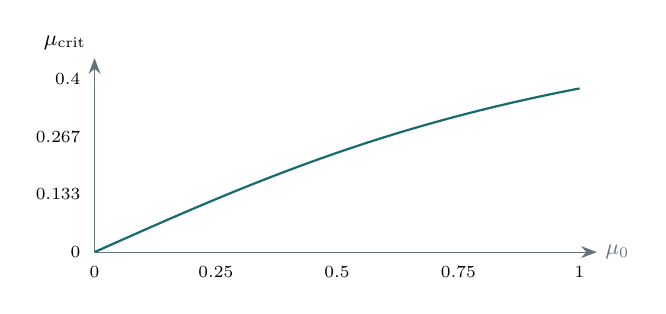
\begin{tikzpicture}[scale=.88,transform shape]
\draw[axis] (0,0.0000000)--(7.25,0.0000000) node[right] {$\mu_0$};
\draw[axis] (0.0000000,0)--(0.0000000,2.8);
\node[above left] at (0.0000000,2.8) {$\mu_{\rm crit}$};
\node[below,font=\scriptsize] at (0.0000000,-0.0800000) {$0$};
\node[below,font=\scriptsize] at (1.7500000,-0.0800000) {$0.25$};
\node[below,font=\scriptsize] at (3.5000000,-0.0800000) {$0.5$};
\node[below,font=\scriptsize] at (5.2500000,-0.0800000) {$0.75$};
\node[below,font=\scriptsize] at (7.0000000,-0.0800000) {$1$};
\node[left,font=\scriptsize] at (-0.0800000,0.0000000) {$0$};
\node[left,font=\scriptsize] at (-0.0800000,0.8333333) {$0.133$};
\node[left,font=\scriptsize] at (-0.0800000,1.6666667) {$0.267$};
\node[left,font=\scriptsize] at (-0.0800000,2.5000000) {$0.4$};
\draw[thick,color=accent] plot coordinates {(0.0000000,0.0000000) (0.0291667,0.0130207) (0.0583333,0.0260410) (0.0875000,0.0390602) (0.1166667,0.0520779) (0.1458333,0.0650936) (0.1750000,0.0781067) (0.2041667,0.0911168) (0.2333333,0.1041233) (0.2625000,0.1171258) (0.2916667,0.1301236) (0.3208333,0.1431165) (0.3500000,0.1561037) (0.3791667,0.1690849) (0.4083333,0.1820595) (0.4375000,0.1950270) (0.4666667,0.2079870) (0.4958333,0.2209389) (0.5250000,0.2338822) (0.5541667,0.2468164) (0.5833333,0.2597411) (0.6125000,0.2726558) (0.6416667,0.2855599) (0.6708333,0.2984531) (0.7000000,0.3113347) (0.7291667,0.3242043) (0.7583333,0.3370615) (0.7875000,0.3499057) (0.8166667,0.3627366) (0.8458333,0.3755535) (0.8750000,0.3883561) (0.9041667,0.4011439) (0.9333333,0.4139164) (0.9625000,0.4266731) (0.9916667,0.4394136) (1.0208333,0.4521375) (1.0500000,0.4648443) (1.0791667,0.4775335) (1.1083333,0.4902047) (1.1375000,0.5028574) (1.1666667,0.5154913) (1.1958333,0.5281059) (1.2250000,0.5407006) (1.2541667,0.5532752) (1.2833333,0.5658292) (1.3125000,0.5783622) (1.3416667,0.5908737) (1.3708333,0.6033634) (1.4000000,0.6158308) (1.4291667,0.6282755) (1.4583333,0.6406972) (1.4875000,0.6530953) (1.5166667,0.6654696) (1.5458333,0.6778197) (1.5750000,0.6901451) (1.6041667,0.7024455) (1.6333333,0.7147205) (1.6625000,0.7269697) (1.6916667,0.7391927) (1.7208333,0.7513893) (1.7500000,0.7635590) (1.7791667,0.7757015) (1.8083333,0.7878165) (1.8375000,0.7999035) (1.8666667,0.8119623) (1.8958333,0.8239924) (1.9250000,0.8359937) (1.9541667,0.8479657) (1.9833333,0.8599082) (2.0125000,0.8718208) (2.0416667,0.8837031) (2.0708333,0.8955550) (2.1000000,0.9073761) (2.1291667,0.9191661) (2.1583333,0.9309246) (2.1875000,0.9426515) (2.2166667,0.9543464) (2.2458333,0.9660091) (2.2750000,0.9776393) (2.3041667,0.9892366) (2.3333333,1.0008010) (2.3625000,1.0123320) (2.3916667,1.0238294) (2.4208333,1.0352930) (2.4500000,1.0467226) (2.4791667,1.0581179) (2.5083333,1.0694786) (2.5375000,1.0808046) (2.5666667,1.0920956) (2.5958333,1.1033514) (2.6250000,1.1145718) (2.6541667,1.1257566) (2.6833333,1.1369055) (2.7125000,1.1480184) (2.7416667,1.1590951) (2.7708333,1.1701353) (2.8000000,1.1811390) (2.8291667,1.1921059) (2.8583333,1.2030358) (2.8875000,1.2139286) (2.9166667,1.2247841) (2.9458333,1.2356021) (2.9750000,1.2463825) (3.0041667,1.2571252) (3.0333333,1.2678300) (3.0625000,1.2784967) (3.0916667,1.2891252) (3.1208333,1.2997154) (3.1500000,1.3102672) (3.1791667,1.3207803) (3.2083333,1.3312548) (3.2375000,1.3416905) (3.2666667,1.3520872) (3.2958333,1.3624450) (3.3250000,1.3727636) (3.3541667,1.3830429) (3.3833333,1.3932830) (3.4125000,1.4034836) (3.4416667,1.4136448) (3.4708333,1.4237664) (3.5000000,1.4338483) (3.5291667,1.4438906) (3.5583333,1.4538930) (3.5875000,1.4638556) (3.6166667,1.4737783) (3.6458333,1.4836610) (3.6750000,1.4935037) (3.7041667,1.5033063) (3.7333333,1.5130688) (3.7625000,1.5227912) (3.7916667,1.5324734) (3.8208333,1.5421154) (3.8500000,1.5517171) (3.8791667,1.5612786) (3.9083333,1.5707998) (3.9375000,1.5802806) (3.9666667,1.5897212) (3.9958333,1.5991214) (4.0250000,1.6084813) (4.0541667,1.6178008) (4.0833333,1.6270800) (4.1125000,1.6363189) (4.1416667,1.6455174) (4.1708333,1.6546756) (4.2000000,1.6637935) (4.2291667,1.6728710) (4.2583333,1.6819084) (4.2875000,1.6909054) (4.3166667,1.6998622) (4.3458333,1.7087789) (4.3750000,1.7176553) (4.4041667,1.7264917) (4.4333333,1.7352879) (4.4625000,1.7440441) (4.4916667,1.7527602) (4.5208333,1.7614364) (4.5500000,1.7700727) (4.5791667,1.7786691) (4.6083333,1.7872257) (4.6375000,1.7957425) (4.6666667,1.8042196) (4.6958333,1.8126571) (4.7250000,1.8210549) (4.7541667,1.8294133) (4.7833333,1.8377322) (4.8125000,1.8460118) (4.8416667,1.8542520) (4.8708333,1.8624531) (4.9000000,1.8706149) (4.9291667,1.8787377) (4.9583333,1.8868215) (4.9875000,1.8948664) (5.0166667,1.9028725) (5.0458333,1.9108398) (5.0750000,1.9187684) (5.1041667,1.9266586) (5.1333333,1.9345102) (5.1625000,1.9423235) (5.1916667,1.9500985) (5.2208333,1.9578353) (5.2500000,1.9655341) (5.2791667,1.9731948) (5.3083333,1.9808177) (5.3375000,1.9884029) (5.3666667,1.9959503) (5.3958333,2.0034602) (5.4250000,2.0109327) (5.4541667,2.0183678) (5.4833333,2.0257657) (5.5125000,2.0331265) (5.5416667,2.0404503) (5.5708333,2.0477372) (5.6000000,2.0549873) (5.6291667,2.0622008) (5.6583333,2.0693778) (5.6875000,2.0765184) (5.7166667,2.0836226) (5.7458333,2.0906907) (5.7750000,2.0977228) (5.8041667,2.1047189) (5.8333333,2.1116793) (5.8625000,2.1186040) (5.8916667,2.1254932) (5.9208333,2.1323469) (5.9500000,2.1391654) (5.9791667,2.1459487) (6.0083333,2.1526970) (6.0375000,2.1594105) (6.0666667,2.1660891) (6.0958333,2.1727332) (6.1250000,2.1793427) (6.1541667,2.1859179) (6.1833333,2.1924589) (6.2125000,2.1989658) (6.2416667,2.2054388) (6.2708333,2.2118780) (6.3000000,2.2182835) (6.3291667,2.2246554) (6.3583333,2.2309940) (6.3875000,2.2372993) (6.4166667,2.2435715) (6.4458333,2.2498107) (6.4750000,2.2560170) (6.5041667,2.2621907) (6.5333333,2.2683318) (6.5625000,2.2744405) (6.5916667,2.2805170) (6.6208333,2.2865613) (6.6500000,2.2925736) (6.6791667,2.2985540) (6.7083333,2.3045028) (6.7375000,2.3104200) (6.7666667,2.3163058) (6.7958333,2.3221602) (6.8250000,2.3279836) (6.8541667,2.3337760) (6.8833333,2.3395375) (6.9125000,2.3452683) (6.9416667,2.3509686) (6.9708333,2.3566384) (7.0000000,2.3622780)};
\end{tikzpicture}
\figcaption{变图综一.1V3\quad 内接触静摩擦的最低系数}
\end{minipage}\end{center}
变图综一.1V3显示临界值随地面摩擦增大，$\mu_0=1/2$时给$1/\sqrt{19}$，$\mu_0\to0$时按$\mu_0/2$趋零。地面提供的转动力矩越大，带动内盘同步所需的接触摩擦也越大。
\item \textbf{总耗散与接触面的分工。} 对$\mu=0.2$求两个阶段的总动能，并说明地面与内部接触各在何时产生热。
\par 将主解的$v,\omega_1,\omega_2$代入$K=2mv^2+mR^2\omega_1^2/4+15mR^2\omega_2^2/4$。在第一阶段，耗散功率为$f_2u_g+f_1u_i$；第二阶段$u_g=0$，只剩$f_1u_i$。初末状态分别给
\[
K_0=2mv_0^2,\qquad K_f=\frac43mv_0^2,\qquad Q_{\text{总}}=\frac23mv_0^2.
\]
\begin{center}\begin{minipage}{.98\linewidth}\centering
\begin{tikzpicture}[scale=.88,transform shape]
\draw[axis] (0,0.0000000)--(7.25,0.0000000) node[right] {$gt/v_0$};
\draw[axis] (0.0000000,0)--(0.0000000,2.8);
\node[above left] at (0.0000000,2.8) {$\text{能量}/(mv_0^2)$};
\node[below,font=\scriptsize] at (0.0000000,-0.0800000) {$0$};
\node[below,font=\scriptsize] at (1.7500000,-0.0800000) {$0.225$};
\node[below,font=\scriptsize] at (3.5000000,-0.0800000) {$0.45$};
\node[below,font=\scriptsize] at (5.2500000,-0.0800000) {$0.675$};
\node[below,font=\scriptsize] at (7.0000000,-0.0800000) {$0.9$};
\node[left,font=\scriptsize] at (-0.0800000,0.0000000) {$0$};
\node[left,font=\scriptsize] at (-0.0800000,0.8333333) {$0.7$};
\node[left,font=\scriptsize] at (-0.0800000,1.6666667) {$1.4$};
\node[left,font=\scriptsize] at (-0.0800000,2.5000000) {$2.1$};
\draw[thick,color=accent] plot coordinates {(0.0000000,2.3809524) (0.0291667,2.3720489) (0.0583333,2.3631958) (0.0875000,2.3543928) (0.1166667,2.3456402) (0.1458333,2.3369377) (0.1750000,2.3282856) (0.2041667,2.3196837) (0.2333333,2.3111320) (0.2625000,2.3026306) (0.2916667,2.2941795) (0.3208333,2.2857786) (0.3500000,2.2774280) (0.3791667,2.2691277) (0.4083333,2.2608776) (0.4375000,2.2526777) (0.4666667,2.2445281) (0.4958333,2.2364288) (0.5250000,2.2283797) (0.5541667,2.2203809) (0.5833333,2.2124323) (0.6125000,2.2045340) (0.6416667,2.1966860) (0.6708333,2.1888882) (0.7000000,2.1811407) (0.7291667,2.1734434) (0.7583333,2.1657964) (0.7875000,2.1581996) (0.8166667,2.1506531) (0.8458333,2.1431569) (0.8750000,2.1357109) (0.9041667,2.1283151) (0.9333333,2.1209697) (0.9625000,2.1136744) (0.9916667,2.1064295) (1.0208333,2.0992348) (1.0500000,2.0920903) (1.0791667,2.0849961) (1.1083333,2.0779522) (1.1375000,2.0709585) (1.1666667,2.0640151) (1.1958333,2.0571219) (1.2250000,2.0502790) (1.2541667,2.0434864) (1.2833333,2.0367440) (1.3125000,2.0300518) (1.3416667,2.0234100) (1.3708333,2.0168183) (1.4000000,2.0102770) (1.4291667,2.0037859) (1.4583333,1.9973450) (1.4875000,1.9909544) (1.5166667,1.9846141) (1.5458333,1.9783240) (1.5750000,1.9720842) (1.6041667,1.9658946) (1.6333333,1.9597553) (1.6625000,1.9536662) (1.6916667,1.9476274) (1.7208333,1.9416389) (1.7500000,1.9357006) (1.7791667,1.9298126) (1.8083333,1.9239748) (1.8375000,1.9181873) (1.8666667,1.9124500) (1.8958333,1.9067631) (1.9250000,1.9011263) (1.9541667,1.8955398) (1.9833333,1.8900036) (2.0125000,1.8845176) (2.0416667,1.8790819) (2.0708333,1.8736965) (2.1000000,1.8683613) (2.1291667,1.8630763) (2.1583333,1.8578416) (2.1875000,1.8526572) (2.2166667,1.8475230) (2.2458333,1.8424391) (2.2750000,1.8374055) (2.3041667,1.8324221) (2.3333333,1.8274889) (2.3625000,1.8226060) (2.3916667,1.8177734) (2.4208333,1.8129910) (2.4500000,1.8082589) (2.4791667,1.8035771) (2.5083333,1.7989454) (2.5375000,1.7943641) (2.5666667,1.7898330) (2.5958333,1.7853522) (2.6250000,1.7809216) (2.6541667,1.7765413) (2.6833333,1.7722112) (2.7125000,1.7679314) (2.7416667,1.7637019) (2.7708333,1.7595226) (2.8000000,1.7553936) (2.8291667,1.7513148) (2.8583333,1.7472863) (2.8875000,1.7433080) (2.9166667,1.7393800) (2.9458333,1.7355023) (2.9750000,1.7316748) (3.0041667,1.7278975) (3.0333333,1.7241706) (3.0625000,1.7204938) (3.0916667,1.7168674) (3.1208333,1.7132912) (3.1500000,1.7097652) (3.1791667,1.7062895) (3.2083333,1.7028641) (3.2375000,1.6994889) (3.2666667,1.6961640) (3.2958333,1.6928893) (3.3250000,1.6896649) (3.3541667,1.6864908) (3.3833333,1.6833669) (3.4125000,1.6802932) (3.4416667,1.6772699) (3.4708333,1.6742967) (3.5000000,1.6713739) (3.5291667,1.6685013) (3.5583333,1.6656789) (3.5875000,1.6629068) (3.6166667,1.6601850) (3.6458333,1.6575134) (3.6750000,1.6548921) (3.7041667,1.6523210) (3.7333333,1.6498002) (3.7625000,1.6473296) (3.7916667,1.6449093) (3.8208333,1.6425393) (3.8500000,1.6402195) (3.8791667,1.6379500) (3.9083333,1.6357307) (3.9375000,1.6335617) (3.9666667,1.6314430) (3.9958333,1.6293745) (4.0250000,1.6273562) (4.0541667,1.6253882) (4.0833333,1.6234705) (4.1125000,1.6216030) (4.1416667,1.6197858) (4.1708333,1.6180189) (4.2000000,1.6163022) (4.2291667,1.6146357) (4.2583333,1.6130196) (4.2875000,1.6114536) (4.3166667,1.6099380) (4.3458333,1.6084725) (4.3750000,1.6070574) (4.4041667,1.6056925) (4.4333333,1.6043778) (4.4625000,1.6031135) (4.4916667,1.6018993) (4.5208333,1.6007355) (4.5500000,1.5996218) (4.5791667,1.5985585) (4.6083333,1.5975454) (4.6375000,1.5965825) (4.6666667,1.5956699) (4.6958333,1.5948076) (4.7250000,1.5939955) (4.7541667,1.5932337) (4.7833333,1.5925222) (4.8125000,1.5918609) (4.8416667,1.5912498) (4.8708333,1.5906890) (4.9000000,1.5901785) (4.9291667,1.5897182) (4.9583333,1.5893082) (4.9875000,1.5889484) (5.0166667,1.5886389) (5.0458333,1.5883797) (5.0750000,1.5881707) (5.1041667,1.5880120) (5.1333333,1.5879035) (5.1625000,1.5878452) (5.1916667,1.5878081) (5.2208333,1.5877722) (5.2500000,1.5877377) (5.2791667,1.5877045) (5.3083333,1.5876726) (5.3375000,1.5876420) (5.3666667,1.5876127) (5.3958333,1.5875848) (5.4250000,1.5875581) (5.4541667,1.5875328) (5.4833333,1.5875088) (5.5125000,1.5874861) (5.5416667,1.5874647) (5.5708333,1.5874447) (5.6000000,1.5874259) (5.6291667,1.5874085) (5.6583333,1.5873924) (5.6875000,1.5873776) (5.7166667,1.5873641) (5.7458333,1.5873519) (5.7750000,1.5873411) (5.8041667,1.5873316) (5.8333333,1.5873233) (5.8625000,1.5873164) (5.8916667,1.5873108) (5.9208333,1.5873066) (5.9500000,1.5873036) (5.9791667,1.5873020) (6.0083333,1.5873016) (6.0375000,1.5873016) (6.0666667,1.5873016) (6.0958333,1.5873016) (6.1250000,1.5873016) (6.1541667,1.5873016) (6.1833333,1.5873016) (6.2125000,1.5873016) (6.2416667,1.5873016) (6.2708333,1.5873016) (6.3000000,1.5873016) (6.3291667,1.5873016) (6.3583333,1.5873016) (6.3875000,1.5873016) (6.4166667,1.5873016) (6.4458333,1.5873016) (6.4750000,1.5873016) (6.5041667,1.5873016) (6.5333333,1.5873016) (6.5625000,1.5873016) (6.5916667,1.5873016) (6.6208333,1.5873016) (6.6500000,1.5873016) (6.6791667,1.5873016) (6.7083333,1.5873016) (6.7375000,1.5873016) (6.7666667,1.5873016) (6.7958333,1.5873016) (6.8250000,1.5873016) (6.8541667,1.5873016) (6.8833333,1.5873016) (6.9125000,1.5873016) (6.9416667,1.5873016) (6.9708333,1.5873016) (7.0000000,1.5873016)};
\draw[thick,color=accent] (7.65,2.4)--(8.1,2.4);\node[right,font=\scriptsize] at (8.15,2.4) {$K$};
\draw[thick,dashed,color=warm] plot coordinates {(0.0000000,0.0000000) (0.0291667,0.0089034) (0.0583333,0.0177566) (0.0875000,0.0265596) (0.1166667,0.0353122) (0.1458333,0.0440146) (0.1750000,0.0526668) (0.2041667,0.0612687) (0.2333333,0.0698203) (0.2625000,0.0783217) (0.2916667,0.0867729) (0.3208333,0.0951737) (0.3500000,0.1035244) (0.3791667,0.1118247) (0.4083333,0.1200748) (0.4375000,0.1282747) (0.4666667,0.1364243) (0.4958333,0.1445236) (0.5250000,0.1525727) (0.5541667,0.1605715) (0.5833333,0.1685200) (0.6125000,0.1764183) (0.6416667,0.1842664) (0.6708333,0.1920642) (0.7000000,0.1998117) (0.7291667,0.2075090) (0.7583333,0.2151560) (0.7875000,0.2227528) (0.8166667,0.2302993) (0.8458333,0.2377955) (0.8750000,0.2452415) (0.9041667,0.2526372) (0.9333333,0.2599827) (0.9625000,0.2672779) (0.9916667,0.2745229) (1.0208333,0.2817176) (1.0500000,0.2888621) (1.0791667,0.2959563) (1.1083333,0.3030002) (1.1375000,0.3099939) (1.1666667,0.3169373) (1.1958333,0.3238305) (1.2250000,0.3306734) (1.2541667,0.3374660) (1.2833333,0.3442084) (1.3125000,0.3509005) (1.3416667,0.3575424) (1.3708333,0.3641341) (1.4000000,0.3706754) (1.4291667,0.3771665) (1.4583333,0.3836074) (1.4875000,0.3899980) (1.5166667,0.3963383) (1.5458333,0.4026284) (1.5750000,0.4088682) (1.6041667,0.4150578) (1.6333333,0.4211971) (1.6625000,0.4272862) (1.6916667,0.4333249) (1.7208333,0.4393135) (1.7500000,0.4452518) (1.7791667,0.4511398) (1.8083333,0.4569776) (1.8375000,0.4627651) (1.8666667,0.4685023) (1.8958333,0.4741893) (1.9250000,0.4798261) (1.9541667,0.4854126) (1.9833333,0.4909488) (2.0125000,0.4964348) (2.0416667,0.5018705) (2.0708333,0.5072559) (2.1000000,0.5125911) (2.1291667,0.5178761) (2.1583333,0.5231107) (2.1875000,0.5282952) (2.2166667,0.5334293) (2.2458333,0.5385133) (2.2750000,0.5435469) (2.3041667,0.5485303) (2.3333333,0.5534635) (2.3625000,0.5583464) (2.3916667,0.5631790) (2.4208333,0.5679614) (2.4500000,0.5726935) (2.4791667,0.5773753) (2.5083333,0.5820069) (2.5375000,0.5865883) (2.5666667,0.5911194) (2.5958333,0.5956002) (2.6250000,0.6000308) (2.6541667,0.6044111) (2.6833333,0.6087411) (2.7125000,0.6130210) (2.7416667,0.6172505) (2.7708333,0.6214298) (2.8000000,0.6255588) (2.8291667,0.6296376) (2.8583333,0.6336661) (2.8875000,0.6376444) (2.9166667,0.6415724) (2.9458333,0.6454501) (2.9750000,0.6492776) (3.0041667,0.6530549) (3.0333333,0.6567818) (3.0625000,0.6604585) (3.0916667,0.6640850) (3.1208333,0.6676612) (3.1500000,0.6711872) (3.1791667,0.6746629) (3.2083333,0.6780883) (3.2375000,0.6814635) (3.2666667,0.6847884) (3.2958333,0.6880631) (3.3250000,0.6912875) (3.3541667,0.6944616) (3.3833333,0.6975855) (3.4125000,0.7006591) (3.4416667,0.7036825) (3.4708333,0.7066556) (3.5000000,0.7095785) (3.5291667,0.7124511) (3.5583333,0.7152735) (3.5875000,0.7180456) (3.6166667,0.7207674) (3.6458333,0.7234390) (3.6750000,0.7260603) (3.7041667,0.7286314) (3.7333333,0.7311522) (3.7625000,0.7336227) (3.7916667,0.7360430) (3.8208333,0.7384131) (3.8500000,0.7407329) (3.8791667,0.7430024) (3.9083333,0.7452217) (3.9375000,0.7473907) (3.9666667,0.7495094) (3.9958333,0.7515779) (4.0250000,0.7535962) (4.0541667,0.7555641) (4.0833333,0.7574819) (4.1125000,0.7593493) (4.1416667,0.7611665) (4.1708333,0.7629335) (4.2000000,0.7646502) (4.2291667,0.7663166) (4.2583333,0.7679328) (4.2875000,0.7694988) (4.3166667,0.7710144) (4.3458333,0.7724798) (4.3750000,0.7738950) (4.4041667,0.7752599) (4.4333333,0.7765745) (4.4625000,0.7778389) (4.4916667,0.7790531) (4.5208333,0.7802169) (4.5500000,0.7813305) (4.5791667,0.7823939) (4.6083333,0.7834070) (4.6375000,0.7843698) (4.6666667,0.7852824) (4.6958333,0.7861448) (4.7250000,0.7869568) (4.7541667,0.7877187) (4.7833333,0.7884302) (4.8125000,0.7890915) (4.8416667,0.7897026) (4.8708333,0.7902634) (4.9000000,0.7907739) (4.9291667,0.7912342) (4.9583333,0.7916442) (4.9875000,0.7920039) (5.0166667,0.7923134) (5.0458333,0.7925727) (5.0750000,0.7927817) (5.1041667,0.7929404) (5.1333333,0.7930489) (5.1625000,0.7931071) (5.1916667,0.7931443) (5.2208333,0.7931801) (5.2500000,0.7932147) (5.2791667,0.7932479) (5.3083333,0.7932798) (5.3375000,0.7933104) (5.3666667,0.7933396) (5.3958333,0.7933676) (5.4250000,0.7933942) (5.4541667,0.7934196) (5.4833333,0.7934436) (5.5125000,0.7934663) (5.5416667,0.7934876) (5.5708333,0.7935077) (5.6000000,0.7935264) (5.6291667,0.7935439) (5.6583333,0.7935600) (5.6875000,0.7935748) (5.7166667,0.7935883) (5.7458333,0.7936004) (5.7750000,0.7936113) (5.8041667,0.7936208) (5.8333333,0.7936291) (5.8625000,0.7936360) (5.8916667,0.7936415) (5.9208333,0.7936458) (5.9500000,0.7936488) (5.9791667,0.7936504) (6.0083333,0.7936508) (6.0375000,0.7936508) (6.0666667,0.7936508) (6.0958333,0.7936508) (6.1250000,0.7936508) (6.1541667,0.7936508) (6.1833333,0.7936508) (6.2125000,0.7936508) (6.2416667,0.7936508) (6.2708333,0.7936508) (6.3000000,0.7936508) (6.3291667,0.7936508) (6.3583333,0.7936508) (6.3875000,0.7936508) (6.4166667,0.7936508) (6.4458333,0.7936508) (6.4750000,0.7936508) (6.5041667,0.7936508) (6.5333333,0.7936508) (6.5625000,0.7936508) (6.5916667,0.7936508) (6.6208333,0.7936508) (6.6500000,0.7936508) (6.6791667,0.7936508) (6.7083333,0.7936508) (6.7375000,0.7936508) (6.7666667,0.7936508) (6.7958333,0.7936508) (6.8250000,0.7936508) (6.8541667,0.7936508) (6.8833333,0.7936508) (6.9125000,0.7936508) (6.9416667,0.7936508) (6.9708333,0.7936508) (7.0000000,0.7936508)};
\draw[thick,dashed,color=warm] (7.65,1.9)--(8.1,1.9);\node[right,font=\scriptsize] at (8.15,1.9) {$Q$};
\end{tikzpicture}
\figcaption{变图综一.1V4\quad 地面滚动以后内部滑动仍继续耗散}
\end{minipage}\end{center}
变图综一.1V4画$K/(mv_0^2)$和$Q/(mv_0^2)$，二者之和恒为2。第二阶段的能量下降较小但持续到两转速相等；地面静摩擦通过约束参与动量和角动量的重新分配，接触点速度为零使该处的瞬时功率为零。
\item \textbf{内摩擦趋于零时的持续时间。} 在$0<\mu<1/\sqrt{19}$内求第二阶段时长，并讨论$\mu\to0^+$。
\par 令$\xi=\sqrt5\mu/\sqrt{1+\mu^2}$，$s_1=gt_1/v_0=30/(47-4\xi)$，$A_2=a_2/g=4\mu/\sqrt{2209+2193\mu^2}$。第一阶段末转速差为$R(\omega_{21}-\omega_{11})/v_0=(8-16\xi)s_1/15$，所以
\[
\frac{g\Delta t}{v_0}=\frac{(8-16\xi)s_1}{360A_2}.
\]
\begin{center}\begin{minipage}{.98\linewidth}\centering
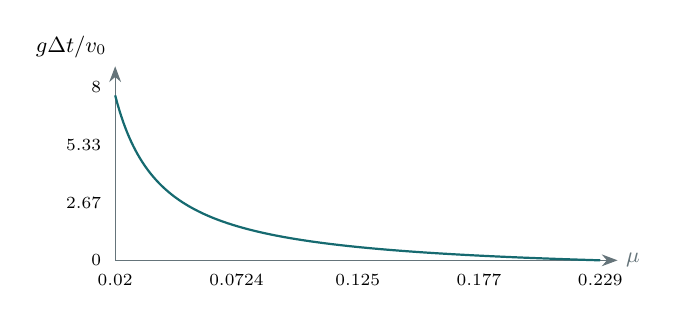
\begin{tikzpicture}[scale=.88,transform shape]
\draw[axis] (0,0.0000000)--(7.25,0.0000000) node[right] {$\mu$};
\draw[axis] (0.0000000,0)--(0.0000000,2.8);
\node[above left] at (0.0000000,2.8) {$g\Delta t/v_0$};
\node[below,font=\scriptsize] at (0.0000000,-0.0800000) {$0.02$};
\node[below,font=\scriptsize] at (1.7500000,-0.0800000) {$0.0724$};
\node[below,font=\scriptsize] at (3.5000000,-0.0800000) {$0.125$};
\node[below,font=\scriptsize] at (5.2500000,-0.0800000) {$0.177$};
\node[below,font=\scriptsize] at (7.0000000,-0.0800000) {$0.229$};
\node[left,font=\scriptsize] at (-0.0800000,0.0000000) {$0$};
\node[left,font=\scriptsize] at (-0.0800000,0.8333333) {$2.67$};
\node[left,font=\scriptsize] at (-0.0800000,1.6666667) {$5.33$};
\node[left,font=\scriptsize] at (-0.0800000,2.5000000) {$8$};
\draw[thick,color=accent] plot coordinates {(0.0000000,2.3808200) (0.0291667,2.2719396) (0.0583333,2.1717961) (0.0875000,2.0793783) (0.1166667,1.9938253) (0.1458333,1.9143994) (0.1750000,1.8404651) (0.2041667,1.7714718) (0.2333333,1.7069401) (0.2625000,1.6464507) (0.2916667,1.5896352) (0.3208333,1.5361688) (0.3500000,1.4857636) (0.3791667,1.4381640) (0.4083333,1.3931421) (0.4375000,1.3504939) (0.4666667,1.3100364) (0.4958333,1.2716051) (0.5250000,1.2350514) (0.5541667,1.2002409) (0.5833333,1.1670517) (0.6125000,1.1353732) (0.6416667,1.1051045) (0.6708333,1.0761533) (0.7000000,1.0484356) (0.7291667,1.0218741) (0.7583333,0.9963978) (0.7875000,0.9719416) (0.8166667,0.9484453) (0.8458333,0.9258536) (0.8750000,0.9041150) (0.9041667,0.8831822) (0.9333333,0.8630112) (0.9625000,0.8435610) (0.9916667,0.8247937) (1.0208333,0.8066739) (1.0500000,0.7891686) (1.0791667,0.7722471) (1.1083333,0.7558806) (1.1375000,0.7400423) (1.1666667,0.7247069) (1.1958333,0.7098508) (1.2250000,0.6954520) (1.2541667,0.6814895) (1.2833333,0.6679439) (1.3125000,0.6547966) (1.3416667,0.6420305) (1.3708333,0.6296291) (1.4000000,0.6175769) (1.4291667,0.6058595) (1.4583333,0.5944630) (1.4875000,0.5833745) (1.5166667,0.5725815) (1.5458333,0.5620725) (1.5750000,0.5518363) (1.6041667,0.5418625) (1.6333333,0.5321410) (1.6625000,0.5226624) (1.6916667,0.5134177) (1.7208333,0.5043983) (1.7500000,0.4955960) (1.7791667,0.4870032) (1.8083333,0.4786124) (1.8375000,0.4704166) (1.8666667,0.4624089) (1.8958333,0.4545831) (1.9250000,0.4469330) (1.9541667,0.4394526) (1.9833333,0.4321365) (2.0125000,0.4249792) (2.0416667,0.4179756) (2.0708333,0.4111208) (2.1000000,0.4044102) (2.1291667,0.3978391) (2.1583333,0.3914033) (2.1875000,0.3850986) (2.2166667,0.3789211) (2.2458333,0.3728669) (2.2750000,0.3669324) (2.3041667,0.3611141) (2.3333333,0.3554085) (2.3625000,0.3498124) (2.3916667,0.3443227) (2.4208333,0.3389363) (2.4500000,0.3336505) (2.4791667,0.3284622) (2.5083333,0.3233690) (2.5375000,0.3183682) (2.5666667,0.3134572) (2.5958333,0.3086337) (2.6250000,0.3038954) (2.6541667,0.2992400) (2.6833333,0.2946653) (2.7125000,0.2901693) (2.7416667,0.2857499) (2.7708333,0.2814052) (2.8000000,0.2771333) (2.8291667,0.2729324) (2.8583333,0.2688008) (2.8875000,0.2647366) (2.9166667,0.2607383) (2.9458333,0.2568043) (2.9750000,0.2529331) (3.0041667,0.2491230) (3.0333333,0.2453728) (3.0625000,0.2416810) (3.0916667,0.2380461) (3.1208333,0.2344670) (3.1500000,0.2309424) (3.1791667,0.2274709) (3.2083333,0.2240514) (3.2375000,0.2206828) (3.2666667,0.2173638) (3.2958333,0.2140935) (3.3250000,0.2108707) (3.3541667,0.2076944) (3.3833333,0.2045636) (3.4125000,0.2014774) (3.4416667,0.1984347) (3.4708333,0.1954347) (3.5000000,0.1924764) (3.5291667,0.1895591) (3.5583333,0.1866817) (3.5875000,0.1838436) (3.6166667,0.1810440) (3.6458333,0.1782819) (3.6750000,0.1755568) (3.7041667,0.1728678) (3.7333333,0.1702142) (3.7625000,0.1675953) (3.7916667,0.1650105) (3.8208333,0.1624591) (3.8500000,0.1599404) (3.8791667,0.1574539) (3.9083333,0.1549988) (3.9375000,0.1525746) (3.9666667,0.1501807) (3.9958333,0.1478165) (4.0250000,0.1454816) (4.0541667,0.1431753) (4.0833333,0.1408971) (4.1125000,0.1386465) (4.1416667,0.1364231) (4.1708333,0.1342262) (4.2000000,0.1320555) (4.2291667,0.1299104) (4.2583333,0.1277906) (4.2875000,0.1256955) (4.3166667,0.1236247) (4.3458333,0.1215779) (4.3750000,0.1195545) (4.4041667,0.1175543) (4.4333333,0.1155767) (4.4625000,0.1136214) (4.4916667,0.1116881) (4.5208333,0.1097763) (4.5500000,0.1078857) (4.5791667,0.1060160) (4.6083333,0.1041668) (4.6375000,0.1023377) (4.6666667,0.1005284) (4.6958333,0.0987387) (4.7250000,0.0969681) (4.7541667,0.0952164) (4.7833333,0.0934833) (4.8125000,0.0917685) (4.8416667,0.0900716) (4.8708333,0.0883925) (4.9000000,0.0867308) (4.9291667,0.0850863) (4.9583333,0.0834586) (4.9875000,0.0818476) (5.0166667,0.0802529) (5.0458333,0.0786743) (5.0750000,0.0771117) (5.1041667,0.0755646) (5.1333333,0.0740330) (5.1625000,0.0725165) (5.1916667,0.0710150) (5.2208333,0.0695282) (5.2500000,0.0680559) (5.2791667,0.0665979) (5.3083333,0.0651539) (5.3375000,0.0637239) (5.3666667,0.0623075) (5.3958333,0.0609045) (5.4250000,0.0595149) (5.4541667,0.0581384) (5.4833333,0.0567747) (5.5125000,0.0554238) (5.5416667,0.0540855) (5.5708333,0.0527595) (5.6000000,0.0514457) (5.6291667,0.0501439) (5.6583333,0.0488540) (5.6875000,0.0475758) (5.7166667,0.0463091) (5.7458333,0.0450538) (5.7750000,0.0438097) (5.8041667,0.0425767) (5.8333333,0.0413546) (5.8625000,0.0401433) (5.8916667,0.0389427) (5.9208333,0.0377525) (5.9500000,0.0365727) (5.9791667,0.0354031) (6.0083333,0.0342436) (6.0375000,0.0330941) (6.0666667,0.0319543) (6.0958333,0.0308243) (6.1250000,0.0297038) (6.1541667,0.0285928) (6.1833333,0.0274911) (6.2125000,0.0263987) (6.2416667,0.0253153) (6.2708333,0.0242409) (6.3000000,0.0231754) (6.3291667,0.0221186) (6.3583333,0.0210705) (6.3875000,0.0200309) (6.4166667,0.0189998) (6.4458333,0.0179769) (6.4750000,0.0169623) (6.5041667,0.0159559) (6.5333333,0.0149575) (6.5625000,0.0139670) (6.5916667,0.0129843) (6.6208333,0.0120094) (6.6500000,0.0110421) (6.6791667,0.0100824) (6.7083333,0.0091302) (6.7375000,0.0081853) (6.7666667,0.0072478) (6.7958333,0.0063174) (6.8250000,0.0053942) (6.8541667,0.0044780) (6.8833333,0.0035688) (6.9125000,0.0026665) (6.9416667,0.0017710) (6.9708333,0.0008822) (7.0000000,0.0000000)};
\end{tikzpicture}
\figcaption{变图综一.1V5\quad 微小内摩擦需要更长时间使两转速相等}
\end{minipage}\end{center}
变图综一.1V5显示第二阶段时长在临界点趋零，在$\mu\to0^+$时发散。此时$s_1\to30/47$，$A_2\sim4\mu/47$，故$g\Delta t/v_0\sim1/(6\mu)$。每个正$\mu$都可在足够长时间后达到共同转速；$\mu=0$时的转速差则永久保留。
\item \textbf{接触点的方向。} 对$\mu=0.2$，以$a/g=A$为横坐标，求内接触点$P$的水平坐标，说明两个阶段的接触位置。
\par 法向单位矢量满足$N_1(\boldsymbol n+\mu\boldsymbol t)=mg(-A,1)$，$\boldsymbol t=(-n_y,n_x)$。解得
\[
\frac{x_P}{R}=\frac{A-\mu}{\sqrt{(1+A^2)(1+\mu^2)}},\qquad
\frac{y_P}{R}=-\frac{1+\mu A}{\sqrt{(1+A^2)(1+\mu^2)}}.
\]
\begin{center}\begin{minipage}{.98\linewidth}\centering
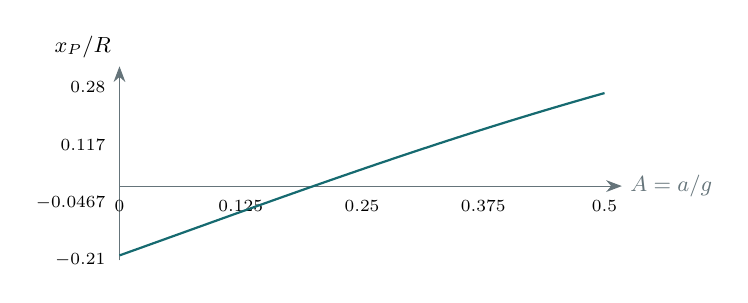
\begin{tikzpicture}[scale=.88,transform shape]
\draw[axis] (0,1.0714286)--(7.25,1.0714286) node[right] {$A=a/g$};
\draw[axis] (0.0000000,0)--(0.0000000,2.8);
\node[above left] at (0.0000000,2.8) {$x_P/R$};
\node[below,font=\scriptsize] at (0.0000000,0.9914286) {$0$};
\node[below,font=\scriptsize] at (1.7500000,0.9914286) {$0.125$};
\node[below,font=\scriptsize] at (3.5000000,0.9914286) {$0.25$};
\node[below,font=\scriptsize] at (5.2500000,0.9914286) {$0.375$};
\node[below,font=\scriptsize] at (7.0000000,0.9914286) {$0.5$};
\node[left,font=\scriptsize] at (-0.0800000,0.0000000) {$-0.21$};
\node[left,font=\scriptsize] at (-0.0800000,0.8333333) {$-0.0467$};
\node[left,font=\scriptsize] at (-0.0800000,1.6666667) {$0.117$};
\node[left,font=\scriptsize] at (-0.0800000,2.5000000) {$0.28$};
\draw[thick,color=accent] plot coordinates {(0.0000000,0.0708360) (0.0291667,0.0812610) (0.0583333,0.0916902) (0.0875000,0.1021235) (0.1166667,0.1125607) (0.1458333,0.1230017) (0.1750000,0.1334464) (0.2041667,0.1438945) (0.2333333,0.1543461) (0.2625000,0.1648009) (0.2916667,0.1752589) (0.3208333,0.1857198) (0.3500000,0.1961836) (0.3791667,0.2066501) (0.4083333,0.2171191) (0.4375000,0.2275906) (0.4666667,0.2380643) (0.4958333,0.2485402) (0.5250000,0.2590182) (0.5541667,0.2694980) (0.5833333,0.2799795) (0.6125000,0.2904627) (0.6416667,0.3009473) (0.6708333,0.3114333) (0.7000000,0.3219205) (0.7291667,0.3324087) (0.7583333,0.3428978) (0.7875000,0.3533878) (0.8166667,0.3638783) (0.8458333,0.3743694) (0.8750000,0.3848609) (0.9041667,0.3953525) (0.9333333,0.4058443) (0.9625000,0.4163361) (0.9916667,0.4268276) (1.0208333,0.4373189) (1.0500000,0.4478097) (1.0791667,0.4582999) (1.1083333,0.4687894) (1.1375000,0.4792781) (1.1666667,0.4897658) (1.1958333,0.5002523) (1.2250000,0.5107376) (1.2541667,0.5212215) (1.2833333,0.5317038) (1.3125000,0.5421845) (1.3416667,0.5526634) (1.3708333,0.5631403) (1.4000000,0.5736152) (1.4291667,0.5840879) (1.4583333,0.5945582) (1.4875000,0.6050261) (1.5166667,0.6154913) (1.5458333,0.6259539) (1.5750000,0.6364135) (1.6041667,0.6468702) (1.6333333,0.6573237) (1.6625000,0.6677740) (1.6916667,0.6782208) (1.7208333,0.6886642) (1.7500000,0.6991039) (1.7791667,0.7095398) (1.8083333,0.7199718) (1.8375000,0.7303997) (1.8666667,0.7408235) (1.8958333,0.7512430) (1.9250000,0.7616580) (1.9541667,0.7720685) (1.9833333,0.7824743) (2.0125000,0.7928752) (2.0416667,0.8032713) (2.0708333,0.8136622) (2.1000000,0.8240480) (2.1291667,0.8344284) (2.1583333,0.8448034) (2.1875000,0.8551729) (2.2166667,0.8655366) (2.2458333,0.8758945) (2.2750000,0.8862465) (2.3041667,0.8965924) (2.3333333,0.9069322) (2.3625000,0.9172656) (2.3916667,0.9275926) (2.4208333,0.9379130) (2.4500000,0.9482268) (2.4791667,0.9585338) (2.5083333,0.9688339) (2.5375000,0.9791269) (2.5666667,0.9894128) (2.5958333,0.9996914) (2.6250000,1.0099627) (2.6541667,1.0202264) (2.6833333,1.0304825) (2.7125000,1.0407309) (2.7416667,1.0509715) (2.7708333,1.0612041) (2.8000000,1.0714286) (2.8291667,1.0816449) (2.8583333,1.0918529) (2.8875000,1.1020525) (2.9166667,1.1122436) (2.9458333,1.1224260) (2.9750000,1.1325997) (3.0041667,1.1427646) (3.0333333,1.1529204) (3.0625000,1.1630672) (3.0916667,1.1732048) (3.1208333,1.1833331) (3.1500000,1.1934521) (3.1791667,1.2035615) (3.2083333,1.2136613) (3.2375000,1.2237513) (3.2666667,1.2338316) (3.2958333,1.2439020) (3.3250000,1.2539623) (3.3541667,1.2640125) (3.3833333,1.2740524) (3.4125000,1.2840820) (3.4416667,1.2941012) (3.4708333,1.3041099) (3.5000000,1.3141079) (3.5291667,1.3240952) (3.5583333,1.3340717) (3.5875000,1.3440372) (3.6166667,1.3539917) (3.6458333,1.3639351) (3.6750000,1.3738673) (3.7041667,1.3837882) (3.7333333,1.3936977) (3.7625000,1.4035957) (3.7916667,1.4134821) (3.8208333,1.4233569) (3.8500000,1.4332198) (3.8791667,1.4430709) (3.9083333,1.4529101) (3.9375000,1.4627372) (3.9666667,1.4725522) (3.9958333,1.4823550) (4.0250000,1.4921455) (4.0541667,1.5019236) (4.0833333,1.5116893) (4.1125000,1.5214424) (4.1416667,1.5311828) (4.1708333,1.5409106) (4.2000000,1.5506255) (4.2291667,1.5603275) (4.2583333,1.5700166) (4.2875000,1.5796926) (4.3166667,1.5893556) (4.3458333,1.5990053) (4.3750000,1.6086417) (4.4041667,1.6182648) (4.4333333,1.6278744) (4.4625000,1.6374705) (4.4916667,1.6470530) (4.5208333,1.6566219) (4.5500000,1.6661771) (4.5791667,1.6757184) (4.6083333,1.6852459) (4.6375000,1.6947594) (4.6666667,1.7042588) (4.6958333,1.7137442) (4.7250000,1.7232155) (4.7541667,1.7326725) (4.7833333,1.7421152) (4.8125000,1.7515436) (4.8416667,1.7609575) (4.8708333,1.7703569) (4.9000000,1.7797418) (4.9291667,1.7891120) (4.9583333,1.7984676) (4.9875000,1.8078084) (5.0166667,1.8171344) (5.0458333,1.8264455) (5.0750000,1.8357417) (5.1041667,1.8450229) (5.1333333,1.8542891) (5.1625000,1.8635401) (5.1916667,1.8727760) (5.2208333,1.8819967) (5.2500000,1.8912021) (5.2791667,1.9003921) (5.3083333,1.9095667) (5.3375000,1.9187260) (5.3666667,1.9278697) (5.3958333,1.9369978) (5.4250000,1.9461104) (5.4541667,1.9552073) (5.4833333,1.9642885) (5.5125000,1.9733540) (5.5416667,1.9824037) (5.5708333,1.9914375) (5.6000000,2.0004554) (5.6291667,2.0094574) (5.6583333,2.0184434) (5.6875000,2.0274133) (5.7166667,2.0363672) (5.7458333,2.0453050) (5.7750000,2.0542266) (5.8041667,2.0631320) (5.8333333,2.0720211) (5.8625000,2.0808939) (5.8916667,2.0897505) (5.9208333,2.0985906) (5.9500000,2.1074143) (5.9791667,2.1162216) (6.0083333,2.1250124) (6.0375000,2.1337867) (6.0666667,2.1425444) (6.0958333,2.1512855) (6.1250000,2.1600100) (6.1541667,2.1687179) (6.1833333,2.1774090) (6.2125000,2.1860834) (6.2416667,2.1947410) (6.2708333,2.2033819) (6.3000000,2.2120059) (6.3291667,2.2206130) (6.3583333,2.2292033) (6.3875000,2.2377766) (6.4166667,2.2463331) (6.4458333,2.2548725) (6.4750000,2.2633949) (6.5041667,2.2719003) (6.5333333,2.2803887) (6.5625000,2.2888599) (6.5916667,2.2973141) (6.6208333,2.3057512) (6.6500000,2.3141711) (6.6791667,2.3225738) (6.7083333,2.3309593) (6.7375000,2.3393276) (6.7666667,2.3476787) (6.7958333,2.3560125) (6.8250000,2.3643290) (6.8541667,2.3726283) (6.8833333,2.3809102) (6.9125000,2.3891748) (6.9416667,2.3974220) (6.9708333,2.4056518) (7.0000000,2.4138643)};
\end{tikzpicture}
\figcaption{变图综一.1V6\quad 加速度改变时内接触点跨过最低位置}
\end{minipage}\end{center}
变图综一.1V6在$A=\mu$处过零。第一阶段$A=0.5$，接触点在右下侧；第二阶段$A\simeq0.01669<0.2$，接触点在左下侧。最终滑动停止、加速度为零时，接触法线竖直，摩擦力为零，接触点回到正下方。
\item \textbf{初始已有共同自转。} 两部分初始角速度均为$\Omega_0=qv_0/(2R)$，$0\leq q\leq1$，内接触静摩擦足以保持同步。求终速和总耗散。
\par 初始地面滑动速度为$(1-q)v_0$。同步阶段$a=g/2$、$\alpha=g/(2R)$，因此$t_f=2(1-q)v_0/(3g)$，终速为
\[
v_f=\frac{2+q}{3}v_0,\qquad
K_0=(2+q^2)mv_0^2,\qquad
K_f=3mv_f^2,\qquad Q=\frac23mv_0^2(1-q)^2.
\]
\begin{center}\begin{minipage}{.98\linewidth}\centering
\begin{tikzpicture}[scale=.88,transform shape]
\draw[axis] (0,0.0000000)--(7.25,0.0000000) node[right] {$q$};
\draw[axis] (0.0000000,0)--(0.0000000,2.8);
\node[above left] at (0.0000000,2.8) {$\text{无量纲值}$};
\node[below,font=\scriptsize] at (0.0000000,-0.0800000) {$0$};
\node[below,font=\scriptsize] at (1.7500000,-0.0800000) {$0.25$};
\node[below,font=\scriptsize] at (3.5000000,-0.0800000) {$0.5$};
\node[below,font=\scriptsize] at (5.2500000,-0.0800000) {$0.75$};
\node[below,font=\scriptsize] at (7.0000000,-0.0800000) {$1$};
\node[left,font=\scriptsize] at (-0.0800000,0.0000000) {$0$};
\node[left,font=\scriptsize] at (-0.0800000,0.8333333) {$0.35$};
\node[left,font=\scriptsize] at (-0.0800000,1.6666667) {$0.7$};
\node[left,font=\scriptsize] at (-0.0800000,2.5000000) {$1.05$};
\draw[thick,color=accent] plot coordinates {(0.0000000,1.5873016) (0.0291667,1.5906085) (0.0583333,1.5939153) (0.0875000,1.5972222) (0.1166667,1.6005291) (0.1458333,1.6038360) (0.1750000,1.6071429) (0.2041667,1.6104497) (0.2333333,1.6137566) (0.2625000,1.6170635) (0.2916667,1.6203704) (0.3208333,1.6236772) (0.3500000,1.6269841) (0.3791667,1.6302910) (0.4083333,1.6335979) (0.4375000,1.6369048) (0.4666667,1.6402116) (0.4958333,1.6435185) (0.5250000,1.6468254) (0.5541667,1.6501323) (0.5833333,1.6534392) (0.6125000,1.6567460) (0.6416667,1.6600529) (0.6708333,1.6633598) (0.7000000,1.6666667) (0.7291667,1.6699735) (0.7583333,1.6732804) (0.7875000,1.6765873) (0.8166667,1.6798942) (0.8458333,1.6832011) (0.8750000,1.6865079) (0.9041667,1.6898148) (0.9333333,1.6931217) (0.9625000,1.6964286) (0.9916667,1.6997354) (1.0208333,1.7030423) (1.0500000,1.7063492) (1.0791667,1.7096561) (1.1083333,1.7129630) (1.1375000,1.7162698) (1.1666667,1.7195767) (1.1958333,1.7228836) (1.2250000,1.7261905) (1.2541667,1.7294974) (1.2833333,1.7328042) (1.3125000,1.7361111) (1.3416667,1.7394180) (1.3708333,1.7427249) (1.4000000,1.7460317) (1.4291667,1.7493386) (1.4583333,1.7526455) (1.4875000,1.7559524) (1.5166667,1.7592593) (1.5458333,1.7625661) (1.5750000,1.7658730) (1.6041667,1.7691799) (1.6333333,1.7724868) (1.6625000,1.7757937) (1.6916667,1.7791005) (1.7208333,1.7824074) (1.7500000,1.7857143) (1.7791667,1.7890212) (1.8083333,1.7923280) (1.8375000,1.7956349) (1.8666667,1.7989418) (1.8958333,1.8022487) (1.9250000,1.8055556) (1.9541667,1.8088624) (1.9833333,1.8121693) (2.0125000,1.8154762) (2.0416667,1.8187831) (2.0708333,1.8220899) (2.1000000,1.8253968) (2.1291667,1.8287037) (2.1583333,1.8320106) (2.1875000,1.8353175) (2.2166667,1.8386243) (2.2458333,1.8419312) (2.2750000,1.8452381) (2.3041667,1.8485450) (2.3333333,1.8518519) (2.3625000,1.8551587) (2.3916667,1.8584656) (2.4208333,1.8617725) (2.4500000,1.8650794) (2.4791667,1.8683862) (2.5083333,1.8716931) (2.5375000,1.8750000) (2.5666667,1.8783069) (2.5958333,1.8816138) (2.6250000,1.8849206) (2.6541667,1.8882275) (2.6833333,1.8915344) (2.7125000,1.8948413) (2.7416667,1.8981481) (2.7708333,1.9014550) (2.8000000,1.9047619) (2.8291667,1.9080688) (2.8583333,1.9113757) (2.8875000,1.9146825) (2.9166667,1.9179894) (2.9458333,1.9212963) (2.9750000,1.9246032) (3.0041667,1.9279101) (3.0333333,1.9312169) (3.0625000,1.9345238) (3.0916667,1.9378307) (3.1208333,1.9411376) (3.1500000,1.9444444) (3.1791667,1.9477513) (3.2083333,1.9510582) (3.2375000,1.9543651) (3.2666667,1.9576720) (3.2958333,1.9609788) (3.3250000,1.9642857) (3.3541667,1.9675926) (3.3833333,1.9708995) (3.4125000,1.9742063) (3.4416667,1.9775132) (3.4708333,1.9808201) (3.5000000,1.9841270) (3.5291667,1.9874339) (3.5583333,1.9907407) (3.5875000,1.9940476) (3.6166667,1.9973545) (3.6458333,2.0006614) (3.6750000,2.0039683) (3.7041667,2.0072751) (3.7333333,2.0105820) (3.7625000,2.0138889) (3.7916667,2.0171958) (3.8208333,2.0205026) (3.8500000,2.0238095) (3.8791667,2.0271164) (3.9083333,2.0304233) (3.9375000,2.0337302) (3.9666667,2.0370370) (3.9958333,2.0403439) (4.0250000,2.0436508) (4.0541667,2.0469577) (4.0833333,2.0502646) (4.1125000,2.0535714) (4.1416667,2.0568783) (4.1708333,2.0601852) (4.2000000,2.0634921) (4.2291667,2.0667989) (4.2583333,2.0701058) (4.2875000,2.0734127) (4.3166667,2.0767196) (4.3458333,2.0800265) (4.3750000,2.0833333) (4.4041667,2.0866402) (4.4333333,2.0899471) (4.4625000,2.0932540) (4.4916667,2.0965608) (4.5208333,2.0998677) (4.5500000,2.1031746) (4.5791667,2.1064815) (4.6083333,2.1097884) (4.6375000,2.1130952) (4.6666667,2.1164021) (4.6958333,2.1197090) (4.7250000,2.1230159) (4.7541667,2.1263228) (4.7833333,2.1296296) (4.8125000,2.1329365) (4.8416667,2.1362434) (4.8708333,2.1395503) (4.9000000,2.1428571) (4.9291667,2.1461640) (4.9583333,2.1494709) (4.9875000,2.1527778) (5.0166667,2.1560847) (5.0458333,2.1593915) (5.0750000,2.1626984) (5.1041667,2.1660053) (5.1333333,2.1693122) (5.1625000,2.1726190) (5.1916667,2.1759259) (5.2208333,2.1792328) (5.2500000,2.1825397) (5.2791667,2.1858466) (5.3083333,2.1891534) (5.3375000,2.1924603) (5.3666667,2.1957672) (5.3958333,2.1990741) (5.4250000,2.2023810) (5.4541667,2.2056878) (5.4833333,2.2089947) (5.5125000,2.2123016) (5.5416667,2.2156085) (5.5708333,2.2189153) (5.6000000,2.2222222) (5.6291667,2.2255291) (5.6583333,2.2288360) (5.6875000,2.2321429) (5.7166667,2.2354497) (5.7458333,2.2387566) (5.7750000,2.2420635) (5.8041667,2.2453704) (5.8333333,2.2486772) (5.8625000,2.2519841) (5.8916667,2.2552910) (5.9208333,2.2585979) (5.9500000,2.2619048) (5.9791667,2.2652116) (6.0083333,2.2685185) (6.0375000,2.2718254) (6.0666667,2.2751323) (6.0958333,2.2784392) (6.1250000,2.2817460) (6.1541667,2.2850529) (6.1833333,2.2883598) (6.2125000,2.2916667) (6.2416667,2.2949735) (6.2708333,2.2982804) (6.3000000,2.3015873) (6.3291667,2.3048942) (6.3583333,2.3082011) (6.3875000,2.3115079) (6.4166667,2.3148148) (6.4458333,2.3181217) (6.4750000,2.3214286) (6.5041667,2.3247354) (6.5333333,2.3280423) (6.5625000,2.3313492) (6.5916667,2.3346561) (6.6208333,2.3379630) (6.6500000,2.3412698) (6.6791667,2.3445767) (6.7083333,2.3478836) (6.7375000,2.3511905) (6.7666667,2.3544974) (6.7958333,2.3578042) (6.8250000,2.3611111) (6.8541667,2.3644180) (6.8833333,2.3677249) (6.9125000,2.3710317) (6.9416667,2.3743386) (6.9708333,2.3776455) (7.0000000,2.3809524)};
\draw[thick,color=accent] (7.65,2.4)--(8.1,2.4);\node[right,font=\scriptsize] at (8.15,2.4) {$v_f/v_0$};
\draw[thick,dashed,color=warm] plot coordinates {(0.0000000,1.5873016) (0.0291667,1.5741016) (0.0583333,1.5609568) (0.0875000,1.5478671) (0.1166667,1.5348325) (0.1458333,1.5218530) (0.1750000,1.5089286) (0.2041667,1.4960593) (0.2333333,1.4832451) (0.2625000,1.4704861) (0.2916667,1.4577822) (0.3208333,1.4451334) (0.3500000,1.4325397) (0.3791667,1.4200011) (0.4083333,1.4075176) (0.4375000,1.3950893) (0.4666667,1.3827160) (0.4958333,1.3703979) (0.5250000,1.3581349) (0.5541667,1.3459270) (0.5833333,1.3337743) (0.6125000,1.3216766) (0.6416667,1.3096340) (0.6708333,1.2976466) (0.7000000,1.2857143) (0.7291667,1.2738371) (0.7583333,1.2620150) (0.7875000,1.2502480) (0.8166667,1.2385362) (0.8458333,1.2268794) (0.8750000,1.2152778) (0.9041667,1.2037313) (0.9333333,1.1922399) (0.9625000,1.1808036) (0.9916667,1.1694224) (1.0208333,1.1580963) (1.0500000,1.1468254) (1.0791667,1.1356096) (1.1083333,1.1244489) (1.1375000,1.1133433) (1.1666667,1.1022928) (1.1958333,1.0912974) (1.2250000,1.0803571) (1.2541667,1.0694720) (1.2833333,1.0586420) (1.3125000,1.0478671) (1.3416667,1.0371473) (1.3708333,1.0264826) (1.4000000,1.0158730) (1.4291667,1.0053186) (1.4583333,0.9948192) (1.4875000,0.9843750) (1.5166667,0.9739859) (1.5458333,0.9636519) (1.5750000,0.9533730) (1.6041667,0.9431493) (1.6333333,0.9329806) (1.6625000,0.9228671) (1.6916667,0.9128086) (1.7208333,0.9028053) (1.7500000,0.8928571) (1.7791667,0.8829641) (1.8083333,0.8731261) (1.8375000,0.8633433) (1.8666667,0.8536155) (1.8958333,0.8439429) (1.9250000,0.8343254) (1.9541667,0.8247630) (1.9833333,0.8152557) (2.0125000,0.8058036) (2.0416667,0.7964065) (2.0708333,0.7870646) (2.1000000,0.7777778) (2.1291667,0.7685461) (2.1583333,0.7593695) (2.1875000,0.7502480) (2.2166667,0.7411817) (2.2458333,0.7321704) (2.2750000,0.7232143) (2.3041667,0.7143133) (2.3333333,0.7054674) (2.3625000,0.6966766) (2.3916667,0.6879409) (2.4208333,0.6792604) (2.4500000,0.6706349) (2.4791667,0.6620646) (2.5083333,0.6535494) (2.5375000,0.6450893) (2.5666667,0.6366843) (2.5958333,0.6283344) (2.6250000,0.6200397) (2.6541667,0.6118000) (2.6833333,0.6036155) (2.7125000,0.5954861) (2.7416667,0.5874118) (2.7708333,0.5793926) (2.8000000,0.5714286) (2.8291667,0.5635196) (2.8583333,0.5556658) (2.8875000,0.5478671) (2.9166667,0.5401235) (2.9458333,0.5324350) (2.9750000,0.5248016) (3.0041667,0.5172233) (3.0333333,0.5097002) (3.0625000,0.5022321) (3.0916667,0.4948192) (3.1208333,0.4874614) (3.1500000,0.4801587) (3.1791667,0.4729112) (3.2083333,0.4657187) (3.2375000,0.4585813) (3.2666667,0.4514991) (3.2958333,0.4444720) (3.3250000,0.4375000) (3.3541667,0.4305831) (3.3833333,0.4237213) (3.4125000,0.4169147) (3.4416667,0.4101631) (3.4708333,0.4034667) (3.5000000,0.3968254) (3.5291667,0.3902392) (3.5583333,0.3837081) (3.5875000,0.3772321) (3.6166667,0.3708113) (3.6458333,0.3644455) (3.6750000,0.3581349) (3.7041667,0.3518794) (3.7333333,0.3456790) (3.7625000,0.3395337) (3.7916667,0.3334436) (3.8208333,0.3274085) (3.8500000,0.3214286) (3.8791667,0.3155037) (3.9083333,0.3096340) (3.9375000,0.3038194) (3.9666667,0.2980600) (3.9958333,0.2923556) (4.0250000,0.2867063) (4.0541667,0.2811122) (4.0833333,0.2755732) (4.1125000,0.2700893) (4.1416667,0.2646605) (4.1708333,0.2592868) (4.2000000,0.2539683) (4.2291667,0.2487048) (4.2583333,0.2434965) (4.2875000,0.2383433) (4.3166667,0.2332451) (4.3458333,0.2282022) (4.3750000,0.2232143) (4.4041667,0.2182815) (4.4333333,0.2134039) (4.4625000,0.2085813) (4.4916667,0.2038139) (4.5208333,0.1991016) (4.5500000,0.1944444) (4.5791667,0.1898424) (4.6083333,0.1852954) (4.6375000,0.1808036) (4.6666667,0.1763668) (4.6958333,0.1719852) (4.7250000,0.1676587) (4.7541667,0.1633873) (4.7833333,0.1591711) (4.8125000,0.1550099) (4.8416667,0.1509039) (4.8708333,0.1468530) (4.9000000,0.1428571) (4.9291667,0.1389164) (4.9583333,0.1350309) (4.9875000,0.1312004) (5.0166667,0.1274250) (5.0458333,0.1237048) (5.0750000,0.1200397) (5.1041667,0.1164297) (5.1333333,0.1128748) (5.1625000,0.1093750) (5.1916667,0.1059303) (5.2208333,0.1025408) (5.2500000,0.0992063) (5.2791667,0.0959270) (5.3083333,0.0927028) (5.3375000,0.0895337) (5.3666667,0.0864198) (5.3958333,0.0833609) (5.4250000,0.0803571) (5.4541667,0.0774085) (5.4833333,0.0745150) (5.5125000,0.0716766) (5.5416667,0.0688933) (5.5708333,0.0661651) (5.6000000,0.0634921) (5.6291667,0.0608741) (5.6583333,0.0583113) (5.6875000,0.0558036) (5.7166667,0.0533510) (5.7458333,0.0509535) (5.7750000,0.0486111) (5.8041667,0.0463239) (5.8333333,0.0440917) (5.8625000,0.0419147) (5.8916667,0.0397928) (5.9208333,0.0377260) (5.9500000,0.0357143) (5.9791667,0.0337577) (6.0083333,0.0318563) (6.0375000,0.0300099) (6.0666667,0.0282187) (6.0958333,0.0264826) (6.1250000,0.0248016) (6.1541667,0.0231757) (6.1833333,0.0216049) (6.2125000,0.0200893) (6.2416667,0.0186287) (6.2708333,0.0172233) (6.3000000,0.0158730) (6.3291667,0.0145778) (6.3583333,0.0133377) (6.3875000,0.0121528) (6.4166667,0.0110229) (6.4458333,0.0099482) (6.4750000,0.0089286) (6.5041667,0.0079641) (6.5333333,0.0070547) (6.5625000,0.0062004) (6.5916667,0.0054012) (6.6208333,0.0046572) (6.6500000,0.0039683) (6.6791667,0.0033344) (6.7083333,0.0027557) (6.7375000,0.0022321) (6.7666667,0.0017637) (6.7958333,0.0013503) (6.8250000,0.0009921) (6.8541667,0.0006889) (6.8833333,0.0004409) (6.9125000,0.0002480) (6.9416667,0.0001102) (6.9708333,0.0000276) (7.0000000,0.0000000)};
\draw[thick,dashed,color=warm] (7.65,1.9)--(8.1,1.9);\node[right,font=\scriptsize] at (8.15,1.9) {$Q/(mv_0^2)$};
\end{tikzpicture}
\figcaption{变图综一.1V7\quad 初始共同自转提高终速并减小耗散}
\end{minipage}\end{center}
变图综一.1V7中终速随$q$线性增加，耗散按$(1-q)^2$下降。$q=0$恢复主解终速，$q=1$时一开始就是共同纯滚动，转换时间和耗散均为零。
\item \textbf{改变内外半径比。} 外半径改为$bR$，$b>1$，仍从同密度薄盘中央切出半径$R$的内盘。求可达共同纯滚动终态的速度及初始同步条件。
\par 内盘质量$m$，外环质量$(b^2-1)m$，总质量$b^2m$，总惯量为$mb^4R^2/2$。对地面固定点的角动量守恒给
\[
mb^3Rv_0=mb^3Rv_f+\frac12mb^4R^2\frac{v_f}{bR},\qquad v_f=\frac23v_0.
\]
\begin{center}\begin{minipage}{.98\linewidth}\centering
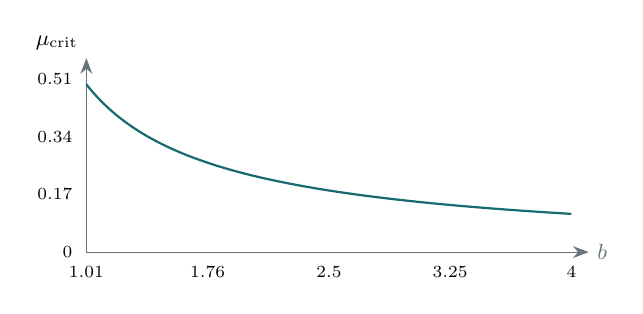
\begin{tikzpicture}[scale=.88,transform shape]
\draw[axis] (0,0.0000000)--(7.25,0.0000000) node[right] {$b$};
\draw[axis] (0.0000000,0)--(0.0000000,2.8);
\node[above left] at (0.0000000,2.8) {$\mu_{\rm crit}$};
\node[below,font=\scriptsize] at (0.0000000,-0.0800000) {$1.01$};
\node[below,font=\scriptsize] at (1.7500000,-0.0800000) {$1.76$};
\node[below,font=\scriptsize] at (3.5000000,-0.0800000) {$2.5$};
\node[below,font=\scriptsize] at (5.2500000,-0.0800000) {$3.25$};
\node[below,font=\scriptsize] at (7.0000000,-0.0800000) {$4$};
\node[left,font=\scriptsize] at (-0.0800000,0.0000000) {$0$};
\node[left,font=\scriptsize] at (-0.0800000,0.8333333) {$0.17$};
\node[left,font=\scriptsize] at (-0.0800000,1.6666667) {$0.34$};
\node[left,font=\scriptsize] at (-0.0800000,2.5000000) {$0.51$};
\draw[thick,color=accent] plot coordinates {(0.0000000,2.4207583) (0.0291667,2.3842309) (0.0583333,2.3488899) (0.0875000,2.3146747) (0.1166667,2.2815288) (0.1458333,2.2493995) (0.1750000,2.2182379) (0.2041667,2.1879980) (0.2333333,2.1586372) (0.2625000,2.1301153) (0.2916667,2.1023947) (0.3208333,2.0754402) (0.3500000,2.0492185) (0.3791667,2.0236985) (0.4083333,1.9988508) (0.4375000,1.9746478) (0.4666667,1.9510633) (0.4958333,1.9280726) (0.5250000,1.9056524) (0.5541667,1.8837806) (0.5833333,1.8624364) (0.6125000,1.8415999) (0.6416667,1.8212523) (0.6708333,1.8013758) (0.7000000,1.7819534) (0.7291667,1.7629690) (0.7583333,1.7444072) (0.7875000,1.7262536) (0.8166667,1.7084940) (0.8458333,1.6911153) (0.8750000,1.6741048) (0.9041667,1.6574504) (0.9333333,1.6411407) (0.9625000,1.6251644) (0.9916667,1.6095112) (1.0208333,1.5941709) (1.0500000,1.5791338) (1.0791667,1.5643907) (1.1083333,1.5499327) (1.1375000,1.5357513) (1.1666667,1.5218383) (1.1958333,1.5081859) (1.2250000,1.4947866) (1.2541667,1.4816332) (1.2833333,1.4687186) (1.3125000,1.4560363) (1.3416667,1.4435798) (1.3708333,1.4313428) (1.4000000,1.4193196) (1.4291667,1.4075042) (1.4583333,1.3958913) (1.4875000,1.3844754) (1.5166667,1.3732514) (1.5458333,1.3622145) (1.5750000,1.3513597) (1.6041667,1.3406825) (1.6333333,1.3301785) (1.6625000,1.3198433) (1.6916667,1.3096727) (1.7208333,1.2996628) (1.7500000,1.2898097) (1.7791667,1.2801095) (1.8083333,1.2705587) (1.8375000,1.2611538) (1.8666667,1.2518913) (1.8958333,1.2427679) (1.9250000,1.2337805) (1.9541667,1.2249259) (1.9833333,1.2162012) (2.0125000,1.2076034) (2.0416667,1.1991297) (2.0708333,1.1907774) (2.1000000,1.1825438) (2.1291667,1.1744264) (2.1583333,1.1664226) (2.1875000,1.1585300) (2.2166667,1.1507463) (2.2458333,1.1430691) (2.2750000,1.1354963) (2.3041667,1.1280257) (2.3333333,1.1206552) (2.3625000,1.1133826) (2.3916667,1.1062062) (2.4208333,1.0991239) (2.4500000,1.0921338) (2.4791667,1.0852341) (2.5083333,1.0784230) (2.5375000,1.0716989) (2.5666667,1.0650599) (2.5958333,1.0585045) (2.6250000,1.0520311) (2.6541667,1.0456381) (2.6833333,1.0393240) (2.7125000,1.0330873) (2.7416667,1.0269266) (2.7708333,1.0208404) (2.8000000,1.0148274) (2.8291667,1.0088862) (2.8583333,1.0030156) (2.8875000,0.9972143) (2.9166667,0.9914810) (2.9458333,0.9858145) (2.9750000,0.9802137) (3.0041667,0.9746774) (3.0333333,0.9692044) (3.0625000,0.9637937) (3.0916667,0.9584441) (3.1208333,0.9531547) (3.1500000,0.9479244) (3.1791667,0.9427522) (3.2083333,0.9376371) (3.2375000,0.9325782) (3.2666667,0.9275745) (3.2958333,0.9226252) (3.3250000,0.9177292) (3.3541667,0.9128859) (3.3833333,0.9080942) (3.4125000,0.9033534) (3.4416667,0.8986626) (3.4708333,0.8940211) (3.5000000,0.8894280) (3.5291667,0.8848826) (3.5583333,0.8803842) (3.5875000,0.8759320) (3.6166667,0.8715252) (3.6458333,0.8671633) (3.6750000,0.8628454) (3.7041667,0.8585710) (3.7333333,0.8543393) (3.7625000,0.8501498) (3.7916667,0.8460017) (3.8208333,0.8418945) (3.8500000,0.8378276) (3.8791667,0.8338002) (3.9083333,0.8298120) (3.9375000,0.8258623) (3.9666667,0.8219505) (3.9958333,0.8180760) (4.0250000,0.8142384) (4.0541667,0.8104372) (4.0833333,0.8066717) (4.1125000,0.8029415) (4.1416667,0.7992461) (4.1708333,0.7955850) (4.2000000,0.7919577) (4.2291667,0.7883637) (4.2583333,0.7848026) (4.2875000,0.7812740) (4.3166667,0.7777773) (4.3458333,0.7743121) (4.3750000,0.7708781) (4.4041667,0.7674747) (4.4333333,0.7641017) (4.4625000,0.7607584) (4.4916667,0.7574447) (4.5208333,0.7541600) (4.5500000,0.7509041) (4.5791667,0.7476764) (4.6083333,0.7444767) (4.6375000,0.7413045) (4.6666667,0.7381596) (4.6958333,0.7350415) (4.7250000,0.7319500) (4.7541667,0.7288846) (4.7833333,0.7258451) (4.8125000,0.7228310) (4.8416667,0.7198422) (4.8708333,0.7168782) (4.9000000,0.7139389) (4.9291667,0.7110237) (4.9583333,0.7081325) (4.9875000,0.7052650) (5.0166667,0.7024208) (5.0458333,0.6995997) (5.0750000,0.6968014) (5.1041667,0.6940256) (5.1333333,0.6912721) (5.1625000,0.6885405) (5.1916667,0.6858306) (5.2208333,0.6831422) (5.2500000,0.6804750) (5.2791667,0.6778287) (5.3083333,0.6752031) (5.3375000,0.6725980) (5.3666667,0.6700131) (5.3958333,0.6674481) (5.4250000,0.6649029) (5.4541667,0.6623772) (5.4833333,0.6598708) (5.5125000,0.6573834) (5.5416667,0.6549149) (5.5708333,0.6524650) (5.6000000,0.6500336) (5.6291667,0.6476203) (5.6583333,0.6452251) (5.6875000,0.6428476) (5.7166667,0.6404878) (5.7458333,0.6381453) (5.7750000,0.6358201) (5.8041667,0.6335119) (5.8333333,0.6312205) (5.8625000,0.6289458) (5.8916667,0.6266876) (5.9208333,0.6244456) (5.9500000,0.6222197) (5.9791667,0.6200098) (6.0083333,0.6178157) (6.0375000,0.6156371) (6.0666667,0.6134740) (6.0958333,0.6113261) (6.1250000,0.6091934) (6.1541667,0.6070755) (6.1833333,0.6049725) (6.2125000,0.6028841) (6.2416667,0.6008102) (6.2708333,0.5987505) (6.3000000,0.5967051) (6.3291667,0.5946737) (6.3583333,0.5926562) (6.3875000,0.5906524) (6.4166667,0.5886622) (6.4458333,0.5866855) (6.4750000,0.5847221) (6.5041667,0.5827719) (6.5333333,0.5808347) (6.5625000,0.5789105) (6.5916667,0.5769991) (6.6208333,0.5751003) (6.6500000,0.5732141) (6.6791667,0.5713403) (6.7083333,0.5694787) (6.7375000,0.5676294) (6.7666667,0.5657921) (6.7958333,0.5639667) (6.8250000,0.5621532) (6.8541667,0.5603513) (6.8833333,0.5585611) (6.9125000,0.5567823) (6.9416667,0.5550149) (6.9708333,0.5532587) (7.0000000,0.5515137)};
\end{tikzpicture}
\figcaption{变图综一.1V8\quad 外半径增大时同步所需的内摩擦比值降低}
\end{minipage}\end{center}
变图综一.1V8画保持初始同步所需的内摩擦系数。地面滑动时$a=\mu_0g$，同步角加速度为$2\mu_0g/(bR)$，内盘所需$f_1=\mu_0mg/b$。于是
\[
\mu_{\rm crit}(b)=\frac{\mu_0}{\sqrt{b^2+(b^2-1)\mu_0^2}}.
\]
较大的外半径降低同步所需的内摩擦比值。取$b=2$即回到本题；终速的$2/3$则来自均匀整盘的总惯量与总质量之间的固定关系。
\end{enumerate}

\Needspace{13\baselineskip}

\pdfbookmark[2]{第 2 题 椭圆轨道的引力规律与彗星速度}{q2}

\section*{第 2 题\quad 椭圆轨道的引力规律与彗星速度}\label{q:2}


一小天体在指向固定太阳的中心力作用下沿非圆椭圆运动，椭圆长、短半轴分别为$A>B>0$，力的大小为$F=GMm/r^\alpha$，比例系数的量纲随$\alpha$取值相应确定。
\begin{enumerate}
\item 若太阳位于（a）椭圆中心，（b）椭圆一个焦点，分别求$\alpha$。除必要条件外，还应说明对应的力确可产生整条椭圆。
\item 在平方反比引力下：（a）求近日点速度及轨道周期；（b）利用图中的彗星绕木星轨道和时间标记，估算近木点速度。图为测量示意，长轴与短轴的纸面长度约为$5.6\,\mathrm{cm}$和$0.30\,\mathrm{cm}$，比例尺$3.5\,\mathrm{cm}$对应$3.0\times10^7\,\mathrm{km}$；1993年7月1日约在远木点，1994年7月16日接近近木端。可把这一时间间隔粗取$380\,\mathrm d$。
\end{enumerate}
讨论把形式近木点速度直接当作进入大气层速度的条件。另取大气入口距木星中心$r_{\rm atm}=7.1\times10^4\,\mathrm{km}$，按同一轨道模型估算该处速度。忽略太阳扰动及大气阻力；一天取$86400\,\mathrm s$。


\begin{center}\begin{minipage}{.98\linewidth}\centering
\begin{tikzpicture}[scale=.8,transform shape]

\draw[object] (0,0) ellipse (2 and 1);
\fill (0,0) circle (2pt) node[below] {中心力心};
\draw[axis] (-2.4,0)--(2.4,0);
\draw[axis] (0,-1.4)--(0,1.4);
\node at (0,2) {（a）};
\begin{scope}[xshift=6cm]
\draw[object] (0,0) ellipse (2 and 1);
\fill (-1.732,0) circle (2pt) node[below] {焦点力心};
\draw[axis] (-2.4,0)--(2.4,0);
\node at (0,2) {（b）};
\end{scope}
\begin{scope}[yshift=-4cm,xshift=3cm,rotate=-20]
\draw[object] (0,0) ellipse (2.8 and .15);
\fill (-2.795979,0) circle (2pt);
\node[above left,rotate=0] at (-2.8,0) {木星、近木端：1994.7.16};
\node[below right,rotate=0] at (2.8,0) {远木端：1993.7.1};
\end{scope}
\draw[axis,<->] (0,-6)--(3.5,-6);
\foreach \x/\s in {0/0,1.1667/10,2.3333/20,3.5/30}{\draw (\x,-5.85)--(\x,-6.15) node[below] {$\s$};}
\node[right] at (4,-6) {$10^6\,\mathrm{km}$};

\end{tikzpicture}
\figcaption{图综一.2\quad 两种力心位置与彗星的极扁轨道测量示意。}
\end{minipage}\end{center}

\Needspace{8\baselineskip}

\pdfbookmark[3]{题型定位}{q2-h0}

\subsection*{题型定位}

中心力轨道的逆问题与天体速度估算。先用端点曲率和角动量确定力的幂指数，再以整条轨道的运动方程说明椭圆确实可实现；周期由面积速度推导。彗星问题把读图、日期间隔、形式近点和大气入口依次联系，速度的大小与所取位置同时给出。

\Needspace{8\baselineskip}

\pdfbookmark[3]{知识点}{q2-h1}

\subsection*{知识点}

\begin{itemize}
\item 椭圆参数式、任一点曲率半径和轴端法向加速度。
\item 中心力角动量守恒，面积速度为$h/2$。
\item 中心线性回复力的正交简谐运动，焦点平方反比力的比耐方程。
\item 半通径$p=B^2/A$、离心率$e=C/A$、端点速度与周期。
\item 同比例尺读图、半周期日期、稳定计算$r_-=B^2/(A+C)$以及不同半径处的机械能关系。
\end{itemize}

\Needspace{8\baselineskip}

\pdfbookmark[3]{物理图像}{q2-h2}

\subsection*{物理图像}

解图综一.2A分别画中心和焦点力心；$P,Q$的力心距离与曲率半径各自标出。图B保留同一比例尺与远近端的时间信息，长短轴按同一长度比例绘制。图C的实线由给定椭圆方程取点，入口$J$是同一轨道与入口圆的交点，形式近点$P_-$在圆内。图D沿轨道半径画真空速度，入口对应横坐标$r/r_{\rm atm}=1$；形式近点对应约$0.50$，位于图示区间的左侧。

\Needspace{8\baselineskip}

\pdfbookmark[3]{解题入口}{q2-h3}

\subsection*{解题入口}

选速度垂直力心半径的轴端，分别写法向运动方程，再以角动量消去速度比。得到指数后，中心情形用参数解，焦点情形用比耐方程，说明全轨道运动。周期从椭圆面积和面积速度之比求出。读图得到$A,B,T$后，先定位形式近点与入口圆，再由机械能式求入口速度。

\Needspace{8\baselineskip}

\pdfbookmark[3]{标准解法}{q2-h4}

\subsection*{标准解法}


图综一.2区分力心位于椭圆中心与焦点的两种几何关系。记焦距
$C=\sqrt{A^2-B^2}$。椭圆长轴端的曲率半径为$B^2/A$，短轴端为$A^2/B$。
\begin{center}\begin{minipage}{.98\linewidth}\centering
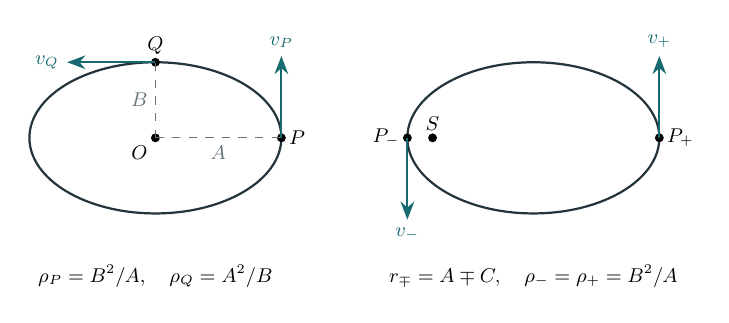
\begin{tikzpicture}[scale=.8,transform shape]

\draw[object] (0,0) ellipse (2 and 1.2);
\fill (0,0) circle (2pt) node[below left] {$O$};
\fill (2,0) circle (2pt) node[right] {$P$};
\fill (0,1.2) circle (2pt) node[above] {$Q$};
\draw[guide] (0,0)--(2,0) node[midway,below] {$A$};
\draw[guide] (0,0)--(0,1.2) node[midway,left] {$B$};
\draw[motion] (2,0)--(2,1.3) node[above] {$v_P$};
\draw[motion] (0,1.2)--(-1.4,1.2) node[left] {$v_Q$};
\node at (0,-2.2) {$\rho_P=B^2/A,\quad\rho_Q=A^2/B$};
\begin{scope}[xshift=6cm]
\draw[object] (0,0) ellipse (2 and 1.2);
\fill (-1.6,0) circle (2pt) node[above] {$S$};
\fill (-2,0) circle (2pt) node[left] {$P_-$};
\fill (2,0) circle (2pt) node[right] {$P_+$};
\draw[motion] (-2,0)--(-2,-1.3) node[below] {$v_-$};
\draw[motion] (2,0)--(2,1.3) node[above] {$v_+$};
\node at (0,-2.2) {$r_\mp=A\mp C,\quad\rho_-=\rho_+=B^2/A$};
\end{scope}

\end{tikzpicture}
\figcaption{解图综一.2A\quad 中心与焦点两种端点比较；力心距离不等同于曲率半径。}
\end{minipage}\end{center}
曲率半径可直接从椭圆参数式推得。令$x=A\cos\phi,y=B\sin\phi$，几何曲率为
\[
\frac1\rho=\frac{|x'y''-y'x''|}{(x'^2+y'^2)^{3/2}}
=\frac{AB}{(A^2\sin^2\phi+B^2\cos^2\phi)^{3/2}}.
\]
在长轴端$\phi=0,\pi$得到$\rho=B^2/A$，短轴端$\phi=\pi/2$得到$\rho=A^2/B$。以中心$O$为力心时，图A中长轴端$P$和短轴端$Q$的切线均垂直于对应的力心半径；以焦点$S$为力心时，选两个长轴端$P_-,P_+$也有这一关系。因此在各自选定的端点，引力完全是法向力，可直接写成$v^2/\rho$。曲线其余位置的法向方向随轨道改变，轴端比较正好避开了切向分量。

解图综一.2A先比较中心力心情形的长轴端$P$和短轴端$Q$。力对中心无力矩，故
\[
Av_P=Bv_Q,\qquad \frac{v_P}{v_Q}=\frac BA.
\]
端点比较中的两个速度由同一守恒量联系。中心力的力矩为零，$m\boldsymbol r\times\boldsymbol v$保持不变；在图A的$P,Q$处，力臂分别为$A,B$，故角动量的大小分别为$mAv_P,mBv_Q$。相除时速度平方比贡献$B^2/A^2$，曲率半径比贡献$A^3/B^3$，最终只剩$A/B$。长短轴不等保证两个不同半径提供独立的幂律信息。

两端速度均垂直于半径，引力完全提供法向加速度：
\[
\frac{GM}{A^\alpha}=\frac{v_P^2}{B^2/A},\qquad
\frac{GM}{B^\alpha}=\frac{v_Q^2}{A^2/B}.
\]
两式相除得
\[
\left(\frac BA\right)^\alpha
=\left(\frac{v_P}{v_Q}\right)^2\frac{A^3}{B^3}
=\frac AB.
\]
因为$A\ne B$，所以$\boxed{\alpha=-1}$。整条椭圆可用参数式表示，取
$x=A\cos nt,y=B\sin nt$，则$\ddot{\boldsymbol r}=-n^2\boldsymbol r$，确为指向中心、大小正比于$r$的力，整条椭圆均满足运动方程。

力心在左焦点$S$时，近日点$P_-$与远日点$P_+$距离分别为$A-C,A+C$，两点曲率半径相同，都是$B^2/A$。角动量守恒给
\[
(A-C)v_-=(A+C)v_+.
\]
两点的法向运动方程相除：
\[
\left(\frac{A+C}{A-C}\right)^\alpha
=\left(\frac{v_-}{v_+}\right)^2
=\left(\frac{A+C}{A-C}\right)^2,
\]
得$\boxed{\alpha=2}$。将运动方程推广到整条轨道，记单位质量角动量$h=r^2\dot\theta$、$u=1/r$，平方反比力的比耐方程为
\[
u''+u=\frac{GM}{h^2}.
\]
比耐方程也可从径向运动逐步导出。以焦点为极点，中心力使$h=r^2\dot\theta$为常量，设$u=1/r$，则
\[
\dot r=-h u',\qquad \ddot r=-h^2u^2u'',\qquad
\ddot r-r\dot\theta^2=-h^2u^2(u''+u).
\]
径向方程右端为$-GM/r^2=-GMu^2$，约去公共因子后得到上述比耐方程。其解中的$p$是半通径，几何关系为$p=B^2/A=A(1-e^2)$，$e=C/A$。在$\theta=0,\pi$时，半径分别为$p/(1+e)=A-C$和$p/(1-e)=A+C$，因而整条极坐标解与题给椭圆的焦点、两轴及端点一致。

其椭圆解$u=(1+e\cos\theta)/p$，其中$p=h^2/(GM)$、$0<e<1$，力心正是焦点。这给出整条椭圆的运动方程。非圆轨道提供两个不同的力心距离；单一圆轨道则给出一个半径处的力。

第（2a）问，以下均取焦点平方反比引力。由近日点的法向方程，
\[
\frac{GM}{(A-C)^2}=\frac{v_-^2}{B^2/A},
\]
得到
\[
\boxed{v_-=\frac B{A-C}\sqrt{\frac{GM}{A}}
=\frac{A+C}{B}\sqrt{\frac{GM}{A}}}.
\]
两种写法由$B^2=(A-C)(A+C)$互换。面积速度恒定，其值可在近日点计算：
\[
\dot{\mathcal A}=\frac12(A-C)v_-=\frac B2\sqrt{\frac{GM}{A}}.
\]
面积速度在任意位置都等于角动量除以$2m$，用近日点是因为该处速度与半径垂直。扫过完整椭圆所需时间等于椭圆面积除以恒定面积速度，所以周期只含半长轴；短半轴既进入面积，也进入面积速度，最终约去。中心力心的线性回复运动则由固定角频率决定周期，同一几何形状在两个力心位置具有不同的时间规律。

椭圆面积为$\pi AB$，故
\[
\boxed{T=\frac{\pi AB}{\dot{\mathcal A}}
=2\pi\sqrt{\frac{A^3}{GM}}}.
\]
\begin{center}\begin{minipage}{.98\linewidth}\centering
\begin{tikzpicture}[scale=.85,transform shape]

\draw[object] (0,0) ellipse (3.8 and .206);
\draw[guide] (-3.8,0)--(3.8,0);
\draw[axis,<->] (-3.8,-1.2)--(3.8,-1.2) node[midway,below] {$2A\simeq4.8\times10^7\,\mathrm{km}$};
\draw[axis,<->] (.7,-.206)--(.7,.206);
\node[above right] at (.7,.206) {$2B\simeq2.6\times10^6\,\mathrm{km}$};
\fill (-3.7944,0) circle (2pt);
\node[above left] at (-3.8,0) {近木端};
\node[above right] at (3.8,0) {远木端};
\node at (0,1.7) {从远木端到近木端约$T/2=380\,\mathrm d$};
\draw[axis,<->] (-3,-3)--(1.75,-3);
\foreach \x/\s in {-3/0,-1.4167/10,.1667/20,1.75/30}{\draw (\x,-2.85)--(\x,-3.15) node[below] {$\s$};}
\node[right] at (2,-3) {$10^6\,\mathrm{km}$};

\end{tikzpicture}
\figcaption{解图综一.2B\quad 读图半轴和时间；轨道长短轴按同一比例绘制。}
\end{minipage}\end{center}
解图综一.2B将轨道长短轴和比例尺放在一起。按题给测量精度，
\[
2A\simeq\frac{5.6}{3.5}(3.0\times10^7)
=4.8\times10^7\,\mathrm{km},
\]
\[
2B\simeq\frac{0.30}{3.5}(3.0\times10^7)
\simeq2.6\times10^6\,\mathrm{km}.
\]
图B的纸面尺寸先由同一标尺换算，再除以2得到半轴。远木端到近木端对应椭圆的一半；两端虽有极大速度差，扫过的面积仍各占半个椭圆，因此所需时间也是半周期。日期间隔按题设粗取$380$天，整周期为$760$天。求引力参数时统一换成米和秒，速度最后再换成千米每秒。短轴的纸面测量仅约$0.30$厘米，读图误差对近点位置和形式近点速度都有明显影响，估算结果用两位有效数字表达。

因此取$A=2.4\times10^7\,\mathrm{km}$、$B=1.3\times10^6\,\mathrm{km}$。从远木端到近木端约半个周期，
$T\simeq760\,\mathrm d=6.57\times10^7\,\mathrm s$。
用周期式消去$GM$，不必另查木星质量：
\[
\sqrt{\frac{GM}{A}}=\frac{2\pi A}{T},\qquad
v_-=\frac{2\pi A(A+C)}{BT}.
\]
轨道很扁，$C\simeq A$，于是
\[
\boxed{v_-\simeq\frac{4\pi A^2}{BT}
\simeq8.5\times10^1\,\mathrm{km/s}}.
\]
该值是把木星作为点引力力心、沿形式椭圆一直走到近木点时的速度。大气入口与形式近点的位置由以下半径比较确定：
\[
r_-=A-C=\frac{B^2}{A+C}\simeq3.52\times10^4\,\mathrm{km}
<r_{\rm atm}.
\]
彗星先穿过大气入口圆，再到达形式近木点；$85\,\mathrm{km/s}$对应形式近点，入口速度在入口半径处计算。
\begin{center}\begin{minipage}{.98\linewidth}\centering
\begin{tikzpicture}[scale=.85,transform shape]
\draw[object] (0,0) circle (1.5);
\draw[traj] plot coordinates {(1.7887149,2.7419037) (1.7685073,2.7309724) (1.7483805,2.7200408) (1.7283344,2.7091086) (1.7083690,2.6981761) (1.6884844,2.6872431) (1.6686805,2.6763097) (1.6489574,2.6653758) (1.6293150,2.6544416) (1.6097533,2.6435069) (1.5902724,2.6325717) (1.5708723,2.6216362) (1.5515529,2.6107002) (1.5323142,2.5997639) (1.5131564,2.5888271) (1.4940793,2.5778899) (1.4750829,2.5669522) (1.4561673,2.5560142) (1.4373325,2.5450758) (1.4185785,2.5341369) (1.3999053,2.5231977) (1.3813128,2.5122580) (1.3628012,2.5013179) (1.3443703,2.4903775) (1.3260202,2.4794366) (1.3077509,2.4684954) (1.2895624,2.4575537) (1.2714548,2.4466117) (1.2534279,2.4356692) (1.2354818,2.4247264) (1.2176165,2.4137832) (1.1998321,2.4028396) (1.1821284,2.3918956) (1.1645056,2.3809513) (1.1469636,2.3700065) (1.1295024,2.3590614) (1.1121221,2.3481159) (1.0948226,2.3371700) (1.0776039,2.3262237) (1.0604660,2.3152771) (1.0434090,2.3043301) (1.0264329,2.2933828) (1.0095375,2.2824350) (0.9927231,2.2714869) (0.9759894,2.2605385) (0.9593366,2.2495897) (0.9427647,2.2386405) (0.9262736,2.2276909) (0.9098634,2.2167410) (0.8935341,2.2057908) (0.8772856,2.1948402) (0.8611180,2.1838892) (0.8450312,2.1729379) (0.8290254,2.1619863) (0.8131004,2.1510343) (0.7972562,2.1400819) (0.7814930,2.1291293) (0.7658106,2.1181762) (0.7502092,2.1072229) (0.7346886,2.0962692) (0.7192489,2.0853151) (0.7038901,2.0743608) (0.6886122,2.0634061) (0.6734152,2.0524510) (0.6582991,2.0414957) (0.6432638,2.0305400) (0.6283095,2.0195840) (0.6134361,2.0086276) (0.5986437,1.9976710) (0.5839321,1.9867140) (0.5693014,1.9757567) (0.5547517,1.9647991) (0.5402829,1.9538412) (0.5258949,1.9428829) (0.5115880,1.9319244) (0.4973619,1.9209655) (0.4832168,1.9100064) (0.4691526,1.8990469) (0.4551693,1.8880871) (0.4412670,1.8771270) (0.4274456,1.8661667) (0.4137051,1.8552060) (0.4000456,1.8442450) (0.3864671,1.8332838) (0.3729694,1.8223222) (0.3595528,1.8113603) (0.3462170,1.8003982) (0.3329623,1.7894358) (0.3197885,1.7784731) (0.3066956,1.7675101) (0.2936837,1.7565468) (0.2807528,1.7455832) (0.2679028,1.7346194) (0.2551338,1.7236552) (0.2424457,1.7126908) (0.2298386,1.7017262) (0.2173125,1.6907612) (0.2048674,1.6797960) (0.1925032,1.6688305) (0.1802201,1.6578648) (0.1680178,1.6468988) (0.1558966,1.6359325) (0.1438564,1.6249660) (0.1318971,1.6139992) (0.1200189,1.6030321) (0.1082216,1.5920648) (0.0965053,1.5810972) (0.0848700,1.5701294) (0.0733157,1.5591613) (0.0618424,1.5481930) (0.0504501,1.5372244) (0.0391388,1.5262556) (0.0279084,1.5152865) (0.0167591,1.5043172) (0.0056908,1.4933477) (-0.0052965,1.4823779) (-0.0162027,1.4714079) (-0.0270280,1.4604376) (-0.0377723,1.4494671) (-0.0484355,1.4384964) (-0.0590178,1.4275255) (-0.0695190,1.4165543) (-0.0799392,1.4055829) (-0.0902784,1.3946113) (-0.1005365,1.3836394) (-0.1107137,1.3726673) (-0.1208098,1.3616950) (-0.1308248,1.3507225) (-0.1407589,1.3397498) (-0.1506119,1.3287768) (-0.1603839,1.3178037) (-0.1700749,1.3068303) (-0.1796848,1.2958567) (-0.1892137,1.2848830) (-0.1986615,1.2739090) (-0.2080283,1.2629348) (-0.2173141,1.2519604) (-0.2265188,1.2409858) (-0.2356425,1.2300110) (-0.2446851,1.2190360) (-0.2536467,1.2080608) (-0.2625273,1.1970854) (-0.2713267,1.1861099) (-0.2800452,1.1751341) (-0.2886826,1.1641582) (-0.2972389,1.1531820) (-0.3057142,1.1422057) (-0.3141084,1.1312292) (-0.3224216,1.1202525) (-0.3306537,1.1092757) (-0.3388047,1.0982986) (-0.3468747,1.0873214) (-0.3548636,1.0763440) (-0.3627715,1.0653664) (-0.3705983,1.0543887) (-0.3783440,1.0434108) (-0.3860086,1.0324327) (-0.3935922,1.0214545) (-0.4010947,1.0104761) (-0.4085162,0.9994976) (-0.4158565,0.9885188) (-0.4231158,0.9775400) (-0.4302941,0.9665609) (-0.4373912,0.9555817) (-0.4444073,0.9446024) (-0.4513422,0.9336229) (-0.4581962,0.9226433) (-0.4649690,0.9116635) (-0.4716607,0.9006836) (-0.4782714,0.8897035) (-0.4848010,0.8787233) (-0.4912494,0.8677429) (-0.4976169,0.8567624) (-0.5039032,0.8457818) (-0.5101084,0.8348010) (-0.5162325,0.8238201) (-0.5222756,0.8128390) (-0.5282375,0.8018579) (-0.5341184,0.7908766) (-0.5399182,0.7798952) (-0.5456369,0.7689136) (-0.5512744,0.7579319) (-0.5568309,0.7469501) (-0.5623063,0.7359682) (-0.5677006,0.7249862) (-0.5730138,0.7140041) (-0.5782459,0.7030218) (-0.5833969,0.6920394) (-0.5884668,0.6810569) (-0.5934556,0.6700744) (-0.5983633,0.6590917) (-0.6031899,0.6481088) (-0.6079353,0.6371259) (-0.6125997,0.6261429) (-0.6171830,0.6151598) (-0.6216852,0.6041766) (-0.6261062,0.5931933) (-0.6304462,0.5822099) (-0.6347050,0.5712264) (-0.6388827,0.5602428) (-0.6429794,0.5492592) (-0.6469949,0.5382754) (-0.6509293,0.5272915) (-0.6547826,0.5163076) (-0.6585547,0.5053236) (-0.6622458,0.4943395) (-0.6658558,0.4833553) (-0.6693846,0.4723711) (-0.6728323,0.4613867) (-0.6761989,0.4504023) (-0.6794844,0.4394179) (-0.6826888,0.4284333) (-0.6858120,0.4174487) (-0.6888542,0.4064640) (-0.6918152,0.3954793) (-0.6946951,0.3844945) (-0.6974939,0.3735096) (-0.7002116,0.3625247) (-0.7028481,0.3515397) (-0.7054035,0.3405547) (-0.7078778,0.3295696) (-0.7102710,0.3185844) (-0.7125831,0.3075992) (-0.7148140,0.2966140) (-0.7169638,0.2856287) (-0.7190325,0.2746433) (-0.7210201,0.2636579) (-0.7229266,0.2526725) (-0.7247519,0.2416870) (-0.7264961,0.2307015) (-0.7281592,0.2197160) (-0.7297411,0.2087304) (-0.7312420,0.1977448) (-0.7326617,0.1867591) (-0.7340003,0.1757734) (-0.7352577,0.1647877) (-0.7364340,0.1538020) (-0.7375292,0.1428163) (-0.7385433,0.1318305) (-0.7394763,0.1208447) (-0.7403281,0.1098589) (-0.7410988,0.0988730) (-0.7417884,0.0878872) (-0.7423968,0.0769013) (-0.7429242,0.0659154) (-0.7433704,0.0549295) (-0.7437354,0.0439436) (-0.7440194,0.0329577) (-0.7442222,0.0219718) (-0.7443439,0.0109859) (-0.7443844,0.0000000) (-0.7443439,-0.0109859) (-0.7442222,-0.0219718) (-0.7440194,-0.0329577) (-0.7437354,-0.0439436) (-0.7433704,-0.0549295) (-0.7429242,-0.0659154) (-0.7423968,-0.0769013) (-0.7417884,-0.0878872) (-0.7410988,-0.0988730) (-0.7403281,-0.1098589) (-0.7394763,-0.1208447) (-0.7385433,-0.1318305) (-0.7375292,-0.1428163) (-0.7364340,-0.1538020) (-0.7352577,-0.1647877) (-0.7340003,-0.1757734) (-0.7326617,-0.1867591) (-0.7312420,-0.1977448) (-0.7297411,-0.2087304) (-0.7281592,-0.2197160) (-0.7264961,-0.2307015) (-0.7247519,-0.2416870) (-0.7229266,-0.2526725) (-0.7210201,-0.2636579) (-0.7190325,-0.2746433) (-0.7169638,-0.2856287) (-0.7148140,-0.2966140) (-0.7125831,-0.3075992) (-0.7102710,-0.3185844) (-0.7078778,-0.3295696) (-0.7054035,-0.3405547) (-0.7028481,-0.3515397) (-0.7002116,-0.3625247) (-0.6974939,-0.3735096) (-0.6946951,-0.3844945) (-0.6918152,-0.3954793) (-0.6888542,-0.4064640) (-0.6858120,-0.4174487) (-0.6826888,-0.4284333) (-0.6794844,-0.4394179) (-0.6761989,-0.4504023) (-0.6728323,-0.4613867) (-0.6693846,-0.4723711) (-0.6658558,-0.4833553) (-0.6622458,-0.4943395) (-0.6585547,-0.5053236) (-0.6547826,-0.5163076) (-0.6509293,-0.5272915) (-0.6469949,-0.5382754) (-0.6429794,-0.5492592) (-0.6388827,-0.5602428) (-0.6347050,-0.5712264) (-0.6304462,-0.5822099) (-0.6261062,-0.5931933) (-0.6216852,-0.6041766) (-0.6171830,-0.6151598) (-0.6125997,-0.6261429) (-0.6079353,-0.6371259) (-0.6031899,-0.6481088) (-0.5983633,-0.6590917) (-0.5934556,-0.6700744) (-0.5884668,-0.6810569) (-0.5833969,-0.6920394) (-0.5782459,-0.7030218) (-0.5730138,-0.7140041) (-0.5677006,-0.7249862) (-0.5623063,-0.7359682) (-0.5568309,-0.7469501) (-0.5512744,-0.7579319) (-0.5456369,-0.7689136) (-0.5399182,-0.7798952) (-0.5341184,-0.7908766) (-0.5282375,-0.8018579) (-0.5222756,-0.8128390) (-0.5162325,-0.8238201) (-0.5101084,-0.8348010) (-0.5039032,-0.8457818) (-0.4976169,-0.8567624) (-0.4912494,-0.8677429) (-0.4848010,-0.8787233) (-0.4782714,-0.8897035) (-0.4716607,-0.9006836) (-0.4649690,-0.9116635) (-0.4581962,-0.9226433) (-0.4513422,-0.9336229) (-0.4444073,-0.9446024) (-0.4373912,-0.9555817) (-0.4302941,-0.9665609) (-0.4231158,-0.9775400) (-0.4158565,-0.9885188) (-0.4085162,-0.9994976) (-0.4010947,-1.0104761) (-0.3935922,-1.0214545) (-0.3860086,-1.0324327) (-0.3783440,-1.0434108) (-0.3705983,-1.0543887) (-0.3627715,-1.0653664) (-0.3548636,-1.0763440) (-0.3468747,-1.0873214) (-0.3388047,-1.0982986) (-0.3306537,-1.1092757) (-0.3224216,-1.1202525) (-0.3141084,-1.1312292) (-0.3057142,-1.1422057) (-0.2972389,-1.1531820) (-0.2886826,-1.1641582) (-0.2800452,-1.1751341) (-0.2713267,-1.1861099) (-0.2625273,-1.1970854) (-0.2536467,-1.2080608) (-0.2446851,-1.2190360) (-0.2356425,-1.2300110) (-0.2265188,-1.2409858) (-0.2173141,-1.2519604) (-0.2080283,-1.2629348) (-0.1986615,-1.2739090) (-0.1892137,-1.2848830) (-0.1796848,-1.2958567) (-0.1700749,-1.3068303) (-0.1603839,-1.3178037) (-0.1506119,-1.3287768) (-0.1407589,-1.3397498) (-0.1308248,-1.3507225) (-0.1208098,-1.3616950) (-0.1107137,-1.3726673) (-0.1005365,-1.3836394) (-0.0902784,-1.3946113) (-0.0799392,-1.4055829) (-0.0695190,-1.4165543) (-0.0590178,-1.4275255) (-0.0484355,-1.4384964) (-0.0377723,-1.4494671) (-0.0270280,-1.4604376) (-0.0162027,-1.4714079) (-0.0052965,-1.4823779) (0.0056908,-1.4933477) (0.0167591,-1.5043172) (0.0279084,-1.5152865) (0.0391388,-1.5262556) (0.0504501,-1.5372244) (0.0618424,-1.5481930) (0.0733157,-1.5591613) (0.0848700,-1.5701294) (0.0965053,-1.5810972) (0.1082216,-1.5920648) (0.1200189,-1.6030321) (0.1318971,-1.6139992) (0.1438564,-1.6249660) (0.1558966,-1.6359325) (0.1680178,-1.6468988) (0.1802201,-1.6578648) (0.1925032,-1.6688305) (0.2048674,-1.6797960) (0.2173125,-1.6907612) (0.2298386,-1.7017262) (0.2424457,-1.7126908) (0.2551338,-1.7236552) (0.2679028,-1.7346194) (0.2807528,-1.7455832) (0.2936837,-1.7565468) (0.3066956,-1.7675101) (0.3197885,-1.7784731) (0.3329623,-1.7894358) (0.3462170,-1.8003982) (0.3595528,-1.8113603) (0.3729694,-1.8223222) (0.3864671,-1.8332838) (0.4000456,-1.8442450) (0.4137051,-1.8552060) (0.4274456,-1.8661667) (0.4412670,-1.8771270) (0.4551693,-1.8880871) (0.4691526,-1.8990469) (0.4832168,-1.9100064) (0.4973619,-1.9209655) (0.5115880,-1.9319244) (0.5258949,-1.9428829) (0.5402829,-1.9538412) (0.5547517,-1.9647991) (0.5693014,-1.9757567) (0.5839321,-1.9867140) (0.5986437,-1.9976710) (0.6134361,-2.0086276) (0.6283095,-2.0195840) (0.6432638,-2.0305400) (0.6582991,-2.0414957) (0.6734152,-2.0524510) (0.6886122,-2.0634061) (0.7038901,-2.0743608) (0.7192489,-2.0853151) (0.7346886,-2.0962692) (0.7502092,-2.1072229) (0.7658106,-2.1181762) (0.7814930,-2.1291293) (0.7972562,-2.1400819) (0.8131004,-2.1510343) (0.8290254,-2.1619863) (0.8450312,-2.1729379) (0.8611180,-2.1838892) (0.8772856,-2.1948402) (0.8935341,-2.2057908) (0.9098634,-2.2167410) (0.9262736,-2.2276909) (0.9427647,-2.2386405) (0.9593366,-2.2495897) (0.9759894,-2.2605385) (0.9927231,-2.2714869) (1.0095375,-2.2824350) (1.0264329,-2.2933828) (1.0434090,-2.3043301) (1.0604660,-2.3152771) (1.0776039,-2.3262237) (1.0948226,-2.3371700) (1.1121221,-2.3481159) (1.1295024,-2.3590614) (1.1469636,-2.3700065) (1.1645056,-2.3809513) (1.1821284,-2.3918956) (1.1998321,-2.4028396) (1.2176165,-2.4137832) (1.2354818,-2.4247264) (1.2534279,-2.4356692) (1.2714548,-2.4466117) (1.2895624,-2.4575537) (1.3077509,-2.4684954) (1.3260202,-2.4794366) (1.3443703,-2.4903775) (1.3628012,-2.5013179) (1.3813128,-2.5122580) (1.3999053,-2.5231977) (1.4185785,-2.5341369) (1.4373325,-2.5450758) (1.4561673,-2.5560142) (1.4750829,-2.5669522) (1.4940793,-2.5778899) (1.5131564,-2.5888271) (1.5323142,-2.5997639) (1.5515529,-2.6107002) (1.5708723,-2.6216362) (1.5902724,-2.6325717) (1.6097533,-2.6435069) (1.6293150,-2.6544416) (1.6489574,-2.6653758) (1.6686805,-2.6763097) (1.6884844,-2.6872431) (1.7083690,-2.6981761) (1.7283344,-2.7091086) (1.7483805,-2.7200408) (1.7685073,-2.7309724) (1.7887149,-2.7419037)};
\fill (0,0) circle (1.8pt) node[below right] {$S$};
\fill (-0.7443844,0) circle (1.8pt) node[below left] {$P_-$};
\fill (0.0123421,1.4999492) circle (2pt) node[above right] {$J$};
\draw[guide] (0,0)--(0.0123421,1.4999492) node[midway,right] {$r_{\rm atm}$};
\node[align=left,right] at (3,0) {圆心$S$为木星中心\\圆周为大气入口\\实线为同一椭圆的局部\\$P_-$位于圆内};
\end{tikzpicture}
\figcaption{解图综一.2C\quad 入口圆与椭圆的真实交点；横纵采用相同长度比例}
\end{minipage}\end{center}
解图综一.2C中的实线由同一个椭圆方程取点绘成，木星中心为焦点$S$，入口圆半径为$r_{\rm atm}$。曲线在$J$第一次穿过入口圆，形式近点$P_-$位于圆内。入口以后的真实运动还受到大气作用；本题把真空椭圆速度计算到$J$，由该处半径代入机械能式。这样近点速度与入口速度各有明确的几何位置。

解图综一.2C放大木星附近的入口$J$，从机械能守恒求入口处速度。把已求得的近日点速度代入单位质量机械能：
\[
\begin{aligned}
\mathcal E&=\frac{v_-^2}{2}-\frac{GM}{A-C}\\
&=\frac{GM}{A-C}\left(\frac{A+C}{2A}-1\right)
=-\frac{GM}{2A}.
\end{aligned}
\]
所以任一点满足
\[
\frac{v^2}{2}-\frac{GM}{r}=-\frac{GM}{2A},
\qquad v^2=GM\left(\frac2r-\frac1A\right).
\]
同一机械能沿整条真空椭圆保持不变。由周期反算
\[
GM=\frac{4\pi^2A^3}{T^2}
\simeq1.27\times10^{17}\,\mathrm{m^3/s^2},
\]
在$r=r_{\rm atm}=7.1\times10^7\,\mathrm m$处，
\[
\boxed{v_{\rm atm}
=\sqrt{\frac{4\pi^2A^3}{T^2}
\left(\frac2{r_{\rm atm}}-\frac1A\right)}
\simeq6.0\times10^1\,\mathrm{km/s}}.
\]
两项速度对应不同位置。图上轴长、时间和忽略扰动的精度共同决定估算精度，结果保留约两位有效数字。
\begin{center}\begin{minipage}{.98\linewidth}\centering
\begin{tikzpicture}[scale=.88,transform shape]
\draw[axis] (0,0.0000000)--(7.25,0.0000000) node[right] {$r/r_{\rm atm}$};
\draw[axis] (0.0000000,0)--(0.0000000,2.8);
\node[above left] at (0.0000000,2.8) {$v/\sqrt{GM/r_{\rm atm}}$};
\node[below,font=\scriptsize] at (0.0000000,-0.0800000) {$1$};
\node[below,font=\scriptsize] at (1.7500000,-0.0800000) {$1.5$};
\node[below,font=\scriptsize] at (3.5000000,-0.0800000) {$2$};
\node[below,font=\scriptsize] at (5.2500000,-0.0800000) {$2.5$};
\node[below,font=\scriptsize] at (7.0000000,-0.0800000) {$3$};
\node[left,font=\scriptsize] at (-0.0800000,0.0000000) {$0$};
\node[left,font=\scriptsize] at (-0.0800000,0.8333333) {$0.5$};
\node[left,font=\scriptsize] at (-0.0800000,1.6666667) {$1$};
\node[left,font=\scriptsize] at (-0.0800000,2.5000000) {$1.5$};
\draw[thick,color=accent] plot coordinates {(0.0000000,2.3552787) (0.0291667,2.3455115) (0.0583333,2.3358646) (0.0875000,2.3263354) (0.1166667,2.3169218) (0.1458333,2.3076212) (0.1750000,2.2984316) (0.2041667,2.2893506) (0.2333333,2.2803762) (0.2625000,2.2715063) (0.2916667,2.2627389) (0.3208333,2.2540721) (0.3500000,2.2455038) (0.3791667,2.2370324) (0.4083333,2.2286558) (0.4375000,2.2203725) (0.4666667,2.2121806) (0.4958333,2.2040786) (0.5250000,2.1960647) (0.5541667,2.1881374) (0.5833333,2.1802952) (0.6125000,2.1725365) (0.6416667,2.1648598) (0.6708333,2.1572638) (0.7000000,2.1497470) (0.7291667,2.1423080) (0.7583333,2.1349455) (0.7875000,2.1276583) (0.8166667,2.1204450) (0.8458333,2.1133044) (0.8750000,2.1062352) (0.9041667,2.0992364) (0.9333333,2.0923067) (0.9625000,2.0854450) (0.9916667,2.0786502) (1.0208333,2.0719213) (1.0500000,2.0652570) (1.0791667,2.0586566) (1.1083333,2.0521188) (1.1375000,2.0456428) (1.1666667,2.0392276) (1.1958333,2.0328721) (1.2250000,2.0265756) (1.2541667,2.0203371) (1.2833333,2.0141557) (1.3125000,2.0080305) (1.3416667,2.0019607) (1.3708333,1.9959455) (1.4000000,1.9899840) (1.4291667,1.9840755) (1.4583333,1.9782192) (1.4875000,1.9724142) (1.5166667,1.9666600) (1.5458333,1.9609556) (1.5750000,1.9553005) (1.6041667,1.9496939) (1.6333333,1.9441351) (1.6625000,1.9386234) (1.6916667,1.9331582) (1.7208333,1.9277389) (1.7500000,1.9223647) (1.7791667,1.9170351) (1.8083333,1.9117495) (1.8375000,1.9065072) (1.8666667,1.9013077) (1.8958333,1.8961503) (1.9250000,1.8910346) (1.9541667,1.8859599) (1.9833333,1.8809258) (2.0125000,1.8759316) (2.0416667,1.8709768) (2.0708333,1.8660610) (2.1000000,1.8611837) (2.1291667,1.8563442) (2.1583333,1.8515422) (2.1875000,1.8467771) (2.2166667,1.8420486) (2.2458333,1.8373560) (2.2750000,1.8326990) (2.3041667,1.8280772) (2.3333333,1.8234900) (2.3625000,1.8189371) (2.3916667,1.8144179) (2.4208333,1.8099322) (2.4500000,1.8054795) (2.4791667,1.8010594) (2.5083333,1.7966715) (2.5375000,1.7923154) (2.5666667,1.7879907) (2.5958333,1.7836970) (2.6250000,1.7794341) (2.6541667,1.7752014) (2.6833333,1.7709987) (2.7125000,1.7668256) (2.7416667,1.7626818) (2.7708333,1.7585669) (2.8000000,1.7544806) (2.8291667,1.7504225) (2.8583333,1.7463924) (2.8875000,1.7423899) (2.9166667,1.7384146) (2.9458333,1.7344664) (2.9750000,1.7305448) (3.0041667,1.7266497) (3.0333333,1.7227806) (3.0625000,1.7189373) (3.0916667,1.7151195) (3.1208333,1.7113270) (3.1500000,1.7075594) (3.1791667,1.7038165) (3.2083333,1.7000980) (3.2375000,1.6964036) (3.2666667,1.6927332) (3.2958333,1.6890864) (3.3250000,1.6854629) (3.3541667,1.6818626) (3.3833333,1.6782852) (3.4125000,1.6747304) (3.4416667,1.6711980) (3.4708333,1.6676878) (3.5000000,1.6641996) (3.5291667,1.6607330) (3.5583333,1.6572879) (3.5875000,1.6538642) (3.6166667,1.6504614) (3.6458333,1.6470795) (3.6750000,1.6437182) (3.7041667,1.6403773) (3.7333333,1.6370566) (3.7625000,1.6337560) (3.7916667,1.6304751) (3.8208333,1.6272138) (3.8500000,1.6239720) (3.8791667,1.6207494) (3.9083333,1.6175458) (3.9375000,1.6143610) (3.9666667,1.6111949) (3.9958333,1.6080473) (4.0250000,1.6049180) (4.0541667,1.6018068) (4.0833333,1.5987135) (4.1125000,1.5956381) (4.1416667,1.5925802) (4.1708333,1.5895398) (4.2000000,1.5865166) (4.2291667,1.5835106) (4.2583333,1.5805215) (4.2875000,1.5775491) (4.3166667,1.5745935) (4.3458333,1.5716543) (4.3750000,1.5687314) (4.4041667,1.5658247) (4.4333333,1.5629340) (4.4625000,1.5600592) (4.4916667,1.5572002) (4.5208333,1.5543567) (4.5500000,1.5515287) (4.5791667,1.5487160) (4.6083333,1.5459185) (4.6375000,1.5431360) (4.6666667,1.5403684) (4.6958333,1.5376156) (4.7250000,1.5348774) (4.7541667,1.5321537) (4.7833333,1.5294444) (4.8125000,1.5267494) (4.8416667,1.5240685) (4.8708333,1.5214016) (4.9000000,1.5187486) (4.9291667,1.5161093) (4.9583333,1.5134837) (4.9875000,1.5108717) (5.0166667,1.5082730) (5.0458333,1.5056876) (5.0750000,1.5031155) (5.1041667,1.5005564) (5.1333333,1.4980102) (5.1625000,1.4954770) (5.1916667,1.4929564) (5.2208333,1.4904485) (5.2500000,1.4879532) (5.2791667,1.4854702) (5.3083333,1.4829996) (5.3375000,1.4805413) (5.3666667,1.4780950) (5.3958333,1.4756608) (5.4250000,1.4732385) (5.4541667,1.4708280) (5.4833333,1.4684293) (5.5125000,1.4660422) (5.5416667,1.4636666) (5.5708333,1.4613025) (5.6000000,1.4589498) (5.6291667,1.4566083) (5.6583333,1.4542781) (5.6875000,1.4519589) (5.7166667,1.4496507) (5.7458333,1.4473534) (5.7750000,1.4450669) (5.8041667,1.4427912) (5.8333333,1.4405262) (5.8625000,1.4382717) (5.8916667,1.4360278) (5.9208333,1.4337942) (5.9500000,1.4315710) (5.9791667,1.4293581) (6.0083333,1.4271553) (6.0375000,1.4249626) (6.0666667,1.4227799) (6.0958333,1.4206072) (6.1250000,1.4184444) (6.1541667,1.4162913) (6.1833333,1.4141480) (6.2125000,1.4120143) (6.2416667,1.4098902) (6.2708333,1.4077756) (6.3000000,1.4056704) (6.3291667,1.4035746) (6.3583333,1.4014881) (6.3875000,1.3994109) (6.4166667,1.3973427) (6.4458333,1.3952837) (6.4750000,1.3932337) (6.5041667,1.3911927) (6.5333333,1.3891605) (6.5625000,1.3871372) (6.5916667,1.3851226) (6.6208333,1.3831168) (6.6500000,1.3811196) (6.6791667,1.3791309) (6.7083333,1.3771508) (6.7375000,1.3751791) (6.7666667,1.3732159) (6.7958333,1.3712609) (6.8250000,1.3693143) (6.8541667,1.3673758) (6.8833333,1.3654456) (6.9125000,1.3635234) (6.9416667,1.3616093) (6.9708333,1.3597031) (7.0000000,1.3578049)};
\end{tikzpicture}
\figcaption{解图综一.2D\quad 同一真空椭圆上不同半径对应的速度}
\end{minipage}\end{center}
解图综一.2D画$v/\sqrt{GM/r_{\rm atm}}$随$r/r_{\rm atm}$的变化。沿入射支，半径减小，势能降低，速度增加；在入口圆上速度约为$60\ \mathrm{km/s}$。形式近点处约$85\ \mathrm{km/s}$对应更小的半径。若形式近点恰好接近所取入口圆，两数才会接近；本题的两半径相差约一倍，分开代入机械能式可以保留这一几何差异。



\Needspace{8\baselineskip}

\pdfbookmark[3]{关键洞察}{q2-h5}

\subsection*{关键洞察}

同一椭圆以中心或焦点为力心，会对应不同的径向力规律：几何形状和力心位置一起决定动力学。长轴端和短轴端的曲率半径差异提供中心情形的指数信息，焦点情形则利用两个长轴端相同的曲率。极扁轨道中$r_-=B^2/(A+C)$对短轴的平方敏感，读图误差会明显改变形式近点位置。实际入口速度按入口半径计算。

\Needspace{8\baselineskip}

\pdfbookmark[3]{易错点}{q2-h6}

\subsection*{易错点}

\begin{itemize}
\item 力心距离$r$进入引力公式，曲率半径$\rho$进入法向加速度，二者分别使用。
\item 非圆条件$A>B$保证两端给出不同半径的信息；圆轨道只给一个半径处的力。
\item 纸面长短轴换成实际全轴后各除以2，远端到近端的日期间隔再乘以2得到周期。
\item 引力参数计算统一采用米和秒，速度最后换算成千米每秒。
\item 用$B^2/(A+C)$计算很小的近点半径，再确定它与入口圆的位置关系。
\end{itemize}

\Needspace{8\baselineskip}

\pdfbookmark[3]{课堂讲解建议}{q2-h7}

\subsection*{课堂讲解建议}

先用两种颜色标中心与焦点，让学生在同一轴端依次说出力心距离、曲率半径和速度方向。推出指数后问：“两点的方程怎样扩展到整条轨道？”分别由正交简谐运动和比耐方程回答。推周期时让学生指出$B$在面积与面积速度中怎样约去。读图题先收集$85\ \mathrm{km/s}$，再问：“这个数对应轨道上的哪一点？入口圆又在哪里？”学生计算$B^2/(A+C)$，在图C标出$P_-$与$J$，再求入口约$60\ \mathrm{km/s}$。最后追问短轴加倍会怎样，联系变式四解释整个椭圆移到入口圆外侧。

\Needspace{8\baselineskip}

\pdfbookmark[3]{变式训练}{q2-h8}

\subsection*{变式训练}

\begin{enumerate}
\item \textbf{圆轨道能给出多少幂律信息。} 若只知道半径$r_*$的圆轨道速度$v_*$，给定任意指数$\alpha$，求可产生这条轨道的力系数。
\par 写单位质量中心加速度为$-K r^{-\alpha}\hat{\boldsymbol r}$。圆周运动条件给$K=v_*^2r_*^{\alpha-1}$，因而同一条观测圆轨道与任意$\alpha$都相容。其他半径处相应的圆速度为
\[
\frac{v_c(r)}{v_*}=\left(\frac r{r_*}\right)^{(1-\alpha)/2}.
\]
\begin{center}\begin{minipage}{.98\linewidth}\centering
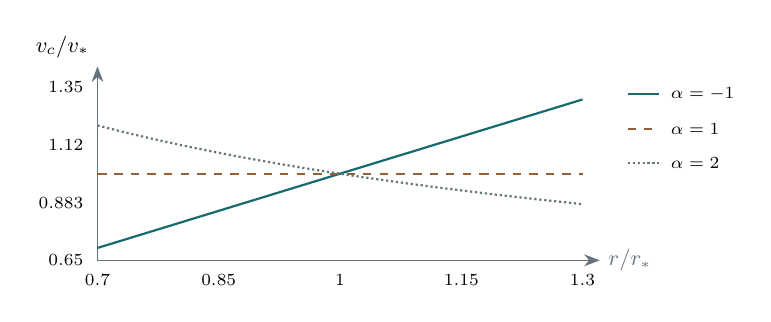
\begin{tikzpicture}[scale=.88,transform shape]
\draw[axis] (0,0.0000000)--(7.25,0.0000000) node[right] {$r/r_*$};
\draw[axis] (0.0000000,0)--(0.0000000,2.8);
\node[above left] at (0.0000000,2.8) {$v_c/v_*$};
\node[below,font=\scriptsize] at (0.0000000,-0.0800000) {$0.7$};
\node[below,font=\scriptsize] at (1.7500000,-0.0800000) {$0.85$};
\node[below,font=\scriptsize] at (3.5000000,-0.0800000) {$1$};
\node[below,font=\scriptsize] at (5.2500000,-0.0800000) {$1.15$};
\node[below,font=\scriptsize] at (7.0000000,-0.0800000) {$1.3$};
\node[left,font=\scriptsize] at (-0.0800000,0.0000000) {$0.65$};
\node[left,font=\scriptsize] at (-0.0800000,0.8333333) {$0.883$};
\node[left,font=\scriptsize] at (-0.0800000,1.6666667) {$1.12$};
\node[left,font=\scriptsize] at (-0.0800000,2.5000000) {$1.35$};
\draw[thick,color=accent] plot coordinates {(0.0000000,0.1785714) (0.0291667,0.1875000) (0.0583333,0.1964286) (0.0875000,0.2053571) (0.1166667,0.2142857) (0.1458333,0.2232143) (0.1750000,0.2321429) (0.2041667,0.2410714) (0.2333333,0.2500000) (0.2625000,0.2589286) (0.2916667,0.2678571) (0.3208333,0.2767857) (0.3500000,0.2857143) (0.3791667,0.2946429) (0.4083333,0.3035714) (0.4375000,0.3125000) (0.4666667,0.3214286) (0.4958333,0.3303571) (0.5250000,0.3392857) (0.5541667,0.3482143) (0.5833333,0.3571429) (0.6125000,0.3660714) (0.6416667,0.3750000) (0.6708333,0.3839286) (0.7000000,0.3928571) (0.7291667,0.4017857) (0.7583333,0.4107143) (0.7875000,0.4196429) (0.8166667,0.4285714) (0.8458333,0.4375000) (0.8750000,0.4464286) (0.9041667,0.4553571) (0.9333333,0.4642857) (0.9625000,0.4732143) (0.9916667,0.4821429) (1.0208333,0.4910714) (1.0500000,0.5000000) (1.0791667,0.5089286) (1.1083333,0.5178571) (1.1375000,0.5267857) (1.1666667,0.5357143) (1.1958333,0.5446429) (1.2250000,0.5535714) (1.2541667,0.5625000) (1.2833333,0.5714286) (1.3125000,0.5803571) (1.3416667,0.5892857) (1.3708333,0.5982143) (1.4000000,0.6071429) (1.4291667,0.6160714) (1.4583333,0.6250000) (1.4875000,0.6339286) (1.5166667,0.6428571) (1.5458333,0.6517857) (1.5750000,0.6607143) (1.6041667,0.6696429) (1.6333333,0.6785714) (1.6625000,0.6875000) (1.6916667,0.6964286) (1.7208333,0.7053571) (1.7500000,0.7142857) (1.7791667,0.7232143) (1.8083333,0.7321429) (1.8375000,0.7410714) (1.8666667,0.7500000) (1.8958333,0.7589286) (1.9250000,0.7678571) (1.9541667,0.7767857) (1.9833333,0.7857143) (2.0125000,0.7946429) (2.0416667,0.8035714) (2.0708333,0.8125000) (2.1000000,0.8214286) (2.1291667,0.8303571) (2.1583333,0.8392857) (2.1875000,0.8482143) (2.2166667,0.8571429) (2.2458333,0.8660714) (2.2750000,0.8750000) (2.3041667,0.8839286) (2.3333333,0.8928571) (2.3625000,0.9017857) (2.3916667,0.9107143) (2.4208333,0.9196429) (2.4500000,0.9285714) (2.4791667,0.9375000) (2.5083333,0.9464286) (2.5375000,0.9553571) (2.5666667,0.9642857) (2.5958333,0.9732143) (2.6250000,0.9821429) (2.6541667,0.9910714) (2.6833333,1.0000000) (2.7125000,1.0089286) (2.7416667,1.0178571) (2.7708333,1.0267857) (2.8000000,1.0357143) (2.8291667,1.0446429) (2.8583333,1.0535714) (2.8875000,1.0625000) (2.9166667,1.0714286) (2.9458333,1.0803571) (2.9750000,1.0892857) (3.0041667,1.0982143) (3.0333333,1.1071429) (3.0625000,1.1160714) (3.0916667,1.1250000) (3.1208333,1.1339286) (3.1500000,1.1428571) (3.1791667,1.1517857) (3.2083333,1.1607143) (3.2375000,1.1696429) (3.2666667,1.1785714) (3.2958333,1.1875000) (3.3250000,1.1964286) (3.3541667,1.2053571) (3.3833333,1.2142857) (3.4125000,1.2232143) (3.4416667,1.2321429) (3.4708333,1.2410714) (3.5000000,1.2500000) (3.5291667,1.2589286) (3.5583333,1.2678571) (3.5875000,1.2767857) (3.6166667,1.2857143) (3.6458333,1.2946429) (3.6750000,1.3035714) (3.7041667,1.3125000) (3.7333333,1.3214286) (3.7625000,1.3303571) (3.7916667,1.3392857) (3.8208333,1.3482143) (3.8500000,1.3571429) (3.8791667,1.3660714) (3.9083333,1.3750000) (3.9375000,1.3839286) (3.9666667,1.3928571) (3.9958333,1.4017857) (4.0250000,1.4107143) (4.0541667,1.4196429) (4.0833333,1.4285714) (4.1125000,1.4375000) (4.1416667,1.4464286) (4.1708333,1.4553571) (4.2000000,1.4642857) (4.2291667,1.4732143) (4.2583333,1.4821429) (4.2875000,1.4910714) (4.3166667,1.5000000) (4.3458333,1.5089286) (4.3750000,1.5178571) (4.4041667,1.5267857) (4.4333333,1.5357143) (4.4625000,1.5446429) (4.4916667,1.5535714) (4.5208333,1.5625000) (4.5500000,1.5714286) (4.5791667,1.5803571) (4.6083333,1.5892857) (4.6375000,1.5982143) (4.6666667,1.6071429) (4.6958333,1.6160714) (4.7250000,1.6250000) (4.7541667,1.6339286) (4.7833333,1.6428571) (4.8125000,1.6517857) (4.8416667,1.6607143) (4.8708333,1.6696429) (4.9000000,1.6785714) (4.9291667,1.6875000) (4.9583333,1.6964286) (4.9875000,1.7053571) (5.0166667,1.7142857) (5.0458333,1.7232143) (5.0750000,1.7321429) (5.1041667,1.7410714) (5.1333333,1.7500000) (5.1625000,1.7589286) (5.1916667,1.7678571) (5.2208333,1.7767857) (5.2500000,1.7857143) (5.2791667,1.7946429) (5.3083333,1.8035714) (5.3375000,1.8125000) (5.3666667,1.8214286) (5.3958333,1.8303571) (5.4250000,1.8392857) (5.4541667,1.8482143) (5.4833333,1.8571429) (5.5125000,1.8660714) (5.5416667,1.8750000) (5.5708333,1.8839286) (5.6000000,1.8928571) (5.6291667,1.9017857) (5.6583333,1.9107143) (5.6875000,1.9196429) (5.7166667,1.9285714) (5.7458333,1.9375000) (5.7750000,1.9464286) (5.8041667,1.9553571) (5.8333333,1.9642857) (5.8625000,1.9732143) (5.8916667,1.9821429) (5.9208333,1.9910714) (5.9500000,2.0000000) (5.9791667,2.0089286) (6.0083333,2.0178571) (6.0375000,2.0267857) (6.0666667,2.0357143) (6.0958333,2.0446429) (6.1250000,2.0535714) (6.1541667,2.0625000) (6.1833333,2.0714286) (6.2125000,2.0803571) (6.2416667,2.0892857) (6.2708333,2.0982143) (6.3000000,2.1071429) (6.3291667,2.1160714) (6.3583333,2.1250000) (6.3875000,2.1339286) (6.4166667,2.1428571) (6.4458333,2.1517857) (6.4750000,2.1607143) (6.5041667,2.1696429) (6.5333333,2.1785714) (6.5625000,2.1875000) (6.5916667,2.1964286) (6.6208333,2.2053571) (6.6500000,2.2142857) (6.6791667,2.2232143) (6.7083333,2.2321429) (6.7375000,2.2410714) (6.7666667,2.2500000) (6.7958333,2.2589286) (6.8250000,2.2678571) (6.8541667,2.2767857) (6.8833333,2.2857143) (6.9125000,2.2946429) (6.9416667,2.3035714) (6.9708333,2.3125000) (7.0000000,2.3214286)};
\draw[thick,color=accent] (7.65,2.4)--(8.1,2.4);\node[right,font=\scriptsize] at (8.15,2.4) {$\alpha=-1$};
\draw[thick,dashed,color=warm] plot coordinates {(0.0000000,1.2500000) (0.0291667,1.2500000) (0.0583333,1.2500000) (0.0875000,1.2500000) (0.1166667,1.2500000) (0.1458333,1.2500000) (0.1750000,1.2500000) (0.2041667,1.2500000) (0.2333333,1.2500000) (0.2625000,1.2500000) (0.2916667,1.2500000) (0.3208333,1.2500000) (0.3500000,1.2500000) (0.3791667,1.2500000) (0.4083333,1.2500000) (0.4375000,1.2500000) (0.4666667,1.2500000) (0.4958333,1.2500000) (0.5250000,1.2500000) (0.5541667,1.2500000) (0.5833333,1.2500000) (0.6125000,1.2500000) (0.6416667,1.2500000) (0.6708333,1.2500000) (0.7000000,1.2500000) (0.7291667,1.2500000) (0.7583333,1.2500000) (0.7875000,1.2500000) (0.8166667,1.2500000) (0.8458333,1.2500000) (0.8750000,1.2500000) (0.9041667,1.2500000) (0.9333333,1.2500000) (0.9625000,1.2500000) (0.9916667,1.2500000) (1.0208333,1.2500000) (1.0500000,1.2500000) (1.0791667,1.2500000) (1.1083333,1.2500000) (1.1375000,1.2500000) (1.1666667,1.2500000) (1.1958333,1.2500000) (1.2250000,1.2500000) (1.2541667,1.2500000) (1.2833333,1.2500000) (1.3125000,1.2500000) (1.3416667,1.2500000) (1.3708333,1.2500000) (1.4000000,1.2500000) (1.4291667,1.2500000) (1.4583333,1.2500000) (1.4875000,1.2500000) (1.5166667,1.2500000) (1.5458333,1.2500000) (1.5750000,1.2500000) (1.6041667,1.2500000) (1.6333333,1.2500000) (1.6625000,1.2500000) (1.6916667,1.2500000) (1.7208333,1.2500000) (1.7500000,1.2500000) (1.7791667,1.2500000) (1.8083333,1.2500000) (1.8375000,1.2500000) (1.8666667,1.2500000) (1.8958333,1.2500000) (1.9250000,1.2500000) (1.9541667,1.2500000) (1.9833333,1.2500000) (2.0125000,1.2500000) (2.0416667,1.2500000) (2.0708333,1.2500000) (2.1000000,1.2500000) (2.1291667,1.2500000) (2.1583333,1.2500000) (2.1875000,1.2500000) (2.2166667,1.2500000) (2.2458333,1.2500000) (2.2750000,1.2500000) (2.3041667,1.2500000) (2.3333333,1.2500000) (2.3625000,1.2500000) (2.3916667,1.2500000) (2.4208333,1.2500000) (2.4500000,1.2500000) (2.4791667,1.2500000) (2.5083333,1.2500000) (2.5375000,1.2500000) (2.5666667,1.2500000) (2.5958333,1.2500000) (2.6250000,1.2500000) (2.6541667,1.2500000) (2.6833333,1.2500000) (2.7125000,1.2500000) (2.7416667,1.2500000) (2.7708333,1.2500000) (2.8000000,1.2500000) (2.8291667,1.2500000) (2.8583333,1.2500000) (2.8875000,1.2500000) (2.9166667,1.2500000) (2.9458333,1.2500000) (2.9750000,1.2500000) (3.0041667,1.2500000) (3.0333333,1.2500000) (3.0625000,1.2500000) (3.0916667,1.2500000) (3.1208333,1.2500000) (3.1500000,1.2500000) (3.1791667,1.2500000) (3.2083333,1.2500000) (3.2375000,1.2500000) (3.2666667,1.2500000) (3.2958333,1.2500000) (3.3250000,1.2500000) (3.3541667,1.2500000) (3.3833333,1.2500000) (3.4125000,1.2500000) (3.4416667,1.2500000) (3.4708333,1.2500000) (3.5000000,1.2500000) (3.5291667,1.2500000) (3.5583333,1.2500000) (3.5875000,1.2500000) (3.6166667,1.2500000) (3.6458333,1.2500000) (3.6750000,1.2500000) (3.7041667,1.2500000) (3.7333333,1.2500000) (3.7625000,1.2500000) (3.7916667,1.2500000) (3.8208333,1.2500000) (3.8500000,1.2500000) (3.8791667,1.2500000) (3.9083333,1.2500000) (3.9375000,1.2500000) (3.9666667,1.2500000) (3.9958333,1.2500000) (4.0250000,1.2500000) (4.0541667,1.2500000) (4.0833333,1.2500000) (4.1125000,1.2500000) (4.1416667,1.2500000) (4.1708333,1.2500000) (4.2000000,1.2500000) (4.2291667,1.2500000) (4.2583333,1.2500000) (4.2875000,1.2500000) (4.3166667,1.2500000) (4.3458333,1.2500000) (4.3750000,1.2500000) (4.4041667,1.2500000) (4.4333333,1.2500000) (4.4625000,1.2500000) (4.4916667,1.2500000) (4.5208333,1.2500000) (4.5500000,1.2500000) (4.5791667,1.2500000) (4.6083333,1.2500000) (4.6375000,1.2500000) (4.6666667,1.2500000) (4.6958333,1.2500000) (4.7250000,1.2500000) (4.7541667,1.2500000) (4.7833333,1.2500000) (4.8125000,1.2500000) (4.8416667,1.2500000) (4.8708333,1.2500000) (4.9000000,1.2500000) (4.9291667,1.2500000) (4.9583333,1.2500000) (4.9875000,1.2500000) (5.0166667,1.2500000) (5.0458333,1.2500000) (5.0750000,1.2500000) (5.1041667,1.2500000) (5.1333333,1.2500000) (5.1625000,1.2500000) (5.1916667,1.2500000) (5.2208333,1.2500000) (5.2500000,1.2500000) (5.2791667,1.2500000) (5.3083333,1.2500000) (5.3375000,1.2500000) (5.3666667,1.2500000) (5.3958333,1.2500000) (5.4250000,1.2500000) (5.4541667,1.2500000) (5.4833333,1.2500000) (5.5125000,1.2500000) (5.5416667,1.2500000) (5.5708333,1.2500000) (5.6000000,1.2500000) (5.6291667,1.2500000) (5.6583333,1.2500000) (5.6875000,1.2500000) (5.7166667,1.2500000) (5.7458333,1.2500000) (5.7750000,1.2500000) (5.8041667,1.2500000) (5.8333333,1.2500000) (5.8625000,1.2500000) (5.8916667,1.2500000) (5.9208333,1.2500000) (5.9500000,1.2500000) (5.9791667,1.2500000) (6.0083333,1.2500000) (6.0375000,1.2500000) (6.0666667,1.2500000) (6.0958333,1.2500000) (6.1250000,1.2500000) (6.1541667,1.2500000) (6.1833333,1.2500000) (6.2125000,1.2500000) (6.2416667,1.2500000) (6.2708333,1.2500000) (6.3000000,1.2500000) (6.3291667,1.2500000) (6.3583333,1.2500000) (6.3875000,1.2500000) (6.4166667,1.2500000) (6.4458333,1.2500000) (6.4750000,1.2500000) (6.5041667,1.2500000) (6.5333333,1.2500000) (6.5625000,1.2500000) (6.5916667,1.2500000) (6.6208333,1.2500000) (6.6500000,1.2500000) (6.6791667,1.2500000) (6.7083333,1.2500000) (6.7375000,1.2500000) (6.7666667,1.2500000) (6.7958333,1.2500000) (6.8250000,1.2500000) (6.8541667,1.2500000) (6.8833333,1.2500000) (6.9125000,1.2500000) (6.9416667,1.2500000) (6.9708333,1.2500000) (7.0000000,1.2500000)};
\draw[thick,dashed,color=warm] (7.65,1.9)--(8.1,1.9);\node[right,font=\scriptsize] at (8.15,1.9) {$\alpha=1$};
\draw[thick,densely dotted,color=muted] plot coordinates {(0.0000000,1.9472450) (0.0291667,1.9396428) (0.0583333,1.9320810) (0.0875000,1.9245593) (0.1166667,1.9170774) (0.1458333,1.9096348) (0.1750000,1.9022314) (0.2041667,1.8948667) (0.2333333,1.8875404) (0.2625000,1.8802521) (0.2916667,1.8730016) (0.3208333,1.8657884) (0.3500000,1.8586124) (0.3791667,1.8514731) (0.4083333,1.8443703) (0.4375000,1.8373036) (0.4666667,1.8302728) (0.4958333,1.8232775) (0.5250000,1.8163175) (0.5541667,1.8093924) (0.5833333,1.8025019) (0.6125000,1.7956458) (0.6416667,1.7888238) (0.6708333,1.7820356) (0.7000000,1.7752810) (0.7291667,1.7685595) (0.7583333,1.7618711) (0.7875000,1.7552153) (0.8166667,1.7485920) (0.8458333,1.7420009) (0.8750000,1.7354417) (0.9041667,1.7289141) (0.9333333,1.7224180) (0.9625000,1.7159530) (0.9916667,1.7095189) (1.0208333,1.7031155) (1.0500000,1.6967425) (1.0791667,1.6903997) (1.1083333,1.6840868) (1.1375000,1.6778036) (1.1666667,1.6715500) (1.1958333,1.6653255) (1.2250000,1.6591301) (1.2541667,1.6529635) (1.2833333,1.6468254) (1.3125000,1.6407157) (1.3416667,1.6346341) (1.3708333,1.6285805) (1.4000000,1.6225545) (1.4291667,1.6165560) (1.4583333,1.6105849) (1.4875000,1.6046408) (1.5166667,1.5987236) (1.5458333,1.5928330) (1.5750000,1.5869690) (1.6041667,1.5811312) (1.6333333,1.5753195) (1.6625000,1.5695336) (1.6916667,1.5637735) (1.7208333,1.5580389) (1.7500000,1.5523296) (1.7791667,1.5466454) (1.8083333,1.5409862) (1.8375000,1.5353518) (1.8666667,1.5297419) (1.8958333,1.5241564) (1.9250000,1.5185952) (1.9541667,1.5130581) (1.9833333,1.5075448) (2.0125000,1.5020552) (2.0416667,1.4965892) (2.0708333,1.4911465) (2.1000000,1.4857271) (2.1291667,1.4803307) (2.1583333,1.4749572) (2.1875000,1.4696064) (2.2166667,1.4642781) (2.2458333,1.4589723) (2.2750000,1.4536887) (2.3041667,1.4484272) (2.3333333,1.4431877) (2.3625000,1.4379699) (2.3916667,1.4327738) (2.4208333,1.4275992) (2.4500000,1.4224458) (2.4791667,1.4173137) (2.5083333,1.4122027) (2.5375000,1.4071125) (2.5666667,1.4020431) (2.5958333,1.3969943) (2.6250000,1.3919660) (2.6541667,1.3869581) (2.6833333,1.3819703) (2.7125000,1.3770027) (2.7416667,1.3720549) (2.7708333,1.3671270) (2.8000000,1.3622187) (2.8291667,1.3573300) (2.8583333,1.3524607) (2.8875000,1.3476107) (2.9166667,1.3427798) (2.9458333,1.3379680) (2.9750000,1.3331751) (3.0041667,1.3284009) (3.0333333,1.3236455) (3.0625000,1.3189085) (3.0916667,1.3141900) (3.1208333,1.3094898) (3.1500000,1.3048077) (3.1791667,1.3001438) (3.2083333,1.2954977) (3.2375000,1.2908696) (3.2666667,1.2862591) (3.2958333,1.2816662) (3.3250000,1.2770909) (3.3541667,1.2725329) (3.3833333,1.2679922) (3.4125000,1.2634687) (3.4416667,1.2589622) (3.4708333,1.2544727) (3.5000000,1.2500000) (3.5291667,1.2455441) (3.5583333,1.2411048) (3.5875000,1.2366820) (3.6166667,1.2322757) (3.6458333,1.2278857) (3.6750000,1.2235119) (3.7041667,1.2191543) (3.7333333,1.2148127) (3.7625000,1.2104870) (3.7916667,1.2061771) (3.8208333,1.2018830) (3.8500000,1.1976046) (3.8791667,1.1933417) (3.9083333,1.1890942) (3.9375000,1.1848621) (3.9666667,1.1806453) (3.9958333,1.1764436) (4.0250000,1.1722571) (4.0541667,1.1680855) (4.0833333,1.1639288) (4.1125000,1.1597870) (4.1416667,1.1556599) (4.1708333,1.1515474) (4.2000000,1.1474495) (4.2291667,1.1433661) (4.2583333,1.1392970) (4.2875000,1.1352423) (4.3166667,1.1312017) (4.3458333,1.1271754) (4.3750000,1.1231630) (4.4041667,1.1191646) (4.4333333,1.1151802) (4.4625000,1.1112095) (4.4916667,1.1072526) (4.5208333,1.1033093) (4.5500000,1.0993796) (4.5791667,1.0954634) (4.6083333,1.0915606) (4.6375000,1.0876711) (4.6666667,1.0837950) (4.6958333,1.0799320) (4.7250000,1.0760821) (4.7541667,1.0722453) (4.7833333,1.0684214) (4.8125000,1.0646105) (4.8416667,1.0608123) (4.8708333,1.0570269) (4.9000000,1.0532542) (4.9291667,1.0494941) (4.9583333,1.0457466) (4.9875000,1.0420115) (5.0166667,1.0382888) (5.0458333,1.0345785) (5.0750000,1.0308804) (5.1041667,1.0271945) (5.1333333,1.0235208) (5.1625000,1.0198591) (5.1916667,1.0162094) (5.2208333,1.0125716) (5.2500000,1.0089457) (5.2791667,1.0053317) (5.3083333,1.0017293) (5.3375000,0.9981387) (5.3666667,0.9945596) (5.3958333,0.9909921) (5.4250000,0.9874361) (5.4541667,0.9838915) (5.4833333,0.9803583) (5.5125000,0.9768364) (5.5416667,0.9733257) (5.5708333,0.9698263) (5.6000000,0.9663379) (5.6291667,0.9628606) (5.6583333,0.9593944) (5.6875000,0.9559391) (5.7166667,0.9524946) (5.7458333,0.9490610) (5.7750000,0.9456382) (5.8041667,0.9422262) (5.8333333,0.9388247) (5.8625000,0.9354339) (5.8916667,0.9320537) (5.9208333,0.9286840) (5.9500000,0.9253247) (5.9791667,0.9219758) (6.0083333,0.9186372) (6.0375000,0.9153090) (6.0666667,0.9119909) (6.0958333,0.9086831) (6.1250000,0.9053854) (6.1541667,0.9020977) (6.1833333,0.8988201) (6.2125000,0.8955525) (6.2416667,0.8922948) (6.2708333,0.8890470) (6.3000000,0.8858090) (6.3291667,0.8825807) (6.3583333,0.8793622) (6.3875000,0.8761534) (6.4166667,0.8729543) (6.4458333,0.8697647) (6.4750000,0.8665846) (6.5041667,0.8634140) (6.5333333,0.8602529) (6.5625000,0.8571011) (6.5916667,0.8539587) (6.6208333,0.8508257) (6.6500000,0.8477018) (6.6791667,0.8445872) (6.7083333,0.8414817) (6.7375000,0.8383854) (6.7666667,0.8352981) (6.7958333,0.8322199) (6.8250000,0.8291507) (6.8541667,0.8260904) (6.8833333,0.8230390) (6.9125000,0.8199964) (6.9416667,0.8169627) (6.9708333,0.8139377) (7.0000000,0.8109215)};
\draw[thick,densely dotted,color=muted] (7.65,1.4)--(8.1,1.4);\node[right,font=\scriptsize] at (8.15,1.4) {$\alpha=2$};
\end{tikzpicture}
\figcaption{变图综一.2V1\quad 单条圆轨道在三个幂律预测中对应同一交点}
\end{minipage}\end{center}
变图综一.2V1画$\alpha=-1,1,2$的预测曲线，三者在$r=r_*$相交。增加另一半径的圆轨道数据，或像主解那样使用非圆椭圆的两个端点，就能区分这些幂律。
\item \textbf{中心线性力的周期。} 设$F=kr$指向椭圆中心，给定长短半轴$A,B$，求轨道方程、周期和面积速度。
\par 两个直角坐标满足$\ddot x=-(k/m)x$、$\ddot y=-(k/m)y$。取相位差$\pi/2$，$n=\sqrt{k/m}$，有
\[
x=A\cos nt,\quad y=B\sin nt,\quad
T=\frac{2\pi}{n},\qquad \dot{\mathcal A}=\frac12(x\dot y-y\dot x)=\frac{ABn}{2}.
\]
\begin{center}\begin{minipage}{.98\linewidth}\centering
\begin{tikzpicture}[scale=.88,transform shape]
\draw[axis] (0,1.2500000)--(7.25,1.2500000) node[right] {$nt$};
\draw[axis] (0.0000000,0)--(0.0000000,2.8);
\node[above left] at (0.0000000,2.8) {$\text{归一化坐标}$};
\node[below,font=\scriptsize] at (0.0000000,1.1700000) {$0$};
\node[below,font=\scriptsize] at (1.7500000,1.1700000) {$1.57$};
\node[below,font=\scriptsize] at (3.5000000,1.1700000) {$3.14$};
\node[below,font=\scriptsize] at (5.2500000,1.1700000) {$4.71$};
\node[below,font=\scriptsize] at (7.0000000,1.1700000) {$6.28$};
\node[left,font=\scriptsize] at (-0.0800000,0.0000000) {$-1.1$};
\node[left,font=\scriptsize] at (-0.0800000,0.8333333) {$-0.367$};
\node[left,font=\scriptsize] at (-0.0800000,1.6666667) {$0.367$};
\node[left,font=\scriptsize] at (-0.0800000,2.5000000) {$1.1$};
\draw[thick,color=accent] plot coordinates {(0.0000000,2.3863636) (0.0291667,2.3859742) (0.0583333,2.3848063) (0.0875000,2.3828606) (0.1166667,2.3801385) (0.1458333,2.3766419) (0.1750000,2.3723731) (0.2041667,2.3673351) (0.2333333,2.3615314) (0.2625000,2.3549658) (0.2916667,2.3476430) (0.3208333,2.3395679) (0.3500000,2.3307460) (0.3791667,2.3211835) (0.4083333,2.3108868) (0.4375000,2.2998631) (0.4666667,2.2881198) (0.4958333,2.2756651) (0.5250000,2.2625074) (0.5541667,2.2486558) (0.5833333,2.2341198) (0.6125000,2.2189093) (0.6416667,2.2030347) (0.6708333,2.1865070) (0.7000000,2.1693375) (0.7291667,2.1515379) (0.7583333,2.1331204) (0.7875000,2.1140977) (0.8166667,2.0944828) (0.8458333,2.0742891) (0.8750000,2.0535304) (0.9041667,2.0322211) (0.9333333,2.0103757) (0.9625000,1.9880091) (0.9916667,1.9651368) (1.0208333,1.9417744) (1.0500000,1.9179378) (1.0791667,1.8936435) (1.1083333,1.8689080) (1.1375000,1.8437484) (1.1666667,1.8181818) (1.1958333,1.7922259) (1.2250000,1.7658983) (1.2541667,1.7392172) (1.2833333,1.7122007) (1.3125000,1.6848675) (1.3416667,1.6572363) (1.3708333,1.6293260) (1.4000000,1.6011557) (1.4291667,1.5727447) (1.4583333,1.5441126) (1.4875000,1.5152788) (1.5166667,1.4862633) (1.5458333,1.4570858) (1.5750000,1.4277664) (1.6041667,1.3983252) (1.6333333,1.3687823) (1.6625000,1.3391581) (1.6916667,1.3094727) (1.7208333,1.2797465) (1.7500000,1.2500000) (1.7791667,1.2202535) (1.8083333,1.1905273) (1.8375000,1.1608419) (1.8666667,1.1312177) (1.8958333,1.1016748) (1.9250000,1.0722336) (1.9541667,1.0429142) (1.9833333,1.0137367) (2.0125000,0.9847212) (2.0416667,0.9558874) (2.0708333,0.9272553) (2.1000000,0.8988443) (2.1291667,0.8706740) (2.1583333,0.8427637) (2.1875000,0.8151325) (2.2166667,0.7877993) (2.2458333,0.7607828) (2.2750000,0.7341017) (2.3041667,0.7077741) (2.3333333,0.6818182) (2.3625000,0.6562516) (2.3916667,0.6310920) (2.4208333,0.6063565) (2.4500000,0.5820622) (2.4791667,0.5582256) (2.5083333,0.5348632) (2.5375000,0.5119909) (2.5666667,0.4896243) (2.5958333,0.4677789) (2.6250000,0.4464696) (2.6541667,0.4257109) (2.6833333,0.4055172) (2.7125000,0.3859023) (2.7416667,0.3668796) (2.7708333,0.3484621) (2.8000000,0.3306625) (2.8291667,0.3134930) (2.8583333,0.2969653) (2.8875000,0.2810907) (2.9166667,0.2658802) (2.9458333,0.2513442) (2.9750000,0.2374926) (3.0041667,0.2243349) (3.0333333,0.2118802) (3.0625000,0.2001369) (3.0916667,0.1891132) (3.1208333,0.1788165) (3.1500000,0.1692540) (3.1791667,0.1604321) (3.2083333,0.1523570) (3.2375000,0.1450342) (3.2666667,0.1384686) (3.2958333,0.1326649) (3.3250000,0.1276269) (3.3541667,0.1233581) (3.3833333,0.1198615) (3.4125000,0.1171394) (3.4416667,0.1151937) (3.4708333,0.1140258) (3.5000000,0.1136364) (3.5291667,0.1140258) (3.5583333,0.1151937) (3.5875000,0.1171394) (3.6166667,0.1198615) (3.6458333,0.1233581) (3.6750000,0.1276269) (3.7041667,0.1326649) (3.7333333,0.1384686) (3.7625000,0.1450342) (3.7916667,0.1523570) (3.8208333,0.1604321) (3.8500000,0.1692540) (3.8791667,0.1788165) (3.9083333,0.1891132) (3.9375000,0.2001369) (3.9666667,0.2118802) (3.9958333,0.2243349) (4.0250000,0.2374926) (4.0541667,0.2513442) (4.0833333,0.2658802) (4.1125000,0.2810907) (4.1416667,0.2969653) (4.1708333,0.3134930) (4.2000000,0.3306625) (4.2291667,0.3484621) (4.2583333,0.3668796) (4.2875000,0.3859023) (4.3166667,0.4055172) (4.3458333,0.4257109) (4.3750000,0.4464696) (4.4041667,0.4677789) (4.4333333,0.4896243) (4.4625000,0.5119909) (4.4916667,0.5348632) (4.5208333,0.5582256) (4.5500000,0.5820622) (4.5791667,0.6063565) (4.6083333,0.6310920) (4.6375000,0.6562516) (4.6666667,0.6818182) (4.6958333,0.7077741) (4.7250000,0.7341017) (4.7541667,0.7607828) (4.7833333,0.7877993) (4.8125000,0.8151325) (4.8416667,0.8427637) (4.8708333,0.8706740) (4.9000000,0.8988443) (4.9291667,0.9272553) (4.9583333,0.9558874) (4.9875000,0.9847212) (5.0166667,1.0137367) (5.0458333,1.0429142) (5.0750000,1.0722336) (5.1041667,1.1016748) (5.1333333,1.1312177) (5.1625000,1.1608419) (5.1916667,1.1905273) (5.2208333,1.2202535) (5.2500000,1.2500000) (5.2791667,1.2797465) (5.3083333,1.3094727) (5.3375000,1.3391581) (5.3666667,1.3687823) (5.3958333,1.3983252) (5.4250000,1.4277664) (5.4541667,1.4570858) (5.4833333,1.4862633) (5.5125000,1.5152788) (5.5416667,1.5441126) (5.5708333,1.5727447) (5.6000000,1.6011557) (5.6291667,1.6293260) (5.6583333,1.6572363) (5.6875000,1.6848675) (5.7166667,1.7122007) (5.7458333,1.7392172) (5.7750000,1.7658983) (5.8041667,1.7922259) (5.8333333,1.8181818) (5.8625000,1.8437484) (5.8916667,1.8689080) (5.9208333,1.8936435) (5.9500000,1.9179378) (5.9791667,1.9417744) (6.0083333,1.9651368) (6.0375000,1.9880091) (6.0666667,2.0103757) (6.0958333,2.0322211) (6.1250000,2.0535304) (6.1541667,2.0742891) (6.1833333,2.0944828) (6.2125000,2.1140977) (6.2416667,2.1331204) (6.2708333,2.1515379) (6.3000000,2.1693375) (6.3291667,2.1865070) (6.3583333,2.2030347) (6.3875000,2.2189093) (6.4166667,2.2341198) (6.4458333,2.2486558) (6.4750000,2.2625074) (6.5041667,2.2756651) (6.5333333,2.2881198) (6.5625000,2.2998631) (6.5916667,2.3108868) (6.6208333,2.3211835) (6.6500000,2.3307460) (6.6791667,2.3395679) (6.7083333,2.3476430) (6.7375000,2.3549658) (6.7666667,2.3615314) (6.7958333,2.3673351) (6.8250000,2.3723731) (6.8541667,2.3766419) (6.8833333,2.3801385) (6.9125000,2.3828606) (6.9416667,2.3848063) (6.9708333,2.3859742) (7.0000000,2.3863636)};
\draw[thick,color=accent] (7.65,2.4)--(8.1,2.4);\node[right,font=\scriptsize] at (8.15,2.4) {$x/A$};
\draw[thick,dashed,color=warm] plot coordinates {(0.0000000,1.2500000) (0.0291667,1.2797465) (0.0583333,1.3094727) (0.0875000,1.3391581) (0.1166667,1.3687823) (0.1458333,1.3983252) (0.1750000,1.4277664) (0.2041667,1.4570858) (0.2333333,1.4862633) (0.2625000,1.5152788) (0.2916667,1.5441126) (0.3208333,1.5727447) (0.3500000,1.6011557) (0.3791667,1.6293260) (0.4083333,1.6572363) (0.4375000,1.6848675) (0.4666667,1.7122007) (0.4958333,1.7392172) (0.5250000,1.7658983) (0.5541667,1.7922259) (0.5833333,1.8181818) (0.6125000,1.8437484) (0.6416667,1.8689080) (0.6708333,1.8936435) (0.7000000,1.9179378) (0.7291667,1.9417744) (0.7583333,1.9651368) (0.7875000,1.9880091) (0.8166667,2.0103757) (0.8458333,2.0322211) (0.8750000,2.0535304) (0.9041667,2.0742891) (0.9333333,2.0944828) (0.9625000,2.1140977) (0.9916667,2.1331204) (1.0208333,2.1515379) (1.0500000,2.1693375) (1.0791667,2.1865070) (1.1083333,2.2030347) (1.1375000,2.2189093) (1.1666667,2.2341198) (1.1958333,2.2486558) (1.2250000,2.2625074) (1.2541667,2.2756651) (1.2833333,2.2881198) (1.3125000,2.2998631) (1.3416667,2.3108868) (1.3708333,2.3211835) (1.4000000,2.3307460) (1.4291667,2.3395679) (1.4583333,2.3476430) (1.4875000,2.3549658) (1.5166667,2.3615314) (1.5458333,2.3673351) (1.5750000,2.3723731) (1.6041667,2.3766419) (1.6333333,2.3801385) (1.6625000,2.3828606) (1.6916667,2.3848063) (1.7208333,2.3859742) (1.7500000,2.3863636) (1.7791667,2.3859742) (1.8083333,2.3848063) (1.8375000,2.3828606) (1.8666667,2.3801385) (1.8958333,2.3766419) (1.9250000,2.3723731) (1.9541667,2.3673351) (1.9833333,2.3615314) (2.0125000,2.3549658) (2.0416667,2.3476430) (2.0708333,2.3395679) (2.1000000,2.3307460) (2.1291667,2.3211835) (2.1583333,2.3108868) (2.1875000,2.2998631) (2.2166667,2.2881198) (2.2458333,2.2756651) (2.2750000,2.2625074) (2.3041667,2.2486558) (2.3333333,2.2341198) (2.3625000,2.2189093) (2.3916667,2.2030347) (2.4208333,2.1865070) (2.4500000,2.1693375) (2.4791667,2.1515379) (2.5083333,2.1331204) (2.5375000,2.1140977) (2.5666667,2.0944828) (2.5958333,2.0742891) (2.6250000,2.0535304) (2.6541667,2.0322211) (2.6833333,2.0103757) (2.7125000,1.9880091) (2.7416667,1.9651368) (2.7708333,1.9417744) (2.8000000,1.9179378) (2.8291667,1.8936435) (2.8583333,1.8689080) (2.8875000,1.8437484) (2.9166667,1.8181818) (2.9458333,1.7922259) (2.9750000,1.7658983) (3.0041667,1.7392172) (3.0333333,1.7122007) (3.0625000,1.6848675) (3.0916667,1.6572363) (3.1208333,1.6293260) (3.1500000,1.6011557) (3.1791667,1.5727447) (3.2083333,1.5441126) (3.2375000,1.5152788) (3.2666667,1.4862633) (3.2958333,1.4570858) (3.3250000,1.4277664) (3.3541667,1.3983252) (3.3833333,1.3687823) (3.4125000,1.3391581) (3.4416667,1.3094727) (3.4708333,1.2797465) (3.5000000,1.2500000) (3.5291667,1.2202535) (3.5583333,1.1905273) (3.5875000,1.1608419) (3.6166667,1.1312177) (3.6458333,1.1016748) (3.6750000,1.0722336) (3.7041667,1.0429142) (3.7333333,1.0137367) (3.7625000,0.9847212) (3.7916667,0.9558874) (3.8208333,0.9272553) (3.8500000,0.8988443) (3.8791667,0.8706740) (3.9083333,0.8427637) (3.9375000,0.8151325) (3.9666667,0.7877993) (3.9958333,0.7607828) (4.0250000,0.7341017) (4.0541667,0.7077741) (4.0833333,0.6818182) (4.1125000,0.6562516) (4.1416667,0.6310920) (4.1708333,0.6063565) (4.2000000,0.5820622) (4.2291667,0.5582256) (4.2583333,0.5348632) (4.2875000,0.5119909) (4.3166667,0.4896243) (4.3458333,0.4677789) (4.3750000,0.4464696) (4.4041667,0.4257109) (4.4333333,0.4055172) (4.4625000,0.3859023) (4.4916667,0.3668796) (4.5208333,0.3484621) (4.5500000,0.3306625) (4.5791667,0.3134930) (4.6083333,0.2969653) (4.6375000,0.2810907) (4.6666667,0.2658802) (4.6958333,0.2513442) (4.7250000,0.2374926) (4.7541667,0.2243349) (4.7833333,0.2118802) (4.8125000,0.2001369) (4.8416667,0.1891132) (4.8708333,0.1788165) (4.9000000,0.1692540) (4.9291667,0.1604321) (4.9583333,0.1523570) (4.9875000,0.1450342) (5.0166667,0.1384686) (5.0458333,0.1326649) (5.0750000,0.1276269) (5.1041667,0.1233581) (5.1333333,0.1198615) (5.1625000,0.1171394) (5.1916667,0.1151937) (5.2208333,0.1140258) (5.2500000,0.1136364) (5.2791667,0.1140258) (5.3083333,0.1151937) (5.3375000,0.1171394) (5.3666667,0.1198615) (5.3958333,0.1233581) (5.4250000,0.1276269) (5.4541667,0.1326649) (5.4833333,0.1384686) (5.5125000,0.1450342) (5.5416667,0.1523570) (5.5708333,0.1604321) (5.6000000,0.1692540) (5.6291667,0.1788165) (5.6583333,0.1891132) (5.6875000,0.2001369) (5.7166667,0.2118802) (5.7458333,0.2243349) (5.7750000,0.2374926) (5.8041667,0.2513442) (5.8333333,0.2658802) (5.8625000,0.2810907) (5.8916667,0.2969653) (5.9208333,0.3134930) (5.9500000,0.3306625) (5.9791667,0.3484621) (6.0083333,0.3668796) (6.0375000,0.3859023) (6.0666667,0.4055172) (6.0958333,0.4257109) (6.1250000,0.4464696) (6.1541667,0.4677789) (6.1833333,0.4896243) (6.2125000,0.5119909) (6.2416667,0.5348632) (6.2708333,0.5582256) (6.3000000,0.5820622) (6.3291667,0.6063565) (6.3583333,0.6310920) (6.3875000,0.6562516) (6.4166667,0.6818182) (6.4458333,0.7077741) (6.4750000,0.7341017) (6.5041667,0.7607828) (6.5333333,0.7877993) (6.5625000,0.8151325) (6.5916667,0.8427637) (6.6208333,0.8706740) (6.6500000,0.8988443) (6.6791667,0.9272553) (6.7083333,0.9558874) (6.7375000,0.9847212) (6.7666667,1.0137367) (6.7958333,1.0429142) (6.8250000,1.0722336) (6.8541667,1.1016748) (6.8833333,1.1312177) (6.9125000,1.1608419) (6.9416667,1.1905273) (6.9708333,1.2202535) (7.0000000,1.2500000)};
\draw[thick,dashed,color=warm] (7.65,1.9)--(8.1,1.9);\node[right,font=\scriptsize] at (8.15,1.9) {$y/B$};
\end{tikzpicture}
\figcaption{变图综一.2V2\quad 同一角频率的正交振动组成中心椭圆}
\end{minipage}\end{center}
变图综一.2V2中两个归一化坐标共用同一周期，参数相位从0到$2\pi$形成完整椭圆。改变$A,B$只改变振幅和面积速度，周期仍为$2\pi\sqrt{m/k}$。
\item \textbf{入口半径减半。} 给定$A,T$，比较$r$和$r/2$处的真空轨道速度，取$r\ll A$求近似倍数。
\par 周期决定$GM=4\pi^2A^3/T^2$，机械能关系给
\[
\frac{v(r/2)}{v(r)}=\sqrt{\frac{4/r-1/A}{2/r-1/A}}
=\sqrt{\frac{4-r/A}{2-r/A}}\simeq\sqrt2.
\]
\begin{center}\begin{minipage}{.98\linewidth}\centering
\begin{tikzpicture}[scale=.88,transform shape]
\draw[axis] (0,0.0000000)--(7.25,0.0000000) node[right] {$r/A$};
\draw[axis] (0.0000000,0)--(0.0000000,2.8);
\node[above left] at (0.0000000,2.8) {$v(r/2)/v(r)$};
\node[below,font=\scriptsize] at (0.0000000,-0.0800000) {$0$};
\node[below,font=\scriptsize] at (1.7500000,-0.0800000) {$0.05$};
\node[below,font=\scriptsize] at (3.5000000,-0.0800000) {$0.1$};
\node[below,font=\scriptsize] at (5.2500000,-0.0800000) {$0.15$};
\node[below,font=\scriptsize] at (7.0000000,-0.0800000) {$0.2$};
\node[left,font=\scriptsize] at (-0.0800000,0.0000000) {$1.4$};
\node[left,font=\scriptsize] at (-0.0800000,0.8333333) {$1.42$};
\node[left,font=\scriptsize] at (-0.0800000,1.6666667) {$1.44$};
\node[left,font=\scriptsize] at (-0.0800000,2.5000000) {$1.46$};
\draw[thick,color=accent] plot coordinates {(0.0000000,0.5922318) (0.0291667,0.5983721) (0.0583333,0.6045169) (0.0875000,0.6106662) (0.1166667,0.6168199) (0.1458333,0.6229782) (0.1750000,0.6291410) (0.2041667,0.6353083) (0.2333333,0.6414801) (0.2625000,0.6476564) (0.2916667,0.6538372) (0.3208333,0.6600225) (0.3500000,0.6662124) (0.3791667,0.6724068) (0.4083333,0.6786058) (0.4375000,0.6848093) (0.4666667,0.6910174) (0.4958333,0.6972300) (0.5250000,0.7034471) (0.5541667,0.7096689) (0.5833333,0.7158952) (0.6125000,0.7221261) (0.6416667,0.7283616) (0.6708333,0.7346016) (0.7000000,0.7408463) (0.7291667,0.7470955) (0.7583333,0.7533494) (0.7875000,0.7596079) (0.8166667,0.7658709) (0.8458333,0.7721386) (0.8750000,0.7784110) (0.9041667,0.7846879) (0.9333333,0.7909695) (0.9625000,0.7972557) (0.9916667,0.8035466) (1.0208333,0.8098421) (1.0500000,0.8161423) (1.0791667,0.8224471) (1.1083333,0.8287566) (1.1375000,0.8350708) (1.1666667,0.8413896) (1.1958333,0.8477131) (1.2250000,0.8540413) (1.2541667,0.8603742) (1.2833333,0.8667119) (1.3125000,0.8730542) (1.3416667,0.8794012) (1.3708333,0.8857529) (1.4000000,0.8921094) (1.4291667,0.8984705) (1.4583333,0.9048364) (1.4875000,0.9112071) (1.5166667,0.9175824) (1.5458333,0.9239626) (1.5750000,0.9303474) (1.6041667,0.9367371) (1.6333333,0.9431315) (1.6625000,0.9495306) (1.6916667,0.9559346) (1.7208333,0.9623433) (1.7500000,0.9687568) (1.7791667,0.9751751) (1.8083333,0.9815981) (1.8375000,0.9880260) (1.8666667,0.9944587) (1.8958333,1.0008962) (1.9250000,1.0073385) (1.9541667,1.0137857) (1.9833333,1.0202376) (2.0125000,1.0266945) (2.0416667,1.0331561) (2.0708333,1.0396226) (2.1000000,1.0460939) (2.1291667,1.0525701) (2.1583333,1.0590512) (2.1875000,1.0655371) (2.2166667,1.0720279) (2.2458333,1.0785235) (2.2750000,1.0850241) (2.3041667,1.0915295) (2.3333333,1.0980399) (2.3625000,1.1045551) (2.3916667,1.1110753) (2.4208333,1.1176003) (2.4500000,1.1241303) (2.4791667,1.1306652) (2.5083333,1.1372050) (2.5375000,1.1437498) (2.5666667,1.1502995) (2.5958333,1.1568542) (2.6250000,1.1634138) (2.6541667,1.1699783) (2.6833333,1.1765478) (2.7125000,1.1831223) (2.7416667,1.1897018) (2.7708333,1.1962863) (2.8000000,1.2028757) (2.8291667,1.2094701) (2.8583333,1.2160695) (2.8875000,1.2226740) (2.9166667,1.2292834) (2.9458333,1.2358979) (2.9750000,1.2425173) (3.0041667,1.2491419) (3.0333333,1.2557714) (3.0625000,1.2624060) (3.0916667,1.2690456) (3.1208333,1.2756903) (3.1500000,1.2823400) (3.1791667,1.2889948) (3.2083333,1.2956546) (3.2375000,1.3023196) (3.2666667,1.3089896) (3.2958333,1.3156647) (3.3250000,1.3223449) (3.3541667,1.3290302) (3.3833333,1.3357206) (3.4125000,1.3424161) (3.4416667,1.3491167) (3.4708333,1.3558224) (3.5000000,1.3625333) (3.5291667,1.3692493) (3.5583333,1.3759704) (3.5875000,1.3826967) (3.6166667,1.3894282) (3.6458333,1.3961648) (3.6750000,1.4029065) (3.7041667,1.4096535) (3.7333333,1.4164056) (3.7625000,1.4231629) (3.7916667,1.4299253) (3.8208333,1.4366930) (3.8500000,1.4434659) (3.8791667,1.4502440) (3.9083333,1.4570273) (3.9375000,1.4638158) (3.9666667,1.4706095) (3.9958333,1.4774085) (4.0250000,1.4842127) (4.0541667,1.4910222) (4.0833333,1.4978369) (4.1125000,1.5046568) (4.1416667,1.5114821) (4.1708333,1.5183125) (4.2000000,1.5251483) (4.2291667,1.5319894) (4.2583333,1.5388357) (4.2875000,1.5456873) (4.3166667,1.5525443) (4.3458333,1.5594065) (4.3750000,1.5662740) (4.4041667,1.5731469) (4.4333333,1.5800251) (4.4625000,1.5869086) (4.4916667,1.5937975) (4.5208333,1.6006917) (4.5500000,1.6075912) (4.5791667,1.6144962) (4.6083333,1.6214064) (4.6375000,1.6283221) (4.6666667,1.6352431) (4.6958333,1.6421695) (4.7250000,1.6491013) (4.7541667,1.6560385) (4.7833333,1.6629811) (4.8125000,1.6699291) (4.8416667,1.6768825) (4.8708333,1.6838413) (4.9000000,1.6908056) (4.9291667,1.6977753) (4.9583333,1.7047504) (4.9875000,1.7117310) (5.0166667,1.7187170) (5.0458333,1.7257085) (5.0750000,1.7327055) (5.1041667,1.7397079) (5.1333333,1.7467159) (5.1625000,1.7537293) (5.1916667,1.7607482) (5.2208333,1.7677726) (5.2500000,1.7748025) (5.2791667,1.7818379) (5.3083333,1.7888788) (5.3375000,1.7959253) (5.3666667,1.8029773) (5.3958333,1.8100348) (5.4250000,1.8170979) (5.4541667,1.8241665) (5.4833333,1.8312407) (5.5125000,1.8383205) (5.5416667,1.8454058) (5.5708333,1.8524967) (5.6000000,1.8595932) (5.6291667,1.8666953) (5.6583333,1.8738030) (5.6875000,1.8809163) (5.7166667,1.8880352) (5.7458333,1.8951597) (5.7750000,1.9022899) (5.8041667,1.9094257) (5.8333333,1.9165671) (5.8625000,1.9237142) (5.8916667,1.9308669) (5.9208333,1.9380253) (5.9500000,1.9451894) (5.9791667,1.9523591) (6.0083333,1.9595346) (6.0375000,1.9667157) (6.0666667,1.9739025) (6.0958333,1.9810950) (6.1250000,1.9882932) (6.1541667,1.9954972) (6.1833333,2.0027068) (6.2125000,2.0099222) (6.2416667,2.0171433) (6.2708333,2.0243702) (6.3000000,2.0316028) (6.3291667,2.0388412) (6.3583333,2.0460854) (6.3875000,2.0533353) (6.4166667,2.0605910) (6.4458333,2.0678525) (6.4750000,2.0751198) (6.5041667,2.0823929) (6.5333333,2.0896717) (6.5625000,2.0969565) (6.5916667,2.1042470) (6.6208333,2.1115433) (6.6500000,2.1188455) (6.6791667,2.1261536) (6.7083333,2.1334675) (6.7375000,2.1407872) (6.7666667,2.1481128) (6.7958333,2.1554443) (6.8250000,2.1627817) (6.8541667,2.1701249) (6.8833333,2.1774741) (6.9125000,2.1848291) (6.9416667,2.1921901) (6.9708333,2.1995570) (7.0000000,2.2069298)};
\end{tikzpicture}
\figcaption{变图综一.2V3\quad 小半径极限的速度比趋向平方根2}
\end{minipage}\end{center}
变图综一.2V3画精确倍数随$r/A$的变化，在$r/A\to0$时趋于$\sqrt2$。这比较的是同一椭圆上两个可达半径的速度，所取较小半径还需大于该椭圆的近点半径。靠近力心时势能的$1/r$项占主导，半长轴的能量常数只给小修正。
\item \textbf{短半轴扩大。} 保持$A,T$不变，把$B$改为$bB$，求近点半径与近点速度，判断$b=2$时是否到达入口圆。
\par 新焦距$C_b=\sqrt{A^2-b^2B^2}$，新轨道仍有相同的引力参数，故
\[
r_{-,b}=\frac{b^2B^2}{A+C_b},\qquad
v_{-,b}=\frac{A+C_b}{bB}\frac{2\pi A}{T}.
\]
\begin{center}\begin{minipage}{.98\linewidth}\centering
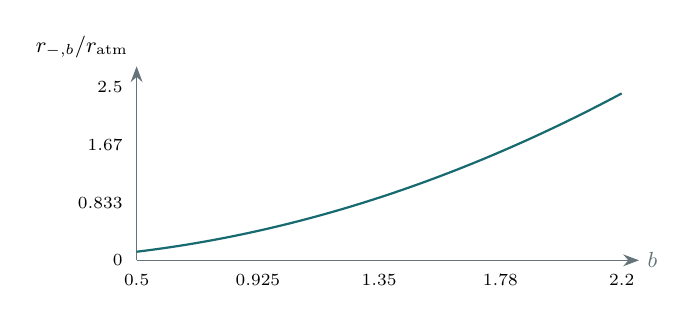
\begin{tikzpicture}[scale=.88,transform shape]
\draw[axis] (0,0.0000000)--(7.25,0.0000000) node[right] {$b$};
\draw[axis] (0.0000000,0)--(0.0000000,2.8);
\node[above left] at (0.0000000,2.8) {$r_{-,b}/r_{\rm atm}$};
\node[below,font=\scriptsize] at (0.0000000,-0.0800000) {$0.5$};
\node[below,font=\scriptsize] at (1.7500000,-0.0800000) {$0.925$};
\node[below,font=\scriptsize] at (3.5000000,-0.0800000) {$1.35$};
\node[below,font=\scriptsize] at (5.2500000,-0.0800000) {$1.78$};
\node[below,font=\scriptsize] at (7.0000000,-0.0800000) {$2.2$};
\node[left,font=\scriptsize] at (-0.0800000,0.0000000) {$0$};
\node[left,font=\scriptsize] at (-0.0800000,0.8333333) {$0.833$};
\node[left,font=\scriptsize] at (-0.0800000,1.6666667) {$1.67$};
\node[left,font=\scriptsize] at (-0.0800000,2.5000000) {$2.5$};
\draw[thick,color=accent] plot coordinates {(0.0000000,0.1239957) (0.0291667,0.1275345) (0.0583333,0.1311231) (0.0875000,0.1347615) (0.1166667,0.1384497) (0.1458333,0.1421878) (0.1750000,0.1459756) (0.2041667,0.1498133) (0.2333333,0.1537009) (0.2625000,0.1576382) (0.2916667,0.1616254) (0.3208333,0.1656624) (0.3500000,0.1697493) (0.3791667,0.1738860) (0.4083333,0.1780725) (0.4375000,0.1823089) (0.4666667,0.1865951) (0.4958333,0.1909311) (0.5250000,0.1953170) (0.5541667,0.1997528) (0.5833333,0.2042384) (0.6125000,0.2087738) (0.6416667,0.2133591) (0.6708333,0.2179943) (0.7000000,0.2226793) (0.7291667,0.2274141) (0.7583333,0.2321989) (0.7875000,0.2370335) (0.8166667,0.2419180) (0.8458333,0.2468523) (0.8750000,0.2518365) (0.9041667,0.2568706) (0.9333333,0.2619545) (0.9625000,0.2670884) (0.9916667,0.2722721) (1.0208333,0.2775057) (1.0500000,0.2827891) (1.0791667,0.2881225) (1.1083333,0.2935058) (1.1375000,0.2989389) (1.1666667,0.3044219) (1.1958333,0.3099549) (1.2250000,0.3155377) (1.2541667,0.3211704) (1.2833333,0.3268531) (1.3125000,0.3325856) (1.3416667,0.3383681) (1.3708333,0.3442004) (1.4000000,0.3500827) (1.4291667,0.3560149) (1.4583333,0.3619970) (1.4875000,0.3680290) (1.5166667,0.3741110) (1.5458333,0.3802429) (1.5750000,0.3864247) (1.6041667,0.3926564) (1.6333333,0.3989381) (1.6625000,0.4052697) (1.6916667,0.4116513) (1.7208333,0.4180828) (1.7500000,0.4245642) (1.7791667,0.4310956) (1.8083333,0.4376770) (1.8375000,0.4443083) (1.8666667,0.4509896) (1.8958333,0.4577208) (1.9250000,0.4645020) (1.9541667,0.4713331) (1.9833333,0.4782143) (2.0125000,0.4851454) (2.0416667,0.4921264) (2.0708333,0.4991575) (2.1000000,0.5062385) (2.1291667,0.5133695) (2.1583333,0.5205506) (2.1875000,0.5277816) (2.2166667,0.5350626) (2.2458333,0.5423936) (2.2750000,0.5497746) (2.3041667,0.5572056) (2.3333333,0.5646866) (2.3625000,0.5722176) (2.3916667,0.5797986) (2.4208333,0.5874297) (2.4500000,0.5951108) (2.4791667,0.6028419) (2.5083333,0.6106230) (2.5375000,0.6184542) (2.5666667,0.6263354) (2.5958333,0.6342666) (2.6250000,0.6422479) (2.6541667,0.6502792) (2.6833333,0.6583606) (2.7125000,0.6664921) (2.7416667,0.6746735) (2.7708333,0.6829051) (2.8000000,0.6911867) (2.8291667,0.6995184) (2.8583333,0.7079001) (2.8875000,0.7163320) (2.9166667,0.7248139) (2.9458333,0.7333459) (2.9750000,0.7419279) (3.0041667,0.7505601) (3.0333333,0.7592424) (3.0625000,0.7679747) (3.0916667,0.7767572) (3.1208333,0.7855898) (3.1500000,0.7944724) (3.1791667,0.8034052) (3.2083333,0.8123881) (3.2375000,0.8214212) (3.2666667,0.8305043) (3.2958333,0.8396376) (3.3250000,0.8488210) (3.3541667,0.8580546) (3.3833333,0.8673383) (3.4125000,0.8766721) (3.4416667,0.8860561) (3.4708333,0.8954903) (3.5000000,0.9049746) (3.5291667,0.9145091) (3.5583333,0.9240937) (3.5875000,0.9337285) (3.6166667,0.9434135) (3.6458333,0.9531487) (3.6750000,0.9629341) (3.7041667,0.9727696) (3.7333333,0.9826553) (3.7625000,0.9925913) (3.7916667,1.0025774) (3.8208333,1.0126138) (3.8500000,1.0227003) (3.8791667,1.0328371) (3.9083333,1.0430241) (3.9375000,1.0532613) (3.9666667,1.0635488) (3.9958333,1.0738864) (4.0250000,1.0842744) (4.0541667,1.0947125) (4.0833333,1.1052009) (4.1125000,1.1157396) (4.1416667,1.1263285) (4.1708333,1.1369677) (4.2000000,1.1476572) (4.2291667,1.1583969) (4.2583333,1.1691869) (4.2875000,1.1800272) (4.3166667,1.1909177) (4.3458333,1.2018586) (4.3750000,1.2128497) (4.4041667,1.2238912) (4.4333333,1.2349829) (4.4625000,1.2461250) (4.4916667,1.2573174) (4.5208333,1.2685601) (4.5500000,1.2798531) (4.5791667,1.2911965) (4.6083333,1.3025902) (4.6375000,1.3140343) (4.6666667,1.3255286) (4.6958333,1.3370734) (4.7250000,1.3486685) (4.7541667,1.3603139) (4.7833333,1.3720098) (4.8125000,1.3837560) (4.8416667,1.3955525) (4.8708333,1.4073995) (4.9000000,1.4192968) (4.9291667,1.4312446) (4.9583333,1.4432427) (4.9875000,1.4552913) (5.0166667,1.4673902) (5.0458333,1.4795396) (5.0750000,1.4917394) (5.1041667,1.5039896) (5.1333333,1.5162902) (5.1625000,1.5286413) (5.1916667,1.5410428) (5.2208333,1.5534948) (5.2500000,1.5659972) (5.2791667,1.5785501) (5.3083333,1.5911535) (5.3375000,1.6038073) (5.3666667,1.6165116) (5.3958333,1.6292664) (5.4250000,1.6420716) (5.4541667,1.6549274) (5.4833333,1.6678337) (5.5125000,1.6807904) (5.5416667,1.6937977) (5.5708333,1.7068555) (5.6000000,1.7199638) (5.6291667,1.7331227) (5.6583333,1.7463320) (5.6875000,1.7595920) (5.7166667,1.7729024) (5.7458333,1.7862635) (5.7750000,1.7996750) (5.8041667,1.8131372) (5.8333333,1.8266499) (5.8625000,1.8402132) (5.8916667,1.8538271) (5.9208333,1.8674915) (5.9500000,1.8812066) (5.9791667,1.8949722) (6.0083333,1.9087885) (6.0375000,1.9226554) (6.0666667,1.9365729) (6.0958333,1.9505410) (6.1250000,1.9645598) (6.1541667,1.9786292) (6.1833333,1.9927492) (6.2125000,2.0069199) (6.2416667,2.0211413) (6.2708333,2.0354133) (6.3000000,2.0497360) (6.3291667,2.0641094) (6.3583333,2.0785334) (6.3875000,2.0930082) (6.4166667,2.1075336) (6.4458333,2.1221098) (6.4750000,2.1367366) (6.5041667,2.1514142) (6.5333333,2.1661425) (6.5625000,2.1809215) (6.5916667,2.1957513) (6.6208333,2.2106318) (6.6500000,2.2255631) (6.6791667,2.2405451) (6.7083333,2.2555779) (6.7375000,2.2706614) (6.7666667,2.2857958) (6.7958333,2.3009809) (6.8250000,2.3162168) (6.8541667,2.3315035) (6.8833333,2.3468410) (6.9125000,2.3622293) (6.9416667,2.3776685) (6.9708333,2.3931584) (7.0000000,2.4086992)};
\end{tikzpicture}
\figcaption{变图综一.2V4\quad 短轴增大使形式近点移到入口圆外}
\end{minipage}\end{center}
变图综一.2V4画$r_{-,b}/r_{\rm atm}$。对极扁轨道，近点约按$b^2$增加，速度约按$1/b$降低；$b=2$时近点约$1.41\times10^5\ \mathrm{km}$，大于入口圆半径$7.1\times10^4\ \mathrm{km}$，整个椭圆留在入口圆外侧。临界短半轴由$B_{\rm crit}^2=2Ar_{\rm atm}-r_{\rm atm}^2$确定，约为$1.84\times10^6\ \mathrm{km}$。
\item \textbf{椭圆任一点的曲率。} 以参数角$\phi$表示轨道，求曲率半径并找出最大、最小值。
\par 从$x=A\cos\phi,y=B\sin\phi$求一、二阶导数，代入平面曲线曲率，得到
\[
\rho(\phi)=\frac{(A^2\sin^2\phi+B^2\cos^2\phi)^{3/2}}{AB}.
\]
\begin{center}\begin{minipage}{.98\linewidth}\centering
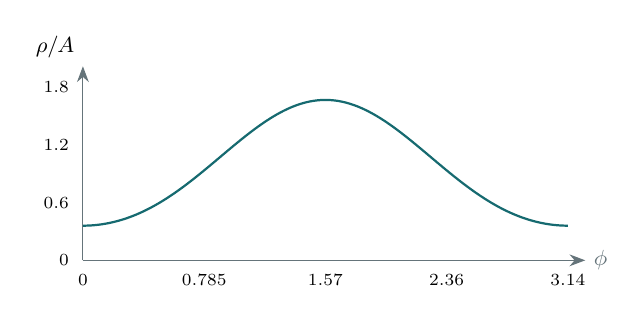
\begin{tikzpicture}[scale=.88,transform shape]
\draw[axis] (0,0.0000000)--(7.25,0.0000000) node[right] {$\phi$};
\draw[axis] (0.0000000,0)--(0.0000000,2.8);
\node[above left] at (0.0000000,2.8) {$\rho/A$};
\node[below,font=\scriptsize] at (0.0000000,-0.0800000) {$0$};
\node[below,font=\scriptsize] at (1.7500000,-0.0800000) {$0.785$};
\node[below,font=\scriptsize] at (3.5000000,-0.0800000) {$1.57$};
\node[below,font=\scriptsize] at (5.2500000,-0.0800000) {$2.36$};
\node[below,font=\scriptsize] at (7.0000000,-0.0800000) {$3.14$};
\node[left,font=\scriptsize] at (-0.0800000,0.0000000) {$0$};
\node[left,font=\scriptsize] at (-0.0800000,0.8333333) {$0.6$};
\node[left,font=\scriptsize] at (-0.0800000,1.6666667) {$1.2$};
\node[left,font=\scriptsize] at (-0.0800000,2.5000000) {$1.8$};
\draw[thick,color=accent] plot coordinates {(0.0000000,0.5000000) (0.0291667,0.5002285) (0.0583333,0.5009139) (0.0875000,0.5020565) (0.1166667,0.5036565) (0.1458333,0.5057143) (0.1750000,0.5082302) (0.2041667,0.5112048) (0.2333333,0.5146388) (0.2625000,0.5185327) (0.2916667,0.5228873) (0.3208333,0.5277032) (0.3500000,0.5329813) (0.3791667,0.5387223) (0.4083333,0.5449270) (0.4375000,0.5515960) (0.4666667,0.5587299) (0.4958333,0.5663294) (0.5250000,0.5743948) (0.5541667,0.5829266) (0.5833333,0.5919250) (0.6125000,0.6013899) (0.6416667,0.6113213) (0.6708333,0.6217188) (0.7000000,0.6325817) (0.7291667,0.6439093) (0.7583333,0.6557005) (0.7875000,0.6679538) (0.8166667,0.6806675) (0.8458333,0.6938395) (0.8750000,0.7074675) (0.9041667,0.7215486) (0.9333333,0.7360797) (0.9625000,0.7510571) (0.9916667,0.7664769) (1.0208333,0.7823346) (1.0500000,0.7986252) (1.0791667,0.8153435) (1.1083333,0.8324836) (1.1375000,0.8500390) (1.1666667,0.8680031) (1.1958333,0.8863684) (1.2250000,0.9051272) (1.2541667,0.9242710) (1.2833333,0.9437910) (1.3125000,0.9636777) (1.3416667,0.9839213) (1.3708333,1.0045113) (1.4000000,1.0254368) (1.4291667,1.0466861) (1.4583333,1.0682474) (1.4875000,1.0901081) (1.5166667,1.1122551) (1.5458333,1.1346749) (1.5750000,1.1573535) (1.6041667,1.1802764) (1.6333333,1.2034286) (1.6625000,1.2267946) (1.6916667,1.2503586) (1.7208333,1.2741042) (1.7500000,1.2980147) (1.7791667,1.3220730) (1.8083333,1.3462614) (1.8375000,1.3705621) (1.8666667,1.3949568) (1.8958333,1.4194269) (1.9250000,1.4439535) (1.9541667,1.4685175) (1.9833333,1.4930992) (2.0125000,1.5176791) (2.0416667,1.5422371) (2.0708333,1.5667531) (2.1000000,1.5912068) (2.1291667,1.6155777) (2.1583333,1.6398451) (2.1875000,1.6639884) (2.2166667,1.6879867) (2.2458333,1.7118191) (2.2750000,1.7354649) (2.3041667,1.7589031) (2.3333333,1.7821128) (2.3625000,1.8050732) (2.3916667,1.8277637) (2.4208333,1.8501635) (2.4500000,1.8722522) (2.4791667,1.8940094) (2.5083333,1.9154151) (2.5375000,1.9364492) (2.5666667,1.9570921) (2.5958333,1.9773244) (2.6250000,1.9971269) (2.6541667,2.0164807) (2.6833333,2.0353675) (2.7125000,2.0537691) (2.7416667,2.0716677) (2.7708333,2.0890461) (2.8000000,2.1058875) (2.8291667,2.1221753) (2.8583333,2.1378937) (2.8875000,2.1530273) (2.9166667,2.1675612) (2.9458333,2.1814811) (2.9750000,2.1947731) (3.0041667,2.2074242) (3.0333333,2.2194217) (3.0625000,2.2307537) (3.0916667,2.2414088) (3.1208333,2.2513765) (3.1500000,2.2606467) (3.1791667,2.2692100) (3.2083333,2.2770580) (3.2375000,2.2841827) (3.2666667,2.2905769) (3.2958333,2.2962341) (3.3250000,2.3011487) (3.3541667,2.3053156) (3.3833333,2.3087307) (3.4125000,2.3113905) (3.4416667,2.3132922) (3.4708333,2.3144341) (3.5000000,2.3148148) (3.5291667,2.3144341) (3.5583333,2.3132922) (3.5875000,2.3113905) (3.6166667,2.3087307) (3.6458333,2.3053156) (3.6750000,2.3011487) (3.7041667,2.2962341) (3.7333333,2.2905769) (3.7625000,2.2841827) (3.7916667,2.2770580) (3.8208333,2.2692100) (3.8500000,2.2606467) (3.8791667,2.2513765) (3.9083333,2.2414088) (3.9375000,2.2307537) (3.9666667,2.2194217) (3.9958333,2.2074242) (4.0250000,2.1947731) (4.0541667,2.1814811) (4.0833333,2.1675612) (4.1125000,2.1530273) (4.1416667,2.1378937) (4.1708333,2.1221753) (4.2000000,2.1058875) (4.2291667,2.0890461) (4.2583333,2.0716677) (4.2875000,2.0537691) (4.3166667,2.0353675) (4.3458333,2.0164807) (4.3750000,1.9971269) (4.4041667,1.9773244) (4.4333333,1.9570921) (4.4625000,1.9364492) (4.4916667,1.9154151) (4.5208333,1.8940094) (4.5500000,1.8722522) (4.5791667,1.8501635) (4.6083333,1.8277637) (4.6375000,1.8050732) (4.6666667,1.7821128) (4.6958333,1.7589031) (4.7250000,1.7354649) (4.7541667,1.7118191) (4.7833333,1.6879867) (4.8125000,1.6639884) (4.8416667,1.6398451) (4.8708333,1.6155777) (4.9000000,1.5912068) (4.9291667,1.5667531) (4.9583333,1.5422371) (4.9875000,1.5176791) (5.0166667,1.4930992) (5.0458333,1.4685175) (5.0750000,1.4439535) (5.1041667,1.4194269) (5.1333333,1.3949568) (5.1625000,1.3705621) (5.1916667,1.3462614) (5.2208333,1.3220730) (5.2500000,1.2980147) (5.2791667,1.2741042) (5.3083333,1.2503586) (5.3375000,1.2267946) (5.3666667,1.2034286) (5.3958333,1.1802764) (5.4250000,1.1573535) (5.4541667,1.1346749) (5.4833333,1.1122551) (5.5125000,1.0901081) (5.5416667,1.0682474) (5.5708333,1.0466861) (5.6000000,1.0254368) (5.6291667,1.0045113) (5.6583333,0.9839213) (5.6875000,0.9636777) (5.7166667,0.9437910) (5.7458333,0.9242710) (5.7750000,0.9051272) (5.8041667,0.8863684) (5.8333333,0.8680031) (5.8625000,0.8500390) (5.8916667,0.8324836) (5.9208333,0.8153435) (5.9500000,0.7986252) (5.9791667,0.7823346) (6.0083333,0.7664769) (6.0375000,0.7510571) (6.0666667,0.7360797) (6.0958333,0.7215486) (6.1250000,0.7074675) (6.1541667,0.6938395) (6.1833333,0.6806675) (6.2125000,0.6679538) (6.2416667,0.6557005) (6.2708333,0.6439093) (6.3000000,0.6325817) (6.3291667,0.6217188) (6.3583333,0.6113213) (6.3875000,0.6013899) (6.4166667,0.5919250) (6.4458333,0.5829266) (6.4750000,0.5743948) (6.5041667,0.5663294) (6.5333333,0.5587299) (6.5625000,0.5515960) (6.5916667,0.5449270) (6.6208333,0.5387223) (6.6500000,0.5329813) (6.6791667,0.5277032) (6.7083333,0.5228873) (6.7375000,0.5185327) (6.7666667,0.5146388) (6.7958333,0.5112048) (6.8250000,0.5082302) (6.8541667,0.5057143) (6.8833333,0.5036565) (6.9125000,0.5020565) (6.9416667,0.5009139) (6.9708333,0.5002285) (7.0000000,0.5000000)};
\end{tikzpicture}
\figcaption{变图综一.2V5\quad 长轴端曲率半径最小，短轴端最大}
\end{minipage}\end{center}
变图综一.2V5取$B/A=0.6$。括号随$\sin^2\phi$单调增大，故长轴两端$\rho_{\min}=B^2/A=0.36A$，短轴两端$\rho_{\max}=A^2/B=(5/3)A$。曲率半径描述轨道弯曲，和从力心到运动点的距离分别进入法向加速度与引力公式。
\item \textbf{离心率与两端速度。} 固定半长轴$A$和$GM$，以离心率$e$表示近、远点速度及二者之比。
\par 由$r_\mp=A(1\mp e)$代入机械能式，得到
\[
v_-=\sqrt{\frac{GM}{A}}\sqrt{\frac{1+e}{1-e}},\qquad
v_+=\sqrt{\frac{GM}{A}}\sqrt{\frac{1-e}{1+e}},\qquad
\frac{v_-}{v_+}=\frac{1+e}{1-e}.
\]
\begin{center}\begin{minipage}{.98\linewidth}\centering
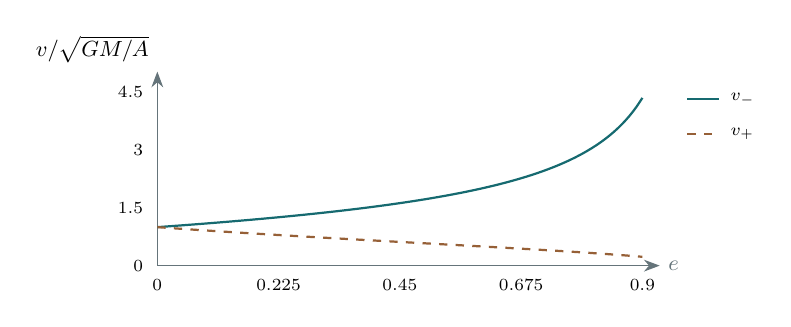
\begin{tikzpicture}[scale=.88,transform shape]
\draw[axis] (0,0.0000000)--(7.25,0.0000000) node[right] {$e$};
\draw[axis] (0.0000000,0)--(0.0000000,2.8);
\node[above left] at (0.0000000,2.8) {$v/\sqrt{GM/A}$};
\node[below,font=\scriptsize] at (0.0000000,-0.0800000) {$0$};
\node[below,font=\scriptsize] at (1.7500000,-0.0800000) {$0.225$};
\node[below,font=\scriptsize] at (3.5000000,-0.0800000) {$0.45$};
\node[below,font=\scriptsize] at (5.2500000,-0.0800000) {$0.675$};
\node[below,font=\scriptsize] at (7.0000000,-0.0800000) {$0.9$};
\node[left,font=\scriptsize] at (-0.0800000,0.0000000) {$0$};
\node[left,font=\scriptsize] at (-0.0800000,0.8333333) {$1.5$};
\node[left,font=\scriptsize] at (-0.0800000,1.6666667) {$3$};
\node[left,font=\scriptsize] at (-0.0800000,2.5000000) {$4.5$};
\draw[thick,color=accent] plot coordinates {(0.0000000,0.5555556) (0.0291667,0.5576428) (0.0583333,0.5597380) (0.0875000,0.5618411) (0.1166667,0.5639523) (0.1458333,0.5660717) (0.1750000,0.5681994) (0.2041667,0.5703354) (0.2333333,0.5724799) (0.2625000,0.5746329) (0.2916667,0.5767946) (0.3208333,0.5789650) (0.3500000,0.5811443) (0.3791667,0.5833325) (0.4083333,0.5855297) (0.4375000,0.5877361) (0.4666667,0.5899518) (0.4958333,0.5921768) (0.5250000,0.5944112) (0.5541667,0.5966553) (0.5833333,0.5989090) (0.6125000,0.6011726) (0.6416667,0.6034460) (0.6708333,0.6057295) (0.7000000,0.6080231) (0.7291667,0.6103269) (0.7583333,0.6126411) (0.7875000,0.6149659) (0.8166667,0.6173012) (0.8458333,0.6196473) (0.8750000,0.6220042) (0.9041667,0.6243721) (0.9333333,0.6267512) (0.9625000,0.6291415) (0.9916667,0.6315432) (1.0208333,0.6339564) (1.0500000,0.6363812) (1.0791667,0.6388179) (1.1083333,0.6412665) (1.1375000,0.6437271) (1.1666667,0.6462000) (1.1958333,0.6486852) (1.2250000,0.6511830) (1.2541667,0.6536934) (1.2833333,0.6562166) (1.3125000,0.6587528) (1.3416667,0.6613021) (1.3708333,0.6638647) (1.4000000,0.6664408) (1.4291667,0.6690305) (1.4583333,0.6716339) (1.4875000,0.6742513) (1.5166667,0.6768828) (1.5458333,0.6795287) (1.5750000,0.6821890) (1.6041667,0.6848639) (1.6333333,0.6875537) (1.6625000,0.6902585) (1.6916667,0.6929786) (1.7208333,0.6957140) (1.7500000,0.6984651) (1.7791667,0.7012319) (1.8083333,0.7040148) (1.8375000,0.7068138) (1.8666667,0.7096293) (1.8958333,0.7124614) (1.9250000,0.7153104) (1.9541667,0.7181764) (1.9833333,0.7210597) (2.0125000,0.7239605) (2.0416667,0.7268791) (2.0708333,0.7298156) (2.1000000,0.7327704) (2.1291667,0.7357436) (2.1583333,0.7387356) (2.1875000,0.7417465) (2.2166667,0.7447766) (2.2458333,0.7478262) (2.2750000,0.7508956) (2.3041667,0.7539849) (2.3333333,0.7570946) (2.3625000,0.7602248) (2.3916667,0.7633759) (2.4208333,0.7665481) (2.4500000,0.7697418) (2.4791667,0.7729572) (2.5083333,0.7761947) (2.5375000,0.7794546) (2.5666667,0.7827371) (2.5958333,0.7860426) (2.6250000,0.7893715) (2.6541667,0.7927241) (2.6833333,0.7961007) (2.7125000,0.7995016) (2.7416667,0.8029273) (2.7708333,0.8063781) (2.8000000,0.8098544) (2.8291667,0.8133566) (2.8583333,0.8168850) (2.8875000,0.8204400) (2.9166667,0.8240221) (2.9458333,0.8276316) (2.9750000,0.8312690) (3.0041667,0.8349347) (3.0333333,0.8386292) (3.0625000,0.8423529) (3.0916667,0.8461062) (3.1208333,0.8498897) (3.1500000,0.8537037) (3.1791667,0.8575489) (3.2083333,0.8614256) (3.2375000,0.8653345) (3.2666667,0.8692760) (3.2958333,0.8732506) (3.3250000,0.8772590) (3.3541667,0.8813016) (3.3833333,0.8853790) (3.4125000,0.8894919) (3.4416667,0.8936408) (3.4708333,0.8978263) (3.5000000,0.9020490) (3.5291667,0.9063097) (3.5583333,0.9106089) (3.5875000,0.9149474) (3.6166667,0.9193257) (3.6458333,0.9237447) (3.6750000,0.9282050) (3.7041667,0.9327074) (3.7333333,0.9372527) (3.7625000,0.9418415) (3.7916667,0.9464748) (3.8208333,0.9511533) (3.8500000,0.9558779) (3.8791667,0.9606494) (3.9083333,0.9654687) (3.9375000,0.9703367) (3.9666667,0.9752544) (3.9958333,0.9802227) (4.0250000,0.9852426) (4.0541667,0.9903151) (4.0833333,0.9954412) (4.1125000,1.0006220) (4.1416667,1.0058586) (4.1708333,1.0111521) (4.2000000,1.0165036) (4.2291667,1.0219145) (4.2583333,1.0273857) (4.2875000,1.0329188) (4.3166667,1.0385148) (4.3458333,1.0441752) (4.3750000,1.0499013) (4.4041667,1.0556946) (4.4333333,1.0615564) (4.4625000,1.0674884) (4.4916667,1.0734920) (4.5208333,1.0795689) (4.5500000,1.0857206) (4.5791667,1.0919489) (4.6083333,1.0982556) (4.6375000,1.1046423) (4.6666667,1.1111111) (4.6958333,1.1176638) (4.7250000,1.1243024) (4.7541667,1.1310290) (4.7833333,1.1378458) (4.8125000,1.1447548) (4.8416667,1.1517584) (4.8708333,1.1588589) (4.9000000,1.1660588) (4.9291667,1.1733605) (4.9583333,1.1807668) (4.9875000,1.1882803) (5.0166667,1.1959039) (5.0458333,1.2036403) (5.0750000,1.2114928) (5.1041667,1.2194643) (5.1333333,1.2275582) (5.1625000,1.2357778) (5.1916667,1.2441266) (5.2208333,1.2526084) (5.2500000,1.2612269) (5.2791667,1.2699860) (5.3083333,1.2788899) (5.3375000,1.2879429) (5.3666667,1.2971494) (5.3958333,1.3065141) (5.4250000,1.3160418) (5.4541667,1.3257377) (5.4833333,1.3356070) (5.5125000,1.3456552) (5.5416667,1.3558881) (5.5708333,1.3663118) (5.6000000,1.3769327) (5.6291667,1.3877572) (5.6583333,1.3987924) (5.6875000,1.4100456) (5.7166667,1.4215243) (5.7458333,1.4332367) (5.7750000,1.4451911) (5.8041667,1.4573964) (5.8333333,1.4698618) (5.8625000,1.4825973) (5.8916667,1.4956132) (5.9208333,1.5089203) (5.9500000,1.5225302) (5.9791667,1.5364550) (6.0083333,1.5507076) (6.0375000,1.5653016) (6.0666667,1.5802513) (6.0958333,1.5955721) (6.1250000,1.6112801) (6.1541667,1.6273927) (6.1833333,1.6439280) (6.2125000,1.6609056) (6.2416667,1.6783463) (6.2708333,1.6962723) (6.3000000,1.7147072) (6.3291667,1.7336765) (6.3583333,1.7532073) (6.3875000,1.7733287) (6.4166667,1.7940722) (6.4458333,1.8154712) (6.4750000,1.8375623) (6.5041667,1.8603846) (6.5333333,1.8839806) (6.5625000,1.9083960) (6.5916667,1.9336809) (6.6208333,1.9598893) (6.6500000,1.9870805) (6.6791667,2.0153188) (6.7083333,2.0446750) (6.7375000,2.0752265) (6.7666667,2.1070586) (6.7958333,2.1402654) (6.8250000,2.1749507) (6.8541667,2.2112301) (6.8833333,2.2492320) (6.9125000,2.2890998) (6.9416667,2.3309943) (6.9708333,2.3750964) (7.0000000,2.4216105)};
\draw[thick,color=accent] (7.65,2.4)--(8.1,2.4);\node[right,font=\scriptsize] at (8.15,2.4) {$v_-$};
\draw[thick,dashed,color=warm] plot coordinates {(0.0000000,0.5555556) (0.0291667,0.5534761) (0.0583333,0.5514044) (0.0875000,0.5493403) (0.1166667,0.5472838) (0.1458333,0.5452347) (0.1750000,0.5431931) (0.2041667,0.5411587) (0.2333333,0.5391316) (0.2625000,0.5371115) (0.2916667,0.5350986) (0.3208333,0.5330926) (0.3500000,0.5310936) (0.3791667,0.5291013) (0.4083333,0.5271158) (0.4375000,0.5251370) (0.4666667,0.5231648) (0.4958333,0.5211991) (0.5250000,0.5192398) (0.5541667,0.5172869) (0.5833333,0.5153403) (0.6125000,0.5134000) (0.6416667,0.5114658) (0.6708333,0.5095377) (0.7000000,0.5076156) (0.7291667,0.5056994) (0.7583333,0.5037892) (0.7875000,0.5018847) (0.8166667,0.4999860) (0.8458333,0.4980930) (0.8750000,0.4962056) (0.9041667,0.4943237) (0.9333333,0.4924474) (0.9625000,0.4905764) (0.9916667,0.4887108) (1.0208333,0.4868505) (1.0500000,0.4849954) (1.0791667,0.4831455) (1.1083333,0.4813007) (1.1375000,0.4794609) (1.1666667,0.4776261) (1.1958333,0.4757962) (1.2250000,0.4739712) (1.2541667,0.4721510) (1.2833333,0.4703355) (1.3125000,0.4685247) (1.3416667,0.4667186) (1.3708333,0.4649170) (1.4000000,0.4631199) (1.4291667,0.4613272) (1.4583333,0.4595390) (1.4875000,0.4577551) (1.5166667,0.4559755) (1.5458333,0.4542001) (1.5750000,0.4524289) (1.6041667,0.4506618) (1.6333333,0.4488987) (1.6625000,0.4471397) (1.6916667,0.4453846) (1.7208333,0.4436334) (1.7500000,0.4418861) (1.7791667,0.4401425) (1.8083333,0.4384027) (1.8375000,0.4366666) (1.8666667,0.4349341) (1.8958333,0.4332052) (1.9250000,0.4314798) (1.9541667,0.4297579) (1.9833333,0.4280394) (2.0125000,0.4263243) (2.0416667,0.4246125) (2.0708333,0.4229040) (2.1000000,0.4211987) (2.1291667,0.4194966) (2.1583333,0.4177976) (2.1875000,0.4161017) (2.2166667,0.4144088) (2.2458333,0.4127188) (2.2750000,0.4110318) (2.3041667,0.4093477) (2.3333333,0.4076663) (2.3625000,0.4059878) (2.3916667,0.4043119) (2.4208333,0.4026387) (2.4500000,0.4009682) (2.4791667,0.3993002) (2.5083333,0.3976347) (2.5375000,0.3959717) (2.5666667,0.3943112) (2.5958333,0.3926530) (2.6250000,0.3909971) (2.6541667,0.3893435) (2.6833333,0.3876921) (2.7125000,0.3860430) (2.7416667,0.3843959) (2.7708333,0.3827509) (2.8000000,0.3811080) (2.8291667,0.3794670) (2.8583333,0.3778280) (2.8875000,0.3761908) (2.9166667,0.3745555) (2.9458333,0.3729219) (2.9750000,0.3712901) (3.0041667,0.3696600) (3.0333333,0.3680315) (3.0625000,0.3664046) (3.0916667,0.3647792) (3.1208333,0.3631553) (3.1500000,0.3615329) (3.1791667,0.3599118) (3.2083333,0.3582921) (3.2375000,0.3566736) (3.2666667,0.3550564) (3.2958333,0.3534403) (3.3250000,0.3518254) (3.3541667,0.3502115) (3.3833333,0.3485987) (3.4125000,0.3469868) (3.4416667,0.3453759) (3.4708333,0.3437658) (3.5000000,0.3421565) (3.5291667,0.3405480) (3.5583333,0.3389402) (3.5875000,0.3373330) (3.6166667,0.3357265) (3.6458333,0.3341204) (3.6750000,0.3325149) (3.7041667,0.3309097) (3.7333333,0.3293050) (3.7625000,0.3277005) (3.7916667,0.3260964) (3.8208333,0.3244924) (3.8500000,0.3228885) (3.8791667,0.3212847) (3.9083333,0.3196810) (3.9375000,0.3180772) (3.9666667,0.3164733) (3.9958333,0.3148692) (4.0250000,0.3132649) (4.0541667,0.3116604) (4.0833333,0.3100555) (4.1125000,0.3084501) (4.1416667,0.3068443) (4.1708333,0.3052379) (4.2000000,0.3036310) (4.2291667,0.3020233) (4.2583333,0.3004149) (4.2875000,0.2988057) (4.3166667,0.2971956) (4.3458333,0.2955845) (4.3750000,0.2939724) (4.4041667,0.2923592) (4.4333333,0.2907448) (4.4625000,0.2891291) (4.4916667,0.2875121) (4.5208333,0.2858937) (4.5500000,0.2842738) (4.5791667,0.2826524) (4.6083333,0.2810293) (4.6375000,0.2794044) (4.6666667,0.2777778) (4.6958333,0.2761492) (4.7250000,0.2745186) (4.7541667,0.2728860) (4.7833333,0.2712512) (4.8125000,0.2696141) (4.8416667,0.2679746) (4.8708333,0.2663327) (4.9000000,0.2646882) (4.9291667,0.2630410) (4.9583333,0.2613911) (4.9875000,0.2597384) (5.0166667,0.2580826) (5.0458333,0.2564238) (5.0750000,0.2547617) (5.1041667,0.2530964) (5.1333333,0.2514276) (5.1625000,0.2497552) (5.1916667,0.2480792) (5.2208333,0.2463994) (5.2500000,0.2447157) (5.2791667,0.2430279) (5.3083333,0.2413358) (5.3375000,0.2396395) (5.3666667,0.2379386) (5.3958333,0.2362332) (5.4250000,0.2345229) (5.4541667,0.2328077) (5.4833333,0.2310874) (5.5125000,0.2293619) (5.5416667,0.2276309) (5.5708333,0.2258942) (5.6000000,0.2241518) (5.6291667,0.2224034) (5.6583333,0.2206489) (5.6875000,0.2188879) (5.7166667,0.2171204) (5.7458333,0.2153461) (5.7750000,0.2135648) (5.8041667,0.2117763) (5.8333333,0.2099803) (5.8625000,0.2081765) (5.8916667,0.2063648) (5.9208333,0.2045449) (5.9500000,0.2027165) (5.9791667,0.2008793) (6.0083333,0.1990330) (6.0375000,0.1971773) (6.0666667,0.1953120) (6.0958333,0.1934366) (6.1250000,0.1915508) (6.1541667,0.1896543) (6.1833333,0.1877467) (6.2125000,0.1858275) (6.2416667,0.1838965) (6.2708333,0.1819531) (6.3000000,0.1799969) (6.3291667,0.1780274) (6.3583333,0.1760442) (6.3875000,0.1740467) (6.4166667,0.1720343) (6.4458333,0.1700065) (6.4750000,0.1679627) (6.5041667,0.1659022) (6.5333333,0.1638244) (6.5625000,0.1617285) (6.5916667,0.1596137) (6.6208333,0.1574793) (6.6500000,0.1553243) (6.6791667,0.1531480) (6.7083333,0.1509492) (6.7375000,0.1487269) (6.7666667,0.1464800) (6.7958333,0.1442073) (6.8250000,0.1419076) (6.8541667,0.1395793) (6.8833333,0.1372210) (6.9125000,0.1348312) (6.9416667,0.1324079) (6.9708333,0.1299492) (7.0000000,0.1274532)};
\draw[thick,dashed,color=warm] (7.65,1.9)--(8.1,1.9);\node[right,font=\scriptsize] at (8.15,1.9) {$v_+$};
\end{tikzpicture}
\figcaption{变图综一.2V6\quad 固定半长轴时两端速度随离心率分离}
\end{minipage}\end{center}
变图综一.2V6中$e=0$时两端速度都等于圆速度；$e$增大时近点速度升高、远点速度降低，而周期仍由$A$决定。两端速度的乘积为$GM/A$，与端点角动量关系同时成立。
\item \textbf{只改变半长轴。} 在相同引力参数下，将半长轴从$A_0$改为$\lambda A_0$，保持离心率相同，求周期、两端速度和角动量的尺度变化。
\par 由周期、端点速度和半通径公式分别得到
\[
\frac T{T_0}=\lambda^{3/2},\qquad
\frac{v_\mp}{v_{\mp0}}=\lambda^{-1/2},\qquad
\frac h{h_0}=\lambda^{1/2}.
\]
\begin{center}\begin{minipage}{.98\linewidth}\centering
\begin{tikzpicture}[scale=.88,transform shape]
\draw[axis] (0,0.0000000)--(7.25,0.0000000) node[right] {$\lambda=A/A_0$};
\draw[axis] (0.0000000,0)--(0.0000000,2.8);
\node[above left] at (0.0000000,2.8) {$T/T_0$};
\node[below,font=\scriptsize] at (0.0000000,-0.0800000) {$0.5$};
\node[below,font=\scriptsize] at (1.7500000,-0.0800000) {$0.875$};
\node[below,font=\scriptsize] at (3.5000000,-0.0800000) {$1.25$};
\node[below,font=\scriptsize] at (5.2500000,-0.0800000) {$1.62$};
\node[below,font=\scriptsize] at (7.0000000,-0.0800000) {$2$};
\node[left,font=\scriptsize] at (-0.0800000,0.0000000) {$0$};
\node[left,font=\scriptsize] at (-0.0800000,0.8333333) {$1$};
\node[left,font=\scriptsize] at (-0.0800000,1.6666667) {$2$};
\node[left,font=\scriptsize] at (-0.0800000,2.5000000) {$3$};
\draw[thick,color=accent] plot coordinates {(0.0000000,0.2946278) (0.0291667,0.3001693) (0.0583333,0.3057451) (0.0875000,0.3113551) (0.1166667,0.3169989) (0.1458333,0.3226764) (0.1750000,0.3283874) (0.2041667,0.3341317) (0.2333333,0.3399091) (0.2625000,0.3457194) (0.2916667,0.3515625) (0.3208333,0.3574381) (0.3500000,0.3633461) (0.3791667,0.3692863) (0.4083333,0.3752585) (0.4375000,0.3812626) (0.4666667,0.3872983) (0.4958333,0.3933656) (0.5250000,0.3994642) (0.5541667,0.4055940) (0.5833333,0.4117549) (0.6125000,0.4179466) (0.6416667,0.4241691) (0.6708333,0.4304222) (0.7000000,0.4367056) (0.7291667,0.4430194) (0.7583333,0.4493633) (0.7875000,0.4557372) (0.8166667,0.4621409) (0.8458333,0.4685744) (0.8750000,0.4750374) (0.9041667,0.4815299) (0.9333333,0.4880517) (0.9625000,0.4946027) (0.9916667,0.5011827) (1.0208333,0.5077916) (1.0500000,0.5144294) (1.0791667,0.5210958) (1.1083333,0.5277908) (1.1375000,0.5345142) (1.1666667,0.5412659) (1.1958333,0.5480458) (1.2250000,0.5548538) (1.2541667,0.5616897) (1.2833333,0.5685535) (1.3125000,0.5754450) (1.3416667,0.5823641) (1.3708333,0.5893107) (1.4000000,0.5962848) (1.4291667,0.6032861) (1.4583333,0.6103147) (1.4875000,0.6173703) (1.5166667,0.6244529) (1.5458333,0.6315624) (1.5750000,0.6386986) (1.6041667,0.6458616) (1.6333333,0.6530511) (1.6625000,0.6602671) (1.6916667,0.6675094) (1.7208333,0.6747781) (1.7500000,0.6820730) (1.7791667,0.6893939) (1.8083333,0.6967409) (1.8375000,0.7041138) (1.8666667,0.7115125) (1.8958333,0.7189369) (1.9250000,0.7263870) (1.9541667,0.7338626) (1.9833333,0.7413638) (2.0125000,0.7488903) (2.0416667,0.7564421) (2.0708333,0.7640191) (2.1000000,0.7716212) (2.1291667,0.7792484) (2.1583333,0.7869006) (2.1875000,0.7945776) (2.2166667,0.8022795) (2.2458333,0.8100060) (2.2750000,0.8177573) (2.3041667,0.8255331) (2.3333333,0.8333333) (2.3625000,0.8411580) (2.3916667,0.8490071) (2.4208333,0.8568804) (2.4500000,0.8647778) (2.4791667,0.8726994) (2.5083333,0.8806451) (2.5375000,0.8886147) (2.5666667,0.8966082) (2.5958333,0.9046255) (2.6250000,0.9126666) (2.6541667,0.9207314) (2.6833333,0.9288198) (2.7125000,0.9369317) (2.7416667,0.9450671) (2.7708333,0.9532259) (2.8000000,0.9614081) (2.8291667,0.9696136) (2.8583333,0.9778422) (2.8875000,0.9860940) (2.9166667,0.9943689) (2.9458333,1.0026668) (2.9750000,1.0109877) (3.0041667,1.0193314) (3.0333333,1.0276980) (3.0625000,1.0360874) (3.0916667,1.0444994) (3.1208333,1.0529341) (3.1500000,1.0613914) (3.1791667,1.0698712) (3.2083333,1.0783734) (3.2375000,1.0868981) (3.2666667,1.0954451) (3.2958333,1.1040144) (3.3250000,1.1126059) (3.3541667,1.1212196) (3.3833333,1.1298555) (3.4125000,1.1385133) (3.4416667,1.1471932) (3.4708333,1.1558950) (3.5000000,1.1646187) (3.5291667,1.1733643) (3.5583333,1.1821316) (3.5875000,1.1909207) (3.6166667,1.1997314) (3.6458333,1.2085638) (3.6750000,1.2174177) (3.7041667,1.2262931) (3.7333333,1.2351900) (3.7625000,1.2441084) (3.7916667,1.2530480) (3.8208333,1.2620090) (3.8500000,1.2709913) (3.8791667,1.2799947) (3.9083333,1.2890194) (3.9375000,1.2980651) (3.9666667,1.3071319) (3.9958333,1.3162197) (4.0250000,1.3253284) (4.0541667,1.3344581) (4.0833333,1.3436087) (4.1125000,1.3527801) (4.1416667,1.3619722) (4.1708333,1.3711851) (4.2000000,1.3804186) (4.2291667,1.3896728) (4.2583333,1.3989476) (4.2875000,1.4082429) (4.3166667,1.4175587) (4.3458333,1.4268950) (4.3750000,1.4362516) (4.4041667,1.4456287) (4.4333333,1.4550260) (4.4625000,1.4644436) (4.4916667,1.4738815) (4.5208333,1.4833395) (4.5500000,1.4928177) (4.5791667,1.5023160) (4.6083333,1.5118344) (4.6375000,1.5213727) (4.6666667,1.5309311) (4.6958333,1.5405094) (4.7250000,1.5501075) (4.7541667,1.5597256) (4.7833333,1.5693634) (4.8125000,1.5790210) (4.8416667,1.5886983) (4.8708333,1.5983954) (4.9000000,1.6081120) (4.9291667,1.6178483) (4.9583333,1.6276042) (4.9875000,1.6373796) (5.0166667,1.6471744) (5.0458333,1.6569888) (5.0750000,1.6668225) (5.1041667,1.6766756) (5.1333333,1.6865481) (5.1625000,1.6964398) (5.1916667,1.7063509) (5.2208333,1.7162811) (5.2500000,1.7262306) (5.2791667,1.7361992) (5.3083333,1.7461869) (5.3375000,1.7561937) (5.3666667,1.7662195) (5.3958333,1.7762643) (5.4250000,1.7863281) (5.4541667,1.7964109) (5.4833333,1.8065125) (5.5125000,1.8166330) (5.5416667,1.8267723) (5.5708333,1.8369305) (5.6000000,1.8471073) (5.6291667,1.8573030) (5.6583333,1.8675173) (5.6875000,1.8777502) (5.7166667,1.8880018) (5.7458333,1.8982720) (5.7750000,1.9085607) (5.8041667,1.9188679) (5.8333333,1.9291937) (5.8625000,1.9395379) (5.8916667,1.9499005) (5.9208333,1.9602815) (5.9500000,1.9706808) (5.9791667,1.9810985) (6.0083333,1.9915345) (6.0375000,2.0019887) (6.0666667,2.0124612) (6.0958333,2.0229518) (6.1250000,2.0334607) (6.1541667,2.0439876) (6.1833333,2.0545327) (6.2125000,2.0650958) (6.2416667,2.0756770) (6.2708333,2.0862762) (6.3000000,2.0968934) (6.3291667,2.1075285) (6.3583333,2.1181815) (6.3875000,2.1288525) (6.4166667,2.1395412) (6.4458333,2.1502479) (6.4750000,2.1609723) (6.5041667,2.1717145) (6.5333333,2.1824744) (6.5625000,2.1932520) (6.5916667,2.2040473) (6.6208333,2.2148603) (6.6500000,2.2256909) (6.6791667,2.2365391) (6.7083333,2.2474049) (6.7375000,2.2582882) (6.7666667,2.2691890) (6.7958333,2.2801073) (6.8250000,2.2910431) (6.8541667,2.3019962) (6.8833333,2.3129668) (6.9125000,2.3239548) (6.9416667,2.3349601) (6.9708333,2.3459827) (7.0000000,2.3570226)};
\end{tikzpicture}
\figcaption{变图综一.2V7\quad 周期随半长轴的二分之三次幂增加}
\end{minipage}\end{center}
变图综一.2V7画周期比。半长轴增倍时，周期增为$2\sqrt2$倍，近、远点速度各降为$1/\sqrt2$倍，单位质量角动量增为$\sqrt2$倍。这三种尺度分别反映轨道长度、引力强度和面积速度的变化。
\item \textbf{入口速度的方向。} 用题给轨道求入口处的径向与切向速度，并求速度相对于当地切线的夹角。
\par 半通径$p=B^2/A$，单位质量角动量$h=\sqrt{GMp}$。在入口$r=r_{\rm atm}$，有
\[
v_t=\frac h{r_{\rm atm}},\qquad
v_r=-\sqrt{GM\left(\frac2{r_{\rm atm}}-\frac1A\right)-\frac{h^2}{r_{\rm atm}^2}},\qquad
\tan\psi=\frac{|v_r|}{v_t}.
\]
\begin{center}\begin{minipage}{.98\linewidth}\centering
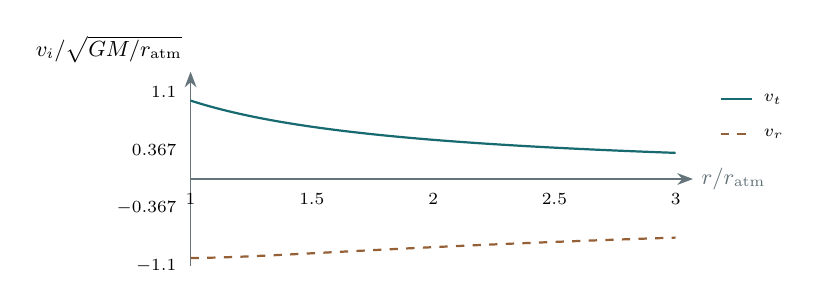
\begin{tikzpicture}[scale=.88,transform shape]
\draw[axis] (0,1.2500000)--(7.25,1.2500000) node[right] {$r/r_{\rm atm}$};
\draw[axis] (0.0000000,0)--(0.0000000,2.8);
\node[above left] at (0.0000000,2.8) {$v_i/\sqrt{GM/r_{\rm atm}}$};
\node[below,font=\scriptsize] at (0.0000000,1.1700000) {$1$};
\node[below,font=\scriptsize] at (1.7500000,1.1700000) {$1.5$};
\node[below,font=\scriptsize] at (3.5000000,1.1700000) {$2$};
\node[below,font=\scriptsize] at (5.2500000,1.1700000) {$2.5$};
\node[below,font=\scriptsize] at (7.0000000,1.1700000) {$3$};
\node[left,font=\scriptsize] at (-0.0800000,0.0000000) {$-1.1$};
\node[left,font=\scriptsize] at (-0.0800000,0.8333333) {$-0.367$};
\node[left,font=\scriptsize] at (-0.0800000,1.6666667) {$0.367$};
\node[left,font=\scriptsize] at (-0.0800000,2.5000000) {$1.1$};
\draw[thick,color=accent] plot coordinates {(0.0000000,2.3816858) (0.0291667,2.3723331) (0.0583333,2.3631336) (0.0875000,2.3540838) (0.1166667,2.3451799) (0.1458333,2.3364184) (0.1750000,2.3277960) (0.2041667,2.3193095) (0.2333333,2.3109555) (0.2625000,2.3027310) (0.2916667,2.2946331) (0.3208333,2.2866588) (0.3500000,2.2788053) (0.3791667,2.2710699) (0.4083333,2.2634500) (0.4375000,2.2559430) (0.4666667,2.2485463) (0.4958333,2.2412577) (0.5250000,2.2340747) (0.5541667,2.2269950) (0.5833333,2.2200164) (0.6125000,2.2131369) (0.6416667,2.2063542) (0.6708333,2.1996664) (0.7000000,2.1930715) (0.7291667,2.1865676) (0.7583333,2.1801528) (0.7875000,2.1738252) (0.8166667,2.1675831) (0.8458333,2.1614248) (0.8750000,2.1553487) (0.9041667,2.1493530) (0.9333333,2.1434362) (0.9625000,2.1375967) (0.9916667,2.1318331) (1.0208333,2.1261439) (1.0500000,2.1205276) (1.0791667,2.1149828) (1.1083333,2.1095082) (1.1375000,2.1041025) (1.1666667,2.0987644) (1.1958333,2.0934926) (1.2250000,2.0882858) (1.2541667,2.0831430) (1.2833333,2.0780628) (1.3125000,2.0730443) (1.3416667,2.0680862) (1.3708333,2.0631874) (1.4000000,2.0583470) (1.4291667,2.0535639) (1.4583333,2.0488371) (1.4875000,2.0441655) (1.5166667,2.0395483) (1.5458333,2.0349844) (1.5750000,2.0304730) (1.6041667,2.0260132) (1.6333333,2.0216040) (1.6625000,2.0172446) (1.6916667,2.0129343) (1.7208333,2.0086721) (1.7500000,2.0044572) (1.7791667,2.0002890) (1.8083333,1.9961665) (1.8375000,1.9920891) (1.8666667,1.9880560) (1.8958333,1.9840665) (1.9250000,1.9801199) (1.9541667,1.9762155) (1.9833333,1.9723527) (2.0125000,1.9685307) (2.0416667,1.9647490) (2.0708333,1.9610068) (2.1000000,1.9573037) (2.1291667,1.9536389) (2.1583333,1.9500119) (2.1875000,1.9464221) (2.2166667,1.9428689) (2.2458333,1.9393518) (2.2750000,1.9358702) (2.3041667,1.9324236) (2.3333333,1.9290115) (2.3625000,1.9256333) (2.3916667,1.9222886) (2.4208333,1.9189769) (2.4500000,1.9156976) (2.4791667,1.9124503) (2.5083333,1.9092345) (2.5375000,1.9060498) (2.5666667,1.9028957) (2.5958333,1.8997718) (2.6250000,1.8966776) (2.6541667,1.8936128) (2.6833333,1.8905769) (2.7125000,1.8875695) (2.7416667,1.8845902) (2.7708333,1.8816386) (2.8000000,1.8787144) (2.8291667,1.8758171) (2.8583333,1.8729463) (2.8875000,1.8701018) (2.9166667,1.8672832) (2.9458333,1.8644901) (2.9750000,1.8617221) (3.0041667,1.8589789) (3.0333333,1.8562603) (3.0625000,1.8535658) (3.0916667,1.8508951) (3.1208333,1.8482480) (3.1500000,1.8456241) (3.1791667,1.8430232) (3.2083333,1.8404448) (3.2375000,1.8378888) (3.2666667,1.8353547) (3.2958333,1.8328425) (3.3250000,1.8303517) (3.3541667,1.8278821) (3.3833333,1.8254335) (3.4125000,1.8230055) (3.4416667,1.8205979) (3.4708333,1.8182105) (3.5000000,1.8158429) (3.5291667,1.8134950) (3.5583333,1.8111665) (3.5875000,1.8088572) (3.6166667,1.8065668) (3.6458333,1.8042951) (3.6750000,1.8020419) (3.7041667,1.7998069) (3.7333333,1.7975899) (3.7625000,1.7953908) (3.7916667,1.7932092) (3.8208333,1.7910450) (3.8500000,1.7888980) (3.8791667,1.7867680) (3.9083333,1.7846547) (3.9375000,1.7825580) (3.9666667,1.7804777) (3.9958333,1.7784136) (4.0250000,1.7763655) (4.0541667,1.7743332) (4.0833333,1.7723165) (4.1125000,1.7703153) (4.1416667,1.7683294) (4.1708333,1.7663586) (4.2000000,1.7644027) (4.2291667,1.7624615) (4.2583333,1.7605350) (4.2875000,1.7586229) (4.3166667,1.7567250) (4.3458333,1.7548413) (4.3750000,1.7529715) (4.4041667,1.7511155) (4.4333333,1.7492732) (4.4625000,1.7474443) (4.4916667,1.7456288) (4.5208333,1.7438266) (4.5500000,1.7420373) (4.5791667,1.7402610) (4.6083333,1.7384975) (4.6375000,1.7367466) (4.6666667,1.7350082) (4.6958333,1.7332822) (4.7250000,1.7315684) (4.7541667,1.7298668) (4.7833333,1.7281771) (4.8125000,1.7264993) (4.8416667,1.7248332) (4.8708333,1.7231788) (4.9000000,1.7215358) (4.9291667,1.7199042) (4.9583333,1.7182838) (4.9875000,1.7166746) (5.0166667,1.7150764) (5.0458333,1.7134891) (5.0750000,1.7119126) (5.1041667,1.7103468) (5.1333333,1.7087916) (5.1625000,1.7072468) (5.1916667,1.7057124) (5.2208333,1.7041883) (5.2500000,1.7026743) (5.2791667,1.7011704) (5.3083333,1.6996765) (5.3375000,1.6981924) (5.3666667,1.6967181) (5.3958333,1.6952534) (5.4250000,1.6937984) (5.4541667,1.6923528) (5.4833333,1.6909166) (5.5125000,1.6894896) (5.5416667,1.6880719) (5.5708333,1.6866633) (5.6000000,1.6852638) (5.6291667,1.6838732) (5.6583333,1.6824914) (5.6875000,1.6811184) (5.7166667,1.6797541) (5.7458333,1.6783984) (5.7750000,1.6770513) (5.8041667,1.6757125) (5.8333333,1.6743822) (5.8625000,1.6730601) (5.8916667,1.6717463) (5.9208333,1.6704406) (5.9500000,1.6691429) (5.9791667,1.6678532) (6.0083333,1.6665715) (6.0375000,1.6652976) (6.0666667,1.6640314) (6.0958333,1.6627730) (6.1250000,1.6615221) (6.1541667,1.6602789) (6.1833333,1.6590431) (6.2125000,1.6578147) (6.2416667,1.6565937) (6.2708333,1.6553800) (6.3000000,1.6541735) (6.3291667,1.6529742) (6.3583333,1.6517820) (6.3875000,1.6505968) (6.4166667,1.6494185) (6.4458333,1.6482472) (6.4750000,1.6470828) (6.5041667,1.6459251) (6.5333333,1.6447741) (6.5625000,1.6436299) (6.5916667,1.6424922) (6.6208333,1.6413611) (6.6500000,1.6402365) (6.6791667,1.6391183) (6.7083333,1.6380066) (6.7375000,1.6369011) (6.7666667,1.6358020) (6.7958333,1.6347091) (6.8250000,1.6336223) (6.8541667,1.6325417) (6.8833333,1.6314671) (6.9125000,1.6303986) (6.9416667,1.6293360) (6.9708333,1.6282794) (7.0000000,1.6272286)};
\draw[thick,color=accent] (7.65,2.4)--(8.1,2.4);\node[right,font=\scriptsize] at (8.15,2.4) {$v_t$};
\draw[thick,dashed,color=warm] plot coordinates {(0.0000000,0.1106530) (0.0291667,0.1107683) (0.0583333,0.1109567) (0.0875000,0.1112146) (0.1166667,0.1115386) (0.1458333,0.1119254) (0.1750000,0.1123722) (0.2041667,0.1128759) (0.2333333,0.1134338) (0.2625000,0.1140434) (0.2916667,0.1147022) (0.3208333,0.1154077) (0.3500000,0.1161578) (0.3791667,0.1169503) (0.4083333,0.1177832) (0.4375000,0.1186545) (0.4666667,0.1195624) (0.4958333,0.1205052) (0.5250000,0.1214811) (0.5541667,0.1224886) (0.5833333,0.1235261) (0.6125000,0.1245923) (0.6416667,0.1256855) (0.6708333,0.1268047) (0.7000000,0.1279484) (0.7291667,0.1291155) (0.7583333,0.1303048) (0.7875000,0.1315152) (0.8166667,0.1327457) (0.8458333,0.1339951) (0.8750000,0.1352627) (0.9041667,0.1365473) (0.9333333,0.1378482) (0.9625000,0.1391645) (0.9916667,0.1404954) (1.0208333,0.1418400) (1.0500000,0.1431977) (1.0791667,0.1445677) (1.1083333,0.1459494) (1.1375000,0.1473421) (1.1666667,0.1487451) (1.1958333,0.1501579) (1.2250000,0.1515798) (1.2541667,0.1530104) (1.2833333,0.1544491) (1.3125000,0.1558953) (1.3416667,0.1573487) (1.3708333,0.1588086) (1.4000000,0.1602748) (1.4291667,0.1617466) (1.4583333,0.1632238) (1.4875000,0.1647059) (1.5166667,0.1661926) (1.5458333,0.1676834) (1.5750000,0.1691781) (1.6041667,0.1706763) (1.6333333,0.1721776) (1.6625000,0.1736817) (1.6916667,0.1751885) (1.7208333,0.1766974) (1.7500000,0.1782084) (1.7791667,0.1797211) (1.8083333,0.1812353) (1.8375000,0.1827507) (1.8666667,0.1842671) (1.8958333,0.1857842) (1.9250000,0.1873020) (1.9541667,0.1888200) (1.9833333,0.1903382) (2.0125000,0.1918564) (2.0416667,0.1933744) (2.0708333,0.1948919) (2.1000000,0.1964089) (2.1291667,0.1979251) (2.1583333,0.1994404) (2.1875000,0.2009548) (2.2166667,0.2024679) (2.2458333,0.2039797) (2.2750000,0.2054900) (2.3041667,0.2069988) (2.3333333,0.2085059) (2.3625000,0.2100111) (2.3916667,0.2115145) (2.4208333,0.2130158) (2.4500000,0.2145149) (2.4791667,0.2160119) (2.5083333,0.2175065) (2.5375000,0.2189986) (2.5666667,0.2204883) (2.5958333,0.2219754) (2.6250000,0.2234598) (2.6541667,0.2249415) (2.6833333,0.2264203) (2.7125000,0.2278963) (2.7416667,0.2293693) (2.7708333,0.2308393) (2.8000000,0.2323062) (2.8291667,0.2337700) (2.8583333,0.2352306) (2.8875000,0.2366880) (2.9166667,0.2381420) (2.9458333,0.2395928) (2.9750000,0.2410401) (3.0041667,0.2424840) (3.0333333,0.2439245) (3.0625000,0.2453614) (3.0916667,0.2467948) (3.1208333,0.2482247) (3.1500000,0.2496509) (3.1791667,0.2510734) (3.2083333,0.2524923) (3.2375000,0.2539075) (3.2666667,0.2553190) (3.2958333,0.2567267) (3.3250000,0.2581306) (3.3541667,0.2595308) (3.3833333,0.2609271) (3.4125000,0.2623195) (3.4416667,0.2637081) (3.4708333,0.2650929) (3.5000000,0.2664737) (3.5291667,0.2678507) (3.5583333,0.2692237) (3.5875000,0.2705928) (3.6166667,0.2719579) (3.6458333,0.2733191) (3.6750000,0.2746763) (3.7041667,0.2760296) (3.7333333,0.2773789) (3.7625000,0.2787242) (3.7916667,0.2800655) (3.8208333,0.2814028) (3.8500000,0.2827361) (3.8791667,0.2840654) (3.9083333,0.2853906) (3.9375000,0.2867119) (3.9666667,0.2880292) (3.9958333,0.2893424) (4.0250000,0.2906517) (4.0541667,0.2919569) (4.0833333,0.2932581) (4.1125000,0.2945553) (4.1416667,0.2958485) (4.1708333,0.2971376) (4.2000000,0.2984228) (4.2291667,0.2997040) (4.2583333,0.3009812) (4.2875000,0.3022544) (4.3166667,0.3035236) (4.3458333,0.3047888) (4.3750000,0.3060500) (4.4041667,0.3073073) (4.4333333,0.3085606) (4.4625000,0.3098099) (4.4916667,0.3110553) (4.5208333,0.3122968) (4.5500000,0.3135343) (4.5791667,0.3147678) (4.6083333,0.3159975) (4.6375000,0.3172232) (4.6666667,0.3184451) (4.6958333,0.3196630) (4.7250000,0.3208771) (4.7541667,0.3220873) (4.7833333,0.3232936) (4.8125000,0.3244960) (4.8416667,0.3256947) (4.8708333,0.3268894) (4.9000000,0.3280804) (4.9291667,0.3292675) (4.9583333,0.3304508) (4.9875000,0.3316304) (5.0166667,0.3328061) (5.0458333,0.3339781) (5.0750000,0.3351463) (5.1041667,0.3363108) (5.1333333,0.3374715) (5.1625000,0.3386285) (5.1916667,0.3397818) (5.2208333,0.3409314) (5.2500000,0.3420773) (5.2791667,0.3432195) (5.3083333,0.3443581) (5.3375000,0.3454930) (5.3666667,0.3466242) (5.3958333,0.3477519) (5.4250000,0.3488759) (5.4541667,0.3499963) (5.4833333,0.3511131) (5.5125000,0.3522264) (5.5416667,0.3533361) (5.5708333,0.3544422) (5.6000000,0.3555448) (5.6291667,0.3566439) (5.6583333,0.3577394) (5.6875000,0.3588315) (5.7166667,0.3599200) (5.7458333,0.3610051) (5.7750000,0.3620868) (5.8041667,0.3631649) (5.8333333,0.3642397) (5.8625000,0.3653110) (5.8916667,0.3663789) (5.9208333,0.3674435) (5.9500000,0.3685046) (5.9791667,0.3695624) (6.0083333,0.3706168) (6.0375000,0.3716679) (6.0666667,0.3727157) (6.0958333,0.3737601) (6.1250000,0.3748012) (6.1541667,0.3758391) (6.1833333,0.3768737) (6.2125000,0.3779050) (6.2416667,0.3789330) (6.2708333,0.3799579) (6.3000000,0.3809795) (6.3291667,0.3819979) (6.3583333,0.3830131) (6.3875000,0.3840251) (6.4166667,0.3850339) (6.4458333,0.3860396) (6.4750000,0.3870422) (6.5041667,0.3880416) (6.5333333,0.3890379) (6.5625000,0.3900311) (6.5916667,0.3910212) (6.6208333,0.3920082) (6.6500000,0.3929922) (6.6791667,0.3939731) (6.7083333,0.3949509) (6.7375000,0.3959258) (6.7666667,0.3968976) (6.7958333,0.3978664) (6.8250000,0.3988323) (6.8541667,0.3997951) (6.8833333,0.4007550) (6.9125000,0.4017120) (6.9416667,0.4026660) (6.9708333,0.4036171) (7.0000000,0.4045652)};
\draw[thick,dashed,color=warm] (7.65,1.9)--(8.1,1.9);\node[right,font=\scriptsize] at (8.15,1.9) {$v_r$};
\end{tikzpicture}
\figcaption{变图综一.2V8\quad 入射支的切向和径向速度分量}
\end{minipage}\end{center}
变图综一.2V8沿入射支画两个分量，负径向速度表示向木星靠近。代入$A=2.4\times10^7\ \mathrm{km}$、$B=1.3\times10^6\ \mathrm{km}$与$T=760$天，切向和径向速率各约$42\ \mathrm{km/s}$，夹角约$45^\circ$。两分量平方相加给入口总速率约$60\ \mathrm{km/s}$，入口处具有显著径向分量。
\end{enumerate}

\Needspace{13\baselineskip}

\pdfbookmark[2]{第 3 题 四维理想气体的统计规律和热过程}{q3}

\section*{第 3 题\quad 四维理想气体的统计规律和热过程}\label{q:3}


设想四维欧氏空间中的单原子理想气体，分子质量为$m$，温度为$T$，四个直角坐标方向等价且相互独立。气体占有的四维体积记为$V_4$，分子数$N$，物质的量$\nu=N/N_A$，$R=N_Ak_B$。
\begin{enumerate}
\item 分别求：（a）方均根速率；（b）四维速度矢量的归一化概率密度$F_4(v_1,v_2,v_3,v_4)$；（c）速率概率密度$f_4(v)$；（d）平均速率。推导四维速度壳的几何因子。
\item 四维压强定义为单位三维超面积上的法向力，气体做功仍记作$p\,dV_4$。求：（a）状态方程；（b）绝热过程$p$与$V_4$关系；（c）在$p$正比于$V_4$的直线过程中，摩尔热容$C$。结果用$R$表示，并写出一般常热容多方过程关系。
\end{enumerate}


\begin{center}\begin{minipage}{.98\linewidth}\centering
\begin{tikzpicture}[scale=.8,transform shape]

\draw[axis] (0,0)--(3.4,0) node[right] {$v_1$};
\draw[axis] (0,0)--(0,2.5) node[above] {$v_2$};
\draw[axis] (0,0)--(-1.8,-1.4) node[below left] {$v_3$};
\draw[axis] (0,0)--(1.8,-1.5) node[below right] {$v_4$};
\node[align=left] at (6,1.5) {四个独立分量\\$v^2=\sum_{i=1}^4v_i^2$};
\begin{scope}[xshift=5cm,yshift=-2cm]
\draw[axis] (0,0)--(4,0) node[right] {$V_4$};
\draw[axis] (0,0)--(0,2.5) node[above] {$p$};
\draw[traj] (0,0)--(3.5,2.1) node[right] {$p=aV_4$};
\end{scope}

\end{tikzpicture}
\figcaption{图综一.3\quad 四个速度坐标的符号投影及所求热过程路径。}
\end{minipage}\end{center}

\Needspace{8\baselineskip}

\pdfbookmark[3]{题型定位}{q3-h0}

\subsection*{题型定位}

四维理想气体把几何维数、速度统计和热力学过程连成一题。分量独立性给联合密度，速度壳超面积给径向密度；单向动量通量给压强，四个分量的总能量给内能。最后沿具体路径求体积功和温升的比例，并推广到常热容多方过程。

\Needspace{8\baselineskip}

\pdfbookmark[3]{知识点}{q3-h1}

\subsection*{知识点}

\begin{itemize}
\item 四个二次平动自由度的能量均分，一维高斯分布的独立乘积。
\item 超球面纬带积分、四维球体积与速率壳的几何因子。
\item 高斯径向积分、伽马函数和速度矩；动能变量变换的雅可比。
\item 单法向动量通量与总内能分别使用一方向和四方向的动能。
\item 四维体积功、第一定律、绝热方程与一般常摩尔热容过程。
\end{itemize}

\Needspace{8\baselineskip}

\pdfbookmark[3]{物理图像}{q3-h2}

\subsection*{物理图像}

解图综一.3A是四维球面的子午截面，固定极角的纬面是普通二维球面，沿子午弧宽积分给三维超面积。图B使用真实归一化密度点列，密度峰、均值和方均根的位置分别标注。图C在$p$与$V_4$图中画体积功小面积。图D让升压直线与绝热线通过同一状态，比较两条路径的温度变化和热量分配。

\Needspace{8\baselineskip}

\pdfbookmark[3]{解题入口}{q3-h3}

\subsection*{解题入口}

先由四个分量的能量均分求均方速率，再把四个高斯密度相乘。速率密度单独补上超面积因子，归一化和一阶矩由同一类径向积分完成。热力学部分对单个壁面重做法向动量计数，对内能累加全部分量。沿$p=aV_4$先求$T\propto V_4^2$，再将$p\,\mathrm dV_4$写成温升的倍数，得到路径热容。

\Needspace{8\baselineskip}

\pdfbookmark[3]{标准解法}{q3-h4}

\subsection*{标准解法}


图综一.3用四个坐标方向表示分子速度的四个分量。能量均分给出每一分量的平均动能$k_BT/2$，所以
\[
\frac12m\langle v^2\rangle
=\sum_{i=1}^4\frac12m\langle v_i^2\rangle=2k_BT,
\qquad
\boxed{v_{\rm rms}=2\sqrt{\frac{k_BT}{m}}}.
\]
总平动能$2k_BT$与单分量动能$k_BT/2$分别对应总内能和单向压强，计算时应分开。

从三维到四维，概率相乘的依据是各正交分量独立，分量的分布仍为一维正态分布。四维联合密度描述速度矢量落在一个微小四维长方体内的概率，四个微分速度分量共同构成积分元。只给速率大小时，方向全部保留为同一速率的不同状态，故要把整层速度壳上的概率加起来。接下来的超面积因子正是这一步对方向的求和。

四个分量各服从一维高斯分布，独立性使联合密度为四个因子的乘积：
\[
\begin{aligned}
F_4(\boldsymbol v)
&=\prod_{i=1}^4\sqrt{\frac{m}{2\pi k_BT}}
\exp\left(-\frac{mv_i^2}{2k_BT}\right)\\
&=\boxed{\left(\frac{m}{2\pi k_BT}\right)^2
\exp\left(-\frac{mv^2}{2k_BT}\right)}.
\end{aligned}
\]
其含义是$dP=F_4\,dv_1dv_2dv_3dv_4$，在整个四维速度空间积分为一；速率区间的概率通过整层速度壳积分得到，下面用壳的超面积构造径向密度。
\begin{center}\begin{minipage}{.98\linewidth}\centering
\begin{tikzpicture}[scale=.8,transform shape]

\draw[object] (0,0) circle (2.4);
\draw[axis] (0,-2.8)--(0,3) node[above] {$v_4$方向};
\draw[guide] (0,0)--(2.078,1.2) node[midway,below] {$a$};
\draw[object] (-2.078,1.2)--(2.078,1.2);
\draw[guide] (-2.078,1.2) ellipse (0.02 and .02);
\draw[guide] (0,1.2) ellipse (2.078 and .35);
\draw[axis,<->] (0,1.6)--(2.078,1.6) node[midway,above] {$a\sin\varphi$};
\draw[object] (0,.8) arc[start angle=90,end angle=30,radius=.8];
\node at (.48,.85) {$\varphi$};
\draw[traj] (30:2.4) arc[start angle=30,end angle=20,radius=2.4];
\node[right] at (2.5,.85) {$a\,d\varphi$};
\node[align=left] at (6.3,1) {纬面为二维球面\\面积$4\pi a^2\sin^2\varphi$\\乘子午弧宽$a\,d\varphi$};
\node at (3,-3.7) {纸上仅画子午截面，纬圈表示球面纬带的投影};

\end{tikzpicture}
\figcaption{解图综一.3A\quad 四维球面超面积的纬带积分，子午弧宽与纬面超面积相乘。}
\end{minipage}\end{center}
解图综一.3A画四维球面的一条子午截面，借纬带计算超面积。半径$a$的三维球面超面积记作$S_3(a)$。用第四坐标方向作极轴，极角$\varphi$处的纬面是半径$a\sin\varphi$的普通二维球面，其面积为$4\pi a^2\sin^2\varphi$；沿子午线的厚度是$a\,d\varphi$，所以
\[
\begin{aligned}
S_3(a)&=\int_0^\pi
4\pi a^2\sin^2\varphi\;a\,d\varphi\\
&=4\pi a^3\frac{\pi}{2}
=\boxed{2\pi^2a^3}.
\end{aligned}
\]
以第四轴作极轴，极角从0变到$\pi$时覆盖整个超球面。固定极角后还有三个坐标方向，固定它们的半径$a\sin\varphi$形成普通二维球面；再沿子午线移动$a\,\mathrm d\varphi$，这些球面扫出三维超面积元。第四坐标的投影变化是$-a\sin\varphi\,\mathrm d\varphi$，子午弧长则为$a\,\mathrm d\varphi$，积分元取后者。径向再增加$\mathrm da$，扫出的薄层体积为$S_3(a)\mathrm da$，与后面的速度壳体积完全对应。

纬带宽度沿超球面子午线取弧长$a\,d\varphi$。再径向积分，四维球体积为$V_4(a)=\pi^2a^4/2$，对$a$求导也回到同一个$S_3(a)$。

速率在$v$与$v+dv$之间，对应厚度$dv$的四维速度壳，故
\[
\boxed{f_4(v)=S_3(v)F_4(v)
=\frac{m^2}{2(k_BT)^2}v^3
\exp\left(-\frac{mv^2}{2k_BT}\right)},\qquad v\geq0.
\]
令$b=m/(2k_BT)$，则$f_4(v)=2b^2v^3e^{-bv^2}$。用$x=bv^2$变换，归一化积分为
$\int_0^\infty f_4(v)dv=\int_0^\infty xe^{-x}dx=1$。
\begin{center}\begin{minipage}{.98\linewidth}\centering
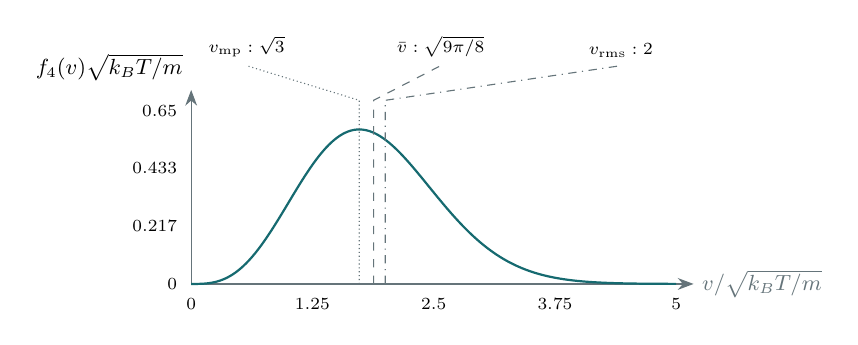
\begin{tikzpicture}[scale=.88,transform shape]
\draw[axis] (0,0.0000000)--(7.25,0.0000000) node[right] {$v/\sqrt{k_BT/m}$};
\draw[axis] (0.0000000,0)--(0.0000000,2.8);
\node[above left] at (0.0000000,2.8) {$f_4(v)\sqrt{k_BT/m}$};
\node[below,font=\scriptsize] at (0.0000000,-0.0800000) {$0$};
\node[below,font=\scriptsize] at (1.7500000,-0.0800000) {$1.25$};
\node[below,font=\scriptsize] at (3.5000000,-0.0800000) {$2.5$};
\node[below,font=\scriptsize] at (5.2500000,-0.0800000) {$3.75$};
\node[below,font=\scriptsize] at (7.0000000,-0.0800000) {$5$};
\node[left,font=\scriptsize] at (-0.0800000,0.0000000) {$0$};
\node[left,font=\scriptsize] at (-0.0800000,0.8333333) {$0.217$};
\node[left,font=\scriptsize] at (-0.0800000,1.6666667) {$0.433$};
\node[left,font=\scriptsize] at (-0.0800000,2.5000000) {$0.65$};
\draw[thick,color=accent] plot coordinates {(0.0000000,0.0000000) (0.0291667,0.0000174) (0.0583333,0.0001390) (0.0875000,0.0004686) (0.1166667,0.0011090) (0.1458333,0.0021619) (0.1750000,0.0037268) (0.2041667,0.0059013) (0.2333333,0.0087803) (0.2625000,0.0124556) (0.2916667,0.0170156) (0.3208333,0.0225448) (0.3500000,0.0291236) (0.3791667,0.0368277) (0.4083333,0.0457282) (0.4375000,0.0558909) (0.4666667,0.0673760) (0.4958333,0.0802384) (0.5250000,0.0945266) (0.5541667,0.1102834) (0.5833333,0.1275451) (0.6125000,0.1463415) (0.6416667,0.1666959) (0.6708333,0.1886250) (0.7000000,0.2121387) (0.7291667,0.2372401) (0.7583333,0.2639255) (0.7875000,0.2921847) (0.8166667,0.3220006) (0.8458333,0.3533495) (0.8750000,0.3862012) (0.9041667,0.4205191) (0.9333333,0.4562606) (0.9625000,0.4933768) (0.9916667,0.5318132) (1.0208333,0.5715094) (1.0500000,0.6123999) (1.0791667,0.6544142) (1.1083333,0.6974767) (1.1375000,0.7415077) (1.1666667,0.7864230) (1.1958333,0.8321349) (1.2250000,0.8785520) (1.2541667,0.9255798) (1.2833333,0.9731213) (1.3125000,1.0210768) (1.3416667,1.0693449) (1.3708333,1.1178225) (1.4000000,1.1664051) (1.4291667,1.2149877) (1.4583333,1.2634647) (1.4875000,1.3117304) (1.5166667,1.3596795) (1.5458333,1.4072074) (1.5750000,1.4542104) (1.6041667,1.5005864) (1.6333333,1.5462350) (1.6625000,1.5910579) (1.6916667,1.6349590) (1.7208333,1.6778453) (1.7500000,1.7196265) (1.7791667,1.7602157) (1.8083333,1.7995294) (1.8375000,1.8374881) (1.8666667,1.8740161) (1.8958333,1.9090420) (1.9250000,1.9424988) (1.9541667,1.9743238) (1.9833333,2.0044593) (2.0125000,2.0328522) (2.0416667,2.0594544) (2.0708333,2.0842228) (2.1000000,2.1071194) (2.1291667,2.1281110) (2.1583333,2.1471699) (2.1875000,2.1642733) (2.2166667,2.1794035) (2.2458333,2.1925480) (2.2750000,2.2036992) (2.3041667,2.2128545) (2.3333333,2.2200161) (2.3625000,2.2251910) (2.3916667,2.2283910) (2.4208333,2.2296321) (2.4500000,2.2289349) (2.4791667,2.2263241) (2.5083333,2.2218287) (2.5375000,2.2154813) (2.5666667,2.2073183) (2.5958333,2.1973795) (2.6250000,2.1857083) (2.6541667,2.1723509) (2.6833333,2.1573565) (2.7125000,2.1407769) (2.7416667,2.1226665) (2.7708333,2.1030817) (2.8000000,2.0820813) (2.8291667,2.0597254) (2.8583333,2.0360761) (2.8875000,2.0111966) (2.9166667,1.9851512) (2.9458333,1.9580054) (2.9750000,1.9298251) (3.0041667,1.9006768) (3.0333333,1.8706275) (3.0625000,1.8397439) (3.0916667,1.8080929) (3.1208333,1.7757412) (3.1500000,1.7427549) (3.1791667,1.7091994) (3.2083333,1.6751396) (3.2375000,1.6406392) (3.2666667,1.6057611) (3.2958333,1.5705668) (3.3250000,1.5351165) (3.3541667,1.4994691) (3.3833333,1.4636819) (3.4125000,1.4278104) (3.4416667,1.3919086) (3.4708333,1.3560285) (3.5000000,1.3202204) (3.5291667,1.2845324) (3.5583333,1.2490108) (3.5875000,1.2136998) (3.6166667,1.1786416) (3.6458333,1.1438762) (3.6750000,1.1094414) (3.7041667,1.0753731) (3.7333333,1.0417049) (3.7625000,1.0084682) (3.7916667,0.9756924) (3.8208333,0.9434047) (3.8500000,0.9116303) (3.8791667,0.8803921) (3.9083333,0.8497114) (3.9375000,0.8196070) (3.9666667,0.7900960) (3.9958333,0.7611937) (4.0250000,0.7329132) (4.0541667,0.7052661) (4.0833333,0.6782621) (4.1125000,0.6519092) (4.1416667,0.6262138) (4.1708333,0.6011807) (4.2000000,0.5768133) (4.2291667,0.5531133) (4.2583333,0.5300814) (4.2875000,0.5077166) (4.3166667,0.4860169) (4.3458333,0.4649790) (4.3750000,0.4445987) (4.4041667,0.4248706) (4.4333333,0.4057882) (4.4625000,0.3873445) (4.4916667,0.3695312) (4.5208333,0.3523396) (4.5500000,0.3357600) (4.5791667,0.3197824) (4.6083333,0.3043959) (4.6375000,0.2895892) (4.6666667,0.2753504) (4.6958333,0.2616675) (4.7250000,0.2485279) (4.7541667,0.2359187) (4.7833333,0.2238268) (4.8125000,0.2122388) (4.8416667,0.2011412) (4.8708333,0.1905205) (4.9000000,0.1803628) (4.9291667,0.1706545) (4.9583333,0.1613817) (4.9875000,0.1525308) (5.0166667,0.1440879) (5.0458333,0.1360394) (5.0750000,0.1283720) (5.1041667,0.1210721) (5.1333333,0.1141266) (5.1625000,0.1075225) (5.1916667,0.1012468) (5.2208333,0.0952871) (5.2500000,0.0896308) (5.2791667,0.0842659) (5.3083333,0.0791806) (5.3375000,0.0743630) (5.3666667,0.0698021) (5.3958333,0.0654866) (5.4250000,0.0614059) (5.4541667,0.0575495) (5.4833333,0.0539073) (5.5125000,0.0504694) (5.5416667,0.0472262) (5.5708333,0.0441687) (5.6000000,0.0412877) (5.6291667,0.0385748) (5.6583333,0.0360216) (5.6875000,0.0336201) (5.7166667,0.0313626) (5.7458333,0.0292418) (5.7750000,0.0272504) (5.8041667,0.0253816) (5.8333333,0.0236290) (5.8625000,0.0219862) (5.8916667,0.0204472) (5.9208333,0.0190063) (5.9500000,0.0176580) (5.9791667,0.0163970) (6.0083333,0.0152184) (6.0375000,0.0141174) (6.0666667,0.0130894) (6.0958333,0.0121302) (6.1250000,0.0112356) (6.1541667,0.0104018) (6.1833333,0.0096250) (6.2125000,0.0089018) (6.2416667,0.0082288) (6.2708333,0.0076029) (6.3000000,0.0070211) (6.3291667,0.0064805) (6.3583333,0.0059787) (6.3875000,0.0055129) (6.4166667,0.0050809) (6.4458333,0.0046804) (6.4750000,0.0043094) (6.5041667,0.0039658) (6.5333333,0.0036478) (6.5625000,0.0033537) (6.5916667,0.0030817) (6.6208333,0.0028304) (6.6500000,0.0025983) (6.6791667,0.0023841) (6.7083333,0.0021865) (6.7375000,0.0020042) (6.7666667,0.0018363) (6.7958333,0.0016816) (6.8250000,0.0015391) (6.8541667,0.0014081) (6.8833333,0.0012876) (6.9125000,0.0011768) (6.9416667,0.0010750) (6.9708333,0.0009816) (7.0000000,0.0008958)};
\draw[guide,densely dotted] (2.4248711,0)--(2.4248711,2.65)--(0.8,3.15);
\node[above,font=\scriptsize] at (0.8,3.15) {$v_{\rm mp}:\sqrt3$};
\draw[guide,dashed] (2.6319597,0)--(2.6319597,2.65)--(3.6,3.15);
\node[above,font=\scriptsize] at (3.6,3.15) {$\bar v:\sqrt{9\pi/8}$};
\draw[guide,dashdotted] (2.8000000,0)--(2.8000000,2.65)--(6.2,3.15);
\node[above,font=\scriptsize] at (6.2,3.15) {$v_{\rm rms}:2$};
\end{tikzpicture}
\figcaption{解图综一.3B\quad 归一化速率分布与三个典型速率}
\end{minipage}\end{center}
解图综一.3B中的分布在$v=0$为零，峰位、平均值和方均根对应三个不同位置。平均速率由
\[
\bar v=2b^2\int_0^\infty v^4e^{-bv^2}dv.
\]
一般积分用$x=bv^2$可得
\[
\int_0^\infty v^k e^{-bv^2}dv
=\frac{\Gamma[(k+1)/2]}{2b^{(k+1)/2}}.
\]
取$k=4$，利用$\Gamma(5/2)=\frac32\frac12\sqrt\pi$，
\[
\boxed{\bar v=\frac{3\sqrt\pi}{4\sqrt b}
=\frac{3\sqrt{2\pi}}4\sqrt{\frac{k_BT}{m}}
=\sqrt{\frac{9\pi k_BT}{8m}}}.
\]
四维平均速率积分中的$v^4e^{-bv^2}$也出现在三维气体的均方速率积分中。若以$f_3$表示同温、同质量的三维速率密度，则
\[
\int_0^\infty v^2f_3(v)\,\mathrm dv
=4\pi\left(\frac{m}{2\pi k_BT}\right)^{3/2}
\int_0^\infty v^4e^{-bv^2}\,\mathrm dv=\frac{3k_BT}{m}.
\]
将同一个积分代回四维平均速率，得到
\[
\bar v=\frac\pi2\left(\frac{m}{2\pi k_BT}\right)^{1/2}
\frac{3k_BT}{m}=\sqrt{\frac{9\pi k_BT}{8m}}.
\]
这说明维数变化后，同一个高斯径向积分会进入不同阶矩。上面的伽马函数方法给出任意阶矩，三维均方值则为这一个积分提供直接的物理解释。

由$f_4$求导还有$v_{\rm mp}=\sqrt{3k_BT/m}$，满足
$v_{\rm mp}<\bar v<v_{\rm rms}$，分别对应速率密度的峰值位置、速率的一阶矩与二阶矩的平方根。

法向为第一坐标方向的壁面只改变碰撞分子的第一速度分量。每次弹性反射传给壁的法向动量为$2m|v_1|$，单位时间内到达单位超面积的分子数又与$|v_1|$成正比。将朝向壁的一半分布相加，因分布关于$v_1=0$对称，得到$2\int_0^\infty mv_1^2F_1(v_1)\,\mathrm dv_1=m\langle v_1^2\rangle$。其他三个分量随其归一化积分约去，因此压强只取一个分量的均方值。

第（2a）问，取与第一坐标轴垂直的一面壁。分子碰壁的法向动量通量只包含$v_1$，同三维情形的碰撞计数给
\[
p=\frac{Nm}{V_4}\langle v_1^2\rangle
=\frac{N}{V_4}k_BT.
\]
于是
\[
\boxed{pV_4=Nk_BT=\nu RT}.
\]
若用$\epsilon_1=m\langle v_1^2\rangle/2$表示单分量平均动能，则$p=2(N/V_4)\epsilon_1$。压强使用单方向动能，内能则累加四个方向。

总内能与摩尔热容为
\[
U=2\nu RT,\qquad C_V=2R,\qquad C_p=C_V+R=3R.
\]
定压摩尔热容也可从第一定律逐项求出。在定压过程中，对$pV_4=\nu RT$微分有$p\,\mathrm dV_4=\nu R\,\mathrm dT$；内能增量为$2\nu R\,\mathrm dT$，两者相加给$\delta Q=3\nu R\,\mathrm dT$，所以$C_p=3R$。在准静态绝热过程中，内能增量$2\nu R\,\mathrm dT$与体积功$p\,\mathrm dV_4$之和为零；对一般路径，两者按该路径的$T,V_4$关系共同决定吸热量。

第（2b）问，准静态绝热过程满足
\[
0=dU+p\,dV_4
=\nu C_VdT+\nu RT\frac{dV_4}{V_4}.
\]
除以$\nu C_VT$并积分：
\[
\frac{dT}{T}+\frac{R}{C_V}\frac{dV_4}{V_4}=0
\ \Longrightarrow\ TV_4^{1/2}=\text{常量},
\]
再消去$T$，
\[
\boxed{pV_4^{3/2}=\text{常量}},\qquad \gamma=\frac32.
\]
\begin{center}\begin{minipage}{.98\linewidth}\centering
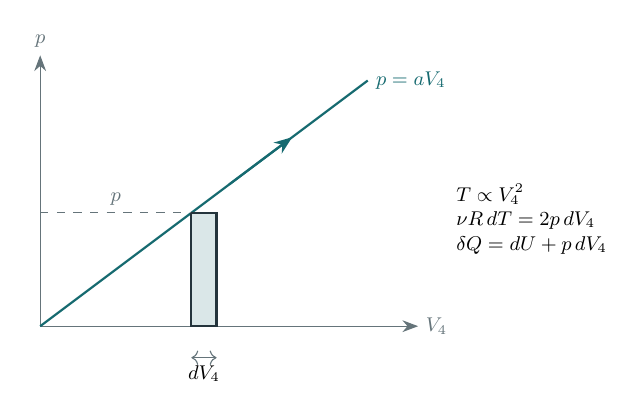
\begin{tikzpicture}[scale=.8,transform shape]

\draw[axis] (0,0)--(6,0) node[right] {$V_4$};
\draw[axis] (0,0)--(0,4.3) node[above] {$p$};
\draw[traj] (0,0)--(5.2,3.9) node[right] {$p=aV_4$};
\fill[accent!16] (2.4,0) rectangle (2.8,1.8);
\draw[object] (2.4,0) rectangle (2.8,1.8);
\draw[axis,<->] (2.4,-.5)--(2.8,-.5);
\node[below] at (2.6,-.5) {$dV_4$};
\draw[guide] (0,1.8)--(2.4,1.8) node[midway,above] {$p$};
\draw[motion] (3,2.25)--(4,3);
\node[align=left] at (7.8,1.7) {$T\propto V_4^2$\\$\nu R\,dT=2p\,dV_4$\\$\delta Q=dU+p\,dV_4$};

\end{tikzpicture}
\figcaption{解图综一.3C\quad 直线路径上的温升与体积功；两项相加求路径热容。}
\end{minipage}\end{center}
第（2c）问，解图综一.3C中的路径通过坐标原点，$p=aV_4$，斜率$a>0$，膨胀时压强随体积增加。由状态方程
\[
T=\frac{aV_4^2}{\nu R},\qquad
\nu R\,dT=2aV_4\,dV_4=2p\,dV_4.
\]
热力学第一定律给
\[
\delta Q=2\nu R\,dT+p\,dV_4
=\left(2+\frac12\right)\nu R\,dT,
\quad
\boxed{C=\frac{\delta Q}{\nu\,dT}=\frac52R}.
\]
沿这条路径膨胀时温度上升、吸热且对外做功。图中曲线下的面积正是$p\,dV_4$；沿路径的温升率把体积功换成每单位温升所需的热量。

对任一常摩尔热容$C$，有
\[
\nu(C-C_V)dT=p\,dV_4,\qquad
(C-C_V)\frac{dT}{T}=R\frac{dV_4}{V_4}.
\]
若$C\ne C_V$，结合$pV_4=\nu RT$，积分得到
\[
\boxed{pV_4^n=\text{常量},\qquad
n=1-\frac{R}{C-C_V}
=\frac{C-C_V-R}{C-C_V}}.
\]
本题$C-C_V=R/2$，所以$n=-1$，确为$p/V_4$恒定。$C=C_V$时由第一条微分关系得到$p\,dV_4=0$，对应等容过程，另用定容关系描述。
\begin{center}\begin{minipage}{.98\linewidth}\centering
\begin{tikzpicture}[scale=.88,transform shape]
\draw[axis] (0,0.0000000)--(7.25,0.0000000) node[right] {$V_4/V_i$};
\draw[axis] (0.0000000,0)--(0.0000000,2.8);
\node[above left] at (0.0000000,2.8) {$p/p_i$};
\node[below,font=\scriptsize] at (0.0000000,-0.0800000) {$0.5$};
\node[below,font=\scriptsize] at (1.7500000,-0.0800000) {$0.875$};
\node[below,font=\scriptsize] at (3.5000000,-0.0800000) {$1.25$};
\node[below,font=\scriptsize] at (5.2500000,-0.0800000) {$1.62$};
\node[below,font=\scriptsize] at (7.0000000,-0.0800000) {$2$};
\node[left,font=\scriptsize] at (-0.0800000,0.0000000) {$0$};
\node[left,font=\scriptsize] at (-0.0800000,0.8333333) {$1$};
\node[left,font=\scriptsize] at (-0.0800000,1.6666667) {$2$};
\node[left,font=\scriptsize] at (-0.0800000,2.5000000) {$3$};
\draw[thick,color=accent] plot coordinates {(0.0000000,0.4166667) (0.0291667,0.4218750) (0.0583333,0.4270833) (0.0875000,0.4322917) (0.1166667,0.4375000) (0.1458333,0.4427083) (0.1750000,0.4479167) (0.2041667,0.4531250) (0.2333333,0.4583333) (0.2625000,0.4635417) (0.2916667,0.4687500) (0.3208333,0.4739583) (0.3500000,0.4791667) (0.3791667,0.4843750) (0.4083333,0.4895833) (0.4375000,0.4947917) (0.4666667,0.5000000) (0.4958333,0.5052083) (0.5250000,0.5104167) (0.5541667,0.5156250) (0.5833333,0.5208333) (0.6125000,0.5260417) (0.6416667,0.5312500) (0.6708333,0.5364583) (0.7000000,0.5416667) (0.7291667,0.5468750) (0.7583333,0.5520833) (0.7875000,0.5572917) (0.8166667,0.5625000) (0.8458333,0.5677083) (0.8750000,0.5729167) (0.9041667,0.5781250) (0.9333333,0.5833333) (0.9625000,0.5885417) (0.9916667,0.5937500) (1.0208333,0.5989583) (1.0500000,0.6041667) (1.0791667,0.6093750) (1.1083333,0.6145833) (1.1375000,0.6197917) (1.1666667,0.6250000) (1.1958333,0.6302083) (1.2250000,0.6354167) (1.2541667,0.6406250) (1.2833333,0.6458333) (1.3125000,0.6510417) (1.3416667,0.6562500) (1.3708333,0.6614583) (1.4000000,0.6666667) (1.4291667,0.6718750) (1.4583333,0.6770833) (1.4875000,0.6822917) (1.5166667,0.6875000) (1.5458333,0.6927083) (1.5750000,0.6979167) (1.6041667,0.7031250) (1.6333333,0.7083333) (1.6625000,0.7135417) (1.6916667,0.7187500) (1.7208333,0.7239583) (1.7500000,0.7291667) (1.7791667,0.7343750) (1.8083333,0.7395833) (1.8375000,0.7447917) (1.8666667,0.7500000) (1.8958333,0.7552083) (1.9250000,0.7604167) (1.9541667,0.7656250) (1.9833333,0.7708333) (2.0125000,0.7760417) (2.0416667,0.7812500) (2.0708333,0.7864583) (2.1000000,0.7916667) (2.1291667,0.7968750) (2.1583333,0.8020833) (2.1875000,0.8072917) (2.2166667,0.8125000) (2.2458333,0.8177083) (2.2750000,0.8229167) (2.3041667,0.8281250) (2.3333333,0.8333333) (2.3625000,0.8385417) (2.3916667,0.8437500) (2.4208333,0.8489583) (2.4500000,0.8541667) (2.4791667,0.8593750) (2.5083333,0.8645833) (2.5375000,0.8697917) (2.5666667,0.8750000) (2.5958333,0.8802083) (2.6250000,0.8854167) (2.6541667,0.8906250) (2.6833333,0.8958333) (2.7125000,0.9010417) (2.7416667,0.9062500) (2.7708333,0.9114583) (2.8000000,0.9166667) (2.8291667,0.9218750) (2.8583333,0.9270833) (2.8875000,0.9322917) (2.9166667,0.9375000) (2.9458333,0.9427083) (2.9750000,0.9479167) (3.0041667,0.9531250) (3.0333333,0.9583333) (3.0625000,0.9635417) (3.0916667,0.9687500) (3.1208333,0.9739583) (3.1500000,0.9791667) (3.1791667,0.9843750) (3.2083333,0.9895833) (3.2375000,0.9947917) (3.2666667,1.0000000) (3.2958333,1.0052083) (3.3250000,1.0104167) (3.3541667,1.0156250) (3.3833333,1.0208333) (3.4125000,1.0260417) (3.4416667,1.0312500) (3.4708333,1.0364583) (3.5000000,1.0416667) (3.5291667,1.0468750) (3.5583333,1.0520833) (3.5875000,1.0572917) (3.6166667,1.0625000) (3.6458333,1.0677083) (3.6750000,1.0729167) (3.7041667,1.0781250) (3.7333333,1.0833333) (3.7625000,1.0885417) (3.7916667,1.0937500) (3.8208333,1.0989583) (3.8500000,1.1041667) (3.8791667,1.1093750) (3.9083333,1.1145833) (3.9375000,1.1197917) (3.9666667,1.1250000) (3.9958333,1.1302083) (4.0250000,1.1354167) (4.0541667,1.1406250) (4.0833333,1.1458333) (4.1125000,1.1510417) (4.1416667,1.1562500) (4.1708333,1.1614583) (4.2000000,1.1666667) (4.2291667,1.1718750) (4.2583333,1.1770833) (4.2875000,1.1822917) (4.3166667,1.1875000) (4.3458333,1.1927083) (4.3750000,1.1979167) (4.4041667,1.2031250) (4.4333333,1.2083333) (4.4625000,1.2135417) (4.4916667,1.2187500) (4.5208333,1.2239583) (4.5500000,1.2291667) (4.5791667,1.2343750) (4.6083333,1.2395833) (4.6375000,1.2447917) (4.6666667,1.2500000) (4.6958333,1.2552083) (4.7250000,1.2604167) (4.7541667,1.2656250) (4.7833333,1.2708333) (4.8125000,1.2760417) (4.8416667,1.2812500) (4.8708333,1.2864583) (4.9000000,1.2916667) (4.9291667,1.2968750) (4.9583333,1.3020833) (4.9875000,1.3072917) (5.0166667,1.3125000) (5.0458333,1.3177083) (5.0750000,1.3229167) (5.1041667,1.3281250) (5.1333333,1.3333333) (5.1625000,1.3385417) (5.1916667,1.3437500) (5.2208333,1.3489583) (5.2500000,1.3541667) (5.2791667,1.3593750) (5.3083333,1.3645833) (5.3375000,1.3697917) (5.3666667,1.3750000) (5.3958333,1.3802083) (5.4250000,1.3854167) (5.4541667,1.3906250) (5.4833333,1.3958333) (5.5125000,1.4010417) (5.5416667,1.4062500) (5.5708333,1.4114583) (5.6000000,1.4166667) (5.6291667,1.4218750) (5.6583333,1.4270833) (5.6875000,1.4322917) (5.7166667,1.4375000) (5.7458333,1.4427083) (5.7750000,1.4479167) (5.8041667,1.4531250) (5.8333333,1.4583333) (5.8625000,1.4635417) (5.8916667,1.4687500) (5.9208333,1.4739583) (5.9500000,1.4791667) (5.9791667,1.4843750) (6.0083333,1.4895833) (6.0375000,1.4947917) (6.0666667,1.5000000) (6.0958333,1.5052083) (6.1250000,1.5104167) (6.1541667,1.5156250) (6.1833333,1.5208333) (6.2125000,1.5260417) (6.2416667,1.5312500) (6.2708333,1.5364583) (6.3000000,1.5416667) (6.3291667,1.5468750) (6.3583333,1.5520833) (6.3875000,1.5572917) (6.4166667,1.5625000) (6.4458333,1.5677083) (6.4750000,1.5729167) (6.5041667,1.5781250) (6.5333333,1.5833333) (6.5625000,1.5885417) (6.5916667,1.5937500) (6.6208333,1.5989583) (6.6500000,1.6041667) (6.6791667,1.6093750) (6.7083333,1.6145833) (6.7375000,1.6197917) (6.7666667,1.6250000) (6.7958333,1.6302083) (6.8250000,1.6354167) (6.8541667,1.6406250) (6.8833333,1.6458333) (6.9125000,1.6510417) (6.9416667,1.6562500) (6.9708333,1.6614583) (7.0000000,1.6666667)};
\draw[thick,color=accent] (7.65,2.4)--(8.1,2.4);\node[right,font=\scriptsize] at (8.15,2.4) {$p\propto V_4$};
\draw[thick,dashed,color=warm] plot coordinates {(0.0000000,2.3570226) (0.0291667,2.3135090) (0.0583333,2.2713180) (0.0875000,2.2303940) (0.1166667,2.1906843) (0.1458333,2.1521391) (0.1750000,2.1147111) (0.2041667,2.0783556) (0.2333333,2.0430299) (0.2625000,2.0086937) (0.2916667,1.9753086) (0.3208333,1.9428382) (0.3500000,1.9112477) (0.3791667,1.8805042) (0.4083333,1.8505761) (0.4375000,1.8214335) (0.4666667,1.7930478) (0.4958333,1.7653919) (0.5250000,1.7384396) (0.5541667,1.7121663) (0.5833333,1.6865481) (0.6125000,1.6615624) (0.6416667,1.6371877) (0.6708333,1.6134031) (0.7000000,1.5901889) (0.7291667,1.5675261) (0.7583333,1.5453965) (0.7875000,1.5237828) (0.8166667,1.5026682) (0.8458333,1.4820368) (0.8750000,1.4618732) (0.9041667,1.4421627) (0.9333333,1.4228912) (0.9625000,1.4040451) (0.9916667,1.3856114) (1.0208333,1.3675776) (1.0500000,1.3499315) (1.0791667,1.3326618) (1.1083333,1.3157571) (1.1375000,1.2992068) (1.1666667,1.2830006) (1.1958333,1.2671285) (1.2250000,1.2515811) (1.2541667,1.2363489) (1.2833333,1.2214233) (1.3125000,1.2067956) (1.3416667,1.1924575) (1.3708333,1.1784011) (1.4000000,1.1646187) (1.4291667,1.1511029) (1.4583333,1.1378466) (1.4875000,1.1248427) (1.5166667,1.1120846) (1.5458333,1.0995659) (1.5750000,1.0872803) (1.6041667,1.0752218) (1.6333333,1.0633846) (1.6625000,1.0517630) (1.6916667,1.0403515) (1.7208333,1.0291449) (1.7500000,1.0181381) (1.7791667,1.0073260) (1.8083333,0.9967040) (1.8375000,0.9862674) (1.8666667,0.9760116) (1.8958333,0.9659324) (1.9250000,0.9560254) (1.9541667,0.9462867) (1.9833333,0.9367122) (2.0125000,0.9272980) (2.0416667,0.9180405) (2.0708333,0.9089360) (2.1000000,0.8999810) (2.1291667,0.8911721) (2.1583333,0.8825060) (2.1875000,0.8739794) (2.2166667,0.8655892) (2.2458333,0.8573324) (2.2750000,0.8492061) (2.3041667,0.8412073) (2.3333333,0.8333333) (2.3625000,0.8255814) (2.3916667,0.8179490) (2.4208333,0.8104334) (2.4500000,0.8030322) (2.4791667,0.7957430) (2.5083333,0.7885634) (2.5375000,0.7814911) (2.5666667,0.7745239) (2.5958333,0.7676596) (2.6250000,0.7608961) (2.6541667,0.7542313) (2.6833333,0.7476633) (2.7125000,0.7411900) (2.7416667,0.7348097) (2.7708333,0.7285203) (2.8000000,0.7223201) (2.8291667,0.7162074) (2.8583333,0.7101805) (2.8875000,0.7042376) (2.9166667,0.6983771) (2.9458333,0.6925974) (2.9750000,0.6868970) (3.0041667,0.6812744) (3.0333333,0.6757281) (3.0625000,0.6702567) (3.0916667,0.6648586) (3.1208333,0.6595327) (3.1500000,0.6542775) (3.1791667,0.6490916) (3.2083333,0.6439740) (3.2375000,0.6389232) (3.2666667,0.6339381) (3.2958333,0.6290176) (3.3250000,0.6241603) (3.3541667,0.6193652) (3.3833333,0.6146312) (3.4125000,0.6099572) (3.4416667,0.6053422) (3.4708333,0.6007850) (3.5000000,0.5962848) (3.5291667,0.5918404) (3.5583333,0.5874510) (3.5875000,0.5831156) (3.6166667,0.5788333) (3.6458333,0.5746031) (3.6750000,0.5704241) (3.7041667,0.5662956) (3.7333333,0.5622167) (3.7625000,0.5581865) (3.7916667,0.5542042) (3.8208333,0.5502690) (3.8500000,0.5463802) (3.8791667,0.5425370) (3.9083333,0.5387386) (3.9375000,0.5349843) (3.9666667,0.5312734) (3.9958333,0.5276053) (4.0250000,0.5239791) (4.0541667,0.5203943) (4.0833333,0.5168502) (4.1125000,0.5133462) (4.1416667,0.5098815) (4.1708333,0.5064557) (4.2000000,0.5030680) (4.2291667,0.4997180) (4.2583333,0.4964049) (4.2875000,0.4931283) (4.3166667,0.4898876) (4.3458333,0.4866822) (4.3750000,0.4835117) (4.4041667,0.4803754) (4.4333333,0.4772729) (4.4625000,0.4742036) (4.4916667,0.4711671) (4.5208333,0.4681628) (4.5500000,0.4651904) (4.5791667,0.4622492) (4.6083333,0.4593390) (4.6375000,0.4564591) (4.6666667,0.4536092) (4.6958333,0.4507888) (4.7250000,0.4479976) (4.7541667,0.4452350) (4.7833333,0.4425007) (4.8125000,0.4397943) (4.8416667,0.4371154) (4.8708333,0.4344635) (4.9000000,0.4318383) (4.9291667,0.4292395) (4.9583333,0.4266667) (4.9875000,0.4241194) (5.0166667,0.4215974) (5.0458333,0.4191003) (5.0750000,0.4166277) (5.1041667,0.4141794) (5.1333333,0.4117549) (5.1625000,0.4093540) (5.1916667,0.4069763) (5.2208333,0.4046216) (5.2500000,0.4022895) (5.2791667,0.3999797) (5.3083333,0.3976919) (5.3375000,0.3954259) (5.3666667,0.3931813) (5.3958333,0.3909578) (5.4250000,0.3887553) (5.4541667,0.3865733) (5.4833333,0.3844116) (5.5125000,0.3822701) (5.5416667,0.3801483) (5.5708333,0.3780461) (5.6000000,0.3759632) (5.6291667,0.3738994) (5.6583333,0.3718544) (5.6875000,0.3698279) (5.7166667,0.3678198) (5.7458333,0.3658298) (5.7750000,0.3638577) (5.8041667,0.3619032) (5.8333333,0.3599662) (5.8625000,0.3580463) (5.8916667,0.3561435) (5.9208333,0.3542575) (5.9500000,0.3523881) (5.9791667,0.3505350) (6.0083333,0.3486982) (6.0375000,0.3468773) (6.0666667,0.3450722) (6.0958333,0.3432827) (6.1250000,0.3415087) (6.1541667,0.3397498) (6.1833333,0.3380060) (6.2125000,0.3362771) (6.2416667,0.3345629) (6.2708333,0.3328631) (6.3000000,0.3311778) (6.3291667,0.3295066) (6.3583333,0.3278494) (6.3875000,0.3262060) (6.4166667,0.3245763) (6.4458333,0.3229602) (6.4750000,0.3213574) (6.5041667,0.3197678) (6.5333333,0.3181913) (6.5625000,0.3166277) (6.5916667,0.3150769) (6.6208333,0.3135387) (6.6500000,0.3120130) (6.6791667,0.3104996) (6.7083333,0.3089984) (6.7375000,0.3075092) (6.7666667,0.3060320) (6.7958333,0.3045666) (6.8250000,0.3031128) (6.8541667,0.3016705) (6.8833333,0.3002397) (6.9125000,0.2988201) (6.9416667,0.2974117) (6.9708333,0.2960143) (7.0000000,0.2946278)};
\draw[thick,dashed,color=warm] (7.65,1.9)--(8.1,1.9);\node[right,font=\scriptsize] at (8.15,1.9) {$pV_4^{3/2}=\text{常量}$};
\end{tikzpicture}
\figcaption{解图综一.3D\quad 通过同一状态的升压直线与绝热曲线}
\end{minipage}\end{center}
解图综一.3D把同一状态出发的$p\propto V_4$路径与绝热路径放在一起。前者膨胀时压强、温度同时升高，吸热既补充内能，又提供体积功；后者膨胀时温度下降，做功来自内能的减少。两条曲线的不同斜率直接对应不同的温度变化率，所以路径热容由具体的过程方程计算。



\Needspace{8\baselineskip}

\pdfbookmark[3]{关键洞察}{q3-h5}

\subsection*{关键洞察}

压强测量一个法向分量的动量通量，状态方程保持$pV_4=\nu RT$的形式；总内能累加四个分量，所以$C_V=2R$。速度矢量密度与速率密度相差整层方向态的数量，即$2\pi^2v^3$。常热容由沿过程的温升率定义，因而$p\propto V_4$的热容为$5R/2$，位于$C_V$和$C_p$之间。

\Needspace{8\baselineskip}

\pdfbookmark[3]{易错点}{q3-h6}

\subsection*{易错点}

\begin{itemize}
\item 速率壳使用$2\pi^2v^3\,\mathrm dv$，其几何维数与联合密度的四个微分分量对应。
\item 纬带厚度沿子午线取$a\,\mathrm d\varphi$；第四坐标投影是另一种长度。
\item 壁面动量通量使用$\langle v_1^2\rangle$，内能使用$\sum_i\langle v_i^2\rangle$。
\item 从状态方程沿给定路径微分，先算出温升与体积功的比例，再求热容。
\item 一般多方指数在$C\ne C_V$时使用；$C=C_V$直接由微分热量关系给等容过程。
\end{itemize}

\Needspace{8\baselineskip}

\pdfbookmark[3]{课堂讲解建议}{q3-h7}

\subsection*{课堂讲解建议}

先并列三维与四维的联合密度、壳面积、速率密度三列，请学生说明每列改变的依据。画图A时问：“固定极角的截面是什么？纬带宽度沿哪条线量？”分别回答二维球面和子午弧。积分后用球体积求导说明同一超面积。讲状态方程时问：“法向为第一轴的壁面记录哪一项动量变化？”由碰壁只反转$v_1$得到单分量压强，再与四分量内能并列。最后取图C的一小段，让学生分别计算内能增量与体积功，相加得到$5R/2$；在图D指出绝热膨胀的温度变化为何不同。

\Needspace{8\baselineskip}

\pdfbookmark[3]{变式训练}{q3-h8}

\subsection*{变式训练}

\begin{enumerate}
\item \textbf{推广到$d$维速率分布。} 设$d$个速度分量独立且具有相同高斯方差，求速率密度、平均速率和方均根速率。
\par 半径$v$的速度壳超面积为$2\pi^{d/2}v^{d-1}/\Gamma(d/2)$，联合密度为$[m/(2\pi k_BT)]^{d/2}e^{-mv^2/(2k_BT)}$。相乘并用$b=m/(2k_BT)$，得
\[
f_d(v)=\frac{2b^{d/2}}{\Gamma(d/2)}v^{d-1}e^{-bv^2},\quad
\langle v^q\rangle=b^{-q/2}\frac{\Gamma[(d+q)/2]}{\Gamma(d/2)},\qquad q>-d.
\]
\begin{center}\begin{minipage}{.98\linewidth}\centering
\begin{tikzpicture}[scale=.88,transform shape]
\draw[axis] (0,0.0000000)--(7.25,0.0000000) node[right] {$v/\sqrt{k_BT/m}$};
\draw[axis] (0.0000000,0)--(0.0000000,2.8);
\node[above left] at (0.0000000,2.8) {$\text{无量纲密度}$};
\node[below,font=\scriptsize] at (0.0000000,-0.0800000) {$0$};
\node[below,font=\scriptsize] at (1.7500000,-0.0800000) {$1.25$};
\node[below,font=\scriptsize] at (3.5000000,-0.0800000) {$2.5$};
\node[below,font=\scriptsize] at (5.2500000,-0.0800000) {$3.75$};
\node[below,font=\scriptsize] at (7.0000000,-0.0800000) {$5$};
\node[left,font=\scriptsize] at (-0.0800000,0.0000000) {$0$};
\node[left,font=\scriptsize] at (-0.0800000,0.8333333) {$0.233$};
\node[left,font=\scriptsize] at (-0.0800000,1.6666667) {$0.467$};
\node[left,font=\scriptsize] at (-0.0800000,2.5000000) {$0.7$};
\draw[thick,color=accent] plot coordinates {(0.0000000,0.0000000) (0.0291667,0.0743886) (0.0583333,0.1486804) (0.0875000,0.2227787) (0.1166667,0.2965874) (0.1458333,0.3700109) (0.1750000,0.4429544) (0.2041667,0.5153243) (0.2333333,0.5870280) (0.2625000,0.6579746) (0.2916667,0.7280747) (0.3208333,0.7972406) (0.3500000,0.8653868) (0.3791667,0.9324299) (0.4083333,0.9982887) (0.4375000,1.0628848) (0.4666667,1.1261422) (0.4958333,1.1879879) (0.5250000,1.2483516) (0.5541667,1.3071663) (0.5833333,1.3643681) (0.6125000,1.4198965) (0.6416667,1.4736943) (0.6708333,1.5257080) (0.7000000,1.5758873) (0.7291667,1.6241861) (0.7583333,1.6705615) (0.7875000,1.7149748) (0.8166667,1.7573909) (0.8458333,1.7977786) (0.8750000,1.8361106) (0.9041667,1.8723635) (0.9333333,1.9065176) (0.9625000,1.9385574) (0.9916667,1.9684711) (1.0208333,1.9962506) (1.0500000,2.0218918) (1.0791667,2.0453943) (1.1083333,2.0667613) (1.1375000,2.0859996) (1.1666667,2.1031199) (1.1958333,2.1181358) (1.2250000,2.1310648) (1.2541667,2.1419274) (1.2833333,2.1507474) (1.3125000,2.1575515) (1.3416667,2.1623696) (1.3708333,2.1652343) (1.4000000,2.1661809) (1.4291667,2.1652474) (1.4583333,2.1624740) (1.4875000,2.1579036) (1.5166667,2.1515808) (1.5458333,2.1435526) (1.5750000,2.1338678) (1.6041667,2.1225768) (1.6333333,2.1097317) (1.6625000,2.0953860) (1.6916667,2.0795946) (1.7208333,2.0624132) (1.7500000,2.0438989) (1.7791667,2.0241095) (1.8083333,2.0031034) (1.8375000,1.9809396) (1.8666667,1.9576776) (1.8958333,1.9333771) (1.9250000,1.9080979) (1.9541667,1.8819001) (1.9833333,1.8548432) (2.0125000,1.8269868) (2.0416667,1.7983901) (2.0708333,1.7691117) (2.1000000,1.7392096) (2.1291667,1.7087414) (2.1583333,1.6777636) (2.1875000,1.6463318) (2.2166667,1.6145008) (2.2458333,1.5823241) (2.2750000,1.5498544) (2.3041667,1.5171428) (2.3333333,1.4842393) (2.3625000,1.4511926) (2.3916667,1.4180498) (2.4208333,1.3848566) (2.4500000,1.3516573) (2.4791667,1.3184945) (2.5083333,1.2854094) (2.5375000,1.2524413) (2.5666667,1.2196280) (2.5958333,1.1870058) (2.6250000,1.1546091) (2.6541667,1.1224706) (2.6833333,1.0906215) (2.7125000,1.0590910) (2.7416667,1.0279070) (2.7708333,0.9970954) (2.8000000,0.9666806) (2.8291667,0.9366852) (2.8583333,0.9071302) (2.8875000,0.8780352) (2.9166667,0.8494179) (2.9458333,0.8212945) (2.9750000,0.7936799) (3.0041667,0.7665873) (3.0333333,0.7400284) (3.0625000,0.7140137) (3.0916667,0.6885521) (3.1208333,0.6636512) (3.1500000,0.6393175) (3.1791667,0.6155559) (3.2083333,0.5923705) (3.2375000,0.5697639) (3.2666667,0.5477377) (3.2958333,0.5262926) (3.3250000,0.5054282) (3.3541667,0.4851429) (3.3833333,0.4654344) (3.4125000,0.4462997) (3.4416667,0.4277347) (3.4708333,0.4097347) (3.5000000,0.3922941) (3.5291667,0.3754068) (3.5583333,0.3590660) (3.5875000,0.3432645) (3.6166667,0.3279942) (3.6458333,0.3132469) (3.6750000,0.2990137) (3.7041667,0.2852854) (3.7333333,0.2720524) (3.7625000,0.2593048) (3.7916667,0.2470324) (3.8208333,0.2352249) (3.8500000,0.2238714) (3.8791667,0.2129613) (3.9083333,0.2024835) (3.9375000,0.1924269) (3.9666667,0.1827805) (3.9958333,0.1735329) (4.0250000,0.1646729) (4.0541667,0.1561893) (4.0833333,0.1480707) (4.1125000,0.1403061) (4.1416667,0.1328843) (4.1708333,0.1257942) (4.2000000,0.1190250) (4.2291667,0.1125657) (4.2583333,0.1064056) (4.2875000,0.1005343) (4.3166667,0.0949414) (4.3458333,0.0896166) (4.3750000,0.0845500) (4.4041667,0.0797316) (4.4333333,0.0751519) (4.4625000,0.0708015) (4.4916667,0.0666711) (4.5208333,0.0627517) (4.5500000,0.0590347) (4.5791667,0.0555115) (4.6083333,0.0521738) (4.6375000,0.0490135) (4.6666667,0.0460229) (4.6958333,0.0431942) (4.7250000,0.0405203) (4.7541667,0.0379940) (4.7833333,0.0356084) (4.8125000,0.0333568) (4.8416667,0.0312329) (4.8708333,0.0292305) (4.9000000,0.0273436) (4.9291667,0.0255666) (4.9583333,0.0238938) (4.9875000,0.0223199) (5.0166667,0.0208400) (5.0458333,0.0194491) (5.0750000,0.0181426) (5.1041667,0.0169159) (5.1333333,0.0157648) (5.1625000,0.0146852) (5.1916667,0.0136732) (5.2208333,0.0127249) (5.2500000,0.0118370) (5.2791667,0.0110058) (5.3083333,0.0102283) (5.3375000,0.0095013) (5.3666667,0.0088219) (5.3958333,0.0081872) (5.4250000,0.0075947) (5.4541667,0.0070418) (5.4833333,0.0065262) (5.5125000,0.0060455) (5.5416667,0.0055976) (5.5708333,0.0051805) (5.6000000,0.0047923) (5.6291667,0.0044312) (5.6583333,0.0040953) (5.6875000,0.0037832) (5.7166667,0.0034932) (5.7458333,0.0032240) (5.7750000,0.0029742) (5.8041667,0.0027425) (5.8333333,0.0025276) (5.8625000,0.0023286) (5.8916667,0.0021442) (5.9208333,0.0019735) (5.9500000,0.0018156) (5.9791667,0.0016695) (6.0083333,0.0015345) (6.0375000,0.0014097) (6.0666667,0.0012946) (6.0958333,0.0011882) (6.1250000,0.0010901) (6.1541667,0.0009997) (6.1833333,0.0009163) (6.2125000,0.0008395) (6.2416667,0.0007688) (6.2708333,0.0007038) (6.3000000,0.0006439) (6.3291667,0.0005889) (6.3583333,0.0005383) (6.3875000,0.0004918) (6.4166667,0.0004492) (6.4458333,0.0004100) (6.4750000,0.0003741) (6.5041667,0.0003412) (6.5333333,0.0003111) (6.5625000,0.0002835) (6.5916667,0.0002582) (6.6208333,0.0002350) (6.6500000,0.0002139) (6.6791667,0.0001945) (6.7083333,0.0001769) (6.7375000,0.0001607) (6.7666667,0.0001460) (6.7958333,0.0001325) (6.8250000,0.0001203) (6.8541667,0.0001091) (6.8833333,0.0000989) (6.9125000,0.0000896) (6.9416667,0.0000812) (6.9708333,0.0000735) (7.0000000,0.0000665)};
\draw[thick,color=accent] (7.65,2.4)--(8.1,2.4);\node[right,font=\scriptsize] at (8.15,2.4) {$d=2$};
\draw[thick,dashed,color=warm] plot coordinates {(0.0000000,0.0000000) (0.0291667,0.0012365) (0.0583333,0.0049429) (0.0875000,0.0111095) (0.1166667,0.0197202) (0.1458333,0.0307527) (0.1750000,0.0441783) (0.2041667,0.0599622) (0.2333333,0.0780634) (0.2625000,0.0984352) (0.2916667,0.1210249) (0.3208333,0.1457743) (0.3500000,0.1726197) (0.3791667,0.2014923) (0.4083333,0.2323181) (0.4375000,0.2650186) (0.4666667,0.2995105) (0.4958333,0.3357065) (0.5250000,0.3735152) (0.5541667,0.4128414) (0.5833333,0.4535868) (0.6125000,0.4956497) (0.6416667,0.5389257) (0.6708333,0.5833082) (0.7000000,0.6286881) (0.7291667,0.6749547) (0.7583333,0.7219958) (0.7875000,0.7696980) (0.8166667,0.8179471) (0.8458333,0.8666286) (0.8750000,0.9156277) (0.9041667,0.9648297) (0.9333333,1.0141207) (0.9625000,1.0633872) (0.9916667,1.1125173) (1.0208333,1.1614003) (1.0500000,1.2099272) (1.0791667,1.2579911) (1.1083333,1.3054875) (1.1375000,1.3523144) (1.1666667,1.3983724) (1.1958333,1.4435655) (1.2250000,1.4878008) (1.2541667,1.5309889) (1.2833333,1.5730441) (1.3125000,1.6138847) (1.3416667,1.6534330) (1.3708333,1.6916152) (1.4000000,1.7283623) (1.4291667,1.7636095) (1.4583333,1.7972965) (1.4875000,1.8293678) (1.5166667,1.8597725) (1.5458333,1.8884646) (1.5750000,1.9154027) (1.6041667,1.9405504) (1.6333333,1.9638761) (1.6625000,1.9853530) (1.6916667,2.0049590) (1.7208333,2.0226769) (1.7500000,2.0384943) (1.7791667,2.0524031) (1.8083333,2.0644001) (1.8375000,2.0744865) (1.8666667,2.0826676) (1.8958333,2.0889534) (1.9250000,2.0933576) (1.9541667,2.0958982) (1.9833333,2.0965969) (2.0125000,2.0954790) (2.0416667,2.0925737) (2.0708333,2.0879131) (2.1000000,2.0815328) (2.1291667,2.0734713) (2.1583333,2.0637701) (2.1875000,2.0524730) (2.2166667,2.0396266) (2.2458333,2.0252797) (2.2750000,2.0094830) (2.3041667,1.9922892) (2.3333333,1.9737528) (2.3625000,1.9539295) (2.3916667,1.9328767) (2.4208333,1.9106526) (2.4500000,1.8873163) (2.4791667,1.8629280) (2.5083333,1.8375482) (2.5375000,1.8112377) (2.5666667,1.7840577) (2.5958333,1.7560694) (2.6250000,1.7273339) (2.6541667,1.6979121) (2.6833333,1.6678642) (2.7125000,1.6372503) (2.7416667,1.6061293) (2.7708333,1.5745598) (2.8000000,1.5425990) (2.8291667,1.5103034) (2.8583333,1.4777281) (2.8875000,1.4449271) (2.9166667,1.4119529) (2.9458333,1.3788567) (2.9750000,1.3456880) (3.0041667,1.3124950) (3.0333333,1.2793241) (3.0625000,1.2462199) (3.0916667,1.2132254) (3.1208333,1.1803818) (3.1500000,1.1477285) (3.1791667,1.1153029) (3.2083333,1.0831408) (3.2375000,1.0512759) (3.2666667,1.0197401) (3.2958333,0.9885635) (3.3250000,0.9577741) (3.3541667,0.9273983) (3.3833333,0.8974605) (3.4125000,0.8679832) (3.4416667,0.8389872) (3.4708333,0.8104915) (3.5000000,0.7825134) (3.5291667,0.7550684) (3.5583333,0.7281703) (3.5875000,0.7018314) (3.6166667,0.6760622) (3.6458333,0.6508720) (3.6750000,0.6262683) (3.7041667,0.6022573) (3.7333333,0.5788437) (3.7625000,0.5560311) (3.7916667,0.5338216) (3.8208333,0.5122162) (3.8500000,0.4912148) (3.8791667,0.4708159) (3.9083333,0.4510173) (3.9375000,0.4318158) (3.9666667,0.4132069) (3.9958333,0.3951857) (4.0250000,0.3777462) (4.0541667,0.3608817) (4.0833333,0.3445848) (4.1125000,0.3288475) (4.1416667,0.3136613) (4.1708333,0.2990168) (4.2000000,0.2849045) (4.2291667,0.2713143) (4.2583333,0.2582357) (4.2875000,0.2456578) (4.3166667,0.2335696) (4.3458333,0.2219595) (4.3750000,0.2108160) (4.4041667,0.2001273) (4.4333333,0.1898814) (4.4625000,0.1800663) (4.4916667,0.1706699) (4.5208333,0.1616800) (4.5500000,0.1530844) (4.5791667,0.1448710) (4.6083333,0.1370277) (4.6375000,0.1295424) (4.6666667,0.1224031) (4.6958333,0.1155981) (4.7250000,0.1091156) (4.7541667,0.1029441) (4.7833333,0.0970722) (4.8125000,0.0914887) (4.8416667,0.0861826) (4.8708333,0.0811431) (4.9000000,0.0763597) (4.9291667,0.0718220) (4.9583333,0.0675199) (4.9875000,0.0634436) (5.0166667,0.0595834) (5.0458333,0.0559301) (5.0750000,0.0524744) (5.1041667,0.0492077) (5.1333333,0.0461212) (5.1625000,0.0432068) (5.1916667,0.0404565) (5.2208333,0.0378623) (5.2500000,0.0354170) (5.2791667,0.0331131) (5.3083333,0.0309438) (5.3375000,0.0289023) (5.3666667,0.0269822) (5.3958333,0.0251772) (5.4250000,0.0234814) (5.4541667,0.0218890) (5.4833333,0.0203947) (5.5125000,0.0189930) (5.5416667,0.0176789) (5.5708333,0.0164478) (5.6000000,0.0152949) (5.6291667,0.0142159) (5.6583333,0.0132065) (5.6875000,0.0122628) (5.7166667,0.0113811) (5.7458333,0.0105576) (5.7750000,0.0097889) (5.8041667,0.0090718) (5.8333333,0.0084032) (5.8625000,0.0077800) (5.8916667,0.0071996) (5.9208333,0.0066593) (5.9500000,0.0061566) (5.9791667,0.0056890) (6.0083333,0.0052545) (6.0375000,0.0048508) (6.0666667,0.0044759) (6.0958333,0.0041281) (6.1250000,0.0038054) (6.1541667,0.0035063) (6.1833333,0.0032292) (6.2125000,0.0029725) (6.2416667,0.0027349) (6.2708333,0.0025152) (6.3000000,0.0023119) (6.3291667,0.0021241) (6.3583333,0.0019506) (6.3875000,0.0017905) (6.4166667,0.0016426) (6.4458333,0.0015063) (6.4750000,0.0013807) (6.5041667,0.0012649) (6.5333333,0.0011583) (6.5625000,0.0010601) (6.5916667,0.0009699) (6.6208333,0.0008868) (6.6500000,0.0008106) (6.6791667,0.0007405) (6.7083333,0.0006761) (6.7375000,0.0006171) (6.7666667,0.0005630) (6.7958333,0.0005133) (6.8250000,0.0004678) (6.8541667,0.0004262) (6.8833333,0.0003881) (6.9125000,0.0003532) (6.9416667,0.0003213) (6.9708333,0.0002921) (7.0000000,0.0002655)};
\draw[thick,dashed,color=warm] (7.65,1.9)--(8.1,1.9);\node[right,font=\scriptsize] at (8.15,1.9) {$d=3$};
\draw[thick,densely dotted,color=muted] plot coordinates {(0.0000000,0.0000000) (0.0291667,0.0000161) (0.0583333,0.0001291) (0.0875000,0.0004351) (0.1166667,0.0010298) (0.1458333,0.0020074) (0.1750000,0.0034606) (0.2041667,0.0054798) (0.2333333,0.0081532) (0.2625000,0.0115660) (0.2916667,0.0158002) (0.3208333,0.0209345) (0.3500000,0.0270433) (0.3791667,0.0341972) (0.4083333,0.0424619) (0.4375000,0.0518987) (0.4666667,0.0625635) (0.4958333,0.0745071) (0.5250000,0.0877747) (0.5541667,0.1024060) (0.5833333,0.1184347) (0.6125000,0.1358885) (0.6416667,0.1547891) (0.6708333,0.1751518) (0.7000000,0.1969859) (0.7291667,0.2202943) (0.7583333,0.2450737) (0.7875000,0.2713144) (0.8166667,0.2990005) (0.8458333,0.3281102) (0.8750000,0.3586154) (0.9041667,0.3904821) (0.9333333,0.4236706) (0.9625000,0.4581356) (0.9916667,0.4938265) (1.0208333,0.5306873) (1.0500000,0.5686571) (1.0791667,0.6076703) (1.1083333,0.6476570) (1.1375000,0.6885429) (1.1666667,0.7302500) (1.1958333,0.7726967) (1.2250000,0.8157983) (1.2541667,0.8594670) (1.2833333,0.9036126) (1.3125000,0.9481428) (1.3416667,0.9929631) (1.3708333,1.0379780) (1.4000000,1.0830905) (1.4291667,1.1282029) (1.4583333,1.1732172) (1.4875000,1.2180354) (1.5166667,1.2625596) (1.5458333,1.3066926) (1.5750000,1.3503382) (1.6041667,1.3934017) (1.6333333,1.4357897) (1.6625000,1.4774109) (1.6916667,1.5181762) (1.7208333,1.5579992) (1.7500000,1.5967960) (1.7791667,1.6344860) (1.8083333,1.6709916) (1.8375000,1.7062390) (1.8666667,1.7401578) (1.8958333,1.7726819) (1.9250000,1.8037488) (1.9541667,1.8333006) (1.9833333,1.8612836) (2.0125000,1.8876485) (2.0416667,1.9123505) (2.0708333,1.9353498) (2.1000000,1.9566109) (2.1291667,1.9761031) (2.1583333,1.9938006) (2.1875000,2.0096824) (2.2166667,2.0237319) (2.2458333,2.0359375) (2.2750000,2.0462921) (2.3041667,2.0547935) (2.3333333,2.0614435) (2.3625000,2.0662488) (2.3916667,2.0692202) (2.4208333,2.0703726) (2.4500000,2.0697252) (2.4791667,2.0673010) (2.5083333,2.0631267) (2.5375000,2.0572326) (2.5666667,2.0496527) (2.5958333,2.0404239) (2.6250000,2.0295863) (2.6541667,2.0171830) (2.6833333,2.0032596) (2.7125000,1.9878642) (2.7416667,1.9710474) (2.7708333,1.9528616) (2.8000000,1.9333612) (2.8291667,1.9126022) (2.8583333,1.8906421) (2.8875000,1.8675397) (2.9166667,1.8433547) (2.9458333,1.8181479) (2.9750000,1.7919804) (3.0041667,1.7649142) (3.0333333,1.7370112) (3.0625000,1.7083336) (3.0916667,1.6789434) (3.1208333,1.6489026) (3.1500000,1.6182724) (3.1791667,1.5871137) (3.2083333,1.5554867) (3.2375000,1.5234507) (3.2666667,1.4910638) (3.2958333,1.4583834) (3.3250000,1.4254653) (3.3541667,1.3923642) (3.3833333,1.3591332) (3.4125000,1.3258240) (3.4416667,1.2924866) (3.4708333,1.2591694) (3.5000000,1.2259189) (3.5291667,1.1927800) (3.5583333,1.1597957) (3.5875000,1.1270070) (3.6166667,1.0944529) (3.6458333,1.0621707) (3.6750000,1.0301956) (3.7041667,0.9985607) (3.7333333,0.9672974) (3.7625000,0.9364347) (3.7916667,0.9060001) (3.8208333,0.8760186) (3.8500000,0.8465138) (3.8791667,0.8175070) (3.9083333,0.7890177) (3.9375000,0.7610636) (3.9666667,0.7336606) (3.9958333,0.7068227) (4.0250000,0.6805623) (4.0541667,0.6548899) (4.0833333,0.6298148) (4.1125000,0.6053442) (4.1416667,0.5814842) (4.1708333,0.5582392) (4.2000000,0.5356123) (4.2291667,0.5136052) (4.2583333,0.4922184) (4.2875000,0.4714511) (4.3166667,0.4513014) (4.3458333,0.4317662) (4.3750000,0.4128417) (4.4041667,0.3945227) (4.4333333,0.3768033) (4.4625000,0.3596770) (4.4916667,0.3431361) (4.5208333,0.3271725) (4.5500000,0.3117772) (4.5791667,0.2969408) (4.6083333,0.2826533) (4.6375000,0.2689042) (4.6666667,0.2556825) (4.6958333,0.2429770) (4.7250000,0.2307759) (4.7541667,0.2190674) (4.7833333,0.2078392) (4.8125000,0.1970789) (4.8416667,0.1867740) (4.8708333,0.1769119) (4.9000000,0.1674798) (4.9291667,0.1584649) (4.9583333,0.1498545) (4.9875000,0.1416357) (5.0166667,0.1337959) (5.0458333,0.1263223) (5.0750000,0.1192025) (5.1041667,0.1124241) (5.1333333,0.1059747) (5.1625000,0.0998423) (5.1916667,0.0940149) (5.2208333,0.0884809) (5.2500000,0.0832286) (5.2791667,0.0782469) (5.3083333,0.0735248) (5.3375000,0.0690514) (5.3666667,0.0648162) (5.3958333,0.0608090) (5.4250000,0.0570198) (5.4541667,0.0534388) (5.4833333,0.0500568) (5.5125000,0.0468644) (5.5416667,0.0438529) (5.5708333,0.0410137) (5.6000000,0.0383386) (5.6291667,0.0358194) (5.6583333,0.0334486) (5.6875000,0.0312187) (5.7166667,0.0291224) (5.7458333,0.0271531) (5.7750000,0.0253039) (5.8041667,0.0235687) (5.8333333,0.0219412) (5.8625000,0.0204158) (5.8916667,0.0189867) (5.9208333,0.0176487) (5.9500000,0.0163967) (5.9791667,0.0152258) (6.0083333,0.0141314) (6.0375000,0.0131090) (6.0666667,0.0121545) (6.0958333,0.0112638) (6.1250000,0.0104331) (6.1541667,0.0096588) (6.1833333,0.0089375) (6.2125000,0.0082659) (6.2416667,0.0076410) (6.2708333,0.0070598) (6.3000000,0.0065196) (6.3291667,0.0060176) (6.3583333,0.0055516) (6.3875000,0.0051191) (6.4166667,0.0047180) (6.4458333,0.0043461) (6.4750000,0.0040016) (6.5041667,0.0036825) (6.5333333,0.0033873) (6.5625000,0.0031141) (6.5916667,0.0028616) (6.6208333,0.0026282) (6.6500000,0.0024127) (6.6791667,0.0022138) (6.7083333,0.0020303) (6.7375000,0.0018611) (6.7666667,0.0017051) (6.7958333,0.0015615) (6.8250000,0.0014292) (6.8541667,0.0013075) (6.8833333,0.0011956) (6.9125000,0.0010928) (6.9416667,0.0009982) (6.9708333,0.0009115) (7.0000000,0.0008318)};
\draw[thick,densely dotted,color=muted] (7.65,1.4)--(8.1,1.4);\node[right,font=\scriptsize] at (8.15,1.4) {$d=4$};
\end{tikzpicture}
\figcaption{变图综一.3V1\quad 同温不同维数的速率分布}
\end{minipage}\end{center}
变图综一.3V1画$d=2,3,4$的同温无量纲速率分布。令$q=1,2$，分别得$\bar v=\sqrt{2k_BT/m}\,\Gamma[(d+1)/2]/\Gamma(d/2)$、$v_{\rm rms}=\sqrt{dk_BT/m}$。$d=4$即恢复主解；壳因子的幂次随可取方向数增大。
\item \textbf{维数与绝热指数。} 求$d$维单原子气体的$C_V,C_p,\gamma$，说明$d$很大时的变化。
\par 均分定理给每分子内能$dk_BT/2$，故$U=d\nu RT/2$，$C_V=dR/2$。定压膨胀功仍为$\nu R\,\mathrm dT$，于是
\[
C_p=\frac{d+2}{2}R,\qquad \gamma=\frac{C_p}{C_V}=1+\frac2d.
\]
\begin{center}\begin{minipage}{.98\linewidth}\centering
\begin{tikzpicture}[scale=.88,transform shape]
\draw[axis] (0,0.0000000)--(7.25,0.0000000) node[right] {$d$};
\draw[axis] (0.0000000,0)--(0.0000000,2.8);
\node[above left] at (0.0000000,2.8) {$\gamma$};
\node[below,font=\scriptsize] at (0.0000000,-0.0800000) {$1$};
\node[below,font=\scriptsize] at (1.7500000,-0.0800000) {$3.75$};
\node[below,font=\scriptsize] at (3.5000000,-0.0800000) {$6.5$};
\node[below,font=\scriptsize] at (5.2500000,-0.0800000) {$9.25$};
\node[below,font=\scriptsize] at (7.0000000,-0.0800000) {$12$};
\node[left,font=\scriptsize] at (-0.0800000,0.0000000) {$1$};
\node[left,font=\scriptsize] at (-0.0800000,0.8333333) {$1.73$};
\node[left,font=\scriptsize] at (-0.0800000,1.6666667) {$2.47$};
\node[left,font=\scriptsize] at (-0.0800000,2.5000000) {$3.2$};
\draw[thick,color=accent] plot coordinates {(0.0000000,2.2727273) (0.0291667,2.1731257) (0.0583333,2.0818876) (0.0875000,1.9980020) (0.1166667,1.9206146) (0.1458333,1.8489985) (0.1750000,1.7825312) (0.2041667,1.7206768) (0.2333333,1.6629712) (0.2625000,1.6090105) (0.2916667,1.5584416) (0.3208333,1.5109544) (0.3500000,1.4662757) (0.3791667,1.4241633) (0.4083333,1.3844024) (0.4375000,1.3468013) (0.4666667,1.3111888) (0.4958333,1.2774111) (0.5250000,1.2453300) (0.5541667,1.2148208) (0.5833333,1.1857708) (0.6125000,1.1580776) (0.6416667,1.1316484) (0.6708333,1.1063987) (0.7000000,1.0822511) (0.7291667,1.0591350) (0.7583333,1.0369858) (0.7875000,1.0157440) (0.8166667,0.9953550) (0.8458333,0.9757684) (0.8750000,0.9569378) (0.9041667,0.9388202) (0.9333333,0.9213759) (0.9625000,0.9045681) (0.9916667,0.8883625) (1.0208333,0.8727273) (1.0500000,0.8576329) (1.0791667,0.8430518) (1.1083333,0.8289583) (1.1375000,0.8153282) (1.1666667,0.8021390) (1.1958333,0.7893698) (1.2250000,0.7770008) (1.2541667,0.7650134) (1.2833333,0.7533903) (1.3125000,0.7421150) (1.3416667,0.7311723) (1.3708333,0.7205476) (1.4000000,0.7102273) (1.4291667,0.7001984) (1.4583333,0.6904488) (1.4875000,0.6809670) (1.5166667,0.6717421) (1.5458333,0.6627637) (1.5750000,0.6540222) (1.6041667,0.6455083) (1.6333333,0.6372133) (1.6625000,0.6291287) (1.6916667,0.6212466) (1.7208333,0.6135597) (1.7500000,0.6060606) (1.7791667,0.5987426) (1.8083333,0.5915993) (1.8375000,0.5846244) (1.8666667,0.5778120) (1.8958333,0.5711566) (1.9250000,0.5646527) (1.9541667,0.5582953) (1.9833333,0.5520795) (2.0125000,0.5460005) (2.0416667,0.5400540) (2.0708333,0.5342356) (2.1000000,0.5285412) (2.1291667,0.5229670) (2.1583333,0.5175091) (2.1875000,0.5121639) (2.2166667,0.5069280) (2.2458333,0.5017981) (2.2750000,0.4967710) (2.3041667,0.4918436) (2.3333333,0.4870130) (2.3625000,0.4822763) (2.3916667,0.4776310) (2.4208333,0.4730742) (2.4500000,0.4686036) (2.4791667,0.4642166) (2.5083333,0.4599111) (2.5375000,0.4556847) (2.5666667,0.4515352) (2.5958333,0.4474607) (2.6250000,0.4434590) (2.6541667,0.4395282) (2.6833333,0.4356666) (2.7125000,0.4318722) (2.7416667,0.4281433) (2.7708333,0.4244782) (2.8000000,0.4208754) (2.8291667,0.4173332) (2.8583333,0.4138502) (2.8875000,0.4104248) (2.9166667,0.4070556) (2.9458333,0.4037413) (2.9750000,0.4004806) (3.0041667,0.3972721) (3.0333333,0.3941146) (3.0625000,0.3910068) (3.0916667,0.3879478) (3.1208333,0.3849362) (3.1500000,0.3819710) (3.1791667,0.3790511) (3.2083333,0.3761755) (3.2375000,0.3733433) (3.2666667,0.3705534) (3.2958333,0.3678048) (3.3250000,0.3650968) (3.3541667,0.3624283) (3.3833333,0.3597985) (3.4125000,0.3572066) (3.4416667,0.3546519) (3.4708333,0.3521333) (3.5000000,0.3496503) (3.5291667,0.3472021) (3.5583333,0.3447880) (3.5875000,0.3424071) (3.6166667,0.3400589) (3.6458333,0.3377428) (3.6750000,0.3354579) (3.7041667,0.3332038) (3.7333333,0.3309797) (3.7625000,0.3287851) (3.7916667,0.3266195) (3.8208333,0.3244822) (3.8500000,0.3223727) (3.8791667,0.3202904) (3.9083333,0.3182349) (3.9375000,0.3162055) (3.9666667,0.3142019) (3.9958333,0.3122236) (4.0250000,0.3102699) (4.0541667,0.3083406) (4.0833333,0.3064351) (4.1125000,0.3045531) (4.1416667,0.3026940) (4.1708333,0.3008574) (4.2000000,0.2990431) (4.2291667,0.2972504) (4.2583333,0.2954792) (4.2875000,0.2937289) (4.3166667,0.2919992) (4.3458333,0.2902898) (4.3750000,0.2886003) (4.4041667,0.2869303) (4.4333333,0.2852796) (4.4625000,0.2836477) (4.4916667,0.2820344) (4.5208333,0.2804394) (4.5500000,0.2788622) (4.5791667,0.2773028) (4.6083333,0.2757606) (4.6375000,0.2742356) (4.6666667,0.2727273) (4.6958333,0.2712355) (4.7250000,0.2697599) (4.7541667,0.2683003) (4.7833333,0.2668564) (4.8125000,0.2654280) (4.8416667,0.2640148) (4.8708333,0.2626165) (4.9000000,0.2612330) (4.9291667,0.2598640) (4.9583333,0.2585093) (4.9875000,0.2571686) (5.0166667,0.2558417) (5.0458333,0.2545285) (5.0750000,0.2532287) (5.1041667,0.2519421) (5.1333333,0.2506684) (5.1625000,0.2494077) (5.1916667,0.2481595) (5.2208333,0.2469237) (5.2500000,0.2457002) (5.2791667,0.2444888) (5.3083333,0.2432893) (5.3375000,0.2421014) (5.3666667,0.2409252) (5.3958333,0.2397602) (5.4250000,0.2386065) (5.4541667,0.2374639) (5.4833333,0.2363321) (5.5125000,0.2352111) (5.5416667,0.2341007) (5.5708333,0.2330007) (5.6000000,0.2319109) (5.6291667,0.2308314) (5.6583333,0.2297618) (5.6875000,0.2287021) (5.7166667,0.2276521) (5.7458333,0.2266118) (5.7750000,0.2255809) (5.8041667,0.2245593) (5.8333333,0.2235469) (5.8625000,0.2225437) (5.8916667,0.2215494) (5.9208333,0.2205639) (5.9500000,0.2195872) (5.9791667,0.2186191) (6.0083333,0.2176594) (6.0375000,0.2167082) (6.0666667,0.2157652) (6.0958333,0.2148305) (6.1250000,0.2139037) (6.1541667,0.2129850) (6.1833333,0.2120741) (6.2125000,0.2111709) (6.2416667,0.2102755) (6.2708333,0.2093875) (6.3000000,0.2085071) (6.3291667,0.2076340) (6.3583333,0.2067682) (6.3875000,0.2059096) (6.4166667,0.2050581) (6.4458333,0.2042136) (6.4750000,0.2033760) (6.5041667,0.2025453) (6.5333333,0.2017214) (6.5625000,0.2009041) (6.5916667,0.2000934) (6.6208333,0.1992892) (6.6500000,0.1984915) (6.6791667,0.1977001) (6.7083333,0.1969150) (6.7375000,0.1961361) (6.7666667,0.1953634) (6.7958333,0.1945967) (6.8250000,0.1938360) (6.8541667,0.1930813) (6.8833333,0.1923324) (6.9125000,0.1915892) (6.9416667,0.1908518) (6.9708333,0.1901201) (7.0000000,0.1893939)};
\end{tikzpicture}
\figcaption{变图综一.3V2\quad 自由度增大使绝热指数趋于1}
\end{minipage}\end{center}
变图综一.3V2在$d=4$处给$\gamma=3/2$。维数增大时，单位温升需要储存的平动能增多，而定压与定容热容之差仍为$R$，所以$\gamma$逐渐趋于1。相同的相对膨胀引起的降温幅度随之减小。
\item \textbf{幂律升压路径。} 四维气体沿$p=aV_4^2$变化，求摩尔热容；再推广到$p=aV_4^s$。
\par 状态方程给$T=aV_4^3/(\nu R)$，微分后$\nu R\,\mathrm dT=3p\,\mathrm dV_4$，因此
\[
C=2R+\frac R3=\frac73R.
\]
\begin{center}\begin{minipage}{.98\linewidth}\centering
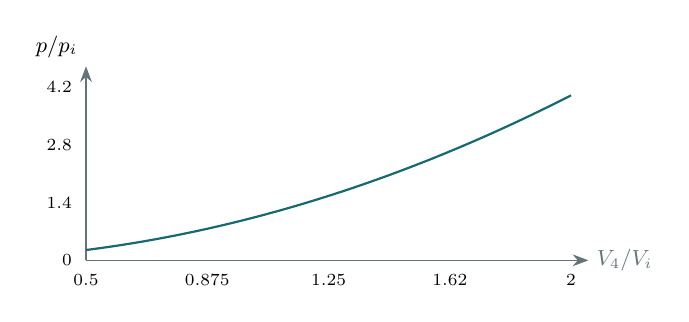
\begin{tikzpicture}[scale=.88,transform shape]
\draw[axis] (0,0.0000000)--(7.25,0.0000000) node[right] {$V_4/V_i$};
\draw[axis] (0.0000000,0)--(0.0000000,2.8);
\node[above left] at (0.0000000,2.8) {$p/p_i$};
\node[below,font=\scriptsize] at (0.0000000,-0.0800000) {$0.5$};
\node[below,font=\scriptsize] at (1.7500000,-0.0800000) {$0.875$};
\node[below,font=\scriptsize] at (3.5000000,-0.0800000) {$1.25$};
\node[below,font=\scriptsize] at (5.2500000,-0.0800000) {$1.62$};
\node[below,font=\scriptsize] at (7.0000000,-0.0800000) {$2$};
\node[left,font=\scriptsize] at (-0.0800000,0.0000000) {$0$};
\node[left,font=\scriptsize] at (-0.0800000,0.8333333) {$1.4$};
\node[left,font=\scriptsize] at (-0.0800000,1.6666667) {$2.8$};
\node[left,font=\scriptsize] at (-0.0800000,2.5000000) {$4.2$};
\draw[thick,color=accent] plot coordinates {(0.0000000,0.1488095) (0.0291667,0.1525530) (0.0583333,0.1563430) (0.0875000,0.1601795) (0.1166667,0.1640625) (0.1458333,0.1679920) (0.1750000,0.1719680) (0.2041667,0.1759905) (0.2333333,0.1800595) (0.2625000,0.1841750) (0.2916667,0.1883371) (0.3208333,0.1925456) (0.3500000,0.1968006) (0.3791667,0.2011021) (0.4083333,0.2054501) (0.4375000,0.2098447) (0.4666667,0.2142857) (0.4958333,0.2187733) (0.5250000,0.2233073) (0.5541667,0.2278878) (0.5833333,0.2325149) (0.6125000,0.2371884) (0.6416667,0.2419085) (0.6708333,0.2466750) (0.7000000,0.2514881) (0.7291667,0.2563477) (0.7583333,0.2612537) (0.7875000,0.2662063) (0.8166667,0.2712054) (0.8458333,0.2762509) (0.8750000,0.2813430) (0.9041667,0.2864816) (0.9333333,0.2916667) (0.9625000,0.2968983) (0.9916667,0.3021763) (1.0208333,0.3075009) (1.0500000,0.3128720) (1.0791667,0.3182896) (1.1083333,0.3237537) (1.1375000,0.3292643) (1.1666667,0.3348214) (1.1958333,0.3404250) (1.2250000,0.3460751) (1.2541667,0.3517718) (1.2833333,0.3575149) (1.3125000,0.3633045) (1.3416667,0.3691406) (1.3708333,0.3750233) (1.4000000,0.3809524) (1.4291667,0.3869280) (1.4583333,0.3929501) (1.4875000,0.3990188) (1.5166667,0.4051339) (1.5458333,0.4112956) (1.5750000,0.4175037) (1.6041667,0.4237584) (1.6333333,0.4300595) (1.6625000,0.4364072) (1.6916667,0.4428013) (1.7208333,0.4492420) (1.7500000,0.4557292) (1.7791667,0.4622628) (1.8083333,0.4688430) (1.8375000,0.4754697) (1.8666667,0.4821429) (1.8958333,0.4888625) (1.9250000,0.4956287) (1.9541667,0.5024414) (1.9833333,0.5093006) (2.0125000,0.5162063) (2.0416667,0.5231585) (2.0708333,0.5301572) (2.1000000,0.5372024) (2.1291667,0.5442941) (2.1583333,0.5514323) (2.1875000,0.5586170) (2.2166667,0.5658482) (2.2458333,0.5731259) (2.2750000,0.5804501) (2.3041667,0.5878209) (2.3333333,0.5952381) (2.3625000,0.6027018) (2.3916667,0.6102121) (2.4208333,0.6177688) (2.4500000,0.6253720) (2.4791667,0.6330218) (2.5083333,0.6407180) (2.5375000,0.6484608) (2.5666667,0.6562500) (2.5958333,0.6640858) (2.6250000,0.6719680) (2.6541667,0.6798968) (2.6833333,0.6878720) (2.7125000,0.6958938) (2.7416667,0.7039621) (2.7708333,0.7120768) (2.8000000,0.7202381) (2.8291667,0.7284459) (2.8583333,0.7367001) (2.8875000,0.7450009) (2.9166667,0.7533482) (2.9458333,0.7617420) (2.9750000,0.7701823) (3.0041667,0.7786691) (3.0333333,0.7872024) (3.0625000,0.7957822) (3.0916667,0.8044085) (3.1208333,0.8130813) (3.1500000,0.8218006) (3.1791667,0.8305664) (3.2083333,0.8393787) (3.2375000,0.8482375) (3.2666667,0.8571429) (3.2958333,0.8660947) (3.3250000,0.8750930) (3.3541667,0.8841378) (3.3833333,0.8932292) (3.4125000,0.9023670) (3.4416667,0.9115513) (3.4708333,0.9207822) (3.5000000,0.9300595) (3.5291667,0.9393834) (3.5583333,0.9487537) (3.5875000,0.9581706) (3.6166667,0.9676339) (3.6458333,0.9771438) (3.6750000,0.9867001) (3.7041667,0.9963030) (3.7333333,1.0059524) (3.7625000,1.0156483) (3.7916667,1.0253906) (3.8208333,1.0351795) (3.8500000,1.0450149) (3.8791667,1.0548968) (3.9083333,1.0648251) (3.9375000,1.0748000) (3.9666667,1.0848214) (3.9958333,1.0948893) (4.0250000,1.1050037) (4.0541667,1.1151646) (4.0833333,1.1253720) (4.1125000,1.1356259) (4.1416667,1.1459263) (4.1708333,1.1562733) (4.2000000,1.1666667) (4.2291667,1.1771066) (4.2583333,1.1875930) (4.2875000,1.1981259) (4.3166667,1.2087054) (4.3458333,1.2193313) (4.3750000,1.2300037) (4.4041667,1.2407227) (4.4333333,1.2514881) (4.4625000,1.2623000) (4.4916667,1.2731585) (4.5208333,1.2840634) (4.5500000,1.2950149) (4.5791667,1.3060128) (4.6083333,1.3170573) (4.6375000,1.3281483) (4.6666667,1.3392857) (4.6958333,1.3504697) (4.7250000,1.3617001) (4.7541667,1.3729771) (4.7833333,1.3843006) (4.8125000,1.3956706) (4.8416667,1.4070871) (4.8708333,1.4185500) (4.9000000,1.4300595) (4.9291667,1.4416155) (4.9583333,1.4532180) (4.9875000,1.4648670) (5.0166667,1.4765625) (5.0458333,1.4883045) (5.0750000,1.5000930) (5.1041667,1.5119280) (5.1333333,1.5238095) (5.1625000,1.5357375) (5.1916667,1.5477121) (5.2208333,1.5597331) (5.2500000,1.5718006) (5.2791667,1.5839146) (5.3083333,1.5960751) (5.3375000,1.6082822) (5.3666667,1.6205357) (5.3958333,1.6328358) (5.4250000,1.6451823) (5.4541667,1.6575753) (5.4833333,1.6700149) (5.5125000,1.6825009) (5.5416667,1.6950335) (5.5708333,1.7076125) (5.6000000,1.7202381) (5.6291667,1.7329102) (5.6583333,1.7456287) (5.6875000,1.7583938) (5.7166667,1.7712054) (5.7458333,1.7840634) (5.7750000,1.7969680) (5.8041667,1.8099191) (5.8333333,1.8229167) (5.8625000,1.8359608) (5.8916667,1.8490513) (5.9208333,1.8621884) (5.9500000,1.8753720) (5.9791667,1.8886021) (6.0083333,1.9018787) (6.0375000,1.9152018) (6.0666667,1.9285714) (6.0958333,1.9419875) (6.1250000,1.9554501) (6.1541667,1.9689593) (6.1833333,1.9825149) (6.2125000,1.9961170) (6.2416667,2.0097656) (6.2708333,2.0234608) (6.3000000,2.0372024) (6.3291667,2.0509905) (6.3583333,2.0648251) (6.3875000,2.0787063) (6.4166667,2.0926339) (6.4458333,2.1066081) (6.4750000,2.1206287) (6.5041667,2.1346959) (6.5333333,2.1488095) (6.5625000,2.1629697) (6.5916667,2.1771763) (6.6208333,2.1914295) (6.6500000,2.2057292) (6.6791667,2.2200753) (6.7083333,2.2344680) (6.7375000,2.2489072) (6.7666667,2.2633929) (6.7958333,2.2779250) (6.8250000,2.2925037) (6.8541667,2.3071289) (6.8833333,2.3218006) (6.9125000,2.3365188) (6.9416667,2.3512835) (6.9708333,2.3660947) (7.0000000,2.3809524)};
\end{tikzpicture}
\figcaption{变图综一.3V3\quad 压强正比体积平方的路径}
\end{minipage}\end{center}
变图综一.3V3显示$p/p_i=(V_4/V_i)^2$。一般指数$s$给$T\propto V_4^{s+1}$，故$C=2R+R/(s+1)$，$s\ne-1$。当$s=-1$时温度保持恒定，非零的体积功由吸热提供，采用等温过程的热量表达式。
\item \textbf{四倍体积的绝热膨胀。} 从$(V_i,T_i,p_i)$准静态绝热膨胀到$4V_i$，求末态和做功。
\par 主解给$TV_4^{1/2}$和$pV_4^{3/2}$分别保持不变，故
\[
T_f=\frac12T_i,\qquad p_f=\frac18p_i,\qquad
W=U_i-U_f=2\nu R(T_i-T_f)=\nu RT_i.
\]
\begin{center}\begin{minipage}{.98\linewidth}\centering
\begin{tikzpicture}[scale=.88,transform shape]
\draw[axis] (0,0.0000000)--(7.25,0.0000000) node[right] {$V_4/V_i$};
\draw[axis] (0.0000000,0)--(0.0000000,2.8);
\node[above left] at (0.0000000,2.8) {$\text{比值}$};
\node[below,font=\scriptsize] at (0.0000000,-0.0800000) {$1$};
\node[below,font=\scriptsize] at (1.7500000,-0.0800000) {$1.75$};
\node[below,font=\scriptsize] at (3.5000000,-0.0800000) {$2.5$};
\node[below,font=\scriptsize] at (5.2500000,-0.0800000) {$3.25$};
\node[below,font=\scriptsize] at (7.0000000,-0.0800000) {$4$};
\node[left,font=\scriptsize] at (-0.0800000,0.0000000) {$0$};
\node[left,font=\scriptsize] at (-0.0800000,0.8333333) {$0.35$};
\node[left,font=\scriptsize] at (-0.0800000,1.6666667) {$0.7$};
\node[left,font=\scriptsize] at (-0.0800000,2.5000000) {$1.05$};
\draw[thick,color=accent] plot coordinates {(0.0000000,2.3809524) (0.0291667,2.3662095) (0.0583333,2.3517371) (0.0875000,2.3375271) (0.1166667,2.3235716) (0.1458333,2.3098631) (0.1750000,2.2963944) (0.2041667,2.2831586) (0.2333333,2.2701490) (0.2625000,2.2573593) (0.2916667,2.2447834) (0.3208333,2.2324154) (0.3500000,2.2202495) (0.3791667,2.2082805) (0.4083333,2.1965029) (0.4375000,2.1849118) (0.4666667,2.1735022) (0.4958333,2.1622696) (0.5250000,2.1512093) (0.5541667,2.1403170) (0.5833333,2.1295885) (0.6125000,2.1190198) (0.6416667,2.1086069) (0.6708333,2.0983459) (0.7000000,2.0882334) (0.7291667,2.0782656) (0.7583333,2.0684393) (0.7875000,2.0587510) (0.8166667,2.0491975) (0.8458333,2.0397759) (0.8750000,2.0304830) (0.9041667,2.0213160) (0.9333333,2.0122720) (0.9625000,2.0033484) (0.9916667,1.9945424) (1.0208333,1.9858516) (1.0500000,1.9772733) (1.0791667,1.9688053) (1.1083333,1.9604452) (1.1375000,1.9521906) (1.1666667,1.9440395) (1.1958333,1.9359896) (1.2250000,1.9280389) (1.2541667,1.9201853) (1.2833333,1.9124270) (1.3125000,1.9047619) (1.3416667,1.8971883) (1.3708333,1.8897043) (1.4000000,1.8823081) (1.4291667,1.8749982) (1.4583333,1.8677727) (1.4875000,1.8606302) (1.5166667,1.8535689) (1.5458333,1.8465875) (1.5750000,1.8396843) (1.6041667,1.8328580) (1.6333333,1.8261071) (1.6625000,1.8194303) (1.6916667,1.8128262) (1.7208333,1.8062934) (1.7500000,1.7998308) (1.7791667,1.7934371) (1.8083333,1.7871110) (1.8375000,1.7808514) (1.8666667,1.7746571) (1.8958333,1.7685270) (1.9250000,1.7624600) (1.9541667,1.7564550) (1.9833333,1.7505110) (2.0125000,1.7446269) (2.0416667,1.7388018) (2.0708333,1.7330346) (2.1000000,1.7273244) (2.1291667,1.7216703) (2.1583333,1.7160714) (2.1875000,1.7105267) (2.2166667,1.7050354) (2.2458333,1.6995967) (2.2750000,1.6942097) (2.3041667,1.6888736) (2.3333333,1.6835876) (2.3625000,1.6783509) (2.3916667,1.6731628) (2.4208333,1.6680225) (2.4500000,1.6629293) (2.4791667,1.6578824) (2.5083333,1.6528813) (2.5375000,1.6479251) (2.5666667,1.6430132) (2.5958333,1.6381450) (2.6250000,1.6333199) (2.6541667,1.6285371) (2.6833333,1.6237960) (2.7125000,1.6190962) (2.7416667,1.6144369) (2.7708333,1.6098176) (2.8000000,1.6052378) (2.8291667,1.6006968) (2.8583333,1.5961941) (2.8875000,1.5917292) (2.9166667,1.5873016) (2.9458333,1.5829107) (2.9750000,1.5785561) (3.0041667,1.5742372) (3.0333333,1.5699535) (3.0625000,1.5657046) (3.0916667,1.5614901) (3.1208333,1.5573094) (3.1500000,1.5531621) (3.1791667,1.5490477) (3.2083333,1.5449659) (3.2375000,1.5409162) (3.2666667,1.5368982) (3.2958333,1.5329114) (3.3250000,1.5289555) (3.3541667,1.5250300) (3.3833333,1.5211347) (3.4125000,1.5172690) (3.4416667,1.5134327) (3.4708333,1.5096253) (3.5000000,1.5058465) (3.5291667,1.5020959) (3.5583333,1.4983733) (3.5875000,1.4946781) (3.6166667,1.4910102) (3.6458333,1.4873692) (3.6750000,1.4837546) (3.7041667,1.4801664) (3.7333333,1.4766040) (3.7625000,1.4730672) (3.7916667,1.4695557) (3.8208333,1.4660692) (3.8500000,1.4626074) (3.8791667,1.4591700) (3.9083333,1.4557568) (3.9375000,1.4523673) (3.9666667,1.4490015) (3.9958333,1.4456589) (4.0250000,1.4423394) (4.0541667,1.4390426) (4.0833333,1.4357683) (4.1125000,1.4325163) (4.1416667,1.4292863) (4.1708333,1.4260780) (4.2000000,1.4228912) (4.2291667,1.4197257) (4.2583333,1.4165812) (4.2875000,1.4134576) (4.3166667,1.4103545) (4.3458333,1.4072717) (4.3750000,1.4042091) (4.4041667,1.4011664) (4.4333333,1.3981434) (4.4625000,1.3951398) (4.4916667,1.3921556) (4.5208333,1.3891904) (4.5500000,1.3862441) (4.5791667,1.3833164) (4.6083333,1.3804072) (4.6375000,1.3775163) (4.6666667,1.3746435) (4.6958333,1.3717886) (4.7250000,1.3689514) (4.7541667,1.3661317) (4.7833333,1.3633294) (4.8125000,1.3605442) (4.8416667,1.3577761) (4.8708333,1.3550247) (4.9000000,1.3522901) (4.9291667,1.3495719) (4.9583333,1.3468701) (4.9875000,1.3441844) (5.0166667,1.3415147) (5.0458333,1.3388609) (5.0750000,1.3362227) (5.1041667,1.3336001) (5.1333333,1.3309928) (5.1625000,1.3284008) (5.1916667,1.3258239) (5.2208333,1.3232619) (5.2500000,1.3207148) (5.2791667,1.3181822) (5.3083333,1.3156642) (5.3375000,1.3131606) (5.3666667,1.3106711) (5.3958333,1.3081958) (5.4250000,1.3057345) (5.4541667,1.3032870) (5.4833333,1.3008532) (5.5125000,1.2984331) (5.5416667,1.2960263) (5.5708333,1.2936329) (5.6000000,1.2912527) (5.6291667,1.2888856) (5.6583333,1.2865315) (5.6875000,1.2841902) (5.7166667,1.2818617) (5.7458333,1.2795457) (5.7750000,1.2772423) (5.8041667,1.2749513) (5.8333333,1.2726726) (5.8625000,1.2704060) (5.8916667,1.2681515) (5.9208333,1.2659090) (5.9500000,1.2636783) (5.9791667,1.2614594) (6.0083333,1.2592521) (6.0375000,1.2570564) (6.0666667,1.2548721) (6.0958333,1.2526991) (6.1250000,1.2505375) (6.1541667,1.2483869) (6.1833333,1.2462474) (6.2125000,1.2441189) (6.2416667,1.2420013) (6.2708333,1.2398944) (6.3000000,1.2377982) (6.3291667,1.2357126) (6.3583333,1.2336375) (6.3875000,1.2315729) (6.4166667,1.2295185) (6.4458333,1.2274744) (6.4750000,1.2254405) (6.5041667,1.2234167) (6.5333333,1.2214028) (6.5625000,1.2193989) (6.5916667,1.2174047) (6.6208333,1.2154204) (6.6500000,1.2134457) (6.6791667,1.2114806) (6.7083333,1.2095250) (6.7375000,1.2075789) (6.7666667,1.2056421) (6.7958333,1.2037146) (6.8250000,1.2017963) (6.8541667,1.1998872) (6.8833333,1.1979872) (6.9125000,1.1960961) (6.9416667,1.1942140) (6.9708333,1.1923407) (7.0000000,1.1904762)};
\draw[thick,color=accent] (7.65,2.4)--(8.1,2.4);\node[right,font=\scriptsize] at (8.15,2.4) {$T/T_i$};
\draw[thick,dashed,color=warm] plot coordinates {(0.0000000,2.3809524) (0.0291667,2.3369970) (0.0583333,2.2943777) (0.0875000,2.2530382) (0.1166667,2.2129253) (0.1458333,2.1739888) (0.1750000,2.1361808) (0.2041667,2.0994562) (0.2333333,2.0637718) (0.2625000,2.0290871) (0.2916667,1.9953631) (0.3208333,1.9625630) (0.3500000,1.9306518) (0.3791667,1.8995961) (0.4083333,1.8693642) (0.4375000,1.8399257) (0.4666667,1.8112518) (0.4958333,1.7833151) (0.5250000,1.7560892) (0.5541667,1.7295491) (0.5833333,1.7036708) (0.6125000,1.6784315) (0.6416667,1.6538093) (0.6708333,1.6297833) (0.7000000,1.6063334) (0.7291667,1.5834405) (0.7583333,1.5610862) (0.7875000,1.5392531) (0.8166667,1.5179241) (0.8458333,1.4970832) (0.8750000,1.4767149) (0.9041667,1.4568043) (0.9333333,1.4373372) (0.9625000,1.4182997) (0.9916667,1.3996789) (1.0208333,1.3814620) (1.0500000,1.3636368) (1.0791667,1.3461917) (1.1083333,1.3291154) (1.1375000,1.3123971) (1.1666667,1.2960263) (1.1958333,1.2799931) (1.2250000,1.2642878) (1.2541667,1.2489010) (1.2833333,1.2338239) (1.3125000,1.2190476) (1.3416667,1.2045640) (1.3708333,1.1903649) (1.4000000,1.1764426) (1.4291667,1.1627896) (1.4583333,1.1493986) (1.4875000,1.1362627) (1.5166667,1.1233751) (1.5458333,1.1107293) (1.5750000,1.0983190) (1.6041667,1.0861381) (1.6333333,1.0741807) (1.6625000,1.0624410) (1.6916667,1.0509137) (1.7208333,1.0395933) (1.7500000,1.0284748) (1.7791667,1.0175530) (1.8083333,1.0068231) (1.8375000,0.9962805) (1.8666667,0.9859206) (1.8958333,0.9757391) (1.9250000,0.9657315) (1.9541667,0.9558939) (1.9833333,0.9462222) (2.0125000,0.9367124) (2.0416667,0.9273609) (2.0708333,0.9181640) (2.1000000,0.9091181) (2.1291667,0.9002198) (2.1583333,0.8914656) (2.1875000,0.8828525) (2.2166667,0.8743771) (2.2458333,0.8660365) (2.2750000,0.8578277) (2.3041667,0.8497477) (2.3333333,0.8417938) (2.3625000,0.8339632) (2.3916667,0.8262532) (2.4208333,0.8186613) (2.4500000,0.8111850) (2.4791667,0.8038218) (2.5083333,0.7965693) (2.5375000,0.7894252) (2.5666667,0.7823873) (2.5958333,0.7754533) (2.6250000,0.7686211) (2.6541667,0.7618887) (2.6833333,0.7552540) (2.7125000,0.7487150) (2.7416667,0.7422698) (2.7708333,0.7359166) (2.8000000,0.7296535) (2.8291667,0.7234788) (2.8583333,0.7173906) (2.8875000,0.7113874) (2.9166667,0.7054674) (2.9458333,0.6996290) (2.9750000,0.6938708) (3.0041667,0.6881911) (3.0333333,0.6825885) (3.0625000,0.6770615) (3.0916667,0.6716086) (3.1208333,0.6662286) (3.1500000,0.6609200) (3.1791667,0.6556816) (3.2083333,0.6505120) (3.2375000,0.6454099) (3.2666667,0.6403742) (3.2958333,0.6354037) (3.3250000,0.6304971) (3.3541667,0.6256533) (3.3833333,0.6208713) (3.4125000,0.6161499) (3.4416667,0.6114880) (3.4708333,0.6068845) (3.5000000,0.6023386) (3.5291667,0.5978491) (3.5583333,0.5934152) (3.5875000,0.5890357) (3.6166667,0.5847099) (3.6458333,0.5804367) (3.6750000,0.5762154) (3.7041667,0.5720450) (3.7333333,0.5679246) (3.7625000,0.5638535) (3.7916667,0.5598307) (3.8208333,0.5558556) (3.8500000,0.5519273) (3.8791667,0.5480451) (3.9083333,0.5442081) (3.9375000,0.5404158) (3.9666667,0.5366672) (3.9958333,0.5329618) (4.0250000,0.5292988) (4.0541667,0.5256777) (4.0833333,0.5220976) (4.1125000,0.5185579) (4.1416667,0.5150581) (4.1708333,0.5115975) (4.2000000,0.5081754) (4.2291667,0.5047914) (4.2583333,0.5014447) (4.2875000,0.4981348) (4.3166667,0.4948612) (4.3458333,0.4916233) (4.3750000,0.4884206) (4.4041667,0.4852524) (4.4333333,0.4821184) (4.4625000,0.4790180) (4.4916667,0.4759506) (4.5208333,0.4729159) (4.5500000,0.4699132) (4.5791667,0.4669422) (4.6083333,0.4640024) (4.6375000,0.4610933) (4.6666667,0.4582145) (4.6958333,0.4553655) (4.7250000,0.4525459) (4.7541667,0.4497553) (4.7833333,0.4469932) (4.8125000,0.4442593) (4.8416667,0.4415532) (4.8708333,0.4388744) (4.9000000,0.4362226) (4.9291667,0.4335974) (4.9583333,0.4309984) (4.9875000,0.4284253) (5.0166667,0.4258777) (5.0458333,0.4233552) (5.0750000,0.4208575) (5.1041667,0.4183843) (5.1333333,0.4159353) (5.1625000,0.4135100) (5.1916667,0.4111082) (5.2208333,0.4087296) (5.2500000,0.4063738) (5.2791667,0.4040405) (5.3083333,0.4017295) (5.3375000,0.3994405) (5.3666667,0.3971731) (5.3958333,0.3949270) (5.4250000,0.3927021) (5.4541667,0.3904980) (5.4833333,0.3883144) (5.5125000,0.3861511) (5.5416667,0.3840078) (5.5708333,0.3818843) (5.6000000,0.3797802) (5.6291667,0.3776954) (5.6583333,0.3756296) (5.6875000,0.3735826) (5.7166667,0.3715541) (5.7458333,0.3695439) (5.7750000,0.3675518) (5.8041667,0.3655774) (5.8333333,0.3636207) (5.8625000,0.3616814) (5.8916667,0.3597593) (5.9208333,0.3578541) (5.9500000,0.3559657) (5.9791667,0.3540939) (6.0083333,0.3522384) (6.0375000,0.3503990) (6.0666667,0.3485756) (6.0958333,0.3467679) (6.1250000,0.3449758) (6.1541667,0.3431992) (6.1833333,0.3414377) (6.2125000,0.3396912) (6.2416667,0.3379595) (6.2708333,0.3362425) (6.3000000,0.3345401) (6.3291667,0.3328519) (6.3583333,0.3311779) (6.3875000,0.3295178) (6.4166667,0.3278716) (6.4458333,0.3262391) (6.4750000,0.3246200) (6.5041667,0.3230143) (6.5333333,0.3214218) (6.5625000,0.3198423) (6.5916667,0.3182758) (6.6208333,0.3167219) (6.6500000,0.3151807) (6.6791667,0.3136519) (6.7083333,0.3121355) (6.7375000,0.3106312) (6.7666667,0.3091390) (6.7958333,0.3076587) (6.8250000,0.3061902) (6.8541667,0.3047333) (6.8833333,0.3032879) (6.9125000,0.3018539) (6.9416667,0.3004312) (6.9708333,0.2990196) (7.0000000,0.2976190)};
\draw[thick,dashed,color=warm] (7.65,1.9)--(8.1,1.9);\node[right,font=\scriptsize] at (8.15,1.9) {$p/p_i$};
\end{tikzpicture}
\figcaption{变图综一.3V4\quad 四倍体积绝热膨胀的温度和压强}
\end{minipage}\end{center}
变图综一.3V4沿同一过程画温度比和压强比。积分体积功也给$W=\int_{V_i}^{4V_i}p_i(V_i/V_4)^{3/2}\,\mathrm dV_4=p_iV_i=\nu RT_i$，内能减小量正好等于对外功。
\item \textbf{平动能分布。} 将四维速率密度换成单分子动能$\epsilon=mv^2/2$的概率密度，求最概然动能、平均动能和方差。
\par 取$y=\epsilon/(k_BT)=bv^2$，由$f_4(v)\,\mathrm dv=ye^{-y}\,\mathrm dy$，有
\[
g(\epsilon)=\frac{\epsilon}{(k_BT)^2}e^{-\epsilon/(k_BT)},\quad
\epsilon_{\rm mp}=k_BT,\quad\langle\epsilon\rangle=2k_BT,\quad
\operatorname{Var}\epsilon=2(k_BT)^2.
\]
\begin{center}\begin{minipage}{.98\linewidth}\centering
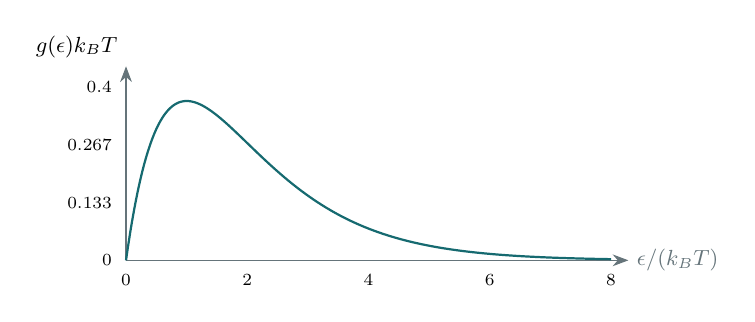
\begin{tikzpicture}[scale=.88,transform shape]
\draw[axis] (0,0.0000000)--(7.25,0.0000000) node[right] {$\epsilon/(k_BT)$};
\draw[axis] (0.0000000,0)--(0.0000000,2.8);
\node[above left] at (0.0000000,2.8) {$g(\epsilon)k_BT$};
\node[below,font=\scriptsize] at (0.0000000,-0.0800000) {$0$};
\node[below,font=\scriptsize] at (1.7500000,-0.0800000) {$2$};
\node[below,font=\scriptsize] at (3.5000000,-0.0800000) {$4$};
\node[below,font=\scriptsize] at (5.2500000,-0.0800000) {$6$};
\node[below,font=\scriptsize] at (7.0000000,-0.0800000) {$8$};
\node[left,font=\scriptsize] at (-0.0800000,0.0000000) {$0$};
\node[left,font=\scriptsize] at (-0.0800000,0.8333333) {$0.133$};
\node[left,font=\scriptsize] at (-0.0800000,1.6666667) {$0.267$};
\node[left,font=\scriptsize] at (-0.0800000,2.5000000) {$0.4$};
\draw[thick,color=accent] plot coordinates {(0.0000000,0.0000000) (0.0291667,0.2015034) (0.0583333,0.3897946) (0.0875000,0.5655234) (0.1166667,0.7293111) (0.1458333,0.8817518) (0.1750000,1.0234134) (0.2041667,1.1548390) (0.2333333,1.2765472) (0.2625000,1.3890342) (0.2916667,1.4927736) (0.3208333,1.5882181) (0.3500000,1.6758001) (0.3791667,1.7559326) (0.4083333,1.8290098) (0.4375000,1.8954083) (0.4666667,1.9554874) (0.4958333,2.0095901) (0.5250000,2.0580436) (0.5541667,2.1011603) (0.5833333,2.1392380) (0.6125000,2.1725607) (0.6416667,2.2013993) (0.6708333,2.2260120) (0.7000000,2.2466448) (0.7291667,2.2635323) (0.7583333,2.2768979) (0.7875000,2.2869543) (0.8166667,2.2939042) (0.8458333,2.2979404) (0.8750000,2.2992465) (0.9041667,2.2979972) (0.9333333,2.2943586) (0.9625000,2.2884887) (0.9916667,2.2805378) (1.0208333,2.2706485) (1.0500000,2.2589566) (1.0791667,2.2455908) (1.1083333,2.2306735) (1.1375000,2.2143208) (1.1666667,2.1966428) (1.1958333,2.1777440) (1.2250000,2.1577234) (1.2541667,2.1366750) (1.2833333,2.1146875) (1.3125000,2.0918453) (1.3416667,2.0682279) (1.3708333,2.0439108) (1.4000000,2.0189652) (1.4291667,1.9934585) (1.4583333,1.9674542) (1.4875000,1.9410124) (1.5166667,1.9141898) (1.5458333,1.8870397) (1.5750000,1.8596125) (1.6041667,1.8319554) (1.6333333,1.8041131) (1.6625000,1.7761274) (1.6916667,1.7480376) (1.7208333,1.7198806) (1.7500000,1.6916910) (1.7791667,1.6635013) (1.8083333,1.6353417) (1.8375000,1.6072406) (1.8666667,1.5792244) (1.8958333,1.5513177) (1.9250000,1.5235434) (1.9541667,1.4959229) (1.9833333,1.4684760) (2.0125000,1.4412209) (2.0416667,1.4141745) (2.0708333,1.3873526) (2.1000000,1.3607693) (2.1291667,1.3344379) (2.1583333,1.3083706) (2.1875000,1.2825781) (2.2166667,1.2570706) (2.2458333,1.2318571) (2.2750000,1.2069456) (2.3041667,1.1823436) (2.3333333,1.1580575) (2.3625000,1.1340930) (2.3916667,1.1104552) (2.4208333,1.0871483) (2.4500000,1.0641761) (2.4791667,1.0415417) (2.5083333,1.0192476) (2.5375000,0.9972959) (2.5666667,0.9756880) (2.5958333,0.9544250) (2.6250000,0.9335075) (2.6541667,0.9129358) (2.6833333,0.8927095) (2.7125000,0.8728283) (2.7416667,0.8532911) (2.7708333,0.8340969) (2.8000000,0.8152441) (2.8291667,0.7967309) (2.8583333,0.7785554) (2.8875000,0.7607153) (2.9166667,0.7432082) (2.9458333,0.7260314) (2.9750000,0.7091820) (3.0041667,0.6926571) (3.0333333,0.6764534) (3.0625000,0.6605678) (3.0916667,0.6449966) (3.1208333,0.6297365) (3.1500000,0.6147838) (3.1791667,0.6001346) (3.2083333,0.5857851) (3.2375000,0.5717315) (3.2666667,0.5579698) (3.2958333,0.5444960) (3.3250000,0.5313058) (3.3541667,0.5183953) (3.3833333,0.5057603) (3.4125000,0.4933966) (3.4416667,0.4812999) (3.4708333,0.4694661) (3.5000000,0.4578910) (3.5291667,0.4465702) (3.5583333,0.4354995) (3.5875000,0.4246748) (3.6166667,0.4140918) (3.6458333,0.4037462) (3.6750000,0.3936339) (3.7041667,0.3837507) (3.7333333,0.3740924) (3.7625000,0.3646550) (3.7916667,0.3554343) (3.8208333,0.3464263) (3.8500000,0.3376268) (3.8791667,0.3290320) (3.9083333,0.3206379) (3.9375000,0.3124405) (3.9666667,0.3044360) (3.9958333,0.2966205) (4.0250000,0.2889903) (4.0541667,0.2815415) (4.0833333,0.2742706) (4.1125000,0.2671738) (4.1416667,0.2602475) (4.1708333,0.2534882) (4.2000000,0.2468924) (4.2291667,0.2404566) (4.2583333,0.2341775) (4.2875000,0.2280516) (4.3166667,0.2220757) (4.3458333,0.2162465) (4.3750000,0.2105608) (4.4041667,0.2050156) (4.4333333,0.1996076) (4.4625000,0.1943338) (4.4916667,0.1891913) (4.5208333,0.1841771) (4.5500000,0.1792883) (4.5791667,0.1745222) (4.6083333,0.1698758) (4.6375000,0.1653465) (4.6666667,0.1609317) (4.6958333,0.1566285) (4.7250000,0.1524346) (4.7541667,0.1483473) (4.7833333,0.1443642) (4.8125000,0.1404828) (4.8416667,0.1367007) (4.8708333,0.1330156) (4.9000000,0.1294252) (4.9291667,0.1259273) (4.9583333,0.1225196) (4.9875000,0.1192000) (5.0166667,0.1159664) (5.0458333,0.1128167) (5.0750000,0.1097489) (5.1041667,0.1067609) (5.1333333,0.1038509) (5.1625000,0.1010170) (5.1916667,0.0982573) (5.2208333,0.0955700) (5.2500000,0.0929532) (5.2791667,0.0904053) (5.3083333,0.0879246) (5.3375000,0.0855093) (5.3666667,0.0831579) (5.3958333,0.0808688) (5.4250000,0.0786404) (5.4541667,0.0764712) (5.4833333,0.0743597) (5.5125000,0.0723045) (5.5416667,0.0703041) (5.5708333,0.0683571) (5.6000000,0.0664623) (5.6291667,0.0646182) (5.6583333,0.0628236) (5.6875000,0.0610772) (5.7166667,0.0593778) (5.7458333,0.0577242) (5.7750000,0.0561152) (5.8041667,0.0545496) (5.8333333,0.0530264) (5.8625000,0.0515444) (5.8916667,0.0501026) (5.9208333,0.0487000) (5.9500000,0.0473354) (5.9791667,0.0460080) (6.0083333,0.0447168) (6.0375000,0.0434607) (6.0666667,0.0422390) (6.0958333,0.0410507) (6.1250000,0.0398948) (6.1541667,0.0387707) (6.1833333,0.0376773) (6.2125000,0.0366140) (6.2416667,0.0355799) (6.2708333,0.0345743) (6.3000000,0.0335964) (6.3291667,0.0326454) (6.3583333,0.0317206) (6.3875000,0.0308215) (6.4166667,0.0299471) (6.4458333,0.0290970) (6.4750000,0.0282704) (6.5041667,0.0274668) (6.5333333,0.0266855) (6.5625000,0.0259258) (6.5916667,0.0251873) (6.6208333,0.0244694) (6.6500000,0.0237714) (6.6791667,0.0230930) (6.7083333,0.0224334) (6.7375000,0.0217923) (6.7666667,0.0211691) (6.7958333,0.0205634) (6.8250000,0.0199746) (6.8541667,0.0194023) (6.8833333,0.0188461) (6.9125000,0.0183055) (6.9416667,0.0177800) (6.9708333,0.0172694) (7.0000000,0.0167731)};
\end{tikzpicture}
\figcaption{变图综一.3V5\quad 四个二次自由度的动能密度}
\end{minipage}\end{center}
变图综一.3V5的密度在$y=1$取峰值。平均值和二阶矩分别由$\int_0^\infty y^2e^{-y}\mathrm dy=2!$、$\int_0^\infty y^3e^{-y}\mathrm dy=3!$求得。速率的最概然值对应动能$3k_BT/2$，能量密度的峰则为$k_BT$，变量变换的雅可比使两种密度的峰位置不同。
\item \textbf{超过指定速率的分子比例。} 求$v>v_*$的概率，并计算$v_*=v_{\rm rms}$时的比例。
\par 令$y_*=mv_*^2/(2k_BT)$，由动能分布积分，
\[
P(v>v_*)=\int_{y_*}^\infty ye^{-y}\,\mathrm dy=(1+y_*)e^{-y_*}.
\]
\begin{center}\begin{minipage}{.98\linewidth}\centering
\begin{tikzpicture}[scale=.88,transform shape]
\draw[axis] (0,0.0000000)--(7.25,0.0000000) node[right] {$v_*/\sqrt{k_BT/m}$};
\draw[axis] (0.0000000,0)--(0.0000000,2.8);
\node[above left] at (0.0000000,2.8) {$P(v>v_*)$};
\node[below,font=\scriptsize] at (0.0000000,-0.0800000) {$0$};
\node[below,font=\scriptsize] at (1.7500000,-0.0800000) {$1.25$};
\node[below,font=\scriptsize] at (3.5000000,-0.0800000) {$2.5$};
\node[below,font=\scriptsize] at (5.2500000,-0.0800000) {$3.75$};
\node[below,font=\scriptsize] at (7.0000000,-0.0800000) {$5$};
\node[left,font=\scriptsize] at (-0.0800000,0.0000000) {$0$};
\node[left,font=\scriptsize] at (-0.0800000,0.8333333) {$0.35$};
\node[left,font=\scriptsize] at (-0.0800000,1.6666667) {$0.7$};
\node[left,font=\scriptsize] at (-0.0800000,2.5000000) {$1.05$};
\draw[thick,color=accent] plot coordinates {(0.0000000,2.3809524) (0.0291667,2.3809523) (0.0583333,2.3809515) (0.0875000,2.3809478) (0.1166667,2.3809381) (0.1458333,2.3809175) (0.1750000,2.3808801) (0.2041667,2.3808187) (0.2333333,2.3807249) (0.2625000,2.3805888) (0.2916667,2.3803998) (0.3208333,2.3801458) (0.3500000,2.3798137) (0.3791667,2.3793897) (0.4083333,2.3788587) (0.4375000,2.3782048) (0.4666667,2.3774114) (0.4958333,2.3764610) (0.5250000,2.3753356) (0.5541667,2.3740165) (0.5833333,2.3724845) (0.6125000,2.3707200) (0.6416667,2.3687031) (0.6708333,2.3664136) (0.7000000,2.3638310) (0.7291667,2.3609349) (0.7583333,2.3577049) (0.7875000,2.3541205) (0.8166667,2.3501617) (0.8458333,2.3458084) (0.8750000,2.3410411) (0.9041667,2.3358405) (0.9333333,2.3301882) (0.9625000,2.3240660) (0.9916667,2.3174565) (1.0208333,2.3103432) (1.0500000,2.3027101) (1.0791667,2.2945423) (1.1083333,2.2858259) (1.1375000,2.2765477) (1.1666667,2.2666959) (1.1958333,2.2562595) (1.2250000,2.2452290) (1.2541667,2.2335959) (1.2833333,2.2213527) (1.3125000,2.2084937) (1.3416667,2.1950141) (1.3708333,2.1809105) (1.4000000,2.1661809) (1.4291667,2.1508247) (1.4583333,2.1348424) (1.4875000,2.1182362) (1.5166667,2.1010095) (1.5458333,2.0831669) (1.5750000,2.0647147) (1.6041667,2.0456602) (1.6333333,2.0260122) (1.6625000,2.0057807) (1.6916667,1.9849770) (1.7208333,1.9636135) (1.7500000,1.9417040) (1.7791667,1.9192632) (1.8083333,1.8963071) (1.8375000,1.8728526) (1.8666667,1.8489177) (1.8958333,1.8245213) (1.9250000,1.7996833) (1.9541667,1.7744242) (1.9833333,1.7487655) (2.0125000,1.7227294) (2.0416667,1.6963386) (2.0708333,1.6696164) (2.1000000,1.6425869) (2.1291667,1.6152743) (2.1583333,1.5877034) (2.1875000,1.5598994) (2.2166667,1.5318874) (2.2458333,1.5036931) (2.2750000,1.4753422) (2.3041667,1.4468603) (2.3333333,1.4182731) (2.3625000,1.3896065) (2.3916667,1.3608858) (2.4208333,1.3321366) (2.4500000,1.3033838) (2.4791667,1.2746524) (2.5083333,1.2459669) (2.5375000,1.2173513) (2.5666667,1.1888293) (2.5958333,1.1604242) (2.6250000,1.1321584) (2.6541667,1.1040540) (2.6833333,1.0761325) (2.7125000,1.0484147) (2.7416667,1.0209207) (2.7708333,0.9936697) (2.8000000,0.9666806) (2.8291667,0.9399711) (2.8583333,0.9135583) (2.8875000,0.8874585) (2.9166667,0.8616872) (2.9458333,0.8362590) (2.9750000,0.8111876) (3.0041667,0.7864859) (3.0333333,0.7621660) (3.0625000,0.7382392) (3.0916667,0.7147156) (3.1208333,0.6916049) (3.1500000,0.6689155) (3.1791667,0.6466553) (3.2083333,0.6248312) (3.2375000,0.6034492) (3.2666667,0.5825147) (3.2958333,0.5620322) (3.3250000,0.5420052) (3.3541667,0.5224367) (3.3833333,0.5033290) (3.4125000,0.4846834) (3.4416667,0.4665007) (3.4708333,0.4487809) (3.5000000,0.4315235) (3.5291667,0.4147271) (3.5583333,0.3983900) (3.5875000,0.3825096) (3.6166667,0.3670831) (3.6458333,0.3521069) (3.6750000,0.3375770) (3.7041667,0.3234888) (3.7333333,0.3098374) (3.7625000,0.2966176) (3.7916667,0.2838234) (3.8208333,0.2714488) (3.8500000,0.2594873) (3.8791667,0.2479322) (3.9083333,0.2367764) (3.9375000,0.2260126) (3.9666667,0.2156332) (3.9958333,0.2056305) (4.0250000,0.1959966) (4.0541667,0.1867233) (4.0833333,0.1778024) (4.1125000,0.1692256) (4.1416667,0.1609845) (4.1708333,0.1530704) (4.2000000,0.1454750) (4.2291667,0.1381894) (4.2583333,0.1312053) (4.2875000,0.1245138) (4.3166667,0.1181065) (4.3458333,0.1119748) (4.3750000,0.1061102) (4.4041667,0.1005042) (4.4333333,0.0951485) (4.4625000,0.0900347) (4.4916667,0.0851547) (4.5208333,0.0805005) (4.5500000,0.0760640) (4.5791667,0.0718374) (4.6083333,0.0678131) (4.6375000,0.0639834) (4.6666667,0.0603411) (4.6958333,0.0568788) (4.7250000,0.0535894) (4.7541667,0.0504660) (4.7833333,0.0475020) (4.8125000,0.0446906) (4.8416667,0.0420254) (4.8708333,0.0395003) (4.9000000,0.0371092) (4.9291667,0.0348462) (4.9583333,0.0327055) (4.9875000,0.0306818) (5.0166667,0.0287695) (5.0458333,0.0269635) (5.0750000,0.0252589) (5.1041667,0.0236507) (5.1333333,0.0221345) (5.1625000,0.0207055) (5.1916667,0.0193597) (5.2208333,0.0180927) (5.2500000,0.0169005) (5.2791667,0.0157795) (5.3083333,0.0147258) (5.3375000,0.0137360) (5.3666667,0.0128066) (5.3958333,0.0119345) (5.4250000,0.0111165) (5.4541667,0.0103496) (5.4833333,0.0096311) (5.5125000,0.0089583) (5.5416667,0.0083285) (5.5708333,0.0077394) (5.6000000,0.0071885) (5.6291667,0.0066737) (5.6583333,0.0061928) (5.6875000,0.0057439) (5.7166667,0.0053250) (5.7458333,0.0049344) (5.7750000,0.0045702) (5.8041667,0.0042309) (5.8333333,0.0039150) (5.8625000,0.0036210) (5.8916667,0.0033475) (5.9208333,0.0030932) (5.9500000,0.0028568) (5.9791667,0.0026373) (6.0083333,0.0024335) (6.0375000,0.0022444) (6.0666667,0.0020691) (6.0958333,0.0019065) (6.1250000,0.0017559) (6.1541667,0.0016165) (6.1833333,0.0014874) (6.2125000,0.0013680) (6.2416667,0.0012575) (6.2708333,0.0011555) (6.3000000,0.0010613) (6.3291667,0.0009742) (6.3583333,0.0008939) (6.3875000,0.0008199) (6.4166667,0.0007516) (6.4458333,0.0006887) (6.4750000,0.0006307) (6.5041667,0.0005774) (6.5333333,0.0005283) (6.5625000,0.0004832) (6.5916667,0.0004417) (6.6208333,0.0004036) (6.6500000,0.0003686) (6.6791667,0.0003365) (6.7083333,0.0003071) (6.7375000,0.0002801) (6.7666667,0.0002553) (6.7958333,0.0002327) (6.8250000,0.0002119) (6.8541667,0.0001929) (6.8833333,0.0001755) (6.9125000,0.0001596) (6.9416667,0.0001451) (6.9708333,0.0001319) (7.0000000,0.0001198)};
\end{tikzpicture}
\figcaption{变图综一.3V6\quad 四维速率分布的尾部概率}
\end{minipage}\end{center}
变图综一.3V6以$v_*/\sqrt{k_BT/m}$为横坐标画尾部比例。$v_*=v_{\rm rms}=2\sqrt{k_BT/m}$时$y_*=2$，所以比例为$3e^{-2}\simeq0.406$。方均根速率由平方平均确定，约四成分子的速率高于这个值。
\item \textbf{穿过小孔的分子速率。} 四维气体通过小孔作自由分子逸出，求逸出分子的速率密度、平均速率和最概然速率。
\par 各方向均匀，固定速率的向孔通量与$v$成正比，故归一化后的速率密度为$g(v)=vf_4(v)/\bar v$。因此
\[
\bar v_{\text{孔}}=\frac{\langle v^2\rangle}{\bar v}
=\frac{16}{3\sqrt{2\pi}}\sqrt{\frac{k_BT}{m}},\qquad
v_{{\rm mp},\text{孔}}=2\sqrt{\frac{k_BT}{m}}.
\]
\begin{center}\begin{minipage}{.98\linewidth}\centering
\begin{tikzpicture}[scale=.88,transform shape]
\draw[axis] (0,0.0000000)--(7.25,0.0000000) node[right] {$v/\sqrt{k_BT/m}$};
\draw[axis] (0.0000000,0)--(0.0000000,2.8);
\node[above left] at (0.0000000,2.8) {$\text{无量纲密度}$};
\node[below,font=\scriptsize] at (0.0000000,-0.0800000) {$0$};
\node[below,font=\scriptsize] at (1.7500000,-0.0800000) {$1.25$};
\node[below,font=\scriptsize] at (3.5000000,-0.0800000) {$2.5$};
\node[below,font=\scriptsize] at (5.2500000,-0.0800000) {$3.75$};
\node[below,font=\scriptsize] at (7.0000000,-0.0800000) {$5$};
\node[left,font=\scriptsize] at (-0.0800000,0.0000000) {$0$};
\node[left,font=\scriptsize] at (-0.0800000,0.8333333) {$0.233$};
\node[left,font=\scriptsize] at (-0.0800000,1.6666667) {$0.467$};
\node[left,font=\scriptsize] at (-0.0800000,2.5000000) {$0.7$};
\draw[thick,color=accent] plot coordinates {(0.0000000,0.0000000) (0.0291667,0.0000161) (0.0583333,0.0001291) (0.0875000,0.0004351) (0.1166667,0.0010298) (0.1458333,0.0020074) (0.1750000,0.0034606) (0.2041667,0.0054798) (0.2333333,0.0081532) (0.2625000,0.0115660) (0.2916667,0.0158002) (0.3208333,0.0209345) (0.3500000,0.0270433) (0.3791667,0.0341972) (0.4083333,0.0424619) (0.4375000,0.0518987) (0.4666667,0.0625635) (0.4958333,0.0745071) (0.5250000,0.0877747) (0.5541667,0.1024060) (0.5833333,0.1184347) (0.6125000,0.1358885) (0.6416667,0.1547891) (0.6708333,0.1751518) (0.7000000,0.1969859) (0.7291667,0.2202943) (0.7583333,0.2450737) (0.7875000,0.2713144) (0.8166667,0.2990005) (0.8458333,0.3281102) (0.8750000,0.3586154) (0.9041667,0.3904821) (0.9333333,0.4236706) (0.9625000,0.4581356) (0.9916667,0.4938265) (1.0208333,0.5306873) (1.0500000,0.5686571) (1.0791667,0.6076703) (1.1083333,0.6476570) (1.1375000,0.6885429) (1.1666667,0.7302500) (1.1958333,0.7726967) (1.2250000,0.8157983) (1.2541667,0.8594670) (1.2833333,0.9036126) (1.3125000,0.9481428) (1.3416667,0.9929631) (1.3708333,1.0379780) (1.4000000,1.0830905) (1.4291667,1.1282029) (1.4583333,1.1732172) (1.4875000,1.2180354) (1.5166667,1.2625596) (1.5458333,1.3066926) (1.5750000,1.3503382) (1.6041667,1.3934017) (1.6333333,1.4357897) (1.6625000,1.4774109) (1.6916667,1.5181762) (1.7208333,1.5579992) (1.7500000,1.5967960) (1.7791667,1.6344860) (1.8083333,1.6709916) (1.8375000,1.7062390) (1.8666667,1.7401578) (1.8958333,1.7726819) (1.9250000,1.8037488) (1.9541667,1.8333006) (1.9833333,1.8612836) (2.0125000,1.8876485) (2.0416667,1.9123505) (2.0708333,1.9353498) (2.1000000,1.9566109) (2.1291667,1.9761031) (2.1583333,1.9938006) (2.1875000,2.0096824) (2.2166667,2.0237319) (2.2458333,2.0359375) (2.2750000,2.0462921) (2.3041667,2.0547935) (2.3333333,2.0614435) (2.3625000,2.0662488) (2.3916667,2.0692202) (2.4208333,2.0703726) (2.4500000,2.0697252) (2.4791667,2.0673010) (2.5083333,2.0631267) (2.5375000,2.0572326) (2.5666667,2.0496527) (2.5958333,2.0404239) (2.6250000,2.0295863) (2.6541667,2.0171830) (2.6833333,2.0032596) (2.7125000,1.9878642) (2.7416667,1.9710474) (2.7708333,1.9528616) (2.8000000,1.9333612) (2.8291667,1.9126022) (2.8583333,1.8906421) (2.8875000,1.8675397) (2.9166667,1.8433547) (2.9458333,1.8181479) (2.9750000,1.7919804) (3.0041667,1.7649142) (3.0333333,1.7370112) (3.0625000,1.7083336) (3.0916667,1.6789434) (3.1208333,1.6489026) (3.1500000,1.6182724) (3.1791667,1.5871137) (3.2083333,1.5554867) (3.2375000,1.5234507) (3.2666667,1.4910638) (3.2958333,1.4583834) (3.3250000,1.4254653) (3.3541667,1.3923642) (3.3833333,1.3591332) (3.4125000,1.3258240) (3.4416667,1.2924866) (3.4708333,1.2591694) (3.5000000,1.2259189) (3.5291667,1.1927800) (3.5583333,1.1597957) (3.5875000,1.1270070) (3.6166667,1.0944529) (3.6458333,1.0621707) (3.6750000,1.0301956) (3.7041667,0.9985607) (3.7333333,0.9672974) (3.7625000,0.9364347) (3.7916667,0.9060001) (3.8208333,0.8760186) (3.8500000,0.8465138) (3.8791667,0.8175070) (3.9083333,0.7890177) (3.9375000,0.7610636) (3.9666667,0.7336606) (3.9958333,0.7068227) (4.0250000,0.6805623) (4.0541667,0.6548899) (4.0833333,0.6298148) (4.1125000,0.6053442) (4.1416667,0.5814842) (4.1708333,0.5582392) (4.2000000,0.5356123) (4.2291667,0.5136052) (4.2583333,0.4922184) (4.2875000,0.4714511) (4.3166667,0.4513014) (4.3458333,0.4317662) (4.3750000,0.4128417) (4.4041667,0.3945227) (4.4333333,0.3768033) (4.4625000,0.3596770) (4.4916667,0.3431361) (4.5208333,0.3271725) (4.5500000,0.3117772) (4.5791667,0.2969408) (4.6083333,0.2826533) (4.6375000,0.2689042) (4.6666667,0.2556825) (4.6958333,0.2429770) (4.7250000,0.2307759) (4.7541667,0.2190674) (4.7833333,0.2078392) (4.8125000,0.1970789) (4.8416667,0.1867740) (4.8708333,0.1769119) (4.9000000,0.1674798) (4.9291667,0.1584649) (4.9583333,0.1498545) (4.9875000,0.1416357) (5.0166667,0.1337959) (5.0458333,0.1263223) (5.0750000,0.1192025) (5.1041667,0.1124241) (5.1333333,0.1059747) (5.1625000,0.0998423) (5.1916667,0.0940149) (5.2208333,0.0884809) (5.2500000,0.0832286) (5.2791667,0.0782469) (5.3083333,0.0735248) (5.3375000,0.0690514) (5.3666667,0.0648162) (5.3958333,0.0608090) (5.4250000,0.0570198) (5.4541667,0.0534388) (5.4833333,0.0500568) (5.5125000,0.0468644) (5.5416667,0.0438529) (5.5708333,0.0410137) (5.6000000,0.0383386) (5.6291667,0.0358194) (5.6583333,0.0334486) (5.6875000,0.0312187) (5.7166667,0.0291224) (5.7458333,0.0271531) (5.7750000,0.0253039) (5.8041667,0.0235687) (5.8333333,0.0219412) (5.8625000,0.0204158) (5.8916667,0.0189867) (5.9208333,0.0176487) (5.9500000,0.0163967) (5.9791667,0.0152258) (6.0083333,0.0141314) (6.0375000,0.0131090) (6.0666667,0.0121545) (6.0958333,0.0112638) (6.1250000,0.0104331) (6.1541667,0.0096588) (6.1833333,0.0089375) (6.2125000,0.0082659) (6.2416667,0.0076410) (6.2708333,0.0070598) (6.3000000,0.0065196) (6.3291667,0.0060176) (6.3583333,0.0055516) (6.3875000,0.0051191) (6.4166667,0.0047180) (6.4458333,0.0043461) (6.4750000,0.0040016) (6.5041667,0.0036825) (6.5333333,0.0033873) (6.5625000,0.0031141) (6.5916667,0.0028616) (6.6208333,0.0026282) (6.6500000,0.0024127) (6.6791667,0.0022138) (6.7083333,0.0020303) (6.7375000,0.0018611) (6.7666667,0.0017051) (6.7958333,0.0015615) (6.8250000,0.0014292) (6.8541667,0.0013075) (6.8833333,0.0011956) (6.9125000,0.0010928) (6.9416667,0.0009982) (6.9708333,0.0009115) (7.0000000,0.0008318)};
\draw[thick,color=accent] (7.65,2.4)--(8.1,2.4);\node[right,font=\scriptsize] at (8.15,2.4) {$\text{气体内部}$};
\draw[thick,dashed,color=warm] plot coordinates {(0.0000000,0.0000000) (0.0291667,0.0000002) (0.0583333,0.0000029) (0.0875000,0.0000145) (0.1166667,0.0000456) (0.1458333,0.0001112) (0.1750000,0.0002301) (0.2041667,0.0004251) (0.2333333,0.0007228) (0.2625000,0.0011535) (0.2916667,0.0017509) (0.3208333,0.0025519) (0.3500000,0.0035962) (0.3791667,0.0049265) (0.4083333,0.0065877) (0.4375000,0.0086269) (0.4666667,0.0110930) (0.4958333,0.0140363) (0.5250000,0.0175085) (0.5541667,0.0215619) (0.5833333,0.0262492) (0.6125000,0.0316235) (0.6416667,0.0377373) (0.6708333,0.0446427) (0.7000000,0.0523907) (0.7291667,0.0610311) (0.7583333,0.0706119) (0.7875000,0.0811791) (0.8166667,0.0927764) (0.8458333,0.1054448) (0.8750000,0.1192224) (0.9041667,0.1341437) (0.9333333,0.1502401) (0.9625000,0.1675389) (0.9916667,0.1860634) (1.0208333,0.2058327) (1.0500000,0.2268613) (1.0791667,0.2491594) (1.1083333,0.2727321) (1.1375000,0.2975796) (1.1666667,0.3236973) (1.1958333,0.3510755) (1.2250000,0.3796992) (1.2541667,0.4095484) (1.2833333,0.4405980) (1.3125000,0.4728178) (1.3416667,0.5061725) (1.3708333,0.5406218) (1.4000000,0.5761208) (1.4291667,0.6126196) (1.4583333,0.6500638) (1.4875000,0.6883949) (1.5166667,0.7275499) (1.5458333,0.7674620) (1.5750000,0.8080605) (1.6041667,0.8492716) (1.6333333,0.8910179) (1.6625000,0.9332193) (1.6916667,0.9757931) (1.7208333,1.0186543) (1.7500000,1.0617158) (1.7791667,1.1048889) (1.8083333,1.1480836) (1.8375000,1.1912090) (1.8666667,1.2341734) (1.8958333,1.2768848) (1.9250000,1.3192514) (1.9541667,1.3611816) (1.9833333,1.4025845) (2.0125000,1.4433703) (2.0416667,1.4834507) (2.0708333,1.5227387) (2.1000000,1.5611496) (2.1291667,1.5986008) (2.1583333,1.6350123) (2.1875000,1.6703068) (2.2166667,1.7044102) (2.2458333,1.7372516) (2.2750000,1.7687636) (2.3041667,1.7988826) (2.3333333,1.8275488) (2.3625000,1.8547065) (2.3916667,1.8803042) (2.4208333,1.9042948) (2.4500000,1.9266354) (2.4791667,1.9472881) (2.5083333,1.9662191) (2.5375000,1.9833996) (2.5666667,1.9988054) (2.5958333,2.0124169) (2.6250000,2.0242195) (2.6541667,2.0342028) (2.6833333,2.0423615) (2.7125000,2.0486947) (2.7416667,2.0532058) (2.7708333,2.0559031) (2.8000000,2.0567987) (2.8291667,2.0559093) (2.8583333,2.0532554) (2.8875000,2.0488615) (2.9166667,2.0427559) (2.9458333,2.0349706) (2.9750000,2.0255408) (3.0041667,2.0145052) (3.0333333,2.0019053) (3.0625000,1.9877856) (3.0916667,1.9721934) (3.1208333,1.9551782) (3.1500000,1.9367918) (3.1791667,1.9170883) (3.2083333,1.8961232) (3.2375000,1.8739541) (3.2666667,1.8506395) (3.2958333,1.8262395) (3.3250000,1.8008149) (3.3541667,1.7744275) (3.3833333,1.7471395) (3.4125000,1.7190135) (3.4416667,1.6901125) (3.4708333,1.6604992) (3.5000000,1.6302363) (3.5291667,1.5993860) (3.5583333,1.5680102) (3.5875000,1.5361700) (3.6166667,1.5039255) (3.6458333,1.4713361) (3.6750000,1.4384600) (3.7041667,1.4053541) (3.7333333,1.3720740) (3.7625000,1.3386739) (3.7916667,1.3052062) (3.8208333,1.2717221) (3.8500000,1.2382705) (3.8791667,1.2048991) (3.9083333,1.1716533) (3.9375000,1.1385767) (3.9666667,1.1057111) (3.9958333,1.0730961) (4.0250000,1.0407694) (4.0541667,1.0087666) (4.0833333,0.9771212) (4.1125000,0.9458649) (4.1416667,0.9150269) (4.1708333,0.8846347) (4.2000000,0.8547136) (4.2291667,0.8252870) (4.2583333,0.7963762) (4.2875000,0.7680006) (4.3166667,0.7401776) (4.3458333,0.7129228) (4.3750000,0.6862500) (4.4041667,0.6601710) (4.4333333,0.6346962) (4.4625000,0.6098340) (4.4916667,0.5855914) (4.5208333,0.5619737) (4.5500000,0.5389848) (4.5791667,0.5166270) (4.6083333,0.4949015) (4.6375000,0.4738079) (4.6666667,0.4533448) (4.6958333,0.4335095) (4.7250000,0.4142982) (4.7541667,0.3957062) (4.7833333,0.3777276) (4.8125000,0.3603559) (4.8416667,0.3435833) (4.8708333,0.3274018) (4.9000000,0.3118023) (4.9291667,0.2967751) (4.9583333,0.2823100) (4.9875000,0.2683962) (5.0166667,0.2550226) (5.0458333,0.2421775) (5.0750000,0.2298489) (5.1041667,0.2180244) (5.1333333,0.2066914) (5.1625000,0.1958373) (5.1916667,0.1854489) (5.2208333,0.1755132) (5.2500000,0.1660171) (5.2791667,0.1569472) (5.3083333,0.1482903) (5.3375000,0.1400332) (5.3666667,0.1321627) (5.3958333,0.1246658) (5.4250000,0.1175293) (5.4541667,0.1107404) (5.4833333,0.1042865) (5.5125000,0.0981550) (5.5416667,0.0923336) (5.5708333,0.0868101) (5.6000000,0.0815727) (5.6291667,0.0766097) (5.6583333,0.0719097) (5.6875000,0.0674616) (5.7166667,0.0632545) (5.7458333,0.0592779) (5.7750000,0.0555214) (5.8041667,0.0519751) (5.8333333,0.0486293) (5.8625000,0.0454746) (5.8916667,0.0425019) (5.9208333,0.0397024) (5.9500000,0.0370676) (5.9791667,0.0345893) (6.0083333,0.0322596) (6.0375000,0.0300710) (6.0666667,0.0280160) (6.0958333,0.0260878) (6.1250000,0.0242795) (6.1541667,0.0225846) (6.1833333,0.0209971) (6.2125000,0.0195110) (6.2416667,0.0181206) (6.2708333,0.0168205) (6.3000000,0.0156056) (6.3291667,0.0144708) (6.3583333,0.0134117) (6.3875000,0.0124236) (6.4166667,0.0115023) (6.4458333,0.0106439) (6.4750000,0.0098445) (6.5041667,0.0091004) (6.5333333,0.0084082) (6.5625000,0.0077647) (6.5916667,0.0071667) (6.6208333,0.0066115) (6.6500000,0.0060961) (6.6791667,0.0056180) (6.7083333,0.0051748) (6.7375000,0.0047641) (6.7666667,0.0043838) (6.7958333,0.0040317) (6.8250000,0.0037061) (6.8541667,0.0034051) (6.8833333,0.0031269) (6.9125000,0.0028700) (6.9416667,0.0026328) (6.9708333,0.0024141) (7.0000000,0.0022124)};
\draw[thick,dashed,color=warm] (7.65,1.9)--(8.1,1.9);\node[right,font=\scriptsize] at (8.15,1.9) {$\text{穿孔分子}$};
\end{tikzpicture}
\figcaption{变图综一.3V7\quad 穿孔通量对速率增加一个权重}
\end{minipage}\end{center}
变图综一.3V7画气体内部与穿孔分子的归一化速率密度。穿孔密度多一个$v$因子，快速分子在同样时间内到达小孔的机会更多，平均速率约为$2.128\sqrt{k_BT/m}$，高于气体内部的$1.880\sqrt{k_BT/m}$。
\item \textbf{升压直线路径的熵变。} 四维理想气体沿$p=aV_4$从$V_i$膨胀到$2V_i$，求温度、热量、功和熵变。
\par 状态方程给$T_f=4T_i$，而$C=5R/2$，故$Q=(5/2)\nu R(3T_i)=15\nu RT_i/2$。体积功为$W=\int_{V_i}^{2V_i}aV_4\,\mathrm dV_4=3\nu RT_i/2$，内能增量为$6\nu RT_i$。熵变为
\[
\Delta S=\nu C_V\ln\frac{T_f}{T_i}+\nu R\ln\frac{V_f}{V_i}
=5\nu R\ln2.
\]
\begin{center}\begin{minipage}{.98\linewidth}\centering
\begin{tikzpicture}[scale=.88,transform shape]
\draw[axis] (0,0.0000000)--(7.25,0.0000000) node[right] {$V_4/V_i$};
\draw[axis] (0.0000000,0)--(0.0000000,2.8);
\node[above left] at (0.0000000,2.8) {$\Delta S/(\nu R)$};
\node[below,font=\scriptsize] at (0.0000000,-0.0800000) {$1$};
\node[below,font=\scriptsize] at (1.7500000,-0.0800000) {$1.25$};
\node[below,font=\scriptsize] at (3.5000000,-0.0800000) {$1.5$};
\node[below,font=\scriptsize] at (5.2500000,-0.0800000) {$1.75$};
\node[below,font=\scriptsize] at (7.0000000,-0.0800000) {$2$};
\node[left,font=\scriptsize] at (-0.0800000,0.0000000) {$0$};
\node[left,font=\scriptsize] at (-0.0800000,0.8333333) {$1.2$};
\node[left,font=\scriptsize] at (-0.0800000,1.6666667) {$2.4$};
\node[left,font=\scriptsize] at (-0.0800000,2.5000000) {$3.6$};
\draw[thick,color=accent] plot coordinates {(0.0000000,0.0000000) (0.0291667,0.0144375) (0.0583333,0.0288153) (0.0875000,0.0431337) (0.1166667,0.0573934) (0.1458333,0.0715947) (0.1750000,0.0857382) (0.2041667,0.0998244) (0.2333333,0.1138536) (0.2625000,0.1278263) (0.2916667,0.1417430) (0.3208333,0.1556042) (0.3500000,0.1694103) (0.3791667,0.1831617) (0.4083333,0.1968588) (0.4375000,0.2105022) (0.4666667,0.2240921) (0.4958333,0.2376290) (0.5250000,0.2511134) (0.5541667,0.2645456) (0.5833333,0.2779261) (0.6125000,0.2912552) (0.6416667,0.3045333) (0.6708333,0.3177608) (0.7000000,0.3309381) (0.7291667,0.3440656) (0.7583333,0.3571437) (0.7875000,0.3701727) (0.8166667,0.3831530) (0.8458333,0.3960849) (0.8750000,0.4089689) (0.9041667,0.4218052) (0.9333333,0.4345942) (0.9625000,0.4473364) (0.9916667,0.4600319) (1.0208333,0.4726812) (1.0500000,0.4852845) (1.0791667,0.4978423) (1.1083333,0.5103548) (1.1375000,0.5228224) (1.1666667,0.5352454) (1.1958333,0.5476241) (1.2250000,0.5599588) (1.2541667,0.5722499) (1.2833333,0.5844976) (1.3125000,0.5967023) (1.3416667,0.6088642) (1.3708333,0.6209837) (1.4000000,0.6330610) (1.4291667,0.6450964) (1.4583333,0.6570903) (1.4875000,0.6690429) (1.5166667,0.6809544) (1.5458333,0.6928253) (1.5750000,0.7046557) (1.6041667,0.7164459) (1.6333333,0.7281963) (1.6625000,0.7399070) (1.6916667,0.7515783) (1.7208333,0.7632106) (1.7500000,0.7748040) (1.7791667,0.7863588) (1.8083333,0.7978753) (1.8375000,0.8093538) (1.8666667,0.8207944) (1.8958333,0.8321974) (1.9250000,0.8435631) (1.9541667,0.8548918) (1.9833333,0.8661835) (2.0125000,0.8774387) (2.0416667,0.8886575) (2.0708333,0.8998402) (2.1000000,0.9109870) (2.1291667,0.9220981) (2.1583333,0.9331738) (2.1875000,0.9442143) (2.2166667,0.9552198) (2.2458333,0.9661905) (2.2750000,0.9771266) (2.3041667,0.9880284) (2.3333333,0.9988961) (2.3625000,1.0097299) (2.3916667,1.0205299) (2.4208333,1.0312965) (2.4500000,1.0420298) (2.4791667,1.0527301) (2.5083333,1.0633974) (2.5375000,1.0740321) (2.5666667,1.0846343) (2.5958333,1.0952043) (2.6250000,1.1057421) (2.6541667,1.1162481) (2.6833333,1.1267224) (2.7125000,1.1371652) (2.7416667,1.1475766) (2.7708333,1.1579570) (2.8000000,1.1683064) (2.8291667,1.1786250) (2.8583333,1.1889131) (2.8875000,1.1991708) (2.9166667,1.2093982) (2.9458333,1.2195957) (2.9750000,1.2297632) (3.0041667,1.2399011) (3.0333333,1.2500095) (3.0625000,1.2600885) (3.0916667,1.2701384) (3.1208333,1.2801592) (3.1500000,1.2901512) (3.1791667,1.3001146) (3.2083333,1.3100494) (3.2375000,1.3199559) (3.2666667,1.3298342) (3.2958333,1.3396845) (3.3250000,1.3495069) (3.3541667,1.3593016) (3.3833333,1.3690688) (3.4125000,1.3788085) (3.4416667,1.3885211) (3.4708333,1.3982065) (3.5000000,1.4078650) (3.5291667,1.4174966) (3.5583333,1.4271017) (3.5875000,1.4366802) (3.6166667,1.4462324) (3.6458333,1.4557584) (3.6750000,1.4652584) (3.7041667,1.4747324) (3.7333333,1.4841806) (3.7625000,1.4936032) (3.7916667,1.5030003) (3.8208333,1.5123720) (3.8500000,1.5217185) (3.8791667,1.5310399) (3.9083333,1.5403364) (3.9375000,1.5496080) (3.9666667,1.5588549) (3.9958333,1.5680773) (4.0250000,1.5772753) (4.0541667,1.5864489) (4.0833333,1.5955984) (4.1125000,1.6047238) (4.1416667,1.6138253) (4.1708333,1.6229030) (4.2000000,1.6319570) (4.2291667,1.6409875) (4.2583333,1.6499946) (4.2875000,1.6589784) (4.3166667,1.6679389) (4.3458333,1.6768765) (4.3750000,1.6857910) (4.4041667,1.6946828) (4.4333333,1.7035518) (4.4625000,1.7123982) (4.4916667,1.7212222) (4.5208333,1.7300238) (4.5500000,1.7388031) (4.5791667,1.7475603) (4.6083333,1.7562954) (4.6375000,1.7650087) (4.6666667,1.7737001) (4.6958333,1.7823698) (4.7250000,1.7910179) (4.7541667,1.7996446) (4.7833333,1.8082498) (4.8125000,1.8168338) (4.8416667,1.8253967) (4.8708333,1.8339384) (4.9000000,1.8424592) (4.9291667,1.8509591) (4.9583333,1.8594383) (4.9875000,1.8678968) (5.0166667,1.8763348) (5.0458333,1.8847523) (5.0750000,1.8931495) (5.1041667,1.9015264) (5.1333333,1.9098831) (5.1625000,1.9182198) (5.1916667,1.9265365) (5.2208333,1.9348333) (5.2500000,1.9431104) (5.2791667,1.9513677) (5.3083333,1.9596055) (5.3375000,1.9678238) (5.3666667,1.9760227) (5.3958333,1.9842022) (5.4250000,1.9923626) (5.4541667,2.0005038) (5.4833333,2.0086259) (5.5125000,2.0167292) (5.5416667,2.0248135) (5.5708333,2.0328791) (5.6000000,2.0409259) (5.6291667,2.0489542) (5.6583333,2.0569639) (5.6875000,2.0649552) (5.7166667,2.0729282) (5.7458333,2.0808829) (5.7750000,2.0888194) (5.8041667,2.0967378) (5.8333333,2.1046382) (5.8625000,2.1125207) (5.8916667,2.1203853) (5.9208333,2.1282321) (5.9500000,2.1360612) (5.9791667,2.1438728) (6.0083333,2.1516668) (6.0375000,2.1594433) (6.0666667,2.1672025) (6.0958333,2.1749443) (6.1250000,2.1826690) (6.1541667,2.1903764) (6.1833333,2.1980669) (6.2125000,2.2057403) (6.2416667,2.2133968) (6.2708333,2.2210364) (6.3000000,2.2286593) (6.3291667,2.2362655) (6.3583333,2.2438551) (6.3875000,2.2514281) (6.4166667,2.2589846) (6.4458333,2.2665247) (6.4750000,2.2740485) (6.5041667,2.2815560) (6.5333333,2.2890473) (6.5625000,2.2965225) (6.5916667,2.3039816) (6.6208333,2.3114248) (6.6500000,2.3188520) (6.6791667,2.3262634) (6.7083333,2.3336589) (6.7375000,2.3410388) (6.7666667,2.3484030) (6.7958333,2.3557516) (6.8250000,2.3630847) (6.8541667,2.3704024) (6.8833333,2.3777046) (6.9125000,2.3849916) (6.9416667,2.3922632) (6.9708333,2.3995197) (7.0000000,2.4067610)};
\end{tikzpicture}
\figcaption{变图综一.3V8\quad 升压直线路径中的熵增}
\end{minipage}\end{center}
变图综一.3V8画该路径的$\Delta S/(\nu R)=5\ln(V_4/V_i)$。沿可逆路径积分$\int\delta Q/T=(5/2)\nu R\ln4$得到相同结果，温度变化和体积变化都对熵的增加作出贡献。
\end{enumerate}

\Needspace{13\baselineskip}

\pdfbookmark[2]{第 4 题 三个频率电源的稳态电流与平均功率}{q4}

\section*{第 4 题\quad 三个频率电源的稳态电流与平均功率}\label{q:4}


理想电压源、电阻、电感和电容按图连接。底部导线为参考电势零；左电源$\mathcal E_1$使左侧电阻端电势升为$\mathcal E_1$，中、右两电源$\mathcal E_2,\mathcal E_3$的电势升高方向均向下。电阻电流$i$正方向向上经过左支路，再由左向右流过电阻。
\[
\begin{aligned}
\mathcal E_1&=E_0\cos(\tfrac12\omega t+30^\circ),\\
\mathcal E_2&=E_0\cos(\omega t+45^\circ),\\
\mathcal E_3&=E_0\cos(2\omega t+60^\circ).
\end{aligned}
\]
已知$\omega L=1/(\omega C)=R$。求电阻的稳态电流$i(t)$，并求长时间平均消耗功率。须写出逐频率叠加和时间平均的依据。


\begin{center}\begin{minipage}{.98\linewidth}\centering
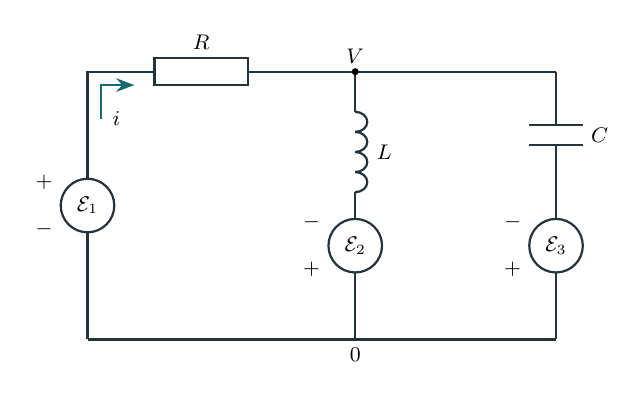
\begin{tikzpicture}[scale=.85,transform shape]

\draw[object] (0,0)--(0,1.6); \draw[object] (0,2.4)--(0,4)--(1,4);
\draw[object] (1,3.8) rectangle (2.4,4.2); \node[above] at (1.7,4.2) {$R$};
\draw[object] (2.4,4)--(7,4);
\draw[object] (0,0)--(7,0);
\draw[object] (0,2) circle (.4); \node at (0,2) {$\mathcal E_1$};
\node[left] at (-.4,2.35) {$+$};\node[left] at (-.4,1.65) {$-$};
\draw[object] (4,4)--(4,3.4);
\foreach \y in {3.4,3.1,2.8,2.5}{\draw[object] (4,\y) arc[start angle=90,end angle=-90,x radius=.18,y radius=.15];}
\node[right] at (4.2,2.8) {$L$};
\draw[object] (4,2.2)--(4,1.8); \draw[object] (4,1.4) circle (.4);
\draw[object] (4,1)--(4,0);
\node at (4,1.4) {$\mathcal E_2$};
\node[left] at (3.6,1.75) {$-$};\node[left] at (3.6,1.05) {$+$};
\draw[object] (7,4)--(7,3.2); \draw[object] (6.6,3.2)--(7.4,3.2);
\draw[object] (6.6,2.9)--(7.4,2.9); \draw[object] (7,2.9)--(7,1.8);
\node[right] at (7.4,3.05) {$C$};
\draw[object] (7,1.4) circle (.4); \node at (7,1.4) {$\mathcal E_3$};
\draw[object] (7,1)--(7,0);
\node[left] at (6.6,1.75) {$-$};\node[left] at (6.6,1.05) {$+$};
\draw[motion] (.2,3.3)--(.2,3.8)--(.7,3.8);
\node[right] at (.25,3.3) {$i$};
\fill (4,4) circle (1.5pt) node[above] {$V$};
\node[below] at (4,0) {$0$};

\end{tikzpicture}
\figcaption{图综一.4\quad 电源极性与电阻电流方向；三电源的频率依次为$\omega/2$、$\omega$、$2\omega$。}
\end{minipage}\end{center}

\Needspace{8\baselineskip}

\pdfbookmark[3]{题型定位}{q4-h0}

\subsection*{题型定位}

线性电路的多频率稳态分析。三个独立单频问题各有不同电抗，按图中电源升压方向和电阻参考电流逐支路列式，再把时间函数相加。

\Needspace{8\baselineskip}

\pdfbookmark[3]{知识点}{q4-h1}

\subsection*{知识点}

\begin{itemize}
\item 电压源置零短路、叠加定理与单频相量。
\item 电感电容频率依赖、串并联阻抗和分流。
\item 内部支路电源对节点的驱动，以及电感、电容导纳相消时的返回电流。
\item 峰值和有效值、共同周期正交积分及平均焦耳功率。
\end{itemize}

\Needspace{8\baselineskip}

\pdfbookmark[3]{物理图像}{q4-h2}

\subsection*{物理图像}

解图综一.4A、B、C逐个短接另外两个电源，保留相应阻抗数值和返回电阻的方向。D用$\omega$/2、$\omega$、2$\omega$三条谱线表示三个独立幅值，图A、B、C中的相量各以本频率旋转；图D把它们放在不同谱线上，平均发热由谱线高度平方分别求出后相加。

\Needspace{8\baselineskip}

\pdfbookmark[3]{解题入口}{q4-h3}

\subsection*{解题入口}

先按图综一.4的电源极性写上节点方程，固定中、右支路向下及电阻向上的电流。随后按图A、B、C分别写出$Z_L$、$Z_C$，用串并联阻抗求电源支路电流，再按导纳分流得到电阻返回电流。中频把节点方程中的$E_2/Z_L$保留到最后。三个时域表达式相加后，以$4\pi/\omega$为积分区间计算功率。

\Needspace{8\baselineskip}

\pdfbookmark[3]{标准解法}{q4-h4}

\subsection*{标准解法}


图综一.4中三个电源频率依次为$\omega/2$、$\omega$和$2\omega$。电路中的电阻、电感和电容均满足线性关系，电流可逐频率求出后在时域相加。保留一个电源时，其余理想电压源置零为短路，图中的上下节点及支路连接保持相同。以下相量的模取正弦量的峰值，记虚数单位为$\mathrm j$。

先用图中上节点$V$统一支路方向：设上节点电势相量为$V$，对应频率的电源相量为$E_1,E_2,E_3$，各不在本频率的电源置零。依图上极性，
\[
I=\frac{E_1-V}{R}
=\frac{V+E_2}{Z_L}+\frac{V+E_3}{Z_C}.
\]
中、右支路均取向下电流为正，$Z_L=\mathrm j\Omega L$、$Z_C=1/(\mathrm j\Omega C)$，每算一个频率都应重新代入$\Omega$。
\begin{center}\begin{minipage}{.98\linewidth}\centering
\begin{tikzpicture}[scale=.85,transform shape]

\node at (3.4,5.3) {$\Omega=\omega/2$，仅$\mathcal E_1$工作};
\draw[object] (0,0)--(0,4)--(1,4);
\draw[object] (1,3.8) rectangle (2.4,4.2); \node[above] at (1.7,4.2) {$R$};
\draw[object] (2.4,4)--(7,4); \draw[object] (0,0)--(7,0);
\draw[object] (4,4)--(4,3.4); \draw[object] (3.7,2.4) rectangle (4.3,3.4);
\node[right] at (4.3,2.9) {$ \mathrm jR/2 $};
\draw[object] (4,2.4)--(4,0);
\draw[object] (7,4)--(7,3.4); \draw[object] (6.7,2.4) rectangle (7.3,3.4);
\node[right] at (7.3,2.9) {$ -2\mathrm jR $}; \draw[object] (7,2.4)--(7,0);
\draw[motion] (0,3.3)--(0,3.7)--(.6,3.7); \node[left] at (0,3.3) {$I_1$};
\fill[white] (-0.09,.8) rectangle (0.09,1.8);\draw[object] (0,1.3) circle (.5);\node at (0,1.3) {$E_1$};\node[left] at (-0.5,1.7) {$+$};\node[left] at (-0.5,.9) {$-$};
\end{tikzpicture}
\figcaption{解图综一.4A\quad 低频分量：电阻串联LC并联阻抗。}
\end{minipage}\end{center}
三个电源分别激励的回路虽有不同的串并联组合，其节点式可统一整理为
\[
D=\frac1R+\frac1{Z_L}+\frac1{Z_C},\qquad
V=\frac{E_1/R-E_2/Z_L-E_3/Z_C}{D}.
\]
例如低频时$D=(1-3\mathrm j/2)/R$，节点电压等于$E_1/(1-3\mathrm j/2)$，代入$I_1=(E_1-V)/R$便得到图A的电流。高频时$D=(1+3\mathrm j/2)/R$，节点电压由右支路的$-E_3/Z_C$项决定，电阻电流向上返回为$-V/R$。这两个方向与图A、C的箭头相同。

解图综一.4A对应$\Omega=\omega/2$，仅保留$\mathcal E_1$。此时
\[
Z_L=\frac{\mathrm jR}{2},\qquad Z_C=-2\mathrm jR,
\qquad
Z_{LC}=\frac{Z_LZ_C}{Z_L+Z_C}=\frac{2\mathrm jR}{3}.
\]
电源看到$R+Z_{LC}=R(1+2\mathrm j/3)$，电阻电流为
\[
I_1=\frac{E_0e^{\mathrm j30^\circ}}{R(1+2\mathrm j/3)}
=\frac{3E_0}{\sqrt{13}R}
e^{\mathrm j[30^\circ-\arctan(2/3)]}.
\]
所以
\[
i_1(t)=\frac{3E_0}{\sqrt{13}R}
\cos\left(\frac{\omega t}{2}+30^\circ-\arctan\frac23\right).
\]
该分量电流滞后自身电源$\arctan(2/3)$，相位约$-3.69^\circ$。
\begin{center}\begin{minipage}{.98\linewidth}\centering
\begin{tikzpicture}[scale=.85,transform shape]

\node at (3.4,5.3) {$\Omega=\omega$，仅$\mathcal E_2$工作};
\draw[object] (0,0)--(0,4)--(1,4);
\draw[object] (1,3.8) rectangle (2.4,4.2); \node[above] at (1.7,4.2) {$R$};
\draw[object] (2.4,4)--(7,4); \draw[object] (0,0)--(7,0);
\draw[object] (4,4)--(4,3.4); \draw[object] (3.7,2.4) rectangle (4.3,3.4);
\node[right] at (4.3,2.9) {$ \mathrm jR $};
\draw[object] (4,2.4)--(4,0);
\draw[object] (7,4)--(7,3.4); \draw[object] (6.7,2.4) rectangle (7.3,3.4);
\node[right] at (7.3,2.9) {$ -\mathrm jR $}; \draw[object] (7,2.4)--(7,0);
\draw[motion] (0,3.3)--(0,3.7)--(.6,3.7); \node[left] at (0,3.3) {$I_2$};
\fill[white] (3.91,.8) rectangle (4.09,1.8);\draw[object] (4,1.3) circle (.5);\node at (4,1.3) {$E_2$};\node[left] at (3.5,1.7) {$-$};\node[left] at (3.5,.9) {$+$};
\end{tikzpicture}
\figcaption{解图综一.4B\quad 中频分量：内部电源通过电感及R、C并联返回，电阻电流非零。}
\end{minipage}\end{center}
解图综一.4B对应$\Omega=\omega$，仅保留$\mathcal E_2$。电感与中间电源串联，外部回路由$R$和$C$并联构成。沿中间电源升压方向取向下电流$J_2$，
\[
Z_{R\parallel C}=\frac{R(-\mathrm jR)}{R-\mathrm jR}
=\frac R2(1-\mathrm j),\qquad
Z_{\rm total}=\frac R2(1+\mathrm j).
\]
于是
\[
J_2=\frac{E_0e^{\mathrm j45^\circ}}{(R/2)(1+\mathrm j)}
=\frac{\sqrt2 E_0}{R}.
\]
并联部分向上返回的电阻电流按导纳分流：
\[
I_2=J_2\frac{Z_C}{R+Z_C}
=J_2\frac{1-\mathrm j}{2}
=\frac{E_0}{R}e^{-\mathrm j45^\circ}.
\]
因此
\[
i_2(t)=\frac{E_0}{R}\cos(\omega t-45^\circ).
\]
在$\Omega=\omega$时，$1/Z_L+1/Z_C=0$，节点方程化为$-V/R=E_2/Z_L$。图B的中间电源与电感串联，$E_2/Z_L$驱动电流沿电感支路向下，再由左侧电阻向上返回。于是$V=\mathrm jE_2$，$I_2=-V/R=-\mathrm jE_2/R$，与分流步骤给出的相位一致。
\begin{center}\begin{minipage}{.98\linewidth}\centering
\begin{tikzpicture}[scale=.85,transform shape]

\node at (3.4,5.3) {$\Omega=2\omega$，仅$\mathcal E_3$工作};
\draw[object] (0,0)--(0,4)--(1,4);
\draw[object] (1,3.8) rectangle (2.4,4.2); \node[above] at (1.7,4.2) {$R$};
\draw[object] (2.4,4)--(7,4); \draw[object] (0,0)--(7,0);
\draw[object] (4,4)--(4,3.4); \draw[object] (3.7,2.4) rectangle (4.3,3.4);
\node[right] at (4.3,2.9) {$ 2\mathrm jR $};
\draw[object] (4,2.4)--(4,0);
\draw[object] (7,4)--(7,3.4); \draw[object] (6.7,2.4) rectangle (7.3,3.4);
\node[right] at (7.3,2.9) {$ -\mathrm jR/2 $}; \draw[object] (7,2.4)--(7,0);
\draw[motion] (0,3.3)--(0,3.7)--(.6,3.7); \node[left] at (0,3.3) {$I_3$};
\fill[white] (6.91,.8) rectangle (7.09,1.8);\draw[object] (7,1.3) circle (.5);\node at (7,1.3) {$E_3$};\node[left] at (6.5,1.7) {$-$};\node[left] at (6.5,.9) {$+$};
\end{tikzpicture}
\figcaption{解图综一.4C\quad 高频分量：电容与内部电源串联，再经R、L并联返回。}
\end{minipage}\end{center}
解图综一.4C对应$\Omega=2\omega$，仅保留$\mathcal E_3$。此时
\[
Z_L=2\mathrm jR,\qquad Z_C=-\frac{\mathrm jR}{2},
\]
\[
Z_{R\parallel L}=\frac{2\mathrm jR}{1+2\mathrm j}
=\frac R5(4+2\mathrm j),
\quad Z_{\rm total}=Z_{R\parallel L}+Z_C=\frac R{10}(8-\mathrm j).
\]
取向下通过右电源的电流$J_3$，其电阻返回分流为
\[
\begin{aligned}
I_3&=\frac{E_0e^{\mathrm j60^\circ}}{(R/10)(8-\mathrm j)}
\frac{2\mathrm j}{1+2\mathrm j}\\
&=\frac{E_0}{R}\frac{4(3+2\mathrm j)}{13}e^{\mathrm j60^\circ}\\
&=\frac{4E_0}{\sqrt{13}R}
e^{\mathrm j[60^\circ+\arctan(2/3)]}.
\end{aligned}
\]
故高频分量相位约$93.69^\circ$。三者相加，
\[
\boxed{\begin{aligned}
i(t)=\frac{E_0}{R}\bigg[
&\frac3{\sqrt{13}}\cos\left(\frac{\omega t}{2}
+30^\circ-\arctan\frac23\right)\\
&+\cos(\omega t-45^\circ)\\
&+\frac4{\sqrt{13}}\cos\left(2\omega t
+60^\circ+\arctan\frac23\right)\bigg].
\end{aligned}}
\]
\begin{center}\begin{minipage}{.98\linewidth}\centering
\begin{tikzpicture}[scale=.85,transform shape]

\draw[axis] (0,0)--(7,0) node[right] {$\Omega/(\omega/2)$};
\draw[axis] (0,0)--(0,4) node[above] {$I_{\rm peak}/(E_0/R)$};
\draw[traj] (1.4,0)--(1.4,2.496); \fill (1.4,2.496) circle (2pt);
\draw[traj] (2.8,0)--(2.8,3); \fill (2.8,3) circle (2pt);
\draw[traj] (5.6,0)--(5.6,3.328); \fill (5.6,3.328) circle (2pt);
\node[below] at (1.4,0) {$1$};\node[below] at (2.8,0) {$2$};\node[below] at (5.6,0) {$4$};
\node[above] at (1.4,2.496) {$3/\sqrt{13}$};
\node[above] at (2.8,3) {$1$};
\node[above] at (5.6,3.328) {$4/\sqrt{13}$};
\node at (3.4,-1.4) {$T_0=4\pi/\omega,\quad\langle i_n i_m\rangle=0\ (n\ne m)$};

\end{tikzpicture}
\figcaption{解图综一.4D\quad 以共同周期平均，三个不同频率分量的交叉项为零。}
\end{minipage}\end{center}
解图综一.4D以共同基频$\omega/2$标出三条谱线，谐波序数为$1,2,4$。共同周期是$T_0=4\pi/\omega$。不同序数的正弦函数在完整共同周期内正交，具体地
\[
\frac1{T_0}\int_0^{T_0}
\cos(n\Omega_0t+\phi_n)\cos(m\Omega_0t+\phi_m)\,dt=0
\quad(n\ne m),
\]
将乘积写成和差形式，积分中的角频率分别为$(n-m)\Omega_0$与$(n+m)\Omega_0$；在$T_0=2\pi/\Omega_0$内，两个角度都增加整数个$2\pi$，首末正弦值相等，故积分为零。例如低频与中频的乘积为
\[
\cos(\Omega_0t+\phi_1)\cos(2\Omega_0t+\phi_2)
=\tfrac12\cos(\Omega_0t+\phi_2-\phi_1)
+\tfrac12\cos(3\Omega_0t+\phi_1+\phi_2).
\]
其中$\Omega_0=\omega/2$，本题$n,m\in\{1,2,4\}$；同频平方平均为$1/2$。所以
\[
\begin{aligned}
\bar P&=R\langle i^2\rangle
=\frac R2\left[\frac{9E_0^2}{13R^2}
+\frac{E_0^2}{R^2}+\frac{16E_0^2}{13R^2}\right]\\
&=\boxed{\frac{19E_0^2}{13R}}.
\end{aligned}
\]
上述平均取完整共同周期，瞬时功率由$P(t)=Ri(t)^2$给出。给定初始电感电流和电容电压时，稳态解加上衰减暂态便可满足两个储能元件的初始条件；经过足够长时间，电阻功率的时间平均趋向上式。
三个平方项各自贡献的平均功率依次为
\[
\bar P_1=\frac{9E_0^2}{26R},\qquad
\bar P_2=\frac{E_0^2}{2R},\qquad
\bar P_3=\frac{8E_0^2}{13R}.
\]
图D的谱线高度是峰值电流，平均功率由各高度的平方乘$R/2$得到。因而高频分量对平均发热的贡献最大，中频分量的平均功率占总值的$13/38$。



\Needspace{8\baselineskip}

\pdfbookmark[3]{关键洞察}{q4-h5}

\subsection*{关键洞察}

$\omega$处电感、电容的无源导纳之和为零，图B的内部电源仍通过$E_2/Z_L$驱动节点。电流叠加是在每个时刻把三条时间函数相加；平均功率叠加则来自共同周期积分消去交叉项。图D中不同频率各占一条谱线，这恰好对应两种运算发生的位置。

\Needspace{8\baselineskip}

\pdfbookmark[3]{易错点}{q4-h6}

\subsection*{易错点}

\begin{itemize}
\item 电抗随频率改变。图A、B、C的电感电抗依次为$R/2,R,2R$，电容电抗依次为$2R,R,R/2$；先写这两行数值，再处理串并联关系。
\item 理想电压源置零为一段导线；三个等效图都保留相同的上节点和下节点，支路电流通过短接线返回。
\item 图B电源位于电感支路内，节点式右端有$E_2/Z_L$。将此项保留可直接得到$I_2=E_2/Z_L$。
\item 各频率先独立得到幅值及相位，再还原成时间函数。平均功率计算中，每个峰值的平方贡献$RI_{n0}^2/2$。
\item 最低频率的周期为$4\pi/\omega$；在这一周期内，另两频率恰好完成2周和4周，交叉项才按所写积分整体消去。
\end{itemize}

\Needspace{8\baselineskip}

\pdfbookmark[3]{课堂讲解建议}{q4-h7}

\subsection*{课堂讲解建议}

先请学生按电源旁的正、负号指出各支路中电势升高的方向，追问：“为何中支路电流写成$(V+E_2)/Z_L$？”回答是电源上端为$-E_2$，电感两端电势差为$V-(-E_2)$。三组分别计算三个频率，再以节点电压串起三幅等效图。中频追问：“$1/Z_L+1/Z_C=0$后，方程留下哪一项？”学生写出$-V/R=E_2/Z_L$，并在图B上指出向下与返回的路径。功率部分先展开$i^2$，让学生为每个交叉项写出和频、差频，回答“积分多久”：$4\pi/\omega$使三组交叉项都完成整数周。最后将图D的谱线平方与三项平均功率逐一对应。

\Needspace{8\baselineskip}

\pdfbookmark[3]{变式训练}{q4-h8}

\subsection*{变式训练}

\begin{enumerate}
\item 只接通$\mathcal E_2$，求上节点电压和三个支路电流。图V1中电阻电流向上，节点电压相对下节点定义。以$E_2=E_0e^{\mathrm j45^\circ}$为峰值相量，节点式化为$-V/R=E_2/(\mathrm jR)$，故
\[
V=\mathrm jE_2=E_0e^{\mathrm j135^\circ},\quad
I_R=-\mathrm jE_2/R,\quad I_L=(1-\mathrm j)E_2/R,\quad I_C=-E_2/R.
\]
$ I_L+I_C=I_R$，因此图中向下的两支路电流合量恰等于电阻返回电流。电阻峰值$E_0/R$，平均功率$E_0^2/(2R)$；图V1中$V(t)=-Ri_R(t)$使两条曲线反相。
\begin{center}\begin{minipage}{.98\linewidth}\centering
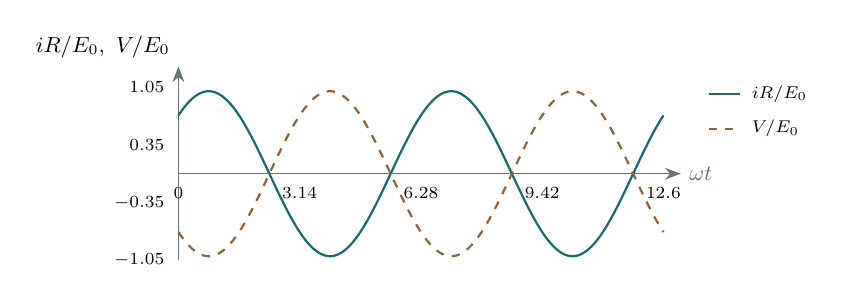
\begin{tikzpicture}[scale=.88,transform shape]
\draw[axis] (0,1.2500000)--(7.25,1.2500000) node[right] {$\omega t$};
\draw[axis] (0.0000000,0)--(0.0000000,2.8);
\node[above left] at (0.0000000,2.8) {$iR/E_0,\ V/E_0$};
\node[below,font=\scriptsize] at (0.0000000,1.1700000) {$0$};
\node[below,font=\scriptsize] at (1.7500000,1.1700000) {$3.14$};
\node[below,font=\scriptsize] at (3.5000000,1.1700000) {$6.28$};
\node[below,font=\scriptsize] at (5.2500000,1.1700000) {$9.42$};
\node[below,font=\scriptsize] at (7.0000000,1.1700000) {$12.6$};
\node[left,font=\scriptsize] at (-0.0800000,0.0000000) {$-1.05$};
\node[left,font=\scriptsize] at (-0.0800000,0.8333333) {$-0.35$};
\node[left,font=\scriptsize] at (-0.0800000,1.6666667) {$0.35$};
\node[left,font=\scriptsize] at (-0.0800000,2.5000000) {$1.05$};
\draw[thick,color=accent] plot coordinates {(0.0000000,2.0917938) (0.0273438,2.1320847) (0.0546875,2.1702505) (0.0820312,2.2061994) (0.1093750,2.2398448) (0.1367188,2.2711055) (0.1640625,2.2999063) (0.1914062,2.3261777) (0.2187500,2.3498566) (0.2460938,2.3708858) (0.2734375,2.3892147) (0.3007812,2.4047991) (0.3281250,2.4176015) (0.3554688,2.4275911) (0.3828125,2.4347437) (0.4101562,2.4390422) (0.4375000,2.4404762) (0.4648438,2.4390422) (0.4921875,2.4347437) (0.5195312,2.4275911) (0.5468750,2.4176015) (0.5742188,2.4047991) (0.6015625,2.3892147) (0.6289062,2.3708858) (0.6562500,2.3498566) (0.6835938,2.3261777) (0.7109375,2.2999063) (0.7382812,2.2711055) (0.7656250,2.2398448) (0.7929688,2.2061994) (0.8203125,2.1702505) (0.8476562,2.1320847) (0.8750000,2.0917938) (0.9023438,2.0494749) (0.9296875,2.0052301) (0.9570312,1.9591658) (0.9843750,1.9113931) (1.0117188,1.8620271) (1.0390625,1.8111866) (1.0664062,1.7589942) (1.0937500,1.7055755) (1.1210937,1.6510593) (1.1484375,1.5955770) (1.1757812,1.5392621) (1.2031250,1.4822504) (1.2304688,1.4246791) (1.2578125,1.3666871) (1.2851562,1.3084139) (1.3125000,1.2500000) (1.3398437,1.1915861) (1.3671875,1.1333129) (1.3945312,1.0753209) (1.4218750,1.0177496) (1.4492188,0.9607379) (1.4765625,0.9044230) (1.5039063,0.8489407) (1.5312500,0.7944245) (1.5585938,0.7410058) (1.5859375,0.6888134) (1.6132812,0.6379729) (1.6406250,0.5886069) (1.6679688,0.5408342) (1.6953125,0.4947699) (1.7226563,0.4505251) (1.7500000,0.4082062) (1.7773437,0.3679153) (1.8046875,0.3297495) (1.8320312,0.2938006) (1.8593750,0.2601552) (1.8867188,0.2288945) (1.9140625,0.2000937) (1.9414062,0.1738223) (1.9687500,0.1501434) (1.9960937,0.1291142) (2.0234375,0.1107853) (2.0507812,0.0952009) (2.0781250,0.0823985) (2.1054688,0.0724089) (2.1328125,0.0652563) (2.1601562,0.0609578) (2.1875000,0.0595238) (2.2148438,0.0609578) (2.2421875,0.0652563) (2.2695312,0.0724089) (2.2968750,0.0823985) (2.3242188,0.0952009) (2.3515625,0.1107853) (2.3789062,0.1291142) (2.4062500,0.1501434) (2.4335938,0.1738223) (2.4609375,0.2000937) (2.4882812,0.2288945) (2.5156250,0.2601552) (2.5429687,0.2938006) (2.5703125,0.3297495) (2.5976562,0.3679153) (2.6250000,0.4082062) (2.6523437,0.4505251) (2.6796875,0.4947699) (2.7070313,0.5408342) (2.7343750,0.5886069) (2.7617188,0.6379729) (2.7890625,0.6888134) (2.8164062,0.7410058) (2.8437500,0.7944245) (2.8710938,0.8489407) (2.8984375,0.9044230) (2.9257812,0.9607379) (2.9531250,1.0177496) (2.9804687,1.0753209) (3.0078125,1.1333129) (3.0351563,1.1915861) (3.0625000,1.2500000) (3.0898438,1.3084139) (3.1171875,1.3666871) (3.1445313,1.4246791) (3.1718750,1.4822504) (3.1992188,1.5392621) (3.2265625,1.5955770) (3.2539062,1.6510593) (3.2812500,1.7055755) (3.3085938,1.7589942) (3.3359375,1.8111866) (3.3632812,1.8620271) (3.3906250,1.9113931) (3.4179688,1.9591658) (3.4453125,2.0052301) (3.4726562,2.0494749) (3.5000000,2.0917938) (3.5273438,2.1320847) (3.5546875,2.1702505) (3.5820312,2.2061994) (3.6093750,2.2398448) (3.6367188,2.2711055) (3.6640625,2.2999063) (3.6914062,2.3261777) (3.7187500,2.3498566) (3.7460938,2.3708858) (3.7734375,2.3892147) (3.8007812,2.4047991) (3.8281250,2.4176015) (3.8554687,2.4275911) (3.8828125,2.4347437) (3.9101562,2.4390422) (3.9375000,2.4404762) (3.9648437,2.4390422) (3.9921875,2.4347437) (4.0195312,2.4275911) (4.0468750,2.4176015) (4.0742188,2.4047991) (4.1015625,2.3892147) (4.1289062,2.3708858) (4.1562500,2.3498566) (4.1835938,2.3261777) (4.2109375,2.2999063) (4.2382812,2.2711055) (4.2656250,2.2398448) (4.2929688,2.2061994) (4.3203125,2.1702505) (4.3476562,2.1320847) (4.3750000,2.0917938) (4.4023438,2.0494749) (4.4296875,2.0052301) (4.4570312,1.9591658) (4.4843750,1.9113931) (4.5117187,1.8620271) (4.5390625,1.8111866) (4.5664062,1.7589942) (4.5937500,1.7055755) (4.6210938,1.6510593) (4.6484375,1.5955770) (4.6757812,1.5392621) (4.7031250,1.4822504) (4.7304688,1.4246791) (4.7578125,1.3666871) (4.7851562,1.3084139) (4.8125000,1.2500000) (4.8398438,1.1915861) (4.8671875,1.1333129) (4.8945312,1.0753209) (4.9218750,1.0177496) (4.9492188,0.9607379) (4.9765625,0.9044230) (5.0039062,0.8489407) (5.0312500,0.7944245) (5.0585937,0.7410058) (5.0859375,0.6888134) (5.1132813,0.6379729) (5.1406250,0.5886069) (5.1679688,0.5408342) (5.1953125,0.4947699) (5.2226562,0.4505251) (5.2500000,0.4082062) (5.2773438,0.3679153) (5.3046875,0.3297495) (5.3320312,0.2938006) (5.3593750,0.2601552) (5.3867188,0.2288945) (5.4140625,0.2000937) (5.4414062,0.1738223) (5.4687500,0.1501434) (5.4960938,0.1291142) (5.5234375,0.1107853) (5.5507812,0.0952009) (5.5781250,0.0823985) (5.6054687,0.0724089) (5.6328125,0.0652563) (5.6601562,0.0609578) (5.6875000,0.0595238) (5.7148438,0.0609578) (5.7421875,0.0652563) (5.7695313,0.0724089) (5.7968750,0.0823985) (5.8242188,0.0952009) (5.8515625,0.1107853) (5.8789062,0.1291142) (5.9062500,0.1501434) (5.9335938,0.1738223) (5.9609375,0.2000937) (5.9882813,0.2288945) (6.0156250,0.2601552) (6.0429688,0.2938006) (6.0703125,0.3297495) (6.0976562,0.3679153) (6.1250000,0.4082062) (6.1523438,0.4505251) (6.1796875,0.4947699) (6.2070312,0.5408342) (6.2343750,0.5886069) (6.2617187,0.6379729) (6.2890625,0.6888134) (6.3164063,0.7410058) (6.3437500,0.7944245) (6.3710938,0.8489407) (6.3984375,0.9044230) (6.4257812,0.9607379) (6.4531250,1.0177496) (6.4804688,1.0753209) (6.5078125,1.1333129) (6.5351562,1.1915861) (6.5625000,1.2500000) (6.5898438,1.3084139) (6.6171875,1.3666871) (6.6445312,1.4246791) (6.6718750,1.4822504) (6.6992188,1.5392621) (6.7265625,1.5955770) (6.7539062,1.6510593) (6.7812500,1.7055755) (6.8085937,1.7589942) (6.8359375,1.8111866) (6.8632812,1.8620271) (6.8906250,1.9113931) (6.9179688,1.9591658) (6.9453125,2.0052301) (6.9726563,2.0494749) (7.0000000,2.0917938)};
\draw[thick,color=accent] (7.65,2.4)--(8.1,2.4);\node[right,font=\scriptsize] at (8.15,2.4) {$iR/E_0$};
\draw[thick,dashed,color=warm] plot coordinates {(0.0000000,0.4082062) (0.0273438,0.3679153) (0.0546875,0.3297495) (0.0820312,0.2938006) (0.1093750,0.2601552) (0.1367188,0.2288945) (0.1640625,0.2000937) (0.1914062,0.1738223) (0.2187500,0.1501434) (0.2460938,0.1291142) (0.2734375,0.1107853) (0.3007812,0.0952009) (0.3281250,0.0823985) (0.3554688,0.0724089) (0.3828125,0.0652563) (0.4101562,0.0609578) (0.4375000,0.0595238) (0.4648438,0.0609578) (0.4921875,0.0652563) (0.5195312,0.0724089) (0.5468750,0.0823985) (0.5742188,0.0952009) (0.6015625,0.1107853) (0.6289062,0.1291142) (0.6562500,0.1501434) (0.6835938,0.1738223) (0.7109375,0.2000937) (0.7382812,0.2288945) (0.7656250,0.2601552) (0.7929688,0.2938006) (0.8203125,0.3297495) (0.8476562,0.3679153) (0.8750000,0.4082062) (0.9023438,0.4505251) (0.9296875,0.4947699) (0.9570312,0.5408342) (0.9843750,0.5886069) (1.0117188,0.6379729) (1.0390625,0.6888134) (1.0664062,0.7410058) (1.0937500,0.7944245) (1.1210937,0.8489407) (1.1484375,0.9044230) (1.1757812,0.9607379) (1.2031250,1.0177496) (1.2304688,1.0753209) (1.2578125,1.1333129) (1.2851562,1.1915861) (1.3125000,1.2500000) (1.3398437,1.3084139) (1.3671875,1.3666871) (1.3945312,1.4246791) (1.4218750,1.4822504) (1.4492188,1.5392621) (1.4765625,1.5955770) (1.5039063,1.6510593) (1.5312500,1.7055755) (1.5585938,1.7589942) (1.5859375,1.8111866) (1.6132812,1.8620271) (1.6406250,1.9113931) (1.6679688,1.9591658) (1.6953125,2.0052301) (1.7226563,2.0494749) (1.7500000,2.0917938) (1.7773437,2.1320847) (1.8046875,2.1702505) (1.8320312,2.2061994) (1.8593750,2.2398448) (1.8867188,2.2711055) (1.9140625,2.2999063) (1.9414062,2.3261777) (1.9687500,2.3498566) (1.9960937,2.3708858) (2.0234375,2.3892147) (2.0507812,2.4047991) (2.0781250,2.4176015) (2.1054688,2.4275911) (2.1328125,2.4347437) (2.1601562,2.4390422) (2.1875000,2.4404762) (2.2148438,2.4390422) (2.2421875,2.4347437) (2.2695312,2.4275911) (2.2968750,2.4176015) (2.3242188,2.4047991) (2.3515625,2.3892147) (2.3789062,2.3708858) (2.4062500,2.3498566) (2.4335938,2.3261777) (2.4609375,2.2999063) (2.4882812,2.2711055) (2.5156250,2.2398448) (2.5429687,2.2061994) (2.5703125,2.1702505) (2.5976562,2.1320847) (2.6250000,2.0917938) (2.6523437,2.0494749) (2.6796875,2.0052301) (2.7070313,1.9591658) (2.7343750,1.9113931) (2.7617188,1.8620271) (2.7890625,1.8111866) (2.8164062,1.7589942) (2.8437500,1.7055755) (2.8710938,1.6510593) (2.8984375,1.5955770) (2.9257812,1.5392621) (2.9531250,1.4822504) (2.9804687,1.4246791) (3.0078125,1.3666871) (3.0351563,1.3084139) (3.0625000,1.2500000) (3.0898438,1.1915861) (3.1171875,1.1333129) (3.1445313,1.0753209) (3.1718750,1.0177496) (3.1992188,0.9607379) (3.2265625,0.9044230) (3.2539062,0.8489407) (3.2812500,0.7944245) (3.3085938,0.7410058) (3.3359375,0.6888134) (3.3632812,0.6379729) (3.3906250,0.5886069) (3.4179688,0.5408342) (3.4453125,0.4947699) (3.4726562,0.4505251) (3.5000000,0.4082062) (3.5273438,0.3679153) (3.5546875,0.3297495) (3.5820312,0.2938006) (3.6093750,0.2601552) (3.6367188,0.2288945) (3.6640625,0.2000937) (3.6914062,0.1738223) (3.7187500,0.1501434) (3.7460938,0.1291142) (3.7734375,0.1107853) (3.8007812,0.0952009) (3.8281250,0.0823985) (3.8554687,0.0724089) (3.8828125,0.0652563) (3.9101562,0.0609578) (3.9375000,0.0595238) (3.9648437,0.0609578) (3.9921875,0.0652563) (4.0195312,0.0724089) (4.0468750,0.0823985) (4.0742188,0.0952009) (4.1015625,0.1107853) (4.1289062,0.1291142) (4.1562500,0.1501434) (4.1835938,0.1738223) (4.2109375,0.2000937) (4.2382812,0.2288945) (4.2656250,0.2601552) (4.2929688,0.2938006) (4.3203125,0.3297495) (4.3476562,0.3679153) (4.3750000,0.4082062) (4.4023438,0.4505251) (4.4296875,0.4947699) (4.4570312,0.5408342) (4.4843750,0.5886069) (4.5117187,0.6379729) (4.5390625,0.6888134) (4.5664062,0.7410058) (4.5937500,0.7944245) (4.6210938,0.8489407) (4.6484375,0.9044230) (4.6757812,0.9607379) (4.7031250,1.0177496) (4.7304688,1.0753209) (4.7578125,1.1333129) (4.7851562,1.1915861) (4.8125000,1.2500000) (4.8398438,1.3084139) (4.8671875,1.3666871) (4.8945312,1.4246791) (4.9218750,1.4822504) (4.9492188,1.5392621) (4.9765625,1.5955770) (5.0039062,1.6510593) (5.0312500,1.7055755) (5.0585937,1.7589942) (5.0859375,1.8111866) (5.1132813,1.8620271) (5.1406250,1.9113931) (5.1679688,1.9591658) (5.1953125,2.0052301) (5.2226562,2.0494749) (5.2500000,2.0917938) (5.2773438,2.1320847) (5.3046875,2.1702505) (5.3320312,2.2061994) (5.3593750,2.2398448) (5.3867188,2.2711055) (5.4140625,2.2999063) (5.4414062,2.3261777) (5.4687500,2.3498566) (5.4960938,2.3708858) (5.5234375,2.3892147) (5.5507812,2.4047991) (5.5781250,2.4176015) (5.6054687,2.4275911) (5.6328125,2.4347437) (5.6601562,2.4390422) (5.6875000,2.4404762) (5.7148438,2.4390422) (5.7421875,2.4347437) (5.7695313,2.4275911) (5.7968750,2.4176015) (5.8242188,2.4047991) (5.8515625,2.3892147) (5.8789062,2.3708858) (5.9062500,2.3498566) (5.9335938,2.3261777) (5.9609375,2.2999063) (5.9882813,2.2711055) (6.0156250,2.2398448) (6.0429688,2.2061994) (6.0703125,2.1702505) (6.0976562,2.1320847) (6.1250000,2.0917938) (6.1523438,2.0494749) (6.1796875,2.0052301) (6.2070312,1.9591658) (6.2343750,1.9113931) (6.2617187,1.8620271) (6.2890625,1.8111866) (6.3164063,1.7589942) (6.3437500,1.7055755) (6.3710938,1.6510593) (6.3984375,1.5955770) (6.4257812,1.5392621) (6.4531250,1.4822504) (6.4804688,1.4246791) (6.5078125,1.3666871) (6.5351562,1.3084139) (6.5625000,1.2500000) (6.5898438,1.1915861) (6.6171875,1.1333129) (6.6445312,1.0753209) (6.6718750,1.0177496) (6.6992188,0.9607379) (6.7265625,0.9044230) (6.7539062,0.8489407) (6.7812500,0.7944245) (6.8085937,0.7410058) (6.8359375,0.6888134) (6.8632812,0.6379729) (6.8906250,0.5886069) (6.9179688,0.5408342) (6.9453125,0.4947699) (6.9726563,0.4505251) (7.0000000,0.4082062)};
\draw[thick,dashed,color=warm] (7.65,1.9)--(8.1,1.9);\node[right,font=\scriptsize] at (8.15,1.9) {$V/E_0$};
\end{tikzpicture}
\figcaption{变式图综一.4V1\quad 中频电阻电流与上节点电压反相。}
\end{minipage}\end{center}
\item 保持三个频率和峰值，把三个电源的初相位分别增加$\delta_1,\delta_2,\delta_3$，求电阻平均功率。每个等效图中的阻抗由频率决定，因此$I_n$只乘$e^{\mathrm j\delta_n}$，幅值保持$3E_0/(\sqrt{13}R),E_0/R,4E_0/(\sqrt{13}R)$。将$i^2$展开后，任意交叉项的频率仍为两分量的和、差；在$4\pi/\omega$内其积分为零。所以
\[
\bar P=\frac R2\sum_{n=1}^{3}|I_n|^2=\frac{19E_0^2}{13R}.
\]
图V2以三个$\delta_n$同取$\pi/3$为例，波形的峰谷位置已改变，整周期的平方积分相同。对某一有限时间段求电能时，直接积分该段的$Ri(t)^2$，便保留了这些相位带来的差别。
\begin{center}\begin{minipage}{.98\linewidth}\centering
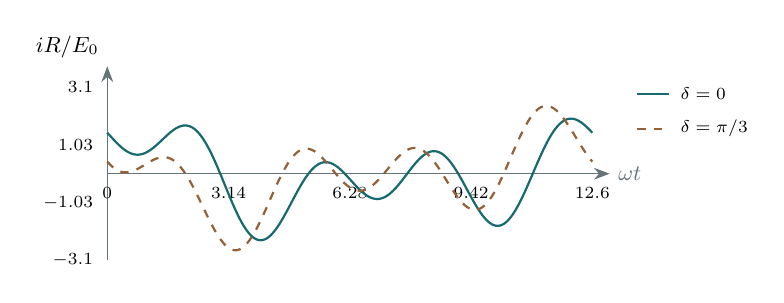
\begin{tikzpicture}[scale=.88,transform shape]
\draw[axis] (0,1.2500000)--(7.25,1.2500000) node[right] {$\omega t$};
\draw[axis] (0.0000000,0)--(0.0000000,2.8);
\node[above left] at (0.0000000,2.8) {$iR/E_0$};
\node[below,font=\scriptsize] at (0.0000000,1.1700000) {$0$};
\node[below,font=\scriptsize] at (1.7500000,1.1700000) {$3.14$};
\node[below,font=\scriptsize] at (3.5000000,1.1700000) {$6.28$};
\node[below,font=\scriptsize] at (5.2500000,1.1700000) {$9.42$};
\node[below,font=\scriptsize] at (7.0000000,1.1700000) {$12.6$};
\node[left,font=\scriptsize] at (-0.0800000,0.0000000) {$-3.1$};
\node[left,font=\scriptsize] at (-0.0800000,0.8333333) {$-1.03$};
\node[left,font=\scriptsize] at (-0.0800000,1.6666667) {$1.03$};
\node[left,font=\scriptsize] at (-0.0800000,2.5000000) {$3.1$};
\draw[thick,color=accent] plot coordinates {(0.0000000,1.8411419) (0.0273438,1.8116005) (0.0546875,1.7818348) (0.0820312,1.7522268) (0.1093750,1.7231497) (0.1367188,1.6949644) (0.1640625,1.6680153) (0.1914062,1.6426271) (0.2187500,1.6191015) (0.2460938,1.5977142) (0.2734375,1.5787118) (0.3007812,1.5623098) (0.3281250,1.5486898) (0.3554688,1.5379984) (0.3828125,1.5303451) (0.4101562,1.5258014) (0.4375000,1.5244004) (0.4648438,1.5261358) (0.4921875,1.5309626) (0.5195312,1.5387973) (0.5468750,1.5495188) (0.5742188,1.5629693) (0.6015625,1.5789564) (0.6289062,1.5972549) (0.6562500,1.6176089) (0.6835938,1.6397344) (0.7109375,1.6633225) (0.7382812,1.6880420) (0.7656250,1.7135435) (0.7929688,1.7394622) (0.8203125,1.7654221) (0.8476562,1.7910397) (0.8750000,1.8159280) (0.9023438,1.8397003) (0.9296875,1.8619744) (0.9570312,1.8823766) (0.9843750,1.9005452) (1.0117188,1.9161347) (1.0390625,1.9288194) (1.0664062,1.9382964) (1.0937500,1.9442897) (1.1210937,1.9465524) (1.1484375,1.9448697) (1.1757812,1.9390615) (1.2031250,1.9289843) (1.2304688,1.9145330) (1.2578125,1.8956423) (1.2851562,1.8722878) (1.3125000,1.8444863) (1.3398437,1.8122964) (1.3671875,1.7758182) (1.3945312,1.7351925) (1.4218750,1.6906002) (1.4492188,1.6422605) (1.4765625,1.5904297) (1.5039063,1.5353987) (1.5312500,1.4774906) (1.5585938,1.4170583) (1.5859375,1.3544809) (1.6132812,1.2901611) (1.6406250,1.2245209) (1.6679688,1.1579987) (1.6953125,1.0910447) (1.7226563,1.0241172) (1.7500000,0.9576787) (1.7773437,0.8921913) (1.8046875,0.8281130) (1.8320312,0.7658931) (1.8593750,0.7059687) (1.8867188,0.6487602) (1.9140625,0.5946678) (1.9414062,0.5440679) (1.9687500,0.4973095) (1.9960937,0.4547112) (2.0234375,0.4165582) (2.0507812,0.3830998) (2.0781250,0.3545473) (2.1054688,0.3310716) (2.1328125,0.3128023) (2.1601562,0.2998261) (2.1875000,0.2921862) (2.2148438,0.2898821) (2.2421875,0.2928694) (2.2695312,0.3010603) (2.2968750,0.3143248) (2.3242188,0.3324914) (2.3515625,0.3553493) (2.3789062,0.3826499) (2.4062500,0.4141094) (2.4335938,0.4494115) (2.4609375,0.4882103) (2.4882812,0.5301335) (2.5156250,0.5747858) (2.5429687,0.6217527) (2.5703125,0.6706044) (2.5976562,0.7208996) (2.6250000,0.7721897) (2.6523437,0.8240228) (2.6796875,0.8759481) (2.7070313,0.9275196) (2.7343750,0.9783007) (2.7617188,1.0278677) (2.7890625,1.0758140) (2.8164062,1.1217534) (2.8437500,1.1653238) (2.8710938,1.2061904) (2.8984375,1.2440484) (2.9257812,1.2786260) (2.9531250,1.3096865) (2.9804687,1.3370302) (3.0078125,1.3604962) (3.0351563,1.3799635) (3.0625000,1.3953519) (3.0898438,1.4066224) (3.1171875,1.4137774) (3.1445313,1.4168603) (3.1718750,1.4159545) (3.1992188,1.4111825) (3.2265625,1.4027046) (3.2539062,1.3907165) (3.2812500,1.3754477) (3.3085938,1.3571585) (3.3359375,1.3361374) (3.3632812,1.3126980) (3.3906250,1.2871757) (3.4179688,1.2599241) (3.4453125,1.2313113) (3.4726562,1.2017163) (3.5000000,1.1715247) (3.5273438,1.1411252) (3.5546875,1.1109052) (3.5820312,1.0812470) (3.6093750,1.0525240) (3.6367188,1.0250967) (3.6640625,0.9993090) (3.6914062,0.9754851) (3.7187500,0.9539257) (3.7460938,0.9349052) (3.7734375,0.9186690) (3.8007812,0.9054306) (3.8281250,0.8953700) (3.8554687,0.8886315) (3.8828125,0.8853222) (3.9101562,0.8855112) (3.9375000,0.8892284) (3.9648437,0.8964646) (3.9921875,0.9071716) (4.0195312,0.9212623) (4.0468750,0.9386116) (4.0742188,0.9590580) (4.1015625,0.9824048) (4.1289062,1.0084223) (4.1562500,1.0368499) (4.1835938,1.0673990) (4.2109375,1.0997553) (4.2382812,1.1335826) (4.2656250,1.1685258) (4.2929688,1.2042145) (4.3203125,1.2402668) (4.3476562,1.2762932) (4.3750000,1.3119003) (4.4023438,1.3466950) (4.4296875,1.3802886) (4.4570312,1.4123003) (4.4843750,1.4423616) (4.5117187,1.4701198) (4.5390625,1.4952418) (4.5664062,1.5174175) (4.5937500,1.5363628) (4.6210938,1.5518233) (4.6484375,1.5635761) (4.6757812,1.5714332) (4.7031250,1.5752426) (4.7304688,1.5748911) (4.7578125,1.5703048) (4.7851562,1.5614505) (4.8125000,1.5483366) (4.8398438,1.5310127) (4.8671875,1.5095698) (4.8945312,1.4841399) (4.9218750,1.4548945) (4.9492188,1.4220438) (4.9765625,1.3858346) (5.0039062,1.3465484) (5.0312500,1.3044990) (5.0585937,1.2600294) (5.0859375,1.2135095) (5.1132813,1.1653319) (5.1406250,1.1159093) (5.1679688,1.0656700) (5.1953125,1.0150545) (5.2226562,0.9645114) (5.2500000,0.9144931) (5.2773438,0.8654519) (5.3046875,0.8178359) (5.3320312,0.7720846) (5.3593750,0.7286250) (5.3867188,0.6878676) (5.4140625,0.6502028) (5.4414062,0.6159971) (5.4687500,0.5855895) (5.4960938,0.5592888) (5.5234375,0.5373705) (5.5507812,0.5200740) (5.5781250,0.5076008) (5.6054687,0.5001123) (5.6328125,0.4977284) (5.6601562,0.5005261) (5.6875000,0.5085393) (5.7148438,0.5217579) (5.7421875,0.5401282) (5.7695313,0.5635533) (5.7968750,0.5918938) (5.8242188,0.6249692) (5.8515625,0.6625597) (5.8789062,0.7044079) (5.9062500,0.7502212) (5.9335938,0.7996746) (5.9609375,0.8524138) (5.9882813,0.9080579) (6.0156250,0.9662035) (6.0429688,1.0264279) (6.0703125,1.0882934) (6.0976562,1.1513508) (6.1250000,1.2151437) (6.1523438,1.2792129) (6.1796875,1.3431000) (6.2070312,1.4063520) (6.2343750,1.4685251) (6.2617187,1.5291889) (6.2890625,1.5879299) (6.3164063,1.6443556) (6.3437500,1.6980975) (6.3710938,1.7488146) (6.3984375,1.7961963) (6.4257812,1.8399651) (6.4531250,1.8798786) (6.4804688,1.9157318) (6.5078125,1.9473587) (6.5351562,1.9746334) (6.5625000,1.9974710) (6.5898438,2.0158281) (6.6171875,2.0297027) (6.6445312,2.0391341) (6.6718750,2.0442020) (6.6992188,2.0450253) (6.7265625,2.0417609) (6.7539062,2.0346014) (6.7812500,2.0237733) (6.8085937,2.0095342) (6.8359375,1.9921703) (6.8632812,1.9719930) (6.8906250,1.9493356) (6.9179688,1.9245500) (6.9453125,1.8980029) (6.9726563,1.8700719) (7.0000000,1.8411419)};
\draw[thick,color=accent] (7.65,2.4)--(8.1,2.4);\node[right,font=\scriptsize] at (8.15,2.4) {$\delta=0$};
\draw[thick,dashed,color=warm] plot coordinates {(0.0000000,1.4245916) (0.0273438,1.3945915) (0.0546875,1.3675891) (0.0820312,1.3437340) (0.1093750,1.3231380) (0.1367188,1.3058743) (0.1640625,1.2919768) (0.1914062,1.2814400) (0.2187500,1.2742193) (0.2460938,1.2702317) (0.2734375,1.2693569) (0.3007812,1.2714384) (0.3281250,1.2762856) (0.3554688,1.2836758) (0.3828125,1.2933567) (0.4101562,1.3050491) (0.4375000,1.3184498) (0.4648438,1.3332351) (0.4921875,1.3490639) (0.5195312,1.3655818) (0.5468750,1.3824243) (0.5742188,1.3992213) (0.6015625,1.4156004) (0.6289062,1.4311913) (0.6562500,1.4456298) (0.6835938,1.4585611) (0.7109375,1.4696443) (0.7382812,1.4785558) (0.7656250,1.4849924) (0.7929688,1.4886755) (0.8203125,1.4893533) (0.8476562,1.4868040) (0.8750000,1.4808386) (0.9023438,1.4713023) (0.9296875,1.4580773) (0.9570312,1.4410836) (0.9843750,1.4202805) (1.0117188,1.3956674) (1.0390625,1.3672838) (1.0664062,1.3352095) (1.0937500,1.2995645) (1.1210937,1.2605074) (1.1484375,1.2182348) (1.1757812,1.1729798) (1.2031250,1.1250093) (1.2304688,1.0746227) (1.2578125,1.0221484) (1.2851562,0.9679417) (1.3125000,0.9123809) (1.3398437,0.8558643) (1.3671875,0.7988066) (1.3945312,0.7416349) (1.4218750,0.6847849) (1.4492188,0.6286968) (1.4765625,0.5738115) (1.5039063,0.5205659) (1.5312500,0.4693894) (1.5585938,0.4206995) (1.5859375,0.3748983) (1.6132812,0.3323680) (1.6406250,0.2934678) (1.6679688,0.2585304) (1.6953125,0.2278588) (1.7226563,0.2017232) (1.7500000,0.1803586) (1.7773437,0.1639622) (1.8046875,0.1526920) (1.8320312,0.1466645) (1.8593750,0.1459540) (1.8867188,0.1505917) (1.9140625,0.1605651) (1.9414062,0.1758180) (1.9687500,0.1962511) (1.9960937,0.2217226) (2.0234375,0.2520494) (2.0507812,0.2870088) (2.0781250,0.3263401) (2.1054688,0.3697474) (2.1328125,0.4169016) (2.1601562,0.4674440) (2.1875000,0.5209888) (2.2148438,0.5771270) (2.2421875,0.6354300) (2.2695312,0.6954532) (2.2968750,0.7567402) (2.3242188,0.8188269) (2.3515625,0.8812454) (2.3789062,0.9435285) (2.4062500,1.0052137) (2.4335938,1.0658472) (2.4609375,1.1249883) (2.4882812,1.1822128) (2.5156250,1.2371172) (2.5429687,1.2893221) (2.5703125,1.3384752) (2.5976562,1.3842549) (2.6250000,1.4263725) (2.6523437,1.4645750) (2.6796875,1.4986471) (2.7070313,1.5284128) (2.7343750,1.5537370) (2.7617188,1.5745264) (2.7890625,1.5907297) (2.8164062,1.6023384) (2.8437500,1.6093862) (2.8710938,1.6119483) (2.8984375,1.6101407) (2.9257812,1.6041184) (2.9531250,1.5940741) (2.9804687,1.5802355) (3.0078125,1.5628636) (3.0351563,1.5422490) (3.0625000,1.5187099) (3.0898438,1.4925879) (3.1171875,1.4642453) (3.1445313,1.4340606) (3.1718750,1.4024255) (3.1992188,1.3697404) (3.2265625,1.3364105) (3.2539062,1.3028420) (3.2812500,1.2694380) (3.3085938,1.2365941) (3.3359375,1.2046952) (3.3632812,1.1741111) (3.3906250,1.1451932) (3.4179688,1.1182713) (3.4453125,1.0936497) (3.4726562,1.0716050) (3.5000000,1.0523831) (3.5273438,1.0361969) (3.5546875,1.0232241) (3.5820312,1.0136061) (3.6093750,1.0074460) (3.6367188,1.0048084) (3.6640625,1.0057184) (3.6914062,1.0101615) (3.7187500,1.0180841) (3.7460938,1.0293942) (3.7734375,1.0439620) (3.8007812,1.0616219) (3.8281250,1.0821739) (3.8554687,1.1053859) (3.8828125,1.1309959) (3.9101562,1.1587152) (3.9375000,1.1882310) (3.9648437,1.2192098) (3.9921875,1.2513009) (4.0195312,1.2841398) (4.0468750,1.3173525) (4.0742188,1.3505588) (4.1015625,1.3833766) (4.1289062,1.4154257) (4.1562500,1.4463317) (4.1835938,1.4757301) (4.2109375,1.5032702) (4.2382812,1.5286181) (4.2656250,1.5514612) (4.2929688,1.5715106) (4.3203125,1.5885049) (4.3476562,1.6022124) (4.3750000,1.6124341) (4.4023438,1.6190058) (4.4296875,1.6217998) (4.4570312,1.6207264) (4.4843750,1.6157355) (4.5117187,1.6068168) (4.5390625,1.5940004) (4.5664062,1.5773568) (4.5937500,1.5569966) (4.6210938,1.5330692) (4.6484375,1.5057622) (4.6757812,1.4752995) (4.7031250,1.4419393) (4.7304688,1.4059720) (4.7578125,1.3677175) (4.7851562,1.3275223) (4.8125000,1.2857565) (4.8398438,1.2428100) (4.8671875,1.1990893) (4.8945312,1.1550135) (4.9218750,1.1110104) (4.9492188,1.0675125) (4.9765625,1.0249529) (5.0039062,0.9837614) (5.0312500,0.9443599) (5.0585937,0.9071591) (5.0859375,0.8725537) (5.1132813,0.8409195) (5.1406250,0.8126092) (5.1679688,0.7879490) (5.1953125,0.7672356) (5.2226562,0.7507333) (5.2500000,0.7386712) (5.2773438,0.7312412) (5.3046875,0.7285955) (5.3320312,0.7308457) (5.3593750,0.7380610) (5.3867188,0.7502679) (5.4140625,0.7674492) (5.4414062,0.7895444) (5.4687500,0.8164502) (5.4960938,0.8480208) (5.5234375,0.8840694) (5.5507812,0.9243699) (5.5781250,0.9686584) (5.6054687,1.0166359) (5.6328125,1.0679708) (5.6601562,1.1223017) (5.6875000,1.1792404) (5.7148438,1.2383761) (5.7421875,1.2992783) (5.7695313,1.3615008) (5.7968750,1.4245859) (5.8242188,1.4880683) (5.8515625,1.5514795) (5.8789062,1.6143516) (5.9062500,1.6762216) (5.9335938,1.7366358) (5.9609375,1.7951535) (5.9882813,1.8513510) (6.0156250,1.9048253) (6.0429688,1.9551978) (6.0703125,2.0021175) (6.0976562,2.0452640) (6.1250000,2.0843503) (6.1523438,2.1191251) (6.1796875,2.1493752) (6.2070312,2.1749270) (6.2343750,2.1956479) (6.2617187,2.2114471) (6.2890625,2.2222768) (6.3164063,2.2281314) (6.3437500,2.2290481) (6.3710938,2.2251059) (6.3984375,2.2164246) (6.4257812,2.2031634) (6.4531250,2.1855194) (6.4804688,2.1637248) (6.5078125,2.1380454) (6.5351562,2.1087770) (6.5625000,2.0762427) (6.5898438,2.0407897) (6.6171875,2.0027858) (6.6445312,1.9626155) (6.6718750,1.9206764) (6.6992188,1.8773750) (6.7265625,1.8331232) (6.7539062,1.7883336) (6.7812500,1.7434159) (6.8085937,1.6987730) (6.8359375,1.6547965) (6.8632812,1.6118638) (6.8906250,1.5703336) (6.9179688,1.5305432) (6.9453125,1.4928049) (6.9726563,1.4574031) (7.0000000,1.4245916)};
\draw[thick,dashed,color=warm] (7.65,1.9)--(8.1,1.9);\node[right,font=\scriptsize] at (8.15,1.9) {$\delta=\pi/3$};
\end{tikzpicture}
\figcaption{变式图综一.4V2\quad 各电源初相位同时增加60度后的波形。}
\end{minipage}\end{center}
\item 把三个电源峰值同时乘以实数$a$，并讨论将$E_0$定义为有效值的记法。线性节点式中$V$和每个支路电流同时乘$a$，故$i_a(t)=a i(t)$，$\bar P_a=a^2\bar P$。图V3的$a=1/2$对应
\[
i_{1/2}=\tfrac12i,\qquad \bar P_{1/2}=\frac{19E_0^2}{52R}.
\]
若三个电源各自的有效值为$E_0$，则用于峰值相量式的幅度为$\sqrt2E_0$，平均功率为$38E_0^2/(13R)$。这个因子来自正弦平方平均$1/2$：有效值已把此因子吸收入定义，图中纵坐标的实际峰值相应增加$\sqrt2$倍。
\begin{center}\begin{minipage}{.98\linewidth}\centering
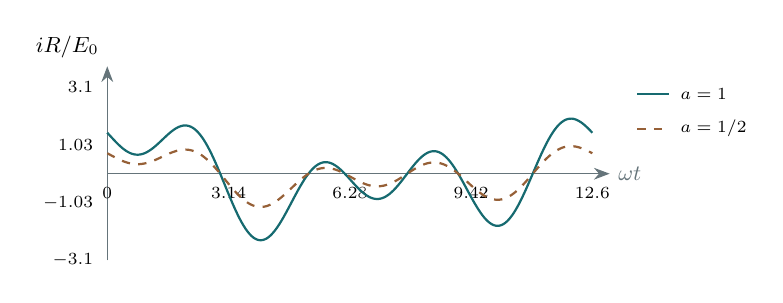
\begin{tikzpicture}[scale=.88,transform shape]
\draw[axis] (0,1.2500000)--(7.25,1.2500000) node[right] {$\omega t$};
\draw[axis] (0.0000000,0)--(0.0000000,2.8);
\node[above left] at (0.0000000,2.8) {$iR/E_0$};
\node[below,font=\scriptsize] at (0.0000000,1.1700000) {$0$};
\node[below,font=\scriptsize] at (1.7500000,1.1700000) {$3.14$};
\node[below,font=\scriptsize] at (3.5000000,1.1700000) {$6.28$};
\node[below,font=\scriptsize] at (5.2500000,1.1700000) {$9.42$};
\node[below,font=\scriptsize] at (7.0000000,1.1700000) {$12.6$};
\node[left,font=\scriptsize] at (-0.0800000,0.0000000) {$-3.1$};
\node[left,font=\scriptsize] at (-0.0800000,0.8333333) {$-1.03$};
\node[left,font=\scriptsize] at (-0.0800000,1.6666667) {$1.03$};
\node[left,font=\scriptsize] at (-0.0800000,2.5000000) {$3.1$};
\draw[thick,color=accent] plot coordinates {(0.0000000,1.8411419) (0.0273438,1.8116005) (0.0546875,1.7818348) (0.0820312,1.7522268) (0.1093750,1.7231497) (0.1367188,1.6949644) (0.1640625,1.6680153) (0.1914062,1.6426271) (0.2187500,1.6191015) (0.2460938,1.5977142) (0.2734375,1.5787118) (0.3007812,1.5623098) (0.3281250,1.5486898) (0.3554688,1.5379984) (0.3828125,1.5303451) (0.4101562,1.5258014) (0.4375000,1.5244004) (0.4648438,1.5261358) (0.4921875,1.5309626) (0.5195312,1.5387973) (0.5468750,1.5495188) (0.5742188,1.5629693) (0.6015625,1.5789564) (0.6289062,1.5972549) (0.6562500,1.6176089) (0.6835938,1.6397344) (0.7109375,1.6633225) (0.7382812,1.6880420) (0.7656250,1.7135435) (0.7929688,1.7394622) (0.8203125,1.7654221) (0.8476562,1.7910397) (0.8750000,1.8159280) (0.9023438,1.8397003) (0.9296875,1.8619744) (0.9570312,1.8823766) (0.9843750,1.9005452) (1.0117188,1.9161347) (1.0390625,1.9288194) (1.0664062,1.9382964) (1.0937500,1.9442897) (1.1210937,1.9465524) (1.1484375,1.9448697) (1.1757812,1.9390615) (1.2031250,1.9289843) (1.2304688,1.9145330) (1.2578125,1.8956423) (1.2851562,1.8722878) (1.3125000,1.8444863) (1.3398437,1.8122964) (1.3671875,1.7758182) (1.3945312,1.7351925) (1.4218750,1.6906002) (1.4492188,1.6422605) (1.4765625,1.5904297) (1.5039063,1.5353987) (1.5312500,1.4774906) (1.5585938,1.4170583) (1.5859375,1.3544809) (1.6132812,1.2901611) (1.6406250,1.2245209) (1.6679688,1.1579987) (1.6953125,1.0910447) (1.7226563,1.0241172) (1.7500000,0.9576787) (1.7773437,0.8921913) (1.8046875,0.8281130) (1.8320312,0.7658931) (1.8593750,0.7059687) (1.8867188,0.6487602) (1.9140625,0.5946678) (1.9414062,0.5440679) (1.9687500,0.4973095) (1.9960937,0.4547112) (2.0234375,0.4165582) (2.0507812,0.3830998) (2.0781250,0.3545473) (2.1054688,0.3310716) (2.1328125,0.3128023) (2.1601562,0.2998261) (2.1875000,0.2921862) (2.2148438,0.2898821) (2.2421875,0.2928694) (2.2695312,0.3010603) (2.2968750,0.3143248) (2.3242188,0.3324914) (2.3515625,0.3553493) (2.3789062,0.3826499) (2.4062500,0.4141094) (2.4335938,0.4494115) (2.4609375,0.4882103) (2.4882812,0.5301335) (2.5156250,0.5747858) (2.5429687,0.6217527) (2.5703125,0.6706044) (2.5976562,0.7208996) (2.6250000,0.7721897) (2.6523437,0.8240228) (2.6796875,0.8759481) (2.7070313,0.9275196) (2.7343750,0.9783007) (2.7617188,1.0278677) (2.7890625,1.0758140) (2.8164062,1.1217534) (2.8437500,1.1653238) (2.8710938,1.2061904) (2.8984375,1.2440484) (2.9257812,1.2786260) (2.9531250,1.3096865) (2.9804687,1.3370302) (3.0078125,1.3604962) (3.0351563,1.3799635) (3.0625000,1.3953519) (3.0898438,1.4066224) (3.1171875,1.4137774) (3.1445313,1.4168603) (3.1718750,1.4159545) (3.1992188,1.4111825) (3.2265625,1.4027046) (3.2539062,1.3907165) (3.2812500,1.3754477) (3.3085938,1.3571585) (3.3359375,1.3361374) (3.3632812,1.3126980) (3.3906250,1.2871757) (3.4179688,1.2599241) (3.4453125,1.2313113) (3.4726562,1.2017163) (3.5000000,1.1715247) (3.5273438,1.1411252) (3.5546875,1.1109052) (3.5820312,1.0812470) (3.6093750,1.0525240) (3.6367188,1.0250967) (3.6640625,0.9993090) (3.6914062,0.9754851) (3.7187500,0.9539257) (3.7460938,0.9349052) (3.7734375,0.9186690) (3.8007812,0.9054306) (3.8281250,0.8953700) (3.8554687,0.8886315) (3.8828125,0.8853222) (3.9101562,0.8855112) (3.9375000,0.8892284) (3.9648437,0.8964646) (3.9921875,0.9071716) (4.0195312,0.9212623) (4.0468750,0.9386116) (4.0742188,0.9590580) (4.1015625,0.9824048) (4.1289062,1.0084223) (4.1562500,1.0368499) (4.1835938,1.0673990) (4.2109375,1.0997553) (4.2382812,1.1335826) (4.2656250,1.1685258) (4.2929688,1.2042145) (4.3203125,1.2402668) (4.3476562,1.2762932) (4.3750000,1.3119003) (4.4023438,1.3466950) (4.4296875,1.3802886) (4.4570312,1.4123003) (4.4843750,1.4423616) (4.5117187,1.4701198) (4.5390625,1.4952418) (4.5664062,1.5174175) (4.5937500,1.5363628) (4.6210938,1.5518233) (4.6484375,1.5635761) (4.6757812,1.5714332) (4.7031250,1.5752426) (4.7304688,1.5748911) (4.7578125,1.5703048) (4.7851562,1.5614505) (4.8125000,1.5483366) (4.8398438,1.5310127) (4.8671875,1.5095698) (4.8945312,1.4841399) (4.9218750,1.4548945) (4.9492188,1.4220438) (4.9765625,1.3858346) (5.0039062,1.3465484) (5.0312500,1.3044990) (5.0585937,1.2600294) (5.0859375,1.2135095) (5.1132813,1.1653319) (5.1406250,1.1159093) (5.1679688,1.0656700) (5.1953125,1.0150545) (5.2226562,0.9645114) (5.2500000,0.9144931) (5.2773438,0.8654519) (5.3046875,0.8178359) (5.3320312,0.7720846) (5.3593750,0.7286250) (5.3867188,0.6878676) (5.4140625,0.6502028) (5.4414062,0.6159971) (5.4687500,0.5855895) (5.4960938,0.5592888) (5.5234375,0.5373705) (5.5507812,0.5200740) (5.5781250,0.5076008) (5.6054687,0.5001123) (5.6328125,0.4977284) (5.6601562,0.5005261) (5.6875000,0.5085393) (5.7148438,0.5217579) (5.7421875,0.5401282) (5.7695313,0.5635533) (5.7968750,0.5918938) (5.8242188,0.6249692) (5.8515625,0.6625597) (5.8789062,0.7044079) (5.9062500,0.7502212) (5.9335938,0.7996746) (5.9609375,0.8524138) (5.9882813,0.9080579) (6.0156250,0.9662035) (6.0429688,1.0264279) (6.0703125,1.0882934) (6.0976562,1.1513508) (6.1250000,1.2151437) (6.1523438,1.2792129) (6.1796875,1.3431000) (6.2070312,1.4063520) (6.2343750,1.4685251) (6.2617187,1.5291889) (6.2890625,1.5879299) (6.3164063,1.6443556) (6.3437500,1.6980975) (6.3710938,1.7488146) (6.3984375,1.7961963) (6.4257812,1.8399651) (6.4531250,1.8798786) (6.4804688,1.9157318) (6.5078125,1.9473587) (6.5351562,1.9746334) (6.5625000,1.9974710) (6.5898438,2.0158281) (6.6171875,2.0297027) (6.6445312,2.0391341) (6.6718750,2.0442020) (6.6992188,2.0450253) (6.7265625,2.0417609) (6.7539062,2.0346014) (6.7812500,2.0237733) (6.8085937,2.0095342) (6.8359375,1.9921703) (6.8632812,1.9719930) (6.8906250,1.9493356) (6.9179688,1.9245500) (6.9453125,1.8980029) (6.9726563,1.8700719) (7.0000000,1.8411419)};
\draw[thick,color=accent] (7.65,2.4)--(8.1,2.4);\node[right,font=\scriptsize] at (8.15,2.4) {$a=1$};
\draw[thick,dashed,color=warm] plot coordinates {(0.0000000,1.5455709) (0.0273438,1.5308003) (0.0546875,1.5159174) (0.0820312,1.5011134) (0.1093750,1.4865749) (0.1367188,1.4724822) (0.1640625,1.4590076) (0.1914062,1.4463135) (0.2187500,1.4345507) (0.2460938,1.4238571) (0.2734375,1.4143559) (0.3007812,1.4061549) (0.3281250,1.3993449) (0.3554688,1.3939992) (0.3828125,1.3901725) (0.4101562,1.3879007) (0.4375000,1.3872002) (0.4648438,1.3880679) (0.4921875,1.3904813) (0.5195312,1.3943987) (0.5468750,1.3997594) (0.5742188,1.4064846) (0.6015625,1.4144782) (0.6289062,1.4236275) (0.6562500,1.4338045) (0.6835938,1.4448672) (0.7109375,1.4566612) (0.7382812,1.4690210) (0.7656250,1.4817717) (0.7929688,1.4947311) (0.8203125,1.5077110) (0.8476562,1.5205198) (0.8750000,1.5329640) (0.9023438,1.5448501) (0.9296875,1.5559872) (0.9570312,1.5661883) (0.9843750,1.5752726) (1.0117188,1.5830674) (1.0390625,1.5894097) (1.0664062,1.5941482) (1.0937500,1.5971449) (1.1210937,1.5982762) (1.1484375,1.5974349) (1.1757812,1.5945308) (1.2031250,1.5894922) (1.2304688,1.5822665) (1.2578125,1.5728212) (1.2851562,1.5611439) (1.3125000,1.5472431) (1.3398437,1.5311482) (1.3671875,1.5129091) (1.3945312,1.4925963) (1.4218750,1.4703001) (1.4492188,1.4461303) (1.4765625,1.4202149) (1.5039063,1.3926994) (1.5312500,1.3637453) (1.5585938,1.3335292) (1.5859375,1.3022405) (1.6132812,1.2700805) (1.6406250,1.2372605) (1.6679688,1.2039994) (1.6953125,1.1705223) (1.7226563,1.1370586) (1.7500000,1.1038393) (1.7773437,1.0710957) (1.8046875,1.0390565) (1.8320312,1.0079466) (1.8593750,0.9779844) (1.8867188,0.9493801) (1.9140625,0.9223339) (1.9414062,0.8970339) (1.9687500,0.8736547) (1.9960937,0.8523556) (2.0234375,0.8332791) (2.0507812,0.8165499) (2.0781250,0.8022736) (2.1054688,0.7905358) (2.1328125,0.7814012) (2.1601562,0.7749130) (2.1875000,0.7710931) (2.2148438,0.7699410) (2.2421875,0.7714347) (2.2695312,0.7755302) (2.2968750,0.7821624) (2.3242188,0.7912457) (2.3515625,0.8026746) (2.3789062,0.8163249) (2.4062500,0.8320547) (2.4335938,0.8497058) (2.4609375,0.8691052) (2.4882812,0.8900667) (2.5156250,0.9123929) (2.5429687,0.9358764) (2.5703125,0.9603022) (2.5976562,0.9854498) (2.6250000,1.0110949) (2.6523437,1.0370114) (2.6796875,1.0629740) (2.7070313,1.0887598) (2.7343750,1.1141503) (2.7617188,1.1389339) (2.7890625,1.1629070) (2.8164062,1.1858767) (2.8437500,1.2076619) (2.8710938,1.2280952) (2.8984375,1.2470242) (2.9257812,1.2643130) (2.9531250,1.2798433) (2.9804687,1.2935151) (3.0078125,1.3052481) (3.0351563,1.3149817) (3.0625000,1.3226759) (3.0898438,1.3283112) (3.1171875,1.3318887) (3.1445313,1.3334301) (3.1718750,1.3329772) (3.1992188,1.3305912) (3.2265625,1.3263523) (3.2539062,1.3203583) (3.2812500,1.3127239) (3.3085938,1.3035793) (3.3359375,1.2930687) (3.3632812,1.2813490) (3.3906250,1.2685879) (3.4179688,1.2549620) (3.4453125,1.2406556) (3.4726562,1.2258581) (3.5000000,1.2107623) (3.5273438,1.1955626) (3.5546875,1.1804526) (3.5820312,1.1656235) (3.6093750,1.1512620) (3.6367188,1.1375483) (3.6640625,1.1246545) (3.6914062,1.1127426) (3.7187500,1.1019629) (3.7460938,1.0924526) (3.7734375,1.0843345) (3.8007812,1.0777153) (3.8281250,1.0726850) (3.8554687,1.0693158) (3.8828125,1.0676611) (3.9101562,1.0677556) (3.9375000,1.0696142) (3.9648437,1.0732323) (3.9921875,1.0785858) (4.0195312,1.0856311) (4.0468750,1.0943058) (4.0742188,1.1045290) (4.1015625,1.1162024) (4.1289062,1.1292111) (4.1562500,1.1434250) (4.1835938,1.1586995) (4.2109375,1.1748776) (4.2382812,1.1917913) (4.2656250,1.2092629) (4.2929688,1.2271072) (4.3203125,1.2451334) (4.3476562,1.2631466) (4.3750000,1.2809501) (4.4023438,1.2983475) (4.4296875,1.3151443) (4.4570312,1.3311502) (4.4843750,1.3461808) (4.5117187,1.3600599) (4.5390625,1.3726209) (4.5664062,1.3837087) (4.5937500,1.3931814) (4.6210938,1.4009116) (4.6484375,1.4067881) (4.6757812,1.4107166) (4.7031250,1.4126213) (4.7304688,1.4124455) (4.7578125,1.4101524) (4.7851562,1.4057253) (4.8125000,1.3991683) (4.8398438,1.3905063) (4.8671875,1.3797849) (4.8945312,1.3670699) (4.9218750,1.3524472) (4.9492188,1.3360219) (4.9765625,1.3179173) (5.0039062,1.2982742) (5.0312500,1.2772495) (5.0585937,1.2550147) (5.0859375,1.2317547) (5.1132813,1.2076660) (5.1406250,1.1829547) (5.1679688,1.1578350) (5.1953125,1.1325272) (5.2226562,1.1072557) (5.2500000,1.0822465) (5.2773438,1.0577260) (5.3046875,1.0339180) (5.3320312,1.0110423) (5.3593750,0.9893125) (5.3867188,0.9689338) (5.4140625,0.9501014) (5.4414062,0.9329985) (5.4687500,0.9177947) (5.4960938,0.9046444) (5.5234375,0.8936852) (5.5507812,0.8850370) (5.5781250,0.8788004) (5.6054687,0.8750562) (5.6328125,0.8738642) (5.6601562,0.8752630) (5.6875000,0.8792696) (5.7148438,0.8858790) (5.7421875,0.8950641) (5.7695313,0.9067767) (5.7968750,0.9209469) (5.8242188,0.9374846) (5.8515625,0.9562799) (5.8789062,0.9772040) (5.9062500,1.0001106) (5.9335938,1.0248373) (5.9609375,1.0512069) (5.9882813,1.0790289) (6.0156250,1.1081017) (6.0429688,1.1382140) (6.0703125,1.1691467) (6.0976562,1.2006754) (6.1250000,1.2325719) (6.1523438,1.2646064) (6.1796875,1.2965500) (6.2070312,1.3281760) (6.2343750,1.3592625) (6.2617187,1.3895944) (6.2890625,1.4189649) (6.3164063,1.4471778) (6.3437500,1.4740487) (6.3710938,1.4994073) (6.3984375,1.5230982) (6.4257812,1.5449826) (6.4531250,1.5649393) (6.4804688,1.5828659) (6.5078125,1.5986794) (6.5351562,1.6123167) (6.5625000,1.6237355) (6.5898438,1.6329140) (6.6171875,1.6398514) (6.6445312,1.6445671) (6.6718750,1.6471010) (6.6992188,1.6475127) (6.7265625,1.6458804) (6.7539062,1.6423007) (6.7812500,1.6368866) (6.8085937,1.6297671) (6.8359375,1.6210852) (6.8632812,1.6109965) (6.8906250,1.5996678) (6.9179688,1.5872750) (6.9453125,1.5740014) (6.9726563,1.5600360) (7.0000000,1.5455709)};
\draw[thick,dashed,color=warm] (7.65,1.9)--(8.1,1.9);\node[right,font=\scriptsize] at (8.15,1.9) {$a=1/2$};
\end{tikzpicture}
\figcaption{变式图综一.4V3\quad 电源峰值减半，电流纵坐标随之减半。}
\end{minipage}\end{center}
\item 将全部电源短路，求自由暂态，并说明两个初始储能条件怎样进入。节点的向下电流满足$V/R+i_L+C\dot V=0$，电感有$L\dot i_L=V$。对节点式求导后消去$i_L$，得
\[
LC\ddot V+(L/R)\dot V+V=0,\qquad
\ddot V+\omega\dot V+\omega^2V=0.
\]
特征根$-\omega/2\pm\mathrm j\sqrt3\omega/2$，所以
\[
V_{\rm tr}=e^{-\omega t/2}[A\cos(\sqrt3\omega t/2)+B\sin(\sqrt3\omega t/2)].
\]
$A=V_{\rm tr}(0)$由初始电容电压确定；由$\dot V(0)=-V(0)/(RC)-i_L(0)/C$求得$B=2[\dot V(0)+\omega A/2]/(\sqrt3\omega)$。有驱动时先减去稳态初值再用这一关系。图V4取$A=V_a,B=0$，归一化电压$V_{\rm tr}/V_a$在$\pm e^{-\omega t/2}$包络中衰减，其长期平均功率贡献趋于零。
\begin{center}\begin{minipage}{.98\linewidth}\centering
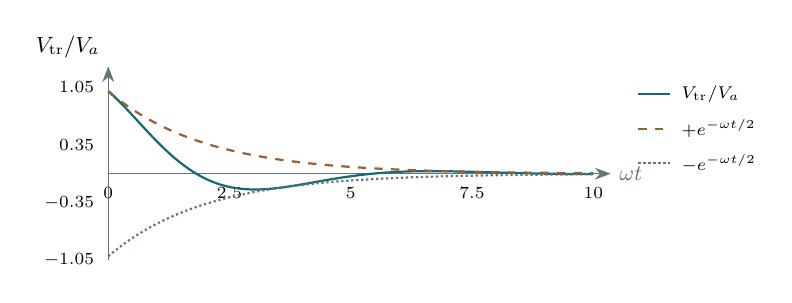
\begin{tikzpicture}[scale=.88,transform shape]
\draw[axis] (0,1.2500000)--(7.25,1.2500000) node[right] {$\omega t$};
\draw[axis] (0.0000000,0)--(0.0000000,2.8);
\node[above left] at (0.0000000,2.8) {$V_{\rm tr}/V_a$};
\node[below,font=\scriptsize] at (0.0000000,1.1700000) {$0$};
\node[below,font=\scriptsize] at (1.7500000,1.1700000) {$2.5$};
\node[below,font=\scriptsize] at (3.5000000,1.1700000) {$5$};
\node[below,font=\scriptsize] at (5.2500000,1.1700000) {$7.5$};
\node[below,font=\scriptsize] at (7.0000000,1.1700000) {$10$};
\node[left,font=\scriptsize] at (-0.0800000,0.0000000) {$-1.05$};
\node[left,font=\scriptsize] at (-0.0800000,0.8333333) {$-0.35$};
\node[left,font=\scriptsize] at (-0.0800000,1.6666667) {$0.35$};
\node[left,font=\scriptsize] at (-0.0800000,2.5000000) {$1.05$};
\draw[thick,color=accent] plot coordinates {(0.0000000,2.4404762) (0.0291667,2.4151722) (0.0583333,2.3889198) (0.0875000,2.3618025) (0.1166667,2.3339015) (0.1458333,2.3052963) (0.1750000,2.2760643) (0.2041667,2.2462808) (0.2333333,2.2160189) (0.2625000,2.1853496) (0.2916667,2.1543417) (0.3208333,2.1230616) (0.3500000,2.0915737) (0.3791667,2.0599400) (0.4083333,2.0282203) (0.4375000,1.9964719) (0.4666667,1.9647501) (0.4958333,1.9331076) (0.5250000,1.9015950) (0.5541667,1.8702607) (0.5833333,1.8391506) (0.6125000,1.8083084) (0.6416667,1.7777757) (0.6708333,1.7475917) (0.7000000,1.7177935) (0.7291667,1.6884161) (0.7583333,1.6594922) (0.7875000,1.6310525) (0.8166667,1.6031255) (0.8458333,1.5757379) (0.8750000,1.5489142) (0.9041667,1.5226769) (0.9333333,1.4970468) (0.9625000,1.4720427) (0.9916667,1.4476814) (1.0208333,1.4239783) (1.0500000,1.4009467) (1.0791667,1.3785984) (1.1083333,1.3569435) (1.1375000,1.3359906) (1.1666667,1.3157465) (1.1958333,1.2962168) (1.2250000,1.2774056) (1.2541667,1.2593154) (1.2833333,1.2419477) (1.3125000,1.2253025) (1.3416667,1.2093786) (1.3708333,1.1941736) (1.4000000,1.1796840) (1.4291667,1.1659053) (1.4583333,1.1528319) (1.4875000,1.1404572) (1.5166667,1.1287738) (1.5458333,1.1177733) (1.5750000,1.1074466) (1.6041667,1.0977837) (1.6333333,1.0887739) (1.6625000,1.0804059) (1.6916667,1.0726678) (1.7208333,1.0655469) (1.7500000,1.0590303) (1.7791667,1.0531043) (1.8083333,1.0477549) (1.8375000,1.0429677) (1.8666667,1.0387279) (1.8958333,1.0350202) (1.9250000,1.0318294) (1.9541667,1.0291398) (1.9833333,1.0269354) (2.0125000,1.0252002) (2.0416667,1.0239181) (2.0708333,1.0230726) (2.1000000,1.0226475) (2.1291667,1.0226263) (2.1583333,1.0229925) (2.1875000,1.0237297) (2.2166667,1.0248216) (2.2458333,1.0262517) (2.2750000,1.0280039) (2.3041667,1.0300620) (2.3333333,1.0324101) (2.3625000,1.0350322) (2.3916667,1.0379129) (2.4208333,1.0410366) (2.4500000,1.0443880) (2.4791667,1.0479523) (2.5083333,1.0517147) (2.5375000,1.0556606) (2.5666667,1.0597759) (2.5958333,1.0640467) (2.6250000,1.0684593) (2.6541667,1.0730005) (2.6833333,1.0776573) (2.7125000,1.0824171) (2.7416667,1.0872676) (2.7708333,1.0921967) (2.8000000,1.0971931) (2.8291667,1.1022453) (2.8583333,1.1073425) (2.8875000,1.1124743) (2.9166667,1.1176304) (2.9458333,1.1228012) (2.9750000,1.1279773) (3.0041667,1.1331495) (3.0333333,1.1383093) (3.0625000,1.1434485) (3.0916667,1.1485591) (3.1208333,1.1536336) (3.1500000,1.1586648) (3.1791667,1.1636460) (3.2083333,1.1685707) (3.2375000,1.1734329) (3.2666667,1.1782269) (3.2958333,1.1829472) (3.3250000,1.1875889) (3.3541667,1.1921473) (3.3833333,1.1966180) (3.4125000,1.2009970) (3.4416667,1.2052806) (3.4708333,1.2094654) (3.5000000,1.2135484) (3.5291667,1.2175267) (3.5583333,1.2213979) (3.5875000,1.2251597) (3.6166667,1.2288102) (3.6458333,1.2323478) (3.6750000,1.2357710) (3.7041667,1.2390787) (3.7333333,1.2422699) (3.7625000,1.2453441) (3.7916667,1.2483008) (3.8208333,1.2511396) (3.8500000,1.2538607) (3.8791667,1.2564642) (3.9083333,1.2589504) (3.9375000,1.2613199) (3.9666667,1.2635735) (3.9958333,1.2657121) (4.0250000,1.2677366) (4.0541667,1.2696484) (4.0833333,1.2714488) (4.1125000,1.2731392) (4.1416667,1.2747212) (4.1708333,1.2761967) (4.2000000,1.2775675) (4.2291667,1.2788354) (4.2583333,1.2800025) (4.2875000,1.2810710) (4.3166667,1.2820431) (4.3458333,1.2829210) (4.3750000,1.2837072) (4.4041667,1.2844039) (4.4333333,1.2850137) (4.4625000,1.2855391) (4.4916667,1.2859826) (4.5208333,1.2863469) (4.5500000,1.2866344) (4.5791667,1.2868480) (4.6083333,1.2869902) (4.6375000,1.2870637) (4.6666667,1.2870712) (4.6958333,1.2870154) (4.7250000,1.2868989) (4.7541667,1.2867244) (4.7833333,1.2864946) (4.8125000,1.2862121) (4.8416667,1.2858796) (4.8708333,1.2854997) (4.9000000,1.2850749) (4.9291667,1.2846078) (4.9583333,1.2841009) (4.9875000,1.2835568) (5.0166667,1.2829778) (5.0458333,1.2823663) (5.0750000,1.2817248) (5.1041667,1.2810555) (5.1333333,1.2803608) (5.1625000,1.2796427) (5.1916667,1.2789036) (5.2208333,1.2781455) (5.2500000,1.2773705) (5.2791667,1.2765806) (5.3083333,1.2757777) (5.3375000,1.2749637) (5.3666667,1.2741406) (5.3958333,1.2733100) (5.4250000,1.2724736) (5.4541667,1.2716332) (5.4833333,1.2707903) (5.5125000,1.2699464) (5.5416667,1.2691031) (5.5708333,1.2682617) (5.6000000,1.2674236) (5.6291667,1.2665901) (5.6583333,1.2657624) (5.6875000,1.2649416) (5.7166667,1.2641290) (5.7458333,1.2633255) (5.7750000,1.2625321) (5.8041667,1.2617498) (5.8333333,1.2609795) (5.8625000,1.2602219) (5.8916667,1.2594779) (5.9208333,1.2587481) (5.9500000,1.2580332) (5.9791667,1.2573339) (6.0083333,1.2566506) (6.0375000,1.2559839) (6.0666667,1.2553342) (6.0958333,1.2547020) (6.1250000,1.2540875) (6.1541667,1.2534912) (6.1833333,1.2529133) (6.2125000,1.2523541) (6.2416667,1.2518136) (6.2708333,1.2512922) (6.3000000,1.2507898) (6.3291667,1.2503065) (6.3583333,1.2498425) (6.3875000,1.2493977) (6.4166667,1.2489720) (6.4458333,1.2485655) (6.4750000,1.2481780) (6.5041667,1.2478094) (6.5333333,1.2474596) (6.5625000,1.2471284) (6.5916667,1.2468156) (6.6208333,1.2465209) (6.6500000,1.2462442) (6.6791667,1.2459852) (6.7083333,1.2457436) (6.7375000,1.2455190) (6.7666667,1.2453113) (6.7958333,1.2451200) (6.8250000,1.2449448) (6.8541667,1.2447853) (6.8833333,1.2446413) (6.9125000,1.2445122) (6.9416667,1.2443977) (6.9708333,1.2442974) (7.0000000,1.2442109)};
\draw[thick,color=accent] (7.65,2.4)--(8.1,2.4);\node[right,font=\scriptsize] at (8.15,2.4) {$V_{\rm tr}/V_a$};
\draw[thick,dashed,color=warm] plot coordinates {(0.0000000,2.4404762) (0.0291667,2.4159312) (0.0583333,2.3918922) (0.0875000,2.3683489) (0.1166667,2.3452910) (0.1458333,2.3227085) (0.1750000,2.3005916) (0.2041667,2.2789306) (0.2333333,2.2577163) (0.2625000,2.2369394) (0.2916667,2.2165909) (0.3208333,2.1966619) (0.3500000,2.1771438) (0.3791667,2.1580281) (0.4083333,2.1393065) (0.4375000,2.1209710) (0.4666667,2.1030135) (0.4958333,2.0854262) (0.5250000,2.0682015) (0.5541667,2.0513320) (0.5833333,2.0348103) (0.6125000,2.0186292) (0.6416667,2.0027817) (0.6708333,1.9872610) (0.7000000,1.9720603) (0.7291667,1.9571730) (0.7583333,1.9425926) (0.7875000,1.9283129) (0.8166667,1.9143276) (0.8458333,1.9006306) (0.8750000,1.8872160) (0.9041667,1.8740780) (0.9333333,1.8612109) (0.9625000,1.8486090) (0.9916667,1.8362670) (1.0208333,1.8241795) (1.0500000,1.8123411) (1.0791667,1.8007469) (1.1083333,1.7893917) (1.1375000,1.7782706) (1.1666667,1.7673788) (1.1958333,1.7567116) (1.2250000,1.7462643) (1.2541667,1.7360324) (1.2833333,1.7260115) (1.3125000,1.7161972) (1.3416667,1.7065852) (1.3708333,1.6971714) (1.4000000,1.6879517) (1.4291667,1.6789221) (1.4583333,1.6700787) (1.4875000,1.6614176) (1.5166667,1.6529350) (1.5458333,1.6446274) (1.5750000,1.6364910) (1.6041667,1.6285224) (1.6333333,1.6207181) (1.6625000,1.6130747) (1.6916667,1.6055889) (1.7208333,1.5982574) (1.7500000,1.5910771) (1.7791667,1.5840449) (1.8083333,1.5771576) (1.8375000,1.5704123) (1.8666667,1.5638061) (1.8958333,1.5573361) (1.9250000,1.5509995) (1.9541667,1.5447936) (1.9833333,1.5387156) (2.0125000,1.5327629) (2.0416667,1.5269329) (2.0708333,1.5212232) (2.1000000,1.5156311) (2.1291667,1.5101544) (2.1583333,1.5047906) (2.1875000,1.4995374) (2.2166667,1.4943924) (2.2458333,1.4893536) (2.2750000,1.4844187) (2.3041667,1.4795855) (2.3333333,1.4748519) (2.3625000,1.4702160) (2.3916667,1.4656756) (2.4208333,1.4612288) (2.4500000,1.4568737) (2.4791667,1.4526085) (2.5083333,1.4484311) (2.5375000,1.4443399) (2.5666667,1.4403330) (2.5958333,1.4364088) (2.6250000,1.4325654) (2.6541667,1.4288013) (2.6833333,1.4251148) (2.7125000,1.4215044) (2.7416667,1.4179683) (2.7708333,1.4145052) (2.8000000,1.4111134) (2.8291667,1.4077916) (2.8583333,1.4045383) (2.8875000,1.4013521) (2.9166667,1.3982315) (2.9458333,1.3951753) (2.9750000,1.3921821) (3.0041667,1.3892506) (3.0333333,1.3863796) (3.0625000,1.3835677) (3.0916667,1.3808139) (3.1208333,1.3781168) (3.1500000,1.3754753) (3.1791667,1.3728882) (3.2083333,1.3703546) (3.2375000,1.3678731) (3.2666667,1.3654428) (3.2958333,1.3630626) (3.3250000,1.3607315) (3.3541667,1.3584485) (3.3833333,1.3562125) (3.4125000,1.3540227) (3.4416667,1.3518779) (3.4708333,1.3497774) (3.5000000,1.3477202) (3.5291667,1.3457055) (3.5583333,1.3437322) (3.5875000,1.3417997) (3.6166667,1.3399070) (3.6458333,1.3380533) (3.6750000,1.3362378) (3.7041667,1.3344598) (3.7333333,1.3327184) (3.7625000,1.3310129) (3.7916667,1.3293426) (3.8208333,1.3277067) (3.8500000,1.3261046) (3.8791667,1.3245355) (3.9083333,1.3229987) (3.9375000,1.3214937) (3.9666667,1.3200196) (3.9958333,1.3185760) (4.0250000,1.3171621) (4.0541667,1.3157773) (4.0833333,1.3144212) (4.1125000,1.3130929) (4.1416667,1.3117921) (4.1708333,1.3105181) (4.2000000,1.3092703) (4.2291667,1.3080483) (4.2583333,1.3068515) (4.2875000,1.3056793) (4.3166667,1.3045313) (4.3458333,1.3034070) (4.3750000,1.3023059) (4.4041667,1.3012274) (4.4333333,1.3001712) (4.4625000,1.2991368) (4.4916667,1.2981237) (4.5208333,1.2971315) (4.5500000,1.2961598) (4.5791667,1.2952081) (4.6083333,1.2942760) (4.6375000,1.2933631) (4.6666667,1.2924690) (4.6958333,1.2915934) (4.7250000,1.2907359) (4.7541667,1.2898960) (4.7833333,1.2890734) (4.8125000,1.2882678) (4.8416667,1.2874788) (4.8708333,1.2867061) (4.9000000,1.2859493) (4.9291667,1.2852081) (4.9583333,1.2844822) (4.9875000,1.2837712) (5.0166667,1.2830749) (5.0458333,1.2823930) (5.0750000,1.2817251) (5.1041667,1.2810710) (5.1333333,1.2804304) (5.1625000,1.2798030) (5.1916667,1.2791885) (5.2208333,1.2785867) (5.2500000,1.2779973) (5.2791667,1.2774201) (5.3083333,1.2768547) (5.3375000,1.2763010) (5.3666667,1.2757588) (5.3958333,1.2752277) (5.4250000,1.2747075) (5.4541667,1.2741981) (5.4833333,1.2736992) (5.5125000,1.2732106) (5.5416667,1.2727320) (5.5708333,1.2722634) (5.6000000,1.2718043) (5.6291667,1.2713548) (5.6583333,1.2709145) (5.6875000,1.2704833) (5.7166667,1.2700610) (5.7458333,1.2696473) (5.7750000,1.2692423) (5.8041667,1.2688455) (5.8333333,1.2684570) (5.8625000,1.2680764) (5.8916667,1.2677037) (5.9208333,1.2673387) (5.9500000,1.2669812) (5.9791667,1.2666311) (6.0083333,1.2662882) (6.0375000,1.2659524) (6.0666667,1.2656235) (6.0958333,1.2653014) (6.1250000,1.2649859) (6.1541667,1.2646769) (6.1833333,1.2643743) (6.2125000,1.2640779) (6.2416667,1.2637877) (6.2708333,1.2635034) (6.3000000,1.2632250) (6.3291667,1.2629523) (6.3583333,1.2626853) (6.3875000,1.2624237) (6.4166667,1.2621676) (6.4458333,1.2619167) (6.4750000,1.2616710) (6.5041667,1.2614304) (6.5333333,1.2611947) (6.5625000,1.2609639) (6.5916667,1.2607379) (6.6208333,1.2605165) (6.6500000,1.2602996) (6.6791667,1.2600873) (6.7083333,1.2598793) (6.7375000,1.2596756) (6.7666667,1.2594761) (6.7958333,1.2592807) (6.8250000,1.2590894) (6.8541667,1.2589020) (6.8833333,1.2587185) (6.9125000,1.2585387) (6.9416667,1.2583626) (6.9708333,1.2581902) (7.0000000,1.2580214)};
\draw[thick,dashed,color=warm] (7.65,1.9)--(8.1,1.9);\node[right,font=\scriptsize] at (8.15,1.9) {$+e^{-\omega t/2}$};
\draw[thick,densely dotted,color=muted] plot coordinates {(0.0000000,0.0595238) (0.0291667,0.0840688) (0.0583333,0.1081078) (0.0875000,0.1316511) (0.1166667,0.1547090) (0.1458333,0.1772915) (0.1750000,0.1994084) (0.2041667,0.2210694) (0.2333333,0.2422837) (0.2625000,0.2630606) (0.2916667,0.2834091) (0.3208333,0.3033381) (0.3500000,0.3228562) (0.3791667,0.3419719) (0.4083333,0.3606935) (0.4375000,0.3790290) (0.4666667,0.3969865) (0.4958333,0.4145738) (0.5250000,0.4317985) (0.5541667,0.4486680) (0.5833333,0.4651897) (0.6125000,0.4813708) (0.6416667,0.4972183) (0.6708333,0.5127390) (0.7000000,0.5279397) (0.7291667,0.5428270) (0.7583333,0.5574074) (0.7875000,0.5716871) (0.8166667,0.5856724) (0.8458333,0.5993694) (0.8750000,0.6127840) (0.9041667,0.6259220) (0.9333333,0.6387891) (0.9625000,0.6513910) (0.9916667,0.6637330) (1.0208333,0.6758205) (1.0500000,0.6876589) (1.0791667,0.6992531) (1.1083333,0.7106083) (1.1375000,0.7217294) (1.1666667,0.7326212) (1.1958333,0.7432884) (1.2250000,0.7537357) (1.2541667,0.7639676) (1.2833333,0.7739885) (1.3125000,0.7838028) (1.3416667,0.7934148) (1.3708333,0.8028286) (1.4000000,0.8120483) (1.4291667,0.8210779) (1.4583333,0.8299213) (1.4875000,0.8385824) (1.5166667,0.8470650) (1.5458333,0.8553726) (1.5750000,0.8635090) (1.6041667,0.8714776) (1.6333333,0.8792819) (1.6625000,0.8869253) (1.6916667,0.8944111) (1.7208333,0.9017426) (1.7500000,0.9089229) (1.7791667,0.9159551) (1.8083333,0.9228424) (1.8375000,0.9295877) (1.8666667,0.9361939) (1.8958333,0.9426639) (1.9250000,0.9490005) (1.9541667,0.9552064) (1.9833333,0.9612844) (2.0125000,0.9672371) (2.0416667,0.9730671) (2.0708333,0.9787768) (2.1000000,0.9843689) (2.1291667,0.9898456) (2.1583333,0.9952094) (2.1875000,1.0004626) (2.2166667,1.0056076) (2.2458333,1.0106464) (2.2750000,1.0155813) (2.3041667,1.0204145) (2.3333333,1.0251481) (2.3625000,1.0297840) (2.3916667,1.0343244) (2.4208333,1.0387712) (2.4500000,1.0431263) (2.4791667,1.0473915) (2.5083333,1.0515689) (2.5375000,1.0556601) (2.5666667,1.0596670) (2.5958333,1.0635912) (2.6250000,1.0674346) (2.6541667,1.0711987) (2.6833333,1.0748852) (2.7125000,1.0784956) (2.7416667,1.0820317) (2.7708333,1.0854948) (2.8000000,1.0888866) (2.8291667,1.0922084) (2.8583333,1.0954617) (2.8875000,1.0986479) (2.9166667,1.1017685) (2.9458333,1.1048247) (2.9750000,1.1078179) (3.0041667,1.1107494) (3.0333333,1.1136204) (3.0625000,1.1164323) (3.0916667,1.1191861) (3.1208333,1.1218832) (3.1500000,1.1245247) (3.1791667,1.1271118) (3.2083333,1.1296454) (3.2375000,1.1321269) (3.2666667,1.1345572) (3.2958333,1.1369374) (3.3250000,1.1392685) (3.3541667,1.1415515) (3.3833333,1.1437875) (3.4125000,1.1459773) (3.4416667,1.1481221) (3.4708333,1.1502226) (3.5000000,1.1522798) (3.5291667,1.1542945) (3.5583333,1.1562678) (3.5875000,1.1582003) (3.6166667,1.1600930) (3.6458333,1.1619467) (3.6750000,1.1637622) (3.7041667,1.1655402) (3.7333333,1.1672816) (3.7625000,1.1689871) (3.7916667,1.1706574) (3.8208333,1.1722933) (3.8500000,1.1738954) (3.8791667,1.1754645) (3.9083333,1.1770013) (3.9375000,1.1785063) (3.9666667,1.1799804) (3.9958333,1.1814240) (4.0250000,1.1828379) (4.0541667,1.1842227) (4.0833333,1.1855788) (4.1125000,1.1869071) (4.1416667,1.1882079) (4.1708333,1.1894819) (4.2000000,1.1907297) (4.2291667,1.1919517) (4.2583333,1.1931485) (4.2875000,1.1943207) (4.3166667,1.1954687) (4.3458333,1.1965930) (4.3750000,1.1976941) (4.4041667,1.1987726) (4.4333333,1.1998288) (4.4625000,1.2008632) (4.4916667,1.2018763) (4.5208333,1.2028685) (4.5500000,1.2038402) (4.5791667,1.2047919) (4.6083333,1.2057240) (4.6375000,1.2066369) (4.6666667,1.2075310) (4.6958333,1.2084066) (4.7250000,1.2092641) (4.7541667,1.2101040) (4.7833333,1.2109266) (4.8125000,1.2117322) (4.8416667,1.2125212) (4.8708333,1.2132939) (4.9000000,1.2140507) (4.9291667,1.2147919) (4.9583333,1.2155178) (4.9875000,1.2162288) (5.0166667,1.2169251) (5.0458333,1.2176070) (5.0750000,1.2182749) (5.1041667,1.2189290) (5.1333333,1.2195696) (5.1625000,1.2201970) (5.1916667,1.2208115) (5.2208333,1.2214133) (5.2500000,1.2220027) (5.2791667,1.2225799) (5.3083333,1.2231453) (5.3375000,1.2236990) (5.3666667,1.2242412) (5.3958333,1.2247723) (5.4250000,1.2252925) (5.4541667,1.2258019) (5.4833333,1.2263008) (5.5125000,1.2267894) (5.5416667,1.2272680) (5.5708333,1.2277366) (5.6000000,1.2281957) (5.6291667,1.2286452) (5.6583333,1.2290855) (5.6875000,1.2295167) (5.7166667,1.2299390) (5.7458333,1.2303527) (5.7750000,1.2307577) (5.8041667,1.2311545) (5.8333333,1.2315430) (5.8625000,1.2319236) (5.8916667,1.2322963) (5.9208333,1.2326613) (5.9500000,1.2330188) (5.9791667,1.2333689) (6.0083333,1.2337118) (6.0375000,1.2340476) (6.0666667,1.2343765) (6.0958333,1.2346986) (6.1250000,1.2350141) (6.1541667,1.2353231) (6.1833333,1.2356257) (6.2125000,1.2359221) (6.2416667,1.2362123) (6.2708333,1.2364966) (6.3000000,1.2367750) (6.3291667,1.2370477) (6.3583333,1.2373147) (6.3875000,1.2375763) (6.4166667,1.2378324) (6.4458333,1.2380833) (6.4750000,1.2383290) (6.5041667,1.2385696) (6.5333333,1.2388053) (6.5625000,1.2390361) (6.5916667,1.2392621) (6.6208333,1.2394835) (6.6500000,1.2397004) (6.6791667,1.2399127) (6.7083333,1.2401207) (6.7375000,1.2403244) (6.7666667,1.2405239) (6.7958333,1.2407193) (6.8250000,1.2409106) (6.8541667,1.2410980) (6.8833333,1.2412815) (6.9125000,1.2414613) (6.9416667,1.2416374) (6.9708333,1.2418098) (7.0000000,1.2419786)};
\draw[thick,densely dotted,color=muted] (7.65,1.4)--(8.1,1.4);\node[right,font=\scriptsize] at (8.15,1.4) {$-e^{-\omega t/2}$};
\end{tikzpicture}
\figcaption{变式图综一.4V4\quad 暂态在指数包络内衰减。}
\end{minipage}\end{center}
\item 三个电源改为同一角频率$\omega$，求总电流；再令$E_1=0,E_2=E_0,E_3=-E_0$。在该频率$D=1/R$，由节点式$V=E_1+\mathrm jE_2-\mathrm jE_3$，所以
\[
I=(E_1-V)/R=\frac{\mathrm j(E_3-E_2)}R.
\]
左电源改变上节点的共模电势，两内部支路电源的差决定电阻电流。所给特例$I=-2\mathrm jE_0/R$，于是$i=(2E_0/R)\sin\omega t$，$\bar P=2E_0^2/R$。图V5的整条正弦波来自同频相量相减后再还原的结果；其中两源间的交叉项已包含在$|E_3-E_2|^2$中。
\begin{center}\begin{minipage}{.98\linewidth}\centering
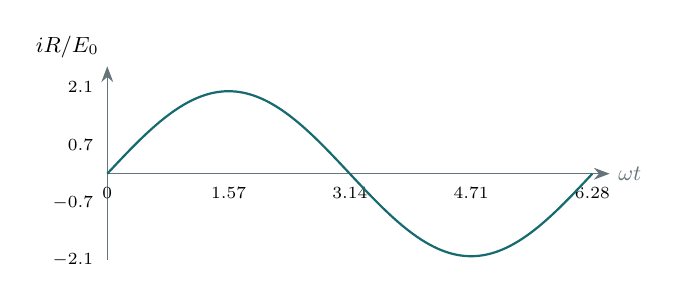
\begin{tikzpicture}[scale=.88,transform shape]
\draw[axis] (0,1.2500000)--(7.25,1.2500000) node[right] {$\omega t$};
\draw[axis] (0.0000000,0)--(0.0000000,2.8);
\node[above left] at (0.0000000,2.8) {$iR/E_0$};
\node[below,font=\scriptsize] at (0.0000000,1.1700000) {$0$};
\node[below,font=\scriptsize] at (1.7500000,1.1700000) {$1.57$};
\node[below,font=\scriptsize] at (3.5000000,1.1700000) {$3.14$};
\node[below,font=\scriptsize] at (5.2500000,1.1700000) {$4.71$};
\node[below,font=\scriptsize] at (7.0000000,1.1700000) {$6.28$};
\node[left,font=\scriptsize] at (-0.0800000,0.0000000) {$-2.1$};
\node[left,font=\scriptsize] at (-0.0800000,0.8333333) {$-0.7$};
\node[left,font=\scriptsize] at (-0.0800000,1.6666667) {$0.7$};
\node[left,font=\scriptsize] at (-0.0800000,2.5000000) {$2.1$};
\draw[thick,color=accent] plot coordinates {(0.0000000,1.2500000) (0.0291667,1.2811630) (0.0583333,1.3123047) (0.0875000,1.3434037) (0.1166667,1.3744386) (0.1458333,1.4053883) (0.1750000,1.4362315) (0.2041667,1.4669471) (0.2333333,1.4975139) (0.2625000,1.5279111) (0.2916667,1.5581179) (0.3208333,1.5881135) (0.3500000,1.6178774) (0.3791667,1.6473891) (0.4083333,1.6766285) (0.4375000,1.7055755) (0.4666667,1.7342103) (0.4958333,1.7625132) (0.5250000,1.7904649) (0.5541667,1.8180461) (0.5833333,1.8452381) (0.6125000,1.8720221) (0.6416667,1.8983798) (0.6708333,1.9242931) (0.7000000,1.9497443) (0.7291667,1.9747160) (0.7583333,1.9991909) (0.7875000,2.0231524) (0.8166667,2.0465841) (0.8458333,2.0694697) (0.8750000,2.0917938) (0.9041667,2.1135409) (0.9333333,2.1346962) (0.9625000,2.1552452) (0.9916667,2.1751738) (1.0208333,2.1944683) (1.0500000,2.2131155) (1.0791667,2.2311026) (1.1083333,2.2484173) (1.1375000,2.2650478) (1.1666667,2.2809826) (1.1958333,2.2962108) (1.2250000,2.3107221) (1.2541667,2.3245063) (1.2833333,2.3375541) (1.3125000,2.3498566) (1.3416667,2.3614053) (1.3708333,2.3721923) (1.4000000,2.3822101) (1.4291667,2.3914521) (1.4583333,2.3999117) (1.4875000,2.4075832) (1.5166667,2.4144614) (1.5458333,2.4205416) (1.5750000,2.4258195) (1.6041667,2.4302915) (1.6333333,2.4339546) (1.6625000,2.4368063) (1.6916667,2.4388447) (1.7208333,2.4400682) (1.7500000,2.4404762) (1.7791667,2.4400682) (1.8083333,2.4388447) (1.8375000,2.4368063) (1.8666667,2.4339546) (1.8958333,2.4302915) (1.9250000,2.4258195) (1.9541667,2.4205416) (1.9833333,2.4144614) (2.0125000,2.4075832) (2.0416667,2.3999117) (2.0708333,2.3914521) (2.1000000,2.3822101) (2.1291667,2.3721923) (2.1583333,2.3614053) (2.1875000,2.3498566) (2.2166667,2.3375541) (2.2458333,2.3245063) (2.2750000,2.3107221) (2.3041667,2.2962108) (2.3333333,2.2809826) (2.3625000,2.2650478) (2.3916667,2.2484173) (2.4208333,2.2311026) (2.4500000,2.2131155) (2.4791667,2.1944683) (2.5083333,2.1751738) (2.5375000,2.1552452) (2.5666667,2.1346962) (2.5958333,2.1135409) (2.6250000,2.0917938) (2.6541667,2.0694697) (2.6833333,2.0465841) (2.7125000,2.0231524) (2.7416667,1.9991909) (2.7708333,1.9747160) (2.8000000,1.9497443) (2.8291667,1.9242931) (2.8583333,1.8983798) (2.8875000,1.8720221) (2.9166667,1.8452381) (2.9458333,1.8180461) (2.9750000,1.7904649) (3.0041667,1.7625132) (3.0333333,1.7342103) (3.0625000,1.7055755) (3.0916667,1.6766285) (3.1208333,1.6473891) (3.1500000,1.6178774) (3.1791667,1.5881135) (3.2083333,1.5581179) (3.2375000,1.5279111) (3.2666667,1.4975139) (3.2958333,1.4669471) (3.3250000,1.4362315) (3.3541667,1.4053883) (3.3833333,1.3744386) (3.4125000,1.3434037) (3.4416667,1.3123047) (3.4708333,1.2811630) (3.5000000,1.2500000) (3.5291667,1.2188370) (3.5583333,1.1876953) (3.5875000,1.1565963) (3.6166667,1.1255614) (3.6458333,1.0946117) (3.6750000,1.0637685) (3.7041667,1.0330529) (3.7333333,1.0024861) (3.7625000,0.9720889) (3.7916667,0.9418821) (3.8208333,0.9118865) (3.8500000,0.8821226) (3.8791667,0.8526109) (3.9083333,0.8233715) (3.9375000,0.7944245) (3.9666667,0.7657897) (3.9958333,0.7374868) (4.0250000,0.7095351) (4.0541667,0.6819539) (4.0833333,0.6547619) (4.1125000,0.6279779) (4.1416667,0.6016202) (4.1708333,0.5757069) (4.2000000,0.5502557) (4.2291667,0.5252840) (4.2583333,0.5008091) (4.2875000,0.4768476) (4.3166667,0.4534159) (4.3458333,0.4305303) (4.3750000,0.4082062) (4.4041667,0.3864591) (4.4333333,0.3653038) (4.4625000,0.3447548) (4.4916667,0.3248262) (4.5208333,0.3055317) (4.5500000,0.2868845) (4.5791667,0.2688974) (4.6083333,0.2515827) (4.6375000,0.2349522) (4.6666667,0.2190174) (4.6958333,0.2037892) (4.7250000,0.1892779) (4.7541667,0.1754937) (4.7833333,0.1624459) (4.8125000,0.1501434) (4.8416667,0.1385947) (4.8708333,0.1278077) (4.9000000,0.1177899) (4.9291667,0.1085479) (4.9583333,0.1000883) (4.9875000,0.0924168) (5.0166667,0.0855386) (5.0458333,0.0794584) (5.0750000,0.0741805) (5.1041667,0.0697085) (5.1333333,0.0660454) (5.1625000,0.0631937) (5.1916667,0.0611553) (5.2208333,0.0599318) (5.2500000,0.0595238) (5.2791667,0.0599318) (5.3083333,0.0611553) (5.3375000,0.0631937) (5.3666667,0.0660454) (5.3958333,0.0697085) (5.4250000,0.0741805) (5.4541667,0.0794584) (5.4833333,0.0855386) (5.5125000,0.0924168) (5.5416667,0.1000883) (5.5708333,0.1085479) (5.6000000,0.1177899) (5.6291667,0.1278077) (5.6583333,0.1385947) (5.6875000,0.1501434) (5.7166667,0.1624459) (5.7458333,0.1754937) (5.7750000,0.1892779) (5.8041667,0.2037892) (5.8333333,0.2190174) (5.8625000,0.2349522) (5.8916667,0.2515827) (5.9208333,0.2688974) (5.9500000,0.2868845) (5.9791667,0.3055317) (6.0083333,0.3248262) (6.0375000,0.3447548) (6.0666667,0.3653038) (6.0958333,0.3864591) (6.1250000,0.4082062) (6.1541667,0.4305303) (6.1833333,0.4534159) (6.2125000,0.4768476) (6.2416667,0.5008091) (6.2708333,0.5252840) (6.3000000,0.5502557) (6.3291667,0.5757069) (6.3583333,0.6016202) (6.3875000,0.6279779) (6.4166667,0.6547619) (6.4458333,0.6819539) (6.4750000,0.7095351) (6.5041667,0.7374868) (6.5333333,0.7657897) (6.5625000,0.7944245) (6.5916667,0.8233715) (6.6208333,0.8526109) (6.6500000,0.8821226) (6.6791667,0.9118865) (6.7083333,0.9418821) (6.7375000,0.9720889) (6.7666667,1.0024861) (6.7958333,1.0330529) (6.8250000,1.0637685) (6.8541667,1.0946117) (6.8833333,1.1255614) (6.9125000,1.1565963) (6.9416667,1.1876953) (6.9708333,1.2188370) (7.0000000,1.2500000)};
\end{tikzpicture}
\figcaption{变式图综一.4V5\quad 同频且两支路电源反相时的电阻电流。}
\end{minipage}\end{center}
\item 仅左电源工作，连续改变其频率$\Omega$，其峰值仍为$E_0$。令$x=\Omega/\omega$，则$Z_L=\mathrm jRx$、$Z_C=-\mathrm jR/x$，从图A的串并联关系得
\[
\frac{RI_1}{E_1}=\frac{1-x^2}{1-x^2+\mathrm jx},\quad
\frac{R|I_1|}{E_0}=\frac{|1-x^2|}{\sqrt{(1-x^2)^2+x^2}}.
\]
$x=1$时电感与电容向下的电流等大反向，节点电势跟随左电源，电阻两端等势，电阻电流为零。图V6由低频下降到这一零点，随后随频率升高重新增大；$x\to0$及$x\to\infty$的幅值均趋于$E_0/R$，分别对应电感或电容提供低阻抗返回路径。
\begin{center}\begin{minipage}{.98\linewidth}\centering
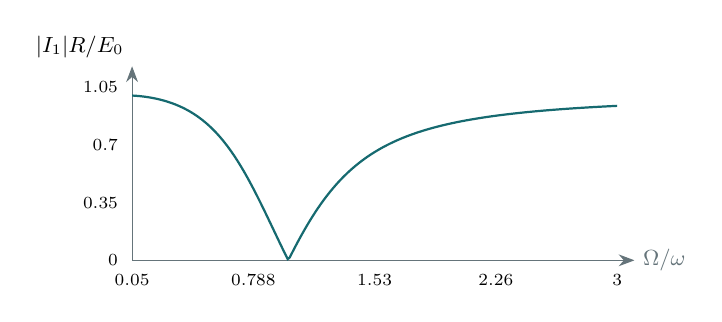
\begin{tikzpicture}[scale=.88,transform shape]
\draw[axis] (0,0.0000000)--(7.25,0.0000000) node[right] {$\Omega/\omega$};
\draw[axis] (0.0000000,0)--(0.0000000,2.8);
\node[above left] at (0.0000000,2.8) {$|I_1|R/E_0$};
\node[below,font=\scriptsize] at (0.0000000,-0.0800000) {$0.05$};
\node[below,font=\scriptsize] at (1.7500000,-0.0800000) {$0.788$};
\node[below,font=\scriptsize] at (3.5000000,-0.0800000) {$1.53$};
\node[below,font=\scriptsize] at (5.2500000,-0.0800000) {$2.26$};
\node[below,font=\scriptsize] at (7.0000000,-0.0800000) {$3$};
\node[left,font=\scriptsize] at (-0.0800000,0.0000000) {$0$};
\node[left,font=\scriptsize] at (-0.0800000,0.8333333) {$0.35$};
\node[left,font=\scriptsize] at (-0.0800000,1.6666667) {$0.7$};
\node[left,font=\scriptsize] at (-0.0800000,2.5000000) {$1.05$};
\draw[thick,color=accent] plot coordinates {(0.0000000,2.3779669) (0.0291667,2.3763106) (0.0583333,2.3742840) (0.0875000,2.3718825) (0.1166667,2.3691006) (0.1458333,2.3659321) (0.1750000,2.3623697) (0.2041667,2.3584055) (0.2333333,2.3540303) (0.2625000,2.3492345) (0.2916667,2.3440070) (0.3208333,2.3383361) (0.3500000,2.3322090) (0.3791667,2.3256119) (0.4083333,2.3185301) (0.4375000,2.3109476) (0.4666667,2.3028475) (0.4958333,2.2942119) (0.5250000,2.2850214) (0.5541667,2.2752560) (0.5833333,2.2648941) (0.6125000,2.2539133) (0.6416667,2.2422897) (0.6708333,2.2299985) (0.7000000,2.2170135) (0.7291667,2.2033076) (0.7583333,2.1888522) (0.7875000,2.1736180) (0.8166667,2.1575742) (0.8458333,2.1406893) (0.8750000,2.1229306) (0.9041667,2.1042644) (0.9333333,2.0846566) (0.9625000,2.0640720) (0.9916667,2.0424751) (1.0208333,2.0198297) (1.0500000,1.9960998) (1.0791667,1.9712489) (1.1083333,1.9452411) (1.1375000,1.9180410) (1.1666667,1.8896137) (1.1958333,1.8599257) (1.2250000,1.8289448) (1.2541667,1.7966410) (1.2833333,1.7629863) (1.3125000,1.7279555) (1.3416667,1.6915268) (1.3708333,1.6536821) (1.4000000,1.6144074) (1.4291667,1.5736936) (1.4583333,1.5315368) (1.4875000,1.4879388) (1.5166667,1.4429078) (1.5458333,1.3964585) (1.5750000,1.3486127) (1.6041667,1.2993997) (1.6333333,1.2488564) (1.6625000,1.1970273) (1.6916667,1.1439652) (1.7208333,1.0897303) (1.7500000,1.0343909) (1.7791667,0.9780226) (1.8083333,0.9207079) (1.8375000,0.8625360) (1.8666667,0.8036022) (1.8958333,0.7440067) (1.9250000,0.6838542) (1.9541667,0.6232529) (1.9833333,0.5623136) (2.0125000,0.5011486) (2.0416667,0.4398706) (2.0708333,0.3785920) (2.1000000,0.3174236) (2.1291667,0.2564737) (2.1583333,0.1958475) (2.1875000,0.1356458) (2.2166667,0.0759646) (2.2458333,0.0168946) (2.2750000,0.0414797) (2.3041667,0.0990801) (2.3333333,0.1558351) (2.3625000,0.2116803) (2.3916667,0.2665580) (2.4208333,0.3204176) (2.4500000,0.3732155) (2.4791667,0.4249146) (2.5083333,0.4754846) (2.5375000,0.5249010) (2.5666667,0.5731457) (2.5958333,0.6202058) (2.6250000,0.6660735) (2.6541667,0.7107461) (2.6833333,0.7542248) (2.7125000,0.7965151) (2.7416667,0.8376259) (2.7708333,0.8775692) (2.8000000,0.9163598) (2.8291667,0.9540151) (2.8583333,0.9905544) (2.8875000,1.0259988) (2.9166667,1.0603710) (2.9458333,1.0936948) (2.9750000,1.1259949) (3.0041667,1.1572971) (3.0333333,1.1876272) (3.0625000,1.2170120) (3.0916667,1.2454779) (3.1208333,1.2730518) (3.1500000,1.2997603) (3.1791667,1.3256299) (3.2083333,1.3506870) (3.2375000,1.3749573) (3.2666667,1.3984664) (3.2958333,1.4212392) (3.3250000,1.4433004) (3.3541667,1.4646738) (3.3833333,1.4853828) (3.4125000,1.5054501) (3.4416667,1.5248979) (3.4708333,1.5437477) (3.5000000,1.5620203) (3.5291667,1.5797359) (3.5583333,1.5969141) (3.5875000,1.6135738) (3.6166667,1.6297333) (3.6458333,1.6454102) (3.6750000,1.6606217) (3.7041667,1.6753841) (3.7333333,1.6897132) (3.7625000,1.7036245) (3.7916667,1.7171325) (3.8208333,1.7302516) (3.8500000,1.7429952) (3.8791667,1.7553767) (3.9083333,1.7674086) (3.9375000,1.7791030) (3.9666667,1.7904718) (3.9958333,1.8015262) (4.0250000,1.8122769) (4.0541667,1.8227344) (4.0833333,1.8329088) (4.1125000,1.8428096) (4.1416667,1.8524462) (4.1708333,1.8618274) (4.2000000,1.8709618) (4.2291667,1.8798576) (4.2583333,1.8885227) (4.2875000,1.8969649) (4.3166667,1.9051914) (4.3458333,1.9132092) (4.3750000,1.9210251) (4.4041667,1.9286458) (4.4333333,1.9360774) (4.4625000,1.9433259) (4.4916667,1.9503973) (4.5208333,1.9572971) (4.5500000,1.9640307) (4.5791667,1.9706032) (4.6083333,1.9770198) (4.6375000,1.9832851) (4.6666667,1.9894039) (4.6958333,1.9953806) (4.7250000,2.0012195) (4.7541667,2.0069248) (4.7833333,2.0125004) (4.8125000,2.0179503) (4.8416667,2.0232780) (4.8708333,2.0284873) (4.9000000,2.0335816) (4.9291667,2.0385642) (4.9583333,2.0434384) (4.9875000,2.0482072) (5.0166667,2.0528736) (5.0458333,2.0574406) (5.0750000,2.0619109) (5.1041667,2.0662873) (5.1333333,2.0705723) (5.1625000,2.0747685) (5.1916667,2.0788783) (5.2208333,2.0829041) (5.2500000,2.0868481) (5.2791667,2.0907126) (5.3083333,2.0944997) (5.3375000,2.0982114) (5.3666667,2.1018497) (5.3958333,2.1054166) (5.4250000,2.1089139) (5.4541667,2.1123435) (5.4833333,2.1157070) (5.5125000,2.1190062) (5.5416667,2.1222427) (5.5708333,2.1254181) (5.6000000,2.1285339) (5.6291667,2.1315916) (5.6583333,2.1345928) (5.6875000,2.1375387) (5.7166667,2.1404307) (5.7458333,2.1432702) (5.7750000,2.1460584) (5.8041667,2.1487966) (5.8333333,2.1514859) (5.8625000,2.1541276) (5.8916667,2.1567227) (5.9208333,2.1592724) (5.9500000,2.1617777) (5.9791667,2.1642396) (6.0083333,2.1666592) (6.0375000,2.1690375) (6.0666667,2.1713753) (6.0958333,2.1736737) (6.1250000,2.1759335) (6.1541667,2.1781555) (6.1833333,2.1803406) (6.2125000,2.1824897) (6.2416667,2.1846036) (6.2708333,2.1866829) (6.3000000,2.1887285) (6.3291667,2.1907412) (6.3583333,2.1927215) (6.3875000,2.1946703) (6.4166667,2.1965881) (6.4458333,2.1984758) (6.4750000,2.2003338) (6.5041667,2.2021628) (6.5333333,2.2039635) (6.5625000,2.2057363) (6.5916667,2.2074820) (6.6208333,2.2092010) (6.6500000,2.2108940) (6.6791667,2.2125614) (6.7083333,2.2142037) (6.7375000,2.2158215) (6.7666667,2.2174153) (6.7958333,2.2189855) (6.8250000,2.2205326) (6.8541667,2.2220571) (6.8833333,2.2235594) (6.9125000,2.2250399) (6.9416667,2.2264991) (6.9708333,2.2279374) (7.0000000,2.2293552)};
\end{tikzpicture}
\figcaption{变式图综一.4V6\quad 仅左电源工作时的电流频率响应。}
\end{minipage}\end{center}
\item 取两个单位幅度电流$\cos(\omega t/2)$、$\cos\omega t$，求从$t=0$开始、长为$T$的乘积平均。沿图V7的横坐标改变观察时长，积化和差后逐项积分得
\[
C(T)=\frac1T\int_0^T\cos(\omega t/2)\cos\omega t\,dt
=\frac12\left[\frac{\sin(\omega T/2)}{\omega T/2}+\frac{\sin(3\omega T/2)}{3\omega T/2}\right].
\]
$T\to0$时$C\to1$，与两电流的初值乘积相同；$T=4\pi/\omega$时两正弦都为零。若两分量峰值为$A,B$，交叉项对这一时间段平均电阻功率贡献$2RAB C(T)$。图上的正负区域说明短时加热可随起点和观察时长改变，完整共同周期则消去该项。
\begin{center}\begin{minipage}{.98\linewidth}\centering
\begin{tikzpicture}[scale=.88,transform shape]
\draw[axis] (0,0.5555556)--(7.25,0.5555556) node[right] {$\omega T$};
\draw[axis] (0.0000000,0)--(0.0000000,2.8);
\node[above left] at (0.0000000,2.8) {$\langle\cos(\omega t/2)\cos\omega t\rangle_T$};
\node[below,font=\scriptsize] at (0.0000000,0.4755556) {$0.05$};
\node[below,font=\scriptsize] at (1.7500000,0.4755556) {$3.18$};
\node[below,font=\scriptsize] at (3.5000000,0.4755556) {$6.31$};
\node[below,font=\scriptsize] at (5.2500000,0.4755556) {$9.44$};
\node[below,font=\scriptsize] at (7.0000000,0.4755556) {$12.6$};
\node[left,font=\scriptsize] at (-0.0800000,0.0000000) {$-0.3$};
\node[left,font=\scriptsize] at (-0.0800000,0.8333333) {$0.15$};
\node[left,font=\scriptsize] at (-0.0800000,1.6666667) {$0.6$};
\node[left,font=\scriptsize] at (-0.0800000,2.5000000) {$1.05$};
\draw[thick,color=accent] plot coordinates {(0.0000000,2.4064431) (0.0273438,2.4036382) (0.0546875,2.3990003) (0.0820312,2.3925430) (0.1093750,2.3842854) (0.1367188,2.3742516) (0.1640625,2.3624710) (0.1914062,2.3489780) (0.2187500,2.3338119) (0.2460938,2.3170168) (0.2734375,2.2986415) (0.3007812,2.2787390) (0.3281250,2.2573668) (0.3554687,2.2345862) (0.3828125,2.2104622) (0.4101562,2.1850637) (0.4375000,2.1584624) (0.4648438,2.1307334) (0.4921875,2.1019543) (0.5195312,2.0722051) (0.5468750,2.0415682) (0.5742188,2.0101276) (0.6015625,1.9779689) (0.6289062,1.9451789) (0.6562500,1.9118453) (0.6835938,1.8780564) (0.7109375,1.8439006) (0.7382812,1.8094666) (0.7656250,1.7748423) (0.7929688,1.7401152) (0.8203125,1.7053716) (0.8476562,1.6706966) (0.8750000,1.6361737) (0.9023438,1.6018845) (0.9296875,1.5679084) (0.9570313,1.5343224) (0.9843750,1.5012007) (1.0117188,1.4686147) (1.0390625,1.4366326) (1.0664062,1.4053191) (1.0937500,1.3747354) (1.1210938,1.3449390) (1.1484375,1.3159832) (1.1757813,1.2879175) (1.2031250,1.2607869) (1.2304688,1.2346324) (1.2578125,1.2094900) (1.2851563,1.1853918) (1.3125000,1.1623648) (1.3398437,1.1404317) (1.3671875,1.1196103) (1.3945312,1.0999139) (1.4218750,1.0813511) (1.4492188,1.0639259) (1.4765625,1.0476377) (1.5039062,1.0324815) (1.5312500,1.0184479) (1.5585937,1.0055230) (1.5859375,0.9936889) (1.6132812,0.9829238) (1.6406250,0.9732016) (1.6679688,0.9644929) (1.6953125,0.9567646) (1.7226562,0.9499801) (1.7500000,0.9441000) (1.7773437,0.9390816) (1.8046875,0.9348799) (1.8320312,0.9314470) (1.8593750,0.9287332) (1.8867188,0.9266865) (1.9140625,0.9252535) (1.9414062,0.9243789) (1.9687500,0.9240067) (1.9960938,0.9240796) (2.0234375,0.9245398) (2.0507812,0.9253291) (2.0781250,0.9263891) (2.1054688,0.9276615) (2.1328125,0.9290884) (2.1601562,0.9306126) (2.1875000,0.9321777) (2.2148438,0.9337284) (2.2421875,0.9352107) (2.2695312,0.9365723) (2.2968750,0.9377627) (2.3242188,0.9387331) (2.3515625,0.9394371) (2.3789062,0.9398307) (2.4062500,0.9398722) (2.4335938,0.9395228) (2.4609375,0.9387463) (2.4882812,0.9375096) (2.5156250,0.9357825) (2.5429688,0.9335381) (2.5703125,0.9307525) (2.5976563,0.9274052) (2.6250000,0.9234792) (2.6523437,0.9189604) (2.6796875,0.9138387) (2.7070312,0.9081068) (2.7343750,0.9017610) (2.7617188,0.8948011) (2.7890625,0.8872300) (2.8164062,0.8790538) (2.8437500,0.8702819) (2.8710937,0.8609267) (2.8984375,0.8510035) (2.9257812,0.8405307) (2.9531250,0.8295292) (2.9804688,0.8180225) (3.0078125,0.8060368) (3.0351562,0.7936004) (3.0625000,0.7807438) (3.0898437,0.7674994) (3.1171875,0.7539016) (3.1445312,0.7399861) (3.1718750,0.7257903) (3.1992188,0.7113528) (3.2265625,0.6967129) (3.2539062,0.6819110) (3.2812500,0.6669883) (3.3085937,0.6519860) (3.3359375,0.6369457) (3.3632812,0.6219092) (3.3906250,0.6069179) (3.4179688,0.5920129) (3.4453125,0.5772348) (3.4726562,0.5626233) (3.5000000,0.5482174) (3.5273438,0.5340549) (3.5546875,0.5201722) (3.5820313,0.5066044) (3.6093750,0.4933852) (3.6367188,0.4805464) (3.6640625,0.4681180) (3.6914062,0.4561280) (3.7187500,0.4446025) (3.7460938,0.4335652) (3.7734375,0.4230379) (3.8007813,0.4130398) (3.8281250,0.4035878) (3.8554688,0.3946964) (3.8828125,0.3863777) (3.9101562,0.3786411) (3.9375000,0.3714939) (3.9648438,0.3649404) (3.9921875,0.3589829) (4.0195312,0.3536208) (4.0468750,0.3488515) (4.0742188,0.3446697) (4.1015625,0.3410680) (4.1289062,0.3380365) (4.1562500,0.3355634) (4.1835938,0.3336347) (4.2109375,0.3322345) (4.2382812,0.3313448) (4.2656250,0.3309460) (4.2929688,0.3310170) (4.3203125,0.3315349) (4.3476562,0.3324756) (4.3750000,0.3338137) (4.4023438,0.3355228) (4.4296875,0.3375755) (4.4570313,0.3399434) (4.4843750,0.3425979) (4.5117188,0.3455094) (4.5390625,0.3486484) (4.5664062,0.3519850) (4.5937500,0.3554892) (4.6210937,0.3591312) (4.6484375,0.3628816) (4.6757812,0.3667112) (4.7031250,0.3705916) (4.7304688,0.3744947) (4.7578125,0.3783937) (4.7851562,0.3822624) (4.8125000,0.3860758) (4.8398438,0.3898101) (4.8671875,0.3934428) (4.8945312,0.3969525) (4.9218750,0.4003198) (4.9492188,0.4035264) (4.9765625,0.4065558) (5.0039062,0.4093933) (5.0312500,0.4120256) (5.0585938,0.4144415) (5.0859375,0.4166316) (5.1132812,0.4185881) (5.1406250,0.4203053) (5.1679688,0.4217793) (5.1953125,0.4230078) (5.2226562,0.4239908) (5.2500000,0.4247297) (5.2773438,0.4252278) (5.3046875,0.4254903) (5.3320312,0.4255239) (5.3593750,0.4253369) (5.3867188,0.4249393) (5.4140625,0.4243424) (5.4414062,0.4235591) (5.4687500,0.4226034) (5.4960938,0.4214908) (5.5234375,0.4202375) (5.5507812,0.4188610) (5.5781250,0.4173797) (5.6054687,0.4158126) (5.6328125,0.4141795) (5.6601563,0.4125008) (5.6875000,0.4107972) (5.7148438,0.4090896) (5.7421875,0.4073995) (5.7695312,0.4057480) (5.7968750,0.4041564) (5.8242188,0.4026456) (5.8515625,0.4012366) (5.8789062,0.3999495) (5.9062500,0.3988041) (5.9335938,0.3978197) (5.9609375,0.3970146) (5.9882812,0.3964063) (6.0156250,0.3960116) (6.0429688,0.3958459) (6.0703125,0.3959238) (6.0976563,0.3962585) (6.1250000,0.3968621) (6.1523438,0.3977453) (6.1796875,0.3989174) (6.2070312,0.4003863) (6.2343750,0.4021584) (6.2617188,0.4042387) (6.2890625,0.4066306) (6.3164062,0.4093360) (6.3437500,0.4123551) (6.3710938,0.4156869) (6.3984375,0.4193285) (6.4257812,0.4232757) (6.4531250,0.4275227) (6.4804688,0.4320624) (6.5078125,0.4368859) (6.5351563,0.4419834) (6.5625000,0.4473435) (6.5898438,0.4529535) (6.6171875,0.4587997) (6.6445313,0.4648671) (6.6718750,0.4711396) (6.6992188,0.4776005) (6.7265625,0.4842318) (6.7539062,0.4910148) (6.7812500,0.4979304) (6.8085938,0.5049585) (6.8359375,0.5120788) (6.8632812,0.5192704) (6.8906250,0.5265122) (6.9179688,0.5337830) (6.9453125,0.5410614) (6.9726563,0.5483260) (7.0000000,0.5555556)};
\end{tikzpicture}
\figcaption{变式图综一.4V7\quad 从零时刻开始的有限时长交叉项。}
\end{minipage}\end{center}
\item 在同频$\omega$下只保留两个内部电源，令$E_2=E_0$、$E_3=E_0e^{\mathrm j\delta}$，求相位差与平均功率的关系。由变式5的节点式得
\[
I=\frac{\mathrm jE_0}R(e^{\mathrm j\delta}-1),\quad
|I|=\frac{2E_0}R|\sin(\delta/2)|,\quad
\bar P=\frac{2E_0^2}R\sin^2(\delta/2).
\]
图V8的零点$\delta=0,2\pi$对应两源电势升高相同，上节点$V=0$，电阻两端等势；此时中、右支路中的电流仍可等大反向流动。$\delta=\pi$时两个驱动对电阻返回方向同向叠加，峰值为$2E_0/R$，平均功率达到$2E_0^2/R$。
\begin{center}\begin{minipage}{.98\linewidth}\centering
\begin{tikzpicture}[scale=.88,transform shape]
\draw[axis] (0,0.0000000)--(7.25,0.0000000) node[right] {$\delta$};
\draw[axis] (0.0000000,0)--(0.0000000,2.8);
\node[above left] at (0.0000000,2.8) {$|I|R/E_0$};
\node[below,font=\scriptsize] at (0.0000000,-0.0800000) {$0$};
\node[below,font=\scriptsize] at (1.7500000,-0.0800000) {$1.57$};
\node[below,font=\scriptsize] at (3.5000000,-0.0800000) {$3.14$};
\node[below,font=\scriptsize] at (5.2500000,-0.0800000) {$4.71$};
\node[below,font=\scriptsize] at (7.0000000,-0.0800000) {$6.28$};
\node[left,font=\scriptsize] at (-0.0800000,0.0000000) {$0$};
\node[left,font=\scriptsize] at (-0.0800000,0.8333333) {$0.7$};
\node[left,font=\scriptsize] at (-0.0800000,1.6666667) {$1.4$};
\node[left,font=\scriptsize] at (-0.0800000,2.5000000) {$2.1$};
\draw[thick,color=accent] plot coordinates {(0.0000000,0.0000000) (0.0291667,0.0311657) (0.0583333,0.0623261) (0.0875000,0.0934758) (0.1166667,0.1246094) (0.1458333,0.1557217) (0.1750000,0.1868074) (0.2041667,0.2178610) (0.2333333,0.2488773) (0.2625000,0.2798509) (0.2916667,0.3107766) (0.3208333,0.3416491) (0.3500000,0.3724630) (0.3791667,0.4032131) (0.4083333,0.4338941) (0.4375000,0.4645008) (0.4666667,0.4950278) (0.4958333,0.5254701) (0.5250000,0.5558223) (0.5541667,0.5860793) (0.5833333,0.6162358) (0.6125000,0.6462868) (0.6416667,0.6762270) (0.6708333,0.7060514) (0.7000000,0.7357547) (0.7291667,0.7653321) (0.7583333,0.7947782) (0.7875000,0.8240882) (0.8166667,0.8532570) (0.8458333,0.8822796) (0.8750000,0.9111510) (0.9041667,0.9398663) (0.9333333,0.9684206) (0.9625000,0.9968089) (0.9916667,1.0250264) (1.0208333,1.0530683) (1.0500000,1.0809298) (1.0791667,1.1086060) (1.1083333,1.1360923) (1.1375000,1.1633839) (1.1666667,1.1904762) (1.1958333,1.2173645) (1.2250000,1.2440442) (1.2541667,1.2705108) (1.2833333,1.2967596) (1.3125000,1.3227863) (1.3416667,1.3485863) (1.3708333,1.3741552) (1.4000000,1.3994887) (1.4291667,1.4245824) (1.4583333,1.4494320) (1.4875000,1.4740332) (1.5166667,1.4983819) (1.5458333,1.5224738) (1.5750000,1.5463049) (1.6041667,1.5698710) (1.6333333,1.5931681) (1.6625000,1.6161923) (1.6916667,1.6389395) (1.7208333,1.6614059) (1.7500000,1.6835876) (1.7791667,1.7054808) (1.8083333,1.7270818) (1.8375000,1.7483869) (1.8666667,1.7693924) (1.8958333,1.7900948) (1.9250000,1.8104904) (1.9541667,1.8305758) (1.9833333,1.8503475) (2.0125000,1.8698022) (2.0416667,1.8889365) (2.0708333,1.9077472) (2.1000000,1.9262309) (2.1291667,1.9443847) (2.1583333,1.9622052) (2.1875000,1.9796896) (2.2166667,1.9968347) (2.2458333,2.0136377) (2.2750000,2.0300956) (2.3041667,2.0462057) (2.3333333,2.0619652) (2.3625000,2.0773714) (2.3916667,2.0924217) (2.4208333,2.1071134) (2.4500000,2.1214441) (2.4791667,2.1354113) (2.5083333,2.1490126) (2.5375000,2.1622457) (2.5666667,2.1751082) (2.5958333,2.1875981) (2.6250000,2.1997132) (2.6541667,2.2114513) (2.6833333,2.2228105) (2.7125000,2.2337889) (2.7416667,2.2443845) (2.7708333,2.2545955) (2.8000000,2.2644203) (2.8291667,2.2738570) (2.8583333,2.2829041) (2.8875000,2.2915601) (2.9166667,2.2998234) (2.9458333,2.3076926) (2.9750000,2.3151665) (3.0041667,2.3222436) (3.0333333,2.3289229) (3.0625000,2.3352030) (3.0916667,2.3410831) (3.1208333,2.3465620) (3.1500000,2.3516389) (3.1791667,2.3563128) (3.2083333,2.3605830) (3.2375000,2.3644487) (3.2666667,2.3679093) (3.2958333,2.3709641) (3.3250000,2.3736127) (3.3541667,2.3758546) (3.3833333,2.3776894) (3.4125000,2.3791168) (3.4416667,2.3801365) (3.4708333,2.3807484) (3.5000000,2.3809524) (3.5291667,2.3807484) (3.5583333,2.3801365) (3.5875000,2.3791168) (3.6166667,2.3776894) (3.6458333,2.3758546) (3.6750000,2.3736127) (3.7041667,2.3709641) (3.7333333,2.3679093) (3.7625000,2.3644487) (3.7916667,2.3605830) (3.8208333,2.3563128) (3.8500000,2.3516389) (3.8791667,2.3465620) (3.9083333,2.3410831) (3.9375000,2.3352030) (3.9666667,2.3289229) (3.9958333,2.3222436) (4.0250000,2.3151665) (4.0541667,2.3076926) (4.0833333,2.2998234) (4.1125000,2.2915601) (4.1416667,2.2829041) (4.1708333,2.2738570) (4.2000000,2.2644203) (4.2291667,2.2545955) (4.2583333,2.2443845) (4.2875000,2.2337889) (4.3166667,2.2228105) (4.3458333,2.2114513) (4.3750000,2.1997132) (4.4041667,2.1875981) (4.4333333,2.1751082) (4.4625000,2.1622457) (4.4916667,2.1490126) (4.5208333,2.1354113) (4.5500000,2.1214441) (4.5791667,2.1071134) (4.6083333,2.0924217) (4.6375000,2.0773714) (4.6666667,2.0619652) (4.6958333,2.0462057) (4.7250000,2.0300956) (4.7541667,2.0136377) (4.7833333,1.9968347) (4.8125000,1.9796896) (4.8416667,1.9622052) (4.8708333,1.9443847) (4.9000000,1.9262309) (4.9291667,1.9077472) (4.9583333,1.8889365) (4.9875000,1.8698022) (5.0166667,1.8503475) (5.0458333,1.8305758) (5.0750000,1.8104904) (5.1041667,1.7900948) (5.1333333,1.7693924) (5.1625000,1.7483869) (5.1916667,1.7270818) (5.2208333,1.7054808) (5.2500000,1.6835876) (5.2791667,1.6614059) (5.3083333,1.6389395) (5.3375000,1.6161923) (5.3666667,1.5931681) (5.3958333,1.5698710) (5.4250000,1.5463049) (5.4541667,1.5224738) (5.4833333,1.4983819) (5.5125000,1.4740332) (5.5416667,1.4494320) (5.5708333,1.4245824) (5.6000000,1.3994887) (5.6291667,1.3741552) (5.6583333,1.3485863) (5.6875000,1.3227863) (5.7166667,1.2967596) (5.7458333,1.2705108) (5.7750000,1.2440442) (5.8041667,1.2173645) (5.8333333,1.1904762) (5.8625000,1.1633839) (5.8916667,1.1360923) (5.9208333,1.1086060) (5.9500000,1.0809298) (5.9791667,1.0530683) (6.0083333,1.0250264) (6.0375000,0.9968089) (6.0666667,0.9684206) (6.0958333,0.9398663) (6.1250000,0.9111510) (6.1541667,0.8822796) (6.1833333,0.8532570) (6.2125000,0.8240882) (6.2416667,0.7947782) (6.2708333,0.7653321) (6.3000000,0.7357547) (6.3291667,0.7060514) (6.3583333,0.6762270) (6.3875000,0.6462868) (6.4166667,0.6162358) (6.4458333,0.5860793) (6.4750000,0.5558223) (6.5041667,0.5254701) (6.5333333,0.4950278) (6.5625000,0.4645008) (6.5916667,0.4338941) (6.6208333,0.4032131) (6.6500000,0.3724630) (6.6791667,0.3416491) (6.7083333,0.3107766) (6.7375000,0.2798509) (6.7666667,0.2488773) (6.7958333,0.2178610) (6.8250000,0.1868074) (6.8541667,0.1557217) (6.8833333,0.1246094) (6.9125000,0.0934758) (6.9416667,0.0623261) (6.9708333,0.0311657) (7.0000000,0.0000000)};
\end{tikzpicture}
\figcaption{变式图综一.4V8\quad 两内部电源的相位差控制电阻电流峰值。}
\end{minipage}\end{center}
\end{enumerate}

\Needspace{13\baselineskip}

\pdfbookmark[2]{第 5 题 幂律径向电场中的粒子束聚焦}{q5}

\section*{第 5 题\quad 幂律径向电场中的粒子束聚焦}\label{q:5}


平面内有径向电场$\boldsymbol E=-\kappa r^{-\beta}\hat{\boldsymbol r}$，其中$\kappa>0$、$\beta\ne1$。质量$m$、正电荷$q$的粒子从$S$发射，不计粒子间作用、重力和辐射。
\begin{enumerate}
\item 粒子以切向速度$v_0$沿半径$r_0$的圆轨道运动，求$r_0$。
\item 发射速率均为$v_0$，方向相对圆轨道切线有小角度偏离：最外射线偏外$\alpha_{\rm out}$，最内射线偏内$\alpha_{\rm in}$，总角宽$\alpha=\alpha_{\rm out}+\alpha_{\rm in}\ll1$。求使粒子在距中心$r_0$处重新聚焦的$\beta$范围、第一次聚焦的方位角$\phi_1$，以及方位角$\phi_1/2$处的径向束宽。取$\beta=-13$，画出粒子从$S$到转过$2\pi$的轨迹示意。
\item 在上述可聚焦范围内，改为方向均沿切线，速率分布在$v_0$至$v_0+\Delta v$，其中$\Delta v/v_0\ll1$。求第一次聚焦角$\phi_2$及方位角$\phi_2/2$处径向束宽；同样画$\beta=-13$时的轨迹。
\end{enumerate}
聚焦位置和束宽均求小角度、小相对速度差的一阶近似，说明稳定性和近似条件。


\begin{center}\begin{minipage}{.98\linewidth}\centering
\begin{tikzpicture}[scale=.8,transform shape]

\draw[object] (0,0) circle (2.5);
\fill (0,0) circle (2pt) node[below left] {$O$};
\fill (2.5,0) circle (2pt) node[below right] {$S$};
\draw[guide] (0,0)--(2.5,0) node[midway,below] {$r_0$};
\draw[motion] (2.5,0)--(2.5,2) node[above] {$v_0$切向};
\draw[motion] (2.5,0)--(3.1,1.9);
\draw[motion] (2.5,0)--(1.9,1.9);
\draw[force] (1.77,1.77)--(.85,.85) node[midway,above left] {$q\boldsymbol E$};
\draw[axis] (.8,0) arc[start angle=0,end angle=55,radius=.8];
\node at (.95,.5) {$\theta$};
\node[align=left] at (6,.4) {（2）小角宽$\alpha$\\（3）切向速度展宽$\Delta v$\\$\boldsymbol E=-\kappa r^{-\beta}\hat{\boldsymbol r}$};

\end{tikzpicture}
\figcaption{图综一.5\quad 参考圆、径向电力与两种发射展宽条件。}
\end{minipage}\end{center}

\Needspace{8\baselineskip}

\pdfbookmark[3]{题型定位}{q5-h0}

\subsection*{题型定位}

稳定圆轨道附近的空间束流聚焦。方向展宽改变初始径向斜率，速度展宽同时改变角动量和径向平衡位置，因此方向束与速度束的首次聚焦角不同。

\Needspace{8\baselineskip}

\pdfbookmark[3]{知识点}{q5-h1}

\subsection*{知识点}

\begin{itemize}
\item 幂律中央电场、圆轨道条件和单位质量角动量。
\item 比耐方程、圆轨道一阶稳定性与径向振动。
\item 角度束的正弦扰动、速度束的常驱动余弦扰动。
\item 全束宽、聚焦方位角、空间交点与到达时间及二阶像差。
\end{itemize}

\Needspace{8\baselineskip}

\pdfbookmark[3]{物理图像}{q5-h2}

\subsection*{物理图像}

解图综一.5A标切线、径向方向及正负$\delta$。B在参考圆上画8个方向束焦点。C将速度扰动的平衡位置外移与振幅分开；D画四个速度束焦点。较快射线在这些位置接触参考圆，其余角度位于参考圆外侧。

\Needspace{8\baselineskip}

\pdfbookmark[3]{解题入口}{q5-h3}

\subsection*{解题入口}

先由圆轨道确定$r_0,h_0,u_0$。时间方程展开电场项与离心项，给出径向回复系数$3-\beta$；随后用比耐方程把轨迹统一写在相同方位角下。方向束的一阶角动量为$h_0$，初斜率由径向初速度给出；速度束展开$1/h^2$，由常驱动得到$1-\cos\eta\theta$。每问都从$r(\theta)$的共同交点求焦角，从极端射线的径向差求全束宽。

\Needspace{8\baselineskip}

\pdfbookmark[3]{标准解法}{q5-h4}

\subsection*{标准解法}


图综一.5的中心$O$指向发射点$S$，$OS=r_0$，参考粒子在$S$沿正方位角方向作切向运动。圆轨道条件为
\[
q\kappa r_0^{-\beta}=\frac{mv_0^2}{r_0},
\qquad
\boxed{r_0=\left(\frac{q\kappa}{mv_0^2}\right)^{1/(\beta-1)}}.
\]
题设取$\beta\ne1$，圆轨道条件据此唯一确定$r_0$。作为对照，$\beta=1$时同一条件变为$q\kappa=mv_0^2$，速度固定后，各半径均满足圆轨道条件。

圆轨道也是径向运动的参考平衡位置。对图中的切向发射稍作改变，粒子便在半径方向偏离参考圆。中央力对$O$的力矩为零，因此偏离过程中角动量守恒；半径增加时，角速度随之减小。径向恢复作用由电场力与角动量固定时的离心项共同决定，比较它们对半径的变化率，就能确定偏离是往复振动还是逐渐增大。方向展宽与速度展宽虽然都造成径向偏离，它们改变的初始量不同：前者在一阶内只给出径向初速度，后者还改变切向角动量，使每条射线的平衡位置外移。

令$\omega_0=v_0/r_0$，先把这一径向机制写成时间方程。对角动量为$h_0=r_0^2\omega_0$的粒子，置$r=r_0+x$，则
\[
\dot\theta=\frac{h_0}{r^2}
=\omega_0(1+x/r_0)^{-2}
=\omega_0(1-2x/r_0)+O(x^2/r_0^2).
\]
径向动力学方程$m\ddot r=mr\dot\theta^2-q\kappa r^{-\beta}$中的两项分别展开为
\[
\begin{aligned}
mr\dot\theta^2&=m\omega_0^2r_0(1+x/r_0)(1-4x/r_0)+O(x^2)
=m\omega_0^2r_0(1-3x/r_0)+O(x^2),\\
q\kappa r^{-\beta}&=q\kappa r_0^{-\beta}(1-\beta x/r_0)+O(x^2)
=m\omega_0^2r_0(1-\beta x/r_0)+O(x^2).
\end{aligned}
\]
常数项相消后，剩下
\[
\ddot x+(3-\beta)\omega_0^2x=0.
\]
其中$3$来自角动量守恒所决定的$h_0^2/r^3$项，$\beta$来自电场力随半径的变化。$\beta<3$时，向外偏离产生向内的合力，向内偏离产生向外的合力，径向运动为小振动。振动角频率与参考圆角速度之比为$\sqrt{3-\beta}$，它将直接决定轨迹在一周内交回参考圆的次数。

为把不同粒子的轨迹在同一方位角比较，使用比耐方程。比耐方程把时间换成方位角，可直接比较图上同一径向线穿过的多条射线。由$u=1/r$、$\dot\theta=hu^2$得
\[
\dot r=-hu',\qquad
\ddot r=-h^2u^2u'',\qquad
r\dot\theta^2=h^2u^3.
\]
将它们代入$\ddot r-r\dot\theta^2=-(q\kappa/m)r^{-\beta}$，除以$-h^2u^2$，便得到下面的轨道方程。因而这一步使用的仍是前述径向动力学和角动量守恒，只是把聚焦位置直接写成$\theta$的函数。
记单位质量角动量$h=r^2\dot\theta$、$u=1/r$，中央加速度为$-(q\kappa/m)r^{-\beta}$，于是
\[
u''+u=\frac{q\kappa}{mh^2}u^{\beta-2},
\]
撇号表示对$\theta$求导。圆轨道有$u_0=1/r_0$、$h_0=r_0v_0$，且
$(q\kappa/mh_0^2)u_0^{\beta-2}=u_0$。
\begin{center}\begin{minipage}{.98\linewidth}\centering
\begin{tikzpicture}[scale=.8,transform shape]

\draw[object] (0,0) circle (2.5);
\draw[guide] (2.5,-.8)--(2.5,3);
\draw[guide] (0,0)--(4,0) node[right] {径向外};
\fill (0,0) circle (2pt) node[below] {$O$};
\fill (2.5,0) circle (2pt) node[below right] {$S$};
\draw[motion] (2.5,0)--(3.4,2.3) node[above] {$\delta=\alpha_{\rm out}$};
\draw[motion] (2.5,0)--(1.6,2.3) node[above left] {$\delta=-\alpha_{\rm in}$};
\node[right] at (2.55,1) {$\delta$};
\node[align=left] at (6,-1) {$h=h_0+O(\delta^2)$\\$\dot r(0)=v_0\delta$\\$r-r_0\propto\sin(\eta\theta)$};

\end{tikzpicture}
\figcaption{解图综一.5A\quad 方向展宽一阶保留径向初速度，切向角动量的一阶变化为零。}
\end{minipage}\end{center}
第（2）问，解图综一.5A中初射方向与切线夹角$\delta$，偏外为正，偏内为负。由于$\cos\delta=1+O(\delta^2)$，一阶内$h=h_0$，径向初速度则保留$v_0\delta$。这两个初始条件分别进入轨道方程的系数和初斜率。
令$u=u_0+\zeta$，对比耐方程线性展开：
\[
\zeta''+\zeta=(\beta-2)\zeta
\ \Longrightarrow\ 
\zeta''+(3-\beta)\zeta=0.
\]
初始$\zeta(0)=0$。又由$\dot r=-h u'$，
\[
\zeta'(0)=-\frac{v_0\delta}{h_0}=-u_0\delta.
\]
若$\beta<3$，记$\eta=\sqrt{3-\beta}>0$，得
\[
\zeta=-\frac{u_0\delta}{\eta}\sin\eta\theta,\qquad
\boxed{r(\theta)=r_0+\frac{r_0\delta}{\eta}\sin\eta\theta
+O(\delta^2)}.
\]
所以第一次所有小角射线重新到达$r=r_0$且同一方位角处，是
\[
\boxed{\phi_1=\frac{\pi}{\sqrt{3-\beta}}}.
\]
在$\theta=\phi_1/2$处，正弦为一，最外和最内射线的径向偏移分别为$r_0\alpha_{\rm out}/\eta$和$-r_0\alpha_{\rm in}/\eta$，径向全束宽
\[
\boxed{\Delta r_1=\frac{\alpha r_0}{\sqrt{3-\beta}}}.
\]
聚焦点按相同方位角比较各条空间轨迹。取带符号的初始偏角 $\delta$，比角动量 $h=r_0v_0\cos\delta=r_0v_0+O(\delta^2)$。用解图综一.5B 中 $r/r_0=1+(\delta/4)\sin4\theta$ 的一阶轨迹，记 $\omega_0=v_0/r_0$，得到
\[
\frac{\mathrm dt}{\mathrm d\theta}=\frac{r^2}{h}
=\frac{1}{\omega_0}\left(1+\frac{\delta}{2}\sin4\theta\right)+O(\delta^2/\omega_0).
\]
从发射角 $0$ 积到 $\theta$，一阶到达时间比参考圆上的 $\theta/\omega_0$ 多 $\delta(1-\cos4\theta)/(8\omega_0)$。在奇数倍 $\pi/4$ 的焦点，正负偏角粒子经过同一地点，时间差是一阶量；在偶数倍 $\pi/4$ 的焦点，一阶时间差为零。

若$\beta=3$，扰动方程为$\zeta''=0$，非零初斜率引起线性漂移；若$\beta>3$，其解含$\sinh(\sqrt{\beta-3}\theta)$，也不重新为零。因此在题设$\beta\ne1$下，可聚焦范围为
\[
\boxed{\beta\in(-\infty,3)\setminus\{1\}}.
\]
等价的时间域径向小振动频率为
$\Omega_r=\sqrt{3-\beta}\,v_0/r_0$。靠近$\beta=3$时，径向恢复作用减弱，束宽中出现$1/\eta$放大因子；相应的小振动条件为$\alpha/\eta\ll1$，即展开后的$|r-r_0|/r_0$仍为小量。
\begin{center}\begin{minipage}{.98\linewidth}\centering
\begin{tikzpicture}[scale=.8,transform shape]

\draw[guide] (0,0) circle (3);
\foreach \a in {-.24,-.12,.12,.24}{
\draw[traj,domain=0:360,samples=361] plot ({(3+\a*sin(4*\x))*cos(\x)},{(3+\a*sin(4*\x))*sin(\x)});
}
\foreach \ang in {0,45,...,315}{\fill (\ang:3) circle (2pt);}
\fill (0,0) circle (2pt) node[below] {$O$};
\node[right] at (3.2,0) {$S$};
\node[above] at (0,3.3) {$\beta=-13,\quad\eta=4$};
\node at (0,-4) {每隔$\pi/4$交参考圆；径向偏移放大};

\end{tikzpicture}
\figcaption{解图综一.5B\quad 方向束的一阶轨迹，包含S在内的8个位置每周重复聚焦。}
\end{minipage}\end{center}
解图综一.5B取$\beta=-13$，$\eta=4$，轨迹一阶为
$r=r_0+(r_0\delta/4)\sin4\theta$。因此每隔$\pi/4$在参考圆上有一个聚焦点，离开$S$后，在$0<\theta\le2\pi$内共发生8次再聚焦，第8次回到$S$。内、外偏转两族在各焦点前后交换径向次序。

第（3）问改用切向速度$v=v_0(1+\epsilon)$发射，其中$\epsilon=(v-v_0)/v_0$。从时间域也能看清图C中平衡位置移动的大小。速度提高后$h=r_0v_0(1+\epsilon)$，径向方程中的离心项增加，而电场在出发点保持原值。一阶展开给出
\[
\begin{aligned}
\ddot x&=\frac{v_0^2}{r_0}(1+2\epsilon)(1-3x/r_0)
-\frac{v_0^2}{r_0}(1-\beta x/r_0)\\
&=2\epsilon\omega_0^2r_0-(3-\beta)\omega_0^2x.
\end{aligned}
\]
以$\eta^2=3-\beta$记回复系数，恒定驱动使平衡位置变为$x_{\rm eq}=2r_0\epsilon/\eta^2$。令$X=x-x_{\rm eq}$，则$\ddot X+\eta^2\omega_0^2X=0$。粒子从$r_0$切向射出，故$x(0)=\dot x(0)=0$，即$X(0)=-x_{\rm eq}$、$\dot X(0)=0$，振幅恰为$x_{\rm eq}$。沿图C从左到右，四分之一振动周期到平衡位置，半周期到最外侧$r_0+2x_{\rm eq}$，一整周期回到$r_0$。不同速度对应不同$x_{\rm eq}$，而一阶振动频率相同，因此第一次共同回到出发半径发生在整周期之后。

方向束则从$x=0$出发，初始径向速度分别为$v_0\alpha_{\rm out}$与$-v_0\alpha_{\rm in}$。其两侧振幅分别为$v_0\alpha_{\rm out}/\Omega_r$和$v_0\alpha_{\rm in}/\Omega_r$，所以半程的全束宽取两振幅之和。这个几何意义解释了$\alpha=\alpha_{\rm out}+\alpha_{\rm in}$进入结果的方式，切线在发散角内的偏置由两侧各自承担。

第（3）问，用$\epsilon=(v-v_0)/v_0\in[0,\Delta v/v_0]$。初始径向速度为零，但角动量已改变：
\[
h=h_0(1+\epsilon),\qquad
\frac1{h^2}=\frac1{h_0^2}(1-2\epsilon)+O(\epsilon^2).
\]
将$u=u_0+\zeta$和此式同时代入比耐方程，保留一阶项：
\[
\zeta''+(3-\beta)\zeta=-2u_0\epsilon,
\qquad \zeta(0)=\zeta'(0)=0.
\]
解为
\[
\zeta=-\frac{2u_0\epsilon}{\eta^2}(1-\cos\eta\theta),
\]
从而
\[
\boxed{r(\theta)=r_0+
\frac{2r_0\epsilon}{3-\beta}
[1-\cos(\sqrt{3-\beta}\theta)]+O(\epsilon^2)}.
\]
\begin{center}\begin{minipage}{.98\linewidth}\centering
\begin{tikzpicture}[scale=.8,transform shape]

\draw[axis] (0,0)--(8,0) node[right] {$\theta$};
\draw[axis] (0,0)--(0,4) node[above] {$r-r_0$};
\draw[guide] (0,1.5)--(7.2,1.5) node[right] {$x_{\rm eq}$};
\draw[traj,domain=0:360,samples=160] plot ({\x/50},{1.5*(1-cos(\x))});
\draw[guide] (3.6,0)--(3.6,3);
\node[below] at (3.6,0) {$\pi/\eta$};
\node[below] at (7.2,0) {$2\pi/\eta$};
\draw[axis,<->] (4.2,0)--(4.2,3);
\node[above] at (4.2,3.15) {$2x_{\rm eq}$};
\node at (3.8,4.7) {速度展宽：平衡位置外移，完整振动后回到$r_0$};

\end{tikzpicture}
\figcaption{解图综一.5C\quad 单条较快射线的径向偏移；最快粒子的$2x_{\rm eq}$即半程全束宽。}
\end{minipage}\end{center}
解图综一.5C画出恒定偏移和平移后的振动。较快粒子先偏向外侧；它的小振动中心相对参考圆外移
$x_{\rm eq}=2r_0\epsilon/(3-\beta)$，各条射线围绕各自的$r_0+x_{\rm eq}$振动。
第一次不同速率粒子都回到$r_0$需要余弦重新等于一，故
\[
\boxed{\phi_2=\frac{2\pi}{\sqrt{3-\beta}}=2\phi_1}.
\]
在$\phi_2/2$处余弦为$-1$，最慢参考粒子仍在$r_0$，最快粒子达到最大外偏，径向全束宽
\[
\boxed{\Delta r_2=
\frac{4r_0}{3-\beta}\frac{\Delta v}{v_0}}.
\]
速度束的小振动条件为$\Delta v/[(3-\beta)v_0]\ll1$。上述展开对每个固定的$\beta$取小展宽。若场力随半径变化特别快，保证$(1+|\beta|)|x|/r_0\ll1$即可使幂律展开中的高阶项保持很小。
\begin{center}\begin{minipage}{.98\linewidth}\centering
\begin{tikzpicture}[scale=.8,transform shape]

\draw[guide] (0,0) circle (3);
\foreach \a in {.05,.10,.15}{
\draw[traj,domain=0:360,samples=361] plot ({(3+\a*(1-cos(4*\x)))*cos(\x)},{(3+\a*(1-cos(4*\x)))*sin(\x)});
}
\foreach \ang in {0,90,180,270}{\fill (\ang:3) circle (2.5pt);}
\fill (0,0) circle (2pt) node[below] {$O$};
\node[right] at (3.25,0) {$S$};
\node[above] at (0,3.5) {$\beta=-13,\quad\phi_2=\pi/2$};
\node at (0,-4.1) {较快射线均在圆外；径向偏移放大};

\end{tikzpicture}
\figcaption{解图综一.5D\quad 速度束的一阶轨迹，每隔$\pi/2$回到参考圆，一周4次。}
\end{minipage}\end{center}
解图综一.5D中$\beta=-13$，速度束轨迹为
\[
r=r_0+\frac{r_0\epsilon}{8}(1-\cos4\theta),
\quad
\phi_2=\frac\pi2,\quad
\Delta r_2=\frac{r_0\Delta v}{4v_0}.
\]
它们均在参考圆外侧或圆上，每隔$\pi/2$聚焦，一周4次；这与方向展宽的一周8次不同。上述图线保留偏角和相对速度差的一阶项。有限展宽的轨迹还含二阶项，焦点附近的实际束斑可由继续展开轨道方程求出；这里的聚焦角和束宽描述一阶聚焦。


\Needspace{8\baselineskip}

\pdfbookmark[3]{关键洞察}{q5-h5}

\subsection*{关键洞察}

方向束从同一径向平衡位置带着不同径向初速度出发，故半个径向周期后交回参考圆。速度束从各自振动的内侧极点出发，其平衡位置随速度外移，故一整周期后才共同回到参考圆。图B的正弦零点与图D的余弦取一位置，分别把这两种初始状态变为八个和四个焦点。

\Needspace{8\baselineskip}

\pdfbookmark[3]{易错点}{q5-h6}

\subsection*{易错点}

\begin{itemize}
\item 图A的切向速度$v_0\cos\delta$与$v_0$相差二阶，径向速度$v_0\sin\delta$却有一阶项。方向束的$h$取$h_0$，初始径向速度保留$v_0\delta$。
\item 速度束的$h=h_0(1+\epsilon)$使$1/h^2$出现$-2\epsilon$，这正是径向平衡位置外移的驱动项。
\item $\alpha$为两侧最大偏角之和；束宽用最外射线减最内射线，图A中的切线位置可以偏离发散范围的中线。
\item 聚焦角比较同一方位角的空间轨迹，到达时刻可由$dt=r^2d\theta/h$分别积分求得。
\item 接近$\beta=3$时，小量条件按实际径向偏移写为$\alpha/\eta\ll1$与$(\Delta v/v_0)/\eta^2\ll1$，它们随恢复作用减弱而收紧。
\end{itemize}

\Needspace{8\baselineskip}

\pdfbookmark[3]{课堂讲解建议}{q5-h7}

\subsection*{课堂讲解建议}

先让学生在图A上指出切向和径向，分别填写方向束、速度束的$r(0),\dot r(0),h$。追问：“方向偏转为何使$h$到二阶才变化？”回答是切向分量含$\cos\delta$；“径向分量是几阶？”回答是$\sin\delta=\delta+O(\delta^3)$。径向展开时保留电场和离心项两行，请学生分别指出离心项给出的$3$和电场项给出的$-\beta$。讲速度束前问：“较快粒子在S点的初始径向加速度向哪？”由$v^2/r_0-q\kappa r_0^{-\beta}/m>0$回答向外，再用图C解释振动中心与振幅都等于$x_{\rm eq}$。最后在$\beta=-13$的图B、D上数零点：方向束每隔$\pi/4$，速度束每隔$\pi/2$；问及原因时分别回答“过平衡位置”和“回到内侧极点”。

\Needspace{8\baselineskip}

\pdfbookmark[3]{变式训练}{q5-h8}

\subsection*{变式训练}

\begin{enumerate}
\item 取$\beta=2$，求两种聚焦角及半程宽度，并写出纯速度展宽的精确轨道。此时$\eta=1$，故$\phi_1=\pi$、$\Delta r_1=\alpha r_0$；$\phi_2=2\pi$、$\Delta r_2=4r_0\Delta v/v_0$。图V1中方向项的第一个零点在$\pi$，速度项到$2\pi$才回零。平方反比场的比耐方程右端为常数；对切向速度$v=v_0(1+\epsilon)$，初值$u(0)=u_0,u'(0)=0$给出
\[
\frac{u}{u_0}=\frac1{(1+\epsilon)^2}+\left[1-\frac1{(1+\epsilon)^2}\right]\cos\theta.
\]
在束内速度均小于$\sqrt2v_0$时各轨道为椭圆，$\theta=2\pi$恰回到S，纯速度束在此精确共点。将分母对$\epsilon$展开，得到$r/r_0=1+2\epsilon(1-\cos\theta)+O(\epsilon^2)$，图V1正是这一阶曲线。方向展宽的$h=h_0\cos\delta$还含二阶变化，其有限角宽束斑可由同一精确方程求得。
\begin{center}\begin{minipage}{.98\linewidth}\centering
\begin{tikzpicture}[scale=.88,transform shape]
\draw[axis] (0,0.8928571)--(7.25,0.8928571) node[right] {$\theta$};
\draw[axis] (0.0000000,0)--(0.0000000,2.8);
\node[above left] at (0.0000000,2.8) {$(r-r_0)/r_0$};
\node[below,font=\scriptsize] at (0.0000000,0.8128571) {$0$};
\node[below,font=\scriptsize] at (1.7500000,0.8128571) {$1.57$};
\node[below,font=\scriptsize] at (3.5000000,0.8128571) {$3.14$};
\node[below,font=\scriptsize] at (5.2500000,0.8128571) {$4.71$};
\node[below,font=\scriptsize] at (7.0000000,0.8128571) {$6.28$};
\node[left,font=\scriptsize] at (-0.0800000,0.0000000) {$-0.025$};
\node[left,font=\scriptsize] at (-0.0800000,0.8333333) {$-0.00167$};
\node[left,font=\scriptsize] at (-0.0800000,1.6666667) {$0.0217$};
\node[left,font=\scriptsize] at (-0.0800000,2.5000000) {$0.045$};
\draw[thick,color=accent] plot coordinates {(0.0000000,0.8928571) (0.0273438,0.9103866) (0.0546875,0.9279055) (0.0820312,0.9454033) (0.1093750,0.9628694) (0.1367188,0.9802933) (0.1640625,0.9976646) (0.1914062,1.0149728) (0.2187500,1.0322074) (0.2460938,1.0493580) (0.2734375,1.0664144) (0.3007812,1.0833663) (0.3281250,1.1002033) (0.3554688,1.1169155) (0.3828125,1.1334928) (0.4101562,1.1499250) (0.4375000,1.1662025) (0.4648438,1.1823152) (0.4921875,1.1982536) (0.5195312,1.2140081) (0.5468750,1.2295691) (0.5742188,1.2449273) (0.6015625,1.2600734) (0.6289062,1.2749983) (0.6562500,1.2896930) (0.6835938,1.3041487) (0.7109375,1.3183566) (0.7382812,1.3323083) (0.7656250,1.3459952) (0.7929688,1.3594092) (0.8203125,1.3725421) (0.8476562,1.3853861) (0.8750000,1.3979334) (0.9023438,1.4101765) (0.9296875,1.4221079) (0.9570312,1.4337206) (0.9843750,1.4450075) (1.0117188,1.4559617) (1.0390625,1.4665768) (1.0664062,1.4768463) (1.0937500,1.4867640) (1.1210937,1.4963240) (1.1484375,1.5055204) (1.1757812,1.5143479) (1.2031250,1.5228009) (1.2304688,1.5308745) (1.2578125,1.5385638) (1.2851562,1.5458641) (1.3125000,1.5527711) (1.3398437,1.5592806) (1.3671875,1.5653886) (1.3945312,1.5710916) (1.4218750,1.5763860) (1.4492188,1.5812686) (1.4765625,1.5857366) (1.5039063,1.5897872) (1.5312500,1.5934181) (1.5585938,1.5966269) (1.5859375,1.5994118) (1.6132812,1.6017711) (1.6406250,1.6037034) (1.6679688,1.6052075) (1.6953125,1.6062825) (1.7226563,1.6069277) (1.7500000,1.6071429) (1.7773437,1.6069277) (1.8046875,1.6062825) (1.8320312,1.6052075) (1.8593750,1.6037034) (1.8867188,1.6017711) (1.9140625,1.5994118) (1.9414062,1.5966269) (1.9687500,1.5934181) (1.9960937,1.5897872) (2.0234375,1.5857366) (2.0507812,1.5812686) (2.0781250,1.5763860) (2.1054688,1.5710916) (2.1328125,1.5653886) (2.1601562,1.5592806) (2.1875000,1.5527711) (2.2148438,1.5458641) (2.2421875,1.5385638) (2.2695312,1.5308745) (2.2968750,1.5228009) (2.3242188,1.5143479) (2.3515625,1.5055204) (2.3789062,1.4963240) (2.4062500,1.4867640) (2.4335938,1.4768463) (2.4609375,1.4665768) (2.4882812,1.4559617) (2.5156250,1.4450075) (2.5429687,1.4337206) (2.5703125,1.4221079) (2.5976562,1.4101765) (2.6250000,1.3979334) (2.6523437,1.3853861) (2.6796875,1.3725421) (2.7070313,1.3594092) (2.7343750,1.3459952) (2.7617188,1.3323083) (2.7890625,1.3183566) (2.8164062,1.3041487) (2.8437500,1.2896930) (2.8710938,1.2749983) (2.8984375,1.2600734) (2.9257812,1.2449273) (2.9531250,1.2295691) (2.9804687,1.2140081) (3.0078125,1.1982536) (3.0351563,1.1823152) (3.0625000,1.1662025) (3.0898438,1.1499250) (3.1171875,1.1334928) (3.1445313,1.1169155) (3.1718750,1.1002033) (3.1992188,1.0833663) (3.2265625,1.0664144) (3.2539062,1.0493580) (3.2812500,1.0322074) (3.3085938,1.0149728) (3.3359375,0.9976646) (3.3632812,0.9802933) (3.3906250,0.9628694) (3.4179688,0.9454033) (3.4453125,0.9279055) (3.4726562,0.9103866) (3.5000000,0.8928571) (3.5273438,0.8753277) (3.5546875,0.8578088) (3.5820312,0.8403110) (3.6093750,0.8228449) (3.6367188,0.8054209) (3.6640625,0.7880497) (3.6914062,0.7707415) (3.7187500,0.7535069) (3.7460938,0.7363563) (3.7734375,0.7192999) (3.8007812,0.7023480) (3.8281250,0.6855109) (3.8554687,0.6687988) (3.8828125,0.6522215) (3.9101562,0.6357893) (3.9375000,0.6195118) (3.9648437,0.6033991) (3.9921875,0.5874606) (4.0195312,0.5717062) (4.0468750,0.5561452) (4.0742188,0.5407870) (4.1015625,0.5256409) (4.1289062,0.5107160) (4.1562500,0.4960213) (4.1835938,0.4815656) (4.2109375,0.4673576) (4.2382812,0.4534060) (4.2656250,0.4397191) (4.2929688,0.4263051) (4.3203125,0.4131722) (4.3476562,0.4003282) (4.3750000,0.3877809) (4.4023438,0.3755378) (4.4296875,0.3636063) (4.4570312,0.3519937) (4.4843750,0.3407068) (4.5117187,0.3297526) (4.5390625,0.3191375) (4.5664062,0.3088680) (4.5937500,0.2989503) (4.6210938,0.2893903) (4.6484375,0.2801938) (4.6757812,0.2713664) (4.7031250,0.2629134) (4.7304688,0.2548398) (4.7578125,0.2471505) (4.7851562,0.2398502) (4.8125000,0.2329432) (4.8398438,0.2264337) (4.8671875,0.2203257) (4.8945312,0.2146227) (4.9218750,0.2093283) (4.9492188,0.2044457) (4.9765625,0.1999777) (5.0039062,0.1959270) (5.0312500,0.1922962) (5.0585937,0.1890874) (5.0859375,0.1863025) (5.1132813,0.1839432) (5.1406250,0.1820109) (5.1679688,0.1805068) (5.1953125,0.1794318) (5.2226562,0.1787866) (5.2500000,0.1785714) (5.2773438,0.1787866) (5.3046875,0.1794318) (5.3320312,0.1805068) (5.3593750,0.1820109) (5.3867188,0.1839432) (5.4140625,0.1863025) (5.4414062,0.1890874) (5.4687500,0.1922962) (5.4960938,0.1959270) (5.5234375,0.1999777) (5.5507812,0.2044457) (5.5781250,0.2093283) (5.6054687,0.2146227) (5.6328125,0.2203257) (5.6601562,0.2264337) (5.6875000,0.2329432) (5.7148438,0.2398502) (5.7421875,0.2471505) (5.7695313,0.2548398) (5.7968750,0.2629134) (5.8242188,0.2713664) (5.8515625,0.2801938) (5.8789062,0.2893903) (5.9062500,0.2989503) (5.9335938,0.3088680) (5.9609375,0.3191375) (5.9882813,0.3297526) (6.0156250,0.3407068) (6.0429688,0.3519937) (6.0703125,0.3636063) (6.0976562,0.3755378) (6.1250000,0.3877809) (6.1523438,0.4003282) (6.1796875,0.4131722) (6.2070312,0.4263051) (6.2343750,0.4397191) (6.2617187,0.4534060) (6.2890625,0.4673576) (6.3164063,0.4815656) (6.3437500,0.4960213) (6.3710938,0.5107160) (6.3984375,0.5256409) (6.4257812,0.5407870) (6.4531250,0.5561452) (6.4804688,0.5717062) (6.5078125,0.5874606) (6.5351562,0.6033991) (6.5625000,0.6195118) (6.5898438,0.6357893) (6.6171875,0.6522215) (6.6445312,0.6687988) (6.6718750,0.6855109) (6.6992188,0.7023480) (6.7265625,0.7192999) (6.7539062,0.7363563) (6.7812500,0.7535069) (6.8085937,0.7707415) (6.8359375,0.7880497) (6.8632812,0.8054209) (6.8906250,0.8228449) (6.9179688,0.8403110) (6.9453125,0.8578088) (6.9726563,0.8753277) (7.0000000,0.8928571)};
\draw[thick,color=accent] (7.65,2.4)--(8.1,2.4);\node[right,font=\scriptsize] at (8.15,2.4) {$\delta=0.02$};
\draw[thick,dashed,color=warm] plot coordinates {(0.0000000,0.8928571) (0.0273438,0.8930723) (0.0546875,0.8937175) (0.0820312,0.8947925) (0.1093750,0.8962966) (0.1367188,0.8982289) (0.1640625,0.9005882) (0.1914062,0.9033731) (0.2187500,0.9065819) (0.2460938,0.9102128) (0.2734375,0.9142634) (0.3007812,0.9187314) (0.3281250,0.9236140) (0.3554688,0.9289084) (0.3828125,0.9346114) (0.4101562,0.9407194) (0.4375000,0.9472289) (0.4648438,0.9541359) (0.4921875,0.9614362) (0.5195312,0.9691255) (0.5468750,0.9771991) (0.5742188,0.9856521) (0.6015625,0.9944796) (0.6289062,1.0036760) (0.6562500,1.0132360) (0.6835938,1.0231537) (0.7109375,1.0334232) (0.7382812,1.0440383) (0.7656250,1.0549925) (0.7929688,1.0662794) (0.8203125,1.0778921) (0.8476562,1.0898235) (0.8750000,1.1020666) (0.9023438,1.1146139) (0.9296875,1.1274579) (0.9570312,1.1405908) (0.9843750,1.1540048) (1.0117188,1.1676917) (1.0390625,1.1816434) (1.0664062,1.1958513) (1.0937500,1.2103070) (1.1210937,1.2250017) (1.1484375,1.2399266) (1.1757812,1.2550727) (1.2031250,1.2704309) (1.2304688,1.2859919) (1.2578125,1.3017464) (1.2851562,1.3176848) (1.3125000,1.3337975) (1.3398437,1.3500750) (1.3671875,1.3665072) (1.3945312,1.3830845) (1.4218750,1.3997967) (1.4492188,1.4166337) (1.4765625,1.4335856) (1.5039063,1.4506420) (1.5312500,1.4677926) (1.5585938,1.4850272) (1.5859375,1.5023354) (1.6132812,1.5197067) (1.6406250,1.5371306) (1.6679688,1.5545967) (1.6953125,1.5720945) (1.7226563,1.5896134) (1.7500000,1.6071429) (1.7773437,1.6246723) (1.8046875,1.6421912) (1.8320312,1.6596890) (1.8593750,1.6771551) (1.8867188,1.6945791) (1.9140625,1.7119503) (1.9414062,1.7292585) (1.9687500,1.7464931) (1.9960937,1.7636437) (2.0234375,1.7807001) (2.0507812,1.7976520) (2.0781250,1.8144891) (2.1054688,1.8312012) (2.1328125,1.8477785) (2.1601562,1.8642107) (2.1875000,1.8804882) (2.2148438,1.8966009) (2.2421875,1.9125394) (2.2695312,1.9282938) (2.2968750,1.9438548) (2.3242188,1.9592130) (2.3515625,1.9743591) (2.3789062,1.9892840) (2.4062500,2.0039787) (2.4335938,2.0184344) (2.4609375,2.0326424) (2.4882812,2.0465940) (2.5156250,2.0602809) (2.5429687,2.0736949) (2.5703125,2.0868278) (2.5976562,2.0996718) (2.6250000,2.1122191) (2.6523437,2.1244622) (2.6796875,2.1363937) (2.7070313,2.1480063) (2.7343750,2.1592932) (2.7617188,2.1702474) (2.7890625,2.1808625) (2.8164062,2.1911320) (2.8437500,2.2010497) (2.8710938,2.2106097) (2.8984375,2.2198062) (2.9257812,2.2286336) (2.9531250,2.2370866) (2.9804687,2.2451602) (3.0078125,2.2528495) (3.0351563,2.2601498) (3.0625000,2.2670568) (3.0898438,2.2735663) (3.1171875,2.2796743) (3.1445313,2.2853773) (3.1718750,2.2906717) (3.1992188,2.2955543) (3.2265625,2.3000223) (3.2539062,2.3040730) (3.2812500,2.3077038) (3.3085938,2.3109126) (3.3359375,2.3136975) (3.3632812,2.3160568) (3.3906250,2.3179891) (3.4179688,2.3194932) (3.4453125,2.3205682) (3.4726562,2.3212134) (3.5000000,2.3214286) (3.5273438,2.3212134) (3.5546875,2.3205682) (3.5820312,2.3194932) (3.6093750,2.3179891) (3.6367188,2.3160568) (3.6640625,2.3136975) (3.6914062,2.3109126) (3.7187500,2.3077038) (3.7460938,2.3040730) (3.7734375,2.3000223) (3.8007812,2.2955543) (3.8281250,2.2906717) (3.8554687,2.2853773) (3.8828125,2.2796743) (3.9101562,2.2735663) (3.9375000,2.2670568) (3.9648437,2.2601498) (3.9921875,2.2528495) (4.0195312,2.2451602) (4.0468750,2.2370866) (4.0742188,2.2286336) (4.1015625,2.2198062) (4.1289062,2.2106097) (4.1562500,2.2010497) (4.1835938,2.1911320) (4.2109375,2.1808625) (4.2382812,2.1702474) (4.2656250,2.1592932) (4.2929688,2.1480063) (4.3203125,2.1363937) (4.3476562,2.1244622) (4.3750000,2.1122191) (4.4023438,2.0996718) (4.4296875,2.0868278) (4.4570312,2.0736949) (4.4843750,2.0602809) (4.5117187,2.0465940) (4.5390625,2.0326424) (4.5664062,2.0184344) (4.5937500,2.0039787) (4.6210938,1.9892840) (4.6484375,1.9743591) (4.6757812,1.9592130) (4.7031250,1.9438548) (4.7304688,1.9282938) (4.7578125,1.9125394) (4.7851562,1.8966009) (4.8125000,1.8804882) (4.8398438,1.8642107) (4.8671875,1.8477785) (4.8945312,1.8312012) (4.9218750,1.8144891) (4.9492188,1.7976520) (4.9765625,1.7807001) (5.0039062,1.7636437) (5.0312500,1.7464931) (5.0585937,1.7292585) (5.0859375,1.7119503) (5.1132813,1.6945791) (5.1406250,1.6771551) (5.1679688,1.6596890) (5.1953125,1.6421912) (5.2226562,1.6246723) (5.2500000,1.6071429) (5.2773438,1.5896134) (5.3046875,1.5720945) (5.3320312,1.5545967) (5.3593750,1.5371306) (5.3867188,1.5197067) (5.4140625,1.5023354) (5.4414062,1.4850272) (5.4687500,1.4677926) (5.4960938,1.4506420) (5.5234375,1.4335856) (5.5507812,1.4166337) (5.5781250,1.3997967) (5.6054687,1.3830845) (5.6328125,1.3665072) (5.6601562,1.3500750) (5.6875000,1.3337975) (5.7148438,1.3176848) (5.7421875,1.3017464) (5.7695313,1.2859919) (5.7968750,1.2704309) (5.8242188,1.2550727) (5.8515625,1.2399266) (5.8789062,1.2250017) (5.9062500,1.2103070) (5.9335938,1.1958513) (5.9609375,1.1816434) (5.9882813,1.1676917) (6.0156250,1.1540048) (6.0429688,1.1405908) (6.0703125,1.1274579) (6.0976562,1.1146139) (6.1250000,1.1020666) (6.1523438,1.0898235) (6.1796875,1.0778921) (6.2070312,1.0662794) (6.2343750,1.0549925) (6.2617187,1.0440383) (6.2890625,1.0334232) (6.3164063,1.0231537) (6.3437500,1.0132360) (6.3710938,1.0036760) (6.3984375,0.9944796) (6.4257812,0.9856521) (6.4531250,0.9771991) (6.4804688,0.9691255) (6.5078125,0.9614362) (6.5351562,0.9541359) (6.5625000,0.9472289) (6.5898438,0.9407194) (6.6171875,0.9346114) (6.6445312,0.9289084) (6.6718750,0.9236140) (6.6992188,0.9187314) (6.7265625,0.9142634) (6.7539062,0.9102128) (6.7812500,0.9065819) (6.8085937,0.9033731) (6.8359375,0.9005882) (6.8632812,0.8982289) (6.8906250,0.8962966) (6.9179688,0.8947925) (6.9453125,0.8937175) (6.9726563,0.8930723) (7.0000000,0.8928571)};
\draw[thick,dashed,color=warm] (7.65,1.9)--(8.1,1.9);\node[right,font=\scriptsize] at (8.15,1.9) {$\epsilon=0.01$};
\end{tikzpicture}
\figcaption{变式图综一.5V1\quad 平方反比场中的方向扰动与速度扰动。}
\end{minipage}\end{center}
\item 取$\beta=-1$，角宽$\alpha=0.02$、速度宽$\Delta v/v_0=0.01$，求两个半程全束宽。$\eta=2$，于是$\phi_1=\pi/2$、$\phi_2=\pi$，并且
\[
\Delta r_1=\frac{0.02r_0}{2}=0.01r_0,\qquad
\Delta r_2=\frac{4r_0(0.01)}4=0.01r_0.
\]
图V2取对称方向束的外侧极端射线$\delta=0.01$，其最大偏移为$0.005r_0$，内侧极端射线给出相反偏移；速度束则由参考圆到最大外偏$0.01r_0$组成。两种全束宽相同，焦角分别对应半个与整个径向振动周期。此场的笛卡尔方程为$\ddot{\boldsymbol r}=-\omega_0^2\boldsymbol r$，切向速度束有$X=r_0\cos\omega_0t$、$Y=r_0(1+\epsilon)\sin\omega_0t$，在$t=\pi/\omega_0$各自精确到达$(-r_0,0)$，与$\phi_2=\pi$相符。
\begin{center}\begin{minipage}{.98\linewidth}\centering
\begin{tikzpicture}[scale=.88,transform shape]
\draw[axis] (0,0.8823529)--(7.25,0.8823529) node[right] {$\theta$};
\draw[axis] (0.0000000,0)--(0.0000000,2.8);
\node[above left] at (0.0000000,2.8) {$(r-r_0)/r_0$};
\node[below,font=\scriptsize] at (0.0000000,0.8023529) {$0$};
\node[below,font=\scriptsize] at (1.7500000,0.8023529) {$1.57$};
\node[below,font=\scriptsize] at (3.5000000,0.8023529) {$3.14$};
\node[below,font=\scriptsize] at (5.2500000,0.8023529) {$4.71$};
\node[below,font=\scriptsize] at (7.0000000,0.8023529) {$6.28$};
\node[left,font=\scriptsize] at (-0.0800000,0.0000000) {$-0.006$};
\node[left,font=\scriptsize] at (-0.0800000,0.8333333) {$-0.000333$};
\node[left,font=\scriptsize] at (-0.0800000,1.6666667) {$0.00533$};
\node[left,font=\scriptsize] at (-0.0800000,2.5000000) {$0.011$};
\draw[thick,color=accent] plot coordinates {(0.0000000,0.8823529) (0.0273438,0.9184321) (0.0546875,0.9544244) (0.0820312,0.9902430) (0.1093750,1.0258017) (0.1367188,1.0610148) (0.1640625,1.0957976) (0.1914062,1.1300661) (0.2187500,1.1637378) (0.2460938,1.1967317) (0.2734375,1.2289682) (0.3007812,1.2603697) (0.3281250,1.2908605) (0.3554688,1.3203671) (0.3828125,1.3488186) (0.4101562,1.3761463) (0.4375000,1.4022844) (0.4648438,1.4271699) (0.4921875,1.4507430) (0.5195312,1.4729467) (0.5468750,1.4937277) (0.5742188,1.5130357) (0.6015625,1.5308245) (0.6289062,1.5470510) (0.6562500,1.5616761) (0.6835938,1.5746648) (0.7109375,1.5859855) (0.7382812,1.5956112) (0.7656250,1.6035186) (0.7929688,1.6096886) (0.8203125,1.6141064) (0.8476562,1.6167614) (0.8750000,1.6176471) (0.9023438,1.6167614) (0.9296875,1.6141064) (0.9570312,1.6096886) (0.9843750,1.6035186) (1.0117188,1.5956112) (1.0390625,1.5859855) (1.0664062,1.5746648) (1.0937500,1.5616761) (1.1210937,1.5470510) (1.1484375,1.5308245) (1.1757812,1.5130357) (1.2031250,1.4937277) (1.2304688,1.4729467) (1.2578125,1.4507430) (1.2851562,1.4271699) (1.3125000,1.4022844) (1.3398437,1.3761463) (1.3671875,1.3488186) (1.3945312,1.3203671) (1.4218750,1.2908605) (1.4492188,1.2603697) (1.4765625,1.2289682) (1.5039063,1.1967317) (1.5312500,1.1637378) (1.5585938,1.1300661) (1.5859375,1.0957976) (1.6132812,1.0610148) (1.6406250,1.0258017) (1.6679688,0.9902430) (1.6953125,0.9544244) (1.7226563,0.9184321) (1.7500000,0.8823529) (1.7773437,0.8462738) (1.8046875,0.8102815) (1.8320312,0.7744629) (1.8593750,0.7389042) (1.8867188,0.7036910) (1.9140625,0.6689083) (1.9414062,0.6346398) (1.9687500,0.6009681) (1.9960937,0.5679742) (2.0234375,0.5357377) (2.0507812,0.5043362) (2.0781250,0.4738454) (2.1054688,0.4443387) (2.1328125,0.4158873) (2.1601562,0.3885596) (2.1875000,0.3624215) (2.2148438,0.3375359) (2.2421875,0.3139629) (2.2695312,0.2917592) (2.2968750,0.2709782) (2.3242188,0.2516701) (2.3515625,0.2338814) (2.3789062,0.2176549) (2.4062500,0.2030298) (2.4335938,0.1900411) (2.4609375,0.1787203) (2.4882812,0.1690947) (2.5156250,0.1611873) (2.5429687,0.1550173) (2.5703125,0.1505995) (2.5976562,0.1479445) (2.6250000,0.1470588) (2.6523437,0.1479445) (2.6796875,0.1505995) (2.7070313,0.1550173) (2.7343750,0.1611873) (2.7617188,0.1690947) (2.7890625,0.1787203) (2.8164062,0.1900411) (2.8437500,0.2030298) (2.8710938,0.2176549) (2.8984375,0.2338814) (2.9257812,0.2516701) (2.9531250,0.2709782) (2.9804687,0.2917592) (3.0078125,0.3139629) (3.0351563,0.3375359) (3.0625000,0.3624215) (3.0898438,0.3885596) (3.1171875,0.4158873) (3.1445313,0.4443387) (3.1718750,0.4738454) (3.1992188,0.5043362) (3.2265625,0.5357377) (3.2539062,0.5679742) (3.2812500,0.6009681) (3.3085938,0.6346398) (3.3359375,0.6689083) (3.3632812,0.7036910) (3.3906250,0.7389042) (3.4179688,0.7744629) (3.4453125,0.8102815) (3.4726562,0.8462738) (3.5000000,0.8823529) (3.5273438,0.9184321) (3.5546875,0.9544244) (3.5820312,0.9902430) (3.6093750,1.0258017) (3.6367188,1.0610148) (3.6640625,1.0957976) (3.6914062,1.1300661) (3.7187500,1.1637378) (3.7460938,1.1967317) (3.7734375,1.2289682) (3.8007812,1.2603697) (3.8281250,1.2908605) (3.8554687,1.3203671) (3.8828125,1.3488186) (3.9101562,1.3761463) (3.9375000,1.4022844) (3.9648437,1.4271699) (3.9921875,1.4507430) (4.0195312,1.4729467) (4.0468750,1.4937277) (4.0742188,1.5130357) (4.1015625,1.5308245) (4.1289062,1.5470510) (4.1562500,1.5616761) (4.1835938,1.5746648) (4.2109375,1.5859855) (4.2382812,1.5956112) (4.2656250,1.6035186) (4.2929688,1.6096886) (4.3203125,1.6141064) (4.3476562,1.6167614) (4.3750000,1.6176471) (4.4023438,1.6167614) (4.4296875,1.6141064) (4.4570312,1.6096886) (4.4843750,1.6035186) (4.5117187,1.5956112) (4.5390625,1.5859855) (4.5664062,1.5746648) (4.5937500,1.5616761) (4.6210938,1.5470510) (4.6484375,1.5308245) (4.6757812,1.5130357) (4.7031250,1.4937277) (4.7304688,1.4729467) (4.7578125,1.4507430) (4.7851562,1.4271699) (4.8125000,1.4022844) (4.8398438,1.3761463) (4.8671875,1.3488186) (4.8945312,1.3203671) (4.9218750,1.2908605) (4.9492188,1.2603697) (4.9765625,1.2289682) (5.0039062,1.1967317) (5.0312500,1.1637378) (5.0585937,1.1300661) (5.0859375,1.0957976) (5.1132813,1.0610148) (5.1406250,1.0258017) (5.1679688,0.9902430) (5.1953125,0.9544244) (5.2226562,0.9184321) (5.2500000,0.8823529) (5.2773438,0.8462738) (5.3046875,0.8102815) (5.3320312,0.7744629) (5.3593750,0.7389042) (5.3867188,0.7036910) (5.4140625,0.6689083) (5.4414062,0.6346398) (5.4687500,0.6009681) (5.4960938,0.5679742) (5.5234375,0.5357377) (5.5507812,0.5043362) (5.5781250,0.4738454) (5.6054687,0.4443387) (5.6328125,0.4158873) (5.6601562,0.3885596) (5.6875000,0.3624215) (5.7148438,0.3375359) (5.7421875,0.3139629) (5.7695313,0.2917592) (5.7968750,0.2709782) (5.8242188,0.2516701) (5.8515625,0.2338814) (5.8789062,0.2176549) (5.9062500,0.2030298) (5.9335938,0.1900411) (5.9609375,0.1787203) (5.9882813,0.1690947) (6.0156250,0.1611873) (6.0429688,0.1550173) (6.0703125,0.1505995) (6.0976562,0.1479445) (6.1250000,0.1470588) (6.1523438,0.1479445) (6.1796875,0.1505995) (6.2070312,0.1550173) (6.2343750,0.1611873) (6.2617187,0.1690947) (6.2890625,0.1787203) (6.3164063,0.1900411) (6.3437500,0.2030298) (6.3710938,0.2176549) (6.3984375,0.2338814) (6.4257812,0.2516701) (6.4531250,0.2709782) (6.4804688,0.2917592) (6.5078125,0.3139629) (6.5351562,0.3375359) (6.5625000,0.3624215) (6.5898438,0.3885596) (6.6171875,0.4158873) (6.6445312,0.4443387) (6.6718750,0.4738454) (6.6992188,0.5043362) (6.7265625,0.5357377) (6.7539062,0.5679742) (6.7812500,0.6009681) (6.8085937,0.6346398) (6.8359375,0.6689083) (6.8632812,0.7036910) (6.8906250,0.7389042) (6.9179688,0.7744629) (6.9453125,0.8102815) (6.9726563,0.8462738) (7.0000000,0.8823529)};
\draw[thick,color=accent] (7.65,2.4)--(8.1,2.4);\node[right,font=\scriptsize] at (8.15,2.4) {$\delta=0.01$};
\draw[thick,dashed,color=warm] plot coordinates {(0.0000000,0.8823529) (0.0273438,0.8832386) (0.0546875,0.8858936) (0.0820312,0.8903114) (0.1093750,0.8964814) (0.1367188,0.9043888) (0.1640625,0.9140145) (0.1914062,0.9253352) (0.2187500,0.9383239) (0.2460938,0.9529490) (0.2734375,0.9691755) (0.3007812,0.9869643) (0.3281250,1.0062723) (0.3554688,1.0270533) (0.3828125,1.0492570) (0.4101562,1.0728301) (0.4375000,1.0977156) (0.4648438,1.1238537) (0.4921875,1.1511814) (0.5195312,1.1796329) (0.5468750,1.2091395) (0.5742188,1.2396303) (0.6015625,1.2710318) (0.6289062,1.3032683) (0.6562500,1.3362622) (0.6835938,1.3699339) (0.7109375,1.4042024) (0.7382812,1.4389852) (0.7656250,1.4741983) (0.7929688,1.5097570) (0.8203125,1.5455756) (0.8476562,1.5815679) (0.8750000,1.6176471) (0.9023438,1.6537262) (0.9296875,1.6897185) (0.9570312,1.7255371) (0.9843750,1.7610958) (1.0117188,1.7963090) (1.0390625,1.8310917) (1.0664062,1.8653602) (1.0937500,1.8990319) (1.1210937,1.9320258) (1.1484375,1.9642623) (1.1757812,1.9956638) (1.2031250,2.0261546) (1.2304688,2.0556613) (1.2578125,2.0841127) (1.2851562,2.1114404) (1.3125000,2.1375785) (1.3398437,2.1624641) (1.3671875,2.1860371) (1.3945312,2.2082408) (1.4218750,2.2290218) (1.4492188,2.2483299) (1.4765625,2.2661186) (1.5039063,2.2823451) (1.5312500,2.2969702) (1.5585938,2.3099589) (1.5859375,2.3212797) (1.6132812,2.3309053) (1.6406250,2.3388127) (1.6679688,2.3449827) (1.6953125,2.3494005) (1.7226563,2.3520555) (1.7500000,2.3529412) (1.7773437,2.3520555) (1.8046875,2.3494005) (1.8320312,2.3449827) (1.8593750,2.3388127) (1.8867188,2.3309053) (1.9140625,2.3212797) (1.9414062,2.3099589) (1.9687500,2.2969702) (1.9960937,2.2823451) (2.0234375,2.2661186) (2.0507812,2.2483299) (2.0781250,2.2290218) (2.1054688,2.2082408) (2.1328125,2.1860371) (2.1601562,2.1624641) (2.1875000,2.1375785) (2.2148438,2.1114404) (2.2421875,2.0841127) (2.2695312,2.0556613) (2.2968750,2.0261546) (2.3242188,1.9956638) (2.3515625,1.9642623) (2.3789062,1.9320258) (2.4062500,1.8990319) (2.4335938,1.8653602) (2.4609375,1.8310917) (2.4882812,1.7963090) (2.5156250,1.7610958) (2.5429687,1.7255371) (2.5703125,1.6897185) (2.5976562,1.6537262) (2.6250000,1.6176471) (2.6523437,1.5815679) (2.6796875,1.5455756) (2.7070313,1.5097570) (2.7343750,1.4741983) (2.7617188,1.4389852) (2.7890625,1.4042024) (2.8164062,1.3699339) (2.8437500,1.3362622) (2.8710938,1.3032683) (2.8984375,1.2710318) (2.9257812,1.2396303) (2.9531250,1.2091395) (2.9804687,1.1796329) (3.0078125,1.1511814) (3.0351563,1.1238537) (3.0625000,1.0977156) (3.0898438,1.0728301) (3.1171875,1.0492570) (3.1445313,1.0270533) (3.1718750,1.0062723) (3.1992188,0.9869643) (3.2265625,0.9691755) (3.2539062,0.9529490) (3.2812500,0.9383239) (3.3085938,0.9253352) (3.3359375,0.9140145) (3.3632812,0.9043888) (3.3906250,0.8964814) (3.4179688,0.8903114) (3.4453125,0.8858936) (3.4726562,0.8832386) (3.5000000,0.8823529) (3.5273438,0.8832386) (3.5546875,0.8858936) (3.5820312,0.8903114) (3.6093750,0.8964814) (3.6367188,0.9043888) (3.6640625,0.9140145) (3.6914062,0.9253352) (3.7187500,0.9383239) (3.7460938,0.9529490) (3.7734375,0.9691755) (3.8007812,0.9869643) (3.8281250,1.0062723) (3.8554687,1.0270533) (3.8828125,1.0492570) (3.9101562,1.0728301) (3.9375000,1.0977156) (3.9648437,1.1238537) (3.9921875,1.1511814) (4.0195312,1.1796329) (4.0468750,1.2091395) (4.0742188,1.2396303) (4.1015625,1.2710318) (4.1289062,1.3032683) (4.1562500,1.3362622) (4.1835938,1.3699339) (4.2109375,1.4042024) (4.2382812,1.4389852) (4.2656250,1.4741983) (4.2929688,1.5097570) (4.3203125,1.5455756) (4.3476562,1.5815679) (4.3750000,1.6176471) (4.4023438,1.6537262) (4.4296875,1.6897185) (4.4570312,1.7255371) (4.4843750,1.7610958) (4.5117187,1.7963090) (4.5390625,1.8310917) (4.5664062,1.8653602) (4.5937500,1.8990319) (4.6210938,1.9320258) (4.6484375,1.9642623) (4.6757812,1.9956638) (4.7031250,2.0261546) (4.7304688,2.0556613) (4.7578125,2.0841127) (4.7851562,2.1114404) (4.8125000,2.1375785) (4.8398438,2.1624641) (4.8671875,2.1860371) (4.8945312,2.2082408) (4.9218750,2.2290218) (4.9492188,2.2483299) (4.9765625,2.2661186) (5.0039062,2.2823451) (5.0312500,2.2969702) (5.0585937,2.3099589) (5.0859375,2.3212797) (5.1132813,2.3309053) (5.1406250,2.3388127) (5.1679688,2.3449827) (5.1953125,2.3494005) (5.2226562,2.3520555) (5.2500000,2.3529412) (5.2773438,2.3520555) (5.3046875,2.3494005) (5.3320312,2.3449827) (5.3593750,2.3388127) (5.3867188,2.3309053) (5.4140625,2.3212797) (5.4414062,2.3099589) (5.4687500,2.2969702) (5.4960938,2.2823451) (5.5234375,2.2661186) (5.5507812,2.2483299) (5.5781250,2.2290218) (5.6054687,2.2082408) (5.6328125,2.1860371) (5.6601562,2.1624641) (5.6875000,2.1375785) (5.7148438,2.1114404) (5.7421875,2.0841127) (5.7695313,2.0556613) (5.7968750,2.0261546) (5.8242188,1.9956638) (5.8515625,1.9642623) (5.8789062,1.9320258) (5.9062500,1.8990319) (5.9335938,1.8653602) (5.9609375,1.8310917) (5.9882813,1.7963090) (6.0156250,1.7610958) (6.0429688,1.7255371) (6.0703125,1.6897185) (6.0976562,1.6537262) (6.1250000,1.6176471) (6.1523438,1.5815679) (6.1796875,1.5455756) (6.2070312,1.5097570) (6.2343750,1.4741983) (6.2617187,1.4389852) (6.2890625,1.4042024) (6.3164063,1.3699339) (6.3437500,1.3362622) (6.3710938,1.3032683) (6.3984375,1.2710318) (6.4257812,1.2396303) (6.4531250,1.2091395) (6.4804688,1.1796329) (6.5078125,1.1511814) (6.5351562,1.1238537) (6.5625000,1.0977156) (6.5898438,1.0728301) (6.6171875,1.0492570) (6.6445312,1.0270533) (6.6718750,1.0062723) (6.6992188,0.9869643) (6.7265625,0.9691755) (6.7539062,0.9529490) (6.7812500,0.9383239) (6.8085937,0.9253352) (6.8359375,0.9140145) (6.8632812,0.9043888) (6.8906250,0.8964814) (6.9179688,0.8903114) (6.9453125,0.8858936) (6.9726563,0.8832386) (7.0000000,0.8823529)};
\draw[thick,dashed,color=warm] (7.65,1.9)--(8.1,1.9);\node[right,font=\scriptsize] at (8.15,1.9) {$\epsilon=0.01$};
\end{tikzpicture}
\figcaption{变式图综一.5V2\quad 线性回复力下两种扰动的径向偏移。}
\end{minipage}\end{center}
\item 要使方向束第一次聚焦于$\pi/3$，求幂指数及速度束焦角。由$\eta\phi_1=\pi$得$\eta=3$，所以
\[
\beta=3-\left(\frac\pi{\phi_1}\right)^2=-6,\qquad
\phi_2=\frac{2\pi}3.
\]
图V3中方向射线在$\pi/3$再次过参考圆，速度射线在该角处到达最外侧，至$2\pi/3$才回圆。一般设计式为$\beta=3-(\pi/\phi_1)^2$；给定题设$\beta\ne1$，设计值对应的$\phi_1$也随之确定。该场的两种半程宽度为$\alpha r_0/3$与$4r_0(\Delta v/v_0)/9$，可据允许束宽选择角宽和速度宽。
\begin{center}\begin{minipage}{.98\linewidth}\centering
\begin{tikzpicture}[scale=.88,transform shape]
\draw[axis] (0,1.1000000)--(7.25,1.1000000) node[right] {$\theta$};
\draw[axis] (0.0000000,0)--(0.0000000,2.8);
\node[above left] at (0.0000000,2.8) {$(r-r_0)/r_0$};
\node[below,font=\scriptsize] at (0.0000000,1.0200000) {$0$};
\node[below,font=\scriptsize] at (1.7500000,1.0200000) {$1.57$};
\node[below,font=\scriptsize] at (3.5000000,1.0200000) {$3.14$};
\node[below,font=\scriptsize] at (5.2500000,1.0200000) {$4.71$};
\node[below,font=\scriptsize] at (7.0000000,1.0200000) {$6.28$};
\node[left,font=\scriptsize] at (-0.0800000,0.0000000) {$-0.011$};
\node[left,font=\scriptsize] at (-0.0800000,0.8333333) {$-0.00267$};
\node[left,font=\scriptsize] at (-0.0800000,1.6666667) {$0.00567$};
\node[left,font=\scriptsize] at (-0.0800000,2.5000000) {$0.014$};
\draw[thick,color=accent] plot coordinates {(0.0000000,1.1000000) (0.0273438,1.1735646) (0.0546875,1.2467305) (0.0820312,1.3191012) (0.1093750,1.3902847) (0.1367188,1.4598950) (0.1640625,1.5275551) (0.1914062,1.5928982) (0.2187500,1.6555702) (0.2460938,1.7152316) (0.2734375,1.7715590) (0.3007812,1.8242471) (0.3281250,1.8730105) (0.3554688,1.9175848) (0.3828125,1.9577286) (0.4101562,1.9932243) (0.4375000,2.0238795) (0.4648438,2.0495282) (0.4921875,2.0700313) (0.5195312,2.0852776) (0.5468750,2.0951847) (0.5742188,2.0996988) (0.6015625,2.0987955) (0.6289062,2.0924795) (0.6562500,2.0807853) (0.6835938,2.0637761) (0.7109375,2.0415441) (0.7382812,2.0142098) (0.7656250,1.9819213) (0.7929688,1.9448536) (0.8203125,1.9032075) (0.8476562,1.8572088) (0.8750000,1.8071068) (0.9023438,1.7531728) (0.9296875,1.6956993) (0.9570312,1.6349976) (0.9843750,1.5713967) (1.0117188,1.5052413) (1.0390625,1.4368899) (1.0664062,1.3667128) (1.0937500,1.2950903) (1.1210937,1.2224107) (1.1484375,1.1490677) (1.1757812,1.0754588) (1.2031250,1.0019829) (1.2304688,0.9290381) (1.2578125,0.8570198) (1.2851562,0.7863183) (1.3125000,0.7173166) (1.3398437,0.6503887) (1.3671875,0.5858973) (1.3945312,0.5241918) (1.4218750,0.4656067) (1.4492188,0.4104595) (1.4765625,0.3590489) (1.5039063,0.3116536) (1.5312500,0.2685304) (1.5585938,0.2299130) (1.5859375,0.1960107) (1.6132812,0.1670072) (1.6406250,0.1430597) (1.6679688,0.1242979) (1.6953125,0.1108235) (1.7226563,0.1027095) (1.7500000,0.1000000) (1.7773437,0.1027095) (1.8046875,0.1108235) (1.8320312,0.1242979) (1.8593750,0.1430597) (1.8867188,0.1670072) (1.9140625,0.1960107) (1.9414062,0.2299130) (1.9687500,0.2685304) (1.9960937,0.3116536) (2.0234375,0.3590489) (2.0507812,0.4104595) (2.0781250,0.4656067) (2.1054688,0.5241918) (2.1328125,0.5858973) (2.1601562,0.6503887) (2.1875000,0.7173166) (2.2148438,0.7863183) (2.2421875,0.8570198) (2.2695312,0.9290381) (2.2968750,1.0019829) (2.3242188,1.0754588) (2.3515625,1.1490677) (2.3789062,1.2224107) (2.4062500,1.2950903) (2.4335938,1.3667128) (2.4609375,1.4368899) (2.4882812,1.5052413) (2.5156250,1.5713967) (2.5429687,1.6349976) (2.5703125,1.6956993) (2.5976562,1.7531728) (2.6250000,1.8071068) (2.6523437,1.8572088) (2.6796875,1.9032075) (2.7070313,1.9448536) (2.7343750,1.9819213) (2.7617188,2.0142098) (2.7890625,2.0415441) (2.8164062,2.0637761) (2.8437500,2.0807853) (2.8710938,2.0924795) (2.8984375,2.0987955) (2.9257812,2.0996988) (2.9531250,2.0951847) (2.9804687,2.0852776) (3.0078125,2.0700313) (3.0351563,2.0495282) (3.0625000,2.0238795) (3.0898438,1.9932243) (3.1171875,1.9577286) (3.1445313,1.9175848) (3.1718750,1.8730105) (3.1992188,1.8242471) (3.2265625,1.7715590) (3.2539062,1.7152316) (3.2812500,1.6555702) (3.3085938,1.5928982) (3.3359375,1.5275551) (3.3632812,1.4598950) (3.3906250,1.3902847) (3.4179688,1.3191012) (3.4453125,1.2467305) (3.4726562,1.1735646) (3.5000000,1.1000000) (3.5273438,1.0264354) (3.5546875,0.9532695) (3.5820312,0.8808988) (3.6093750,0.8097153) (3.6367188,0.7401050) (3.6640625,0.6724449) (3.6914062,0.6071018) (3.7187500,0.5444298) (3.7460938,0.4847684) (3.7734375,0.4284410) (3.8007812,0.3757529) (3.8281250,0.3269895) (3.8554687,0.2824152) (3.8828125,0.2422714) (3.9101562,0.2067757) (3.9375000,0.1761205) (3.9648437,0.1504718) (3.9921875,0.1299687) (4.0195312,0.1147224) (4.0468750,0.1048153) (4.0742188,0.1003012) (4.1015625,0.1012045) (4.1289062,0.1075205) (4.1562500,0.1192147) (4.1835938,0.1362239) (4.2109375,0.1584559) (4.2382812,0.1857902) (4.2656250,0.2180787) (4.2929688,0.2551464) (4.3203125,0.2967925) (4.3476562,0.3427912) (4.3750000,0.3928932) (4.4023438,0.4468272) (4.4296875,0.5043007) (4.4570312,0.5650024) (4.4843750,0.6286033) (4.5117187,0.6947587) (4.5390625,0.7631101) (4.5664062,0.8332872) (4.5937500,0.9049097) (4.6210938,0.9775893) (4.6484375,1.0509323) (4.6757812,1.1245412) (4.7031250,1.1980171) (4.7304688,1.2709619) (4.7578125,1.3429802) (4.7851562,1.4136817) (4.8125000,1.4826834) (4.8398438,1.5496113) (4.8671875,1.6141027) (4.8945312,1.6758082) (4.9218750,1.7343933) (4.9492188,1.7895405) (4.9765625,1.8409511) (5.0039062,1.8883464) (5.0312500,1.9314696) (5.0585937,1.9700870) (5.0859375,2.0039893) (5.1132813,2.0329928) (5.1406250,2.0569403) (5.1679688,2.0757021) (5.1953125,2.0891765) (5.2226562,2.0972905) (5.2500000,2.1000000) (5.2773438,2.0972905) (5.3046875,2.0891765) (5.3320312,2.0757021) (5.3593750,2.0569403) (5.3867188,2.0329928) (5.4140625,2.0039893) (5.4414062,1.9700870) (5.4687500,1.9314696) (5.4960938,1.8883464) (5.5234375,1.8409511) (5.5507812,1.7895405) (5.5781250,1.7343933) (5.6054687,1.6758082) (5.6328125,1.6141027) (5.6601562,1.5496113) (5.6875000,1.4826834) (5.7148438,1.4136817) (5.7421875,1.3429802) (5.7695313,1.2709619) (5.7968750,1.1980171) (5.8242188,1.1245412) (5.8515625,1.0509323) (5.8789062,0.9775893) (5.9062500,0.9049097) (5.9335938,0.8332872) (5.9609375,0.7631101) (5.9882813,0.6947587) (6.0156250,0.6286033) (6.0429688,0.5650024) (6.0703125,0.5043007) (6.0976562,0.4468272) (6.1250000,0.3928932) (6.1523438,0.3427912) (6.1796875,0.2967925) (6.2070312,0.2551464) (6.2343750,0.2180787) (6.2617187,0.1857902) (6.2890625,0.1584559) (6.3164063,0.1362239) (6.3437500,0.1192147) (6.3710938,0.1075205) (6.3984375,0.1012045) (6.4257812,0.1003012) (6.4531250,0.1048153) (6.4804688,0.1147224) (6.5078125,0.1299687) (6.5351562,0.1504718) (6.5625000,0.1761205) (6.5898438,0.2067757) (6.6171875,0.2422714) (6.6445312,0.2824152) (6.6718750,0.3269895) (6.6992188,0.3757529) (6.7265625,0.4284410) (6.7539062,0.4847684) (6.7812500,0.5444298) (6.8085937,0.6071018) (6.8359375,0.6724449) (6.8632812,0.7401050) (6.8906250,0.8097153) (6.9179688,0.8808988) (6.9453125,0.9532695) (6.9726563,1.0264354) (7.0000000,1.1000000)};
\draw[thick,color=accent] (7.65,2.4)--(8.1,2.4);\node[right,font=\scriptsize] at (8.15,2.4) {$\delta=0.03$};
\draw[thick,dashed,color=warm] plot coordinates {(0.0000000,1.1000000) (0.0273438,1.1018064) (0.0546875,1.1072157) (0.0820312,1.1161986) (0.1093750,1.1287064) (0.1367188,1.1446715) (0.1640625,1.1640071) (0.1914062,1.1866087) (0.2187500,1.2123536) (0.2460938,1.2411024) (0.2734375,1.2726992) (0.3007812,1.3069730) (0.3281250,1.3437378) (0.3554688,1.3827945) (0.3828125,1.4239315) (0.4101562,1.4669258) (0.4375000,1.5115444) (0.4648438,1.5575455) (0.4921875,1.6046799) (0.5195312,1.6526921) (0.5468750,1.7013219) (0.5742188,1.7503058) (0.6015625,1.7993784) (0.6289062,1.8482738) (0.6562500,1.8967269) (0.6835938,1.9444752) (0.7109375,1.9912599) (0.7382812,2.0368275) (0.7656250,2.0809312) (0.7929688,2.1233317) (0.8203125,2.1637995) (0.8476562,2.2021152) (0.8750000,2.2380712) (0.9023438,2.2714726) (0.9296875,2.3021384) (0.9570312,2.3299024) (0.9843750,2.3546142) (1.0117188,2.3761398) (1.0390625,2.3943627) (1.0664062,2.4091840) (1.0937500,2.4205235) (1.1210937,2.4283197) (1.1484375,2.4325303) (1.1757812,2.4331325) (1.2031250,2.4301232) (1.2304688,2.4235184) (1.2578125,2.4133542) (1.2851562,2.3996855) (1.3125000,2.3825864) (1.3398437,2.3621495) (1.3671875,2.3384857) (1.3945312,2.3117232) (1.4218750,2.2820070) (1.4492188,2.2494981) (1.4765625,2.2143726) (1.5039063,2.1768211) (1.5312500,2.1370468) (1.5585938,2.0952655) (1.5859375,2.0517034) (1.6132812,2.0065967) (1.6406250,1.9601898) (1.6679688,1.9127342) (1.6953125,1.8644870) (1.7226563,1.8157097) (1.7500000,1.7666667) (1.7773437,1.7176236) (1.8046875,1.6688464) (1.8320312,1.6205992) (1.8593750,1.5731435) (1.8867188,1.5267366) (1.9140625,1.4816299) (1.9414062,1.4380679) (1.9687500,1.3962865) (1.9960937,1.3565123) (2.0234375,1.3189607) (2.0507812,1.2838353) (2.0781250,1.2513264) (2.1054688,1.2216101) (2.1328125,1.1948476) (2.1601562,1.1711838) (2.1875000,1.1507470) (2.2148438,1.1336479) (2.2421875,1.1199792) (2.2695312,1.1098149) (2.2968750,1.1032102) (2.3242188,1.1002008) (2.3515625,1.1008030) (2.3789062,1.1050136) (2.4062500,1.1128098) (2.4335938,1.1241493) (2.4609375,1.1389706) (2.4882812,1.1571935) (2.5156250,1.1787192) (2.5429687,1.2034310) (2.5703125,1.2311950) (2.5976562,1.2618608) (2.6250000,1.2952621) (2.6523437,1.3312181) (2.6796875,1.3695338) (2.7070313,1.4100016) (2.7343750,1.4524022) (2.7617188,1.4965058) (2.7890625,1.5420734) (2.8164062,1.5888582) (2.8437500,1.6366065) (2.8710938,1.6850595) (2.8984375,1.7339549) (2.9257812,1.7830275) (2.9531250,1.8320114) (2.9804687,1.8806413) (3.0078125,1.9286535) (3.0351563,1.9757878) (3.0625000,2.0217890) (3.0898438,2.0664076) (3.1171875,2.1094018) (3.1445313,2.1505388) (3.1718750,2.1895955) (3.1992188,2.2263604) (3.2265625,2.2606341) (3.2539062,2.2922310) (3.2812500,2.3209797) (3.3085938,2.3467247) (3.3359375,2.3693262) (3.3632812,2.3886619) (3.3906250,2.4046269) (3.4179688,2.4171348) (3.4453125,2.4261177) (3.4726562,2.4315270) (3.5000000,2.4333333) (3.5273438,2.4315270) (3.5546875,2.4261177) (3.5820312,2.4171348) (3.6093750,2.4046269) (3.6367188,2.3886619) (3.6640625,2.3693262) (3.6914062,2.3467247) (3.7187500,2.3209797) (3.7460938,2.2922310) (3.7734375,2.2606341) (3.8007812,2.2263604) (3.8281250,2.1895955) (3.8554687,2.1505388) (3.8828125,2.1094018) (3.9101562,2.0664076) (3.9375000,2.0217890) (3.9648437,1.9757878) (3.9921875,1.9286535) (4.0195312,1.8806413) (4.0468750,1.8320114) (4.0742188,1.7830275) (4.1015625,1.7339549) (4.1289062,1.6850595) (4.1562500,1.6366065) (4.1835938,1.5888582) (4.2109375,1.5420734) (4.2382812,1.4965058) (4.2656250,1.4524022) (4.2929688,1.4100016) (4.3203125,1.3695338) (4.3476562,1.3312181) (4.3750000,1.2952621) (4.4023438,1.2618608) (4.4296875,1.2311950) (4.4570312,1.2034310) (4.4843750,1.1787192) (4.5117187,1.1571935) (4.5390625,1.1389706) (4.5664062,1.1241493) (4.5937500,1.1128098) (4.6210938,1.1050136) (4.6484375,1.1008030) (4.6757812,1.1002008) (4.7031250,1.1032102) (4.7304688,1.1098149) (4.7578125,1.1199792) (4.7851562,1.1336479) (4.8125000,1.1507470) (4.8398438,1.1711838) (4.8671875,1.1948476) (4.8945312,1.2216101) (4.9218750,1.2513264) (4.9492188,1.2838353) (4.9765625,1.3189607) (5.0039062,1.3565123) (5.0312500,1.3962865) (5.0585937,1.4380679) (5.0859375,1.4816299) (5.1132813,1.5267366) (5.1406250,1.5731435) (5.1679688,1.6205992) (5.1953125,1.6688464) (5.2226562,1.7176236) (5.2500000,1.7666667) (5.2773438,1.8157097) (5.3046875,1.8644870) (5.3320312,1.9127342) (5.3593750,1.9601898) (5.3867188,2.0065967) (5.4140625,2.0517034) (5.4414062,2.0952655) (5.4687500,2.1370468) (5.4960938,2.1768211) (5.5234375,2.2143726) (5.5507812,2.2494981) (5.5781250,2.2820070) (5.6054687,2.3117232) (5.6328125,2.3384857) (5.6601562,2.3621495) (5.6875000,2.3825864) (5.7148438,2.3996855) (5.7421875,2.4133542) (5.7695313,2.4235184) (5.7968750,2.4301232) (5.8242188,2.4331325) (5.8515625,2.4325303) (5.8789062,2.4283197) (5.9062500,2.4205235) (5.9335938,2.4091840) (5.9609375,2.3943627) (5.9882813,2.3761398) (6.0156250,2.3546142) (6.0429688,2.3299024) (6.0703125,2.3021384) (6.0976562,2.2714726) (6.1250000,2.2380712) (6.1523438,2.2021152) (6.1796875,2.1637995) (6.2070312,2.1233317) (6.2343750,2.0809312) (6.2617187,2.0368275) (6.2890625,1.9912599) (6.3164063,1.9444752) (6.3437500,1.8967269) (6.3710938,1.8482738) (6.3984375,1.7993784) (6.4257812,1.7503058) (6.4531250,1.7013219) (6.4804688,1.6526921) (6.5078125,1.6046799) (6.5351562,1.5575455) (6.5625000,1.5115444) (6.5898438,1.4669258) (6.6171875,1.4239315) (6.6445312,1.3827945) (6.6718750,1.3437378) (6.6992188,1.3069730) (6.7265625,1.2726992) (6.7539062,1.2411024) (6.7812500,1.2123536) (6.8085937,1.1866087) (6.8359375,1.1640071) (6.8632812,1.1446715) (6.8906250,1.1287064) (6.9179688,1.1161986) (6.9453125,1.1072157) (6.9726563,1.1018064) (7.0000000,1.1000000)};
\draw[thick,dashed,color=warm] (7.65,1.9)--(8.1,1.9);\node[right,font=\scriptsize] at (8.15,1.9) {$\epsilon=0.03$};
\end{tikzpicture}
\figcaption{变式图综一.5V3\quad 按方向焦角设计的场也确定了速度束焦角。}
\end{minipage}\end{center}
\item 方向偏角$\delta$与相对速度差$\epsilon$各有独立的小展宽。求一阶轨道，以及两种展宽的射线第一次共同回到参考圆的方位角。两个初始扰动在一阶方程中线性叠加，故
\[
\frac{r-r_0}{r_0}=\frac\delta\eta\sin\eta\theta+
\frac{2\epsilon}{\eta^2}(1-\cos\eta\theta).
\]
在$\theta=\pi/\eta$，方向项为零，速度项为$4\epsilon/\eta^2$；在$2\pi/\eta$，两项同时为零，所以共同一阶焦角为$2\pi/\eta$。图V4取$\eta=2,\epsilon=0.01$和三种偏角，显示中途的方向交点位于外移半径，而整周期后均回到参考圆。二阶项由$\delta^2,\epsilon\delta,\epsilon^2$组成，继续保留这些项便可计算实际焦斑大小。
\begin{center}\begin{minipage}{.98\linewidth}\centering
\begin{tikzpicture}[scale=.88,transform shape]
\draw[axis] (0,0.7407407)--(7.25,0.7407407) node[right] {$\theta$};
\draw[axis] (0.0000000,0)--(0.0000000,2.8);
\node[above left] at (0.0000000,2.8) {$(r-r_0)/r_0$};
\node[below,font=\scriptsize] at (0.0000000,0.6607407) {$0$};
\node[below,font=\scriptsize] at (1.7500000,0.6607407) {$0.785$};
\node[below,font=\scriptsize] at (3.5000000,0.6607407) {$1.57$};
\node[below,font=\scriptsize] at (5.2500000,0.6607407) {$2.36$};
\node[below,font=\scriptsize] at (7.0000000,0.6607407) {$3.14$};
\node[left,font=\scriptsize] at (-0.0800000,0.0000000) {$-0.008$};
\node[left,font=\scriptsize] at (-0.0800000,0.8333333) {$0.001$};
\node[left,font=\scriptsize] at (-0.0800000,1.6666667) {$0.01$};
\node[left,font=\scriptsize] at (-0.0800000,2.5000000) {$0.019$};
\draw[thick,color=accent] plot coordinates {(0.0000000,0.7407407) (0.0273438,0.7181568) (0.0546875,0.6958654) (0.0820312,0.6738798) (0.1093750,0.6522134) (0.1367188,0.6308792) (0.1640625,0.6098901) (0.1914062,0.5892586) (0.2187500,0.5689973) (0.2460938,0.5491182) (0.2734375,0.5296335) (0.3007812,0.5105548) (0.3281250,0.4918937) (0.3554688,0.4736613) (0.3828125,0.4558686) (0.4101562,0.4385264) (0.4375000,0.4216452) (0.4648438,0.4052350) (0.4921875,0.3893058) (0.5195312,0.3738671) (0.5468750,0.3589284) (0.5742188,0.3444984) (0.6015625,0.3305861) (0.6289062,0.3171996) (0.6562500,0.3043472) (0.6835938,0.2920365) (0.7109375,0.2802749) (0.7382812,0.2690696) (0.7656250,0.2584273) (0.7929688,0.2483544) (0.8203125,0.2388569) (0.8476562,0.2299407) (0.8750000,0.2216110) (0.9023438,0.2138728) (0.9296875,0.2067309) (0.9570312,0.2001896) (0.9843750,0.1942527) (1.0117188,0.1889239) (1.0390625,0.1842063) (1.0664062,0.1801029) (1.0937500,0.1766160) (1.1210937,0.1737478) (1.1484375,0.1715000) (1.1757812,0.1698740) (1.2031250,0.1688707) (1.2304688,0.1684908) (1.2578125,0.1687344) (1.2851562,0.1696015) (1.3125000,0.1710914) (1.3398437,0.1732034) (1.3671875,0.1759361) (1.3945312,0.1792879) (1.4218750,0.1832568) (1.4492188,0.1878403) (1.4765625,0.1930358) (1.5039063,0.1988400) (1.5312500,0.2052496) (1.5585938,0.2122606) (1.5859375,0.2198688) (1.6132812,0.2280696) (1.6406250,0.2368581) (1.6679688,0.2462289) (1.6953125,0.2561766) (1.7226563,0.2666950) (1.7500000,0.2777778) (1.7773437,0.2894183) (1.8046875,0.3016096) (1.8320312,0.3143443) (1.8593750,0.3276147) (1.8867188,0.3414128) (1.9140625,0.3557303) (1.9414062,0.3705586) (1.9687500,0.3858888) (1.9960937,0.4017116) (2.0234375,0.4180174) (2.0507812,0.4347966) (2.0781250,0.4520389) (2.1054688,0.4697340) (2.1328125,0.4878712) (2.1601562,0.5064396) (2.1875000,0.5254279) (2.2148438,0.5448249) (2.2421875,0.5646188) (2.2695312,0.5847976) (2.2968750,0.6053492) (2.3242188,0.6262612) (2.3515625,0.6475211) (2.3789062,0.6691160) (2.4062500,0.6910329) (2.4335938,0.7132586) (2.4609375,0.7357797) (2.4882812,0.7585827) (2.5156250,0.7816539) (2.5429687,0.8049792) (2.5703125,0.8285448) (2.5976562,0.8523363) (2.6250000,0.8763395) (2.6523437,0.9005398) (2.6796875,0.9249228) (2.7070313,0.9494737) (2.7343750,0.9741777) (2.7617188,0.9990200) (2.7890625,1.0239856) (2.8164062,1.0490595) (2.8437500,1.0742265) (2.8710938,1.0994714) (2.8984375,1.1247792) (2.9257812,1.1501345) (2.9531250,1.1755221) (2.9804687,1.2009267) (3.0078125,1.2263329) (3.0351563,1.2517255) (3.0625000,1.2770892) (3.0898438,1.3024087) (3.1171875,1.3276687) (3.1445313,1.3528540) (3.1718750,1.3779495) (3.1992188,1.4029401) (3.2265625,1.4278106) (3.2539062,1.4525461) (3.2812500,1.4771318) (3.3085938,1.5015527) (3.3359375,1.5257942) (3.3632812,1.5498418) (3.3906250,1.5736808) (3.4179688,1.5972969) (3.4453125,1.6206760) (3.4726562,1.6438039) (3.5000000,1.6666667) (3.5273438,1.6892506) (3.5546875,1.7115420) (3.5820312,1.7335276) (3.6093750,1.7551940) (3.6367188,1.7765282) (3.6640625,1.7975173) (3.6914062,1.8181488) (3.7187500,1.8384102) (3.7460938,1.8582892) (3.7734375,1.8777739) (3.8007812,1.8968526) (3.8281250,1.9155137) (3.8554687,1.9337461) (3.8828125,1.9515388) (3.9101562,1.9688810) (3.9375000,1.9857622) (3.9648437,2.0021724) (3.9921875,2.0181016) (4.0195312,2.0335403) (4.0468750,2.0484790) (4.0742188,2.0629090) (4.1015625,2.0768213) (4.1289062,2.0902078) (4.1562500,2.1030602) (4.1835938,2.1153709) (4.2109375,2.1271325) (4.2382812,2.1383378) (4.2656250,2.1489801) (4.2929688,2.1590530) (4.3203125,2.1685505) (4.3476562,2.1774667) (4.3750000,2.1857965) (4.4023438,2.1935346) (4.4296875,2.2006765) (4.4570312,2.2072178) (4.4843750,2.2131547) (4.5117187,2.2184835) (4.5390625,2.2232011) (4.5664062,2.2273045) (4.5937500,2.2307914) (4.6210938,2.2336596) (4.6484375,2.2359074) (4.6757812,2.2375334) (4.7031250,2.2385367) (4.7304688,2.2389166) (4.7578125,2.2386730) (4.7851562,2.2378059) (4.8125000,2.2363160) (4.8398438,2.2342040) (4.8671875,2.2314713) (4.8945312,2.2281195) (4.9218750,2.2241506) (4.9492188,2.2195671) (4.9765625,2.2143716) (5.0039062,2.2085674) (5.0312500,2.2021578) (5.0585937,2.1951468) (5.0859375,2.1875387) (5.1132813,2.1793378) (5.1406250,2.1705493) (5.1679688,2.1611785) (5.1953125,2.1512308) (5.2226562,2.1407124) (5.2500000,2.1296296) (5.2773438,2.1179891) (5.3046875,2.1057978) (5.3320312,2.0930631) (5.3593750,2.0797927) (5.3867188,2.0659946) (5.4140625,2.0516771) (5.4414062,2.0368488) (5.4687500,2.0215186) (5.4960938,2.0056958) (5.5234375,1.9893900) (5.5507812,1.9726108) (5.5781250,1.9553685) (5.6054687,1.9376734) (5.6328125,1.9195362) (5.6601562,1.9009679) (5.6875000,1.8819795) (5.7148438,1.8625825) (5.7421875,1.8427887) (5.7695313,1.8226098) (5.7968750,1.8020582) (5.8242188,1.7811462) (5.8515625,1.7598863) (5.8789062,1.7382914) (5.9062500,1.7163745) (5.9335938,1.6941488) (5.9609375,1.6716277) (5.9882813,1.6488247) (6.0156250,1.6257535) (6.0429688,1.6024282) (6.0703125,1.5788626) (6.0976562,1.5550711) (6.1250000,1.5310680) (6.1523438,1.5068676) (6.1796875,1.4824846) (6.2070312,1.4579337) (6.2343750,1.4332297) (6.2617187,1.4083874) (6.2890625,1.3834218) (6.3164063,1.3583479) (6.3437500,1.3331810) (6.3710938,1.3079360) (6.3984375,1.2826282) (6.4257812,1.2572729) (6.4531250,1.2318853) (6.4804688,1.2064807) (6.5078125,1.1810745) (6.5351562,1.1556819) (6.5625000,1.1303182) (6.5898438,1.1049987) (6.6171875,1.0797387) (6.6445312,1.0545534) (6.6718750,1.0294579) (6.6992188,1.0044673) (6.7265625,0.9795968) (6.7539062,0.9548613) (6.7812500,0.9302756) (6.8085937,0.9058547) (6.8359375,0.8816132) (6.8632812,0.8575657) (6.8906250,0.8337266) (6.9179688,0.8101105) (6.9453125,0.7867314) (6.9726563,0.7636035) (7.0000000,0.7407407)};
\draw[thick,color=accent] (7.65,2.4)--(8.1,2.4);\node[right,font=\scriptsize] at (8.15,2.4) {$\delta=-0.02$};
\draw[thick,dashed,color=warm] plot coordinates {(0.0000000,0.7407407) (0.0273438,0.7408802) (0.0546875,0.7412984) (0.0820312,0.7419952) (0.1093750,0.7429700) (0.1367188,0.7442224) (0.1640625,0.7457516) (0.1914062,0.7475566) (0.2187500,0.7496364) (0.2460938,0.7519898) (0.2734375,0.7546152) (0.3007812,0.7575111) (0.3281250,0.7606758) (0.3554688,0.7641073) (0.3828125,0.7678037) (0.4101562,0.7717626) (0.4375000,0.7759817) (0.4648438,0.7804584) (0.4921875,0.7851901) (0.5195312,0.7901739) (0.5468750,0.7954068) (0.5742188,0.8008857) (0.6015625,0.8066071) (0.6289062,0.8125678) (0.6562500,0.8187641) (0.6835938,0.8251922) (0.7109375,0.8318484) (0.7382812,0.8387285) (0.7656250,0.8458285) (0.7929688,0.8531441) (0.8203125,0.8606708) (0.8476562,0.8684041) (0.8750000,0.8763395) (0.9023438,0.8844720) (0.9296875,0.8927968) (0.9570312,0.9013089) (0.9843750,0.9100031) (1.0117188,0.9188743) (1.0390625,0.9279170) (1.0664062,0.9371258) (1.0937500,0.9464953) (1.1210937,0.9560196) (1.1484375,0.9656932) (1.1757812,0.9755101) (1.2031250,0.9854645) (1.2304688,0.9955503) (1.2578125,1.0057615) (1.2851562,1.0160920) (1.3125000,1.0265354) (1.3398437,1.0370856) (1.3671875,1.0477362) (1.3945312,1.0584807) (1.4218750,1.0693126) (1.4492188,1.0802256) (1.4765625,1.0912129) (1.5039063,1.1022679) (1.5312500,1.1133841) (1.5585938,1.1245547) (1.5859375,1.1357729) (1.6132812,1.1470321) (1.6406250,1.1583254) (1.6679688,1.1696460) (1.6953125,1.1809872) (1.7226563,1.1923420) (1.7500000,1.2037037) (1.7773437,1.2150654) (1.8046875,1.2264202) (1.8320312,1.2377614) (1.8593750,1.2490820) (1.8867188,1.2603753) (1.9140625,1.2716345) (1.9414062,1.2828527) (1.9687500,1.2940233) (1.9960937,1.3051395) (2.0234375,1.3161945) (2.0507812,1.3271818) (2.0781250,1.3380948) (2.1054688,1.3489267) (2.1328125,1.3596712) (2.1601562,1.3703218) (2.1875000,1.3808720) (2.2148438,1.3913154) (2.2421875,1.4016459) (2.2695312,1.4118571) (2.2968750,1.4219429) (2.3242188,1.4318973) (2.3515625,1.4417142) (2.3789062,1.4513878) (2.4062500,1.4609121) (2.4335938,1.4702816) (2.4609375,1.4794904) (2.4882812,1.4885331) (2.5156250,1.4974043) (2.5429687,1.5060985) (2.5703125,1.5146106) (2.5976562,1.5229354) (2.6250000,1.5310680) (2.6523437,1.5390033) (2.6796875,1.5467366) (2.7070313,1.5542634) (2.7343750,1.5615789) (2.7617188,1.5686789) (2.7890625,1.5755590) (2.8164062,1.5822152) (2.8437500,1.5886433) (2.8710938,1.5948396) (2.8984375,1.6008003) (2.9257812,1.6065218) (2.9531250,1.6120006) (2.9804687,1.6172335) (3.0078125,1.6222173) (3.0351563,1.6269490) (3.0625000,1.6314257) (3.0898438,1.6356448) (3.1171875,1.6396037) (3.1445313,1.6433001) (3.1718750,1.6467316) (3.1992188,1.6498963) (3.2265625,1.6527922) (3.2539062,1.6554177) (3.2812500,1.6577710) (3.3085938,1.6598508) (3.3359375,1.6616558) (3.3632812,1.6631850) (3.3906250,1.6644374) (3.4179688,1.6654122) (3.4453125,1.6661090) (3.4726562,1.6665272) (3.5000000,1.6666667) (3.5273438,1.6665272) (3.5546875,1.6661090) (3.5820312,1.6654122) (3.6093750,1.6644374) (3.6367188,1.6631850) (3.6640625,1.6616558) (3.6914062,1.6598508) (3.7187500,1.6577710) (3.7460938,1.6554177) (3.7734375,1.6527922) (3.8007812,1.6498963) (3.8281250,1.6467316) (3.8554687,1.6433001) (3.8828125,1.6396037) (3.9101562,1.6356448) (3.9375000,1.6314257) (3.9648437,1.6269490) (3.9921875,1.6222173) (4.0195312,1.6172335) (4.0468750,1.6120006) (4.0742188,1.6065218) (4.1015625,1.6008003) (4.1289062,1.5948396) (4.1562500,1.5886433) (4.1835938,1.5822152) (4.2109375,1.5755590) (4.2382812,1.5686789) (4.2656250,1.5615789) (4.2929688,1.5542634) (4.3203125,1.5467366) (4.3476562,1.5390033) (4.3750000,1.5310680) (4.4023438,1.5229354) (4.4296875,1.5146106) (4.4570312,1.5060985) (4.4843750,1.4974043) (4.5117187,1.4885331) (4.5390625,1.4794904) (4.5664062,1.4702816) (4.5937500,1.4609121) (4.6210938,1.4513878) (4.6484375,1.4417142) (4.6757812,1.4318973) (4.7031250,1.4219429) (4.7304688,1.4118571) (4.7578125,1.4016459) (4.7851562,1.3913154) (4.8125000,1.3808720) (4.8398438,1.3703218) (4.8671875,1.3596712) (4.8945312,1.3489267) (4.9218750,1.3380948) (4.9492188,1.3271818) (4.9765625,1.3161945) (5.0039062,1.3051395) (5.0312500,1.2940233) (5.0585937,1.2828527) (5.0859375,1.2716345) (5.1132813,1.2603753) (5.1406250,1.2490820) (5.1679688,1.2377614) (5.1953125,1.2264202) (5.2226562,1.2150654) (5.2500000,1.2037037) (5.2773438,1.1923420) (5.3046875,1.1809872) (5.3320312,1.1696460) (5.3593750,1.1583254) (5.3867188,1.1470321) (5.4140625,1.1357729) (5.4414062,1.1245547) (5.4687500,1.1133841) (5.4960938,1.1022679) (5.5234375,1.0912129) (5.5507812,1.0802256) (5.5781250,1.0693126) (5.6054687,1.0584807) (5.6328125,1.0477362) (5.6601562,1.0370856) (5.6875000,1.0265354) (5.7148438,1.0160920) (5.7421875,1.0057615) (5.7695313,0.9955503) (5.7968750,0.9854645) (5.8242188,0.9755101) (5.8515625,0.9656932) (5.8789062,0.9560196) (5.9062500,0.9464953) (5.9335938,0.9371258) (5.9609375,0.9279170) (5.9882813,0.9188743) (6.0156250,0.9100031) (6.0429688,0.9013089) (6.0703125,0.8927968) (6.0976562,0.8844720) (6.1250000,0.8763395) (6.1523438,0.8684041) (6.1796875,0.8606708) (6.2070312,0.8531441) (6.2343750,0.8458285) (6.2617187,0.8387285) (6.2890625,0.8318484) (6.3164063,0.8251922) (6.3437500,0.8187641) (6.3710938,0.8125678) (6.3984375,0.8066071) (6.4257812,0.8008857) (6.4531250,0.7954068) (6.4804688,0.7901739) (6.5078125,0.7851901) (6.5351562,0.7804584) (6.5625000,0.7759817) (6.5898438,0.7717626) (6.6171875,0.7678037) (6.6445312,0.7641073) (6.6718750,0.7606758) (6.6992188,0.7575111) (6.7265625,0.7546152) (6.7539062,0.7519898) (6.7812500,0.7496364) (6.8085937,0.7475566) (6.8359375,0.7457516) (6.8632812,0.7442224) (6.8906250,0.7429700) (6.9179688,0.7419952) (6.9453125,0.7412984) (6.9726563,0.7408802) (7.0000000,0.7407407)};
\draw[thick,dashed,color=warm] (7.65,1.9)--(8.1,1.9);\node[right,font=\scriptsize] at (8.15,1.9) {$\delta=0$};
\draw[thick,densely dotted,color=muted] plot coordinates {(0.0000000,0.7407407) (0.0273438,0.7636035) (0.0546875,0.7867314) (0.0820312,0.8101105) (0.1093750,0.8337266) (0.1367188,0.8575657) (0.1640625,0.8816132) (0.1914062,0.9058547) (0.2187500,0.9302756) (0.2460938,0.9548613) (0.2734375,0.9795968) (0.3007812,1.0044673) (0.3281250,1.0294579) (0.3554688,1.0545534) (0.3828125,1.0797387) (0.4101562,1.1049987) (0.4375000,1.1303182) (0.4648438,1.1556819) (0.4921875,1.1810745) (0.5195312,1.2064807) (0.5468750,1.2318853) (0.5742188,1.2572729) (0.6015625,1.2826282) (0.6289062,1.3079360) (0.6562500,1.3331810) (0.6835938,1.3583479) (0.7109375,1.3834218) (0.7382812,1.4083874) (0.7656250,1.4332297) (0.7929688,1.4579337) (0.8203125,1.4824846) (0.8476562,1.5068676) (0.8750000,1.5310680) (0.9023438,1.5550711) (0.9296875,1.5788626) (0.9570312,1.6024282) (0.9843750,1.6257535) (1.0117188,1.6488247) (1.0390625,1.6716277) (1.0664062,1.6941488) (1.0937500,1.7163745) (1.1210937,1.7382914) (1.1484375,1.7598863) (1.1757812,1.7811462) (1.2031250,1.8020582) (1.2304688,1.8226098) (1.2578125,1.8427887) (1.2851562,1.8625825) (1.3125000,1.8819795) (1.3398437,1.9009679) (1.3671875,1.9195362) (1.3945312,1.9376734) (1.4218750,1.9553685) (1.4492188,1.9726108) (1.4765625,1.9893900) (1.5039063,2.0056958) (1.5312500,2.0215186) (1.5585938,2.0368488) (1.5859375,2.0516771) (1.6132812,2.0659946) (1.6406250,2.0797927) (1.6679688,2.0930631) (1.6953125,2.1057978) (1.7226563,2.1179891) (1.7500000,2.1296296) (1.7773437,2.1407124) (1.8046875,2.1512308) (1.8320312,2.1611785) (1.8593750,2.1705493) (1.8867188,2.1793378) (1.9140625,2.1875387) (1.9414062,2.1951468) (1.9687500,2.2021578) (1.9960937,2.2085674) (2.0234375,2.2143716) (2.0507812,2.2195671) (2.0781250,2.2241506) (2.1054688,2.2281195) (2.1328125,2.2314713) (2.1601562,2.2342040) (2.1875000,2.2363160) (2.2148438,2.2378059) (2.2421875,2.2386730) (2.2695312,2.2389166) (2.2968750,2.2385367) (2.3242188,2.2375334) (2.3515625,2.2359074) (2.3789062,2.2336596) (2.4062500,2.2307914) (2.4335938,2.2273045) (2.4609375,2.2232011) (2.4882812,2.2184835) (2.5156250,2.2131547) (2.5429687,2.2072178) (2.5703125,2.2006765) (2.5976562,2.1935346) (2.6250000,2.1857965) (2.6523437,2.1774667) (2.6796875,2.1685505) (2.7070313,2.1590530) (2.7343750,2.1489801) (2.7617188,2.1383378) (2.7890625,2.1271325) (2.8164062,2.1153709) (2.8437500,2.1030602) (2.8710938,2.0902078) (2.8984375,2.0768213) (2.9257812,2.0629090) (2.9531250,2.0484790) (2.9804687,2.0335403) (3.0078125,2.0181016) (3.0351563,2.0021724) (3.0625000,1.9857622) (3.0898438,1.9688810) (3.1171875,1.9515388) (3.1445313,1.9337461) (3.1718750,1.9155137) (3.1992188,1.8968526) (3.2265625,1.8777739) (3.2539062,1.8582892) (3.2812500,1.8384102) (3.3085938,1.8181488) (3.3359375,1.7975173) (3.3632812,1.7765282) (3.3906250,1.7551940) (3.4179688,1.7335276) (3.4453125,1.7115420) (3.4726562,1.6892506) (3.5000000,1.6666667) (3.5273438,1.6438039) (3.5546875,1.6206760) (3.5820312,1.5972969) (3.6093750,1.5736808) (3.6367188,1.5498418) (3.6640625,1.5257942) (3.6914062,1.5015527) (3.7187500,1.4771318) (3.7460938,1.4525461) (3.7734375,1.4278106) (3.8007812,1.4029401) (3.8281250,1.3779495) (3.8554687,1.3528540) (3.8828125,1.3276687) (3.9101562,1.3024087) (3.9375000,1.2770892) (3.9648437,1.2517255) (3.9921875,1.2263329) (4.0195312,1.2009267) (4.0468750,1.1755221) (4.0742188,1.1501345) (4.1015625,1.1247792) (4.1289062,1.0994714) (4.1562500,1.0742265) (4.1835938,1.0490595) (4.2109375,1.0239856) (4.2382812,0.9990200) (4.2656250,0.9741777) (4.2929688,0.9494737) (4.3203125,0.9249228) (4.3476562,0.9005398) (4.3750000,0.8763395) (4.4023438,0.8523363) (4.4296875,0.8285448) (4.4570312,0.8049792) (4.4843750,0.7816539) (4.5117187,0.7585827) (4.5390625,0.7357797) (4.5664062,0.7132586) (4.5937500,0.6910329) (4.6210938,0.6691160) (4.6484375,0.6475211) (4.6757812,0.6262612) (4.7031250,0.6053492) (4.7304688,0.5847976) (4.7578125,0.5646188) (4.7851562,0.5448249) (4.8125000,0.5254279) (4.8398438,0.5064396) (4.8671875,0.4878712) (4.8945312,0.4697340) (4.9218750,0.4520389) (4.9492188,0.4347966) (4.9765625,0.4180174) (5.0039062,0.4017116) (5.0312500,0.3858888) (5.0585937,0.3705586) (5.0859375,0.3557303) (5.1132813,0.3414128) (5.1406250,0.3276147) (5.1679688,0.3143443) (5.1953125,0.3016096) (5.2226562,0.2894183) (5.2500000,0.2777778) (5.2773438,0.2666950) (5.3046875,0.2561766) (5.3320312,0.2462289) (5.3593750,0.2368581) (5.3867188,0.2280696) (5.4140625,0.2198688) (5.4414062,0.2122606) (5.4687500,0.2052496) (5.4960938,0.1988400) (5.5234375,0.1930358) (5.5507812,0.1878403) (5.5781250,0.1832568) (5.6054687,0.1792879) (5.6328125,0.1759361) (5.6601562,0.1732034) (5.6875000,0.1710914) (5.7148438,0.1696015) (5.7421875,0.1687344) (5.7695313,0.1684908) (5.7968750,0.1688707) (5.8242188,0.1698740) (5.8515625,0.1715000) (5.8789062,0.1737478) (5.9062500,0.1766160) (5.9335938,0.1801029) (5.9609375,0.1842063) (5.9882813,0.1889239) (6.0156250,0.1942527) (6.0429688,0.2001896) (6.0703125,0.2067309) (6.0976562,0.2138728) (6.1250000,0.2216110) (6.1523438,0.2299407) (6.1796875,0.2388569) (6.2070312,0.2483544) (6.2343750,0.2584273) (6.2617187,0.2690696) (6.2890625,0.2802749) (6.3164063,0.2920365) (6.3437500,0.3043472) (6.3710938,0.3171996) (6.3984375,0.3305861) (6.4257812,0.3444984) (6.4531250,0.3589284) (6.4804688,0.3738671) (6.5078125,0.3893058) (6.5351562,0.4052350) (6.5625000,0.4216452) (6.5898438,0.4385264) (6.6171875,0.4558686) (6.6445312,0.4736613) (6.6718750,0.4918937) (6.6992188,0.5105548) (6.7265625,0.5296335) (6.7539062,0.5491182) (6.7812500,0.5689973) (6.8085937,0.5892586) (6.8359375,0.6098901) (6.8632812,0.6308792) (6.8906250,0.6522134) (6.9179688,0.6738798) (6.9453125,0.6958654) (6.9726563,0.7181568) (7.0000000,0.7407407)};
\draw[thick,densely dotted,color=muted] (7.65,1.4)--(8.1,1.4);\node[right,font=\scriptsize] at (8.15,1.4) {$\delta=0.02$};
\end{tikzpicture}
\figcaption{变式图综一.5V4\quad 同时展宽时，三条射线在整径向周期后回到参考圆。}
\end{minipage}\end{center}
\item 发射面本身有径向位置展宽，设$x(0)=x_i$、$x'(0)=s_i$，其中撇号表示对$\theta$求导，各粒子初始切向速度取$h_0/(r_0+x_i)$以保持$h=h_0$，求到方位角$\theta$的传递关系。齐次小振动方程$x''+\eta^2x=0$给出
\[
\begin{pmatrix}x\\x'\end{pmatrix}_{\theta}
=\begin{pmatrix}\cos\eta\theta&\sin\eta\theta/\eta\\-\eta\sin\eta\theta&\cos\eta\theta\end{pmatrix}
\begin{pmatrix}x_i\\s_i\end{pmatrix}.
\]
图V5取$\eta=2$，把两个初始量各自的径向响应画出。在$\theta=\pi/\eta$，斜率列的上项为零，位置列为$-1$，因此各点以径向放大率$-1$成像：$x=-x_i$。点发射源的角度束聚成一点，具有有限源尺寸的发射面则留下相同大小、径向倒置的像。矩阵行列式为1，表明位置与斜率在这一线性守恒运动中成对传递。
\begin{center}\begin{minipage}{.98\linewidth}\centering
\begin{tikzpicture}[scale=.88,transform shape]
\draw[axis] (0,1.2500000)--(7.25,1.2500000) node[right] {$\theta$};
\draw[axis] (0.0000000,0)--(0.0000000,2.8);
\node[above left] at (0.0000000,2.8) {$(r-r_0)/r_0$};
\node[below,font=\scriptsize] at (0.0000000,1.1700000) {$0$};
\node[below,font=\scriptsize] at (1.7500000,1.1700000) {$0.785$};
\node[below,font=\scriptsize] at (3.5000000,1.1700000) {$1.57$};
\node[below,font=\scriptsize] at (5.2500000,1.1700000) {$2.36$};
\node[below,font=\scriptsize] at (7.0000000,1.1700000) {$3.14$};
\node[left,font=\scriptsize] at (-0.0800000,0.0000000) {$-0.011$};
\node[left,font=\scriptsize] at (-0.0800000,0.8333333) {$-0.00367$};
\node[left,font=\scriptsize] at (-0.0800000,1.6666667) {$0.00367$};
\node[left,font=\scriptsize] at (-0.0800000,2.5000000) {$0.011$};
\draw[thick,color=accent] plot coordinates {(0.0000000,2.3863636) (0.0273438,2.3860214) (0.0546875,2.3849948) (0.0820312,2.3832846) (0.1093750,2.3808917) (0.1367188,2.3778177) (0.1640625,2.3740642) (0.1914062,2.3696337) (0.2187500,2.3645287) (0.2460938,2.3587524) (0.2734375,2.3523082) (0.3007812,2.3452001) (0.3281250,2.3374322) (0.3554688,2.3290093) (0.3828125,2.3199364) (0.4101562,2.3102191) (0.4375000,2.2998631) (0.4648438,2.2888747) (0.4921875,2.2772606) (0.5195312,2.2650276) (0.5468750,2.2521833) (0.5742188,2.2387352) (0.6015625,2.2246916) (0.6289062,2.2100609) (0.6562500,2.1948518) (0.6835938,2.1790737) (0.7109375,2.1627358) (0.7382812,2.1458482) (0.7656250,2.1284210) (0.7929688,2.1104646) (0.8203125,2.0919899) (0.8476562,2.0730080) (0.8750000,2.0535304) (0.9023438,2.0335688) (0.9296875,2.0131352) (0.9570312,1.9922419) (0.9843750,1.9709015) (1.0117188,1.9491268) (1.0390625,1.9269310) (1.0664062,1.9043275) (1.0937500,1.8813298) (1.1210937,1.8579518) (1.1484375,1.8342077) (1.1757812,1.8101116) (1.2031250,1.7856781) (1.2304688,1.7609220) (1.2578125,1.7358581) (1.2851562,1.7105015) (1.3125000,1.6848675) (1.3398437,1.6589716) (1.3671875,1.6328294) (1.3945312,1.6064565) (1.4218750,1.5798690) (1.4492188,1.5530827) (1.4765625,1.5261138) (1.5039063,1.4989787) (1.5312500,1.4716935) (1.5585938,1.4442749) (1.5859375,1.4167392) (1.6132812,1.3891030) (1.6406250,1.3613831) (1.6679688,1.3335961) (1.6953125,1.3057587) (1.7226563,1.2778878) (1.7500000,1.2500000) (1.7773437,1.2221122) (1.8046875,1.1942413) (1.8320312,1.1664039) (1.8593750,1.1386169) (1.8867188,1.1108970) (1.9140625,1.0832608) (1.9414062,1.0557251) (1.9687500,1.0283065) (1.9960937,1.0010213) (2.0234375,0.9738862) (2.0507812,0.9469173) (2.0781250,0.9201310) (2.1054688,0.8935435) (2.1328125,0.8671706) (2.1601562,0.8410284) (2.1875000,0.8151325) (2.2148438,0.7894985) (2.2421875,0.7641419) (2.2695312,0.7390780) (2.2968750,0.7143219) (2.3242188,0.6898884) (2.3515625,0.6657923) (2.3789062,0.6420482) (2.4062500,0.6186702) (2.4335938,0.5956725) (2.4609375,0.5730690) (2.4882812,0.5508732) (2.5156250,0.5290985) (2.5429687,0.5077581) (2.5703125,0.4868648) (2.5976562,0.4664312) (2.6250000,0.4464696) (2.6523437,0.4269920) (2.6796875,0.4080101) (2.7070313,0.3895354) (2.7343750,0.3715790) (2.7617188,0.3541518) (2.7890625,0.3372642) (2.8164062,0.3209263) (2.8437500,0.3051482) (2.8710938,0.2899391) (2.8984375,0.2753084) (2.9257812,0.2612648) (2.9531250,0.2478167) (2.9804687,0.2349724) (3.0078125,0.2227394) (3.0351563,0.2111253) (3.0625000,0.2001369) (3.0898438,0.1897809) (3.1171875,0.1800636) (3.1445313,0.1709907) (3.1718750,0.1625678) (3.1992188,0.1547999) (3.2265625,0.1476918) (3.2539062,0.1412476) (3.2812500,0.1354713) (3.3085938,0.1303663) (3.3359375,0.1259358) (3.3632812,0.1221823) (3.3906250,0.1191083) (3.4179688,0.1167154) (3.4453125,0.1150052) (3.4726562,0.1139786) (3.5000000,0.1136364) (3.5273438,0.1139786) (3.5546875,0.1150052) (3.5820312,0.1167154) (3.6093750,0.1191083) (3.6367188,0.1221823) (3.6640625,0.1259358) (3.6914062,0.1303663) (3.7187500,0.1354713) (3.7460938,0.1412476) (3.7734375,0.1476918) (3.8007812,0.1547999) (3.8281250,0.1625678) (3.8554687,0.1709907) (3.8828125,0.1800636) (3.9101562,0.1897809) (3.9375000,0.2001369) (3.9648437,0.2111253) (3.9921875,0.2227394) (4.0195312,0.2349724) (4.0468750,0.2478167) (4.0742188,0.2612648) (4.1015625,0.2753084) (4.1289062,0.2899391) (4.1562500,0.3051482) (4.1835938,0.3209263) (4.2109375,0.3372642) (4.2382812,0.3541518) (4.2656250,0.3715790) (4.2929688,0.3895354) (4.3203125,0.4080101) (4.3476562,0.4269920) (4.3750000,0.4464696) (4.4023438,0.4664312) (4.4296875,0.4868648) (4.4570312,0.5077581) (4.4843750,0.5290985) (4.5117187,0.5508732) (4.5390625,0.5730690) (4.5664062,0.5956725) (4.5937500,0.6186702) (4.6210938,0.6420482) (4.6484375,0.6657923) (4.6757812,0.6898884) (4.7031250,0.7143219) (4.7304688,0.7390780) (4.7578125,0.7641419) (4.7851562,0.7894985) (4.8125000,0.8151325) (4.8398438,0.8410284) (4.8671875,0.8671706) (4.8945312,0.8935435) (4.9218750,0.9201310) (4.9492188,0.9469173) (4.9765625,0.9738862) (5.0039062,1.0010213) (5.0312500,1.0283065) (5.0585937,1.0557251) (5.0859375,1.0832608) (5.1132813,1.1108970) (5.1406250,1.1386169) (5.1679688,1.1664039) (5.1953125,1.1942413) (5.2226562,1.2221122) (5.2500000,1.2500000) (5.2773438,1.2778878) (5.3046875,1.3057587) (5.3320312,1.3335961) (5.3593750,1.3613831) (5.3867188,1.3891030) (5.4140625,1.4167392) (5.4414062,1.4442749) (5.4687500,1.4716935) (5.4960938,1.4989787) (5.5234375,1.5261138) (5.5507812,1.5530827) (5.5781250,1.5798690) (5.6054687,1.6064565) (5.6328125,1.6328294) (5.6601562,1.6589716) (5.6875000,1.6848675) (5.7148438,1.7105015) (5.7421875,1.7358581) (5.7695313,1.7609220) (5.7968750,1.7856781) (5.8242188,1.8101116) (5.8515625,1.8342077) (5.8789062,1.8579518) (5.9062500,1.8813298) (5.9335938,1.9043275) (5.9609375,1.9269310) (5.9882813,1.9491268) (6.0156250,1.9709015) (6.0429688,1.9922419) (6.0703125,2.0131352) (6.0976562,2.0335688) (6.1250000,2.0535304) (6.1523438,2.0730080) (6.1796875,2.0919899) (6.2070312,2.1104646) (6.2343750,2.1284210) (6.2617187,2.1458482) (6.2890625,2.1627358) (6.3164063,2.1790737) (6.3437500,2.1948518) (6.3710938,2.2100609) (6.3984375,2.2246916) (6.4257812,2.2387352) (6.4531250,2.2521833) (6.4804688,2.2650276) (6.5078125,2.2772606) (6.5351562,2.2888747) (6.5625000,2.2998631) (6.5898438,2.3102191) (6.6171875,2.3199364) (6.6445312,2.3290093) (6.6718750,2.3374322) (6.6992188,2.3452001) (6.7265625,2.3523082) (6.7539062,2.3587524) (6.7812500,2.3645287) (6.8085937,2.3696337) (6.8359375,2.3740642) (6.8632812,2.3778177) (6.8906250,2.3808917) (6.9179688,2.3832846) (6.9453125,2.3849948) (6.9726563,2.3860214) (7.0000000,2.3863636)};
\draw[thick,color=accent] (7.65,2.4)--(8.1,2.4);\node[right,font=\scriptsize] at (8.15,2.4) {$x(0)/r_0=0.01$};
\draw[thick,dashed,color=warm] plot coordinates {(0.0000000,1.2500000) (0.0273438,1.2778878) (0.0546875,1.3057587) (0.0820312,1.3335961) (0.1093750,1.3613831) (0.1367188,1.3891030) (0.1640625,1.4167392) (0.1914062,1.4442749) (0.2187500,1.4716935) (0.2460938,1.4989787) (0.2734375,1.5261138) (0.3007812,1.5530827) (0.3281250,1.5798690) (0.3554688,1.6064565) (0.3828125,1.6328294) (0.4101562,1.6589716) (0.4375000,1.6848675) (0.4648438,1.7105015) (0.4921875,1.7358581) (0.5195312,1.7609220) (0.5468750,1.7856781) (0.5742188,1.8101116) (0.6015625,1.8342077) (0.6289062,1.8579518) (0.6562500,1.8813298) (0.6835938,1.9043275) (0.7109375,1.9269310) (0.7382812,1.9491268) (0.7656250,1.9709015) (0.7929688,1.9922419) (0.8203125,2.0131352) (0.8476562,2.0335688) (0.8750000,2.0535304) (0.9023438,2.0730080) (0.9296875,2.0919899) (0.9570312,2.1104646) (0.9843750,2.1284210) (1.0117188,2.1458482) (1.0390625,2.1627358) (1.0664062,2.1790737) (1.0937500,2.1948518) (1.1210937,2.2100609) (1.1484375,2.2246916) (1.1757812,2.2387352) (1.2031250,2.2521833) (1.2304688,2.2650276) (1.2578125,2.2772606) (1.2851562,2.2888747) (1.3125000,2.2998631) (1.3398437,2.3102191) (1.3671875,2.3199364) (1.3945312,2.3290093) (1.4218750,2.3374322) (1.4492188,2.3452001) (1.4765625,2.3523082) (1.5039063,2.3587524) (1.5312500,2.3645287) (1.5585938,2.3696337) (1.5859375,2.3740642) (1.6132812,2.3778177) (1.6406250,2.3808917) (1.6679688,2.3832846) (1.6953125,2.3849948) (1.7226563,2.3860214) (1.7500000,2.3863636) (1.7773437,2.3860214) (1.8046875,2.3849948) (1.8320312,2.3832846) (1.8593750,2.3808917) (1.8867188,2.3778177) (1.9140625,2.3740642) (1.9414062,2.3696337) (1.9687500,2.3645287) (1.9960937,2.3587524) (2.0234375,2.3523082) (2.0507812,2.3452001) (2.0781250,2.3374322) (2.1054688,2.3290093) (2.1328125,2.3199364) (2.1601562,2.3102191) (2.1875000,2.2998631) (2.2148438,2.2888747) (2.2421875,2.2772606) (2.2695312,2.2650276) (2.2968750,2.2521833) (2.3242188,2.2387352) (2.3515625,2.2246916) (2.3789062,2.2100609) (2.4062500,2.1948518) (2.4335938,2.1790737) (2.4609375,2.1627358) (2.4882812,2.1458482) (2.5156250,2.1284210) (2.5429687,2.1104646) (2.5703125,2.0919899) (2.5976562,2.0730080) (2.6250000,2.0535304) (2.6523437,2.0335688) (2.6796875,2.0131352) (2.7070313,1.9922419) (2.7343750,1.9709015) (2.7617188,1.9491268) (2.7890625,1.9269310) (2.8164062,1.9043275) (2.8437500,1.8813298) (2.8710938,1.8579518) (2.8984375,1.8342077) (2.9257812,1.8101116) (2.9531250,1.7856781) (2.9804687,1.7609220) (3.0078125,1.7358581) (3.0351563,1.7105015) (3.0625000,1.6848675) (3.0898438,1.6589716) (3.1171875,1.6328294) (3.1445313,1.6064565) (3.1718750,1.5798690) (3.1992188,1.5530827) (3.2265625,1.5261138) (3.2539062,1.4989787) (3.2812500,1.4716935) (3.3085938,1.4442749) (3.3359375,1.4167392) (3.3632812,1.3891030) (3.3906250,1.3613831) (3.4179688,1.3335961) (3.4453125,1.3057587) (3.4726562,1.2778878) (3.5000000,1.2500000) (3.5273438,1.2221122) (3.5546875,1.1942413) (3.5820312,1.1664039) (3.6093750,1.1386169) (3.6367188,1.1108970) (3.6640625,1.0832608) (3.6914062,1.0557251) (3.7187500,1.0283065) (3.7460938,1.0010213) (3.7734375,0.9738862) (3.8007812,0.9469173) (3.8281250,0.9201310) (3.8554687,0.8935435) (3.8828125,0.8671706) (3.9101562,0.8410284) (3.9375000,0.8151325) (3.9648437,0.7894985) (3.9921875,0.7641419) (4.0195312,0.7390780) (4.0468750,0.7143219) (4.0742188,0.6898884) (4.1015625,0.6657923) (4.1289062,0.6420482) (4.1562500,0.6186702) (4.1835938,0.5956725) (4.2109375,0.5730690) (4.2382812,0.5508732) (4.2656250,0.5290985) (4.2929688,0.5077581) (4.3203125,0.4868648) (4.3476562,0.4664312) (4.3750000,0.4464696) (4.4023438,0.4269920) (4.4296875,0.4080101) (4.4570312,0.3895354) (4.4843750,0.3715790) (4.5117187,0.3541518) (4.5390625,0.3372642) (4.5664062,0.3209263) (4.5937500,0.3051482) (4.6210938,0.2899391) (4.6484375,0.2753084) (4.6757812,0.2612648) (4.7031250,0.2478167) (4.7304688,0.2349724) (4.7578125,0.2227394) (4.7851562,0.2111253) (4.8125000,0.2001369) (4.8398438,0.1897809) (4.8671875,0.1800636) (4.8945312,0.1709907) (4.9218750,0.1625678) (4.9492188,0.1547999) (4.9765625,0.1476918) (5.0039062,0.1412476) (5.0312500,0.1354713) (5.0585937,0.1303663) (5.0859375,0.1259358) (5.1132813,0.1221823) (5.1406250,0.1191083) (5.1679688,0.1167154) (5.1953125,0.1150052) (5.2226562,0.1139786) (5.2500000,0.1136364) (5.2773438,0.1139786) (5.3046875,0.1150052) (5.3320312,0.1167154) (5.3593750,0.1191083) (5.3867188,0.1221823) (5.4140625,0.1259358) (5.4414062,0.1303663) (5.4687500,0.1354713) (5.4960938,0.1412476) (5.5234375,0.1476918) (5.5507812,0.1547999) (5.5781250,0.1625678) (5.6054687,0.1709907) (5.6328125,0.1800636) (5.6601562,0.1897809) (5.6875000,0.2001369) (5.7148438,0.2111253) (5.7421875,0.2227394) (5.7695313,0.2349724) (5.7968750,0.2478167) (5.8242188,0.2612648) (5.8515625,0.2753084) (5.8789062,0.2899391) (5.9062500,0.3051482) (5.9335938,0.3209263) (5.9609375,0.3372642) (5.9882813,0.3541518) (6.0156250,0.3715790) (6.0429688,0.3895354) (6.0703125,0.4080101) (6.0976562,0.4269920) (6.1250000,0.4464696) (6.1523438,0.4664312) (6.1796875,0.4868648) (6.2070312,0.5077581) (6.2343750,0.5290985) (6.2617187,0.5508732) (6.2890625,0.5730690) (6.3164063,0.5956725) (6.3437500,0.6186702) (6.3710938,0.6420482) (6.3984375,0.6657923) (6.4257812,0.6898884) (6.4531250,0.7143219) (6.4804688,0.7390780) (6.5078125,0.7641419) (6.5351562,0.7894985) (6.5625000,0.8151325) (6.5898438,0.8410284) (6.6171875,0.8671706) (6.6445312,0.8935435) (6.6718750,0.9201310) (6.6992188,0.9469173) (6.7265625,0.9738862) (6.7539062,1.0010213) (6.7812500,1.0283065) (6.8085937,1.0557251) (6.8359375,1.0832608) (6.8632812,1.1108970) (6.8906250,1.1386169) (6.9179688,1.1664039) (6.9453125,1.1942413) (6.9726563,1.2221122) (7.0000000,1.2500000)};
\draw[thick,dashed,color=warm] (7.65,1.9)--(8.1,1.9);\node[right,font=\scriptsize] at (8.15,1.9) {$x'(0)/r_0=0.02$};
\end{tikzpicture}
\figcaption{变式图综一.5V5\quad 初始位移和初始斜率构成的两列传递响应。}
\end{minipage}\end{center}
\item 对称角宽$\alpha$与速度宽$0\le\epsilon\le\epsilon_m$彼此独立，求任意角处的全束宽。方向项的最大、最小差为$(\alpha r_0/\eta)|\sin\eta\theta|$，速度项系数$1-\cos\eta\theta\ge0$，贡献最大、最小差为$2r_0\epsilon_m(1-\cos\eta\theta)/\eta^2$。故
\[
\Delta r(\theta)=\frac{\alpha r_0}{\eta}|\sin\eta\theta|
+\frac{2r_0\epsilon_m}{\eta^2}(1-\cos\eta\theta).
\]
图V6取$\eta=2,\alpha=\epsilon_m=0.02$。在$\pi/\eta$处，束宽为$4r_0\epsilon_m/\eta^2$，全由速度宽贡献；在$2\pi/\eta$处两贡献同时为零。选择中间的径向狭缝时，可由图上的$\Delta r$计算所需开口，保留两类独立极端射线的完整范围。
\begin{center}\begin{minipage}{.98\linewidth}\centering
\begin{tikzpicture}[scale=.88,transform shape]
\draw[axis] (0,0.0000000)--(7.25,0.0000000) node[right] {$\theta$};
\draw[axis] (0.0000000,0)--(0.0000000,2.8);
\node[above left] at (0.0000000,2.8) {$\Delta r/r_0$};
\node[below,font=\scriptsize] at (0.0000000,-0.0800000) {$0$};
\node[below,font=\scriptsize] at (1.7500000,-0.0800000) {$0.785$};
\node[below,font=\scriptsize] at (3.5000000,-0.0800000) {$1.57$};
\node[below,font=\scriptsize] at (5.2500000,-0.0800000) {$2.36$};
\node[below,font=\scriptsize] at (7.0000000,-0.0800000) {$3.14$};
\node[left,font=\scriptsize] at (-0.0800000,0.0000000) {$0$};
\node[left,font=\scriptsize] at (-0.0800000,0.8333333) {$0.00833$};
\node[left,font=\scriptsize] at (-0.0800000,1.6666667) {$0.0167$};
\node[left,font=\scriptsize] at (-0.0800000,2.5000000) {$0.025$};
\draw[thick,color=accent] plot coordinates {(0.0000000,0.0000000) (0.0273438,0.0248424) (0.0546875,0.0502722) (0.0820312,0.0762741) (0.1093750,0.1028324) (0.1367188,0.1299311) (0.1640625,0.1575540) (0.1914062,0.1856842) (0.2187500,0.2143050) (0.2460938,0.2433991) (0.2734375,0.2729489) (0.3007812,0.3029367) (0.3281250,0.3333443) (0.3554688,0.3641536) (0.3828125,0.3953458) (0.4101562,0.4269022) (0.4375000,0.4588039) (0.4648438,0.4910316) (0.4921875,0.5235658) (0.5195312,0.5563870) (0.5468750,0.5894755) (0.5742188,0.6228112) (0.6015625,0.6563741) (0.6289062,0.6901441) (0.6562500,0.7241006) (0.6835938,0.7582234) (0.7109375,0.7924918) (0.7382812,0.8268852) (0.7656250,0.8613828) (0.7929688,0.8959640) (0.8203125,0.9306078) (0.8476562,0.9652935) (0.8750000,1.0000000) (0.9023438,1.0347065) (0.9296875,1.0693922) (0.9570312,1.1040360) (0.9843750,1.1386172) (1.0117188,1.1731148) (1.0390625,1.2075082) (1.0664062,1.2417766) (1.0937500,1.2758994) (1.1210937,1.3098559) (1.1484375,1.3436259) (1.1757812,1.3771888) (1.2031250,1.4105245) (1.2304688,1.4436130) (1.2578125,1.4764342) (1.2851562,1.5089684) (1.3125000,1.5411961) (1.3398437,1.5730978) (1.3671875,1.6046542) (1.3945312,1.6358464) (1.4218750,1.6666557) (1.4492188,1.6970633) (1.4765625,1.7270511) (1.5039063,1.7566009) (1.5312500,1.7856950) (1.5585938,1.8143158) (1.5859375,1.8424460) (1.6132812,1.8700689) (1.6406250,1.8971676) (1.6679688,1.9237259) (1.6953125,1.9497278) (1.7226563,1.9751576) (1.7500000,2.0000000) (1.7773437,2.0242400) (1.8046875,2.0478631) (1.8320312,2.0708550) (1.8593750,2.0932019) (1.8867188,2.1148902) (1.9140625,2.1359070) (1.9414062,2.1562395) (1.9687500,2.1758756) (1.9960937,2.1948034) (2.0234375,2.2130114) (2.0507812,2.2304888) (2.0781250,2.2472250) (2.1054688,2.2632099) (2.1328125,2.2784339) (2.1601562,2.2928878) (2.1875000,2.3065630) (2.2148438,2.3194511) (2.2421875,2.3315444) (2.2695312,2.3428356) (2.2968750,2.3533180) (2.3242188,2.3629852) (2.3515625,2.3718314) (2.3789062,2.3798512) (2.4062500,2.3870398) (2.4335938,2.3933930) (2.4609375,2.3989068) (2.4882812,2.4035780) (2.5156250,2.4074037) (2.5429687,2.4103817) (2.5703125,2.4125101) (2.5976562,2.4137876) (2.6250000,2.4142136) (2.6523437,2.4137876) (2.6796875,2.4125101) (2.7070313,2.4103817) (2.7343750,2.4074037) (2.7617188,2.4035780) (2.7890625,2.3989068) (2.8164062,2.3933930) (2.8437500,2.3870398) (2.8710938,2.3798512) (2.8984375,2.3718314) (2.9257812,2.3629852) (2.9531250,2.3533180) (2.9804687,2.3428356) (3.0078125,2.3315444) (3.0351563,2.3194511) (3.0625000,2.3065630) (3.0898438,2.2928878) (3.1171875,2.2784339) (3.1445313,2.2632099) (3.1718750,2.2472250) (3.1992188,2.2304888) (3.2265625,2.2130114) (3.2539062,2.1948034) (3.2812500,2.1758756) (3.3085938,2.1562395) (3.3359375,2.1359070) (3.3632812,2.1148902) (3.3906250,2.0932019) (3.4179688,2.0708550) (3.4453125,2.0478631) (3.4726562,2.0242400) (3.5000000,2.0000000) (3.5273438,2.0242400) (3.5546875,2.0478631) (3.5820312,2.0708550) (3.6093750,2.0932019) (3.6367188,2.1148902) (3.6640625,2.1359070) (3.6914062,2.1562395) (3.7187500,2.1758756) (3.7460938,2.1948034) (3.7734375,2.2130114) (3.8007812,2.2304888) (3.8281250,2.2472250) (3.8554687,2.2632099) (3.8828125,2.2784339) (3.9101562,2.2928878) (3.9375000,2.3065630) (3.9648437,2.3194511) (3.9921875,2.3315444) (4.0195312,2.3428356) (4.0468750,2.3533180) (4.0742188,2.3629852) (4.1015625,2.3718314) (4.1289062,2.3798512) (4.1562500,2.3870398) (4.1835938,2.3933930) (4.2109375,2.3989068) (4.2382812,2.4035780) (4.2656250,2.4074037) (4.2929688,2.4103817) (4.3203125,2.4125101) (4.3476562,2.4137876) (4.3750000,2.4142136) (4.4023438,2.4137876) (4.4296875,2.4125101) (4.4570312,2.4103817) (4.4843750,2.4074037) (4.5117187,2.4035780) (4.5390625,2.3989068) (4.5664062,2.3933930) (4.5937500,2.3870398) (4.6210938,2.3798512) (4.6484375,2.3718314) (4.6757812,2.3629852) (4.7031250,2.3533180) (4.7304688,2.3428356) (4.7578125,2.3315444) (4.7851562,2.3194511) (4.8125000,2.3065630) (4.8398438,2.2928878) (4.8671875,2.2784339) (4.8945312,2.2632099) (4.9218750,2.2472250) (4.9492188,2.2304888) (4.9765625,2.2130114) (5.0039062,2.1948034) (5.0312500,2.1758756) (5.0585937,2.1562395) (5.0859375,2.1359070) (5.1132813,2.1148902) (5.1406250,2.0932019) (5.1679688,2.0708550) (5.1953125,2.0478631) (5.2226562,2.0242400) (5.2500000,2.0000000) (5.2773438,1.9751576) (5.3046875,1.9497278) (5.3320312,1.9237259) (5.3593750,1.8971676) (5.3867188,1.8700689) (5.4140625,1.8424460) (5.4414062,1.8143158) (5.4687500,1.7856950) (5.4960938,1.7566009) (5.5234375,1.7270511) (5.5507812,1.6970633) (5.5781250,1.6666557) (5.6054687,1.6358464) (5.6328125,1.6046542) (5.6601562,1.5730978) (5.6875000,1.5411961) (5.7148438,1.5089684) (5.7421875,1.4764342) (5.7695313,1.4436130) (5.7968750,1.4105245) (5.8242188,1.3771888) (5.8515625,1.3436259) (5.8789062,1.3098559) (5.9062500,1.2758994) (5.9335938,1.2417766) (5.9609375,1.2075082) (5.9882813,1.1731148) (6.0156250,1.1386172) (6.0429688,1.1040360) (6.0703125,1.0693922) (6.0976562,1.0347065) (6.1250000,1.0000000) (6.1523438,0.9652935) (6.1796875,0.9306078) (6.2070312,0.8959640) (6.2343750,0.8613828) (6.2617187,0.8268852) (6.2890625,0.7924918) (6.3164063,0.7582234) (6.3437500,0.7241006) (6.3710938,0.6901441) (6.3984375,0.6563741) (6.4257812,0.6228112) (6.4531250,0.5894755) (6.4804688,0.5563870) (6.5078125,0.5235658) (6.5351562,0.4910316) (6.5625000,0.4588039) (6.5898438,0.4269022) (6.6171875,0.3953458) (6.6445312,0.3641536) (6.6718750,0.3333443) (6.6992188,0.3029367) (6.7265625,0.2729489) (6.7539062,0.2433991) (6.7812500,0.2143050) (6.8085937,0.1856842) (6.8359375,0.1575540) (6.8632812,0.1299311) (6.8906250,0.1028324) (6.9179688,0.0762741) (6.9453125,0.0502722) (6.9726563,0.0248424) (7.0000000,0.0000000)};
\end{tikzpicture}
\figcaption{变式图综一.5V6\quad 角宽0.02与速度宽0.02共同形成的全束宽。}
\end{minipage}\end{center}
\item 比较$\beta=3$与$\beta=4$的方向束。前者$\eta^2=0$，对$x(0)=0,x'(0)=r_0\delta$，方程$x''=0$给出$x/r_0=\delta\theta$。后者$\eta^2=-1$，方程$x''-x=0$给出$x/r_0=\delta\sinh\theta$。图V7对相同$\delta=0.01$画出两条曲线，前者线性漂移，后者随角度增长更快；二者在$\theta>0$都保持初偏角的径向符号。它们均缺少稳定振动中的下一次过零，因此$\beta<3$正是圆轨道附近方向聚焦所需的恢复条件。
\begin{center}\begin{minipage}{.98\linewidth}\centering
\begin{tikzpicture}[scale=.88,transform shape]
\draw[axis] (0,0.0000000)--(7.25,0.0000000) node[right] {$\theta$};
\draw[axis] (0.0000000,0)--(0.0000000,2.8);
\node[above left] at (0.0000000,2.8) {$(r-r_0)/r_0$};
\node[below,font=\scriptsize] at (0.0000000,-0.0800000) {$0$};
\node[below,font=\scriptsize] at (1.7500000,-0.0800000) {$0.5$};
\node[below,font=\scriptsize] at (3.5000000,-0.0800000) {$1$};
\node[below,font=\scriptsize] at (5.2500000,-0.0800000) {$1.5$};
\node[below,font=\scriptsize] at (7.0000000,-0.0800000) {$2$};
\node[left,font=\scriptsize] at (-0.0800000,0.0000000) {$0$};
\node[left,font=\scriptsize] at (-0.0800000,0.8333333) {$0.0133$};
\node[left,font=\scriptsize] at (-0.0800000,1.6666667) {$0.0267$};
\node[left,font=\scriptsize] at (-0.0800000,2.5000000) {$0.04$};
\draw[thick,color=accent] plot coordinates {(0.0000000,0.0000000) (0.0291667,0.0052083) (0.0583333,0.0104167) (0.0875000,0.0156250) (0.1166667,0.0208333) (0.1458333,0.0260417) (0.1750000,0.0312500) (0.2041667,0.0364583) (0.2333333,0.0416667) (0.2625000,0.0468750) (0.2916667,0.0520833) (0.3208333,0.0572917) (0.3500000,0.0625000) (0.3791667,0.0677083) (0.4083333,0.0729167) (0.4375000,0.0781250) (0.4666667,0.0833333) (0.4958333,0.0885417) (0.5250000,0.0937500) (0.5541667,0.0989583) (0.5833333,0.1041667) (0.6125000,0.1093750) (0.6416667,0.1145833) (0.6708333,0.1197917) (0.7000000,0.1250000) (0.7291667,0.1302083) (0.7583333,0.1354167) (0.7875000,0.1406250) (0.8166667,0.1458333) (0.8458333,0.1510417) (0.8750000,0.1562500) (0.9041667,0.1614583) (0.9333333,0.1666667) (0.9625000,0.1718750) (0.9916667,0.1770833) (1.0208333,0.1822917) (1.0500000,0.1875000) (1.0791667,0.1927083) (1.1083333,0.1979167) (1.1375000,0.2031250) (1.1666667,0.2083333) (1.1958333,0.2135417) (1.2250000,0.2187500) (1.2541667,0.2239583) (1.2833333,0.2291667) (1.3125000,0.2343750) (1.3416667,0.2395833) (1.3708333,0.2447917) (1.4000000,0.2500000) (1.4291667,0.2552083) (1.4583333,0.2604167) (1.4875000,0.2656250) (1.5166667,0.2708333) (1.5458333,0.2760417) (1.5750000,0.2812500) (1.6041667,0.2864583) (1.6333333,0.2916667) (1.6625000,0.2968750) (1.6916667,0.3020833) (1.7208333,0.3072917) (1.7500000,0.3125000) (1.7791667,0.3177083) (1.8083333,0.3229167) (1.8375000,0.3281250) (1.8666667,0.3333333) (1.8958333,0.3385417) (1.9250000,0.3437500) (1.9541667,0.3489583) (1.9833333,0.3541667) (2.0125000,0.3593750) (2.0416667,0.3645833) (2.0708333,0.3697917) (2.1000000,0.3750000) (2.1291667,0.3802083) (2.1583333,0.3854167) (2.1875000,0.3906250) (2.2166667,0.3958333) (2.2458333,0.4010417) (2.2750000,0.4062500) (2.3041667,0.4114583) (2.3333333,0.4166667) (2.3625000,0.4218750) (2.3916667,0.4270833) (2.4208333,0.4322917) (2.4500000,0.4375000) (2.4791667,0.4427083) (2.5083333,0.4479167) (2.5375000,0.4531250) (2.5666667,0.4583333) (2.5958333,0.4635417) (2.6250000,0.4687500) (2.6541667,0.4739583) (2.6833333,0.4791667) (2.7125000,0.4843750) (2.7416667,0.4895833) (2.7708333,0.4947917) (2.8000000,0.5000000) (2.8291667,0.5052083) (2.8583333,0.5104167) (2.8875000,0.5156250) (2.9166667,0.5208333) (2.9458333,0.5260417) (2.9750000,0.5312500) (3.0041667,0.5364583) (3.0333333,0.5416667) (3.0625000,0.5468750) (3.0916667,0.5520833) (3.1208333,0.5572917) (3.1500000,0.5625000) (3.1791667,0.5677083) (3.2083333,0.5729167) (3.2375000,0.5781250) (3.2666667,0.5833333) (3.2958333,0.5885417) (3.3250000,0.5937500) (3.3541667,0.5989583) (3.3833333,0.6041667) (3.4125000,0.6093750) (3.4416667,0.6145833) (3.4708333,0.6197917) (3.5000000,0.6250000) (3.5291667,0.6302083) (3.5583333,0.6354167) (3.5875000,0.6406250) (3.6166667,0.6458333) (3.6458333,0.6510417) (3.6750000,0.6562500) (3.7041667,0.6614583) (3.7333333,0.6666667) (3.7625000,0.6718750) (3.7916667,0.6770833) (3.8208333,0.6822917) (3.8500000,0.6875000) (3.8791667,0.6927083) (3.9083333,0.6979167) (3.9375000,0.7031250) (3.9666667,0.7083333) (3.9958333,0.7135417) (4.0250000,0.7187500) (4.0541667,0.7239583) (4.0833333,0.7291667) (4.1125000,0.7343750) (4.1416667,0.7395833) (4.1708333,0.7447917) (4.2000000,0.7500000) (4.2291667,0.7552083) (4.2583333,0.7604167) (4.2875000,0.7656250) (4.3166667,0.7708333) (4.3458333,0.7760417) (4.3750000,0.7812500) (4.4041667,0.7864583) (4.4333333,0.7916667) (4.4625000,0.7968750) (4.4916667,0.8020833) (4.5208333,0.8072917) (4.5500000,0.8125000) (4.5791667,0.8177083) (4.6083333,0.8229167) (4.6375000,0.8281250) (4.6666667,0.8333333) (4.6958333,0.8385417) (4.7250000,0.8437500) (4.7541667,0.8489583) (4.7833333,0.8541667) (4.8125000,0.8593750) (4.8416667,0.8645833) (4.8708333,0.8697917) (4.9000000,0.8750000) (4.9291667,0.8802083) (4.9583333,0.8854167) (4.9875000,0.8906250) (5.0166667,0.8958333) (5.0458333,0.9010417) (5.0750000,0.9062500) (5.1041667,0.9114583) (5.1333333,0.9166667) (5.1625000,0.9218750) (5.1916667,0.9270833) (5.2208333,0.9322917) (5.2500000,0.9375000) (5.2791667,0.9427083) (5.3083333,0.9479167) (5.3375000,0.9531250) (5.3666667,0.9583333) (5.3958333,0.9635417) (5.4250000,0.9687500) (5.4541667,0.9739583) (5.4833333,0.9791667) (5.5125000,0.9843750) (5.5416667,0.9895833) (5.5708333,0.9947917) (5.6000000,1.0000000) (5.6291667,1.0052083) (5.6583333,1.0104167) (5.6875000,1.0156250) (5.7166667,1.0208333) (5.7458333,1.0260417) (5.7750000,1.0312500) (5.8041667,1.0364583) (5.8333333,1.0416667) (5.8625000,1.0468750) (5.8916667,1.0520833) (5.9208333,1.0572917) (5.9500000,1.0625000) (5.9791667,1.0677083) (6.0083333,1.0729167) (6.0375000,1.0781250) (6.0666667,1.0833333) (6.0958333,1.0885417) (6.1250000,1.0937500) (6.1541667,1.0989583) (6.1833333,1.1041667) (6.2125000,1.1093750) (6.2416667,1.1145833) (6.2708333,1.1197917) (6.3000000,1.1250000) (6.3291667,1.1302083) (6.3583333,1.1354167) (6.3875000,1.1406250) (6.4166667,1.1458333) (6.4458333,1.1510417) (6.4750000,1.1562500) (6.5041667,1.1614583) (6.5333333,1.1666667) (6.5625000,1.1718750) (6.5916667,1.1770833) (6.6208333,1.1822917) (6.6500000,1.1875000) (6.6791667,1.1927083) (6.7083333,1.1979167) (6.7375000,1.2031250) (6.7666667,1.2083333) (6.7958333,1.2135417) (6.8250000,1.2187500) (6.8541667,1.2239583) (6.8833333,1.2291667) (6.9125000,1.2343750) (6.9416667,1.2395833) (6.9708333,1.2447917) (7.0000000,1.2500000)};
\draw[thick,color=accent] (7.65,2.4)--(8.1,2.4);\node[right,font=\scriptsize] at (8.15,2.4) {$\beta=3$};
\draw[thick,dashed,color=warm] plot coordinates {(0.0000000,0.0000000) (0.0291667,0.0052084) (0.0583333,0.0104171) (0.0875000,0.0156266) (0.1166667,0.0208372) (0.1458333,0.0260492) (0.1750000,0.0312630) (0.2041667,0.0364790) (0.2333333,0.0416975) (0.2625000,0.0469190) (0.2916667,0.0521436) (0.3208333,0.0573719) (0.3500000,0.0626042) (0.3791667,0.0678408) (0.4083333,0.0730822) (0.4375000,0.0783286) (0.4666667,0.0835805) (0.4958333,0.0888381) (0.5250000,0.0941020) (0.5541667,0.0993723) (0.5833333,0.1046496) (0.6125000,0.1099341) (0.6416667,0.1152263) (0.6708333,0.1205265) (0.7000000,0.1258350) (0.7291667,0.1311523) (0.7583333,0.1364787) (0.7875000,0.1418145) (0.8166667,0.1471602) (0.8458333,0.1525162) (0.8750000,0.1578827) (0.9041667,0.1632602) (0.9333333,0.1686490) (0.9625000,0.1740495) (0.9916667,0.1794622) (1.0208333,0.1848873) (1.0500000,0.1903252) (1.0791667,0.1957763) (1.1083333,0.2012411) (1.1375000,0.2067198) (1.1666667,0.2122128) (1.1958333,0.2177207) (1.2250000,0.2232436) (1.2541667,0.2287820) (1.2833333,0.2343363) (1.3125000,0.2399069) (1.3416667,0.2454942) (1.3708333,0.2510985) (1.4000000,0.2567202) (1.4291667,0.2623598) (1.4583333,0.2680176) (1.4875000,0.2736939) (1.5166667,0.2793894) (1.5458333,0.2851042) (1.5750000,0.2908388) (1.6041667,0.2965936) (1.6333333,0.3023690) (1.6625000,0.3081654) (1.6916667,0.3139832) (1.7208333,0.3198228) (1.7500000,0.3256846) (1.7791667,0.3315690) (1.8083333,0.3374764) (1.8375000,0.3434073) (1.8666667,0.3493621) (1.8958333,0.3553411) (1.9250000,0.3613448) (1.9541667,0.3673735) (1.9833333,0.3734278) (2.0125000,0.3795080) (2.0416667,0.3856146) (2.0708333,0.3917479) (2.1000000,0.3979085) (2.1291667,0.4040967) (2.1583333,0.4103129) (2.1875000,0.4165577) (2.2166667,0.4228313) (2.2458333,0.4291344) (2.2750000,0.4354672) (2.3041667,0.4418303) (2.3333333,0.4482240) (2.3625000,0.4546489) (2.3916667,0.4611054) (2.4208333,0.4675939) (2.4500000,0.4741148) (2.4791667,0.4806687) (2.5083333,0.4872559) (2.5375000,0.4938770) (2.5666667,0.5005324) (2.5958333,0.5072226) (2.6250000,0.5139480) (2.6541667,0.5207090) (2.6833333,0.5275062) (2.7125000,0.5343401) (2.7416667,0.5412111) (2.7708333,0.5481196) (2.8000000,0.5550662) (2.8291667,0.5620514) (2.8583333,0.5690756) (2.8875000,0.5761393) (2.9166667,0.5832430) (2.9458333,0.5903873) (2.9750000,0.5975725) (3.0041667,0.6047992) (3.0333333,0.6120679) (3.0625000,0.6193791) (3.0916667,0.6267334) (3.1208333,0.6341312) (3.1500000,0.6415730) (3.1791667,0.6490593) (3.2083333,0.6565907) (3.2375000,0.6641678) (3.2666667,0.6717909) (3.2958333,0.6794607) (3.3250000,0.6871777) (3.3541667,0.6949424) (3.3833333,0.7027554) (3.4125000,0.7106171) (3.4416667,0.7185283) (3.4708333,0.7264893) (3.5000000,0.7345007) (3.5291667,0.7425632) (3.5583333,0.7506773) (3.5875000,0.7588434) (3.6166667,0.7670623) (3.6458333,0.7753344) (3.6750000,0.7836604) (3.7041667,0.7920408) (3.7333333,0.8004762) (3.7625000,0.8089672) (3.7916667,0.8175144) (3.8208333,0.8261184) (3.8500000,0.8347797) (3.8791667,0.8434990) (3.9083333,0.8522768) (3.9375000,0.8611139) (3.9666667,0.8700107) (3.9958333,0.8789680) (4.0250000,0.8879863) (4.0541667,0.8970663) (4.0833333,0.9062085) (4.1125000,0.9154137) (4.1416667,0.9246825) (4.1708333,0.9340155) (4.2000000,0.9434133) (4.2291667,0.9528767) (4.2583333,0.9624062) (4.2875000,0.9720026) (4.3166667,0.9816665) (4.3458333,0.9913985) (4.3750000,1.0011994) (4.4041667,1.0110698) (4.4333333,1.0210105) (4.4625000,1.0310220) (4.4916667,1.0411051) (4.5208333,1.0512606) (4.5500000,1.0614890) (4.5791667,1.0717912) (4.6083333,1.0821678) (4.6375000,1.0926195) (4.6666667,1.1031471) (4.6958333,1.1137513) (4.7250000,1.1244329) (4.7541667,1.1351925) (4.7833333,1.1460310) (4.8125000,1.1569491) (4.8416667,1.1679475) (4.8708333,1.1790270) (4.9000000,1.1901884) (4.9291667,1.2014325) (4.9583333,1.2127600) (4.9875000,1.2241717) (5.0166667,1.2356684) (5.0458333,1.2472509) (5.0750000,1.2589201) (5.1041667,1.2706766) (5.1333333,1.2825215) (5.1625000,1.2944553) (5.1916667,1.3064791) (5.2208333,1.3185936) (5.2500000,1.3307997) (5.2791667,1.3430981) (5.3083333,1.3554899) (5.3375000,1.3679758) (5.3666667,1.3805567) (5.3958333,1.3932334) (5.4250000,1.4060069) (5.4541667,1.4188781) (5.4833333,1.4318478) (5.5125000,1.4449169) (5.5416667,1.4580864) (5.5708333,1.4713571) (5.6000000,1.4847300) (5.6291667,1.4982060) (5.6583333,1.5117860) (5.6875000,1.5254711) (5.7166667,1.5392620) (5.7458333,1.5531599) (5.7750000,1.5671656) (5.8041667,1.5812802) (5.8333333,1.5955045) (5.8625000,1.6098397) (5.8916667,1.6242866) (5.9208333,1.6388464) (5.9500000,1.6535200) (5.9791667,1.6683084) (6.0083333,1.6832126) (6.0375000,1.6982337) (6.0666667,1.7133728) (6.0958333,1.7286309) (6.1250000,1.7440090) (6.1541667,1.7595082) (6.1833333,1.7751296) (6.2125000,1.7908743) (6.2416667,1.8067433) (6.2708333,1.8227378) (6.3000000,1.8388589) (6.3291667,1.8551077) (6.3583333,1.8714853) (6.3875000,1.8879929) (6.4166667,1.9046316) (6.4458333,1.9214026) (6.4750000,1.9383070) (6.5041667,1.9553460) (6.5333333,1.9725208) (6.5625000,1.9898325) (6.5916667,2.0072825) (6.6208333,2.0248719) (6.6500000,2.0426018) (6.6791667,2.0604736) (6.7083333,2.0784885) (6.7375000,2.0966478) (6.7666667,2.1149526) (6.7958333,2.1334043) (6.8250000,2.1520042) (6.8541667,2.1707535) (6.8833333,2.1896536) (6.9125000,2.2087057) (6.9416667,2.2279112) (6.9708333,2.2472715) (7.0000000,2.2667878)};
\draw[thick,dashed,color=warm] (7.65,1.9)--(8.1,1.9);\node[right,font=\scriptsize] at (8.15,1.9) {$\beta=4$};
\end{tikzpicture}
\figcaption{变式图综一.5V7\quad 临界场与不稳定场中初斜率引起的径向偏离。}
\end{minipage}\end{center}
\item 对同一场与同一切向速率，比较不同荷质比粒子的参考圆半径。以一类粒子的$(q/m)_*,r_*$为基准，由圆轨道关系得到
\[
\frac{r_c}{r_*}=\left[\frac{q/m}{(q/m)_*}\right]^{1/(\beta-1)},\qquad
\frac{\delta r_c}{r_*}=\frac1{\beta-1}\frac{\delta(q/m)}{(q/m)_*}+O(\delta(q/m)^2).
\]
图V8取$\beta=-13$，半径指数为$-1/14$；荷质比增加1\%时，圆半径约减小$0.01r_*/14$。各类粒子若分别从自己的圆轨道半径附近发射，其一阶焦角仍由$\eta=\sqrt{3-\beta}$决定，而空间焦点的半径随荷质比变化。若各类粒子从同一个半径$r_s$处以同一切向速率$v_0$射出，对其中一类令$x_i=r_s-r_c$，$h_c=r_cv_0$。这时$h=r_sv_0=h_c(1+x_i/r_c)$，所以初始偏移与角动量偏差同时出现。设$x=r-r_c$，把第（3）问的常驱动项与变式5的初始位置项相加，有
\[
x''+\eta^2x=2x_i,\qquad x(0)=x_i,\qquad x'(0)=0.
\]
其解为
\[
x(\theta)=x_i\cos(\eta\theta)+\frac{2x_i}{\eta^2}[1-\cos(\eta\theta)].
\]
在$\theta=\pi/\eta$处，径向偏移为$x_i(4/\eta^2-1)$。图V8取$\beta=-13$，此时它为$-3x_i/4$，射线所在半径为$r_c-3(r_s-r_c)/4$。
\begin{center}\begin{minipage}{.98\linewidth}\centering
\begin{tikzpicture}[scale=.88,transform shape]
\draw[axis] (0,0.0000000)--(7.25,0.0000000) node[right] {$(q/m)/(q/m)_*$};
\draw[axis] (0.0000000,0)--(0.0000000,2.8);
\node[above left] at (0.0000000,2.8) {$r_c/r_*$};
\node[below,font=\scriptsize] at (0.0000000,-0.0800000) {$0.8$};
\node[below,font=\scriptsize] at (1.7500000,-0.0800000) {$0.9$};
\node[below,font=\scriptsize] at (3.5000000,-0.0800000) {$1$};
\node[below,font=\scriptsize] at (5.2500000,-0.0800000) {$1.1$};
\node[below,font=\scriptsize] at (7.0000000,-0.0800000) {$1.2$};
\node[left,font=\scriptsize] at (-0.0800000,0.0000000) {$0.98$};
\node[left,font=\scriptsize] at (-0.0800000,0.8333333) {$0.993$};
\node[left,font=\scriptsize] at (-0.0800000,1.6666667) {$1.01$};
\node[left,font=\scriptsize] at (-0.0800000,2.5000000) {$1.02$};
\draw[thick,color=accent] plot coordinates {(0.0000000,2.2541579) (0.0291667,2.2447184) (0.0583333,2.2352999) (0.0875000,2.2259023) (0.1166667,2.2165255) (0.1458333,2.2071695) (0.1750000,2.1978342) (0.2041667,2.1885193) (0.2333333,2.1792250) (0.2625000,2.1699510) (0.2916667,2.1606974) (0.3208333,2.1514639) (0.3500000,2.1422506) (0.3791667,2.1330573) (0.4083333,2.1238840) (0.4375000,2.1147306) (0.4666667,2.1055969) (0.4958333,2.0964829) (0.5250000,2.0873886) (0.5541667,2.0783138) (0.5833333,2.0692585) (0.6125000,2.0602226) (0.6416667,2.0512060) (0.6708333,2.0422086) (0.7000000,2.0332303) (0.7291667,2.0242711) (0.7583333,2.0153309) (0.7875000,2.0064096) (0.8166667,1.9975072) (0.8458333,1.9886235) (0.8750000,1.9797584) (0.9041667,1.9709120) (0.9333333,1.9620841) (0.9625000,1.9532747) (0.9916667,1.9444836) (1.0208333,1.9357109) (1.0500000,1.9269564) (1.0791667,1.9182200) (1.1083333,1.9095017) (1.1375000,1.9008015) (1.1666667,1.8921192) (1.1958333,1.8834547) (1.2250000,1.8748081) (1.2541667,1.8661792) (1.2833333,1.8575679) (1.3125000,1.8489742) (1.3416667,1.8403981) (1.3708333,1.8318394) (1.4000000,1.8232981) (1.4291667,1.8147741) (1.4583333,1.8062673) (1.4875000,1.7977778) (1.5166667,1.7893053) (1.5458333,1.7808499) (1.5750000,1.7724115) (1.6041667,1.7639900) (1.6333333,1.7555853) (1.6625000,1.7471974) (1.6916667,1.7388262) (1.7208333,1.7304717) (1.7500000,1.7221338) (1.7791667,1.7138124) (1.8083333,1.7055075) (1.8375000,1.6972189) (1.8666667,1.6889468) (1.8958333,1.6806908) (1.9250000,1.6724511) (1.9541667,1.6642276) (1.9833333,1.6560201) (2.0125000,1.6478287) (2.0416667,1.6396533) (2.0708333,1.6314937) (2.1000000,1.6233500) (2.1291667,1.6152221) (2.1583333,1.6071100) (2.1875000,1.5990135) (2.2166667,1.5909326) (2.2458333,1.5828673) (2.2750000,1.5748174) (2.3041667,1.5667831) (2.3333333,1.5587641) (2.3625000,1.5507604) (2.3916667,1.5427720) (2.4208333,1.5347988) (2.4500000,1.5268408) (2.4791667,1.5188979) (2.5083333,1.5109700) (2.5375000,1.5030571) (2.5666667,1.4951592) (2.5958333,1.4872761) (2.6250000,1.4794079) (2.6541667,1.4715545) (2.6833333,1.4637157) (2.7125000,1.4558917) (2.7416667,1.4480822) (2.7708333,1.4402874) (2.8000000,1.4325070) (2.8291667,1.4247411) (2.8583333,1.4169896) (2.8875000,1.4092524) (2.9166667,1.4015296) (2.9458333,1.3938210) (2.9750000,1.3861266) (3.0041667,1.3784464) (3.0333333,1.3707803) (3.0625000,1.3631282) (3.0916667,1.3554901) (3.1208333,1.3478660) (3.1500000,1.3402558) (3.1791667,1.3326594) (3.2083333,1.3250768) (3.2375000,1.3175080) (3.2666667,1.3099529) (3.2958333,1.3024115) (3.3250000,1.2948837) (3.3541667,1.2873694) (3.3833333,1.2798687) (3.4125000,1.2723814) (3.4416667,1.2649076) (3.4708333,1.2574471) (3.5000000,1.2500000) (3.5291667,1.2425662) (3.5583333,1.2351456) (3.5875000,1.2277382) (3.6166667,1.2203439) (3.6458333,1.2129628) (3.6750000,1.2055947) (3.7041667,1.1982396) (3.7333333,1.1908975) (3.7625000,1.1835683) (3.7916667,1.1762520) (3.8208333,1.1689486) (3.8500000,1.1616579) (3.8791667,1.1543800) (3.9083333,1.1471148) (3.9375000,1.1398623) (3.9666667,1.1326224) (3.9958333,1.1253951) (4.0250000,1.1181803) (4.0541667,1.1109780) (4.0833333,1.1037882) (4.1125000,1.0966107) (4.1416667,1.0894457) (4.1708333,1.0822930) (4.2000000,1.0751526) (4.2291667,1.0680244) (4.2583333,1.0609084) (4.2875000,1.0538046) (4.3166667,1.0467130) (4.3458333,1.0396334) (4.3750000,1.0325659) (4.4041667,1.0255104) (4.4333333,1.0184668) (4.4625000,1.0114352) (4.4916667,1.0044155) (4.5208333,0.9974076) (4.5500000,0.9904115) (4.5791667,0.9834273) (4.6083333,0.9764547) (4.6375000,0.9694939) (4.6666667,0.9625447) (4.6958333,0.9556071) (4.7250000,0.9486811) (4.7541667,0.9417667) (4.7833333,0.9348638) (4.8125000,0.9279724) (4.8416667,0.9210924) (4.8708333,0.9142238) (4.9000000,0.9073666) (4.9291667,0.9005206) (4.9583333,0.8936860) (4.9875000,0.8868627) (5.0166667,0.8800505) (5.0458333,0.8732496) (5.0750000,0.8664598) (5.1041667,0.8596811) (5.1333333,0.8529135) (5.1625000,0.8461570) (5.1916667,0.8394114) (5.2208333,0.8326768) (5.2500000,0.8259532) (5.2791667,0.8192405) (5.3083333,0.8125386) (5.3375000,0.8058476) (5.3666667,0.7991674) (5.3958333,0.7924979) (5.4250000,0.7858392) (5.4541667,0.7791912) (5.4833333,0.7725539) (5.5125000,0.7659272) (5.5416667,0.7593111) (5.5708333,0.7527056) (5.6000000,0.7461106) (5.6291667,0.7395261) (5.6583333,0.7329521) (5.6875000,0.7263886) (5.7166667,0.7198354) (5.7458333,0.7132926) (5.7750000,0.7067602) (5.8041667,0.7002381) (5.8333333,0.6937263) (5.8625000,0.6872247) (5.8916667,0.6807334) (5.9208333,0.6742522) (5.9500000,0.6677812) (5.9791667,0.6613203) (6.0083333,0.6548695) (6.0375000,0.6484288) (6.0666667,0.6419982) (6.0958333,0.6355775) (6.1250000,0.6291668) (6.1541667,0.6227661) (6.1833333,0.6163752) (6.2125000,0.6099943) (6.2416667,0.6036232) (6.2708333,0.5972620) (6.3000000,0.5909105) (6.3291667,0.5845688) (6.3583333,0.5782369) (6.3875000,0.5719147) (6.4166667,0.5656021) (6.4458333,0.5592992) (6.4750000,0.5530060) (6.5041667,0.5467223) (6.5333333,0.5404482) (6.5625000,0.5341836) (6.5916667,0.5279286) (6.6208333,0.5216830) (6.6500000,0.5154469) (6.6791667,0.5092203) (6.7083333,0.5030030) (6.7375000,0.4967951) (6.7666667,0.4905965) (6.7958333,0.4844073) (6.8250000,0.4782274) (6.8541667,0.4720567) (6.8833333,0.4658953) (6.9125000,0.4597431) (6.9416667,0.4536001) (6.9708333,0.4474662) (7.0000000,0.4413415)};
\end{tikzpicture}
\figcaption{变式图综一.5V8\quad 同速率、不同荷质比的圆轨道半径。}
\end{minipage}\end{center}
\end{enumerate}

\Needspace{13\baselineskip}

\pdfbookmark[2]{第 6 题 列车入隧道与机械扰动的传播}{q6}

\section*{第 6 题\quad 列车入隧道与机械扰动的传播}\label{q:6}


隧道$A_1B_1$静止长度为$L_1$，列车$A_2B_2$自身静止长度为$L_2>L_1$。列车向左运动，$A_2$为前端，$B_2$为后端，隧道左端$A_1$是封闭挡墙，右端$B_1$设一扇门。
\begin{enumerate}
\item 选择速度$v$，使地面惯性系$S_1$中，前端$A_2$到达左墙$A_1$与后端$B_2$到达右门$B_1$两事件同时发生，求$v$。
\item 在列车碰撞前的静止惯性系$S_2$中，上述哪一事件先发生？两事件的时间间隔$\Delta t_2$是多少？即使列车后来发生碰撞，也继续使用这个惯性系。
\item 门在$S_1$所述同时事件处关上。用一个理想传播模型描述碰撞：前端一碰墙便随墙向右运动，而使车体运动状态改变的机械扰动从前端向后端传播；在尚未受扰的列车惯性系$S_2$中，传播速度为$u>0$，后端在扰动到达前保持静止。要使门到达并关住后端不晚于扰动到达后端，$u$应满足什么上界？
\end{enumerate}
若进一步假设这种材料的$u$不随$v$及所选$L_2$改变，并要求对任意满足第（1）问的列车与隧道均成立，证明$u\leq c$。这里讨论扰动到达的因果条件，不要求求解车体的具体压缩过程。


\begin{center}\begin{minipage}{.98\linewidth}\centering
\begin{tikzpicture}[scale=.8,transform shape]

\draw[object] (0,1)--(0,-.2)--(6,-.2)--(6,1);
\node[above] at (0,1) {$A_1$墙};\node[above] at (6,1) {$B_1$门};
\draw[axis,<->] (0,-1)--(6,-1) node[midway,below] {$L_1$};
\draw[object] (0,.1) rectangle (6,.65);
\node[below left] at (0,.1) {$A_2$};
\node[below right] at (6,.1) {$B_2$};
\draw[motion] (3,1.8)--(1,1.8) node[left] {$v$};
\node[right] at (7,.5) {$S_1$中恰好同时容纳};
\node at (3,-2.5) {列车碰撞前静长$L_2>L_1$，运动方向向左};

\end{tikzpicture}
\figcaption{图综一.6\quad 地面系中两个端点相遇事件同时发生，图示运动长度为L1。}
\end{minipage}\end{center}

\Needspace{8\baselineskip}

\pdfbookmark[3]{题型定位}{q6-h0}

\subsection*{题型定位}

同一对列车端点事件在不同惯性系中的同时性，以及碰撞扰动沿车体的传播。第（1）、（2）问确定两事件的位置、时刻；第（3）问比较门与扰动到达同一车尾的顺序，再由整个速度范围确定传播上界。

\Needspace{8\baselineskip}

\pdfbookmark[3]{知识点}{q6-h1}

\subsection*{知识点}

\begin{itemize}
\item 静长、运动长度及碰撞前的匀速测量。
\item 两个类空间分离事件的洛伦兹时间差。
\item 持续使用惯性系、后端在受扰前的世界线。
\item 信号到达时间、给定参数的不等式和任意速度量词。
\end{itemize}

\Needspace{8\baselineskip}

\pdfbookmark[3]{物理图像}{q6-h2}

\subsection*{物理图像}

图A的左、右两幅分别标出$F,G$在地面系和列车碰撞前静止系中的坐标。图B沿着$x_2=L_2$从下向上看，先遇到门的世界线，后遇到示例扰动前沿；到达点间的距离除以$c$就是时间余量。图C把每次实验的上界画成一条递减曲线，横坐标趋向1时读得所有实验共有的上界。

\Needspace{8\baselineskip}

\pdfbookmark[3]{解题入口}{q6-h3}

\subsection*{解题入口}

在图综一.6按同一地面时刻取前、后端坐标，以$L_2/\gamma=L_1$求$v$。以$F$为两系原点，代入洛伦兹变换求$G$，再用图B中门的初始位置与斜率解释该时间差。将门的到达时刻与$L_2/u$比较，先写给定$v$的条件，再用$v$可遍取$(0,c)$且材料的$u$固定求共同上界。

\Needspace{8\baselineskip}

\pdfbookmark[3]{标准解法}{q6-h4}

\subsection*{标准解法}


图综一.6中$S_1$的$x$向右，列车速度为$-v$。选前端碰左墙为事件$F$，令其坐标$t_1=0,x_1=0$。后端遇右门事件$G$按第（1）问同时发生，坐标$t_1=0,x_1=L_1$。

在$S_1$中，碰撞前匀速列车长度为$L_2/\gamma$，其中
$\gamma=1/\sqrt{1-v^2/c^2}$。要同时恰好容纳，
\[
\frac{L_2}{\gamma}=L_1,\qquad
\gamma=\frac{L_2}{L_1},\qquad
\boxed{v=c\sqrt{1-\left(\frac{L_1}{L_2}\right)^2}}.
\]
这里的运动长度在碰撞刚发生前测量。取$S_1$中的同一时刻，车头与车尾的坐标差为$L_2/\gamma$；该长度与两隧道端点的坐标差相同，给出同时相遇所需的速度。此后车头受撞，车内各处的运动随扰动依次改变。
\begin{center}\begin{minipage}{.98\linewidth}\centering
\begin{tikzpicture}[scale=.68,transform shape]

\draw[axis] (0,0)--(6,0) node[right] {$x_1$};
\draw[axis] (0,0)--(0,3) node[above] {$ct_1$};
\draw[object] (0,0)--(4,0);
\fill (0,0) circle (2pt) node[below left] {$F$};
\fill (4,0) circle (2pt) node[below] {$G$};
\node at (2,1.5) {$\Delta t_1=0,\quad\Delta x_1=L_1$};
\begin{scope}[xshift=8cm]
\draw[axis] (0,0)--(5.6,0) node[right] {$x_2$};
\draw[axis] (0,0)--(0,4) node[above] {$ct_2$};
\fill (0,0) circle (2pt) node[below left] {$F$};
\fill (4,2.4) circle (2pt) node[above right] {$G$};
\draw[guide] (0,2.4)--(4,2.4)--(4,0);
\node[left] at (0,2.4) {$\beta_vL_2$};
\node[below] at (4,0) {$L_2$};
\end{scope}

\end{tikzpicture}
\figcaption{解图综一.6A\quad 同一对端点事件经洛伦兹变换，列车惯性系中G发生较晚。}
\end{minipage}\end{center}
解图综一.6A标出地面同时的$F,G$与$S_2$中的时间差。由于$S_2$相对$S_1$速度为$-v$，洛伦兹变换为
\[
t_2=\gamma\left(t_1+\frac{vx_1}{c^2}\right),
\qquad x_2=\gamma(x_1+vt_1).
\]
将两事件分别代入：
\[
F:(t_2,x_2)=(0,0),\qquad
G:\left(\frac{\gamma vL_1}{c^2},\,\gamma L_1\right)
=\left(\frac{vL_2}{c^2},\,L_2\right).
\]
所以前端先碰墙。右门到达车尾的时间间隔为
\[
\boxed{\Delta t_2=\frac{vL_2}{c^2}=\frac{\beta_vL_2}{c}},
\qquad \beta_v=v/c,
\]
在图A左侧，两个事件位于同一条地面同时线上。右侧的$G$位于$F$上方，高差为$\beta_vL_2$；这就是$S_2$中先碰墙、后到门的时间差乘以$c$。

把图A右侧的时间差转成图B中的追及距离，可以直接看出门为何晚到。隧道在$S_2$中向右匀速运动，长度$L_1/\gamma=L_1^2/L_2$。以$F$为原点，在$t_2=0$时门位于$x_2=L_1^2/L_2$，还要前进$L_2-L_1^2/L_2$才到后端。除以图B中门的速度$v$，得到
\[
\Delta t_2=\frac{L_2-L_1^2/L_2}{v}
=\frac{L_2(1-1/\gamma^2)}{v}
=\frac{vL_2}{c^2}.
\]
\begin{center}\begin{minipage}{.98\linewidth}\centering
\begin{tikzpicture}[scale=.8,transform shape]

\draw[axis] (0,0)--(7,0) node[right] {$x_2$};
\draw[axis] (0,0)--(0,6.5) node[above] {$ct_2$};
\draw[object] (5,0)--(5,5);
\node[below] at (5,0) {后端$B_2$};
\draw[traj] (3.2,0)--(6.8,6);
\draw[guide] (0,0)--(3.6,6);
\draw[force] (0,0)--(5,5);
\node[right,text=accent] at (7.2,4.6) {门$B_1$};
\node[right,text=warm] at (7.2,5.5) {扰动：$u=c$};
\fill (0,0) circle (2pt) node[below left] {$F$};
\fill (5,3) circle (2.5pt) node[right] {$G$：门先到};
\fill (5,5) circle (2.5pt) node[left] {扰动后到};
\draw[guide] (0,3)--(5,3); \node[left] at (0,3) {$c\Delta t_2$};
\node at (3.1,-1.3) {$\beta_v=0.6$示例，$S_2$始终是同一惯性系};

\end{tikzpicture}
\figcaption{解图综一.6B\quad 门与扰动到达后端的时序比较；虚线为墙的世界线。}
\end{minipage}\end{center}
解图综一.6B在持续使用的惯性系$S_2$画后端世界线$x_2=L_2$、门的世界线及从$F$出发的扰动。扰动尚未到达后端时，后端静止，传播所需时间为
$t_{\rm sig}=L_2/u$。门不晚于扰动到达后端，要求
\[
\Delta t_2\leq\frac{L_2}{u}
\ \Longleftrightarrow\
\boxed{u\leq\frac{L_2}{\Delta t_2}
=\frac{c^2}{v}}.
\]
在图B的示例中，门与扰动依次到达车尾。对一般$u$，沿未受扰车尾的竖直线比较两条斜线的交点。门的交点在下方时门先到，两交点重合时同时到达。对固定$v<c$，从这条后端世界线读出的上界为$c^2/v$，大于$c$。

取图B的时间轴向上，墙和门两条世界线分别为
\[
x_{A_1}=vt_2,\qquad x_{B_1}=\frac{L_1^2}{L_2}+vt_2.
\]
从$F$出发的扰动前沿满足$x_{\rm sig}=ut_2$。在门到达的位置$x_2=L_2$处，前沿尚未越过后端的条件写成
\[
u\Delta t_2\leq L_2,\qquad
0<u\leq \frac{c}{\sqrt{1-(L_1/L_2)^2}}.
\]
左式比较的是门到达那一时刻的两个位置，与右面按到达时间写出的条件相同。$u$取到上界时两条斜线在后端世界线上交于同一点。对所有$v$使用同一个$u$时，图C中每个$v/c$横坐标都给出一个可取区间，各区间的公共部分为$0<u\leq c$。

进一步使用题设“$u$不随$v,L_2$改变，且对所有满足条件的组合均成立”。由于$L_2/L_1$可任意大，$v$可任意接近$c$，上界的下确界是
\[
\inf_{0<v<c}\frac{c^2}{v}=c,\qquad
\boxed{u\leq c}.
\]
也可用反证明确“所有速度”的条件：若$u=a_0c$、$a_0>1$，可在$1<a<a_0$之间选一个$a$，取$v=c/a<c$，并相应选择
\[
L_2=\frac{L_1}{\sqrt{1-1/a^2}}>L_1.
\]
该组合满足第（1）问，却有$u=a_0c>ac=c^2/v$，此时$L_2/u<\Delta t_2$，扰动到达点位于图B中门事件的下方，与题设到达顺序矛盾。
\begin{center}\begin{minipage}{.98\linewidth}\centering
\begin{tikzpicture}[scale=.85,transform shape]

\draw[axis] (0,0)--(6,0) node[right] {$v/c$};
\draw[axis] (0,0)--(0,5.8) node[above] {$u_{\max}/c$};
\draw[traj,domain=.2:1,samples=160] plot ({5*\x},{1/\x});
\draw[guide] (0,1)--(5.5,1); \node[left] at (0,1) {$1$};
\draw[guide] (5,0)--(5,1); \node[below] at (5,0) {$1$};
\draw[accent,fill=white] (5,1) circle (2pt);
\node[right] at (3.3,2.2) {$u_{\max}/c=1/(v/c)$};
\node at (3,-1.5) {对所有$v<c$均成立的共同上界为$c$};

\end{tikzpicture}
\figcaption{解图综一.6C\quad 给定速度的上界大于c；要求任意速度成立时取下确界。}
\end{minipage}\end{center}
解图综一.6C中，$v$越大，允许的$u$上界越接近$c$。在图B的碰撞模型里，前端从$F$起沿墙的世界线向右，扰动抵达车尾以前，后端保持在$x_2=L_2$，所以车身两端之间的距离逐渐缩短。门在这一时段到达车尾时，可按题设关门。$S_2$始终是同一惯性坐标系；车体各段受扰后的运动由各自世界线描述。


\Needspace{8\baselineskip}

\pdfbookmark[3]{关键洞察}{q6-h5}

\subsection*{关键洞察}

图B的两种到达事件落在同一条后端世界线上，可直接比较时间。地面系的同时性用来选出实验速度，碰撞后的传播模型用来排这两个事件的先后。固定$u$后逐一改变$v$，图C的上界逐次收紧至$c$，给出适用于全体实验的条件。

\Needspace{8\baselineskip}

\pdfbookmark[3]{易错点}{q6-h6}

\subsection*{易错点}

\begin{itemize}
\item 测量长度先选测量系。$S_1$中列车长$L_2/\gamma$，$S_2$中隧道长$L_1/\gamma$。图A右侧的$G$高于$F$，其时间差为$\gamma vL_1/c^2$。
\item $S_2$由列车碰撞前的运动确定，图B中时间轴、空间轴保持同一惯性坐标。前端碰墙后沿墙向右，后端在受扰前留在$x_2=L_2$。
\item 画清门的起点。$t_2=0$时，门在$L_1^2/L_2$，向右追及仍静止的后端；扰动前沿从$x_2=0$出发。
\item 区分固定$v$时的$c^2/v$和全体速度共同允许的$c$。图C每个横坐标对应一个实验，竖坐标是该实验的上界。
\item 按到达时序使用传播模型。图B只用后端受扰前的世界线和前沿的斜率确定先后，车体后续的压缩过程由各处的实际运动决定。
\end{itemize}

\Needspace{8\baselineskip}

\pdfbookmark[3]{课堂讲解建议}{q6-h7}

\subsection*{课堂讲解建议}

先让学生在图A写出$F,G$的地面坐标。问“为什么$G$在$S_2$有正的$t_2$？”由$S_2$相对$S_1$向左运动得$t_2=\gamma(t_1+vx_1/c^2)$，代入$G$的$x_1=L_1$。再问“前端向右后，怎样画后端？”回答是在扰动到来前沿$x_2=L_2$画竖线，车头则沿图B的墙线运动。请学生沿这条竖线数两次交点，说明哪一次是关门。取$v=0.6c$，让学生算出$c^2/v=5c/3$，然后问“若同一材料用在更快的列车上，上界怎样变化？”沿图C向右读出递减关系，并指出$L_2/L_1$可增大到使$v/c$任意接近1。

\Needspace{8\baselineskip}

\pdfbookmark[3]{变式训练}{q6-h8}

\subsection*{变式训练}

\begin{enumerate}
\item 取$L_2=5L_1/4$，求两次相遇的时间差与给定实验的传播速度上界。由长度收缩得$\gamma=5/4$、$v=3c/5$。图V1以$ct_2/L_2$为横坐标；门的起点为$x_2/L_2=(L_1/L_2)^2=16/25$，斜率为$3/5$。沿门线到静止车尾所在的$x_2/L_2=1$，可读出
\[
\Delta t_2=\frac{3L_2}{5c}=\frac{3L_1}{4c},\qquad u\leq\frac{5c}{3}.
\]
在这一速度下，假设值$u=1.2c$对应$t_{\rm sig}=5L_2/(6c)$，晚于图中门的到达时刻。若要求材料用于全体速度，则应再比较图C上其余实验给出的区间。
\begin{center}\begin{minipage}{.98\linewidth}\centering
\begin{tikzpicture}[scale=.88,transform shape]
\draw[axis] (0,0.0000000)--(7.25,0.0000000) node[right] {$ct_2/L_2$};
\draw[axis] (0.0000000,0)--(0.0000000,2.8);
\node[above left] at (0.0000000,2.8) {$x_2/L_2$};
\node[below,font=\scriptsize] at (0.0000000,-0.0800000) {$0$};
\node[below,font=\scriptsize] at (1.7500000,-0.0800000) {$0.25$};
\node[below,font=\scriptsize] at (3.5000000,-0.0800000) {$0.5$};
\node[below,font=\scriptsize] at (5.2500000,-0.0800000) {$0.75$};
\node[below,font=\scriptsize] at (7.0000000,-0.0800000) {$1$};
\node[left,font=\scriptsize] at (-0.0800000,0.0000000) {$0$};
\node[left,font=\scriptsize] at (-0.0800000,0.8333333) {$0.433$};
\node[left,font=\scriptsize] at (-0.0800000,1.6666667) {$0.867$};
\node[left,font=\scriptsize] at (-0.0800000,2.5000000) {$1.3$};
\draw[thick,color=accent] plot coordinates {(0.0000000,0.0000000) (0.0291667,0.0048077) (0.0583333,0.0096154) (0.0875000,0.0144231) (0.1166667,0.0192308) (0.1458333,0.0240385) (0.1750000,0.0288462) (0.2041667,0.0336538) (0.2333333,0.0384615) (0.2625000,0.0432692) (0.2916667,0.0480769) (0.3208333,0.0528846) (0.3500000,0.0576923) (0.3791667,0.0625000) (0.4083333,0.0673077) (0.4375000,0.0721154) (0.4666667,0.0769231) (0.4958333,0.0817308) (0.5250000,0.0865385) (0.5541667,0.0913462) (0.5833333,0.0961538) (0.6125000,0.1009615) (0.6416667,0.1057692) (0.6708333,0.1105769) (0.7000000,0.1153846) (0.7291667,0.1201923) (0.7583333,0.1250000) (0.7875000,0.1298077) (0.8166667,0.1346154) (0.8458333,0.1394231) (0.8750000,0.1442308) (0.9041667,0.1490385) (0.9333333,0.1538462) (0.9625000,0.1586538) (0.9916667,0.1634615) (1.0208333,0.1682692) (1.0500000,0.1730769) (1.0791667,0.1778846) (1.1083333,0.1826923) (1.1375000,0.1875000) (1.1666667,0.1923077) (1.1958333,0.1971154) (1.2250000,0.2019231) (1.2541667,0.2067308) (1.2833333,0.2115385) (1.3125000,0.2163462) (1.3416667,0.2211538) (1.3708333,0.2259615) (1.4000000,0.2307692) (1.4291667,0.2355769) (1.4583333,0.2403846) (1.4875000,0.2451923) (1.5166667,0.2500000) (1.5458333,0.2548077) (1.5750000,0.2596154) (1.6041667,0.2644231) (1.6333333,0.2692308) (1.6625000,0.2740385) (1.6916667,0.2788462) (1.7208333,0.2836538) (1.7500000,0.2884615) (1.7791667,0.2932692) (1.8083333,0.2980769) (1.8375000,0.3028846) (1.8666667,0.3076923) (1.8958333,0.3125000) (1.9250000,0.3173077) (1.9541667,0.3221154) (1.9833333,0.3269231) (2.0125000,0.3317308) (2.0416667,0.3365385) (2.0708333,0.3413462) (2.1000000,0.3461538) (2.1291667,0.3509615) (2.1583333,0.3557692) (2.1875000,0.3605769) (2.2166667,0.3653846) (2.2458333,0.3701923) (2.2750000,0.3750000) (2.3041667,0.3798077) (2.3333333,0.3846154) (2.3625000,0.3894231) (2.3916667,0.3942308) (2.4208333,0.3990385) (2.4500000,0.4038462) (2.4791667,0.4086538) (2.5083333,0.4134615) (2.5375000,0.4182692) (2.5666667,0.4230769) (2.5958333,0.4278846) (2.6250000,0.4326923) (2.6541667,0.4375000) (2.6833333,0.4423077) (2.7125000,0.4471154) (2.7416667,0.4519231) (2.7708333,0.4567308) (2.8000000,0.4615385) (2.8291667,0.4663462) (2.8583333,0.4711538) (2.8875000,0.4759615) (2.9166667,0.4807692) (2.9458333,0.4855769) (2.9750000,0.4903846) (3.0041667,0.4951923) (3.0333333,0.5000000) (3.0625000,0.5048077) (3.0916667,0.5096154) (3.1208333,0.5144231) (3.1500000,0.5192308) (3.1791667,0.5240385) (3.2083333,0.5288462) (3.2375000,0.5336538) (3.2666667,0.5384615) (3.2958333,0.5432692) (3.3250000,0.5480769) (3.3541667,0.5528846) (3.3833333,0.5576923) (3.4125000,0.5625000) (3.4416667,0.5673077) (3.4708333,0.5721154) (3.5000000,0.5769231) (3.5291667,0.5817308) (3.5583333,0.5865385) (3.5875000,0.5913462) (3.6166667,0.5961538) (3.6458333,0.6009615) (3.6750000,0.6057692) (3.7041667,0.6105769) (3.7333333,0.6153846) (3.7625000,0.6201923) (3.7916667,0.6250000) (3.8208333,0.6298077) (3.8500000,0.6346154) (3.8791667,0.6394231) (3.9083333,0.6442308) (3.9375000,0.6490385) (3.9666667,0.6538462) (3.9958333,0.6586538) (4.0250000,0.6634615) (4.0541667,0.6682692) (4.0833333,0.6730769) (4.1125000,0.6778846) (4.1416667,0.6826923) (4.1708333,0.6875000) (4.2000000,0.6923077) (4.2291667,0.6971154) (4.2583333,0.7019231) (4.2875000,0.7067308) (4.3166667,0.7115385) (4.3458333,0.7163462) (4.3750000,0.7211538) (4.4041667,0.7259615) (4.4333333,0.7307692) (4.4625000,0.7355769) (4.4916667,0.7403846) (4.5208333,0.7451923) (4.5500000,0.7500000) (4.5791667,0.7548077) (4.6083333,0.7596154) (4.6375000,0.7644231) (4.6666667,0.7692308) (4.6958333,0.7740385) (4.7250000,0.7788462) (4.7541667,0.7836538) (4.7833333,0.7884615) (4.8125000,0.7932692) (4.8416667,0.7980769) (4.8708333,0.8028846) (4.9000000,0.8076923) (4.9291667,0.8125000) (4.9583333,0.8173077) (4.9875000,0.8221154) (5.0166667,0.8269231) (5.0458333,0.8317308) (5.0750000,0.8365385) (5.1041667,0.8413462) (5.1333333,0.8461538) (5.1625000,0.8509615) (5.1916667,0.8557692) (5.2208333,0.8605769) (5.2500000,0.8653846) (5.2791667,0.8701923) (5.3083333,0.8750000) (5.3375000,0.8798077) (5.3666667,0.8846154) (5.3958333,0.8894231) (5.4250000,0.8942308) (5.4541667,0.8990385) (5.4833333,0.9038462) (5.5125000,0.9086538) (5.5416667,0.9134615) (5.5708333,0.9182692) (5.6000000,0.9230769) (5.6291667,0.9278846) (5.6583333,0.9326923) (5.6875000,0.9375000) (5.7166667,0.9423077) (5.7458333,0.9471154) (5.7750000,0.9519231) (5.8041667,0.9567308) (5.8333333,0.9615385) (5.8625000,0.9663462) (5.8916667,0.9711538) (5.9208333,0.9759615) (5.9500000,0.9807692) (5.9791667,0.9855769) (6.0083333,0.9903846) (6.0375000,0.9951923) (6.0666667,1.0000000) (6.0958333,1.0048077) (6.1250000,1.0096154) (6.1541667,1.0144231) (6.1833333,1.0192308) (6.2125000,1.0240385) (6.2416667,1.0288462) (6.2708333,1.0336538) (6.3000000,1.0384615) (6.3291667,1.0432692) (6.3583333,1.0480769) (6.3875000,1.0528846) (6.4166667,1.0576923) (6.4458333,1.0625000) (6.4750000,1.0673077) (6.5041667,1.0721154) (6.5333333,1.0769231) (6.5625000,1.0817308) (6.5916667,1.0865385) (6.6208333,1.0913462) (6.6500000,1.0961538) (6.6791667,1.1009615) (6.7083333,1.1057692) (6.7375000,1.1105769) (6.7666667,1.1153846) (6.7958333,1.1201923) (6.8250000,1.1250000) (6.8541667,1.1298077) (6.8833333,1.1346154) (6.9125000,1.1394231) (6.9416667,1.1442308) (6.9708333,1.1490385) (7.0000000,1.1538462)};
\draw[thick,color=accent] (7.65,2.4)--(8.1,2.4);\node[right,font=\scriptsize] at (8.15,2.4) {$A_1$};
\draw[thick,dashed,color=warm] plot coordinates {(0.0000000,1.2307692) (0.0291667,1.2355769) (0.0583333,1.2403846) (0.0875000,1.2451923) (0.1166667,1.2500000) (0.1458333,1.2548077) (0.1750000,1.2596154) (0.2041667,1.2644231) (0.2333333,1.2692308) (0.2625000,1.2740385) (0.2916667,1.2788462) (0.3208333,1.2836538) (0.3500000,1.2884615) (0.3791667,1.2932692) (0.4083333,1.2980769) (0.4375000,1.3028846) (0.4666667,1.3076923) (0.4958333,1.3125000) (0.5250000,1.3173077) (0.5541667,1.3221154) (0.5833333,1.3269231) (0.6125000,1.3317308) (0.6416667,1.3365385) (0.6708333,1.3413462) (0.7000000,1.3461538) (0.7291667,1.3509615) (0.7583333,1.3557692) (0.7875000,1.3605769) (0.8166667,1.3653846) (0.8458333,1.3701923) (0.8750000,1.3750000) (0.9041667,1.3798077) (0.9333333,1.3846154) (0.9625000,1.3894231) (0.9916667,1.3942308) (1.0208333,1.3990385) (1.0500000,1.4038462) (1.0791667,1.4086538) (1.1083333,1.4134615) (1.1375000,1.4182692) (1.1666667,1.4230769) (1.1958333,1.4278846) (1.2250000,1.4326923) (1.2541667,1.4375000) (1.2833333,1.4423077) (1.3125000,1.4471154) (1.3416667,1.4519231) (1.3708333,1.4567308) (1.4000000,1.4615385) (1.4291667,1.4663462) (1.4583333,1.4711538) (1.4875000,1.4759615) (1.5166667,1.4807692) (1.5458333,1.4855769) (1.5750000,1.4903846) (1.6041667,1.4951923) (1.6333333,1.5000000) (1.6625000,1.5048077) (1.6916667,1.5096154) (1.7208333,1.5144231) (1.7500000,1.5192308) (1.7791667,1.5240385) (1.8083333,1.5288462) (1.8375000,1.5336538) (1.8666667,1.5384615) (1.8958333,1.5432692) (1.9250000,1.5480769) (1.9541667,1.5528846) (1.9833333,1.5576923) (2.0125000,1.5625000) (2.0416667,1.5673077) (2.0708333,1.5721154) (2.1000000,1.5769231) (2.1291667,1.5817308) (2.1583333,1.5865385) (2.1875000,1.5913462) (2.2166667,1.5961538) (2.2458333,1.6009615) (2.2750000,1.6057692) (2.3041667,1.6105769) (2.3333333,1.6153846) (2.3625000,1.6201923) (2.3916667,1.6250000) (2.4208333,1.6298077) (2.4500000,1.6346154) (2.4791667,1.6394231) (2.5083333,1.6442308) (2.5375000,1.6490385) (2.5666667,1.6538462) (2.5958333,1.6586538) (2.6250000,1.6634615) (2.6541667,1.6682692) (2.6833333,1.6730769) (2.7125000,1.6778846) (2.7416667,1.6826923) (2.7708333,1.6875000) (2.8000000,1.6923077) (2.8291667,1.6971154) (2.8583333,1.7019231) (2.8875000,1.7067308) (2.9166667,1.7115385) (2.9458333,1.7163462) (2.9750000,1.7211538) (3.0041667,1.7259615) (3.0333333,1.7307692) (3.0625000,1.7355769) (3.0916667,1.7403846) (3.1208333,1.7451923) (3.1500000,1.7500000) (3.1791667,1.7548077) (3.2083333,1.7596154) (3.2375000,1.7644231) (3.2666667,1.7692308) (3.2958333,1.7740385) (3.3250000,1.7788462) (3.3541667,1.7836538) (3.3833333,1.7884615) (3.4125000,1.7932692) (3.4416667,1.7980769) (3.4708333,1.8028846) (3.5000000,1.8076923) (3.5291667,1.8125000) (3.5583333,1.8173077) (3.5875000,1.8221154) (3.6166667,1.8269231) (3.6458333,1.8317308) (3.6750000,1.8365385) (3.7041667,1.8413462) (3.7333333,1.8461538) (3.7625000,1.8509615) (3.7916667,1.8557692) (3.8208333,1.8605769) (3.8500000,1.8653846) (3.8791667,1.8701923) (3.9083333,1.8750000) (3.9375000,1.8798077) (3.9666667,1.8846154) (3.9958333,1.8894231) (4.0250000,1.8942308) (4.0541667,1.8990385) (4.0833333,1.9038462) (4.1125000,1.9086538) (4.1416667,1.9134615) (4.1708333,1.9182692) (4.2000000,1.9230769) (4.2291667,1.9278846) (4.2583333,1.9326923) (4.2875000,1.9375000) (4.3166667,1.9423077) (4.3458333,1.9471154) (4.3750000,1.9519231) (4.4041667,1.9567308) (4.4333333,1.9615385) (4.4625000,1.9663462) (4.4916667,1.9711538) (4.5208333,1.9759615) (4.5500000,1.9807692) (4.5791667,1.9855769) (4.6083333,1.9903846) (4.6375000,1.9951923) (4.6666667,2.0000000) (4.6958333,2.0048077) (4.7250000,2.0096154) (4.7541667,2.0144231) (4.7833333,2.0192308) (4.8125000,2.0240385) (4.8416667,2.0288462) (4.8708333,2.0336538) (4.9000000,2.0384615) (4.9291667,2.0432692) (4.9583333,2.0480769) (4.9875000,2.0528846) (5.0166667,2.0576923) (5.0458333,2.0625000) (5.0750000,2.0673077) (5.1041667,2.0721154) (5.1333333,2.0769231) (5.1625000,2.0817308) (5.1916667,2.0865385) (5.2208333,2.0913462) (5.2500000,2.0961538) (5.2791667,2.1009615) (5.3083333,2.1057692) (5.3375000,2.1105769) (5.3666667,2.1153846) (5.3958333,2.1201923) (5.4250000,2.1250000) (5.4541667,2.1298077) (5.4833333,2.1346154) (5.5125000,2.1394231) (5.5416667,2.1442308) (5.5708333,2.1490385) (5.6000000,2.1538462) (5.6291667,2.1586538) (5.6583333,2.1634615) (5.6875000,2.1682692) (5.7166667,2.1730769) (5.7458333,2.1778846) (5.7750000,2.1826923) (5.8041667,2.1875000) (5.8333333,2.1923077) (5.8625000,2.1971154) (5.8916667,2.2019231) (5.9208333,2.2067308) (5.9500000,2.2115385) (5.9791667,2.2163462) (6.0083333,2.2211538) (6.0375000,2.2259615) (6.0666667,2.2307692) (6.0958333,2.2355769) (6.1250000,2.2403846) (6.1541667,2.2451923) (6.1833333,2.2500000) (6.2125000,2.2548077) (6.2416667,2.2596154) (6.2708333,2.2644231) (6.3000000,2.2692308) (6.3291667,2.2740385) (6.3583333,2.2788462) (6.3875000,2.2836538) (6.4166667,2.2884615) (6.4458333,2.2932692) (6.4750000,2.2980769) (6.5041667,2.3028846) (6.5333333,2.3076923) (6.5625000,2.3125000) (6.5916667,2.3173077) (6.6208333,2.3221154) (6.6500000,2.3269231) (6.6791667,2.3317308) (6.7083333,2.3365385) (6.7375000,2.3413462) (6.7666667,2.3461538) (6.7958333,2.3509615) (6.8250000,2.3557692) (6.8541667,2.3605769) (6.8833333,2.3653846) (6.9125000,2.3701923) (6.9416667,2.3750000) (6.9708333,2.3798077) (7.0000000,2.3846154)};
\draw[thick,dashed,color=warm] (7.65,1.9)--(8.1,1.9);\node[right,font=\scriptsize] at (8.15,1.9) {$B_1$};
\draw[thick,densely dotted,color=muted] plot coordinates {(0.0000000,1.9230769) (0.0291667,1.9230769) (0.0583333,1.9230769) (0.0875000,1.9230769) (0.1166667,1.9230769) (0.1458333,1.9230769) (0.1750000,1.9230769) (0.2041667,1.9230769) (0.2333333,1.9230769) (0.2625000,1.9230769) (0.2916667,1.9230769) (0.3208333,1.9230769) (0.3500000,1.9230769) (0.3791667,1.9230769) (0.4083333,1.9230769) (0.4375000,1.9230769) (0.4666667,1.9230769) (0.4958333,1.9230769) (0.5250000,1.9230769) (0.5541667,1.9230769) (0.5833333,1.9230769) (0.6125000,1.9230769) (0.6416667,1.9230769) (0.6708333,1.9230769) (0.7000000,1.9230769) (0.7291667,1.9230769) (0.7583333,1.9230769) (0.7875000,1.9230769) (0.8166667,1.9230769) (0.8458333,1.9230769) (0.8750000,1.9230769) (0.9041667,1.9230769) (0.9333333,1.9230769) (0.9625000,1.9230769) (0.9916667,1.9230769) (1.0208333,1.9230769) (1.0500000,1.9230769) (1.0791667,1.9230769) (1.1083333,1.9230769) (1.1375000,1.9230769) (1.1666667,1.9230769) (1.1958333,1.9230769) (1.2250000,1.9230769) (1.2541667,1.9230769) (1.2833333,1.9230769) (1.3125000,1.9230769) (1.3416667,1.9230769) (1.3708333,1.9230769) (1.4000000,1.9230769) (1.4291667,1.9230769) (1.4583333,1.9230769) (1.4875000,1.9230769) (1.5166667,1.9230769) (1.5458333,1.9230769) (1.5750000,1.9230769) (1.6041667,1.9230769) (1.6333333,1.9230769) (1.6625000,1.9230769) (1.6916667,1.9230769) (1.7208333,1.9230769) (1.7500000,1.9230769) (1.7791667,1.9230769) (1.8083333,1.9230769) (1.8375000,1.9230769) (1.8666667,1.9230769) (1.8958333,1.9230769) (1.9250000,1.9230769) (1.9541667,1.9230769) (1.9833333,1.9230769) (2.0125000,1.9230769) (2.0416667,1.9230769) (2.0708333,1.9230769) (2.1000000,1.9230769) (2.1291667,1.9230769) (2.1583333,1.9230769) (2.1875000,1.9230769) (2.2166667,1.9230769) (2.2458333,1.9230769) (2.2750000,1.9230769) (2.3041667,1.9230769) (2.3333333,1.9230769) (2.3625000,1.9230769) (2.3916667,1.9230769) (2.4208333,1.9230769) (2.4500000,1.9230769) (2.4791667,1.9230769) (2.5083333,1.9230769) (2.5375000,1.9230769) (2.5666667,1.9230769) (2.5958333,1.9230769) (2.6250000,1.9230769) (2.6541667,1.9230769) (2.6833333,1.9230769) (2.7125000,1.9230769) (2.7416667,1.9230769) (2.7708333,1.9230769) (2.8000000,1.9230769) (2.8291667,1.9230769) (2.8583333,1.9230769) (2.8875000,1.9230769) (2.9166667,1.9230769) (2.9458333,1.9230769) (2.9750000,1.9230769) (3.0041667,1.9230769) (3.0333333,1.9230769) (3.0625000,1.9230769) (3.0916667,1.9230769) (3.1208333,1.9230769) (3.1500000,1.9230769) (3.1791667,1.9230769) (3.2083333,1.9230769) (3.2375000,1.9230769) (3.2666667,1.9230769) (3.2958333,1.9230769) (3.3250000,1.9230769) (3.3541667,1.9230769) (3.3833333,1.9230769) (3.4125000,1.9230769) (3.4416667,1.9230769) (3.4708333,1.9230769) (3.5000000,1.9230769) (3.5291667,1.9230769) (3.5583333,1.9230769) (3.5875000,1.9230769) (3.6166667,1.9230769) (3.6458333,1.9230769) (3.6750000,1.9230769) (3.7041667,1.9230769) (3.7333333,1.9230769) (3.7625000,1.9230769) (3.7916667,1.9230769) (3.8208333,1.9230769) (3.8500000,1.9230769) (3.8791667,1.9230769) (3.9083333,1.9230769) (3.9375000,1.9230769) (3.9666667,1.9230769) (3.9958333,1.9230769) (4.0250000,1.9230769) (4.0541667,1.9230769) (4.0833333,1.9230769) (4.1125000,1.9230769) (4.1416667,1.9230769) (4.1708333,1.9230769) (4.2000000,1.9230769) (4.2291667,1.9230769) (4.2583333,1.9230769) (4.2875000,1.9230769) (4.3166667,1.9230769) (4.3458333,1.9230769) (4.3750000,1.9230769) (4.4041667,1.9230769) (4.4333333,1.9230769) (4.4625000,1.9230769) (4.4916667,1.9230769) (4.5208333,1.9230769) (4.5500000,1.9230769) (4.5791667,1.9230769) (4.6083333,1.9230769) (4.6375000,1.9230769) (4.6666667,1.9230769) (4.6958333,1.9230769) (4.7250000,1.9230769) (4.7541667,1.9230769) (4.7833333,1.9230769) (4.8125000,1.9230769) (4.8416667,1.9230769) (4.8708333,1.9230769) (4.9000000,1.9230769) (4.9291667,1.9230769) (4.9583333,1.9230769) (4.9875000,1.9230769) (5.0166667,1.9230769) (5.0458333,1.9230769) (5.0750000,1.9230769) (5.1041667,1.9230769) (5.1333333,1.9230769) (5.1625000,1.9230769) (5.1916667,1.9230769) (5.2208333,1.9230769) (5.2500000,1.9230769) (5.2791667,1.9230769) (5.3083333,1.9230769) (5.3375000,1.9230769) (5.3666667,1.9230769) (5.3958333,1.9230769) (5.4250000,1.9230769) (5.4541667,1.9230769) (5.4833333,1.9230769) (5.5125000,1.9230769) (5.5416667,1.9230769) (5.5708333,1.9230769) (5.6000000,1.9230769) (5.6291667,1.9230769) (5.6583333,1.9230769) (5.6875000,1.9230769) (5.7166667,1.9230769) (5.7458333,1.9230769) (5.7750000,1.9230769) (5.8041667,1.9230769) (5.8333333,1.9230769) (5.8625000,1.9230769) (5.8916667,1.9230769) (5.9208333,1.9230769) (5.9500000,1.9230769) (5.9791667,1.9230769) (6.0083333,1.9230769) (6.0375000,1.9230769) (6.0666667,1.9230769) (6.0958333,1.9230769) (6.1250000,1.9230769) (6.1541667,1.9230769) (6.1833333,1.9230769) (6.2125000,1.9230769) (6.2416667,1.9230769) (6.2708333,1.9230769) (6.3000000,1.9230769) (6.3291667,1.9230769) (6.3583333,1.9230769) (6.3875000,1.9230769) (6.4166667,1.9230769) (6.4458333,1.9230769) (6.4750000,1.9230769) (6.5041667,1.9230769) (6.5333333,1.9230769) (6.5625000,1.9230769) (6.5916667,1.9230769) (6.6208333,1.9230769) (6.6500000,1.9230769) (6.6791667,1.9230769) (6.7083333,1.9230769) (6.7375000,1.9230769) (6.7666667,1.9230769) (6.7958333,1.9230769) (6.8250000,1.9230769) (6.8541667,1.9230769) (6.8833333,1.9230769) (6.9125000,1.9230769) (6.9416667,1.9230769) (6.9708333,1.9230769) (7.0000000,1.9230769)};
\draw[thick,densely dotted,color=muted] (7.65,1.4)--(8.1,1.4);\node[right,font=\scriptsize] at (8.15,1.4) {$B_2$};
\end{tikzpicture}
\figcaption{变式图综一.6V1\quad 取$L_2=5L_1/4$，门与静止车尾在$t_2=0.6L_2/c$相交。}
\end{minipage}\end{center}
\item 若扰动速度等于$c$，求其与门到达后端的时间余量。扰动从$F$到未受扰后端走过$L_2$，门的追及时间为$\beta_vL_2/c$，故
\[
t_{\rm sig}-\Delta t_2=\frac{(1-\beta_v)L_2}{c}>0.
\]
图V2画出无量纲余量。在固定$L_2$且$L_1$随速度按$L_1=L_2/\gamma$选择的比较中，$v$越接近$c$，余量越小，趋于零；每个有限的$v<c$仍对应门先到达。如果保持$L_1$固定，实际余量为$(L_1/c)\sqrt{(1-\beta_v)/(1+\beta_v)}$，同样趋于零。
\begin{center}\begin{minipage}{.98\linewidth}\centering
\begin{tikzpicture}[scale=.88,transform shape]
\draw[axis] (0,0.0000000)--(7.25,0.0000000) node[right] {$v/c$};
\draw[axis] (0.0000000,0)--(0.0000000,2.8);
\node[above left] at (0.0000000,2.8) {$c(t_{\rm sig}-\Delta t_2)/L_2$};
\node[below,font=\scriptsize] at (0.0000000,-0.0800000) {$0$};
\node[below,font=\scriptsize] at (1.7500000,-0.0800000) {$0.25$};
\node[below,font=\scriptsize] at (3.5000000,-0.0800000) {$0.5$};
\node[below,font=\scriptsize] at (5.2500000,-0.0800000) {$0.75$};
\node[below,font=\scriptsize] at (7.0000000,-0.0800000) {$1$};
\node[left,font=\scriptsize] at (-0.0800000,0.0000000) {$0$};
\node[left,font=\scriptsize] at (-0.0800000,0.8333333) {$0.35$};
\node[left,font=\scriptsize] at (-0.0800000,1.6666667) {$0.7$};
\node[left,font=\scriptsize] at (-0.0800000,2.5000000) {$1.05$};
\draw[thick,color=accent] plot coordinates {(0.0000000,2.3809524) (0.0291667,2.3710317) (0.0583333,2.3611111) (0.0875000,2.3511905) (0.1166667,2.3412698) (0.1458333,2.3313492) (0.1750000,2.3214286) (0.2041667,2.3115079) (0.2333333,2.3015873) (0.2625000,2.2916667) (0.2916667,2.2817460) (0.3208333,2.2718254) (0.3500000,2.2619048) (0.3791667,2.2519841) (0.4083333,2.2420635) (0.4375000,2.2321429) (0.4666667,2.2222222) (0.4958333,2.2123016) (0.5250000,2.2023810) (0.5541667,2.1924603) (0.5833333,2.1825397) (0.6125000,2.1726190) (0.6416667,2.1626984) (0.6708333,2.1527778) (0.7000000,2.1428571) (0.7291667,2.1329365) (0.7583333,2.1230159) (0.7875000,2.1130952) (0.8166667,2.1031746) (0.8458333,2.0932540) (0.8750000,2.0833333) (0.9041667,2.0734127) (0.9333333,2.0634921) (0.9625000,2.0535714) (0.9916667,2.0436508) (1.0208333,2.0337302) (1.0500000,2.0238095) (1.0791667,2.0138889) (1.1083333,2.0039683) (1.1375000,1.9940476) (1.1666667,1.9841270) (1.1958333,1.9742063) (1.2250000,1.9642857) (1.2541667,1.9543651) (1.2833333,1.9444444) (1.3125000,1.9345238) (1.3416667,1.9246032) (1.3708333,1.9146825) (1.4000000,1.9047619) (1.4291667,1.8948413) (1.4583333,1.8849206) (1.4875000,1.8750000) (1.5166667,1.8650794) (1.5458333,1.8551587) (1.5750000,1.8452381) (1.6041667,1.8353175) (1.6333333,1.8253968) (1.6625000,1.8154762) (1.6916667,1.8055556) (1.7208333,1.7956349) (1.7500000,1.7857143) (1.7791667,1.7757937) (1.8083333,1.7658730) (1.8375000,1.7559524) (1.8666667,1.7460317) (1.8958333,1.7361111) (1.9250000,1.7261905) (1.9541667,1.7162698) (1.9833333,1.7063492) (2.0125000,1.6964286) (2.0416667,1.6865079) (2.0708333,1.6765873) (2.1000000,1.6666667) (2.1291667,1.6567460) (2.1583333,1.6468254) (2.1875000,1.6369048) (2.2166667,1.6269841) (2.2458333,1.6170635) (2.2750000,1.6071429) (2.3041667,1.5972222) (2.3333333,1.5873016) (2.3625000,1.5773810) (2.3916667,1.5674603) (2.4208333,1.5575397) (2.4500000,1.5476190) (2.4791667,1.5376984) (2.5083333,1.5277778) (2.5375000,1.5178571) (2.5666667,1.5079365) (2.5958333,1.4980159) (2.6250000,1.4880952) (2.6541667,1.4781746) (2.6833333,1.4682540) (2.7125000,1.4583333) (2.7416667,1.4484127) (2.7708333,1.4384921) (2.8000000,1.4285714) (2.8291667,1.4186508) (2.8583333,1.4087302) (2.8875000,1.3988095) (2.9166667,1.3888889) (2.9458333,1.3789683) (2.9750000,1.3690476) (3.0041667,1.3591270) (3.0333333,1.3492063) (3.0625000,1.3392857) (3.0916667,1.3293651) (3.1208333,1.3194444) (3.1500000,1.3095238) (3.1791667,1.2996032) (3.2083333,1.2896825) (3.2375000,1.2797619) (3.2666667,1.2698413) (3.2958333,1.2599206) (3.3250000,1.2500000) (3.3541667,1.2400794) (3.3833333,1.2301587) (3.4125000,1.2202381) (3.4416667,1.2103175) (3.4708333,1.2003968) (3.5000000,1.1904762) (3.5291667,1.1805556) (3.5583333,1.1706349) (3.5875000,1.1607143) (3.6166667,1.1507937) (3.6458333,1.1408730) (3.6750000,1.1309524) (3.7041667,1.1210317) (3.7333333,1.1111111) (3.7625000,1.1011905) (3.7916667,1.0912698) (3.8208333,1.0813492) (3.8500000,1.0714286) (3.8791667,1.0615079) (3.9083333,1.0515873) (3.9375000,1.0416667) (3.9666667,1.0317460) (3.9958333,1.0218254) (4.0250000,1.0119048) (4.0541667,1.0019841) (4.0833333,0.9920635) (4.1125000,0.9821429) (4.1416667,0.9722222) (4.1708333,0.9623016) (4.2000000,0.9523810) (4.2291667,0.9424603) (4.2583333,0.9325397) (4.2875000,0.9226190) (4.3166667,0.9126984) (4.3458333,0.9027778) (4.3750000,0.8928571) (4.4041667,0.8829365) (4.4333333,0.8730159) (4.4625000,0.8630952) (4.4916667,0.8531746) (4.5208333,0.8432540) (4.5500000,0.8333333) (4.5791667,0.8234127) (4.6083333,0.8134921) (4.6375000,0.8035714) (4.6666667,0.7936508) (4.6958333,0.7837302) (4.7250000,0.7738095) (4.7541667,0.7638889) (4.7833333,0.7539683) (4.8125000,0.7440476) (4.8416667,0.7341270) (4.8708333,0.7242063) (4.9000000,0.7142857) (4.9291667,0.7043651) (4.9583333,0.6944444) (4.9875000,0.6845238) (5.0166667,0.6746032) (5.0458333,0.6646825) (5.0750000,0.6547619) (5.1041667,0.6448413) (5.1333333,0.6349206) (5.1625000,0.6250000) (5.1916667,0.6150794) (5.2208333,0.6051587) (5.2500000,0.5952381) (5.2791667,0.5853175) (5.3083333,0.5753968) (5.3375000,0.5654762) (5.3666667,0.5555556) (5.3958333,0.5456349) (5.4250000,0.5357143) (5.4541667,0.5257937) (5.4833333,0.5158730) (5.5125000,0.5059524) (5.5416667,0.4960317) (5.5708333,0.4861111) (5.6000000,0.4761905) (5.6291667,0.4662698) (5.6583333,0.4563492) (5.6875000,0.4464286) (5.7166667,0.4365079) (5.7458333,0.4265873) (5.7750000,0.4166667) (5.8041667,0.4067460) (5.8333333,0.3968254) (5.8625000,0.3869048) (5.8916667,0.3769841) (5.9208333,0.3670635) (5.9500000,0.3571429) (5.9791667,0.3472222) (6.0083333,0.3373016) (6.0375000,0.3273810) (6.0666667,0.3174603) (6.0958333,0.3075397) (6.1250000,0.2976190) (6.1541667,0.2876984) (6.1833333,0.2777778) (6.2125000,0.2678571) (6.2416667,0.2579365) (6.2708333,0.2480159) (6.3000000,0.2380952) (6.3291667,0.2281746) (6.3583333,0.2182540) (6.3875000,0.2083333) (6.4166667,0.1984127) (6.4458333,0.1884921) (6.4750000,0.1785714) (6.5041667,0.1686508) (6.5333333,0.1587302) (6.5625000,0.1488095) (6.5916667,0.1388889) (6.6208333,0.1289683) (6.6500000,0.1190476) (6.6791667,0.1091270) (6.7083333,0.0992063) (6.7375000,0.0892857) (6.7666667,0.0793651) (6.7958333,0.0694444) (6.8250000,0.0595238) (6.8541667,0.0496032) (6.8833333,0.0396825) (6.9125000,0.0297619) (6.9416667,0.0198413) (6.9708333,0.0099206) (7.0000000,0.0000000)};
\end{tikzpicture}
\figcaption{变式图综一.6V2\quad 光速扰动与门的到达时间差。}
\end{minipage}\end{center}
\item 另取相对地面沿$x_1$正方向速度为$w$的惯性系，计算$F,G$的时空间隔。图A左侧已有$\Delta t_1=0,\Delta x_1=L_1$。令$\gamma_w=(1-w^2/c^2)^{-1/2}$，变换得
\[
\Delta t'=-\frac{\gamma_w wL_1}{c^2},\qquad
\Delta x'=\gamma_wL_1,\qquad
c^2\Delta t'^2-\Delta x'^2=-L_1^2.
\]
图V3中时间差随$w$变号，空间差始终为正。取$w=-v$得到$\Delta x'=L_2$、$c\Delta t'=\beta_vL_2$，于是同一间隔也写成$\beta_v^2L_2^2-L_2^2=-L_1^2$。两事件为类空间分离，因果传播则应比较图B中落在同一后端世界线上的到达事件。
\begin{center}\begin{minipage}{.98\linewidth}\centering
\begin{tikzpicture}[scale=.88,transform shape]
\draw[axis] (0,1.1111111)--(7.25,1.1111111) node[right] {$w/c$};
\draw[axis] (3.5000000,0)--(3.5000000,2.8);
\node[above left] at (3.5000000,2.8) {$\Delta ct^{\prime}/L_1,\ \Delta x^{\prime}/L_1$};
\node[below,font=\scriptsize] at (0.0000000,1.0311111) {$-0.8$};
\node[below,font=\scriptsize] at (1.7500000,1.0311111) {$-0.4$};
\node[below,font=\scriptsize] at (3.5000000,1.0311111) {$0$};
\node[below,font=\scriptsize] at (5.2500000,1.0311111) {$0.4$};
\node[below,font=\scriptsize] at (7.0000000,1.0311111) {$0.8$};
\node[left,font=\scriptsize] at (3.4200000,0.0000000) {$-1.4$};
\node[left,font=\scriptsize] at (3.4200000,0.8333333) {$-0.35$};
\node[left,font=\scriptsize] at (3.4200000,1.6666667) {$0.7$};
\node[left,font=\scriptsize] at (3.4200000,2.5000000) {$1.75$};
\draw[thick,color=accent] plot coordinates {(0.0000000,2.1693122) (0.0291667,2.1453466) (0.0583333,2.1223857) (0.0875000,2.1003535) (0.1166667,2.0791820) (0.1458333,2.0588099) (0.1750000,2.0391819) (0.2041667,2.0202478) (0.2333333,2.0019620) (0.2625000,1.9842833) (0.2916667,1.9671736) (0.3208333,1.9505984) (0.3500000,1.9345260) (0.3791667,1.9189271) (0.4083333,1.9037749) (0.4375000,1.8890445) (0.4666667,1.8747130) (0.4958333,1.8607593) (0.5250000,1.8471635) (0.5541667,1.8339074) (0.5833333,1.8209740) (0.6125000,1.8083472) (0.6416667,1.7960125) (0.6708333,1.7839557) (0.7000000,1.7721641) (0.7291667,1.7606253) (0.7583333,1.7493281) (0.7875000,1.7382617) (0.8166667,1.7274160) (0.8458333,1.7167815) (0.8750000,1.7063492) (0.9041667,1.6961107) (0.9333333,1.6860581) (0.9625000,1.6761837) (0.9916667,1.6664805) (1.0208333,1.6569416) (1.0500000,1.6475606) (1.0791667,1.6383315) (1.1083333,1.6292484) (1.1375000,1.6203059) (1.1666667,1.6114987) (1.1958333,1.6028218) (1.2250000,1.5942705) (1.2541667,1.5858402) (1.2833333,1.5775266) (1.3125000,1.5693256) (1.3416667,1.5612332) (1.3708333,1.5532457) (1.4000000,1.5453594) (1.4291667,1.5375709) (1.4583333,1.5298769) (1.4875000,1.5222741) (1.5166667,1.5147595) (1.5458333,1.5073302) (1.5750000,1.4999833) (1.6041667,1.4927162) (1.6333333,1.4855262) (1.6625000,1.4784108) (1.6916667,1.4713677) (1.7208333,1.4643944) (1.7500000,1.4574887) (1.7791667,1.4506485) (1.8083333,1.4438717) (1.8375000,1.4371562) (1.8666667,1.4305001) (1.8958333,1.4239015) (1.9250000,1.4173586) (1.9541667,1.4108696) (1.9833333,1.4044327) (2.0125000,1.3980464) (2.0416667,1.3917090) (2.0708333,1.3854190) (2.1000000,1.3791748) (2.1291667,1.3729750) (2.1583333,1.3668181) (2.1875000,1.3607027) (2.2166667,1.3546276) (2.2458333,1.3485913) (2.2750000,1.3425926) (2.3041667,1.3366302) (2.3333333,1.3307030) (2.3625000,1.3248097) (2.3916667,1.3189492) (2.4208333,1.3131203) (2.4500000,1.3073220) (2.4791667,1.3015531) (2.5083333,1.2958126) (2.5375000,1.2900995) (2.5666667,1.2844128) (2.5958333,1.2787514) (2.6250000,1.2731144) (2.6541667,1.2675008) (2.6833333,1.2619098) (2.7125000,1.2563403) (2.7416667,1.2507916) (2.7708333,1.2452626) (2.8000000,1.2397525) (2.8291667,1.2342605) (2.8583333,1.2287858) (2.8875000,1.2233274) (2.9166667,1.2178846) (2.9458333,1.2124565) (2.9750000,1.2070424) (3.0041667,1.2016415) (3.0333333,1.1962529) (3.0625000,1.1908760) (3.0916667,1.1855099) (3.1208333,1.1801540) (3.1500000,1.1748073) (3.1791667,1.1694693) (3.2083333,1.1641391) (3.2375000,1.1588161) (3.2666667,1.1534995) (3.2958333,1.1481885) (3.3250000,1.1428826) (3.3541667,1.1375808) (3.3833333,1.1322827) (3.4125000,1.1269873) (3.4416667,1.1216941) (3.4708333,1.1164022) (3.5000000,1.1111111) (3.5291667,1.1058200) (3.5583333,1.1005282) (3.5875000,1.0952349) (3.6166667,1.0899396) (3.6458333,1.0846414) (3.6750000,1.0793397) (3.7041667,1.0740337) (3.7333333,1.0687227) (3.7625000,1.0634061) (3.7916667,1.0580831) (3.8208333,1.0527529) (3.8500000,1.0474149) (3.8791667,1.0420683) (3.9083333,1.0367123) (3.9375000,1.0313462) (3.9666667,1.0259693) (3.9958333,1.0205807) (4.0250000,1.0151798) (4.0541667,1.0097657) (4.0833333,1.0043377) (4.1125000,0.9988948) (4.1416667,0.9934365) (4.1708333,0.9879617) (4.2000000,0.9824697) (4.2291667,0.9769596) (4.2583333,0.9714307) (4.2875000,0.9658819) (4.3166667,0.9603124) (4.3458333,0.9547214) (4.3750000,0.9491078) (4.4041667,0.9434708) (4.4333333,0.9378094) (4.4625000,0.9321227) (4.4916667,0.9264096) (4.5208333,0.9206691) (4.5500000,0.9149002) (4.5791667,0.9091019) (4.6083333,0.9032730) (4.6375000,0.8974125) (4.6666667,0.8915192) (4.6958333,0.8855920) (4.7250000,0.8796296) (4.7541667,0.8736309) (4.7833333,0.8675946) (4.8125000,0.8615195) (4.8416667,0.8554041) (4.8708333,0.8492472) (4.9000000,0.8430474) (4.9291667,0.8368032) (4.9583333,0.8305132) (4.9875000,0.8241758) (5.0166667,0.8177895) (5.0458333,0.8113527) (5.0750000,0.8048636) (5.1041667,0.7983207) (5.1333333,0.7917221) (5.1625000,0.7850660) (5.1916667,0.7783505) (5.2208333,0.7715737) (5.2500000,0.7647335) (5.2791667,0.7578279) (5.3083333,0.7508546) (5.3375000,0.7438114) (5.3666667,0.7366960) (5.3958333,0.7295061) (5.4250000,0.7222389) (5.4541667,0.7148921) (5.4833333,0.7074627) (5.5125000,0.6999482) (5.5416667,0.6923454) (5.5708333,0.6846513) (5.6000000,0.6768628) (5.6291667,0.6689765) (5.6583333,0.6609890) (5.6875000,0.6528966) (5.7166667,0.6446956) (5.7458333,0.6363820) (5.7750000,0.6279518) (5.8041667,0.6194004) (5.8333333,0.6107236) (5.8625000,0.6019163) (5.8916667,0.5929738) (5.9208333,0.5838907) (5.9500000,0.5746616) (5.9791667,0.5652806) (6.0083333,0.5557417) (6.0375000,0.5460385) (6.0666667,0.5361641) (6.0958333,0.5261115) (6.1250000,0.5158730) (6.1541667,0.5054408) (6.1833333,0.4948062) (6.2125000,0.4839605) (6.2416667,0.4728941) (6.2708333,0.4615969) (6.3000000,0.4500582) (6.3291667,0.4382665) (6.3583333,0.4262098) (6.3875000,0.4138750) (6.4166667,0.4012483) (6.4458333,0.3883148) (6.4750000,0.3750587) (6.5041667,0.3614629) (6.5333333,0.3475092) (6.5625000,0.3331777) (6.5916667,0.3184474) (6.6208333,0.3032951) (6.6500000,0.2876962) (6.6791667,0.2716238) (6.7083333,0.2550486) (6.7375000,0.2379390) (6.7666667,0.2202602) (6.7958333,0.2019745) (6.8250000,0.1830403) (6.8541667,0.1634123) (6.8833333,0.1430402) (6.9125000,0.1218687) (6.9416667,0.0998366) (6.9708333,0.0768756) (7.0000000,0.0529101)};
\draw[thick,color=accent] (7.65,2.4)--(8.1,2.4);\node[right,font=\scriptsize] at (8.15,2.4) {$\Delta ct^{\prime}/L_1$};
\draw[thick,dashed,color=warm] plot coordinates {(0.0000000,2.4338624) (0.0291667,2.4147693) (0.0583333,2.3966296) (0.0875000,2.3793706) (0.1166667,2.3629269) (0.1458333,2.3472400) (0.1750000,2.3322569) (0.2041667,2.3179297) (0.2333333,2.3042150) (0.2625000,2.2910735) (0.2916667,2.2784691) (0.3208333,2.2663689) (0.3500000,2.2547429) (0.3791667,2.2435634) (0.4083333,2.2328051) (0.4375000,2.2224445) (0.4666667,2.2124601) (0.4958333,2.2028318) (0.5250000,2.1935411) (0.5541667,2.1845710) (0.5833333,2.1759054) (0.6125000,2.1675295) (0.6416667,2.1594295) (0.6708333,2.1515925) (0.7000000,2.1440064) (0.7291667,2.1366599) (0.7583333,2.1295425) (0.7875000,2.1226443) (0.8166667,2.1159560) (0.8458333,2.1094688) (0.8750000,2.1031746) (0.9041667,2.0970655) (0.9333333,2.0911344) (0.9625000,2.0853742) (0.9916667,2.0797786) (1.0208333,2.0743413) (1.0500000,2.0690566) (1.0791667,2.0639190) (1.1083333,2.0589232) (1.1375000,2.0540644) (1.1666667,2.0493378) (1.1958333,2.0447390) (1.2250000,2.0402637) (1.2541667,2.0359080) (1.2833333,2.0316680) (1.3125000,2.0275401) (1.3416667,2.0235208) (1.3708333,2.0196069) (1.4000000,2.0157951) (1.4291667,2.0120826) (1.4583333,2.0084663) (1.4875000,2.0049436) (1.5166667,2.0015119) (1.5458333,1.9981687) (1.5750000,1.9949115) (1.6041667,1.9917382) (1.6333333,1.9886464) (1.6625000,1.9856342) (1.6916667,1.9826995) (1.7208333,1.9798404) (1.7500000,1.9770551) (1.7791667,1.9743418) (1.8083333,1.9716988) (1.8375000,1.9691245) (1.8666667,1.9666173) (1.8958333,1.9641758) (1.9250000,1.9617985) (1.9541667,1.9594841) (1.9833333,1.9572312) (2.0125000,1.9550385) (2.0416667,1.9529049) (2.0708333,1.9508292) (2.1000000,1.9488102) (2.1291667,1.9468469) (2.1583333,1.9449382) (2.1875000,1.9430832) (2.2166667,1.9412809) (2.2458333,1.9395303) (2.2750000,1.9378307) (2.3041667,1.9361811) (2.3333333,1.9345807) (2.3625000,1.9330288) (2.3916667,1.9315246) (2.4208333,1.9300673) (2.4500000,1.9286564) (2.4791667,1.9272911) (2.5083333,1.9259708) (2.5375000,1.9246948) (2.5666667,1.9234627) (2.5958333,1.9222738) (2.6250000,1.9211276) (2.6541667,1.9200235) (2.6833333,1.9189612) (2.7125000,1.9179402) (2.7416667,1.9169599) (2.7708333,1.9160199) (2.8000000,1.9151199) (2.8291667,1.9142595) (2.8583333,1.9134383) (2.8875000,1.9126559) (2.9166667,1.9119121) (2.9458333,1.9112064) (2.9750000,1.9105387) (3.0041667,1.9099085) (3.0333333,1.9093158) (3.0625000,1.9087602) (3.0916667,1.9082414) (3.1208333,1.9077594) (3.1500000,1.9073138) (3.1791667,1.9069046) (3.2083333,1.9065315) (3.2375000,1.9061943) (3.2666667,1.9058931) (3.2958333,1.9056275) (3.3250000,1.9053976) (3.3541667,1.9052032) (3.3833333,1.9050442) (3.4125000,1.9049207) (3.4416667,1.9048325) (3.4708333,1.9047795) (3.5000000,1.9047619) (3.5291667,1.9047795) (3.5583333,1.9048325) (3.5875000,1.9049207) (3.6166667,1.9050442) (3.6458333,1.9052032) (3.6750000,1.9053976) (3.7041667,1.9056275) (3.7333333,1.9058931) (3.7625000,1.9061943) (3.7916667,1.9065315) (3.8208333,1.9069046) (3.8500000,1.9073138) (3.8791667,1.9077594) (3.9083333,1.9082414) (3.9375000,1.9087602) (3.9666667,1.9093158) (3.9958333,1.9099085) (4.0250000,1.9105387) (4.0541667,1.9112064) (4.0833333,1.9119121) (4.1125000,1.9126559) (4.1416667,1.9134383) (4.1708333,1.9142595) (4.2000000,1.9151199) (4.2291667,1.9160199) (4.2583333,1.9169599) (4.2875000,1.9179402) (4.3166667,1.9189612) (4.3458333,1.9200235) (4.3750000,1.9211276) (4.4041667,1.9222738) (4.4333333,1.9234627) (4.4625000,1.9246948) (4.4916667,1.9259708) (4.5208333,1.9272911) (4.5500000,1.9286564) (4.5791667,1.9300673) (4.6083333,1.9315246) (4.6375000,1.9330288) (4.6666667,1.9345807) (4.6958333,1.9361811) (4.7250000,1.9378307) (4.7541667,1.9395303) (4.7833333,1.9412809) (4.8125000,1.9430832) (4.8416667,1.9449382) (4.8708333,1.9468469) (4.9000000,1.9488102) (4.9291667,1.9508292) (4.9583333,1.9529049) (4.9875000,1.9550385) (5.0166667,1.9572312) (5.0458333,1.9594841) (5.0750000,1.9617985) (5.1041667,1.9641758) (5.1333333,1.9666173) (5.1625000,1.9691245) (5.1916667,1.9716988) (5.2208333,1.9743418) (5.2500000,1.9770551) (5.2791667,1.9798404) (5.3083333,1.9826995) (5.3375000,1.9856342) (5.3666667,1.9886464) (5.3958333,1.9917382) (5.4250000,1.9949115) (5.4541667,1.9981687) (5.4833333,2.0015119) (5.5125000,2.0049436) (5.5416667,2.0084663) (5.5708333,2.0120826) (5.6000000,2.0157951) (5.6291667,2.0196069) (5.6583333,2.0235208) (5.6875000,2.0275401) (5.7166667,2.0316680) (5.7458333,2.0359080) (5.7750000,2.0402637) (5.8041667,2.0447390) (5.8333333,2.0493378) (5.8625000,2.0540644) (5.8916667,2.0589232) (5.9208333,2.0639190) (5.9500000,2.0690566) (5.9791667,2.0743413) (6.0083333,2.0797786) (6.0375000,2.0853742) (6.0666667,2.0911344) (6.0958333,2.0970655) (6.1250000,2.1031746) (6.1541667,2.1094688) (6.1833333,2.1159560) (6.2125000,2.1226443) (6.2416667,2.1295425) (6.2708333,2.1366599) (6.3000000,2.1440064) (6.3291667,2.1515925) (6.3583333,2.1594295) (6.3875000,2.1675295) (6.4166667,2.1759054) (6.4458333,2.1845710) (6.4750000,2.1935411) (6.5041667,2.2028318) (6.5333333,2.2124601) (6.5625000,2.2224445) (6.5916667,2.2328051) (6.6208333,2.2435634) (6.6500000,2.2547429) (6.6791667,2.2663689) (6.7083333,2.2784691) (6.7375000,2.2910735) (6.7666667,2.3042150) (6.7958333,2.3179297) (6.8250000,2.3322569) (6.8541667,2.3472400) (6.8833333,2.3629269) (6.9125000,2.3793706) (6.9416667,2.3966296) (6.9708333,2.4147693) (7.0000000,2.4338624)};
\draw[thick,dashed,color=warm] (7.65,1.9)--(8.1,1.9);\node[right,font=\scriptsize] at (8.15,1.9) {$\Delta x^{\prime}/L_1$};
\end{tikzpicture}
\figcaption{变式图综一.6V3\quad 观察系向左或向右运动时，同一对事件的时间差改变符号。}
\end{minipage}\end{center}
\item 用一个具体实验比较假设值$u=1.1c$与门的到达次序。图V4的水平线是扰动时刻$c t_{\rm sig}/L_2=1/1.1$，斜线是门时刻$c\Delta t_2/L_2=\beta_v$。取$v=0.95c$，为满足地面同时相遇，应取
\[
\frac{L_2}{L_1}=\frac1{\sqrt{1-0.95^2}}\simeq3.203,\qquad
\frac{c^2}{v}\simeq1.0526c.
\]
此时$0.95>1/1.1$，图中门的到达点在扰动时刻之上。该实验违反门先到或同时到的要求，因而排除了在全体实验中保持$1.1c$的假设。交点$v=c/1.1$给出此假设值尚满足单次时序条件的最大列车速度。
\begin{center}\begin{minipage}{.98\linewidth}\centering
\begin{tikzpicture}[scale=.88,transform shape]
\draw[axis] (0,0.0000000)--(7.25,0.0000000) node[right] {$v/c$};
\draw[axis] (0.0000000,0)--(0.0000000,2.8);
\node[above left] at (0.0000000,2.8) {$ct_2/L_2$};
\node[below,font=\scriptsize] at (0.0000000,-0.0800000) {$0.75$};
\node[below,font=\scriptsize] at (1.7500000,-0.0800000) {$0.812$};
\node[below,font=\scriptsize] at (3.5000000,-0.0800000) {$0.875$};
\node[below,font=\scriptsize] at (5.2500000,-0.0800000) {$0.938$};
\node[below,font=\scriptsize] at (7.0000000,-0.0800000) {$1$};
\node[left,font=\scriptsize] at (-0.0800000,0.0000000) {$0.7$};
\node[left,font=\scriptsize] at (-0.0800000,0.8333333) {$0.817$};
\node[left,font=\scriptsize] at (-0.0800000,1.6666667) {$0.933$};
\node[left,font=\scriptsize] at (-0.0800000,2.5000000) {$1.05$};
\draw[thick,color=accent] plot coordinates {(0.0000000,0.3571429) (0.0291667,0.3645833) (0.0583333,0.3720238) (0.0875000,0.3794643) (0.1166667,0.3869048) (0.1458333,0.3943452) (0.1750000,0.4017857) (0.2041667,0.4092262) (0.2333333,0.4166667) (0.2625000,0.4241071) (0.2916667,0.4315476) (0.3208333,0.4389881) (0.3500000,0.4464286) (0.3791667,0.4538690) (0.4083333,0.4613095) (0.4375000,0.4687500) (0.4666667,0.4761905) (0.4958333,0.4836310) (0.5250000,0.4910714) (0.5541667,0.4985119) (0.5833333,0.5059524) (0.6125000,0.5133929) (0.6416667,0.5208333) (0.6708333,0.5282738) (0.7000000,0.5357143) (0.7291667,0.5431548) (0.7583333,0.5505952) (0.7875000,0.5580357) (0.8166667,0.5654762) (0.8458333,0.5729167) (0.8750000,0.5803571) (0.9041667,0.5877976) (0.9333333,0.5952381) (0.9625000,0.6026786) (0.9916667,0.6101190) (1.0208333,0.6175595) (1.0500000,0.6250000) (1.0791667,0.6324405) (1.1083333,0.6398810) (1.1375000,0.6473214) (1.1666667,0.6547619) (1.1958333,0.6622024) (1.2250000,0.6696429) (1.2541667,0.6770833) (1.2833333,0.6845238) (1.3125000,0.6919643) (1.3416667,0.6994048) (1.3708333,0.7068452) (1.4000000,0.7142857) (1.4291667,0.7217262) (1.4583333,0.7291667) (1.4875000,0.7366071) (1.5166667,0.7440476) (1.5458333,0.7514881) (1.5750000,0.7589286) (1.6041667,0.7663690) (1.6333333,0.7738095) (1.6625000,0.7812500) (1.6916667,0.7886905) (1.7208333,0.7961310) (1.7500000,0.8035714) (1.7791667,0.8110119) (1.8083333,0.8184524) (1.8375000,0.8258929) (1.8666667,0.8333333) (1.8958333,0.8407738) (1.9250000,0.8482143) (1.9541667,0.8556548) (1.9833333,0.8630952) (2.0125000,0.8705357) (2.0416667,0.8779762) (2.0708333,0.8854167) (2.1000000,0.8928571) (2.1291667,0.9002976) (2.1583333,0.9077381) (2.1875000,0.9151786) (2.2166667,0.9226190) (2.2458333,0.9300595) (2.2750000,0.9375000) (2.3041667,0.9449405) (2.3333333,0.9523810) (2.3625000,0.9598214) (2.3916667,0.9672619) (2.4208333,0.9747024) (2.4500000,0.9821429) (2.4791667,0.9895833) (2.5083333,0.9970238) (2.5375000,1.0044643) (2.5666667,1.0119048) (2.5958333,1.0193452) (2.6250000,1.0267857) (2.6541667,1.0342262) (2.6833333,1.0416667) (2.7125000,1.0491071) (2.7416667,1.0565476) (2.7708333,1.0639881) (2.8000000,1.0714286) (2.8291667,1.0788690) (2.8583333,1.0863095) (2.8875000,1.0937500) (2.9166667,1.1011905) (2.9458333,1.1086310) (2.9750000,1.1160714) (3.0041667,1.1235119) (3.0333333,1.1309524) (3.0625000,1.1383929) (3.0916667,1.1458333) (3.1208333,1.1532738) (3.1500000,1.1607143) (3.1791667,1.1681548) (3.2083333,1.1755952) (3.2375000,1.1830357) (3.2666667,1.1904762) (3.2958333,1.1979167) (3.3250000,1.2053571) (3.3541667,1.2127976) (3.3833333,1.2202381) (3.4125000,1.2276786) (3.4416667,1.2351190) (3.4708333,1.2425595) (3.5000000,1.2500000) (3.5291667,1.2574405) (3.5583333,1.2648810) (3.5875000,1.2723214) (3.6166667,1.2797619) (3.6458333,1.2872024) (3.6750000,1.2946429) (3.7041667,1.3020833) (3.7333333,1.3095238) (3.7625000,1.3169643) (3.7916667,1.3244048) (3.8208333,1.3318452) (3.8500000,1.3392857) (3.8791667,1.3467262) (3.9083333,1.3541667) (3.9375000,1.3616071) (3.9666667,1.3690476) (3.9958333,1.3764881) (4.0250000,1.3839286) (4.0541667,1.3913690) (4.0833333,1.3988095) (4.1125000,1.4062500) (4.1416667,1.4136905) (4.1708333,1.4211310) (4.2000000,1.4285714) (4.2291667,1.4360119) (4.2583333,1.4434524) (4.2875000,1.4508929) (4.3166667,1.4583333) (4.3458333,1.4657738) (4.3750000,1.4732143) (4.4041667,1.4806548) (4.4333333,1.4880952) (4.4625000,1.4955357) (4.4916667,1.5029762) (4.5208333,1.5104167) (4.5500000,1.5178571) (4.5791667,1.5252976) (4.6083333,1.5327381) (4.6375000,1.5401786) (4.6666667,1.5476190) (4.6958333,1.5550595) (4.7250000,1.5625000) (4.7541667,1.5699405) (4.7833333,1.5773810) (4.8125000,1.5848214) (4.8416667,1.5922619) (4.8708333,1.5997024) (4.9000000,1.6071429) (4.9291667,1.6145833) (4.9583333,1.6220238) (4.9875000,1.6294643) (5.0166667,1.6369048) (5.0458333,1.6443452) (5.0750000,1.6517857) (5.1041667,1.6592262) (5.1333333,1.6666667) (5.1625000,1.6741071) (5.1916667,1.6815476) (5.2208333,1.6889881) (5.2500000,1.6964286) (5.2791667,1.7038690) (5.3083333,1.7113095) (5.3375000,1.7187500) (5.3666667,1.7261905) (5.3958333,1.7336310) (5.4250000,1.7410714) (5.4541667,1.7485119) (5.4833333,1.7559524) (5.5125000,1.7633929) (5.5416667,1.7708333) (5.5708333,1.7782738) (5.6000000,1.7857143) (5.6291667,1.7931548) (5.6583333,1.8005952) (5.6875000,1.8080357) (5.7166667,1.8154762) (5.7458333,1.8229167) (5.7750000,1.8303571) (5.8041667,1.8377976) (5.8333333,1.8452381) (5.8625000,1.8526786) (5.8916667,1.8601190) (5.9208333,1.8675595) (5.9500000,1.8750000) (5.9791667,1.8824405) (6.0083333,1.8898810) (6.0375000,1.8973214) (6.0666667,1.9047619) (6.0958333,1.9122024) (6.1250000,1.9196429) (6.1541667,1.9270833) (6.1833333,1.9345238) (6.2125000,1.9419643) (6.2416667,1.9494048) (6.2708333,1.9568452) (6.3000000,1.9642857) (6.3291667,1.9717262) (6.3583333,1.9791667) (6.3875000,1.9866071) (6.4166667,1.9940476) (6.4458333,2.0014881) (6.4750000,2.0089286) (6.5041667,2.0163690) (6.5333333,2.0238095) (6.5625000,2.0312500) (6.5916667,2.0386905) (6.6208333,2.0461310) (6.6500000,2.0535714) (6.6791667,2.0610119) (6.7083333,2.0684524) (6.7375000,2.0758929) (6.7666667,2.0833333) (6.7958333,2.0907738) (6.8250000,2.0982143) (6.8541667,2.1056548) (6.8833333,2.1130952) (6.9125000,2.1205357) (6.9416667,2.1279762) (6.9708333,2.1354167) (7.0000000,2.1428571)};
\draw[thick,color=accent] (7.65,2.4)--(8.1,2.4);\node[right,font=\scriptsize] at (8.15,2.4) {$\Delta t_2$};
\draw[thick,dashed,color=warm] plot coordinates {(0.0000000,1.4935065) (0.0291667,1.4935065) (0.0583333,1.4935065) (0.0875000,1.4935065) (0.1166667,1.4935065) (0.1458333,1.4935065) (0.1750000,1.4935065) (0.2041667,1.4935065) (0.2333333,1.4935065) (0.2625000,1.4935065) (0.2916667,1.4935065) (0.3208333,1.4935065) (0.3500000,1.4935065) (0.3791667,1.4935065) (0.4083333,1.4935065) (0.4375000,1.4935065) (0.4666667,1.4935065) (0.4958333,1.4935065) (0.5250000,1.4935065) (0.5541667,1.4935065) (0.5833333,1.4935065) (0.6125000,1.4935065) (0.6416667,1.4935065) (0.6708333,1.4935065) (0.7000000,1.4935065) (0.7291667,1.4935065) (0.7583333,1.4935065) (0.7875000,1.4935065) (0.8166667,1.4935065) (0.8458333,1.4935065) (0.8750000,1.4935065) (0.9041667,1.4935065) (0.9333333,1.4935065) (0.9625000,1.4935065) (0.9916667,1.4935065) (1.0208333,1.4935065) (1.0500000,1.4935065) (1.0791667,1.4935065) (1.1083333,1.4935065) (1.1375000,1.4935065) (1.1666667,1.4935065) (1.1958333,1.4935065) (1.2250000,1.4935065) (1.2541667,1.4935065) (1.2833333,1.4935065) (1.3125000,1.4935065) (1.3416667,1.4935065) (1.3708333,1.4935065) (1.4000000,1.4935065) (1.4291667,1.4935065) (1.4583333,1.4935065) (1.4875000,1.4935065) (1.5166667,1.4935065) (1.5458333,1.4935065) (1.5750000,1.4935065) (1.6041667,1.4935065) (1.6333333,1.4935065) (1.6625000,1.4935065) (1.6916667,1.4935065) (1.7208333,1.4935065) (1.7500000,1.4935065) (1.7791667,1.4935065) (1.8083333,1.4935065) (1.8375000,1.4935065) (1.8666667,1.4935065) (1.8958333,1.4935065) (1.9250000,1.4935065) (1.9541667,1.4935065) (1.9833333,1.4935065) (2.0125000,1.4935065) (2.0416667,1.4935065) (2.0708333,1.4935065) (2.1000000,1.4935065) (2.1291667,1.4935065) (2.1583333,1.4935065) (2.1875000,1.4935065) (2.2166667,1.4935065) (2.2458333,1.4935065) (2.2750000,1.4935065) (2.3041667,1.4935065) (2.3333333,1.4935065) (2.3625000,1.4935065) (2.3916667,1.4935065) (2.4208333,1.4935065) (2.4500000,1.4935065) (2.4791667,1.4935065) (2.5083333,1.4935065) (2.5375000,1.4935065) (2.5666667,1.4935065) (2.5958333,1.4935065) (2.6250000,1.4935065) (2.6541667,1.4935065) (2.6833333,1.4935065) (2.7125000,1.4935065) (2.7416667,1.4935065) (2.7708333,1.4935065) (2.8000000,1.4935065) (2.8291667,1.4935065) (2.8583333,1.4935065) (2.8875000,1.4935065) (2.9166667,1.4935065) (2.9458333,1.4935065) (2.9750000,1.4935065) (3.0041667,1.4935065) (3.0333333,1.4935065) (3.0625000,1.4935065) (3.0916667,1.4935065) (3.1208333,1.4935065) (3.1500000,1.4935065) (3.1791667,1.4935065) (3.2083333,1.4935065) (3.2375000,1.4935065) (3.2666667,1.4935065) (3.2958333,1.4935065) (3.3250000,1.4935065) (3.3541667,1.4935065) (3.3833333,1.4935065) (3.4125000,1.4935065) (3.4416667,1.4935065) (3.4708333,1.4935065) (3.5000000,1.4935065) (3.5291667,1.4935065) (3.5583333,1.4935065) (3.5875000,1.4935065) (3.6166667,1.4935065) (3.6458333,1.4935065) (3.6750000,1.4935065) (3.7041667,1.4935065) (3.7333333,1.4935065) (3.7625000,1.4935065) (3.7916667,1.4935065) (3.8208333,1.4935065) (3.8500000,1.4935065) (3.8791667,1.4935065) (3.9083333,1.4935065) (3.9375000,1.4935065) (3.9666667,1.4935065) (3.9958333,1.4935065) (4.0250000,1.4935065) (4.0541667,1.4935065) (4.0833333,1.4935065) (4.1125000,1.4935065) (4.1416667,1.4935065) (4.1708333,1.4935065) (4.2000000,1.4935065) (4.2291667,1.4935065) (4.2583333,1.4935065) (4.2875000,1.4935065) (4.3166667,1.4935065) (4.3458333,1.4935065) (4.3750000,1.4935065) (4.4041667,1.4935065) (4.4333333,1.4935065) (4.4625000,1.4935065) (4.4916667,1.4935065) (4.5208333,1.4935065) (4.5500000,1.4935065) (4.5791667,1.4935065) (4.6083333,1.4935065) (4.6375000,1.4935065) (4.6666667,1.4935065) (4.6958333,1.4935065) (4.7250000,1.4935065) (4.7541667,1.4935065) (4.7833333,1.4935065) (4.8125000,1.4935065) (4.8416667,1.4935065) (4.8708333,1.4935065) (4.9000000,1.4935065) (4.9291667,1.4935065) (4.9583333,1.4935065) (4.9875000,1.4935065) (5.0166667,1.4935065) (5.0458333,1.4935065) (5.0750000,1.4935065) (5.1041667,1.4935065) (5.1333333,1.4935065) (5.1625000,1.4935065) (5.1916667,1.4935065) (5.2208333,1.4935065) (5.2500000,1.4935065) (5.2791667,1.4935065) (5.3083333,1.4935065) (5.3375000,1.4935065) (5.3666667,1.4935065) (5.3958333,1.4935065) (5.4250000,1.4935065) (5.4541667,1.4935065) (5.4833333,1.4935065) (5.5125000,1.4935065) (5.5416667,1.4935065) (5.5708333,1.4935065) (5.6000000,1.4935065) (5.6291667,1.4935065) (5.6583333,1.4935065) (5.6875000,1.4935065) (5.7166667,1.4935065) (5.7458333,1.4935065) (5.7750000,1.4935065) (5.8041667,1.4935065) (5.8333333,1.4935065) (5.8625000,1.4935065) (5.8916667,1.4935065) (5.9208333,1.4935065) (5.9500000,1.4935065) (5.9791667,1.4935065) (6.0083333,1.4935065) (6.0375000,1.4935065) (6.0666667,1.4935065) (6.0958333,1.4935065) (6.1250000,1.4935065) (6.1541667,1.4935065) (6.1833333,1.4935065) (6.2125000,1.4935065) (6.2416667,1.4935065) (6.2708333,1.4935065) (6.3000000,1.4935065) (6.3291667,1.4935065) (6.3583333,1.4935065) (6.3875000,1.4935065) (6.4166667,1.4935065) (6.4458333,1.4935065) (6.4750000,1.4935065) (6.5041667,1.4935065) (6.5333333,1.4935065) (6.5625000,1.4935065) (6.5916667,1.4935065) (6.6208333,1.4935065) (6.6500000,1.4935065) (6.6791667,1.4935065) (6.7083333,1.4935065) (6.7375000,1.4935065) (6.7666667,1.4935065) (6.7958333,1.4935065) (6.8250000,1.4935065) (6.8541667,1.4935065) (6.8833333,1.4935065) (6.9125000,1.4935065) (6.9416667,1.4935065) (6.9708333,1.4935065) (7.0000000,1.4935065)};
\draw[thick,dashed,color=warm] (7.65,1.9)--(8.1,1.9);\node[right,font=\scriptsize] at (8.15,1.9) {$t_{\rm sig}$};
\end{tikzpicture}
\figcaption{变式图综一.6V4\quad 假设$u=1.1c$时，门与扰动的到达时序随$v$改变。}
\end{minipage}\end{center}
\item 地面系中门在后端经过门平面后再等待$\delta t_1\ge0$才闭合。在列车惯性系$S_2$中，求门闭合时刻早于或等于扰动到达车尾时刻的条件。两个门事件位于同一地面位置$x_1=L_1$，故列车系时差为$\gamma\delta t_1$。关门时刻为$t_{2,{\rm close}}=\Delta t_2+\gamma\delta t_1$，门此时位于原后端位置的右侧，等待期间未受扰后端仍静止。因此
\[
0\leq\delta t_1\leq\frac1\gamma\left(\frac{L_2}{u}-\frac{vL_2}{c^2}\right).
\]
图V5取$v=0.6c,u=c$，门的时刻由$0.6L_2/c$起以斜率$\gamma=1.25$增加，到达扰动水平线时的地面延迟为$0.32L_2/c$。这给出了门闭合仍落在扰动到达之前的最大等待时间。
\begin{center}\begin{minipage}{.98\linewidth}\centering
\begin{tikzpicture}[scale=.88,transform shape]
\draw[axis] (0,0.0000000)--(7.25,0.0000000) node[right] {$c\delta t_1/L_2$};
\draw[axis] (0.0000000,0)--(0.0000000,2.8);
\node[above left] at (0.0000000,2.8) {$ct_2/L_2$};
\node[below,font=\scriptsize] at (0.0000000,-0.0800000) {$0$};
\node[below,font=\scriptsize] at (1.7500000,-0.0800000) {$0.125$};
\node[below,font=\scriptsize] at (3.5000000,-0.0800000) {$0.25$};
\node[below,font=\scriptsize] at (5.2500000,-0.0800000) {$0.375$};
\node[below,font=\scriptsize] at (7.0000000,-0.0800000) {$0.5$};
\node[left,font=\scriptsize] at (-0.0800000,0.0000000) {$0$};
\node[left,font=\scriptsize] at (-0.0800000,0.8333333) {$0.433$};
\node[left,font=\scriptsize] at (-0.0800000,1.6666667) {$0.867$};
\node[left,font=\scriptsize] at (-0.0800000,2.5000000) {$1.3$};
\draw[thick,color=accent] plot coordinates {(0.0000000,1.1538462) (0.0291667,1.1588542) (0.0583333,1.1638622) (0.0875000,1.1688702) (0.1166667,1.1738782) (0.1458333,1.1788862) (0.1750000,1.1838942) (0.2041667,1.1889022) (0.2333333,1.1939103) (0.2625000,1.1989183) (0.2916667,1.2039263) (0.3208333,1.2089343) (0.3500000,1.2139423) (0.3791667,1.2189503) (0.4083333,1.2239583) (0.4375000,1.2289663) (0.4666667,1.2339744) (0.4958333,1.2389824) (0.5250000,1.2439904) (0.5541667,1.2489984) (0.5833333,1.2540064) (0.6125000,1.2590144) (0.6416667,1.2640224) (0.6708333,1.2690304) (0.7000000,1.2740385) (0.7291667,1.2790465) (0.7583333,1.2840545) (0.7875000,1.2890625) (0.8166667,1.2940705) (0.8458333,1.2990785) (0.8750000,1.3040865) (0.9041667,1.3090946) (0.9333333,1.3141026) (0.9625000,1.3191106) (0.9916667,1.3241186) (1.0208333,1.3291266) (1.0500000,1.3341346) (1.0791667,1.3391426) (1.1083333,1.3441506) (1.1375000,1.3491587) (1.1666667,1.3541667) (1.1958333,1.3591747) (1.2250000,1.3641827) (1.2541667,1.3691907) (1.2833333,1.3741987) (1.3125000,1.3792067) (1.3416667,1.3842147) (1.3708333,1.3892228) (1.4000000,1.3942308) (1.4291667,1.3992388) (1.4583333,1.4042468) (1.4875000,1.4092548) (1.5166667,1.4142628) (1.5458333,1.4192708) (1.5750000,1.4242788) (1.6041667,1.4292869) (1.6333333,1.4342949) (1.6625000,1.4393029) (1.6916667,1.4443109) (1.7208333,1.4493189) (1.7500000,1.4543269) (1.7791667,1.4593349) (1.8083333,1.4643429) (1.8375000,1.4693510) (1.8666667,1.4743590) (1.8958333,1.4793670) (1.9250000,1.4843750) (1.9541667,1.4893830) (1.9833333,1.4943910) (2.0125000,1.4993990) (2.0416667,1.5044071) (2.0708333,1.5094151) (2.1000000,1.5144231) (2.1291667,1.5194311) (2.1583333,1.5244391) (2.1875000,1.5294471) (2.2166667,1.5344551) (2.2458333,1.5394631) (2.2750000,1.5444712) (2.3041667,1.5494792) (2.3333333,1.5544872) (2.3625000,1.5594952) (2.3916667,1.5645032) (2.4208333,1.5695112) (2.4500000,1.5745192) (2.4791667,1.5795272) (2.5083333,1.5845353) (2.5375000,1.5895433) (2.5666667,1.5945513) (2.5958333,1.5995593) (2.6250000,1.6045673) (2.6541667,1.6095753) (2.6833333,1.6145833) (2.7125000,1.6195913) (2.7416667,1.6245994) (2.7708333,1.6296074) (2.8000000,1.6346154) (2.8291667,1.6396234) (2.8583333,1.6446314) (2.8875000,1.6496394) (2.9166667,1.6546474) (2.9458333,1.6596554) (2.9750000,1.6646635) (3.0041667,1.6696715) (3.0333333,1.6746795) (3.0625000,1.6796875) (3.0916667,1.6846955) (3.1208333,1.6897035) (3.1500000,1.6947115) (3.1791667,1.6997196) (3.2083333,1.7047276) (3.2375000,1.7097356) (3.2666667,1.7147436) (3.2958333,1.7197516) (3.3250000,1.7247596) (3.3541667,1.7297676) (3.3833333,1.7347756) (3.4125000,1.7397837) (3.4416667,1.7447917) (3.4708333,1.7497997) (3.5000000,1.7548077) (3.5291667,1.7598157) (3.5583333,1.7648237) (3.5875000,1.7698317) (3.6166667,1.7748397) (3.6458333,1.7798478) (3.6750000,1.7848558) (3.7041667,1.7898638) (3.7333333,1.7948718) (3.7625000,1.7998798) (3.7916667,1.8048878) (3.8208333,1.8098958) (3.8500000,1.8149038) (3.8791667,1.8199119) (3.9083333,1.8249199) (3.9375000,1.8299279) (3.9666667,1.8349359) (3.9958333,1.8399439) (4.0250000,1.8449519) (4.0541667,1.8499599) (4.0833333,1.8549679) (4.1125000,1.8599760) (4.1416667,1.8649840) (4.1708333,1.8699920) (4.2000000,1.8750000) (4.2291667,1.8800080) (4.2583333,1.8850160) (4.2875000,1.8900240) (4.3166667,1.8950321) (4.3458333,1.9000401) (4.3750000,1.9050481) (4.4041667,1.9100561) (4.4333333,1.9150641) (4.4625000,1.9200721) (4.4916667,1.9250801) (4.5208333,1.9300881) (4.5500000,1.9350962) (4.5791667,1.9401042) (4.6083333,1.9451122) (4.6375000,1.9501202) (4.6666667,1.9551282) (4.6958333,1.9601362) (4.7250000,1.9651442) (4.7541667,1.9701522) (4.7833333,1.9751603) (4.8125000,1.9801683) (4.8416667,1.9851763) (4.8708333,1.9901843) (4.9000000,1.9951923) (4.9291667,2.0002003) (4.9583333,2.0052083) (4.9875000,2.0102163) (5.0166667,2.0152244) (5.0458333,2.0202324) (5.0750000,2.0252404) (5.1041667,2.0302484) (5.1333333,2.0352564) (5.1625000,2.0402644) (5.1916667,2.0452724) (5.2208333,2.0502804) (5.2500000,2.0552885) (5.2791667,2.0602965) (5.3083333,2.0653045) (5.3375000,2.0703125) (5.3666667,2.0753205) (5.3958333,2.0803285) (5.4250000,2.0853365) (5.4541667,2.0903446) (5.4833333,2.0953526) (5.5125000,2.1003606) (5.5416667,2.1053686) (5.5708333,2.1103766) (5.6000000,2.1153846) (5.6291667,2.1203926) (5.6583333,2.1254006) (5.6875000,2.1304087) (5.7166667,2.1354167) (5.7458333,2.1404247) (5.7750000,2.1454327) (5.8041667,2.1504407) (5.8333333,2.1554487) (5.8625000,2.1604567) (5.8916667,2.1654647) (5.9208333,2.1704728) (5.9500000,2.1754808) (5.9791667,2.1804888) (6.0083333,2.1854968) (6.0375000,2.1905048) (6.0666667,2.1955128) (6.0958333,2.2005208) (6.1250000,2.2055288) (6.1541667,2.2105369) (6.1833333,2.2155449) (6.2125000,2.2205529) (6.2416667,2.2255609) (6.2708333,2.2305689) (6.3000000,2.2355769) (6.3291667,2.2405849) (6.3583333,2.2455929) (6.3875000,2.2506010) (6.4166667,2.2556090) (6.4458333,2.2606170) (6.4750000,2.2656250) (6.5041667,2.2706330) (6.5333333,2.2756410) (6.5625000,2.2806490) (6.5916667,2.2856571) (6.6208333,2.2906651) (6.6500000,2.2956731) (6.6791667,2.3006811) (6.7083333,2.3056891) (6.7375000,2.3106971) (6.7666667,2.3157051) (6.7958333,2.3207131) (6.8250000,2.3257212) (6.8541667,2.3307292) (6.8833333,2.3357372) (6.9125000,2.3407452) (6.9416667,2.3457532) (6.9708333,2.3507612) (7.0000000,2.3557692)};
\draw[thick,color=accent] (7.65,2.4)--(8.1,2.4);\node[right,font=\scriptsize] at (8.15,2.4) {$t_{\rm close}$};
\draw[thick,dashed,color=warm] plot coordinates {(0.0000000,1.9230769) (0.0291667,1.9230769) (0.0583333,1.9230769) (0.0875000,1.9230769) (0.1166667,1.9230769) (0.1458333,1.9230769) (0.1750000,1.9230769) (0.2041667,1.9230769) (0.2333333,1.9230769) (0.2625000,1.9230769) (0.2916667,1.9230769) (0.3208333,1.9230769) (0.3500000,1.9230769) (0.3791667,1.9230769) (0.4083333,1.9230769) (0.4375000,1.9230769) (0.4666667,1.9230769) (0.4958333,1.9230769) (0.5250000,1.9230769) (0.5541667,1.9230769) (0.5833333,1.9230769) (0.6125000,1.9230769) (0.6416667,1.9230769) (0.6708333,1.9230769) (0.7000000,1.9230769) (0.7291667,1.9230769) (0.7583333,1.9230769) (0.7875000,1.9230769) (0.8166667,1.9230769) (0.8458333,1.9230769) (0.8750000,1.9230769) (0.9041667,1.9230769) (0.9333333,1.9230769) (0.9625000,1.9230769) (0.9916667,1.9230769) (1.0208333,1.9230769) (1.0500000,1.9230769) (1.0791667,1.9230769) (1.1083333,1.9230769) (1.1375000,1.9230769) (1.1666667,1.9230769) (1.1958333,1.9230769) (1.2250000,1.9230769) (1.2541667,1.9230769) (1.2833333,1.9230769) (1.3125000,1.9230769) (1.3416667,1.9230769) (1.3708333,1.9230769) (1.4000000,1.9230769) (1.4291667,1.9230769) (1.4583333,1.9230769) (1.4875000,1.9230769) (1.5166667,1.9230769) (1.5458333,1.9230769) (1.5750000,1.9230769) (1.6041667,1.9230769) (1.6333333,1.9230769) (1.6625000,1.9230769) (1.6916667,1.9230769) (1.7208333,1.9230769) (1.7500000,1.9230769) (1.7791667,1.9230769) (1.8083333,1.9230769) (1.8375000,1.9230769) (1.8666667,1.9230769) (1.8958333,1.9230769) (1.9250000,1.9230769) (1.9541667,1.9230769) (1.9833333,1.9230769) (2.0125000,1.9230769) (2.0416667,1.9230769) (2.0708333,1.9230769) (2.1000000,1.9230769) (2.1291667,1.9230769) (2.1583333,1.9230769) (2.1875000,1.9230769) (2.2166667,1.9230769) (2.2458333,1.9230769) (2.2750000,1.9230769) (2.3041667,1.9230769) (2.3333333,1.9230769) (2.3625000,1.9230769) (2.3916667,1.9230769) (2.4208333,1.9230769) (2.4500000,1.9230769) (2.4791667,1.9230769) (2.5083333,1.9230769) (2.5375000,1.9230769) (2.5666667,1.9230769) (2.5958333,1.9230769) (2.6250000,1.9230769) (2.6541667,1.9230769) (2.6833333,1.9230769) (2.7125000,1.9230769) (2.7416667,1.9230769) (2.7708333,1.9230769) (2.8000000,1.9230769) (2.8291667,1.9230769) (2.8583333,1.9230769) (2.8875000,1.9230769) (2.9166667,1.9230769) (2.9458333,1.9230769) (2.9750000,1.9230769) (3.0041667,1.9230769) (3.0333333,1.9230769) (3.0625000,1.9230769) (3.0916667,1.9230769) (3.1208333,1.9230769) (3.1500000,1.9230769) (3.1791667,1.9230769) (3.2083333,1.9230769) (3.2375000,1.9230769) (3.2666667,1.9230769) (3.2958333,1.9230769) (3.3250000,1.9230769) (3.3541667,1.9230769) (3.3833333,1.9230769) (3.4125000,1.9230769) (3.4416667,1.9230769) (3.4708333,1.9230769) (3.5000000,1.9230769) (3.5291667,1.9230769) (3.5583333,1.9230769) (3.5875000,1.9230769) (3.6166667,1.9230769) (3.6458333,1.9230769) (3.6750000,1.9230769) (3.7041667,1.9230769) (3.7333333,1.9230769) (3.7625000,1.9230769) (3.7916667,1.9230769) (3.8208333,1.9230769) (3.8500000,1.9230769) (3.8791667,1.9230769) (3.9083333,1.9230769) (3.9375000,1.9230769) (3.9666667,1.9230769) (3.9958333,1.9230769) (4.0250000,1.9230769) (4.0541667,1.9230769) (4.0833333,1.9230769) (4.1125000,1.9230769) (4.1416667,1.9230769) (4.1708333,1.9230769) (4.2000000,1.9230769) (4.2291667,1.9230769) (4.2583333,1.9230769) (4.2875000,1.9230769) (4.3166667,1.9230769) (4.3458333,1.9230769) (4.3750000,1.9230769) (4.4041667,1.9230769) (4.4333333,1.9230769) (4.4625000,1.9230769) (4.4916667,1.9230769) (4.5208333,1.9230769) (4.5500000,1.9230769) (4.5791667,1.9230769) (4.6083333,1.9230769) (4.6375000,1.9230769) (4.6666667,1.9230769) (4.6958333,1.9230769) (4.7250000,1.9230769) (4.7541667,1.9230769) (4.7833333,1.9230769) (4.8125000,1.9230769) (4.8416667,1.9230769) (4.8708333,1.9230769) (4.9000000,1.9230769) (4.9291667,1.9230769) (4.9583333,1.9230769) (4.9875000,1.9230769) (5.0166667,1.9230769) (5.0458333,1.9230769) (5.0750000,1.9230769) (5.1041667,1.9230769) (5.1333333,1.9230769) (5.1625000,1.9230769) (5.1916667,1.9230769) (5.2208333,1.9230769) (5.2500000,1.9230769) (5.2791667,1.9230769) (5.3083333,1.9230769) (5.3375000,1.9230769) (5.3666667,1.9230769) (5.3958333,1.9230769) (5.4250000,1.9230769) (5.4541667,1.9230769) (5.4833333,1.9230769) (5.5125000,1.9230769) (5.5416667,1.9230769) (5.5708333,1.9230769) (5.6000000,1.9230769) (5.6291667,1.9230769) (5.6583333,1.9230769) (5.6875000,1.9230769) (5.7166667,1.9230769) (5.7458333,1.9230769) (5.7750000,1.9230769) (5.8041667,1.9230769) (5.8333333,1.9230769) (5.8625000,1.9230769) (5.8916667,1.9230769) (5.9208333,1.9230769) (5.9500000,1.9230769) (5.9791667,1.9230769) (6.0083333,1.9230769) (6.0375000,1.9230769) (6.0666667,1.9230769) (6.0958333,1.9230769) (6.1250000,1.9230769) (6.1541667,1.9230769) (6.1833333,1.9230769) (6.2125000,1.9230769) (6.2416667,1.9230769) (6.2708333,1.9230769) (6.3000000,1.9230769) (6.3291667,1.9230769) (6.3583333,1.9230769) (6.3875000,1.9230769) (6.4166667,1.9230769) (6.4458333,1.9230769) (6.4750000,1.9230769) (6.5041667,1.9230769) (6.5333333,1.9230769) (6.5625000,1.9230769) (6.5916667,1.9230769) (6.6208333,1.9230769) (6.6500000,1.9230769) (6.6791667,1.9230769) (6.7083333,1.9230769) (6.7375000,1.9230769) (6.7666667,1.9230769) (6.7958333,1.9230769) (6.8250000,1.9230769) (6.8541667,1.9230769) (6.8833333,1.9230769) (6.9125000,1.9230769) (6.9416667,1.9230769) (6.9708333,1.9230769) (7.0000000,1.9230769)};
\draw[thick,dashed,color=warm] (7.65,1.9)--(8.1,1.9);\node[right,font=\scriptsize] at (8.15,1.9) {$t_{\rm sig}$};
\end{tikzpicture}
\figcaption{变式图综一.6V5\quad 地面门延迟后，关门事件的$t_2$向上移动。}
\end{minipage}\end{center}
\item 扰动在$S_2$中以$u$向右传播，求地面系的速度及它到达车尾的事件。对前沿上两个相邻事件取$dx_2=u\,dt_2$，逆变换给出
\[
w_{\rm sig}=\frac{dx_1}{dt_1}=\frac{u-v}{1-uv/c^2}.
\]
图V6取$v=0.6c$，沿图从$u=v$到$u=c$，地面前沿速度从零增加到$c$。扰动到达后端的列车系坐标为$(t_2,x_2)=(L_2/u,L_2)$，故地面坐标为
\[
t_1=\gamma L_2\left(\frac1u-\frac{v}{c^2}\right),\qquad
x_1=\gamma L_2\left(1-\frac vu\right)=L_1-vt_1.
\]
最后一式是地面系中后端在受扰前的世界线。对$u\leq c$，$t_1>0$，表明扰动到达车尾晚于地面系的关门事件$t_1=0$。
\begin{center}\begin{minipage}{.98\linewidth}\centering
\begin{tikzpicture}[scale=.88,transform shape]
\draw[axis] (0,0.0000000)--(7.25,0.0000000) node[right] {$u/c$};
\draw[axis] (0.0000000,0)--(0.0000000,2.8);
\node[above left] at (0.0000000,2.8) {$w_{\rm sig}/c$};
\node[below,font=\scriptsize] at (0.0000000,-0.0800000) {$0.6$};
\node[below,font=\scriptsize] at (1.7500000,-0.0800000) {$0.7$};
\node[below,font=\scriptsize] at (3.5000000,-0.0800000) {$0.8$};
\node[below,font=\scriptsize] at (5.2500000,-0.0800000) {$0.9$};
\node[below,font=\scriptsize] at (7.0000000,-0.0800000) {$1$};
\node[left,font=\scriptsize] at (-0.0800000,0.0000000) {$0$};
\node[left,font=\scriptsize] at (-0.0800000,0.8333333) {$0.35$};
\node[left,font=\scriptsize] at (-0.0800000,1.6666667) {$0.7$};
\node[left,font=\scriptsize] at (-0.0800000,2.5000000) {$1.05$};
\draw[thick,color=accent] plot coordinates {(0.0000000,0.0000000) (0.0291667,0.0062101) (0.0583333,0.0124397) (0.0875000,0.0186888) (0.1166667,0.0249576) (0.1458333,0.0312461) (0.1750000,0.0375545) (0.2041667,0.0438827) (0.2333333,0.0502311) (0.2625000,0.0565995) (0.2916667,0.0629882) (0.3208333,0.0693971) (0.3500000,0.0758265) (0.3791667,0.0822764) (0.4083333,0.0887469) (0.4375000,0.0952381) (0.4666667,0.1017501) (0.4958333,0.1082830) (0.5250000,0.1148369) (0.5541667,0.1214120) (0.5833333,0.1280082) (0.6125000,0.1346257) (0.6416667,0.1412647) (0.6708333,0.1479252) (0.7000000,0.1546073) (0.7291667,0.1613111) (0.7583333,0.1680368) (0.7875000,0.1747844) (0.8166667,0.1815541) (0.8458333,0.1883459) (0.8750000,0.1951600) (0.9041667,0.2019965) (0.9333333,0.2088555) (0.9625000,0.2157370) (0.9916667,0.2226413) (1.0208333,0.2295684) (1.0500000,0.2365184) (1.0791667,0.2434915) (1.1083333,0.2504878) (1.1375000,0.2575073) (1.1666667,0.2645503) (1.1958333,0.2716167) (1.2250000,0.2787068) (1.2541667,0.2858206) (1.2833333,0.2929583) (1.3125000,0.3001200) (1.3416667,0.3073059) (1.3708333,0.3145159) (1.4000000,0.3217503) (1.4291667,0.3290092) (1.4583333,0.3362927) (1.4875000,0.3436009) (1.5166667,0.3509340) (1.5458333,0.3582921) (1.5750000,0.3656753) (1.6041667,0.3730837) (1.6333333,0.3805175) (1.6625000,0.3879768) (1.6916667,0.3954617) (1.7208333,0.4029724) (1.7500000,0.4105090) (1.7791667,0.4180717) (1.8083333,0.4256605) (1.8375000,0.4332756) (1.8666667,0.4409171) (1.8958333,0.4485852) (1.9250000,0.4562801) (1.9541667,0.4640018) (1.9833333,0.4717505) (2.0125000,0.4795263) (2.0416667,0.4873294) (2.0708333,0.4951600) (2.1000000,0.5030181) (2.1291667,0.5109040) (2.1583333,0.5188177) (2.1875000,0.5267594) (2.2166667,0.5347293) (2.2458333,0.5427275) (2.2750000,0.5507541) (2.3041667,0.5588094) (2.3333333,0.5668934) (2.3625000,0.5750064) (2.3916667,0.5831484) (2.4208333,0.5913197) (2.4500000,0.5995204) (2.4791667,0.6077506) (2.5083333,0.6160105) (2.5375000,0.6243004) (2.5666667,0.6326202) (2.5958333,0.6409702) (2.6250000,0.6493506) (2.6541667,0.6577616) (2.6833333,0.6662032) (2.7125000,0.6746757) (2.7416667,0.6831793) (2.7708333,0.6917140) (2.8000000,0.7002801) (2.8291667,0.7088778) (2.8583333,0.7175072) (2.8875000,0.7261685) (2.9166667,0.7348618) (2.9458333,0.7435875) (2.9750000,0.7523455) (3.0041667,0.7611362) (3.0333333,0.7699597) (3.0625000,0.7788162) (3.0916667,0.7877058) (3.1208333,0.7966288) (3.1500000,0.8055854) (3.1791667,0.8145757) (3.2083333,0.8235999) (3.2375000,0.8326582) (3.2666667,0.8417508) (3.2958333,0.8508780) (3.3250000,0.8600398) (3.3541667,0.8692366) (3.3833333,0.8784684) (3.4125000,0.8877356) (3.4416667,0.8970383) (3.4708333,0.9063766) (3.5000000,0.9157509) (3.5291667,0.9251613) (3.5583333,0.9346081) (3.5875000,0.9440914) (3.6166667,0.9536114) (3.6458333,0.9631684) (3.6750000,0.9727626) (3.7041667,0.9823943) (3.7333333,0.9920635) (3.7625000,1.0017706) (3.7916667,1.0115157) (3.8208333,1.0212992) (3.8500000,1.0311211) (3.8791667,1.0409818) (3.9083333,1.0508815) (3.9375000,1.0608204) (3.9666667,1.0707987) (3.9958333,1.0808167) (4.0250000,1.0908746) (4.0541667,1.1009727) (4.0833333,1.1111111) (4.1125000,1.1212902) (4.1416667,1.1315102) (4.1708333,1.1417713) (4.2000000,1.1520737) (4.2291667,1.1624178) (4.2583333,1.1728038) (4.2875000,1.1832319) (4.3166667,1.1937024) (4.3458333,1.2042156) (4.3750000,1.2147716) (4.4041667,1.2253709) (4.4333333,1.2360135) (4.4625000,1.2466999) (4.4916667,1.2574303) (4.5208333,1.2682049) (4.5500000,1.2790240) (4.5791667,1.2898879) (4.6083333,1.3007969) (4.6375000,1.3117513) (4.6666667,1.3227513) (4.6958333,1.3337973) (4.7250000,1.3448894) (4.7541667,1.3560281) (4.7833333,1.3672136) (4.8125000,1.3784461) (4.8416667,1.3897261) (4.8708333,1.4010537) (4.9000000,1.4124294) (4.9291667,1.4238533) (4.9583333,1.4353259) (4.9875000,1.4468474) (5.0166667,1.4584181) (5.0458333,1.4700384) (5.0750000,1.4817086) (5.1041667,1.4934289) (5.1333333,1.5051998) (5.1625000,1.5170215) (5.1916667,1.5288944) (5.2208333,1.5408188) (5.2500000,1.5527950) (5.2791667,1.5648235) (5.3083333,1.5769044) (5.3375000,1.5890382) (5.3666667,1.6012253) (5.3958333,1.6134659) (5.4250000,1.6257604) (5.4541667,1.6381093) (5.4833333,1.6505127) (5.5125000,1.6629712) (5.5416667,1.6754850) (5.5708333,1.6880546) (5.6000000,1.7006803) (5.6291667,1.7133625) (5.6583333,1.7261015) (5.6875000,1.7388978) (5.7166667,1.7517518) (5.7458333,1.7646637) (5.7750000,1.7776341) (5.8041667,1.7906634) (5.8333333,1.8037518) (5.8625000,1.8168999) (5.8916667,1.8301080) (5.9208333,1.8433766) (5.9500000,1.8567060) (5.9791667,1.8700967) (6.0083333,1.8835491) (6.0375000,1.8970637) (6.0666667,1.9106408) (6.0958333,1.9242809) (6.1250000,1.9379845) (6.1541667,1.9517520) (6.1833333,1.9655837) (6.2125000,1.9794803) (6.2416667,1.9934421) (6.2708333,2.0074697) (6.3000000,2.0215633) (6.3291667,2.0357237) (6.3583333,2.0499511) (6.3875000,2.0642461) (6.4166667,2.0786092) (6.4458333,2.0930409) (6.4750000,2.1075416) (6.5041667,2.1221118) (6.5333333,2.1367521) (6.5625000,2.1514630) (6.5916667,2.1662449) (6.6208333,2.1810984) (6.6500000,2.1960240) (6.6791667,2.2110223) (6.7083333,2.2260937) (6.7375000,2.2412388) (6.7666667,2.2564581) (6.7958333,2.2717523) (6.8250000,2.2871217) (6.8541667,2.3025671) (6.8833333,2.3180890) (6.9125000,2.3336878) (6.9416667,2.3493643) (6.9708333,2.3651189) (7.0000000,2.3809524)};
\end{tikzpicture}
\figcaption{变式图综一.6V6\quad 当地面观察者看到的列车速度为$-0.6c$时，扰动速度的变换。}
\end{minipage}\end{center}
\item 在单次实验的时序模型中，若取假设值$u=ac$且$a>1$，求满足门先到或同时到的长度比。由$u\le c^2/v$得$\beta_v\le1/a$，而$\beta_v=\sqrt{1-(L_1/L_2)^2}$随$L_2/L_1$增大。于是
\[
1<\frac{L_2}{L_1}\le\frac1{\sqrt{1-a^{-2}}}.
\]
图V7画出允许的最大长度比。$a$由1的右侧增大时，最大长度比从无穷大递减趋向1。以$a=1.25$为例，最大比为$5/3$；取更长的列车就能让扰动提前到达后端。它把第（3）问的反证变成了可按长度比选择实验的关系式。
\begin{center}\begin{minipage}{.98\linewidth}\centering
\begin{tikzpicture}[scale=.88,transform shape]
\draw[axis] (0,0.0000000)--(7.25,0.0000000) node[right] {$u/c$};
\draw[axis] (0.0000000,0)--(0.0000000,2.8);
\node[above left] at (0.0000000,2.8) {$(L_2/L_1)_{\rm max}$};
\node[below,font=\scriptsize] at (0.0000000,-0.0800000) {$1.05$};
\node[below,font=\scriptsize] at (1.7500000,-0.0800000) {$1.29$};
\node[below,font=\scriptsize] at (3.5000000,-0.0800000) {$1.52$};
\node[below,font=\scriptsize] at (5.2500000,-0.0800000) {$1.76$};
\node[below,font=\scriptsize] at (7.0000000,-0.0800000) {$2$};
\node[left,font=\scriptsize] at (-0.0800000,0.0000000) {$1$};
\node[left,font=\scriptsize] at (-0.0800000,0.8333333) {$1.83$};
\node[left,font=\scriptsize] at (-0.0800000,1.6666667) {$2.67$};
\node[left,font=\scriptsize] at (-0.0800000,2.5000000) {$3.5$};
\draw[thick,color=accent] plot coordinates {(0.0000000,2.2796490) (0.0291667,2.1659085) (0.0583333,2.0643318) (0.0875000,1.9729296) (0.1166667,1.8901390) (0.1458333,1.8147129) (0.1750000,1.7456424) (0.2041667,1.6821012) (0.2333333,1.6234056) (0.2625000,1.5689842) (0.2916667,1.5183553) (0.3208333,1.4711094) (0.3500000,1.4268964) (0.3791667,1.3854143) (0.4083333,1.3464016) (0.4375000,1.3096302) (0.4666667,1.2749004) (0.4958333,1.2420363) (0.5250000,1.2108825) (0.5541667,1.1813008) (0.5833333,1.1531684) (0.6125000,1.1263750) (0.6416667,1.1008219) (0.6708333,1.0764201) (0.7000000,1.0530893) (0.7291667,1.0307566) (0.7583333,1.0093560) (0.7875000,0.9888273) (0.8166667,0.9691156) (0.8458333,0.9501705) (0.8750000,0.9319460) (0.9041667,0.9143998) (0.9333333,0.8974930) (0.9625000,0.8811895) (0.9916667,0.8654562) (1.0208333,0.8502624) (1.0500000,0.8355796) (1.0791667,0.8213813) (1.1083333,0.8076429) (1.1375000,0.7943415) (1.1666667,0.7814558) (1.1958333,0.7689659) (1.2250000,0.7568530) (1.2541667,0.7450997) (1.2833333,0.7336897) (1.3125000,0.7226076) (1.3416667,0.7118389) (1.3708333,0.7013702) (1.4000000,0.6911886) (1.4291667,0.6812822) (1.4583333,0.6716395) (1.4875000,0.6622498) (1.5166667,0.6531031) (1.5458333,0.6441897) (1.5750000,0.6355006) (1.6041667,0.6270272) (1.6333333,0.6187613) (1.6625000,0.6106952) (1.6916667,0.6028216) (1.7208333,0.5951336) (1.7500000,0.5876244) (1.7791667,0.5802878) (1.8083333,0.5731177) (1.8375000,0.5661085) (1.8666667,0.5592546) (1.8958333,0.5525509) (1.9250000,0.5459924) (1.9541667,0.5395744) (1.9833333,0.5332922) (2.0125000,0.5271416) (2.0416667,0.5211184) (2.0708333,0.5152186) (2.1000000,0.5094385) (2.1291667,0.5037743) (2.1583333,0.4982226) (2.1875000,0.4927800) (2.2166667,0.4874433) (2.2458333,0.4822094) (2.2750000,0.4770753) (2.3041667,0.4720382) (2.3333333,0.4670953) (2.3625000,0.4622441) (2.3916667,0.4574818) (2.4208333,0.4528062) (2.4500000,0.4482147) (2.4791667,0.4437053) (2.5083333,0.4392757) (2.5375000,0.4349237) (2.5666667,0.4306474) (2.5958333,0.4264448) (2.6250000,0.4223140) (2.6541667,0.4182531) (2.6833333,0.4142605) (2.7125000,0.4103343) (2.7416667,0.4064730) (2.7708333,0.4026750) (2.8000000,0.3989387) (2.8291667,0.3952626) (2.8583333,0.3916453) (2.8875000,0.3880854) (2.9166667,0.3845815) (2.9458333,0.3811324) (2.9750000,0.3777368) (3.0041667,0.3743934) (3.0333333,0.3711010) (3.0625000,0.3678586) (3.0916667,0.3646650) (3.1208333,0.3615190) (3.1500000,0.3584197) (3.1791667,0.3553660) (3.2083333,0.3523570) (3.2375000,0.3493916) (3.2666667,0.3464690) (3.2958333,0.3435882) (3.3250000,0.3407484) (3.3541667,0.3379486) (3.3833333,0.3351881) (3.4125000,0.3324661) (3.4416667,0.3297818) (3.4708333,0.3271343) (3.5000000,0.3245230) (3.5291667,0.3219471) (3.5583333,0.3194060) (3.5875000,0.3168989) (3.6166667,0.3144251) (3.6458333,0.3119841) (3.6750000,0.3095752) (3.7041667,0.3071977) (3.7333333,0.3048511) (3.7625000,0.3025348) (3.7916667,0.3002482) (3.8208333,0.2979908) (3.8500000,0.2957619) (3.8791667,0.2935612) (3.9083333,0.2913880) (3.9375000,0.2892419) (3.9666667,0.2871223) (3.9958333,0.2850289) (4.0250000,0.2829610) (4.0541667,0.2809183) (4.0833333,0.2789004) (4.1125000,0.2769067) (4.1416667,0.2749369) (4.1708333,0.2729906) (4.2000000,0.2710672) (4.2291667,0.2691666) (4.2583333,0.2672881) (4.2875000,0.2654316) (4.3166667,0.2635966) (4.3458333,0.2617827) (4.3750000,0.2599896) (4.4041667,0.2582169) (4.4333333,0.2564644) (4.4625000,0.2547316) (4.4916667,0.2530183) (4.5208333,0.2513242) (4.5500000,0.2496488) (4.5791667,0.2479920) (4.6083333,0.2463535) (4.6375000,0.2447329) (4.6666667,0.2431299) (4.6958333,0.2415443) (4.7250000,0.2399758) (4.7541667,0.2384242) (4.7833333,0.2368891) (4.8125000,0.2353704) (4.8416667,0.2338677) (4.8708333,0.2323809) (4.9000000,0.2309097) (4.9291667,0.2294538) (4.9583333,0.2280130) (4.9875000,0.2265872) (5.0166667,0.2251760) (5.0458333,0.2237793) (5.0750000,0.2223968) (5.1041667,0.2210283) (5.1333333,0.2196737) (5.1625000,0.2183328) (5.1916667,0.2170052) (5.2208333,0.2156909) (5.2500000,0.2143897) (5.2791667,0.2131013) (5.3083333,0.2118256) (5.3375000,0.2105624) (5.3666667,0.2093115) (5.3958333,0.2080728) (5.4250000,0.2068460) (5.4541667,0.2056311) (5.4833333,0.2044279) (5.5125000,0.2032361) (5.5416667,0.2020557) (5.5708333,0.2008865) (5.6000000,0.1997283) (5.6291667,0.1985810) (5.6583333,0.1974444) (5.6875000,0.1963185) (5.7166667,0.1952029) (5.7458333,0.1940977) (5.7750000,0.1930027) (5.8041667,0.1919178) (5.8333333,0.1908427) (5.8625000,0.1897774) (5.8916667,0.1887218) (5.9208333,0.1876757) (5.9500000,0.1866391) (5.9791667,0.1856117) (6.0083333,0.1845935) (6.0375000,0.1835843) (6.0666667,0.1825841) (6.0958333,0.1815927) (6.1250000,0.1806101) (6.1541667,0.1796360) (6.1833333,0.1786704) (6.2125000,0.1777133) (6.2416667,0.1767644) (6.2708333,0.1758237) (6.3000000,0.1748911) (6.3291667,0.1739665) (6.3583333,0.1730498) (6.3875000,0.1721409) (6.4166667,0.1712397) (6.4458333,0.1703461) (6.4750000,0.1694600) (6.5041667,0.1685814) (6.5333333,0.1677101) (6.5625000,0.1668460) (6.5916667,0.1659891) (6.6208333,0.1651393) (6.6500000,0.1642965) (6.6791667,0.1634606) (6.7083333,0.1626316) (6.7375000,0.1618093) (6.7666667,0.1609937) (6.7958333,0.1601847) (6.8250000,0.1593823) (6.8541667,0.1585863) (6.8833333,0.1577966) (6.9125000,0.1570133) (6.9416667,0.1562363) (6.9708333,0.1554653) (7.0000000,0.1547005)};
\end{tikzpicture}
\figcaption{变式图综一.6V7\quad 在单次时序模型下，假设的超光速值限制长度比。}
\end{minipage}\end{center}
\item 在隧道中设标线$x_1=\lambda L_1$，$0<\lambda\leq1$。列车上取碰撞前在$S_2$位置$x_2=\lambda L_2$的材料点。求这两者相遇与扰动到达材料点的时间差。由未受扰车体的地面世界线，标线相遇事件的候选坐标为$(t_1,x_1)=(0,\lambda L_1)$，变换后在$S_2$为
\[
t_{\rm mark}=\frac{\lambda\beta_v L_2}{c},\qquad x_2=\lambda L_2.
\]
扰动尚未到达时，材料点沿$x_2=\lambda L_2$静止，故$t_{\rm sig}=\lambda L_2/u$。两时刻之差为$\lambda L_2(1/u-v/c^2)$，等于车尾处时间差的$\lambda$倍。差为非负时，标线相遇确实发生在材料点保持静止期间。图V8以$v=0.6c,u=0.8c$画出两条直线，每个$\lambda>0$均是标线先相遇；$\lambda=1$恢复车尾情形。
\begin{center}\begin{minipage}{.98\linewidth}\centering
\begin{tikzpicture}[scale=.88,transform shape]
\draw[axis] (0,0.0000000)--(7.25,0.0000000) node[right] {$\lambda$};
\draw[axis] (0.0000000,0)--(0.0000000,2.8);
\node[above left] at (0.0000000,2.8) {$ct_2/L_2$};
\node[below,font=\scriptsize] at (0.0000000,-0.0800000) {$0$};
\node[below,font=\scriptsize] at (1.7500000,-0.0800000) {$0.25$};
\node[below,font=\scriptsize] at (3.5000000,-0.0800000) {$0.5$};
\node[below,font=\scriptsize] at (5.2500000,-0.0800000) {$0.75$};
\node[below,font=\scriptsize] at (7.0000000,-0.0800000) {$1$};
\node[left,font=\scriptsize] at (-0.0800000,0.0000000) {$0$};
\node[left,font=\scriptsize] at (-0.0800000,0.8333333) {$0.433$};
\node[left,font=\scriptsize] at (-0.0800000,1.6666667) {$0.867$};
\node[left,font=\scriptsize] at (-0.0800000,2.5000000) {$1.3$};
\draw[thick,color=accent] plot coordinates {(0.0000000,0.0000000) (0.0291667,0.0048077) (0.0583333,0.0096154) (0.0875000,0.0144231) (0.1166667,0.0192308) (0.1458333,0.0240385) (0.1750000,0.0288462) (0.2041667,0.0336538) (0.2333333,0.0384615) (0.2625000,0.0432692) (0.2916667,0.0480769) (0.3208333,0.0528846) (0.3500000,0.0576923) (0.3791667,0.0625000) (0.4083333,0.0673077) (0.4375000,0.0721154) (0.4666667,0.0769231) (0.4958333,0.0817308) (0.5250000,0.0865385) (0.5541667,0.0913462) (0.5833333,0.0961538) (0.6125000,0.1009615) (0.6416667,0.1057692) (0.6708333,0.1105769) (0.7000000,0.1153846) (0.7291667,0.1201923) (0.7583333,0.1250000) (0.7875000,0.1298077) (0.8166667,0.1346154) (0.8458333,0.1394231) (0.8750000,0.1442308) (0.9041667,0.1490385) (0.9333333,0.1538462) (0.9625000,0.1586538) (0.9916667,0.1634615) (1.0208333,0.1682692) (1.0500000,0.1730769) (1.0791667,0.1778846) (1.1083333,0.1826923) (1.1375000,0.1875000) (1.1666667,0.1923077) (1.1958333,0.1971154) (1.2250000,0.2019231) (1.2541667,0.2067308) (1.2833333,0.2115385) (1.3125000,0.2163462) (1.3416667,0.2211538) (1.3708333,0.2259615) (1.4000000,0.2307692) (1.4291667,0.2355769) (1.4583333,0.2403846) (1.4875000,0.2451923) (1.5166667,0.2500000) (1.5458333,0.2548077) (1.5750000,0.2596154) (1.6041667,0.2644231) (1.6333333,0.2692308) (1.6625000,0.2740385) (1.6916667,0.2788462) (1.7208333,0.2836538) (1.7500000,0.2884615) (1.7791667,0.2932692) (1.8083333,0.2980769) (1.8375000,0.3028846) (1.8666667,0.3076923) (1.8958333,0.3125000) (1.9250000,0.3173077) (1.9541667,0.3221154) (1.9833333,0.3269231) (2.0125000,0.3317308) (2.0416667,0.3365385) (2.0708333,0.3413462) (2.1000000,0.3461538) (2.1291667,0.3509615) (2.1583333,0.3557692) (2.1875000,0.3605769) (2.2166667,0.3653846) (2.2458333,0.3701923) (2.2750000,0.3750000) (2.3041667,0.3798077) (2.3333333,0.3846154) (2.3625000,0.3894231) (2.3916667,0.3942308) (2.4208333,0.3990385) (2.4500000,0.4038462) (2.4791667,0.4086538) (2.5083333,0.4134615) (2.5375000,0.4182692) (2.5666667,0.4230769) (2.5958333,0.4278846) (2.6250000,0.4326923) (2.6541667,0.4375000) (2.6833333,0.4423077) (2.7125000,0.4471154) (2.7416667,0.4519231) (2.7708333,0.4567308) (2.8000000,0.4615385) (2.8291667,0.4663462) (2.8583333,0.4711538) (2.8875000,0.4759615) (2.9166667,0.4807692) (2.9458333,0.4855769) (2.9750000,0.4903846) (3.0041667,0.4951923) (3.0333333,0.5000000) (3.0625000,0.5048077) (3.0916667,0.5096154) (3.1208333,0.5144231) (3.1500000,0.5192308) (3.1791667,0.5240385) (3.2083333,0.5288462) (3.2375000,0.5336538) (3.2666667,0.5384615) (3.2958333,0.5432692) (3.3250000,0.5480769) (3.3541667,0.5528846) (3.3833333,0.5576923) (3.4125000,0.5625000) (3.4416667,0.5673077) (3.4708333,0.5721154) (3.5000000,0.5769231) (3.5291667,0.5817308) (3.5583333,0.5865385) (3.5875000,0.5913462) (3.6166667,0.5961538) (3.6458333,0.6009615) (3.6750000,0.6057692) (3.7041667,0.6105769) (3.7333333,0.6153846) (3.7625000,0.6201923) (3.7916667,0.6250000) (3.8208333,0.6298077) (3.8500000,0.6346154) (3.8791667,0.6394231) (3.9083333,0.6442308) (3.9375000,0.6490385) (3.9666667,0.6538462) (3.9958333,0.6586538) (4.0250000,0.6634615) (4.0541667,0.6682692) (4.0833333,0.6730769) (4.1125000,0.6778846) (4.1416667,0.6826923) (4.1708333,0.6875000) (4.2000000,0.6923077) (4.2291667,0.6971154) (4.2583333,0.7019231) (4.2875000,0.7067308) (4.3166667,0.7115385) (4.3458333,0.7163462) (4.3750000,0.7211538) (4.4041667,0.7259615) (4.4333333,0.7307692) (4.4625000,0.7355769) (4.4916667,0.7403846) (4.5208333,0.7451923) (4.5500000,0.7500000) (4.5791667,0.7548077) (4.6083333,0.7596154) (4.6375000,0.7644231) (4.6666667,0.7692308) (4.6958333,0.7740385) (4.7250000,0.7788462) (4.7541667,0.7836538) (4.7833333,0.7884615) (4.8125000,0.7932692) (4.8416667,0.7980769) (4.8708333,0.8028846) (4.9000000,0.8076923) (4.9291667,0.8125000) (4.9583333,0.8173077) (4.9875000,0.8221154) (5.0166667,0.8269231) (5.0458333,0.8317308) (5.0750000,0.8365385) (5.1041667,0.8413462) (5.1333333,0.8461538) (5.1625000,0.8509615) (5.1916667,0.8557692) (5.2208333,0.8605769) (5.2500000,0.8653846) (5.2791667,0.8701923) (5.3083333,0.8750000) (5.3375000,0.8798077) (5.3666667,0.8846154) (5.3958333,0.8894231) (5.4250000,0.8942308) (5.4541667,0.8990385) (5.4833333,0.9038462) (5.5125000,0.9086538) (5.5416667,0.9134615) (5.5708333,0.9182692) (5.6000000,0.9230769) (5.6291667,0.9278846) (5.6583333,0.9326923) (5.6875000,0.9375000) (5.7166667,0.9423077) (5.7458333,0.9471154) (5.7750000,0.9519231) (5.8041667,0.9567308) (5.8333333,0.9615385) (5.8625000,0.9663462) (5.8916667,0.9711538) (5.9208333,0.9759615) (5.9500000,0.9807692) (5.9791667,0.9855769) (6.0083333,0.9903846) (6.0375000,0.9951923) (6.0666667,1.0000000) (6.0958333,1.0048077) (6.1250000,1.0096154) (6.1541667,1.0144231) (6.1833333,1.0192308) (6.2125000,1.0240385) (6.2416667,1.0288462) (6.2708333,1.0336538) (6.3000000,1.0384615) (6.3291667,1.0432692) (6.3583333,1.0480769) (6.3875000,1.0528846) (6.4166667,1.0576923) (6.4458333,1.0625000) (6.4750000,1.0673077) (6.5041667,1.0721154) (6.5333333,1.0769231) (6.5625000,1.0817308) (6.5916667,1.0865385) (6.6208333,1.0913462) (6.6500000,1.0961538) (6.6791667,1.1009615) (6.7083333,1.1057692) (6.7375000,1.1105769) (6.7666667,1.1153846) (6.7958333,1.1201923) (6.8250000,1.1250000) (6.8541667,1.1298077) (6.8833333,1.1346154) (6.9125000,1.1394231) (6.9416667,1.1442308) (6.9708333,1.1490385) (7.0000000,1.1538462)};
\draw[thick,color=accent] (7.65,2.4)--(8.1,2.4);\node[right,font=\scriptsize] at (8.15,2.4) {$t_{\rm mark}$};
\draw[thick,dashed,color=warm] plot coordinates {(0.0000000,0.0000000) (0.0291667,0.0100160) (0.0583333,0.0200321) (0.0875000,0.0300481) (0.1166667,0.0400641) (0.1458333,0.0500801) (0.1750000,0.0600962) (0.2041667,0.0701122) (0.2333333,0.0801282) (0.2625000,0.0901442) (0.2916667,0.1001603) (0.3208333,0.1101763) (0.3500000,0.1201923) (0.3791667,0.1302083) (0.4083333,0.1402244) (0.4375000,0.1502404) (0.4666667,0.1602564) (0.4958333,0.1702724) (0.5250000,0.1802885) (0.5541667,0.1903045) (0.5833333,0.2003205) (0.6125000,0.2103365) (0.6416667,0.2203526) (0.6708333,0.2303686) (0.7000000,0.2403846) (0.7291667,0.2504006) (0.7583333,0.2604167) (0.7875000,0.2704327) (0.8166667,0.2804487) (0.8458333,0.2904647) (0.8750000,0.3004808) (0.9041667,0.3104968) (0.9333333,0.3205128) (0.9625000,0.3305288) (0.9916667,0.3405449) (1.0208333,0.3505609) (1.0500000,0.3605769) (1.0791667,0.3705929) (1.1083333,0.3806090) (1.1375000,0.3906250) (1.1666667,0.4006410) (1.1958333,0.4106571) (1.2250000,0.4206731) (1.2541667,0.4306891) (1.2833333,0.4407051) (1.3125000,0.4507212) (1.3416667,0.4607372) (1.3708333,0.4707532) (1.4000000,0.4807692) (1.4291667,0.4907853) (1.4583333,0.5008013) (1.4875000,0.5108173) (1.5166667,0.5208333) (1.5458333,0.5308494) (1.5750000,0.5408654) (1.6041667,0.5508814) (1.6333333,0.5608974) (1.6625000,0.5709135) (1.6916667,0.5809295) (1.7208333,0.5909455) (1.7500000,0.6009615) (1.7791667,0.6109776) (1.8083333,0.6209936) (1.8375000,0.6310096) (1.8666667,0.6410256) (1.8958333,0.6510417) (1.9250000,0.6610577) (1.9541667,0.6710737) (1.9833333,0.6810897) (2.0125000,0.6911058) (2.0416667,0.7011218) (2.0708333,0.7111378) (2.1000000,0.7211538) (2.1291667,0.7311699) (2.1583333,0.7411859) (2.1875000,0.7512019) (2.2166667,0.7612179) (2.2458333,0.7712340) (2.2750000,0.7812500) (2.3041667,0.7912660) (2.3333333,0.8012821) (2.3625000,0.8112981) (2.3916667,0.8213141) (2.4208333,0.8313301) (2.4500000,0.8413462) (2.4791667,0.8513622) (2.5083333,0.8613782) (2.5375000,0.8713942) (2.5666667,0.8814103) (2.5958333,0.8914263) (2.6250000,0.9014423) (2.6541667,0.9114583) (2.6833333,0.9214744) (2.7125000,0.9314904) (2.7416667,0.9415064) (2.7708333,0.9515224) (2.8000000,0.9615385) (2.8291667,0.9715545) (2.8583333,0.9815705) (2.8875000,0.9915865) (2.9166667,1.0016026) (2.9458333,1.0116186) (2.9750000,1.0216346) (3.0041667,1.0316506) (3.0333333,1.0416667) (3.0625000,1.0516827) (3.0916667,1.0616987) (3.1208333,1.0717147) (3.1500000,1.0817308) (3.1791667,1.0917468) (3.2083333,1.1017628) (3.2375000,1.1117788) (3.2666667,1.1217949) (3.2958333,1.1318109) (3.3250000,1.1418269) (3.3541667,1.1518429) (3.3833333,1.1618590) (3.4125000,1.1718750) (3.4416667,1.1818910) (3.4708333,1.1919071) (3.5000000,1.2019231) (3.5291667,1.2119391) (3.5583333,1.2219551) (3.5875000,1.2319712) (3.6166667,1.2419872) (3.6458333,1.2520032) (3.6750000,1.2620192) (3.7041667,1.2720353) (3.7333333,1.2820513) (3.7625000,1.2920673) (3.7916667,1.3020833) (3.8208333,1.3120994) (3.8500000,1.3221154) (3.8791667,1.3321314) (3.9083333,1.3421474) (3.9375000,1.3521635) (3.9666667,1.3621795) (3.9958333,1.3721955) (4.0250000,1.3822115) (4.0541667,1.3922276) (4.0833333,1.4022436) (4.1125000,1.4122596) (4.1416667,1.4222756) (4.1708333,1.4322917) (4.2000000,1.4423077) (4.2291667,1.4523237) (4.2583333,1.4623397) (4.2875000,1.4723558) (4.3166667,1.4823718) (4.3458333,1.4923878) (4.3750000,1.5024038) (4.4041667,1.5124199) (4.4333333,1.5224359) (4.4625000,1.5324519) (4.4916667,1.5424679) (4.5208333,1.5524840) (4.5500000,1.5625000) (4.5791667,1.5725160) (4.6083333,1.5825321) (4.6375000,1.5925481) (4.6666667,1.6025641) (4.6958333,1.6125801) (4.7250000,1.6225962) (4.7541667,1.6326122) (4.7833333,1.6426282) (4.8125000,1.6526442) (4.8416667,1.6626603) (4.8708333,1.6726763) (4.9000000,1.6826923) (4.9291667,1.6927083) (4.9583333,1.7027244) (4.9875000,1.7127404) (5.0166667,1.7227564) (5.0458333,1.7327724) (5.0750000,1.7427885) (5.1041667,1.7528045) (5.1333333,1.7628205) (5.1625000,1.7728365) (5.1916667,1.7828526) (5.2208333,1.7928686) (5.2500000,1.8028846) (5.2791667,1.8129006) (5.3083333,1.8229167) (5.3375000,1.8329327) (5.3666667,1.8429487) (5.3958333,1.8529647) (5.4250000,1.8629808) (5.4541667,1.8729968) (5.4833333,1.8830128) (5.5125000,1.8930288) (5.5416667,1.9030449) (5.5708333,1.9130609) (5.6000000,1.9230769) (5.6291667,1.9330929) (5.6583333,1.9431090) (5.6875000,1.9531250) (5.7166667,1.9631410) (5.7458333,1.9731571) (5.7750000,1.9831731) (5.8041667,1.9931891) (5.8333333,2.0032051) (5.8625000,2.0132212) (5.8916667,2.0232372) (5.9208333,2.0332532) (5.9500000,2.0432692) (5.9791667,2.0532853) (6.0083333,2.0633013) (6.0375000,2.0733173) (6.0666667,2.0833333) (6.0958333,2.0933494) (6.1250000,2.1033654) (6.1541667,2.1133814) (6.1833333,2.1233974) (6.2125000,2.1334135) (6.2416667,2.1434295) (6.2708333,2.1534455) (6.3000000,2.1634615) (6.3291667,2.1734776) (6.3583333,2.1834936) (6.3875000,2.1935096) (6.4166667,2.2035256) (6.4458333,2.2135417) (6.4750000,2.2235577) (6.5041667,2.2335737) (6.5333333,2.2435897) (6.5625000,2.2536058) (6.5916667,2.2636218) (6.6208333,2.2736378) (6.6500000,2.2836538) (6.6791667,2.2936699) (6.7083333,2.3036859) (6.7375000,2.3137019) (6.7666667,2.3237179) (6.7958333,2.3337340) (6.8250000,2.3437500) (6.8541667,2.3537660) (6.8833333,2.3637821) (6.9125000,2.3737981) (6.9416667,2.3838141) (6.9708333,2.3938301) (7.0000000,2.4038462)};
\draw[thick,dashed,color=warm] (7.65,1.9)--(8.1,1.9);\node[right,font=\scriptsize] at (8.15,1.9) {$t_{\rm sig}$};
\end{tikzpicture}
\figcaption{变式图综一.6V8\quad 隧道内标线和扰动到达同一车体材料点的时刻。}
\end{minipage}\end{center}
\end{enumerate}

\end{document}
